
% & -translate-file=cp1250pl
\documentclass[11pt,openany]{book} % oneside twoside / report book / openany - bibl nie musi rozpoczynać się od nieparzystej
\usepackage[T1]{fontenc}
\usepackage[utf8]{inputenc}
\usepackage{setspace}

\raggedbottom %usuwa przerwy między akapitami, spowodowane przez klasę book
\frenchspacing %usuwa podwójną przerwę po krpoce (zdaniu)

\usepackage{pdfpages}








\usepackage{graphicx}
%\usepackage{epic}
\usepackage{color}
\usepackage{amsmath}
\usepackage{bm}	% \boldsymbol
%\usepackage{amsbsy}	% \boldsymbol
\usepackage{amscd}	% diagramy
\usepackage{amsfonts}	% fonty
\usepackage{amssymb}	% dodatek math
\usepackage{amstext}	% \text
\usepackage{amsthm}
\usepackage{amsmath}
%\usepackage{xfrac}
\usepackage[normalem]{ulem}

%\usepackasge{extdash} %hyphens



\usepackage{longtable}
\usepackage{tabularx}
\renewcommand{\tabularxcolumn}[1]{m{#1}}
\newcolumntype{Y}{>{\centering\arraybackslash}X}
\newcolumntype{s}{>{\hsize=.8\hsize}X}
%\usepackage{supertabular}

\usepackage{emptypage}


\usepackage[protrusion=true,expansion=true]{microtype}

\usepackage{multicol}


% Different font in captions
\newcommand{\captionfonts}{\small} %wydaje sie, ze nie dziala
\usepackage[font={small}]{caption}

%---------------------------------------------------------

%-----stopa------
\usepackage{xcolor}
\usepackage{stmaryrd} %dla podwójnego nawiasu w mathmode (przypisanie interpretacji formule/zdaniu) \llbracket \rrbracket
\usepackage{textcomp} %dla podwójnego nawiasu w textmode (przypisanie interpretacji formule/zdaniu) \textlbrackdbl \textrbrackdbl
\usepackage{tikz-cd}
\usetikzlibrary{babel}
\usepackage[title]{appendix}
\PassOptionsToPackage{hyphens}{url}
\usepackage{hyperref} %to nowsza wersja pakietu url, lepsza m.in. robie linki hyperref
\hypersetup{colorlinks=true, linkcolor=black, citecolor=black, urlcolor=black, breaklinks=true}  %to sprawia że nie widać w pdfie aktywnych linków (od GM)
\urlstyle{rm}
\usepackage[hyphens]{url}





%--------------------------------------------------------------------------------




\usepackage[greek,german,english,polish]{babel}

\usepackage{geometry}
\geometry{verbose,paperwidth=145mm,paperheight=205mm,landscape=false,
twoside,top=25mm,bottom=20mm,left=23mm,right=23mm,headheight=14pt}

%-----spady---------
%\usepackage[cam,a4,center]{crop}
\usepackage[width=151mm,height=211mm,center,cam,noinfo]{crop} % konsultuj z dokumentacją

\hyphenation{pseudo-recursive pseudo-recursiveness pseudorecur-siveness pseudo-recursion}
\hyphenation{var-iety var-ieties}
\hyphenation{Tisch-ner Tisch-ner-a}
\hyphenation{Sie-ro-to-wicz}




%\usepackage{paralist}     %odstępy w listach
%  \let\itemize\compactitem
%  \let\enditemize\endcompactitem
%  \let\enumerate\compactenum
%  \let\endenumerate\endcompactenum
%  \let\description\compactdesc
%  \let\enddescription\endcompactdesc
%  \pltopsep=\medskipamount
%  \plitemsep=1pt
%  \plparsep=1pt

\usepackage{enumitem}
\setlist{noitemsep} % lub \setlist{nosep}


%%lamza

\setlistdepth{8}
\newlist{longitemize}{itemize}{8}
\setlist[longitemize,1]{label=$\bullet$}
\setlist[longitemize,2]{label=$\circ$}
\setlist[longitemize,3]{label=$\ast$}
\setlist[longitemize,4]{label=$\bullet$}
\setlist[longitemize,5]{label=$\circ$}
\setlist[longitemize,6]{label=$\ast$}
\setlist[longitemize,7]{label=$\bullet$}
\setlist[longitemize,8]{label=$\bullet$}

\usepackage{scrextend}

%%%liana
\usepackage{mdframed} %sprawdzić, czy gdzieś nie szkodzi
\newtheoremstyle{sltheorem}
{0pt}                % Space above
{1em}                % Space below
{\small\mdseries}        % Theorem body font % (default is "\upshape")
{}                % Indent amount
{\itshape}       % Theorem head font % (default is \mdseries)
{.}               % Punctuation after theorem head % default: no punctuation
{ }               % Space after theorem head
{}                % Theorem head spec
\theoremstyle{sltheorem}
\newtheorem{uwaga}{Uwaga}
\surroundwithmdframed[linewidth=1pt,
linecolor=black,
bottomline=false,topline=false,rightline=false,
innerrightmargin=0pt,innertopmargin=0pt,innerbottommargin=0pt,
%outerrightmargin=0pt,outertopmargin=0pt,outerbottommargin=0pt,
innerleftmargin=.5em,% Distance between vertical rule & proof content
skipabove=1em,splittopskip=0pt,splitbottomskip=0pt%
]{uwaga}



%------------------------- MyriadPro ------------------------------------
\usepackage{textcomp}
%\usepackage{Myriad}
% lcdf-typetools glyphtounicode.tex, Version 2.95
% Contents: Glyph mapping information for pdftex, used for PDF searching
% Generated from:
% - glyphlist.txt, Version 2.0
% - texglyphlist.txt, Version 2.95
% - texglyphlist-g2u.txt, Version 2.95
\pdfglyphtounicode{A}{0041}
\pdfglyphtounicode{AE}{00C6}
\pdfglyphtounicode{AEacute}{01FC}
\pdfglyphtounicode{AEmacron}{01E2}
\pdfglyphtounicode{AEsmall}{00E6}
\pdfglyphtounicode{Aacute}{00C1}
\pdfglyphtounicode{Aacutesmall}{00E1}
\pdfglyphtounicode{Abreve}{0102}
\pdfglyphtounicode{Abreveacute}{1EAE}
\pdfglyphtounicode{Abrevecyrillic}{04D0}
\pdfglyphtounicode{Abrevedotbelow}{1EB6}
\pdfglyphtounicode{Abrevegrave}{1EB0}
\pdfglyphtounicode{Abrevehookabove}{1EB2}
\pdfglyphtounicode{Abrevetilde}{1EB4}
\pdfglyphtounicode{Acaron}{01CD}
\pdfglyphtounicode{Acircle}{24B6}
\pdfglyphtounicode{Acircumflex}{00C2}
\pdfglyphtounicode{Acircumflexacute}{1EA4}
\pdfglyphtounicode{Acircumflexdotbelow}{1EAC}
\pdfglyphtounicode{Acircumflexgrave}{1EA6}
\pdfglyphtounicode{Acircumflexhookabove}{1EA8}
\pdfglyphtounicode{Acircumflexsmall}{00E2}
\pdfglyphtounicode{Acircumflextilde}{1EAA}
\pdfglyphtounicode{Acute}{00B4}
\pdfglyphtounicode{Acutesmall}{00B4}
\pdfglyphtounicode{Acyrillic}{0410}
\pdfglyphtounicode{Adblgrave}{0200}
\pdfglyphtounicode{Adieresis}{00C4}
\pdfglyphtounicode{Adieresiscyrillic}{04D2}
\pdfglyphtounicode{Adieresismacron}{01DE}
\pdfglyphtounicode{Adieresissmall}{00E4}
\pdfglyphtounicode{Adotbelow}{1EA0}
\pdfglyphtounicode{Adotmacron}{01E0}
\pdfglyphtounicode{Agrave}{00C0}
\pdfglyphtounicode{Agravesmall}{00E0}
\pdfglyphtounicode{Ahookabove}{1EA2}
\pdfglyphtounicode{Aiecyrillic}{04D4}
\pdfglyphtounicode{Ainvertedbreve}{0202}
\pdfglyphtounicode{Alpha}{0391}
\pdfglyphtounicode{Alphatonos}{0386}
\pdfglyphtounicode{Amacron}{0100}
\pdfglyphtounicode{Amonospace}{FF21}
\pdfglyphtounicode{Aogonek}{0104}
\pdfglyphtounicode{Aring}{00C5}
\pdfglyphtounicode{Aringacute}{01FA}
\pdfglyphtounicode{Aringbelow}{1E00}
\pdfglyphtounicode{Aringsmall}{00E5}
\pdfglyphtounicode{Asmall}{0061}
\pdfglyphtounicode{Atilde}{00C3}
\pdfglyphtounicode{Atildesmall}{00E3}
\pdfglyphtounicode{Aybarmenian}{0531}
\pdfglyphtounicode{B}{0042}
\pdfglyphtounicode{Bcircle}{24B7}
\pdfglyphtounicode{Bdotaccent}{1E02}
\pdfglyphtounicode{Bdotbelow}{1E04}
\pdfglyphtounicode{Becyrillic}{0411}
\pdfglyphtounicode{Benarmenian}{0532}
\pdfglyphtounicode{Beta}{0392}
\pdfglyphtounicode{Bhook}{0181}
\pdfglyphtounicode{Blinebelow}{1E06}
\pdfglyphtounicode{Bmonospace}{FF22}
\pdfglyphtounicode{Brevesmall}{02D8}
\pdfglyphtounicode{Bsmall}{0062}
\pdfglyphtounicode{Btopbar}{0182}
\pdfglyphtounicode{C}{0043}
\pdfglyphtounicode{Caarmenian}{053E}
\pdfglyphtounicode{Cacute}{0106}
\pdfglyphtounicode{Caron}{02C7}
\pdfglyphtounicode{Caronsmall}{02C7}
\pdfglyphtounicode{Ccaron}{010C}
\pdfglyphtounicode{Ccedilla}{00C7}
\pdfglyphtounicode{Ccedillaacute}{1E08}
\pdfglyphtounicode{Ccedillasmall}{00E7}
\pdfglyphtounicode{Ccircle}{24B8}
\pdfglyphtounicode{Ccircumflex}{0108}
\pdfglyphtounicode{Cdot}{010A}
\pdfglyphtounicode{Cdotaccent}{010A}
\pdfglyphtounicode{Cedillasmall}{00B8}
\pdfglyphtounicode{Chaarmenian}{0549}
\pdfglyphtounicode{Cheabkhasiancyrillic}{04BC}
\pdfglyphtounicode{Checyrillic}{0427}
\pdfglyphtounicode{Chedescenderabkhasiancyrillic}{04BE}
\pdfglyphtounicode{Chedescendercyrillic}{04B6}
\pdfglyphtounicode{Chedieresiscyrillic}{04F4}
\pdfglyphtounicode{Cheharmenian}{0543}
\pdfglyphtounicode{Chekhakassiancyrillic}{04CB}
\pdfglyphtounicode{Cheverticalstrokecyrillic}{04B8}
\pdfglyphtounicode{Chi}{03A7}
\pdfglyphtounicode{Chook}{0187}
\pdfglyphtounicode{Circumflexsmall}{02C6}
\pdfglyphtounicode{Cmonospace}{FF23}
\pdfglyphtounicode{Coarmenian}{0551}
\pdfglyphtounicode{Csmall}{0063}
\pdfglyphtounicode{D}{0044}
\pdfglyphtounicode{DZ}{01F1}
\pdfglyphtounicode{DZcaron}{01C4}
\pdfglyphtounicode{Daarmenian}{0534}
\pdfglyphtounicode{Dafrican}{0189}
\pdfglyphtounicode{Dbar}{0110}
\pdfglyphtounicode{Dcaron}{010E}
\pdfglyphtounicode{Dcedilla}{1E10}
\pdfglyphtounicode{Dcircle}{24B9}
\pdfglyphtounicode{Dcircumflexbelow}{1E12}
\pdfglyphtounicode{Dcroat}{0110}
\pdfglyphtounicode{Ddotaccent}{1E0A}
\pdfglyphtounicode{Ddotbelow}{1E0C}
\pdfglyphtounicode{Decyrillic}{0414}
\pdfglyphtounicode{Deicoptic}{03EE}
\pdfglyphtounicode{Delta}{2206}
\pdfglyphtounicode{Deltagreek}{0394}
\pdfglyphtounicode{Dhook}{018A}
\pdfglyphtounicode{Dieresis}{00A8}
\pdfglyphtounicode{DieresisAcute}{F6CC}
\pdfglyphtounicode{DieresisGrave}{F6CD}
\pdfglyphtounicode{Dieresissmall}{00A8}
\pdfglyphtounicode{Digamma}{D875 DFCB}
\pdfglyphtounicode{Digammagreek}{03DC}
\pdfglyphtounicode{Djecyrillic}{0402}
\pdfglyphtounicode{Dlinebelow}{1E0E}
\pdfglyphtounicode{Dmonospace}{FF24}
\pdfglyphtounicode{Dotaccentsmall}{02D9}
\pdfglyphtounicode{Dslash}{0110}
\pdfglyphtounicode{Dsmall}{0064}
\pdfglyphtounicode{Dtopbar}{018B}
\pdfglyphtounicode{Dz}{01F2}
\pdfglyphtounicode{Dzcaron}{01C5}
\pdfglyphtounicode{Dzeabkhasiancyrillic}{04E0}
\pdfglyphtounicode{Dzecyrillic}{0405}
\pdfglyphtounicode{Dzhecyrillic}{040F}
\pdfglyphtounicode{E}{0045}
\pdfglyphtounicode{Eacute}{00C9}
\pdfglyphtounicode{Eacutesmall}{00E9}
\pdfglyphtounicode{Ebreve}{0114}
\pdfglyphtounicode{Ecaron}{011A}
\pdfglyphtounicode{Ecedillabreve}{1E1C}
\pdfglyphtounicode{Echarmenian}{0535}
\pdfglyphtounicode{Ecircle}{24BA}
\pdfglyphtounicode{Ecircumflex}{00CA}
\pdfglyphtounicode{Ecircumflexacute}{1EBE}
\pdfglyphtounicode{Ecircumflexbelow}{1E18}
\pdfglyphtounicode{Ecircumflexdotbelow}{1EC6}
\pdfglyphtounicode{Ecircumflexgrave}{1EC0}
\pdfglyphtounicode{Ecircumflexhookabove}{1EC2}
\pdfglyphtounicode{Ecircumflexsmall}{00EA}
\pdfglyphtounicode{Ecircumflextilde}{1EC4}
\pdfglyphtounicode{Ecyrillic}{0404}
\pdfglyphtounicode{Edblgrave}{0204}
\pdfglyphtounicode{Edieresis}{00CB}
\pdfglyphtounicode{Edieresissmall}{00EB}
\pdfglyphtounicode{Edot}{0116}
\pdfglyphtounicode{Edotaccent}{0116}
\pdfglyphtounicode{Edotbelow}{1EB8}
\pdfglyphtounicode{Efcyrillic}{0424}
\pdfglyphtounicode{Egrave}{00C8}
\pdfglyphtounicode{Egravesmall}{00E8}
\pdfglyphtounicode{Eharmenian}{0537}
\pdfglyphtounicode{Ehookabove}{1EBA}
\pdfglyphtounicode{Eightroman}{2167}
\pdfglyphtounicode{Einvertedbreve}{0206}
\pdfglyphtounicode{Eiotifiedcyrillic}{0464}
\pdfglyphtounicode{Elcyrillic}{041B}
\pdfglyphtounicode{Elevenroman}{216A}
\pdfglyphtounicode{Emacron}{0112}
\pdfglyphtounicode{Emacronacute}{1E16}
\pdfglyphtounicode{Emacrongrave}{1E14}
\pdfglyphtounicode{Emcyrillic}{041C}
\pdfglyphtounicode{Emonospace}{FF25}
\pdfglyphtounicode{Encyrillic}{041D}
\pdfglyphtounicode{Endescendercyrillic}{04A2}
\pdfglyphtounicode{Eng}{014A}
\pdfglyphtounicode{Enghecyrillic}{04A4}
\pdfglyphtounicode{Enhookcyrillic}{04C7}
\pdfglyphtounicode{Eogonek}{0118}
\pdfglyphtounicode{Eopen}{0190}
\pdfglyphtounicode{Epsilon}{0395}
\pdfglyphtounicode{Epsilontonos}{0388}
\pdfglyphtounicode{Ercyrillic}{0420}
\pdfglyphtounicode{Ereversed}{018E}
\pdfglyphtounicode{Ereversedcyrillic}{042D}
\pdfglyphtounicode{Escyrillic}{0421}
\pdfglyphtounicode{Esdescendercyrillic}{04AA}
\pdfglyphtounicode{Esh}{01A9}
\pdfglyphtounicode{Esmall}{0065}
\pdfglyphtounicode{Eta}{0397}
\pdfglyphtounicode{Etarmenian}{0538}
\pdfglyphtounicode{Etatonos}{0389}
\pdfglyphtounicode{Eth}{00D0}
\pdfglyphtounicode{Ethsmall}{00F0}
\pdfglyphtounicode{Etilde}{1EBC}
\pdfglyphtounicode{Etildebelow}{1E1A}
\pdfglyphtounicode{Euro}{20AC}
\pdfglyphtounicode{Ezh}{01B7}
\pdfglyphtounicode{Ezhcaron}{01EE}
\pdfglyphtounicode{Ezhreversed}{01B8}
\pdfglyphtounicode{F}{0046}
\pdfglyphtounicode{FFIsmall}{0066 0066 0069}
\pdfglyphtounicode{FFLsmall}{0066 0066 006C}
\pdfglyphtounicode{FFsmall}{0066 0066}
\pdfglyphtounicode{FIsmall}{0066 0069}
\pdfglyphtounicode{FLsmall}{0066 006C}
\pdfglyphtounicode{Fcircle}{24BB}
\pdfglyphtounicode{Fdotaccent}{1E1E}
\pdfglyphtounicode{Feharmenian}{0556}
\pdfglyphtounicode{Feicoptic}{03E4}
\pdfglyphtounicode{Fhook}{0191}
\pdfglyphtounicode{Finv}{2132}
\pdfglyphtounicode{Fitacyrillic}{0472}
\pdfglyphtounicode{Fiveroman}{2164}
\pdfglyphtounicode{Fmonospace}{FF26}
\pdfglyphtounicode{Fourroman}{2163}
\pdfglyphtounicode{Fsmall}{0066}
\pdfglyphtounicode{G}{0047}
\pdfglyphtounicode{GBsquare}{3387}
\pdfglyphtounicode{Gacute}{01F4}
\pdfglyphtounicode{Gamma}{0393}
\pdfglyphtounicode{Gammaafrican}{0194}
\pdfglyphtounicode{Gangiacoptic}{03EA}
\pdfglyphtounicode{Gbreve}{011E}
\pdfglyphtounicode{Gcaron}{01E6}
\pdfglyphtounicode{Gcedilla}{0122}
\pdfglyphtounicode{Gcircle}{24BC}
\pdfglyphtounicode{Gcircumflex}{011C}
\pdfglyphtounicode{Gcommaaccent}{0122}
\pdfglyphtounicode{Gdot}{0120}
\pdfglyphtounicode{Gdotaccent}{0120}
\pdfglyphtounicode{Gecyrillic}{0413}
\pdfglyphtounicode{Germandbls}{0053 0053}
\pdfglyphtounicode{Germandblssmall}{0073 0073}
\pdfglyphtounicode{Ghadarmenian}{0542}
\pdfglyphtounicode{Ghemiddlehookcyrillic}{0494}
\pdfglyphtounicode{Ghestrokecyrillic}{0492}
\pdfglyphtounicode{Gheupturncyrillic}{0490}
\pdfglyphtounicode{Ghook}{0193}
\pdfglyphtounicode{Gimarmenian}{0533}
\pdfglyphtounicode{Gjecyrillic}{0403}
\pdfglyphtounicode{Gmacron}{1E20}
\pdfglyphtounicode{Gmir}{2141}
\pdfglyphtounicode{Gmonospace}{FF27}
\pdfglyphtounicode{Grave}{0060}
\pdfglyphtounicode{Gravesmall}{0060}
\pdfglyphtounicode{Gsmall}{0067}
\pdfglyphtounicode{Gsmallhook}{029B}
\pdfglyphtounicode{Gstroke}{01E4}
\pdfglyphtounicode{H}{0048}
\pdfglyphtounicode{H18533}{25CF}
\pdfglyphtounicode{H18543}{25AA}
\pdfglyphtounicode{H18551}{25AB}
\pdfglyphtounicode{H22073}{25A1}
\pdfglyphtounicode{HPsquare}{33CB}
\pdfglyphtounicode{Haabkhasiancyrillic}{04A8}
\pdfglyphtounicode{Hadescendercyrillic}{04B2}
\pdfglyphtounicode{Hardsigncyrillic}{042A}
\pdfglyphtounicode{Hbar}{0126}
\pdfglyphtounicode{Hbrevebelow}{1E2A}
\pdfglyphtounicode{Hcedilla}{1E28}
\pdfglyphtounicode{Hcircle}{24BD}
\pdfglyphtounicode{Hcircumflex}{0124}
\pdfglyphtounicode{Hdieresis}{1E26}
\pdfglyphtounicode{Hdotaccent}{1E22}
\pdfglyphtounicode{Hdotbelow}{1E24}
\pdfglyphtounicode{Hmonospace}{FF28}
\pdfglyphtounicode{Hoarmenian}{0540}
\pdfglyphtounicode{Horicoptic}{03E8}
\pdfglyphtounicode{Hsmall}{0068}
\pdfglyphtounicode{Hungarumlaut}{02DD}
\pdfglyphtounicode{Hungarumlautsmall}{02DD}
\pdfglyphtounicode{Hzsquare}{3390}
\pdfglyphtounicode{I}{0049}
\pdfglyphtounicode{IAcyrillic}{042F}
\pdfglyphtounicode{IJ}{0132}
\pdfglyphtounicode{IUcyrillic}{042E}
\pdfglyphtounicode{Iacute}{00CD}
\pdfglyphtounicode{Iacutesmall}{00ED}
\pdfglyphtounicode{Ibreve}{012C}
\pdfglyphtounicode{Icaron}{01CF}
\pdfglyphtounicode{Icircle}{24BE}
\pdfglyphtounicode{Icircumflex}{00CE}
\pdfglyphtounicode{Icircumflexsmall}{00EE}
\pdfglyphtounicode{Icyrillic}{0406}
\pdfglyphtounicode{Idblgrave}{0208}
\pdfglyphtounicode{Idieresis}{00CF}
\pdfglyphtounicode{Idieresisacute}{1E2E}
\pdfglyphtounicode{Idieresiscyrillic}{04E4}
\pdfglyphtounicode{Idieresissmall}{00EF}
\pdfglyphtounicode{Idot}{0130}
\pdfglyphtounicode{Idotaccent}{0130}
\pdfglyphtounicode{Idotbelow}{1ECA}
\pdfglyphtounicode{Iebrevecyrillic}{04D6}
\pdfglyphtounicode{Iecyrillic}{0415}
\pdfglyphtounicode{Ifractur}{2111}
\pdfglyphtounicode{Ifraktur}{2111}
\pdfglyphtounicode{Igrave}{00CC}
\pdfglyphtounicode{Igravesmall}{00EC}
\pdfglyphtounicode{Ihookabove}{1EC8}
\pdfglyphtounicode{Iicyrillic}{0418}
\pdfglyphtounicode{Iinvertedbreve}{020A}
\pdfglyphtounicode{Iishortcyrillic}{0419}
\pdfglyphtounicode{Imacron}{012A}
\pdfglyphtounicode{Imacroncyrillic}{04E2}
\pdfglyphtounicode{Imonospace}{FF29}
\pdfglyphtounicode{Iniarmenian}{053B}
\pdfglyphtounicode{Iocyrillic}{0401}
\pdfglyphtounicode{Iogonek}{012E}
\pdfglyphtounicode{Iota}{0399}
\pdfglyphtounicode{Iotaafrican}{0196}
\pdfglyphtounicode{Iotadieresis}{03AA}
\pdfglyphtounicode{Iotatonos}{038A}
\pdfglyphtounicode{Ismall}{0069}
\pdfglyphtounicode{Istroke}{0197}
\pdfglyphtounicode{Itilde}{0128}
\pdfglyphtounicode{Itildebelow}{1E2C}
\pdfglyphtounicode{Izhitsacyrillic}{0474}
\pdfglyphtounicode{Izhitsadblgravecyrillic}{0476}
\pdfglyphtounicode{J}{004A}
\pdfglyphtounicode{Jaarmenian}{0541}
\pdfglyphtounicode{Jcircle}{24BF}
\pdfglyphtounicode{Jcircumflex}{0134}
\pdfglyphtounicode{Jecyrillic}{0408}
\pdfglyphtounicode{Jheharmenian}{054B}
\pdfglyphtounicode{Jmonospace}{FF2A}
\pdfglyphtounicode{Jsmall}{006A}
\pdfglyphtounicode{K}{004B}
\pdfglyphtounicode{KBsquare}{3385}
\pdfglyphtounicode{KKsquare}{33CD}
\pdfglyphtounicode{Kabashkircyrillic}{04A0}
\pdfglyphtounicode{Kacute}{1E30}
\pdfglyphtounicode{Kacyrillic}{041A}
\pdfglyphtounicode{Kadescendercyrillic}{049A}
\pdfglyphtounicode{Kahookcyrillic}{04C3}
\pdfglyphtounicode{Kappa}{039A}
\pdfglyphtounicode{Kastrokecyrillic}{049E}
\pdfglyphtounicode{Kaverticalstrokecyrillic}{049C}
\pdfglyphtounicode{Kcaron}{01E8}
\pdfglyphtounicode{Kcedilla}{0136}
\pdfglyphtounicode{Kcircle}{24C0}
\pdfglyphtounicode{Kcommaaccent}{0136}
\pdfglyphtounicode{Kdotbelow}{1E32}
\pdfglyphtounicode{Keharmenian}{0554}
\pdfglyphtounicode{Kenarmenian}{053F}
\pdfglyphtounicode{Khacyrillic}{0425}
\pdfglyphtounicode{Kheicoptic}{03E6}
\pdfglyphtounicode{Khook}{0198}
\pdfglyphtounicode{Kjecyrillic}{040C}
\pdfglyphtounicode{Klinebelow}{1E34}
\pdfglyphtounicode{Kmonospace}{FF2B}
\pdfglyphtounicode{Koppacyrillic}{0480}
\pdfglyphtounicode{Koppagreek}{03DE}
\pdfglyphtounicode{Ksicyrillic}{046E}
\pdfglyphtounicode{Ksmall}{006B}
\pdfglyphtounicode{L}{004C}
\pdfglyphtounicode{LJ}{01C7}
\pdfglyphtounicode{LL}{004C 004C}
\pdfglyphtounicode{Lacute}{0139}
\pdfglyphtounicode{Lambda}{039B}
\pdfglyphtounicode{Lcaron}{013D}
\pdfglyphtounicode{Lcedilla}{013B}
\pdfglyphtounicode{Lcircle}{24C1}
\pdfglyphtounicode{Lcircumflexbelow}{1E3C}
\pdfglyphtounicode{Lcommaaccent}{013B}
\pdfglyphtounicode{Ldot}{013F}
\pdfglyphtounicode{Ldotaccent}{013F}
\pdfglyphtounicode{Ldotbelow}{1E36}
\pdfglyphtounicode{Ldotbelowmacron}{1E38}
\pdfglyphtounicode{Liwnarmenian}{053C}
\pdfglyphtounicode{Lj}{01C8}
\pdfglyphtounicode{Ljecyrillic}{0409}
\pdfglyphtounicode{Llinebelow}{1E3A}
\pdfglyphtounicode{Lmonospace}{FF2C}
\pdfglyphtounicode{Lslash}{0141}
\pdfglyphtounicode{Lslashsmall}{0142}
\pdfglyphtounicode{Lsmall}{006C}
\pdfglyphtounicode{M}{004D}
\pdfglyphtounicode{MBsquare}{3386}
\pdfglyphtounicode{Macron}{00AF}
\pdfglyphtounicode{Macronsmall}{00AF}
\pdfglyphtounicode{Macute}{1E3E}
\pdfglyphtounicode{Mcircle}{24C2}
\pdfglyphtounicode{Mdotaccent}{1E40}
\pdfglyphtounicode{Mdotbelow}{1E42}
\pdfglyphtounicode{Menarmenian}{0544}
\pdfglyphtounicode{Mmonospace}{FF2D}
\pdfglyphtounicode{Msmall}{006D}
\pdfglyphtounicode{Mturned}{019C}
\pdfglyphtounicode{Mu}{039C}
\pdfglyphtounicode{N}{004E}
\pdfglyphtounicode{NJ}{01CA}
\pdfglyphtounicode{Nacute}{0143}
\pdfglyphtounicode{Ncaron}{0147}
\pdfglyphtounicode{Ncedilla}{0145}
\pdfglyphtounicode{Ncircle}{24C3}
\pdfglyphtounicode{Ncircumflexbelow}{1E4A}
\pdfglyphtounicode{Ncommaaccent}{0145}
\pdfglyphtounicode{Ndotaccent}{1E44}
\pdfglyphtounicode{Ndotbelow}{1E46}
\pdfglyphtounicode{Ng}{014A}
\pdfglyphtounicode{Nhookleft}{019D}
\pdfglyphtounicode{Nineroman}{2168}
\pdfglyphtounicode{Nj}{01CB}
\pdfglyphtounicode{Njecyrillic}{040A}
\pdfglyphtounicode{Nlinebelow}{1E48}
\pdfglyphtounicode{Nmonospace}{FF2E}
\pdfglyphtounicode{Nowarmenian}{0546}
\pdfglyphtounicode{Nsmall}{006E}
\pdfglyphtounicode{Ntilde}{00D1}
\pdfglyphtounicode{Ntildesmall}{00F1}
\pdfglyphtounicode{Nu}{039D}
\pdfglyphtounicode{O}{004F}
\pdfglyphtounicode{OE}{0152}
\pdfglyphtounicode{OEsmall}{0153}
\pdfglyphtounicode{Oacute}{00D3}
\pdfglyphtounicode{Oacutesmall}{00F3}
\pdfglyphtounicode{Obarredcyrillic}{04E8}
\pdfglyphtounicode{Obarreddieresiscyrillic}{04EA}
\pdfglyphtounicode{Obreve}{014E}
\pdfglyphtounicode{Ocaron}{01D1}
\pdfglyphtounicode{Ocenteredtilde}{019F}
\pdfglyphtounicode{Ocircle}{24C4}
\pdfglyphtounicode{Ocircumflex}{00D4}
\pdfglyphtounicode{Ocircumflexacute}{1ED0}
\pdfglyphtounicode{Ocircumflexdotbelow}{1ED8}
\pdfglyphtounicode{Ocircumflexgrave}{1ED2}
\pdfglyphtounicode{Ocircumflexhookabove}{1ED4}
\pdfglyphtounicode{Ocircumflexsmall}{00F4}
\pdfglyphtounicode{Ocircumflextilde}{1ED6}
\pdfglyphtounicode{Ocyrillic}{041E}
\pdfglyphtounicode{Odblacute}{0150}
\pdfglyphtounicode{Odblgrave}{020C}
\pdfglyphtounicode{Odieresis}{00D6}
\pdfglyphtounicode{Odieresiscyrillic}{04E6}
\pdfglyphtounicode{Odieresissmall}{00F6}
\pdfglyphtounicode{Odotbelow}{1ECC}
\pdfglyphtounicode{Ogoneksmall}{02DB}
\pdfglyphtounicode{Ograve}{00D2}
\pdfglyphtounicode{Ogravesmall}{00F2}
\pdfglyphtounicode{Oharmenian}{0555}
\pdfglyphtounicode{Ohm}{2126}
\pdfglyphtounicode{Ohookabove}{1ECE}
\pdfglyphtounicode{Ohorn}{01A0}
\pdfglyphtounicode{Ohornacute}{1EDA}
\pdfglyphtounicode{Ohorndotbelow}{1EE2}
\pdfglyphtounicode{Ohorngrave}{1EDC}
\pdfglyphtounicode{Ohornhookabove}{1EDE}
\pdfglyphtounicode{Ohorntilde}{1EE0}
\pdfglyphtounicode{Ohungarumlaut}{0150}
\pdfglyphtounicode{Oi}{01A2}
\pdfglyphtounicode{Oinvertedbreve}{020E}
\pdfglyphtounicode{Omacron}{014C}
\pdfglyphtounicode{Omacronacute}{1E52}
\pdfglyphtounicode{Omacrongrave}{1E50}
\pdfglyphtounicode{Omega}{2126}
\pdfglyphtounicode{Omegacyrillic}{0460}
\pdfglyphtounicode{Omegagreek}{03A9}
\pdfglyphtounicode{Omegainv}{2127}
\pdfglyphtounicode{Omegaroundcyrillic}{047A}
\pdfglyphtounicode{Omegatitlocyrillic}{047C}
\pdfglyphtounicode{Omegatonos}{038F}
\pdfglyphtounicode{Omicron}{039F}
\pdfglyphtounicode{Omicrontonos}{038C}
\pdfglyphtounicode{Omonospace}{FF2F}
\pdfglyphtounicode{Oneroman}{2160}
\pdfglyphtounicode{Oogonek}{01EA}
\pdfglyphtounicode{Oogonekmacron}{01EC}
\pdfglyphtounicode{Oopen}{0186}
\pdfglyphtounicode{Oslash}{00D8}
\pdfglyphtounicode{Oslashacute}{01FE}
\pdfglyphtounicode{Oslashsmall}{00F8}
\pdfglyphtounicode{Osmall}{006F}
\pdfglyphtounicode{Ostrokeacute}{01FE}
\pdfglyphtounicode{Otcyrillic}{047E}
\pdfglyphtounicode{Otilde}{00D5}
\pdfglyphtounicode{Otildeacute}{1E4C}
\pdfglyphtounicode{Otildedieresis}{1E4E}
\pdfglyphtounicode{Otildesmall}{00F5}
\pdfglyphtounicode{P}{0050}
\pdfglyphtounicode{Pacute}{1E54}
\pdfglyphtounicode{Pcircle}{24C5}
\pdfglyphtounicode{Pdotaccent}{1E56}
\pdfglyphtounicode{Pecyrillic}{041F}
\pdfglyphtounicode{Peharmenian}{054A}
\pdfglyphtounicode{Pemiddlehookcyrillic}{04A6}
\pdfglyphtounicode{Phi}{03A6}
\pdfglyphtounicode{Phook}{01A4}
\pdfglyphtounicode{Pi}{03A0}
\pdfglyphtounicode{Piwrarmenian}{0553}
\pdfglyphtounicode{Pmonospace}{FF30}
\pdfglyphtounicode{Psi}{03A8}
\pdfglyphtounicode{Psicyrillic}{0470}
\pdfglyphtounicode{Psmall}{0070}
\pdfglyphtounicode{Q}{0051}
\pdfglyphtounicode{Qcircle}{24C6}
\pdfglyphtounicode{Qmonospace}{FF31}
\pdfglyphtounicode{Qsmall}{0071}
\pdfglyphtounicode{R}{0052}
\pdfglyphtounicode{Raarmenian}{054C}
\pdfglyphtounicode{Racute}{0154}
\pdfglyphtounicode{Rcaron}{0158}
\pdfglyphtounicode{Rcedilla}{0156}
\pdfglyphtounicode{Rcircle}{24C7}
\pdfglyphtounicode{Rcommaaccent}{0156}
\pdfglyphtounicode{Rdblgrave}{0210}
\pdfglyphtounicode{Rdotaccent}{1E58}
\pdfglyphtounicode{Rdotbelow}{1E5A}
\pdfglyphtounicode{Rdotbelowmacron}{1E5C}
\pdfglyphtounicode{Reharmenian}{0550}
\pdfglyphtounicode{Rfractur}{211C}
\pdfglyphtounicode{Rfraktur}{211C}
\pdfglyphtounicode{Rho}{03A1}
\pdfglyphtounicode{Ringsmall}{02DA}
\pdfglyphtounicode{Rinvertedbreve}{0212}
\pdfglyphtounicode{Rlinebelow}{1E5E}
\pdfglyphtounicode{Rmonospace}{FF32}
\pdfglyphtounicode{Rsmall}{0072}
\pdfglyphtounicode{Rsmallinverted}{0281}
\pdfglyphtounicode{Rsmallinvertedsuperior}{02B6}
\pdfglyphtounicode{S}{0053}
\pdfglyphtounicode{SF010000}{250C}
\pdfglyphtounicode{SF020000}{2514}
\pdfglyphtounicode{SF030000}{2510}
\pdfglyphtounicode{SF040000}{2518}
\pdfglyphtounicode{SF050000}{253C}
\pdfglyphtounicode{SF060000}{252C}
\pdfglyphtounicode{SF070000}{2534}
\pdfglyphtounicode{SF080000}{251C}
\pdfglyphtounicode{SF090000}{2524}
\pdfglyphtounicode{SF100000}{2500}
\pdfglyphtounicode{SF110000}{2502}
\pdfglyphtounicode{SF190000}{2561}
\pdfglyphtounicode{SF200000}{2562}
\pdfglyphtounicode{SF210000}{2556}
\pdfglyphtounicode{SF220000}{2555}
\pdfglyphtounicode{SF230000}{2563}
\pdfglyphtounicode{SF240000}{2551}
\pdfglyphtounicode{SF250000}{2557}
\pdfglyphtounicode{SF260000}{255D}
\pdfglyphtounicode{SF270000}{255C}
\pdfglyphtounicode{SF280000}{255B}
\pdfglyphtounicode{SF360000}{255E}
\pdfglyphtounicode{SF370000}{255F}
\pdfglyphtounicode{SF380000}{255A}
\pdfglyphtounicode{SF390000}{2554}
\pdfglyphtounicode{SF400000}{2569}
\pdfglyphtounicode{SF410000}{2566}
\pdfglyphtounicode{SF420000}{2560}
\pdfglyphtounicode{SF430000}{2550}
\pdfglyphtounicode{SF440000}{256C}
\pdfglyphtounicode{SF450000}{2567}
\pdfglyphtounicode{SF460000}{2568}
\pdfglyphtounicode{SF470000}{2564}
\pdfglyphtounicode{SF480000}{2565}
\pdfglyphtounicode{SF490000}{2559}
\pdfglyphtounicode{SF500000}{2558}
\pdfglyphtounicode{SF510000}{2552}
\pdfglyphtounicode{SF520000}{2553}
\pdfglyphtounicode{SF530000}{256B}
\pdfglyphtounicode{SF540000}{256A}
\pdfglyphtounicode{SS}{0053 0053}
\pdfglyphtounicode{SSsmall}{0073 0073}
\pdfglyphtounicode{Sacute}{015A}
\pdfglyphtounicode{Sacutedotaccent}{1E64}
\pdfglyphtounicode{Sampigreek}{03E0}
\pdfglyphtounicode{Scaron}{0160}
\pdfglyphtounicode{Scarondotaccent}{1E66}
\pdfglyphtounicode{Scaronsmall}{0161}
\pdfglyphtounicode{Scedilla}{015E}
\pdfglyphtounicode{Schwa}{018F}
\pdfglyphtounicode{Schwacyrillic}{04D8}
\pdfglyphtounicode{Schwadieresiscyrillic}{04DA}
\pdfglyphtounicode{Scircle}{24C8}
\pdfglyphtounicode{Scircumflex}{015C}
\pdfglyphtounicode{Scommaaccent}{0218}
\pdfglyphtounicode{Sdotaccent}{1E60}
\pdfglyphtounicode{Sdotbelow}{1E62}
\pdfglyphtounicode{Sdotbelowdotaccent}{1E68}
\pdfglyphtounicode{Seharmenian}{054D}
\pdfglyphtounicode{Sevenroman}{2166}
\pdfglyphtounicode{Shaarmenian}{0547}
\pdfglyphtounicode{Shacyrillic}{0428}
\pdfglyphtounicode{Shchacyrillic}{0429}
\pdfglyphtounicode{Sheicoptic}{03E2}
\pdfglyphtounicode{Shhacyrillic}{04BA}
\pdfglyphtounicode{Shimacoptic}{03EC}
\pdfglyphtounicode{Sigma}{03A3}
\pdfglyphtounicode{Sixroman}{2165}
\pdfglyphtounicode{Smonospace}{FF33}
\pdfglyphtounicode{Softsigncyrillic}{042C}
\pdfglyphtounicode{Ssmall}{0073}
\pdfglyphtounicode{Stigmagreek}{03DA}
\pdfglyphtounicode{T}{0054}
\pdfglyphtounicode{Tau}{03A4}
\pdfglyphtounicode{Tbar}{0166}
\pdfglyphtounicode{Tcaron}{0164}
\pdfglyphtounicode{Tcedilla}{0162}
\pdfglyphtounicode{Tcircle}{24C9}
\pdfglyphtounicode{Tcircumflexbelow}{1E70}
\pdfglyphtounicode{Tcommaaccent}{0162}
\pdfglyphtounicode{Tdotaccent}{1E6A}
\pdfglyphtounicode{Tdotbelow}{1E6C}
\pdfglyphtounicode{Tecyrillic}{0422}
\pdfglyphtounicode{Tedescendercyrillic}{04AC}
\pdfglyphtounicode{Tenroman}{2169}
\pdfglyphtounicode{Tetsecyrillic}{04B4}
\pdfglyphtounicode{Theta}{0398}
\pdfglyphtounicode{Thook}{01AC}
\pdfglyphtounicode{Thorn}{00DE}
\pdfglyphtounicode{Thornsmall}{00FE}
\pdfglyphtounicode{Threeroman}{2162}
\pdfglyphtounicode{Tildesmall}{02DC}
\pdfglyphtounicode{Tiwnarmenian}{054F}
\pdfglyphtounicode{Tlinebelow}{1E6E}
\pdfglyphtounicode{Tmonospace}{FF34}
\pdfglyphtounicode{Toarmenian}{0539}
\pdfglyphtounicode{Tonefive}{01BC}
\pdfglyphtounicode{Tonesix}{0184}
\pdfglyphtounicode{Tonetwo}{01A7}
\pdfglyphtounicode{Tretroflexhook}{01AE}
\pdfglyphtounicode{Tsecyrillic}{0426}
\pdfglyphtounicode{Tshecyrillic}{040B}
\pdfglyphtounicode{Tsmall}{0074}
\pdfglyphtounicode{Twelveroman}{216B}
\pdfglyphtounicode{Tworoman}{2161}
\pdfglyphtounicode{U}{0055}
\pdfglyphtounicode{Uacute}{00DA}
\pdfglyphtounicode{Uacutesmall}{00FA}
\pdfglyphtounicode{Ubreve}{016C}
\pdfglyphtounicode{Ucaron}{01D3}
\pdfglyphtounicode{Ucircle}{24CA}
\pdfglyphtounicode{Ucircumflex}{00DB}
\pdfglyphtounicode{Ucircumflexbelow}{1E76}
\pdfglyphtounicode{Ucircumflexsmall}{00FB}
\pdfglyphtounicode{Ucyrillic}{0423}
\pdfglyphtounicode{Udblacute}{0170}
\pdfglyphtounicode{Udblgrave}{0214}
\pdfglyphtounicode{Udieresis}{00DC}
\pdfglyphtounicode{Udieresisacute}{01D7}
\pdfglyphtounicode{Udieresisbelow}{1E72}
\pdfglyphtounicode{Udieresiscaron}{01D9}
\pdfglyphtounicode{Udieresiscyrillic}{04F0}
\pdfglyphtounicode{Udieresisgrave}{01DB}
\pdfglyphtounicode{Udieresismacron}{01D5}
\pdfglyphtounicode{Udieresissmall}{00FC}
\pdfglyphtounicode{Udotbelow}{1EE4}
\pdfglyphtounicode{Ugrave}{00D9}
\pdfglyphtounicode{Ugravesmall}{00F9}
\pdfglyphtounicode{Uhookabove}{1EE6}
\pdfglyphtounicode{Uhorn}{01AF}
\pdfglyphtounicode{Uhornacute}{1EE8}
\pdfglyphtounicode{Uhorndotbelow}{1EF0}
\pdfglyphtounicode{Uhorngrave}{1EEA}
\pdfglyphtounicode{Uhornhookabove}{1EEC}
\pdfglyphtounicode{Uhorntilde}{1EEE}
\pdfglyphtounicode{Uhungarumlaut}{0170}
\pdfglyphtounicode{Uhungarumlautcyrillic}{04F2}
\pdfglyphtounicode{Uinvertedbreve}{0216}
\pdfglyphtounicode{Ukcyrillic}{0478}
\pdfglyphtounicode{Umacron}{016A}
\pdfglyphtounicode{Umacroncyrillic}{04EE}
\pdfglyphtounicode{Umacrondieresis}{1E7A}
\pdfglyphtounicode{Umonospace}{FF35}
\pdfglyphtounicode{Uogonek}{0172}
\pdfglyphtounicode{Upsilon}{03A5}
\pdfglyphtounicode{Upsilon1}{03D2}
\pdfglyphtounicode{Upsilonacutehooksymbolgreek}{03D3}
\pdfglyphtounicode{Upsilonafrican}{01B1}
\pdfglyphtounicode{Upsilondieresis}{03AB}
\pdfglyphtounicode{Upsilondieresishooksymbolgreek}{03D4}
\pdfglyphtounicode{Upsilonhooksymbol}{03D2}
\pdfglyphtounicode{Upsilontonos}{038E}
\pdfglyphtounicode{Uring}{016E}
\pdfglyphtounicode{Ushortcyrillic}{040E}
\pdfglyphtounicode{Usmall}{0075}
\pdfglyphtounicode{Ustraightcyrillic}{04AE}
\pdfglyphtounicode{Ustraightstrokecyrillic}{04B0}
\pdfglyphtounicode{Utilde}{0168}
\pdfglyphtounicode{Utildeacute}{1E78}
\pdfglyphtounicode{Utildebelow}{1E74}
\pdfglyphtounicode{V}{0056}
\pdfglyphtounicode{Vcircle}{24CB}
\pdfglyphtounicode{Vdotbelow}{1E7E}
\pdfglyphtounicode{Vecyrillic}{0412}
\pdfglyphtounicode{Vewarmenian}{054E}
\pdfglyphtounicode{Vhook}{01B2}
\pdfglyphtounicode{Vmonospace}{FF36}
\pdfglyphtounicode{Voarmenian}{0548}
\pdfglyphtounicode{Vsmall}{0076}
\pdfglyphtounicode{Vtilde}{1E7C}
\pdfglyphtounicode{W}{0057}
\pdfglyphtounicode{Wacute}{1E82}
\pdfglyphtounicode{Wcircle}{24CC}
\pdfglyphtounicode{Wcircumflex}{0174}
\pdfglyphtounicode{Wdieresis}{1E84}
\pdfglyphtounicode{Wdotaccent}{1E86}
\pdfglyphtounicode{Wdotbelow}{1E88}
\pdfglyphtounicode{Wgrave}{1E80}
\pdfglyphtounicode{Wmonospace}{FF37}
\pdfglyphtounicode{Wsmall}{0077}
\pdfglyphtounicode{X}{0058}
\pdfglyphtounicode{Xcircle}{24CD}
\pdfglyphtounicode{Xdieresis}{1E8C}
\pdfglyphtounicode{Xdotaccent}{1E8A}
\pdfglyphtounicode{Xeharmenian}{053D}
\pdfglyphtounicode{Xi}{039E}
\pdfglyphtounicode{Xmonospace}{FF38}
\pdfglyphtounicode{Xsmall}{0078}
\pdfglyphtounicode{Y}{0059}
\pdfglyphtounicode{Yacute}{00DD}
\pdfglyphtounicode{Yacutesmall}{00FD}
\pdfglyphtounicode{Yatcyrillic}{0462}
\pdfglyphtounicode{Ycircle}{24CE}
\pdfglyphtounicode{Ycircumflex}{0176}
\pdfglyphtounicode{Ydieresis}{0178}
\pdfglyphtounicode{Ydieresissmall}{00FF}
\pdfglyphtounicode{Ydotaccent}{1E8E}
\pdfglyphtounicode{Ydotbelow}{1EF4}
\pdfglyphtounicode{Yen}{00A5}
\pdfglyphtounicode{Yericyrillic}{042B}
\pdfglyphtounicode{Yerudieresiscyrillic}{04F8}
\pdfglyphtounicode{Ygrave}{1EF2}
\pdfglyphtounicode{Yhook}{01B3}
\pdfglyphtounicode{Yhookabove}{1EF6}
\pdfglyphtounicode{Yiarmenian}{0545}
\pdfglyphtounicode{Yicyrillic}{0407}
\pdfglyphtounicode{Yiwnarmenian}{0552}
\pdfglyphtounicode{Ymonospace}{FF39}
\pdfglyphtounicode{Ysmall}{0079}
\pdfglyphtounicode{Ytilde}{1EF8}
\pdfglyphtounicode{Yusbigcyrillic}{046A}
\pdfglyphtounicode{Yusbigiotifiedcyrillic}{046C}
\pdfglyphtounicode{Yuslittlecyrillic}{0466}
\pdfglyphtounicode{Yuslittleiotifiedcyrillic}{0468}
\pdfglyphtounicode{Z}{005A}
\pdfglyphtounicode{Zaarmenian}{0536}
\pdfglyphtounicode{Zacute}{0179}
\pdfglyphtounicode{Zcaron}{017D}
\pdfglyphtounicode{Zcaronsmall}{017E}
\pdfglyphtounicode{Zcircle}{24CF}
\pdfglyphtounicode{Zcircumflex}{1E90}
\pdfglyphtounicode{Zdot}{017B}
\pdfglyphtounicode{Zdotaccent}{017B}
\pdfglyphtounicode{Zdotbelow}{1E92}
\pdfglyphtounicode{Zecyrillic}{0417}
\pdfglyphtounicode{Zedescendercyrillic}{0498}
\pdfglyphtounicode{Zedieresiscyrillic}{04DE}
\pdfglyphtounicode{Zeta}{0396}
\pdfglyphtounicode{Zhearmenian}{053A}
\pdfglyphtounicode{Zhebrevecyrillic}{04C1}
\pdfglyphtounicode{Zhecyrillic}{0416}
\pdfglyphtounicode{Zhedescendercyrillic}{0496}
\pdfglyphtounicode{Zhedieresiscyrillic}{04DC}
\pdfglyphtounicode{Zlinebelow}{1E94}
\pdfglyphtounicode{Zmonospace}{FF3A}
\pdfglyphtounicode{Zsmall}{007A}
\pdfglyphtounicode{Zstroke}{01B5}
\pdfglyphtounicode{a}{0061}
\pdfglyphtounicode{aabengali}{0986}
\pdfglyphtounicode{aacute}{00E1}
\pdfglyphtounicode{aadeva}{0906}
\pdfglyphtounicode{aagujarati}{0A86}
\pdfglyphtounicode{aagurmukhi}{0A06}
\pdfglyphtounicode{aamatragurmukhi}{0A3E}
\pdfglyphtounicode{aarusquare}{3303}
\pdfglyphtounicode{aavowelsignbengali}{09BE}
\pdfglyphtounicode{aavowelsigndeva}{093E}
\pdfglyphtounicode{aavowelsigngujarati}{0ABE}
\pdfglyphtounicode{abbreviationmarkarmenian}{055F}
\pdfglyphtounicode{abbreviationsigndeva}{0970}
\pdfglyphtounicode{abengali}{0985}
\pdfglyphtounicode{abopomofo}{311A}
\pdfglyphtounicode{abreve}{0103}
\pdfglyphtounicode{abreveacute}{1EAF}
\pdfglyphtounicode{abrevecyrillic}{04D1}
\pdfglyphtounicode{abrevedotbelow}{1EB7}
\pdfglyphtounicode{abrevegrave}{1EB1}
\pdfglyphtounicode{abrevehookabove}{1EB3}
\pdfglyphtounicode{abrevetilde}{1EB5}
\pdfglyphtounicode{acaron}{01CE}
\pdfglyphtounicode{acircle}{24D0}
\pdfglyphtounicode{acircumflex}{00E2}
\pdfglyphtounicode{acircumflexacute}{1EA5}
\pdfglyphtounicode{acircumflexdotbelow}{1EAD}
\pdfglyphtounicode{acircumflexgrave}{1EA7}
\pdfglyphtounicode{acircumflexhookabove}{1EA9}
\pdfglyphtounicode{acircumflextilde}{1EAB}
\pdfglyphtounicode{acute}{00B4}
\pdfglyphtounicode{acutebelowcmb}{0317}
\pdfglyphtounicode{acutecmb}{0301}
\pdfglyphtounicode{acutecomb}{0301}
\pdfglyphtounicode{acutedeva}{0954}
\pdfglyphtounicode{acutelowmod}{02CF}
\pdfglyphtounicode{acutetonecmb}{0341}
\pdfglyphtounicode{acyrillic}{0430}
\pdfglyphtounicode{adblgrave}{0201}
\pdfglyphtounicode{addakgurmukhi}{0A71}
\pdfglyphtounicode{adeva}{0905}
\pdfglyphtounicode{adieresis}{00E4}
\pdfglyphtounicode{adieresiscyrillic}{04D3}
\pdfglyphtounicode{adieresismacron}{01DF}
\pdfglyphtounicode{adotbelow}{1EA1}
\pdfglyphtounicode{adotmacron}{01E1}
\pdfglyphtounicode{ae}{00E6}
\pdfglyphtounicode{aeacute}{01FD}
\pdfglyphtounicode{aekorean}{3150}
\pdfglyphtounicode{aemacron}{01E3}
\pdfglyphtounicode{afii00208}{2015}
\pdfglyphtounicode{afii08941}{20A4}
\pdfglyphtounicode{afii10017}{0410}
\pdfglyphtounicode{afii10018}{0411}
\pdfglyphtounicode{afii10019}{0412}
\pdfglyphtounicode{afii10020}{0413}
\pdfglyphtounicode{afii10021}{0414}
\pdfglyphtounicode{afii10022}{0415}
\pdfglyphtounicode{afii10023}{0401}
\pdfglyphtounicode{afii10024}{0416}
\pdfglyphtounicode{afii10025}{0417}
\pdfglyphtounicode{afii10026}{0418}
\pdfglyphtounicode{afii10027}{0419}
\pdfglyphtounicode{afii10028}{041A}
\pdfglyphtounicode{afii10029}{041B}
\pdfglyphtounicode{afii10030}{041C}
\pdfglyphtounicode{afii10031}{041D}
\pdfglyphtounicode{afii10032}{041E}
\pdfglyphtounicode{afii10033}{041F}
\pdfglyphtounicode{afii10034}{0420}
\pdfglyphtounicode{afii10035}{0421}
\pdfglyphtounicode{afii10036}{0422}
\pdfglyphtounicode{afii10037}{0423}
\pdfglyphtounicode{afii10038}{0424}
\pdfglyphtounicode{afii10039}{0425}
\pdfglyphtounicode{afii10040}{0426}
\pdfglyphtounicode{afii10041}{0427}
\pdfglyphtounicode{afii10042}{0428}
\pdfglyphtounicode{afii10043}{0429}
\pdfglyphtounicode{afii10044}{042A}
\pdfglyphtounicode{afii10045}{042B}
\pdfglyphtounicode{afii10046}{042C}
\pdfglyphtounicode{afii10047}{042D}
\pdfglyphtounicode{afii10048}{042E}
\pdfglyphtounicode{afii10049}{042F}
\pdfglyphtounicode{afii10050}{0490}
\pdfglyphtounicode{afii10051}{0402}
\pdfglyphtounicode{afii10052}{0403}
\pdfglyphtounicode{afii10053}{0404}
\pdfglyphtounicode{afii10054}{0405}
\pdfglyphtounicode{afii10055}{0406}
\pdfglyphtounicode{afii10056}{0407}
\pdfglyphtounicode{afii10057}{0408}
\pdfglyphtounicode{afii10058}{0409}
\pdfglyphtounicode{afii10059}{040A}
\pdfglyphtounicode{afii10060}{040B}
\pdfglyphtounicode{afii10061}{040C}
\pdfglyphtounicode{afii10062}{040E}
\pdfglyphtounicode{afii10063}{F6C4}
\pdfglyphtounicode{afii10064}{F6C5}
\pdfglyphtounicode{afii10065}{0430}
\pdfglyphtounicode{afii10066}{0431}
\pdfglyphtounicode{afii10067}{0432}
\pdfglyphtounicode{afii10068}{0433}
\pdfglyphtounicode{afii10069}{0434}
\pdfglyphtounicode{afii10070}{0435}
\pdfglyphtounicode{afii10071}{0451}
\pdfglyphtounicode{afii10072}{0436}
\pdfglyphtounicode{afii10073}{0437}
\pdfglyphtounicode{afii10074}{0438}
\pdfglyphtounicode{afii10075}{0439}
\pdfglyphtounicode{afii10076}{043A}
\pdfglyphtounicode{afii10077}{043B}
\pdfglyphtounicode{afii10078}{043C}
\pdfglyphtounicode{afii10079}{043D}
\pdfglyphtounicode{afii10080}{043E}
\pdfglyphtounicode{afii10081}{043F}
\pdfglyphtounicode{afii10082}{0440}
\pdfglyphtounicode{afii10083}{0441}
\pdfglyphtounicode{afii10084}{0442}
\pdfglyphtounicode{afii10085}{0443}
\pdfglyphtounicode{afii10086}{0444}
\pdfglyphtounicode{afii10087}{0445}
\pdfglyphtounicode{afii10088}{0446}
\pdfglyphtounicode{afii10089}{0447}
\pdfglyphtounicode{afii10090}{0448}
\pdfglyphtounicode{afii10091}{0449}
\pdfglyphtounicode{afii10092}{044A}
\pdfglyphtounicode{afii10093}{044B}
\pdfglyphtounicode{afii10094}{044C}
\pdfglyphtounicode{afii10095}{044D}
\pdfglyphtounicode{afii10096}{044E}
\pdfglyphtounicode{afii10097}{044F}
\pdfglyphtounicode{afii10098}{0491}
\pdfglyphtounicode{afii10099}{0452}
\pdfglyphtounicode{afii10100}{0453}
\pdfglyphtounicode{afii10101}{0454}
\pdfglyphtounicode{afii10102}{0455}
\pdfglyphtounicode{afii10103}{0456}
\pdfglyphtounicode{afii10104}{0457}
\pdfglyphtounicode{afii10105}{0458}
\pdfglyphtounicode{afii10106}{0459}
\pdfglyphtounicode{afii10107}{045A}
\pdfglyphtounicode{afii10108}{045B}
\pdfglyphtounicode{afii10109}{045C}
\pdfglyphtounicode{afii10110}{045E}
\pdfglyphtounicode{afii10145}{040F}
\pdfglyphtounicode{afii10146}{0462}
\pdfglyphtounicode{afii10147}{0472}
\pdfglyphtounicode{afii10148}{0474}
\pdfglyphtounicode{afii10192}{F6C6}
\pdfglyphtounicode{afii10193}{045F}
\pdfglyphtounicode{afii10194}{0463}
\pdfglyphtounicode{afii10195}{0473}
\pdfglyphtounicode{afii10196}{0475}
\pdfglyphtounicode{afii10831}{F6C7}
\pdfglyphtounicode{afii10832}{F6C8}
\pdfglyphtounicode{afii10846}{04D9}
\pdfglyphtounicode{afii299}{200E}
\pdfglyphtounicode{afii300}{200F}
\pdfglyphtounicode{afii301}{200D}
\pdfglyphtounicode{afii57381}{066A}
\pdfglyphtounicode{afii57388}{060C}
\pdfglyphtounicode{afii57392}{0660}
\pdfglyphtounicode{afii57393}{0661}
\pdfglyphtounicode{afii57394}{0662}
\pdfglyphtounicode{afii57395}{0663}
\pdfglyphtounicode{afii57396}{0664}
\pdfglyphtounicode{afii57397}{0665}
\pdfglyphtounicode{afii57398}{0666}
\pdfglyphtounicode{afii57399}{0667}
\pdfglyphtounicode{afii57400}{0668}
\pdfglyphtounicode{afii57401}{0669}
\pdfglyphtounicode{afii57403}{061B}
\pdfglyphtounicode{afii57407}{061F}
\pdfglyphtounicode{afii57409}{0621}
\pdfglyphtounicode{afii57410}{0622}
\pdfglyphtounicode{afii57411}{0623}
\pdfglyphtounicode{afii57412}{0624}
\pdfglyphtounicode{afii57413}{0625}
\pdfglyphtounicode{afii57414}{0626}
\pdfglyphtounicode{afii57415}{0627}
\pdfglyphtounicode{afii57416}{0628}
\pdfglyphtounicode{afii57417}{0629}
\pdfglyphtounicode{afii57418}{062A}
\pdfglyphtounicode{afii57419}{062B}
\pdfglyphtounicode{afii57420}{062C}
\pdfglyphtounicode{afii57421}{062D}
\pdfglyphtounicode{afii57422}{062E}
\pdfglyphtounicode{afii57423}{062F}
\pdfglyphtounicode{afii57424}{0630}
\pdfglyphtounicode{afii57425}{0631}
\pdfglyphtounicode{afii57426}{0632}
\pdfglyphtounicode{afii57427}{0633}
\pdfglyphtounicode{afii57428}{0634}
\pdfglyphtounicode{afii57429}{0635}
\pdfglyphtounicode{afii57430}{0636}
\pdfglyphtounicode{afii57431}{0637}
\pdfglyphtounicode{afii57432}{0638}
\pdfglyphtounicode{afii57433}{0639}
\pdfglyphtounicode{afii57434}{063A}
\pdfglyphtounicode{afii57440}{0640}
\pdfglyphtounicode{afii57441}{0641}
\pdfglyphtounicode{afii57442}{0642}
\pdfglyphtounicode{afii57443}{0643}
\pdfglyphtounicode{afii57444}{0644}
\pdfglyphtounicode{afii57445}{0645}
\pdfglyphtounicode{afii57446}{0646}
\pdfglyphtounicode{afii57448}{0648}
\pdfglyphtounicode{afii57449}{0649}
\pdfglyphtounicode{afii57450}{064A}
\pdfglyphtounicode{afii57451}{064B}
\pdfglyphtounicode{afii57452}{064C}
\pdfglyphtounicode{afii57453}{064D}
\pdfglyphtounicode{afii57454}{064E}
\pdfglyphtounicode{afii57455}{064F}
\pdfglyphtounicode{afii57456}{0650}
\pdfglyphtounicode{afii57457}{0651}
\pdfglyphtounicode{afii57458}{0652}
\pdfglyphtounicode{afii57470}{0647}
\pdfglyphtounicode{afii57505}{06A4}
\pdfglyphtounicode{afii57506}{067E}
\pdfglyphtounicode{afii57507}{0686}
\pdfglyphtounicode{afii57508}{0698}
\pdfglyphtounicode{afii57509}{06AF}
\pdfglyphtounicode{afii57511}{0679}
\pdfglyphtounicode{afii57512}{0688}
\pdfglyphtounicode{afii57513}{0691}
\pdfglyphtounicode{afii57514}{06BA}
\pdfglyphtounicode{afii57519}{06D2}
\pdfglyphtounicode{afii57534}{06D5}
\pdfglyphtounicode{afii57636}{20AA}
\pdfglyphtounicode{afii57645}{05BE}
\pdfglyphtounicode{afii57658}{05C3}
\pdfglyphtounicode{afii57664}{05D0}
\pdfglyphtounicode{afii57665}{05D1}
\pdfglyphtounicode{afii57666}{05D2}
\pdfglyphtounicode{afii57667}{05D3}
\pdfglyphtounicode{afii57668}{05D4}
\pdfglyphtounicode{afii57669}{05D5}
\pdfglyphtounicode{afii57670}{05D6}
\pdfglyphtounicode{afii57671}{05D7}
\pdfglyphtounicode{afii57672}{05D8}
\pdfglyphtounicode{afii57673}{05D9}
\pdfglyphtounicode{afii57674}{05DA}
\pdfglyphtounicode{afii57675}{05DB}
\pdfglyphtounicode{afii57676}{05DC}
\pdfglyphtounicode{afii57677}{05DD}
\pdfglyphtounicode{afii57678}{05DE}
\pdfglyphtounicode{afii57679}{05DF}
\pdfglyphtounicode{afii57680}{05E0}
\pdfglyphtounicode{afii57681}{05E1}
\pdfglyphtounicode{afii57682}{05E2}
\pdfglyphtounicode{afii57683}{05E3}
\pdfglyphtounicode{afii57684}{05E4}
\pdfglyphtounicode{afii57685}{05E5}
\pdfglyphtounicode{afii57686}{05E6}
\pdfglyphtounicode{afii57687}{05E7}
\pdfglyphtounicode{afii57688}{05E8}
\pdfglyphtounicode{afii57689}{05E9}
\pdfglyphtounicode{afii57690}{05EA}
\pdfglyphtounicode{afii57694}{FB2A}
\pdfglyphtounicode{afii57695}{FB2B}
\pdfglyphtounicode{afii57700}{FB4B}
\pdfglyphtounicode{afii57705}{FB1F}
\pdfglyphtounicode{afii57716}{05F0}
\pdfglyphtounicode{afii57717}{05F1}
\pdfglyphtounicode{afii57718}{05F2}
\pdfglyphtounicode{afii57723}{FB35}
\pdfglyphtounicode{afii57793}{05B4}
\pdfglyphtounicode{afii57794}{05B5}
\pdfglyphtounicode{afii57795}{05B6}
\pdfglyphtounicode{afii57796}{05BB}
\pdfglyphtounicode{afii57797}{05B8}
\pdfglyphtounicode{afii57798}{05B7}
\pdfglyphtounicode{afii57799}{05B0}
\pdfglyphtounicode{afii57800}{05B2}
\pdfglyphtounicode{afii57801}{05B1}
\pdfglyphtounicode{afii57802}{05B3}
\pdfglyphtounicode{afii57803}{05C2}
\pdfglyphtounicode{afii57804}{05C1}
\pdfglyphtounicode{afii57806}{05B9}
\pdfglyphtounicode{afii57807}{05BC}
\pdfglyphtounicode{afii57839}{05BD}
\pdfglyphtounicode{afii57841}{05BF}
\pdfglyphtounicode{afii57842}{05C0}
\pdfglyphtounicode{afii57929}{02BC}
\pdfglyphtounicode{afii61248}{2105}
\pdfglyphtounicode{afii61289}{2113}
\pdfglyphtounicode{afii61352}{2116}
\pdfglyphtounicode{afii61573}{202C}
\pdfglyphtounicode{afii61574}{202D}
\pdfglyphtounicode{afii61575}{202E}
\pdfglyphtounicode{afii61664}{200C}
\pdfglyphtounicode{afii63167}{066D}
\pdfglyphtounicode{afii64937}{02BD}
\pdfglyphtounicode{agrave}{00E0}
\pdfglyphtounicode{agujarati}{0A85}
\pdfglyphtounicode{agurmukhi}{0A05}
\pdfglyphtounicode{ahiragana}{3042}
\pdfglyphtounicode{ahookabove}{1EA3}
\pdfglyphtounicode{aibengali}{0990}
\pdfglyphtounicode{aibopomofo}{311E}
\pdfglyphtounicode{aideva}{0910}
\pdfglyphtounicode{aiecyrillic}{04D5}
\pdfglyphtounicode{aigujarati}{0A90}
\pdfglyphtounicode{aigurmukhi}{0A10}
\pdfglyphtounicode{aimatragurmukhi}{0A48}
\pdfglyphtounicode{ainarabic}{0639}
\pdfglyphtounicode{ainfinalarabic}{FECA}
\pdfglyphtounicode{aininitialarabic}{FECB}
\pdfglyphtounicode{ainmedialarabic}{FECC}
\pdfglyphtounicode{ainvertedbreve}{0203}
\pdfglyphtounicode{aivowelsignbengali}{09C8}
\pdfglyphtounicode{aivowelsigndeva}{0948}
\pdfglyphtounicode{aivowelsigngujarati}{0AC8}
\pdfglyphtounicode{akatakana}{30A2}
\pdfglyphtounicode{akatakanahalfwidth}{FF71}
\pdfglyphtounicode{akorean}{314F}
\pdfglyphtounicode{alef}{05D0}
\pdfglyphtounicode{alefarabic}{0627}
\pdfglyphtounicode{alefdageshhebrew}{FB30}
\pdfglyphtounicode{aleffinalarabic}{FE8E}
\pdfglyphtounicode{alefhamzaabovearabic}{0623}
\pdfglyphtounicode{alefhamzaabovefinalarabic}{FE84}
\pdfglyphtounicode{alefhamzabelowarabic}{0625}
\pdfglyphtounicode{alefhamzabelowfinalarabic}{FE88}
\pdfglyphtounicode{alefhebrew}{05D0}
\pdfglyphtounicode{aleflamedhebrew}{FB4F}
\pdfglyphtounicode{alefmaddaabovearabic}{0622}
\pdfglyphtounicode{alefmaddaabovefinalarabic}{FE82}
\pdfglyphtounicode{alefmaksuraarabic}{0649}
\pdfglyphtounicode{alefmaksurafinalarabic}{FEF0}
\pdfglyphtounicode{alefmaksurainitialarabic}{FEF3}
\pdfglyphtounicode{alefmaksuramedialarabic}{FEF4}
\pdfglyphtounicode{alefpatahhebrew}{FB2E}
\pdfglyphtounicode{alefqamatshebrew}{FB2F}
\pdfglyphtounicode{aleph}{2135}
\pdfglyphtounicode{allequal}{224C}
\pdfglyphtounicode{alpha}{03B1}
\pdfglyphtounicode{alphatonos}{03AC}
\pdfglyphtounicode{amacron}{0101}
\pdfglyphtounicode{amonospace}{FF41}
\pdfglyphtounicode{ampersand}{0026}
\pdfglyphtounicode{ampersandmonospace}{FF06}
\pdfglyphtounicode{ampersandsmall}{0026}
\pdfglyphtounicode{amsquare}{33C2}
\pdfglyphtounicode{anbopomofo}{3122}
\pdfglyphtounicode{angbopomofo}{3124}
\pdfglyphtounicode{angbracketleft}{27E8}
\pdfglyphtounicode{angbracketright}{27E9}
\pdfglyphtounicode{angkhankhuthai}{0E5A}
\pdfglyphtounicode{angle}{2220}
\pdfglyphtounicode{anglebracketleft}{3008}
\pdfglyphtounicode{anglebracketleftvertical}{FE3F}
\pdfglyphtounicode{anglebracketright}{3009}
\pdfglyphtounicode{anglebracketrightvertical}{FE40}
\pdfglyphtounicode{angleleft}{2329}
\pdfglyphtounicode{angleright}{232A}
\pdfglyphtounicode{angstrom}{212B}
\pdfglyphtounicode{anoteleia}{0387}
\pdfglyphtounicode{anticlockwise}{27F2}
\pdfglyphtounicode{anudattadeva}{0952}
\pdfglyphtounicode{anusvarabengali}{0982}
\pdfglyphtounicode{anusvaradeva}{0902}
\pdfglyphtounicode{anusvaragujarati}{0A82}
\pdfglyphtounicode{aogonek}{0105}
\pdfglyphtounicode{apaatosquare}{3300}
\pdfglyphtounicode{aparen}{249C}
\pdfglyphtounicode{apostrophearmenian}{055A}
\pdfglyphtounicode{apostrophemod}{02BC}
\pdfglyphtounicode{apple}{F8FF}
\pdfglyphtounicode{approaches}{2250}
\pdfglyphtounicode{approxequal}{2248}
\pdfglyphtounicode{approxequalorimage}{2252}
\pdfglyphtounicode{approximatelyequal}{2245}
\pdfglyphtounicode{approxorequal}{224A}
\pdfglyphtounicode{araeaekorean}{318E}
\pdfglyphtounicode{araeakorean}{318D}
\pdfglyphtounicode{arc}{2312}
\pdfglyphtounicode{archleftdown}{21B6}
\pdfglyphtounicode{archrightdown}{21B7}
\pdfglyphtounicode{arighthalfring}{1E9A}
\pdfglyphtounicode{aring}{00E5}
\pdfglyphtounicode{aringacute}{01FB}
\pdfglyphtounicode{aringbelow}{1E01}
\pdfglyphtounicode{arrowboth}{2194}
\pdfglyphtounicode{arrowbothv}{2195}
\pdfglyphtounicode{arrowdashdown}{21E3}
\pdfglyphtounicode{arrowdashleft}{21E0}
\pdfglyphtounicode{arrowdashright}{21E2}
\pdfglyphtounicode{arrowdashup}{21E1}
\pdfglyphtounicode{arrowdblboth}{21D4}
\pdfglyphtounicode{arrowdblbothv}{21D5}
\pdfglyphtounicode{arrowdbldown}{21D3}
\pdfglyphtounicode{arrowdblleft}{21D0}
\pdfglyphtounicode{arrowdblright}{21D2}
\pdfglyphtounicode{arrowdblup}{21D1}
\pdfglyphtounicode{arrowdown}{2193}
\pdfglyphtounicode{arrowdownleft}{2199}
\pdfglyphtounicode{arrowdownright}{2198}
\pdfglyphtounicode{arrowdownwhite}{21E9}
\pdfglyphtounicode{arrowheaddownmod}{02C5}
\pdfglyphtounicode{arrowheadleftmod}{02C2}
\pdfglyphtounicode{arrowheadrightmod}{02C3}
\pdfglyphtounicode{arrowheadupmod}{02C4}
\pdfglyphtounicode{arrowhorizex}{F8E7}
\pdfglyphtounicode{arrowleft}{2190}
\pdfglyphtounicode{arrowleftbothalf}{21BD}
\pdfglyphtounicode{arrowleftdbl}{21D0}
\pdfglyphtounicode{arrowleftdblstroke}{21CD}
\pdfglyphtounicode{arrowleftoverright}{21C6}
\pdfglyphtounicode{arrowlefttophalf}{21BC}
\pdfglyphtounicode{arrowleftwhite}{21E6}
\pdfglyphtounicode{arrownortheast}{2197}
\pdfglyphtounicode{arrownorthwest}{2196}
\pdfglyphtounicode{arrowparrleftright}{21C6}
\pdfglyphtounicode{arrowparrrightleft}{21C4}
\pdfglyphtounicode{arrowright}{2192}
\pdfglyphtounicode{arrowrightbothalf}{21C1}
\pdfglyphtounicode{arrowrightdblstroke}{21CF}
\pdfglyphtounicode{arrowrightheavy}{279E}
\pdfglyphtounicode{arrowrightoverleft}{21C4}
\pdfglyphtounicode{arrowrighttophalf}{21C0}
\pdfglyphtounicode{arrowrightwhite}{21E8}
\pdfglyphtounicode{arrowsoutheast}{2198}
\pdfglyphtounicode{arrowsouthwest}{2199}
\pdfglyphtounicode{arrowtableft}{21E4}
\pdfglyphtounicode{arrowtabright}{21E5}
\pdfglyphtounicode{arrowtailleft}{21A2}
\pdfglyphtounicode{arrowtailright}{21A3}
\pdfglyphtounicode{arrowtripleleft}{21DA}
\pdfglyphtounicode{arrowtripleright}{21DB}
\pdfglyphtounicode{arrowup}{2191}
\pdfglyphtounicode{arrowupdn}{2195}
\pdfglyphtounicode{arrowupdnbse}{21A8}
\pdfglyphtounicode{arrowupdownbase}{21A8}
\pdfglyphtounicode{arrowupleft}{2196}
\pdfglyphtounicode{arrowupleftofdown}{21C5}
\pdfglyphtounicode{arrowupright}{2197}
\pdfglyphtounicode{arrowupwhite}{21E7}
\pdfglyphtounicode{arrowvertex}{F8E6}
\pdfglyphtounicode{asciicircum}{005E}
\pdfglyphtounicode{asciicircummonospace}{FF3E}
\pdfglyphtounicode{asciitilde}{007E}
\pdfglyphtounicode{asciitildemonospace}{FF5E}
\pdfglyphtounicode{ascript}{0251}
\pdfglyphtounicode{ascriptturned}{0252}
\pdfglyphtounicode{asmallhiragana}{3041}
\pdfglyphtounicode{asmallkatakana}{30A1}
\pdfglyphtounicode{asmallkatakanahalfwidth}{FF67}
\pdfglyphtounicode{asterisk}{002A}
\pdfglyphtounicode{asteriskaltonearabic}{066D}
\pdfglyphtounicode{asteriskarabic}{066D}
\pdfglyphtounicode{asteriskcentered}{2217}
\pdfglyphtounicode{asteriskmath}{2217}
\pdfglyphtounicode{asteriskmonospace}{FF0A}
\pdfglyphtounicode{asterisksmall}{FE61}
\pdfglyphtounicode{asterism}{2042}
\pdfglyphtounicode{asuperior}{0061}
\pdfglyphtounicode{asymptoticallyequal}{2243}
\pdfglyphtounicode{at}{0040}
\pdfglyphtounicode{atilde}{00E3}
\pdfglyphtounicode{atmonospace}{FF20}
\pdfglyphtounicode{atsmall}{FE6B}
\pdfglyphtounicode{aturned}{0250}
\pdfglyphtounicode{aubengali}{0994}
\pdfglyphtounicode{aubopomofo}{3120}
\pdfglyphtounicode{audeva}{0914}
\pdfglyphtounicode{augujarati}{0A94}
\pdfglyphtounicode{augurmukhi}{0A14}
\pdfglyphtounicode{aulengthmarkbengali}{09D7}
\pdfglyphtounicode{aumatragurmukhi}{0A4C}
\pdfglyphtounicode{auvowelsignbengali}{09CC}
\pdfglyphtounicode{auvowelsigndeva}{094C}
\pdfglyphtounicode{auvowelsigngujarati}{0ACC}
\pdfglyphtounicode{avagrahadeva}{093D}
\pdfglyphtounicode{aybarmenian}{0561}
\pdfglyphtounicode{ayin}{05E2}
\pdfglyphtounicode{ayinaltonehebrew}{FB20}
\pdfglyphtounicode{ayinhebrew}{05E2}
\pdfglyphtounicode{b}{0062}
\pdfglyphtounicode{babengali}{09AC}
\pdfglyphtounicode{backslash}{005C}
\pdfglyphtounicode{backslashmonospace}{FF3C}
\pdfglyphtounicode{badeva}{092C}
\pdfglyphtounicode{bagujarati}{0AAC}
\pdfglyphtounicode{bagurmukhi}{0A2C}
\pdfglyphtounicode{bahiragana}{3070}
\pdfglyphtounicode{bahtthai}{0E3F}
\pdfglyphtounicode{bakatakana}{30D0}
\pdfglyphtounicode{bar}{007C}
\pdfglyphtounicode{bardbl}{2225}
\pdfglyphtounicode{barmonospace}{FF5C}
\pdfglyphtounicode{bbopomofo}{3105}
\pdfglyphtounicode{bcircle}{24D1}
\pdfglyphtounicode{bdotaccent}{1E03}
\pdfglyphtounicode{bdotbelow}{1E05}
\pdfglyphtounicode{beamedsixteenthnotes}{266C}
\pdfglyphtounicode{because}{2235}
\pdfglyphtounicode{becyrillic}{0431}
\pdfglyphtounicode{beharabic}{0628}
\pdfglyphtounicode{behfinalarabic}{FE90}
\pdfglyphtounicode{behinitialarabic}{FE91}
\pdfglyphtounicode{behiragana}{3079}
\pdfglyphtounicode{behmedialarabic}{FE92}
\pdfglyphtounicode{behmeeminitialarabic}{FC9F}
\pdfglyphtounicode{behmeemisolatedarabic}{FC08}
\pdfglyphtounicode{behnoonfinalarabic}{FC6D}
\pdfglyphtounicode{bekatakana}{30D9}
\pdfglyphtounicode{benarmenian}{0562}
\pdfglyphtounicode{bet}{05D1}
\pdfglyphtounicode{beta}{03B2}
\pdfglyphtounicode{betasymbolgreek}{03D0}
\pdfglyphtounicode{betdagesh}{FB31}
\pdfglyphtounicode{betdageshhebrew}{FB31}
\pdfglyphtounicode{beth}{2136}
\pdfglyphtounicode{bethebrew}{05D1}
\pdfglyphtounicode{betrafehebrew}{FB4C}
\pdfglyphtounicode{between}{226C}
\pdfglyphtounicode{bhabengali}{09AD}
\pdfglyphtounicode{bhadeva}{092D}
\pdfglyphtounicode{bhagujarati}{0AAD}
\pdfglyphtounicode{bhagurmukhi}{0A2D}
\pdfglyphtounicode{bhook}{0253}
\pdfglyphtounicode{bihiragana}{3073}
\pdfglyphtounicode{bikatakana}{30D3}
\pdfglyphtounicode{bilabialclick}{0298}
\pdfglyphtounicode{bindigurmukhi}{0A02}
\pdfglyphtounicode{birusquare}{3331}
\pdfglyphtounicode{blackcircle}{25CF}
\pdfglyphtounicode{blackdiamond}{25C6}
\pdfglyphtounicode{blackdownpointingtriangle}{25BC}
\pdfglyphtounicode{blackleftpointingpointer}{25C4}
\pdfglyphtounicode{blackleftpointingtriangle}{25C0}
\pdfglyphtounicode{blacklenticularbracketleft}{3010}
\pdfglyphtounicode{blacklenticularbracketleftvertical}{FE3B}
\pdfglyphtounicode{blacklenticularbracketright}{3011}
\pdfglyphtounicode{blacklenticularbracketrightvertical}{FE3C}
\pdfglyphtounicode{blacklowerlefttriangle}{25E3}
\pdfglyphtounicode{blacklowerrighttriangle}{25E2}
\pdfglyphtounicode{blackrectangle}{25AC}
\pdfglyphtounicode{blackrightpointingpointer}{25BA}
\pdfglyphtounicode{blackrightpointingtriangle}{25B6}
\pdfglyphtounicode{blacksmallsquare}{25AA}
\pdfglyphtounicode{blacksmilingface}{263B}
\pdfglyphtounicode{blacksquare}{25A0}
\pdfglyphtounicode{blackstar}{2605}
\pdfglyphtounicode{blackupperlefttriangle}{25E4}
\pdfglyphtounicode{blackupperrighttriangle}{25E5}
\pdfglyphtounicode{blackuppointingsmalltriangle}{25B4}
\pdfglyphtounicode{blackuppointingtriangle}{25B2}
\pdfglyphtounicode{blank}{2423}
\pdfglyphtounicode{blinebelow}{1E07}
\pdfglyphtounicode{block}{2588}
\pdfglyphtounicode{bmonospace}{FF42}
\pdfglyphtounicode{bobaimaithai}{0E1A}
\pdfglyphtounicode{bohiragana}{307C}
\pdfglyphtounicode{bokatakana}{30DC}
\pdfglyphtounicode{bparen}{249D}
\pdfglyphtounicode{bqsquare}{33C3}
\pdfglyphtounicode{braceex}{F8F4}
\pdfglyphtounicode{braceleft}{007B}
\pdfglyphtounicode{braceleftbt}{F8F3}
\pdfglyphtounicode{braceleftmid}{F8F2}
\pdfglyphtounicode{braceleftmonospace}{FF5B}
\pdfglyphtounicode{braceleftsmall}{FE5B}
\pdfglyphtounicode{bracelefttp}{F8F1}
\pdfglyphtounicode{braceleftvertical}{FE37}
\pdfglyphtounicode{braceright}{007D}
\pdfglyphtounicode{bracerightbt}{F8FE}
\pdfglyphtounicode{bracerightmid}{F8FD}
\pdfglyphtounicode{bracerightmonospace}{FF5D}
\pdfglyphtounicode{bracerightsmall}{FE5C}
\pdfglyphtounicode{bracerighttp}{F8FC}
\pdfglyphtounicode{bracerightvertical}{FE38}
\pdfglyphtounicode{bracketleft}{005B}
\pdfglyphtounicode{bracketleftbt}{F8F0}
\pdfglyphtounicode{bracketleftex}{F8EF}
\pdfglyphtounicode{bracketleftmonospace}{FF3B}
\pdfglyphtounicode{bracketlefttp}{F8EE}
\pdfglyphtounicode{bracketright}{005D}
\pdfglyphtounicode{bracketrightbt}{F8FB}
\pdfglyphtounicode{bracketrightex}{F8FA}
\pdfglyphtounicode{bracketrightmonospace}{FF3D}
\pdfglyphtounicode{bracketrighttp}{F8F9}
\pdfglyphtounicode{breve}{02D8}
\pdfglyphtounicode{brevebelowcmb}{032E}
\pdfglyphtounicode{brevecmb}{0306}
\pdfglyphtounicode{breveinvertedbelowcmb}{032F}
\pdfglyphtounicode{breveinvertedcmb}{0311}
\pdfglyphtounicode{breveinverteddoublecmb}{0361}
\pdfglyphtounicode{bridgebelowcmb}{032A}
\pdfglyphtounicode{bridgeinvertedbelowcmb}{033A}
\pdfglyphtounicode{brokenbar}{00A6}
\pdfglyphtounicode{bstroke}{0180}
\pdfglyphtounicode{bsuperior}{0062}
\pdfglyphtounicode{btopbar}{0183}
\pdfglyphtounicode{buhiragana}{3076}
\pdfglyphtounicode{bukatakana}{30D6}
\pdfglyphtounicode{bullet}{2022}
\pdfglyphtounicode{bulletinverse}{25D8}
\pdfglyphtounicode{bulletoperator}{2219}
\pdfglyphtounicode{bullseye}{25CE}
\pdfglyphtounicode{c}{0063}
\pdfglyphtounicode{caarmenian}{056E}
\pdfglyphtounicode{cabengali}{099A}
\pdfglyphtounicode{cacute}{0107}
\pdfglyphtounicode{cadeva}{091A}
\pdfglyphtounicode{cagujarati}{0A9A}
\pdfglyphtounicode{cagurmukhi}{0A1A}
\pdfglyphtounicode{calsquare}{3388}
\pdfglyphtounicode{candrabindubengali}{0981}
\pdfglyphtounicode{candrabinducmb}{0310}
\pdfglyphtounicode{candrabindudeva}{0901}
\pdfglyphtounicode{candrabindugujarati}{0A81}
\pdfglyphtounicode{capslock}{21EA}
\pdfglyphtounicode{careof}{2105}
\pdfglyphtounicode{caron}{02C7}
\pdfglyphtounicode{caronbelowcmb}{032C}
\pdfglyphtounicode{caroncmb}{030C}
\pdfglyphtounicode{carriagereturn}{21B5}
\pdfglyphtounicode{cbopomofo}{3118}
\pdfglyphtounicode{ccaron}{010D}
\pdfglyphtounicode{ccedilla}{00E7}
\pdfglyphtounicode{ccedillaacute}{1E09}
\pdfglyphtounicode{ccircle}{24D2}
\pdfglyphtounicode{ccircumflex}{0109}
\pdfglyphtounicode{ccurl}{0255}
\pdfglyphtounicode{cdot}{010B}
\pdfglyphtounicode{cdotaccent}{010B}
\pdfglyphtounicode{cdsquare}{33C5}
\pdfglyphtounicode{cedilla}{00B8}
\pdfglyphtounicode{cedillacmb}{0327}
\pdfglyphtounicode{ceilingleft}{2308}
\pdfglyphtounicode{ceilingright}{2309}
\pdfglyphtounicode{cent}{00A2}
\pdfglyphtounicode{centigrade}{2103}
\pdfglyphtounicode{centinferior}{00A2}
\pdfglyphtounicode{centmonospace}{FFE0}
\pdfglyphtounicode{centoldstyle}{00A2}
\pdfglyphtounicode{centsuperior}{00A2}
\pdfglyphtounicode{chaarmenian}{0579}
\pdfglyphtounicode{chabengali}{099B}
\pdfglyphtounicode{chadeva}{091B}
\pdfglyphtounicode{chagujarati}{0A9B}
\pdfglyphtounicode{chagurmukhi}{0A1B}
\pdfglyphtounicode{chbopomofo}{3114}
\pdfglyphtounicode{cheabkhasiancyrillic}{04BD}
\pdfglyphtounicode{check}{2713}
\pdfglyphtounicode{checkmark}{2713}
\pdfglyphtounicode{checyrillic}{0447}
\pdfglyphtounicode{chedescenderabkhasiancyrillic}{04BF}
\pdfglyphtounicode{chedescendercyrillic}{04B7}
\pdfglyphtounicode{chedieresiscyrillic}{04F5}
\pdfglyphtounicode{cheharmenian}{0573}
\pdfglyphtounicode{chekhakassiancyrillic}{04CC}
\pdfglyphtounicode{cheverticalstrokecyrillic}{04B9}
\pdfglyphtounicode{chi}{03C7}
\pdfglyphtounicode{chieuchacirclekorean}{3277}
\pdfglyphtounicode{chieuchaparenkorean}{3217}
\pdfglyphtounicode{chieuchcirclekorean}{3269}
\pdfglyphtounicode{chieuchkorean}{314A}
\pdfglyphtounicode{chieuchparenkorean}{3209}
\pdfglyphtounicode{chochangthai}{0E0A}
\pdfglyphtounicode{chochanthai}{0E08}
\pdfglyphtounicode{chochingthai}{0E09}
\pdfglyphtounicode{chochoethai}{0E0C}
\pdfglyphtounicode{chook}{0188}
\pdfglyphtounicode{cieucacirclekorean}{3276}
\pdfglyphtounicode{cieucaparenkorean}{3216}
\pdfglyphtounicode{cieuccirclekorean}{3268}
\pdfglyphtounicode{cieuckorean}{3148}
\pdfglyphtounicode{cieucparenkorean}{3208}
\pdfglyphtounicode{cieucuparenkorean}{321C}
\pdfglyphtounicode{circle}{25CB}
\pdfglyphtounicode{circleR}{00AE}
\pdfglyphtounicode{circleS}{24C8}
\pdfglyphtounicode{circleasterisk}{229B}
\pdfglyphtounicode{circlecopyrt}{20DD}
\pdfglyphtounicode{circledivide}{2298}
\pdfglyphtounicode{circledot}{2299}
\pdfglyphtounicode{circleequal}{229C}
\pdfglyphtounicode{circleminus}{2296}
\pdfglyphtounicode{circlemultiply}{2297}
\pdfglyphtounicode{circleot}{2299}
\pdfglyphtounicode{circleplus}{2295}
\pdfglyphtounicode{circlepostalmark}{3036}
\pdfglyphtounicode{circlering}{229A}
\pdfglyphtounicode{circlewithlefthalfblack}{25D0}
\pdfglyphtounicode{circlewithrighthalfblack}{25D1}
\pdfglyphtounicode{circumflex}{02C6}
\pdfglyphtounicode{circumflexbelowcmb}{032D}
\pdfglyphtounicode{circumflexcmb}{0302}
\pdfglyphtounicode{clear}{2327}
\pdfglyphtounicode{clickalveolar}{01C2}
\pdfglyphtounicode{clickdental}{01C0}
\pdfglyphtounicode{clicklateral}{01C1}
\pdfglyphtounicode{clickretroflex}{01C3}
\pdfglyphtounicode{clockwise}{27F3}
\pdfglyphtounicode{club}{2663}
\pdfglyphtounicode{clubsuitblack}{2663}
\pdfglyphtounicode{clubsuitwhite}{2667}
\pdfglyphtounicode{cmcubedsquare}{33A4}
\pdfglyphtounicode{cmonospace}{FF43}
\pdfglyphtounicode{cmsquaredsquare}{33A0}
\pdfglyphtounicode{coarmenian}{0581}
\pdfglyphtounicode{colon}{003A}
\pdfglyphtounicode{colonmonetary}{20A1}
\pdfglyphtounicode{colonmonospace}{FF1A}
\pdfglyphtounicode{colonsign}{20A1}
\pdfglyphtounicode{colonsmall}{FE55}
\pdfglyphtounicode{colontriangularhalfmod}{02D1}
\pdfglyphtounicode{colontriangularmod}{02D0}
\pdfglyphtounicode{comma}{002C}
\pdfglyphtounicode{commaabovecmb}{0313}
\pdfglyphtounicode{commaaboverightcmb}{0315}
\pdfglyphtounicode{commaaccent}{F6C3}
\pdfglyphtounicode{commaarabic}{060C}
\pdfglyphtounicode{commaarmenian}{055D}
\pdfglyphtounicode{commainferior}{002C}
\pdfglyphtounicode{commamonospace}{FF0C}
\pdfglyphtounicode{commareversedabovecmb}{0314}
\pdfglyphtounicode{commareversedmod}{02BD}
\pdfglyphtounicode{commasmall}{FE50}
\pdfglyphtounicode{commasuperior}{002C}
\pdfglyphtounicode{commaturnedabovecmb}{0312}
\pdfglyphtounicode{commaturnedmod}{02BB}
\pdfglyphtounicode{compass}{263C}
\pdfglyphtounicode{complement}{2201}
\pdfglyphtounicode{compwordmark}{200C}
\pdfglyphtounicode{congruent}{2245}
\pdfglyphtounicode{contourintegral}{222E}
\pdfglyphtounicode{control}{2303}
\pdfglyphtounicode{controlACK}{0006}
\pdfglyphtounicode{controlBEL}{0007}
\pdfglyphtounicode{controlBS}{0008}
\pdfglyphtounicode{controlCAN}{0018}
\pdfglyphtounicode{controlCR}{000D}
\pdfglyphtounicode{controlDC1}{0011}
\pdfglyphtounicode{controlDC2}{0012}
\pdfglyphtounicode{controlDC3}{0013}
\pdfglyphtounicode{controlDC4}{0014}
\pdfglyphtounicode{controlDEL}{007F}
\pdfglyphtounicode{controlDLE}{0010}
\pdfglyphtounicode{controlEM}{0019}
\pdfglyphtounicode{controlENQ}{0005}
\pdfglyphtounicode{controlEOT}{0004}
\pdfglyphtounicode{controlESC}{001B}
\pdfglyphtounicode{controlETB}{0017}
\pdfglyphtounicode{controlETX}{0003}
\pdfglyphtounicode{controlFF}{000C}
\pdfglyphtounicode{controlFS}{001C}
\pdfglyphtounicode{controlGS}{001D}
\pdfglyphtounicode{controlHT}{0009}
\pdfglyphtounicode{controlLF}{000A}
\pdfglyphtounicode{controlNAK}{0015}
\pdfglyphtounicode{controlRS}{001E}
\pdfglyphtounicode{controlSI}{000F}
\pdfglyphtounicode{controlSO}{000E}
\pdfglyphtounicode{controlSOT}{0002}
\pdfglyphtounicode{controlSTX}{0001}
\pdfglyphtounicode{controlSUB}{001A}
\pdfglyphtounicode{controlSYN}{0016}
\pdfglyphtounicode{controlUS}{001F}
\pdfglyphtounicode{controlVT}{000B}
\pdfglyphtounicode{coproduct}{2A3F}
\pdfglyphtounicode{copyright}{00A9}
\pdfglyphtounicode{copyrightsans}{00A9}
\pdfglyphtounicode{copyrightserif}{00A9}
\pdfglyphtounicode{cornerbracketleft}{300C}
\pdfglyphtounicode{cornerbracketlefthalfwidth}{FF62}
\pdfglyphtounicode{cornerbracketleftvertical}{FE41}
\pdfglyphtounicode{cornerbracketright}{300D}
\pdfglyphtounicode{cornerbracketrighthalfwidth}{FF63}
\pdfglyphtounicode{cornerbracketrightvertical}{FE42}
\pdfglyphtounicode{corporationsquare}{337F}
\pdfglyphtounicode{cosquare}{33C7}
\pdfglyphtounicode{coverkgsquare}{33C6}
\pdfglyphtounicode{cparen}{249E}
\pdfglyphtounicode{cruzeiro}{20A2}
\pdfglyphtounicode{cstretched}{0297}
\pdfglyphtounicode{ct}{0063 0074}
\pdfglyphtounicode{curlyand}{22CF}
\pdfglyphtounicode{curlyleft}{21AB}
\pdfglyphtounicode{curlyor}{22CE}
\pdfglyphtounicode{curlyright}{21AC}
\pdfglyphtounicode{currency}{00A4}
\pdfglyphtounicode{cwm}{200C}
\pdfglyphtounicode{cyrBreve}{02D8}
\pdfglyphtounicode{cyrFlex}{00A0 0311}
\pdfglyphtounicode{cyrbreve}{02D8}
\pdfglyphtounicode{cyrflex}{00A0 0311}
\pdfglyphtounicode{d}{0064}
\pdfglyphtounicode{daarmenian}{0564}
\pdfglyphtounicode{dabengali}{09A6}
\pdfglyphtounicode{dadarabic}{0636}
\pdfglyphtounicode{dadeva}{0926}
\pdfglyphtounicode{dadfinalarabic}{FEBE}
\pdfglyphtounicode{dadinitialarabic}{FEBF}
\pdfglyphtounicode{dadmedialarabic}{FEC0}
\pdfglyphtounicode{dagesh}{05BC}
\pdfglyphtounicode{dageshhebrew}{05BC}
\pdfglyphtounicode{dagger}{2020}
\pdfglyphtounicode{daggerdbl}{2021}
\pdfglyphtounicode{dagujarati}{0AA6}
\pdfglyphtounicode{dagurmukhi}{0A26}
\pdfglyphtounicode{dahiragana}{3060}
\pdfglyphtounicode{dakatakana}{30C0}
\pdfglyphtounicode{dalarabic}{062F}
\pdfglyphtounicode{dalet}{05D3}
\pdfglyphtounicode{daletdagesh}{FB33}
\pdfglyphtounicode{daletdageshhebrew}{FB33}
\pdfglyphtounicode{daleth}{2138}
\pdfglyphtounicode{dalethatafpatah}{05D3 05B2}
\pdfglyphtounicode{dalethatafpatahhebrew}{05D3 05B2}
\pdfglyphtounicode{dalethatafsegol}{05D3 05B1}
\pdfglyphtounicode{dalethatafsegolhebrew}{05D3 05B1}
\pdfglyphtounicode{dalethebrew}{05D3}
\pdfglyphtounicode{dalethiriq}{05D3 05B4}
\pdfglyphtounicode{dalethiriqhebrew}{05D3 05B4}
\pdfglyphtounicode{daletholam}{05D3 05B9}
\pdfglyphtounicode{daletholamhebrew}{05D3 05B9}
\pdfglyphtounicode{daletpatah}{05D3 05B7}
\pdfglyphtounicode{daletpatahhebrew}{05D3 05B7}
\pdfglyphtounicode{daletqamats}{05D3 05B8}
\pdfglyphtounicode{daletqamatshebrew}{05D3 05B8}
\pdfglyphtounicode{daletqubuts}{05D3 05BB}
\pdfglyphtounicode{daletqubutshebrew}{05D3 05BB}
\pdfglyphtounicode{daletsegol}{05D3 05B6}
\pdfglyphtounicode{daletsegolhebrew}{05D3 05B6}
\pdfglyphtounicode{daletsheva}{05D3 05B0}
\pdfglyphtounicode{daletshevahebrew}{05D3 05B0}
\pdfglyphtounicode{dalettsere}{05D3 05B5}
\pdfglyphtounicode{dalettserehebrew}{05D3 05B5}
\pdfglyphtounicode{dalfinalarabic}{FEAA}
\pdfglyphtounicode{dammaarabic}{064F}
\pdfglyphtounicode{dammalowarabic}{064F}
\pdfglyphtounicode{dammatanaltonearabic}{064C}
\pdfglyphtounicode{dammatanarabic}{064C}
\pdfglyphtounicode{danda}{0964}
\pdfglyphtounicode{dargahebrew}{05A7}
\pdfglyphtounicode{dargalefthebrew}{05A7}
\pdfglyphtounicode{dasiapneumatacyrilliccmb}{0485}
\pdfglyphtounicode{dbar}{0111}
\pdfglyphtounicode{dblGrave}{00A0 030F}
\pdfglyphtounicode{dblanglebracketleft}{300A}
\pdfglyphtounicode{dblanglebracketleftvertical}{FE3D}
\pdfglyphtounicode{dblanglebracketright}{300B}
\pdfglyphtounicode{dblanglebracketrightvertical}{FE3E}
\pdfglyphtounicode{dblarchinvertedbelowcmb}{032B}
\pdfglyphtounicode{dblarrowdwn}{21CA}
\pdfglyphtounicode{dblarrowheadleft}{219E}
\pdfglyphtounicode{dblarrowheadright}{21A0}
\pdfglyphtounicode{dblarrowleft}{21D4}
\pdfglyphtounicode{dblarrowright}{21D2}
\pdfglyphtounicode{dblarrowup}{21C8}
\pdfglyphtounicode{dblbracketleft}{27E6}
\pdfglyphtounicode{dblbracketright}{27E7}
\pdfglyphtounicode{dbldanda}{0965}
\pdfglyphtounicode{dblgrave}{00A0 030F}
\pdfglyphtounicode{dblgravecmb}{030F}
\pdfglyphtounicode{dblintegral}{222C}
\pdfglyphtounicode{dbllowline}{2017}
\pdfglyphtounicode{dbllowlinecmb}{0333}
\pdfglyphtounicode{dbloverlinecmb}{033F}
\pdfglyphtounicode{dblprimemod}{02BA}
\pdfglyphtounicode{dblverticalbar}{2016}
\pdfglyphtounicode{dblverticallineabovecmb}{030E}
\pdfglyphtounicode{dbopomofo}{3109}
\pdfglyphtounicode{dbsquare}{33C8}
\pdfglyphtounicode{dcaron}{010F}
\pdfglyphtounicode{dcedilla}{1E11}
\pdfglyphtounicode{dcircle}{24D3}
\pdfglyphtounicode{dcircumflexbelow}{1E13}
\pdfglyphtounicode{dcroat}{0111}
\pdfglyphtounicode{ddabengali}{09A1}
\pdfglyphtounicode{ddadeva}{0921}
\pdfglyphtounicode{ddagujarati}{0AA1}
\pdfglyphtounicode{ddagurmukhi}{0A21}
\pdfglyphtounicode{ddalarabic}{0688}
\pdfglyphtounicode{ddalfinalarabic}{FB89}
\pdfglyphtounicode{dddhadeva}{095C}
\pdfglyphtounicode{ddhabengali}{09A2}
\pdfglyphtounicode{ddhadeva}{0922}
\pdfglyphtounicode{ddhagujarati}{0AA2}
\pdfglyphtounicode{ddhagurmukhi}{0A22}
\pdfglyphtounicode{ddotaccent}{1E0B}
\pdfglyphtounicode{ddotbelow}{1E0D}
\pdfglyphtounicode{decimalseparatorarabic}{066B}
\pdfglyphtounicode{decimalseparatorpersian}{066B}
\pdfglyphtounicode{decyrillic}{0434}
\pdfglyphtounicode{defines}{225C}
\pdfglyphtounicode{degree}{00B0}
\pdfglyphtounicode{dehihebrew}{05AD}
\pdfglyphtounicode{dehiragana}{3067}
\pdfglyphtounicode{deicoptic}{03EF}
\pdfglyphtounicode{dekatakana}{30C7}
\pdfglyphtounicode{deleteleft}{232B}
\pdfglyphtounicode{deleteright}{2326}
\pdfglyphtounicode{delta}{03B4}
\pdfglyphtounicode{deltaturned}{018D}
\pdfglyphtounicode{denominatorminusonenumeratorbengali}{09F8}
\pdfglyphtounicode{dezh}{02A4}
\pdfglyphtounicode{dhabengali}{09A7}
\pdfglyphtounicode{dhadeva}{0927}
\pdfglyphtounicode{dhagujarati}{0AA7}
\pdfglyphtounicode{dhagurmukhi}{0A27}
\pdfglyphtounicode{dhook}{0257}
\pdfglyphtounicode{dialytikatonos}{0385}
\pdfglyphtounicode{dialytikatonoscmb}{0344}
\pdfglyphtounicode{diamond}{2666}
\pdfglyphtounicode{diamondmath}{22C4}
\pdfglyphtounicode{diamondsolid}{2666}
\pdfglyphtounicode{diamondsuitwhite}{2662}
\pdfglyphtounicode{dieresis}{00A8}
\pdfglyphtounicode{dieresisacute}{00A0 0308 0301}
\pdfglyphtounicode{dieresisbelowcmb}{0324}
\pdfglyphtounicode{dieresiscmb}{0308}
\pdfglyphtounicode{dieresisgrave}{00A0 0308 0300}
\pdfglyphtounicode{dieresistonos}{0385}
\pdfglyphtounicode{difference}{224F}
\pdfglyphtounicode{dihiragana}{3062}
\pdfglyphtounicode{dikatakana}{30C2}
\pdfglyphtounicode{dittomark}{3003}
\pdfglyphtounicode{divide}{00F7}
\pdfglyphtounicode{dividemultiply}{22C7}
\pdfglyphtounicode{divides}{2223}
\pdfglyphtounicode{divisionslash}{2215}
\pdfglyphtounicode{djecyrillic}{0452}
\pdfglyphtounicode{dkshade}{2593}
\pdfglyphtounicode{dlinebelow}{1E0F}
\pdfglyphtounicode{dlsquare}{3397}
\pdfglyphtounicode{dmacron}{0111}
\pdfglyphtounicode{dmonospace}{FF44}
\pdfglyphtounicode{dnblock}{2584}
\pdfglyphtounicode{dochadathai}{0E0E}
\pdfglyphtounicode{dodekthai}{0E14}
\pdfglyphtounicode{dohiragana}{3069}
\pdfglyphtounicode{dokatakana}{30C9}
\pdfglyphtounicode{dollar}{0024}
\pdfglyphtounicode{dollarinferior}{0024}
\pdfglyphtounicode{dollarmonospace}{FF04}
\pdfglyphtounicode{dollaroldstyle}{0024}
\pdfglyphtounicode{dollarsmall}{FE69}
\pdfglyphtounicode{dollarsuperior}{0024}
\pdfglyphtounicode{dong}{20AB}
\pdfglyphtounicode{dorusquare}{3326}
\pdfglyphtounicode{dotaccent}{02D9}
\pdfglyphtounicode{dotaccentcmb}{0307}
\pdfglyphtounicode{dotbelowcmb}{0323}
\pdfglyphtounicode{dotbelowcomb}{0323}
\pdfglyphtounicode{dotkatakana}{30FB}
\pdfglyphtounicode{dotlessi}{0131}
\pdfglyphtounicode{dotlessj}{0237}
\pdfglyphtounicode{dotlessjstrokehook}{0284}
\pdfglyphtounicode{dotmath}{22C5}
\pdfglyphtounicode{dotplus}{2214}
\pdfglyphtounicode{dottedcircle}{25CC}
\pdfglyphtounicode{doubleyodpatah}{FB1F}
\pdfglyphtounicode{doubleyodpatahhebrew}{FB1F}
\pdfglyphtounicode{downfall}{22CE}
\pdfglyphtounicode{downslope}{29F9}
\pdfglyphtounicode{downtackbelowcmb}{031E}
\pdfglyphtounicode{downtackmod}{02D5}
\pdfglyphtounicode{dparen}{249F}
\pdfglyphtounicode{dsuperior}{0064}
\pdfglyphtounicode{dtail}{0256}
\pdfglyphtounicode{dtopbar}{018C}
\pdfglyphtounicode{duhiragana}{3065}
\pdfglyphtounicode{dukatakana}{30C5}
\pdfglyphtounicode{dz}{01F3}
\pdfglyphtounicode{dzaltone}{02A3}
\pdfglyphtounicode{dzcaron}{01C6}
\pdfglyphtounicode{dzcurl}{02A5}
\pdfglyphtounicode{dzeabkhasiancyrillic}{04E1}
\pdfglyphtounicode{dzecyrillic}{0455}
\pdfglyphtounicode{dzhecyrillic}{045F}
\pdfglyphtounicode{e}{0065}
\pdfglyphtounicode{eacute}{00E9}
\pdfglyphtounicode{earth}{2641}
\pdfglyphtounicode{ebengali}{098F}
\pdfglyphtounicode{ebopomofo}{311C}
\pdfglyphtounicode{ebreve}{0115}
\pdfglyphtounicode{ecandradeva}{090D}
\pdfglyphtounicode{ecandragujarati}{0A8D}
\pdfglyphtounicode{ecandravowelsigndeva}{0945}
\pdfglyphtounicode{ecandravowelsigngujarati}{0AC5}
\pdfglyphtounicode{ecaron}{011B}
\pdfglyphtounicode{ecedillabreve}{1E1D}
\pdfglyphtounicode{echarmenian}{0565}
\pdfglyphtounicode{echyiwnarmenian}{0587}
\pdfglyphtounicode{ecircle}{24D4}
\pdfglyphtounicode{ecircumflex}{00EA}
\pdfglyphtounicode{ecircumflexacute}{1EBF}
\pdfglyphtounicode{ecircumflexbelow}{1E19}
\pdfglyphtounicode{ecircumflexdotbelow}{1EC7}
\pdfglyphtounicode{ecircumflexgrave}{1EC1}
\pdfglyphtounicode{ecircumflexhookabove}{1EC3}
\pdfglyphtounicode{ecircumflextilde}{1EC5}
\pdfglyphtounicode{ecyrillic}{0454}
\pdfglyphtounicode{edblgrave}{0205}
\pdfglyphtounicode{edeva}{090F}
\pdfglyphtounicode{edieresis}{00EB}
\pdfglyphtounicode{edot}{0117}
\pdfglyphtounicode{edotaccent}{0117}
\pdfglyphtounicode{edotbelow}{1EB9}
\pdfglyphtounicode{eegurmukhi}{0A0F}
\pdfglyphtounicode{eematragurmukhi}{0A47}
\pdfglyphtounicode{efcyrillic}{0444}
\pdfglyphtounicode{egrave}{00E8}
\pdfglyphtounicode{egujarati}{0A8F}
\pdfglyphtounicode{eharmenian}{0567}
\pdfglyphtounicode{ehbopomofo}{311D}
\pdfglyphtounicode{ehiragana}{3048}
\pdfglyphtounicode{ehookabove}{1EBB}
\pdfglyphtounicode{eibopomofo}{311F}
\pdfglyphtounicode{eight}{0038}
\pdfglyphtounicode{eightarabic}{0668}
\pdfglyphtounicode{eightbengali}{09EE}
\pdfglyphtounicode{eightcircle}{2467}
\pdfglyphtounicode{eightcircleinversesansserif}{2791}
\pdfglyphtounicode{eightdeva}{096E}
\pdfglyphtounicode{eighteencircle}{2471}
\pdfglyphtounicode{eighteenparen}{2485}
\pdfglyphtounicode{eighteenperiod}{2499}
\pdfglyphtounicode{eightgujarati}{0AEE}
\pdfglyphtounicode{eightgurmukhi}{0A6E}
\pdfglyphtounicode{eighthackarabic}{0668}
\pdfglyphtounicode{eighthangzhou}{3028}
\pdfglyphtounicode{eighthnotebeamed}{266B}
\pdfglyphtounicode{eightideographicparen}{3227}
\pdfglyphtounicode{eightinferior}{2088}
\pdfglyphtounicode{eightmonospace}{FF18}
\pdfglyphtounicode{eightoldstyle}{0038}
\pdfglyphtounicode{eightparen}{247B}
\pdfglyphtounicode{eightperiod}{248F}
\pdfglyphtounicode{eightpersian}{06F8}
\pdfglyphtounicode{eightroman}{2177}
\pdfglyphtounicode{eightsuperior}{2078}
\pdfglyphtounicode{eightthai}{0E58}
\pdfglyphtounicode{einvertedbreve}{0207}
\pdfglyphtounicode{eiotifiedcyrillic}{0465}
\pdfglyphtounicode{ekatakana}{30A8}
\pdfglyphtounicode{ekatakanahalfwidth}{FF74}
\pdfglyphtounicode{ekonkargurmukhi}{0A74}
\pdfglyphtounicode{ekorean}{3154}
\pdfglyphtounicode{elcyrillic}{043B}
\pdfglyphtounicode{element}{2208}
\pdfglyphtounicode{elevencircle}{246A}
\pdfglyphtounicode{elevenparen}{247E}
\pdfglyphtounicode{elevenperiod}{2492}
\pdfglyphtounicode{elevenroman}{217A}
\pdfglyphtounicode{ellipsis}{2026}
\pdfglyphtounicode{ellipsisvertical}{22EE}
\pdfglyphtounicode{emacron}{0113}
\pdfglyphtounicode{emacronacute}{1E17}
\pdfglyphtounicode{emacrongrave}{1E15}
\pdfglyphtounicode{emcyrillic}{043C}
\pdfglyphtounicode{emdash}{2014}
\pdfglyphtounicode{emdashvertical}{FE31}
\pdfglyphtounicode{emonospace}{FF45}
\pdfglyphtounicode{emphasismarkarmenian}{055B}
\pdfglyphtounicode{emptyset}{2205}
\pdfglyphtounicode{enbopomofo}{3123}
\pdfglyphtounicode{encyrillic}{043D}
\pdfglyphtounicode{endash}{2013}
\pdfglyphtounicode{endashvertical}{FE32}
\pdfglyphtounicode{endescendercyrillic}{04A3}
\pdfglyphtounicode{eng}{014B}
\pdfglyphtounicode{engbopomofo}{3125}
\pdfglyphtounicode{enghecyrillic}{04A5}
\pdfglyphtounicode{enhookcyrillic}{04C8}
\pdfglyphtounicode{enspace}{2002}
\pdfglyphtounicode{eogonek}{0119}
\pdfglyphtounicode{eokorean}{3153}
\pdfglyphtounicode{eopen}{025B}
\pdfglyphtounicode{eopenclosed}{029A}
\pdfglyphtounicode{eopenreversed}{025C}
\pdfglyphtounicode{eopenreversedclosed}{025E}
\pdfglyphtounicode{eopenreversedhook}{025D}
\pdfglyphtounicode{eparen}{24A0}
\pdfglyphtounicode{epsilon}{03B5}
\pdfglyphtounicode{epsilon1}{03F5}
\pdfglyphtounicode{epsiloninv}{03F6}
\pdfglyphtounicode{epsilontonos}{03AD}
\pdfglyphtounicode{equal}{003D}
\pdfglyphtounicode{equaldotleftright}{2252}
\pdfglyphtounicode{equaldotrightleft}{2253}
\pdfglyphtounicode{equalmonospace}{FF1D}
\pdfglyphtounicode{equalorfollows}{22DF}
\pdfglyphtounicode{equalorgreater}{2A96}
\pdfglyphtounicode{equalorless}{2A95}
\pdfglyphtounicode{equalorprecedes}{22DE}
\pdfglyphtounicode{equalorsimilar}{2242}
\pdfglyphtounicode{equalsdots}{2251}
\pdfglyphtounicode{equalsmall}{FE66}
\pdfglyphtounicode{equalsuperior}{207C}
\pdfglyphtounicode{equivalence}{2261}
\pdfglyphtounicode{equivasymptotic}{224D}
\pdfglyphtounicode{erbopomofo}{3126}
\pdfglyphtounicode{ercyrillic}{0440}
\pdfglyphtounicode{ereversed}{0258}
\pdfglyphtounicode{ereversedcyrillic}{044D}
\pdfglyphtounicode{escyrillic}{0441}
\pdfglyphtounicode{esdescendercyrillic}{04AB}
\pdfglyphtounicode{esh}{0283}
\pdfglyphtounicode{eshcurl}{0286}
\pdfglyphtounicode{eshortdeva}{090E}
\pdfglyphtounicode{eshortvowelsigndeva}{0946}
\pdfglyphtounicode{eshreversedloop}{01AA}
\pdfglyphtounicode{eshsquatreversed}{0285}
\pdfglyphtounicode{esmallhiragana}{3047}
\pdfglyphtounicode{esmallkatakana}{30A7}
\pdfglyphtounicode{esmallkatakanahalfwidth}{FF6A}
\pdfglyphtounicode{estimated}{212E}
\pdfglyphtounicode{esuperior}{0065}
\pdfglyphtounicode{eta}{03B7}
\pdfglyphtounicode{etarmenian}{0568}
\pdfglyphtounicode{etatonos}{03AE}
\pdfglyphtounicode{eth}{00F0}
\pdfglyphtounicode{etilde}{1EBD}
\pdfglyphtounicode{etildebelow}{1E1B}
\pdfglyphtounicode{etnahtafoukhhebrew}{0591}
\pdfglyphtounicode{etnahtafoukhlefthebrew}{0591}
\pdfglyphtounicode{etnahtahebrew}{0591}
\pdfglyphtounicode{etnahtalefthebrew}{0591}
\pdfglyphtounicode{eturned}{01DD}
\pdfglyphtounicode{eukorean}{3161}
\pdfglyphtounicode{euro}{20AC}
\pdfglyphtounicode{evowelsignbengali}{09C7}
\pdfglyphtounicode{evowelsigndeva}{0947}
\pdfglyphtounicode{evowelsigngujarati}{0AC7}
\pdfglyphtounicode{exclam}{0021}
\pdfglyphtounicode{exclamarmenian}{055C}
\pdfglyphtounicode{exclamdbl}{203C}
\pdfglyphtounicode{exclamdown}{00A1}
\pdfglyphtounicode{exclamdownsmall}{00A1}
\pdfglyphtounicode{exclammonospace}{FF01}
\pdfglyphtounicode{exclamsmall}{0021}
\pdfglyphtounicode{existential}{2203}
\pdfglyphtounicode{ezh}{0292}
\pdfglyphtounicode{ezhcaron}{01EF}
\pdfglyphtounicode{ezhcurl}{0293}
\pdfglyphtounicode{ezhreversed}{01B9}
\pdfglyphtounicode{ezhtail}{01BA}
\pdfglyphtounicode{f}{0066}
\pdfglyphtounicode{fadeva}{095E}
\pdfglyphtounicode{fagurmukhi}{0A5E}
\pdfglyphtounicode{fahrenheit}{2109}
\pdfglyphtounicode{fathaarabic}{064E}
\pdfglyphtounicode{fathalowarabic}{064E}
\pdfglyphtounicode{fathatanarabic}{064B}
\pdfglyphtounicode{fbopomofo}{3108}
\pdfglyphtounicode{fcircle}{24D5}
\pdfglyphtounicode{fdotaccent}{1E1F}
\pdfglyphtounicode{feharabic}{0641}
\pdfglyphtounicode{feharmenian}{0586}
\pdfglyphtounicode{fehfinalarabic}{FED2}
\pdfglyphtounicode{fehinitialarabic}{FED3}
\pdfglyphtounicode{fehmedialarabic}{FED4}
\pdfglyphtounicode{feicoptic}{03E5}
\pdfglyphtounicode{female}{2640}
\pdfglyphtounicode{ff}{0066 0066}
\pdfglyphtounicode{ffi}{0066 0066 0069}
\pdfglyphtounicode{ffl}{0066 0066 006C}
\pdfglyphtounicode{fi}{0066 0069}
\pdfglyphtounicode{fifteencircle}{246E}
\pdfglyphtounicode{fifteenparen}{2482}
\pdfglyphtounicode{fifteenperiod}{2496}
\pdfglyphtounicode{figuredash}{2012}
\pdfglyphtounicode{filledbox}{25A0}
\pdfglyphtounicode{filledrect}{25AC}
\pdfglyphtounicode{finalkaf}{05DA}
\pdfglyphtounicode{finalkafdagesh}{FB3A}
\pdfglyphtounicode{finalkafdageshhebrew}{FB3A}
\pdfglyphtounicode{finalkafhebrew}{05DA}
\pdfglyphtounicode{finalkafqamats}{05DA 05B8}
\pdfglyphtounicode{finalkafqamatshebrew}{05DA 05B8}
\pdfglyphtounicode{finalkafsheva}{05DA 05B0}
\pdfglyphtounicode{finalkafshevahebrew}{05DA 05B0}
\pdfglyphtounicode{finalmem}{05DD}
\pdfglyphtounicode{finalmemhebrew}{05DD}
\pdfglyphtounicode{finalnun}{05DF}
\pdfglyphtounicode{finalnunhebrew}{05DF}
\pdfglyphtounicode{finalpe}{05E3}
\pdfglyphtounicode{finalpehebrew}{05E3}
\pdfglyphtounicode{finaltsadi}{05E5}
\pdfglyphtounicode{finaltsadihebrew}{05E5}
\pdfglyphtounicode{firsttonechinese}{02C9}
\pdfglyphtounicode{fisheye}{25C9}
\pdfglyphtounicode{fitacyrillic}{0473}
\pdfglyphtounicode{five}{0035}
\pdfglyphtounicode{fivearabic}{0665}
\pdfglyphtounicode{fivebengali}{09EB}
\pdfglyphtounicode{fivecircle}{2464}
\pdfglyphtounicode{fivecircleinversesansserif}{278E}
\pdfglyphtounicode{fivedeva}{096B}
\pdfglyphtounicode{fiveeighths}{215D}
\pdfglyphtounicode{fivegujarati}{0AEB}
\pdfglyphtounicode{fivegurmukhi}{0A6B}
\pdfglyphtounicode{fivehackarabic}{0665}
\pdfglyphtounicode{fivehangzhou}{3025}
\pdfglyphtounicode{fiveideographicparen}{3224}
\pdfglyphtounicode{fiveinferior}{2085}
\pdfglyphtounicode{fivemonospace}{FF15}
\pdfglyphtounicode{fiveoldstyle}{0035}
\pdfglyphtounicode{fiveparen}{2478}
\pdfglyphtounicode{fiveperiod}{248C}
\pdfglyphtounicode{fivepersian}{06F5}
\pdfglyphtounicode{fiveroman}{2174}
\pdfglyphtounicode{fivesuperior}{2075}
\pdfglyphtounicode{fivethai}{0E55}
\pdfglyphtounicode{fl}{0066 006C}
\pdfglyphtounicode{flat}{266D}
\pdfglyphtounicode{floorleft}{230A}
\pdfglyphtounicode{floorright}{230B}
\pdfglyphtounicode{florin}{0192}
\pdfglyphtounicode{fmonospace}{FF46}
\pdfglyphtounicode{fmsquare}{3399}
\pdfglyphtounicode{fofanthai}{0E1F}
\pdfglyphtounicode{fofathai}{0E1D}
\pdfglyphtounicode{follownotdbleqv}{2ABA}
\pdfglyphtounicode{follownotslnteql}{2AB6}
\pdfglyphtounicode{followornoteqvlnt}{22E9}
\pdfglyphtounicode{follows}{227B}
\pdfglyphtounicode{followsequal}{2AB0}
\pdfglyphtounicode{followsorcurly}{227D}
\pdfglyphtounicode{followsorequal}{227F}
\pdfglyphtounicode{fongmanthai}{0E4F}
\pdfglyphtounicode{forall}{2200}
\pdfglyphtounicode{forces}{22A9}
\pdfglyphtounicode{forcesbar}{22AA}
\pdfglyphtounicode{fork}{22D4}
\pdfglyphtounicode{four}{0034}
\pdfglyphtounicode{fourarabic}{0664}
\pdfglyphtounicode{fourbengali}{09EA}
\pdfglyphtounicode{fourcircle}{2463}
\pdfglyphtounicode{fourcircleinversesansserif}{278D}
\pdfglyphtounicode{fourdeva}{096A}
\pdfglyphtounicode{fourgujarati}{0AEA}
\pdfglyphtounicode{fourgurmukhi}{0A6A}
\pdfglyphtounicode{fourhackarabic}{0664}
\pdfglyphtounicode{fourhangzhou}{3024}
\pdfglyphtounicode{fourideographicparen}{3223}
\pdfglyphtounicode{fourinferior}{2084}
\pdfglyphtounicode{fourmonospace}{FF14}
\pdfglyphtounicode{fournumeratorbengali}{09F7}
\pdfglyphtounicode{fouroldstyle}{0034}
\pdfglyphtounicode{fourparen}{2477}
\pdfglyphtounicode{fourperiod}{248B}
\pdfglyphtounicode{fourpersian}{06F4}
\pdfglyphtounicode{fourroman}{2173}
\pdfglyphtounicode{foursuperior}{2074}
\pdfglyphtounicode{fourteencircle}{246D}
\pdfglyphtounicode{fourteenparen}{2481}
\pdfglyphtounicode{fourteenperiod}{2495}
\pdfglyphtounicode{fourthai}{0E54}
\pdfglyphtounicode{fourthtonechinese}{02CB}
\pdfglyphtounicode{fparen}{24A1}
\pdfglyphtounicode{fraction}{2044}
\pdfglyphtounicode{franc}{20A3}
\pdfglyphtounicode{frown}{2322}
\pdfglyphtounicode{g}{0067}
\pdfglyphtounicode{gabengali}{0997}
\pdfglyphtounicode{gacute}{01F5}
\pdfglyphtounicode{gadeva}{0917}
\pdfglyphtounicode{gafarabic}{06AF}
\pdfglyphtounicode{gaffinalarabic}{FB93}
\pdfglyphtounicode{gafinitialarabic}{FB94}
\pdfglyphtounicode{gafmedialarabic}{FB95}
\pdfglyphtounicode{gagujarati}{0A97}
\pdfglyphtounicode{gagurmukhi}{0A17}
\pdfglyphtounicode{gahiragana}{304C}
\pdfglyphtounicode{gakatakana}{30AC}
\pdfglyphtounicode{gamma}{03B3}
\pdfglyphtounicode{gammalatinsmall}{0263}
\pdfglyphtounicode{gammasuperior}{02E0}
\pdfglyphtounicode{gangiacoptic}{03EB}
\pdfglyphtounicode{gbopomofo}{310D}
\pdfglyphtounicode{gbreve}{011F}
\pdfglyphtounicode{gcaron}{01E7}
\pdfglyphtounicode{gcedilla}{0123}
\pdfglyphtounicode{gcircle}{24D6}
\pdfglyphtounicode{gcircumflex}{011D}
\pdfglyphtounicode{gcommaaccent}{0123}
\pdfglyphtounicode{gdot}{0121}
\pdfglyphtounicode{gdotaccent}{0121}
\pdfglyphtounicode{gecyrillic}{0433}
\pdfglyphtounicode{gehiragana}{3052}
\pdfglyphtounicode{gekatakana}{30B2}
\pdfglyphtounicode{geomequivalent}{224E}
\pdfglyphtounicode{geometricallyequal}{2251}
\pdfglyphtounicode{gereshaccenthebrew}{059C}
\pdfglyphtounicode{gereshhebrew}{05F3}
\pdfglyphtounicode{gereshmuqdamhebrew}{059D}
\pdfglyphtounicode{germandbls}{00DF}
\pdfglyphtounicode{gershayimaccenthebrew}{059E}
\pdfglyphtounicode{gershayimhebrew}{05F4}
\pdfglyphtounicode{getamark}{3013}
\pdfglyphtounicode{ghabengali}{0998}
\pdfglyphtounicode{ghadarmenian}{0572}
\pdfglyphtounicode{ghadeva}{0918}
\pdfglyphtounicode{ghagujarati}{0A98}
\pdfglyphtounicode{ghagurmukhi}{0A18}
\pdfglyphtounicode{ghainarabic}{063A}
\pdfglyphtounicode{ghainfinalarabic}{FECE}
\pdfglyphtounicode{ghaininitialarabic}{FECF}
\pdfglyphtounicode{ghainmedialarabic}{FED0}
\pdfglyphtounicode{ghemiddlehookcyrillic}{0495}
\pdfglyphtounicode{ghestrokecyrillic}{0493}
\pdfglyphtounicode{gheupturncyrillic}{0491}
\pdfglyphtounicode{ghhadeva}{095A}
\pdfglyphtounicode{ghhagurmukhi}{0A5A}
\pdfglyphtounicode{ghook}{0260}
\pdfglyphtounicode{ghzsquare}{3393}
\pdfglyphtounicode{gihiragana}{304E}
\pdfglyphtounicode{gikatakana}{30AE}
\pdfglyphtounicode{gimarmenian}{0563}
\pdfglyphtounicode{gimel}{05D2}
\pdfglyphtounicode{gimeldagesh}{FB32}
\pdfglyphtounicode{gimeldageshhebrew}{FB32}
\pdfglyphtounicode{gimelhebrew}{05D2}
\pdfglyphtounicode{gjecyrillic}{0453}
\pdfglyphtounicode{glottalinvertedstroke}{01BE}
\pdfglyphtounicode{glottalstop}{0294}
\pdfglyphtounicode{glottalstopinverted}{0296}
\pdfglyphtounicode{glottalstopmod}{02C0}
\pdfglyphtounicode{glottalstopreversed}{0295}
\pdfglyphtounicode{glottalstopreversedmod}{02C1}
\pdfglyphtounicode{glottalstopreversedsuperior}{02E4}
\pdfglyphtounicode{glottalstopstroke}{02A1}
\pdfglyphtounicode{glottalstopstrokereversed}{02A2}
\pdfglyphtounicode{gmacron}{1E21}
\pdfglyphtounicode{gmonospace}{FF47}
\pdfglyphtounicode{gohiragana}{3054}
\pdfglyphtounicode{gokatakana}{30B4}
\pdfglyphtounicode{gparen}{24A2}
\pdfglyphtounicode{gpasquare}{33AC}
\pdfglyphtounicode{gradient}{2207}
\pdfglyphtounicode{grave}{0060}
\pdfglyphtounicode{gravebelowcmb}{0316}
\pdfglyphtounicode{gravecmb}{0300}
\pdfglyphtounicode{gravecomb}{0300}
\pdfglyphtounicode{gravedeva}{0953}
\pdfglyphtounicode{gravelowmod}{02CE}
\pdfglyphtounicode{gravemonospace}{FF40}
\pdfglyphtounicode{gravetonecmb}{0340}
\pdfglyphtounicode{greater}{003E}
\pdfglyphtounicode{greaterdbleqlless}{2A8C}
\pdfglyphtounicode{greaterdblequal}{2267}
\pdfglyphtounicode{greaterdot}{22D7}
\pdfglyphtounicode{greaterequal}{2265}
\pdfglyphtounicode{greaterequalorless}{22DB}
\pdfglyphtounicode{greaterlessequal}{22DB}
\pdfglyphtounicode{greatermonospace}{FF1E}
\pdfglyphtounicode{greatermuch}{226B}
\pdfglyphtounicode{greaternotdblequal}{2A8A}
\pdfglyphtounicode{greaternotequal}{2A88}
\pdfglyphtounicode{greaterorapproxeql}{2A86}
\pdfglyphtounicode{greaterorequalslant}{2A7E}
\pdfglyphtounicode{greaterorequivalent}{2273}
\pdfglyphtounicode{greaterorless}{2277}
\pdfglyphtounicode{greaterornotdbleql}{2269}
\pdfglyphtounicode{greaterornotequal}{2269}
\pdfglyphtounicode{greaterorsimilar}{2273}
\pdfglyphtounicode{greateroverequal}{2267}
\pdfglyphtounicode{greatersmall}{FE65}
\pdfglyphtounicode{gscript}{0261}
\pdfglyphtounicode{gstroke}{01E5}
\pdfglyphtounicode{guhiragana}{3050}
\pdfglyphtounicode{guillemotleft}{00AB}
\pdfglyphtounicode{guillemotright}{00BB}
\pdfglyphtounicode{guilsinglleft}{2039}
\pdfglyphtounicode{guilsinglright}{203A}
\pdfglyphtounicode{gukatakana}{30B0}
\pdfglyphtounicode{guramusquare}{3318}
\pdfglyphtounicode{gysquare}{33C9}
\pdfglyphtounicode{h}{0068}
\pdfglyphtounicode{haabkhasiancyrillic}{04A9}
\pdfglyphtounicode{haaltonearabic}{06C1}
\pdfglyphtounicode{habengali}{09B9}
\pdfglyphtounicode{hadescendercyrillic}{04B3}
\pdfglyphtounicode{hadeva}{0939}
\pdfglyphtounicode{hagujarati}{0AB9}
\pdfglyphtounicode{hagurmukhi}{0A39}
\pdfglyphtounicode{haharabic}{062D}
\pdfglyphtounicode{hahfinalarabic}{FEA2}
\pdfglyphtounicode{hahinitialarabic}{FEA3}
\pdfglyphtounicode{hahiragana}{306F}
\pdfglyphtounicode{hahmedialarabic}{FEA4}
\pdfglyphtounicode{haitusquare}{332A}
\pdfglyphtounicode{hakatakana}{30CF}
\pdfglyphtounicode{hakatakanahalfwidth}{FF8A}
\pdfglyphtounicode{halantgurmukhi}{0A4D}
\pdfglyphtounicode{hamzaarabic}{0621}
\pdfglyphtounicode{hamzadammaarabic}{0621 064F}
\pdfglyphtounicode{hamzadammatanarabic}{0621 064C}
\pdfglyphtounicode{hamzafathaarabic}{0621 064E}
\pdfglyphtounicode{hamzafathatanarabic}{0621 064B}
\pdfglyphtounicode{hamzalowarabic}{0621}
\pdfglyphtounicode{hamzalowkasraarabic}{0621 0650}
\pdfglyphtounicode{hamzalowkasratanarabic}{0621 064D}
\pdfglyphtounicode{hamzasukunarabic}{0621 0652}
\pdfglyphtounicode{hangulfiller}{3164}
\pdfglyphtounicode{hardsigncyrillic}{044A}
\pdfglyphtounicode{harpoondownleft}{21C3}
\pdfglyphtounicode{harpoondownright}{21C2}
\pdfglyphtounicode{harpoonleftbarbup}{21BC}
\pdfglyphtounicode{harpoonleftright}{21CC}
\pdfglyphtounicode{harpoonrightbarbup}{21C0}
\pdfglyphtounicode{harpoonrightleft}{21CB}
\pdfglyphtounicode{harpoonupleft}{21BF}
\pdfglyphtounicode{harpoonupright}{21BE}
\pdfglyphtounicode{hasquare}{33CA}
\pdfglyphtounicode{hatafpatah}{05B2}
\pdfglyphtounicode{hatafpatah16}{05B2}
\pdfglyphtounicode{hatafpatah23}{05B2}
\pdfglyphtounicode{hatafpatah2f}{05B2}
\pdfglyphtounicode{hatafpatahhebrew}{05B2}
\pdfglyphtounicode{hatafpatahnarrowhebrew}{05B2}
\pdfglyphtounicode{hatafpatahquarterhebrew}{05B2}
\pdfglyphtounicode{hatafpatahwidehebrew}{05B2}
\pdfglyphtounicode{hatafqamats}{05B3}
\pdfglyphtounicode{hatafqamats1b}{05B3}
\pdfglyphtounicode{hatafqamats28}{05B3}
\pdfglyphtounicode{hatafqamats34}{05B3}
\pdfglyphtounicode{hatafqamatshebrew}{05B3}
\pdfglyphtounicode{hatafqamatsnarrowhebrew}{05B3}
\pdfglyphtounicode{hatafqamatsquarterhebrew}{05B3}
\pdfglyphtounicode{hatafqamatswidehebrew}{05B3}
\pdfglyphtounicode{hatafsegol}{05B1}
\pdfglyphtounicode{hatafsegol17}{05B1}
\pdfglyphtounicode{hatafsegol24}{05B1}
\pdfglyphtounicode{hatafsegol30}{05B1}
\pdfglyphtounicode{hatafsegolhebrew}{05B1}
\pdfglyphtounicode{hatafsegolnarrowhebrew}{05B1}
\pdfglyphtounicode{hatafsegolquarterhebrew}{05B1}
\pdfglyphtounicode{hatafsegolwidehebrew}{05B1}
\pdfglyphtounicode{hbar}{0127}
\pdfglyphtounicode{hbopomofo}{310F}
\pdfglyphtounicode{hbrevebelow}{1E2B}
\pdfglyphtounicode{hcedilla}{1E29}
\pdfglyphtounicode{hcircle}{24D7}
\pdfglyphtounicode{hcircumflex}{0125}
\pdfglyphtounicode{hdieresis}{1E27}
\pdfglyphtounicode{hdotaccent}{1E23}
\pdfglyphtounicode{hdotbelow}{1E25}
\pdfglyphtounicode{he}{05D4}
\pdfglyphtounicode{heart}{2665}
\pdfglyphtounicode{heartsuitblack}{2665}
\pdfglyphtounicode{heartsuitwhite}{2661}
\pdfglyphtounicode{hedagesh}{FB34}
\pdfglyphtounicode{hedageshhebrew}{FB34}
\pdfglyphtounicode{hehaltonearabic}{06C1}
\pdfglyphtounicode{heharabic}{0647}
\pdfglyphtounicode{hehebrew}{05D4}
\pdfglyphtounicode{hehfinalaltonearabic}{FBA7}
\pdfglyphtounicode{hehfinalalttwoarabic}{FEEA}
\pdfglyphtounicode{hehfinalarabic}{FEEA}
\pdfglyphtounicode{hehhamzaabovefinalarabic}{FBA5}
\pdfglyphtounicode{hehhamzaaboveisolatedarabic}{FBA4}
\pdfglyphtounicode{hehinitialaltonearabic}{FBA8}
\pdfglyphtounicode{hehinitialarabic}{FEEB}
\pdfglyphtounicode{hehiragana}{3078}
\pdfglyphtounicode{hehmedialaltonearabic}{FBA9}
\pdfglyphtounicode{hehmedialarabic}{FEEC}
\pdfglyphtounicode{heiseierasquare}{337B}
\pdfglyphtounicode{hekatakana}{30D8}
\pdfglyphtounicode{hekatakanahalfwidth}{FF8D}
\pdfglyphtounicode{hekutaarusquare}{3336}
\pdfglyphtounicode{henghook}{0267}
\pdfglyphtounicode{herutusquare}{3339}
\pdfglyphtounicode{het}{05D7}
\pdfglyphtounicode{hethebrew}{05D7}
\pdfglyphtounicode{hhook}{0266}
\pdfglyphtounicode{hhooksuperior}{02B1}
\pdfglyphtounicode{hieuhacirclekorean}{327B}
\pdfglyphtounicode{hieuhaparenkorean}{321B}
\pdfglyphtounicode{hieuhcirclekorean}{326D}
\pdfglyphtounicode{hieuhkorean}{314E}
\pdfglyphtounicode{hieuhparenkorean}{320D}
\pdfglyphtounicode{hihiragana}{3072}
\pdfglyphtounicode{hikatakana}{30D2}
\pdfglyphtounicode{hikatakanahalfwidth}{FF8B}
\pdfglyphtounicode{hiriq}{05B4}
\pdfglyphtounicode{hiriq14}{05B4}
\pdfglyphtounicode{hiriq21}{05B4}
\pdfglyphtounicode{hiriq2d}{05B4}
\pdfglyphtounicode{hiriqhebrew}{05B4}
\pdfglyphtounicode{hiriqnarrowhebrew}{05B4}
\pdfglyphtounicode{hiriqquarterhebrew}{05B4}
\pdfglyphtounicode{hiriqwidehebrew}{05B4}
\pdfglyphtounicode{hlinebelow}{1E96}
\pdfglyphtounicode{hmonospace}{FF48}
\pdfglyphtounicode{hoarmenian}{0570}
\pdfglyphtounicode{hohipthai}{0E2B}
\pdfglyphtounicode{hohiragana}{307B}
\pdfglyphtounicode{hokatakana}{30DB}
\pdfglyphtounicode{hokatakanahalfwidth}{FF8E}
\pdfglyphtounicode{holam}{05B9}
\pdfglyphtounicode{holam19}{05B9}
\pdfglyphtounicode{holam26}{05B9}
\pdfglyphtounicode{holam32}{05B9}
\pdfglyphtounicode{holamhebrew}{05B9}
\pdfglyphtounicode{holamnarrowhebrew}{05B9}
\pdfglyphtounicode{holamquarterhebrew}{05B9}
\pdfglyphtounicode{holamwidehebrew}{05B9}
\pdfglyphtounicode{honokhukthai}{0E2E}
\pdfglyphtounicode{hookabovecomb}{0309}
\pdfglyphtounicode{hookcmb}{0309}
\pdfglyphtounicode{hookpalatalizedbelowcmb}{0321}
\pdfglyphtounicode{hookretroflexbelowcmb}{0322}
\pdfglyphtounicode{hoonsquare}{3342}
\pdfglyphtounicode{horicoptic}{03E9}
\pdfglyphtounicode{horizontalbar}{2015}
\pdfglyphtounicode{horncmb}{031B}
\pdfglyphtounicode{hotsprings}{2668}
\pdfglyphtounicode{house}{2302}
\pdfglyphtounicode{hparen}{24A3}
\pdfglyphtounicode{hsuperior}{02B0}
\pdfglyphtounicode{hturned}{0265}
\pdfglyphtounicode{huhiragana}{3075}
\pdfglyphtounicode{huiitosquare}{3333}
\pdfglyphtounicode{hukatakana}{30D5}
\pdfglyphtounicode{hukatakanahalfwidth}{FF8C}
\pdfglyphtounicode{hungarumlaut}{02DD}
\pdfglyphtounicode{hungarumlautcmb}{030B}
\pdfglyphtounicode{hv}{0195}
\pdfglyphtounicode{hyphen}{002D}
\pdfglyphtounicode{hyphenchar}{002D}
\pdfglyphtounicode{hypheninferior}{002D}
\pdfglyphtounicode{hyphenmonospace}{FF0D}
\pdfglyphtounicode{hyphensmall}{FE63}
\pdfglyphtounicode{hyphensuperior}{002D}
\pdfglyphtounicode{hyphentwo}{2010}
\pdfglyphtounicode{i}{0069}
\pdfglyphtounicode{iacute}{00ED}
\pdfglyphtounicode{iacyrillic}{044F}
\pdfglyphtounicode{ibengali}{0987}
\pdfglyphtounicode{ibopomofo}{3127}
\pdfglyphtounicode{ibreve}{012D}
\pdfglyphtounicode{icaron}{01D0}
\pdfglyphtounicode{icircle}{24D8}
\pdfglyphtounicode{icircumflex}{00EE}
\pdfglyphtounicode{icyrillic}{0456}
\pdfglyphtounicode{idblgrave}{0209}
\pdfglyphtounicode{ideographearthcircle}{328F}
\pdfglyphtounicode{ideographfirecircle}{328B}
\pdfglyphtounicode{ideographicallianceparen}{323F}
\pdfglyphtounicode{ideographiccallparen}{323A}
\pdfglyphtounicode{ideographiccentrecircle}{32A5}
\pdfglyphtounicode{ideographicclose}{3006}
\pdfglyphtounicode{ideographiccomma}{3001}
\pdfglyphtounicode{ideographiccommaleft}{FF64}
\pdfglyphtounicode{ideographiccongratulationparen}{3237}
\pdfglyphtounicode{ideographiccorrectcircle}{32A3}
\pdfglyphtounicode{ideographicearthparen}{322F}
\pdfglyphtounicode{ideographicenterpriseparen}{323D}
\pdfglyphtounicode{ideographicexcellentcircle}{329D}
\pdfglyphtounicode{ideographicfestivalparen}{3240}
\pdfglyphtounicode{ideographicfinancialcircle}{3296}
\pdfglyphtounicode{ideographicfinancialparen}{3236}
\pdfglyphtounicode{ideographicfireparen}{322B}
\pdfglyphtounicode{ideographichaveparen}{3232}
\pdfglyphtounicode{ideographichighcircle}{32A4}
\pdfglyphtounicode{ideographiciterationmark}{3005}
\pdfglyphtounicode{ideographiclaborcircle}{3298}
\pdfglyphtounicode{ideographiclaborparen}{3238}
\pdfglyphtounicode{ideographicleftcircle}{32A7}
\pdfglyphtounicode{ideographiclowcircle}{32A6}
\pdfglyphtounicode{ideographicmedicinecircle}{32A9}
\pdfglyphtounicode{ideographicmetalparen}{322E}
\pdfglyphtounicode{ideographicmoonparen}{322A}
\pdfglyphtounicode{ideographicnameparen}{3234}
\pdfglyphtounicode{ideographicperiod}{3002}
\pdfglyphtounicode{ideographicprintcircle}{329E}
\pdfglyphtounicode{ideographicreachparen}{3243}
\pdfglyphtounicode{ideographicrepresentparen}{3239}
\pdfglyphtounicode{ideographicresourceparen}{323E}
\pdfglyphtounicode{ideographicrightcircle}{32A8}
\pdfglyphtounicode{ideographicsecretcircle}{3299}
\pdfglyphtounicode{ideographicselfparen}{3242}
\pdfglyphtounicode{ideographicsocietyparen}{3233}
\pdfglyphtounicode{ideographicspace}{3000}
\pdfglyphtounicode{ideographicspecialparen}{3235}
\pdfglyphtounicode{ideographicstockparen}{3231}
\pdfglyphtounicode{ideographicstudyparen}{323B}
\pdfglyphtounicode{ideographicsunparen}{3230}
\pdfglyphtounicode{ideographicsuperviseparen}{323C}
\pdfglyphtounicode{ideographicwaterparen}{322C}
\pdfglyphtounicode{ideographicwoodparen}{322D}
\pdfglyphtounicode{ideographiczero}{3007}
\pdfglyphtounicode{ideographmetalcircle}{328E}
\pdfglyphtounicode{ideographmooncircle}{328A}
\pdfglyphtounicode{ideographnamecircle}{3294}
\pdfglyphtounicode{ideographsuncircle}{3290}
\pdfglyphtounicode{ideographwatercircle}{328C}
\pdfglyphtounicode{ideographwoodcircle}{328D}
\pdfglyphtounicode{ideva}{0907}
\pdfglyphtounicode{idieresis}{00EF}
\pdfglyphtounicode{idieresisacute}{1E2F}
\pdfglyphtounicode{idieresiscyrillic}{04E5}
\pdfglyphtounicode{idotbelow}{1ECB}
\pdfglyphtounicode{iebrevecyrillic}{04D7}
\pdfglyphtounicode{iecyrillic}{0435}
\pdfglyphtounicode{ieungacirclekorean}{3275}
\pdfglyphtounicode{ieungaparenkorean}{3215}
\pdfglyphtounicode{ieungcirclekorean}{3267}
\pdfglyphtounicode{ieungkorean}{3147}
\pdfglyphtounicode{ieungparenkorean}{3207}
\pdfglyphtounicode{igrave}{00EC}
\pdfglyphtounicode{igujarati}{0A87}
\pdfglyphtounicode{igurmukhi}{0A07}
\pdfglyphtounicode{ihiragana}{3044}
\pdfglyphtounicode{ihookabove}{1EC9}
\pdfglyphtounicode{iibengali}{0988}
\pdfglyphtounicode{iicyrillic}{0438}
\pdfglyphtounicode{iideva}{0908}
\pdfglyphtounicode{iigujarati}{0A88}
\pdfglyphtounicode{iigurmukhi}{0A08}
\pdfglyphtounicode{iimatragurmukhi}{0A40}
\pdfglyphtounicode{iinvertedbreve}{020B}
\pdfglyphtounicode{iishortcyrillic}{0439}
\pdfglyphtounicode{iivowelsignbengali}{09C0}
\pdfglyphtounicode{iivowelsigndeva}{0940}
\pdfglyphtounicode{iivowelsigngujarati}{0AC0}
\pdfglyphtounicode{ij}{0133}
\pdfglyphtounicode{ikatakana}{30A4}
\pdfglyphtounicode{ikatakanahalfwidth}{FF72}
\pdfglyphtounicode{ikorean}{3163}
\pdfglyphtounicode{ilde}{02DC}
\pdfglyphtounicode{iluyhebrew}{05AC}
\pdfglyphtounicode{imacron}{012B}
\pdfglyphtounicode{imacroncyrillic}{04E3}
\pdfglyphtounicode{imageorapproximatelyequal}{2253}
\pdfglyphtounicode{imatragurmukhi}{0A3F}
\pdfglyphtounicode{imonospace}{FF49}
\pdfglyphtounicode{increment}{2206}
\pdfglyphtounicode{infinity}{221E}
\pdfglyphtounicode{iniarmenian}{056B}
\pdfglyphtounicode{integerdivide}{2216}
\pdfglyphtounicode{integral}{222B}
\pdfglyphtounicode{integralbottom}{2321}
\pdfglyphtounicode{integralbt}{2321}
\pdfglyphtounicode{integralex}{F8F5}
\pdfglyphtounicode{integraltop}{2320}
\pdfglyphtounicode{integraltp}{2320}
\pdfglyphtounicode{intercal}{22BA}
\pdfglyphtounicode{interrobang}{203D}
\pdfglyphtounicode{interrobangdown}{2E18}
\pdfglyphtounicode{intersection}{2229}
\pdfglyphtounicode{intersectiondbl}{22D2}
\pdfglyphtounicode{intersectionsq}{2293}
\pdfglyphtounicode{intisquare}{3305}
\pdfglyphtounicode{invbullet}{25D8}
\pdfglyphtounicode{invcircle}{25D9}
\pdfglyphtounicode{invsmileface}{263B}
\pdfglyphtounicode{iocyrillic}{0451}
\pdfglyphtounicode{iogonek}{012F}
\pdfglyphtounicode{iota}{03B9}
\pdfglyphtounicode{iotadieresis}{03CA}
\pdfglyphtounicode{iotadieresistonos}{0390}
\pdfglyphtounicode{iotalatin}{0269}
\pdfglyphtounicode{iotatonos}{03AF}
\pdfglyphtounicode{iparen}{24A4}
\pdfglyphtounicode{irigurmukhi}{0A72}
\pdfglyphtounicode{ismallhiragana}{3043}
\pdfglyphtounicode{ismallkatakana}{30A3}
\pdfglyphtounicode{ismallkatakanahalfwidth}{FF68}
\pdfglyphtounicode{issharbengali}{09FA}
\pdfglyphtounicode{istroke}{0268}
\pdfglyphtounicode{isuperior}{0069}
\pdfglyphtounicode{iterationhiragana}{309D}
\pdfglyphtounicode{iterationkatakana}{30FD}
\pdfglyphtounicode{itilde}{0129}
\pdfglyphtounicode{itildebelow}{1E2D}
\pdfglyphtounicode{iubopomofo}{3129}
\pdfglyphtounicode{iucyrillic}{044E}
\pdfglyphtounicode{ivowelsignbengali}{09BF}
\pdfglyphtounicode{ivowelsigndeva}{093F}
\pdfglyphtounicode{ivowelsigngujarati}{0ABF}
\pdfglyphtounicode{izhitsacyrillic}{0475}
\pdfglyphtounicode{izhitsadblgravecyrillic}{0477}
\pdfglyphtounicode{j}{006A}
\pdfglyphtounicode{jaarmenian}{0571}
\pdfglyphtounicode{jabengali}{099C}
\pdfglyphtounicode{jadeva}{091C}
\pdfglyphtounicode{jagujarati}{0A9C}
\pdfglyphtounicode{jagurmukhi}{0A1C}
\pdfglyphtounicode{jbopomofo}{3110}
\pdfglyphtounicode{jcaron}{01F0}
\pdfglyphtounicode{jcircle}{24D9}
\pdfglyphtounicode{jcircumflex}{0135}
\pdfglyphtounicode{jcrossedtail}{029D}
\pdfglyphtounicode{jdotlessstroke}{025F}
\pdfglyphtounicode{jecyrillic}{0458}
\pdfglyphtounicode{jeemarabic}{062C}
\pdfglyphtounicode{jeemfinalarabic}{FE9E}
\pdfglyphtounicode{jeeminitialarabic}{FE9F}
\pdfglyphtounicode{jeemmedialarabic}{FEA0}
\pdfglyphtounicode{jeharabic}{0698}
\pdfglyphtounicode{jehfinalarabic}{FB8B}
\pdfglyphtounicode{jhabengali}{099D}
\pdfglyphtounicode{jhadeva}{091D}
\pdfglyphtounicode{jhagujarati}{0A9D}
\pdfglyphtounicode{jhagurmukhi}{0A1D}
\pdfglyphtounicode{jheharmenian}{057B}
\pdfglyphtounicode{jis}{3004}
\pdfglyphtounicode{jmonospace}{FF4A}
\pdfglyphtounicode{jparen}{24A5}
\pdfglyphtounicode{jsuperior}{02B2}
\pdfglyphtounicode{k}{006B}
\pdfglyphtounicode{kabashkircyrillic}{04A1}
\pdfglyphtounicode{kabengali}{0995}
\pdfglyphtounicode{kacute}{1E31}
\pdfglyphtounicode{kacyrillic}{043A}
\pdfglyphtounicode{kadescendercyrillic}{049B}
\pdfglyphtounicode{kadeva}{0915}
\pdfglyphtounicode{kaf}{05DB}
\pdfglyphtounicode{kafarabic}{0643}
\pdfglyphtounicode{kafdagesh}{FB3B}
\pdfglyphtounicode{kafdageshhebrew}{FB3B}
\pdfglyphtounicode{kaffinalarabic}{FEDA}
\pdfglyphtounicode{kafhebrew}{05DB}
\pdfglyphtounicode{kafinitialarabic}{FEDB}
\pdfglyphtounicode{kafmedialarabic}{FEDC}
\pdfglyphtounicode{kafrafehebrew}{FB4D}
\pdfglyphtounicode{kagujarati}{0A95}
\pdfglyphtounicode{kagurmukhi}{0A15}
\pdfglyphtounicode{kahiragana}{304B}
\pdfglyphtounicode{kahookcyrillic}{04C4}
\pdfglyphtounicode{kakatakana}{30AB}
\pdfglyphtounicode{kakatakanahalfwidth}{FF76}
\pdfglyphtounicode{kappa}{03BA}
\pdfglyphtounicode{kappasymbolgreek}{03F0}
\pdfglyphtounicode{kapyeounmieumkorean}{3171}
\pdfglyphtounicode{kapyeounphieuphkorean}{3184}
\pdfglyphtounicode{kapyeounpieupkorean}{3178}
\pdfglyphtounicode{kapyeounssangpieupkorean}{3179}
\pdfglyphtounicode{karoriisquare}{330D}
\pdfglyphtounicode{kashidaautoarabic}{0640}
\pdfglyphtounicode{kashidaautonosidebearingarabic}{0640}
\pdfglyphtounicode{kasmallkatakana}{30F5}
\pdfglyphtounicode{kasquare}{3384}
\pdfglyphtounicode{kasraarabic}{0650}
\pdfglyphtounicode{kasratanarabic}{064D}
\pdfglyphtounicode{kastrokecyrillic}{049F}
\pdfglyphtounicode{katahiraprolongmarkhalfwidth}{FF70}
\pdfglyphtounicode{kaverticalstrokecyrillic}{049D}
\pdfglyphtounicode{kbopomofo}{310E}
\pdfglyphtounicode{kcalsquare}{3389}
\pdfglyphtounicode{kcaron}{01E9}
\pdfglyphtounicode{kcedilla}{0137}
\pdfglyphtounicode{kcircle}{24DA}
\pdfglyphtounicode{kcommaaccent}{0137}
\pdfglyphtounicode{kdotbelow}{1E33}
\pdfglyphtounicode{keharmenian}{0584}
\pdfglyphtounicode{kehiragana}{3051}
\pdfglyphtounicode{kekatakana}{30B1}
\pdfglyphtounicode{kekatakanahalfwidth}{FF79}
\pdfglyphtounicode{kenarmenian}{056F}
\pdfglyphtounicode{kesmallkatakana}{30F6}
\pdfglyphtounicode{kgreenlandic}{0138}
\pdfglyphtounicode{khabengali}{0996}
\pdfglyphtounicode{khacyrillic}{0445}
\pdfglyphtounicode{khadeva}{0916}
\pdfglyphtounicode{khagujarati}{0A96}
\pdfglyphtounicode{khagurmukhi}{0A16}
\pdfglyphtounicode{khaharabic}{062E}
\pdfglyphtounicode{khahfinalarabic}{FEA6}
\pdfglyphtounicode{khahinitialarabic}{FEA7}
\pdfglyphtounicode{khahmedialarabic}{FEA8}
\pdfglyphtounicode{kheicoptic}{03E7}
\pdfglyphtounicode{khhadeva}{0959}
\pdfglyphtounicode{khhagurmukhi}{0A59}
\pdfglyphtounicode{khieukhacirclekorean}{3278}
\pdfglyphtounicode{khieukhaparenkorean}{3218}
\pdfglyphtounicode{khieukhcirclekorean}{326A}
\pdfglyphtounicode{khieukhkorean}{314B}
\pdfglyphtounicode{khieukhparenkorean}{320A}
\pdfglyphtounicode{khokhaithai}{0E02}
\pdfglyphtounicode{khokhonthai}{0E05}
\pdfglyphtounicode{khokhuatthai}{0E03}
\pdfglyphtounicode{khokhwaithai}{0E04}
\pdfglyphtounicode{khomutthai}{0E5B}
\pdfglyphtounicode{khook}{0199}
\pdfglyphtounicode{khorakhangthai}{0E06}
\pdfglyphtounicode{khzsquare}{3391}
\pdfglyphtounicode{kihiragana}{304D}
\pdfglyphtounicode{kikatakana}{30AD}
\pdfglyphtounicode{kikatakanahalfwidth}{FF77}
\pdfglyphtounicode{kiroguramusquare}{3315}
\pdfglyphtounicode{kiromeetorusquare}{3316}
\pdfglyphtounicode{kirosquare}{3314}
\pdfglyphtounicode{kiyeokacirclekorean}{326E}
\pdfglyphtounicode{kiyeokaparenkorean}{320E}
\pdfglyphtounicode{kiyeokcirclekorean}{3260}
\pdfglyphtounicode{kiyeokkorean}{3131}
\pdfglyphtounicode{kiyeokparenkorean}{3200}
\pdfglyphtounicode{kiyeoksioskorean}{3133}
\pdfglyphtounicode{kjecyrillic}{045C}
\pdfglyphtounicode{klinebelow}{1E35}
\pdfglyphtounicode{klsquare}{3398}
\pdfglyphtounicode{kmcubedsquare}{33A6}
\pdfglyphtounicode{kmonospace}{FF4B}
\pdfglyphtounicode{kmsquaredsquare}{33A2}
\pdfglyphtounicode{kohiragana}{3053}
\pdfglyphtounicode{kohmsquare}{33C0}
\pdfglyphtounicode{kokaithai}{0E01}
\pdfglyphtounicode{kokatakana}{30B3}
\pdfglyphtounicode{kokatakanahalfwidth}{FF7A}
\pdfglyphtounicode{kooposquare}{331E}
\pdfglyphtounicode{koppacyrillic}{0481}
\pdfglyphtounicode{koreanstandardsymbol}{327F}
\pdfglyphtounicode{koroniscmb}{0343}
\pdfglyphtounicode{kparen}{24A6}
\pdfglyphtounicode{kpasquare}{33AA}
\pdfglyphtounicode{ksicyrillic}{046F}
\pdfglyphtounicode{ktsquare}{33CF}
\pdfglyphtounicode{kturned}{029E}
\pdfglyphtounicode{kuhiragana}{304F}
\pdfglyphtounicode{kukatakana}{30AF}
\pdfglyphtounicode{kukatakanahalfwidth}{FF78}
\pdfglyphtounicode{kvsquare}{33B8}
\pdfglyphtounicode{kwsquare}{33BE}
\pdfglyphtounicode{l}{006C}
\pdfglyphtounicode{labengali}{09B2}
\pdfglyphtounicode{lacute}{013A}
\pdfglyphtounicode{ladeva}{0932}
\pdfglyphtounicode{lagujarati}{0AB2}
\pdfglyphtounicode{lagurmukhi}{0A32}
\pdfglyphtounicode{lakkhangyaothai}{0E45}
\pdfglyphtounicode{lamaleffinalarabic}{FEFC}
\pdfglyphtounicode{lamalefhamzaabovefinalarabic}{FEF8}
\pdfglyphtounicode{lamalefhamzaaboveisolatedarabic}{FEF7}
\pdfglyphtounicode{lamalefhamzabelowfinalarabic}{FEFA}
\pdfglyphtounicode{lamalefhamzabelowisolatedarabic}{FEF9}
\pdfglyphtounicode{lamalefisolatedarabic}{FEFB}
\pdfglyphtounicode{lamalefmaddaabovefinalarabic}{FEF6}
\pdfglyphtounicode{lamalefmaddaaboveisolatedarabic}{FEF5}
\pdfglyphtounicode{lamarabic}{0644}
\pdfglyphtounicode{lambda}{03BB}
\pdfglyphtounicode{lambdastroke}{019B}
\pdfglyphtounicode{lamed}{05DC}
\pdfglyphtounicode{lameddagesh}{FB3C}
\pdfglyphtounicode{lameddageshhebrew}{FB3C}
\pdfglyphtounicode{lamedhebrew}{05DC}
\pdfglyphtounicode{lamedholam}{05DC 05B9}
\pdfglyphtounicode{lamedholamdagesh}{05DC 05B9 05BC}
\pdfglyphtounicode{lamedholamdageshhebrew}{05DC 05B9 05BC}
\pdfglyphtounicode{lamedholamhebrew}{05DC 05B9}
\pdfglyphtounicode{lamfinalarabic}{FEDE}
\pdfglyphtounicode{lamhahinitialarabic}{FCCA}
\pdfglyphtounicode{laminitialarabic}{FEDF}
\pdfglyphtounicode{lamjeeminitialarabic}{FCC9}
\pdfglyphtounicode{lamkhahinitialarabic}{FCCB}
\pdfglyphtounicode{lamlamhehisolatedarabic}{FDF2}
\pdfglyphtounicode{lammedialarabic}{FEE0}
\pdfglyphtounicode{lammeemhahinitialarabic}{FD88}
\pdfglyphtounicode{lammeeminitialarabic}{FCCC}
\pdfglyphtounicode{lammeemjeeminitialarabic}{FEDF FEE4 FEA0}
\pdfglyphtounicode{lammeemkhahinitialarabic}{FEDF FEE4 FEA8}
\pdfglyphtounicode{largecircle}{25EF}
\pdfglyphtounicode{latticetop}{22A4}
\pdfglyphtounicode{lbar}{019A}
\pdfglyphtounicode{lbelt}{026C}
\pdfglyphtounicode{lbopomofo}{310C}
\pdfglyphtounicode{lcaron}{013E}
\pdfglyphtounicode{lcedilla}{013C}
\pdfglyphtounicode{lcircle}{24DB}
\pdfglyphtounicode{lcircumflexbelow}{1E3D}
\pdfglyphtounicode{lcommaaccent}{013C}
\pdfglyphtounicode{ldot}{0140}
\pdfglyphtounicode{ldotaccent}{0140}
\pdfglyphtounicode{ldotbelow}{1E37}
\pdfglyphtounicode{ldotbelowmacron}{1E39}
\pdfglyphtounicode{leftangleabovecmb}{031A}
\pdfglyphtounicode{lefttackbelowcmb}{0318}
\pdfglyphtounicode{less}{003C}
\pdfglyphtounicode{lessdbleqlgreater}{2A8B}
\pdfglyphtounicode{lessdblequal}{2266}
\pdfglyphtounicode{lessdot}{22D6}
\pdfglyphtounicode{lessequal}{2264}
\pdfglyphtounicode{lessequalgreater}{22DA}
\pdfglyphtounicode{lessequalorgreater}{22DA}
\pdfglyphtounicode{lessmonospace}{FF1C}
\pdfglyphtounicode{lessmuch}{226A}
\pdfglyphtounicode{lessnotdblequal}{2A89}
\pdfglyphtounicode{lessnotequal}{2A87}
\pdfglyphtounicode{lessorapproxeql}{2A85}
\pdfglyphtounicode{lessorequalslant}{2A7D}
\pdfglyphtounicode{lessorequivalent}{2272}
\pdfglyphtounicode{lessorgreater}{2276}
\pdfglyphtounicode{lessornotdbleql}{2268}
\pdfglyphtounicode{lessornotequal}{2268}
\pdfglyphtounicode{lessorsimilar}{2272}
\pdfglyphtounicode{lessoverequal}{2266}
\pdfglyphtounicode{lesssmall}{FE64}
\pdfglyphtounicode{lezh}{026E}
\pdfglyphtounicode{lfblock}{258C}
\pdfglyphtounicode{lhookretroflex}{026D}
\pdfglyphtounicode{lira}{20A4}
\pdfglyphtounicode{liwnarmenian}{056C}
\pdfglyphtounicode{lj}{01C9}
\pdfglyphtounicode{ljecyrillic}{0459}
\pdfglyphtounicode{ll}{006C 006C}
\pdfglyphtounicode{lladeva}{0933}
\pdfglyphtounicode{llagujarati}{0AB3}
\pdfglyphtounicode{llinebelow}{1E3B}
\pdfglyphtounicode{llladeva}{0934}
\pdfglyphtounicode{llvocalicbengali}{09E1}
\pdfglyphtounicode{llvocalicdeva}{0961}
\pdfglyphtounicode{llvocalicvowelsignbengali}{09E3}
\pdfglyphtounicode{llvocalicvowelsigndeva}{0963}
\pdfglyphtounicode{lmiddletilde}{026B}
\pdfglyphtounicode{lmonospace}{FF4C}
\pdfglyphtounicode{lmsquare}{33D0}
\pdfglyphtounicode{lochulathai}{0E2C}
\pdfglyphtounicode{logicaland}{2227}
\pdfglyphtounicode{logicalnot}{00AC}
\pdfglyphtounicode{logicalnotreversed}{2310}
\pdfglyphtounicode{logicalor}{2228}
\pdfglyphtounicode{lolingthai}{0E25}
\pdfglyphtounicode{longdbls}{017F 017F}
\pdfglyphtounicode{longs}{017F}
\pdfglyphtounicode{longsh}{017F 0068}
\pdfglyphtounicode{longsi}{017F 0069}
\pdfglyphtounicode{longsl}{017F 006C}
\pdfglyphtounicode{longst}{017F 0074}
\pdfglyphtounicode{lowlinecenterline}{FE4E}
\pdfglyphtounicode{lowlinecmb}{0332}
\pdfglyphtounicode{lowlinedashed}{FE4D}
\pdfglyphtounicode{lozenge}{25CA}
\pdfglyphtounicode{lparen}{24A7}
\pdfglyphtounicode{lscript}{2113}
\pdfglyphtounicode{lslash}{0142}
\pdfglyphtounicode{lsquare}{2113}
\pdfglyphtounicode{lsuperior}{006C}
\pdfglyphtounicode{ltshade}{2591}
\pdfglyphtounicode{luthai}{0E26}
\pdfglyphtounicode{lvocalicbengali}{098C}
\pdfglyphtounicode{lvocalicdeva}{090C}
\pdfglyphtounicode{lvocalicvowelsignbengali}{09E2}
\pdfglyphtounicode{lvocalicvowelsigndeva}{0962}
\pdfglyphtounicode{lxsquare}{33D3}
\pdfglyphtounicode{m}{006D}
\pdfglyphtounicode{mabengali}{09AE}
\pdfglyphtounicode{macron}{00AF}
\pdfglyphtounicode{macronbelowcmb}{0331}
\pdfglyphtounicode{macroncmb}{0304}
\pdfglyphtounicode{macronlowmod}{02CD}
\pdfglyphtounicode{macronmonospace}{FFE3}
\pdfglyphtounicode{macute}{1E3F}
\pdfglyphtounicode{madeva}{092E}
\pdfglyphtounicode{magujarati}{0AAE}
\pdfglyphtounicode{magurmukhi}{0A2E}
\pdfglyphtounicode{mahapakhhebrew}{05A4}
\pdfglyphtounicode{mahapakhlefthebrew}{05A4}
\pdfglyphtounicode{mahiragana}{307E}
\pdfglyphtounicode{maichattawalowleftthai}{F895}
\pdfglyphtounicode{maichattawalowrightthai}{F894}
\pdfglyphtounicode{maichattawathai}{0E4B}
\pdfglyphtounicode{maichattawaupperleftthai}{F893}
\pdfglyphtounicode{maieklowleftthai}{F88C}
\pdfglyphtounicode{maieklowrightthai}{F88B}
\pdfglyphtounicode{maiekthai}{0E48}
\pdfglyphtounicode{maiekupperleftthai}{F88A}
\pdfglyphtounicode{maihanakatleftthai}{F884}
\pdfglyphtounicode{maihanakatthai}{0E31}
\pdfglyphtounicode{maitaikhuleftthai}{F889}
\pdfglyphtounicode{maitaikhuthai}{0E47}
\pdfglyphtounicode{maitholowleftthai}{F88F}
\pdfglyphtounicode{maitholowrightthai}{F88E}
\pdfglyphtounicode{maithothai}{0E49}
\pdfglyphtounicode{maithoupperleftthai}{F88D}
\pdfglyphtounicode{maitrilowleftthai}{F892}
\pdfglyphtounicode{maitrilowrightthai}{F891}
\pdfglyphtounicode{maitrithai}{0E4A}
\pdfglyphtounicode{maitriupperleftthai}{F890}
\pdfglyphtounicode{maiyamokthai}{0E46}
\pdfglyphtounicode{makatakana}{30DE}
\pdfglyphtounicode{makatakanahalfwidth}{FF8F}
\pdfglyphtounicode{male}{2642}
\pdfglyphtounicode{maltesecross}{2720}
\pdfglyphtounicode{mansyonsquare}{3347}
\pdfglyphtounicode{maqafhebrew}{05BE}
\pdfglyphtounicode{mars}{2642}
\pdfglyphtounicode{masoracirclehebrew}{05AF}
\pdfglyphtounicode{masquare}{3383}
\pdfglyphtounicode{mbopomofo}{3107}
\pdfglyphtounicode{mbsquare}{33D4}
\pdfglyphtounicode{mcircle}{24DC}
\pdfglyphtounicode{mcubedsquare}{33A5}
\pdfglyphtounicode{mdotaccent}{1E41}
\pdfglyphtounicode{mdotbelow}{1E43}
\pdfglyphtounicode{measuredangle}{2221}
\pdfglyphtounicode{meemarabic}{0645}
\pdfglyphtounicode{meemfinalarabic}{FEE2}
\pdfglyphtounicode{meeminitialarabic}{FEE3}
\pdfglyphtounicode{meemmedialarabic}{FEE4}
\pdfglyphtounicode{meemmeeminitialarabic}{FCD1}
\pdfglyphtounicode{meemmeemisolatedarabic}{FC48}
\pdfglyphtounicode{meetorusquare}{334D}
\pdfglyphtounicode{mehiragana}{3081}
\pdfglyphtounicode{meizierasquare}{337E}
\pdfglyphtounicode{mekatakana}{30E1}
\pdfglyphtounicode{mekatakanahalfwidth}{FF92}
\pdfglyphtounicode{mem}{05DE}
\pdfglyphtounicode{memdagesh}{FB3E}
\pdfglyphtounicode{memdageshhebrew}{FB3E}
\pdfglyphtounicode{memhebrew}{05DE}
\pdfglyphtounicode{menarmenian}{0574}
\pdfglyphtounicode{merkhahebrew}{05A5}
\pdfglyphtounicode{merkhakefulahebrew}{05A6}
\pdfglyphtounicode{merkhakefulalefthebrew}{05A6}
\pdfglyphtounicode{merkhalefthebrew}{05A5}
\pdfglyphtounicode{mhook}{0271}
\pdfglyphtounicode{mhzsquare}{3392}
\pdfglyphtounicode{middledotkatakanahalfwidth}{FF65}
\pdfglyphtounicode{middot}{00B7}
\pdfglyphtounicode{mieumacirclekorean}{3272}
\pdfglyphtounicode{mieumaparenkorean}{3212}
\pdfglyphtounicode{mieumcirclekorean}{3264}
\pdfglyphtounicode{mieumkorean}{3141}
\pdfglyphtounicode{mieumpansioskorean}{3170}
\pdfglyphtounicode{mieumparenkorean}{3204}
\pdfglyphtounicode{mieumpieupkorean}{316E}
\pdfglyphtounicode{mieumsioskorean}{316F}
\pdfglyphtounicode{mihiragana}{307F}
\pdfglyphtounicode{mikatakana}{30DF}
\pdfglyphtounicode{mikatakanahalfwidth}{FF90}
\pdfglyphtounicode{minus}{2212}
\pdfglyphtounicode{minusbelowcmb}{0320}
\pdfglyphtounicode{minuscircle}{2296}
\pdfglyphtounicode{minusmod}{02D7}
\pdfglyphtounicode{minusplus}{2213}
\pdfglyphtounicode{minute}{2032}
\pdfglyphtounicode{miribaarusquare}{334A}
\pdfglyphtounicode{mirisquare}{3349}
\pdfglyphtounicode{mlonglegturned}{0270}
\pdfglyphtounicode{mlsquare}{3396}
\pdfglyphtounicode{mmcubedsquare}{33A3}
\pdfglyphtounicode{mmonospace}{FF4D}
\pdfglyphtounicode{mmsquaredsquare}{339F}
\pdfglyphtounicode{mohiragana}{3082}
\pdfglyphtounicode{mohmsquare}{33C1}
\pdfglyphtounicode{mokatakana}{30E2}
\pdfglyphtounicode{mokatakanahalfwidth}{FF93}
\pdfglyphtounicode{molsquare}{33D6}
\pdfglyphtounicode{momathai}{0E21}
\pdfglyphtounicode{moverssquare}{33A7}
\pdfglyphtounicode{moverssquaredsquare}{33A8}
\pdfglyphtounicode{mparen}{24A8}
\pdfglyphtounicode{mpasquare}{33AB}
\pdfglyphtounicode{mssquare}{33B3}
\pdfglyphtounicode{msuperior}{006D}
\pdfglyphtounicode{mturned}{026F}
\pdfglyphtounicode{mu}{00B5}
\pdfglyphtounicode{mu1}{00B5}
\pdfglyphtounicode{muasquare}{3382}
\pdfglyphtounicode{muchgreater}{226B}
\pdfglyphtounicode{muchless}{226A}
\pdfglyphtounicode{mufsquare}{338C}
\pdfglyphtounicode{mugreek}{03BC}
\pdfglyphtounicode{mugsquare}{338D}
\pdfglyphtounicode{muhiragana}{3080}
\pdfglyphtounicode{mukatakana}{30E0}
\pdfglyphtounicode{mukatakanahalfwidth}{FF91}
\pdfglyphtounicode{mulsquare}{3395}
\pdfglyphtounicode{multicloseleft}{22C9}
\pdfglyphtounicode{multicloseright}{22CA}
\pdfglyphtounicode{multimap}{22B8}
\pdfglyphtounicode{multiopenleft}{22CB}
\pdfglyphtounicode{multiopenright}{22CC}
\pdfglyphtounicode{multiply}{00D7}
\pdfglyphtounicode{mumsquare}{339B}
\pdfglyphtounicode{munahhebrew}{05A3}
\pdfglyphtounicode{munahlefthebrew}{05A3}
\pdfglyphtounicode{musicalnote}{266A}
\pdfglyphtounicode{musicalnotedbl}{266B}
\pdfglyphtounicode{musicflatsign}{266D}
\pdfglyphtounicode{musicsharpsign}{266F}
\pdfglyphtounicode{mussquare}{33B2}
\pdfglyphtounicode{muvsquare}{33B6}
\pdfglyphtounicode{muwsquare}{33BC}
\pdfglyphtounicode{mvmegasquare}{33B9}
\pdfglyphtounicode{mvsquare}{33B7}
\pdfglyphtounicode{mwmegasquare}{33BF}
\pdfglyphtounicode{mwsquare}{33BD}
\pdfglyphtounicode{n}{006E}
\pdfglyphtounicode{nabengali}{09A8}
\pdfglyphtounicode{nabla}{2207}
\pdfglyphtounicode{nacute}{0144}
\pdfglyphtounicode{nadeva}{0928}
\pdfglyphtounicode{nagujarati}{0AA8}
\pdfglyphtounicode{nagurmukhi}{0A28}
\pdfglyphtounicode{nahiragana}{306A}
\pdfglyphtounicode{nakatakana}{30CA}
\pdfglyphtounicode{nakatakanahalfwidth}{FF85}
\pdfglyphtounicode{nand}{22BC}
\pdfglyphtounicode{napostrophe}{0149}
\pdfglyphtounicode{nasquare}{3381}
\pdfglyphtounicode{natural}{266E}
\pdfglyphtounicode{nbopomofo}{310B}
\pdfglyphtounicode{nbspace}{00A0}
\pdfglyphtounicode{ncaron}{0148}
\pdfglyphtounicode{ncedilla}{0146}
\pdfglyphtounicode{ncircle}{24DD}
\pdfglyphtounicode{ncircumflexbelow}{1E4B}
\pdfglyphtounicode{ncommaaccent}{0146}
\pdfglyphtounicode{ndotaccent}{1E45}
\pdfglyphtounicode{ndotbelow}{1E47}
\pdfglyphtounicode{negationslash}{0338}
\pdfglyphtounicode{nehiragana}{306D}
\pdfglyphtounicode{nekatakana}{30CD}
\pdfglyphtounicode{nekatakanahalfwidth}{FF88}
\pdfglyphtounicode{newsheqelsign}{20AA}
\pdfglyphtounicode{nfsquare}{338B}
\pdfglyphtounicode{ng}{014B}
\pdfglyphtounicode{ngabengali}{0999}
\pdfglyphtounicode{ngadeva}{0919}
\pdfglyphtounicode{ngagujarati}{0A99}
\pdfglyphtounicode{ngagurmukhi}{0A19}
\pdfglyphtounicode{ngonguthai}{0E07}
\pdfglyphtounicode{nhiragana}{3093}
\pdfglyphtounicode{nhookleft}{0272}
\pdfglyphtounicode{nhookretroflex}{0273}
\pdfglyphtounicode{nieunacirclekorean}{326F}
\pdfglyphtounicode{nieunaparenkorean}{320F}
\pdfglyphtounicode{nieuncieuckorean}{3135}
\pdfglyphtounicode{nieuncirclekorean}{3261}
\pdfglyphtounicode{nieunhieuhkorean}{3136}
\pdfglyphtounicode{nieunkorean}{3134}
\pdfglyphtounicode{nieunpansioskorean}{3168}
\pdfglyphtounicode{nieunparenkorean}{3201}
\pdfglyphtounicode{nieunsioskorean}{3167}
\pdfglyphtounicode{nieuntikeutkorean}{3166}
\pdfglyphtounicode{nihiragana}{306B}
\pdfglyphtounicode{nikatakana}{30CB}
\pdfglyphtounicode{nikatakanahalfwidth}{FF86}
\pdfglyphtounicode{nikhahitleftthai}{F899}
\pdfglyphtounicode{nikhahitthai}{0E4D}
\pdfglyphtounicode{nine}{0039}
\pdfglyphtounicode{ninearabic}{0669}
\pdfglyphtounicode{ninebengali}{09EF}
\pdfglyphtounicode{ninecircle}{2468}
\pdfglyphtounicode{ninecircleinversesansserif}{2792}
\pdfglyphtounicode{ninedeva}{096F}
\pdfglyphtounicode{ninegujarati}{0AEF}
\pdfglyphtounicode{ninegurmukhi}{0A6F}
\pdfglyphtounicode{ninehackarabic}{0669}
\pdfglyphtounicode{ninehangzhou}{3029}
\pdfglyphtounicode{nineideographicparen}{3228}
\pdfglyphtounicode{nineinferior}{2089}
\pdfglyphtounicode{ninemonospace}{FF19}
\pdfglyphtounicode{nineoldstyle}{0039}
\pdfglyphtounicode{nineparen}{247C}
\pdfglyphtounicode{nineperiod}{2490}
\pdfglyphtounicode{ninepersian}{06F9}
\pdfglyphtounicode{nineroman}{2178}
\pdfglyphtounicode{ninesuperior}{2079}
\pdfglyphtounicode{nineteencircle}{2472}
\pdfglyphtounicode{nineteenparen}{2486}
\pdfglyphtounicode{nineteenperiod}{249A}
\pdfglyphtounicode{ninethai}{0E59}
\pdfglyphtounicode{nj}{01CC}
\pdfglyphtounicode{njecyrillic}{045A}
\pdfglyphtounicode{nkatakana}{30F3}
\pdfglyphtounicode{nkatakanahalfwidth}{FF9D}
\pdfglyphtounicode{nlegrightlong}{019E}
\pdfglyphtounicode{nlinebelow}{1E49}
\pdfglyphtounicode{nmonospace}{FF4E}
\pdfglyphtounicode{nmsquare}{339A}
\pdfglyphtounicode{nnabengali}{09A3}
\pdfglyphtounicode{nnadeva}{0923}
\pdfglyphtounicode{nnagujarati}{0AA3}
\pdfglyphtounicode{nnagurmukhi}{0A23}
\pdfglyphtounicode{nnnadeva}{0929}
\pdfglyphtounicode{nohiragana}{306E}
\pdfglyphtounicode{nokatakana}{30CE}
\pdfglyphtounicode{nokatakanahalfwidth}{FF89}
\pdfglyphtounicode{nonbreakingspace}{00A0}
\pdfglyphtounicode{nonenthai}{0E13}
\pdfglyphtounicode{nonuthai}{0E19}
\pdfglyphtounicode{noonarabic}{0646}
\pdfglyphtounicode{noonfinalarabic}{FEE6}
\pdfglyphtounicode{noonghunnaarabic}{06BA}
\pdfglyphtounicode{noonghunnafinalarabic}{FB9F}
\pdfglyphtounicode{noonhehinitialarabic}{FEE7 FEEC}
\pdfglyphtounicode{nooninitialarabic}{FEE7}
\pdfglyphtounicode{noonjeeminitialarabic}{FCD2}
\pdfglyphtounicode{noonjeemisolatedarabic}{FC4B}
\pdfglyphtounicode{noonmedialarabic}{FEE8}
\pdfglyphtounicode{noonmeeminitialarabic}{FCD5}
\pdfglyphtounicode{noonmeemisolatedarabic}{FC4E}
\pdfglyphtounicode{noonnoonfinalarabic}{FC8D}
\pdfglyphtounicode{notapproxequal}{2247}
\pdfglyphtounicode{notarrowboth}{21AE}
\pdfglyphtounicode{notarrowleft}{219A}
\pdfglyphtounicode{notarrowright}{219B}
\pdfglyphtounicode{notbar}{2224}
\pdfglyphtounicode{notcontains}{220C}
\pdfglyphtounicode{notdblarrowboth}{21CE}
\pdfglyphtounicode{notdblarrowleft}{21CD}
\pdfglyphtounicode{notdblarrowright}{21CF}
\pdfglyphtounicode{notelement}{2209}
\pdfglyphtounicode{notelementof}{2209}
\pdfglyphtounicode{notequal}{2260}
\pdfglyphtounicode{notexistential}{2204}
\pdfglyphtounicode{notfollows}{2281}
\pdfglyphtounicode{notfollowsoreql}{2AB0 0338}
\pdfglyphtounicode{notforces}{22AE}
\pdfglyphtounicode{notforcesextra}{22AF}
\pdfglyphtounicode{notgreater}{226F}
\pdfglyphtounicode{notgreaterdblequal}{2267 0338}
\pdfglyphtounicode{notgreaterequal}{2271}
\pdfglyphtounicode{notgreaternorequal}{2271}
\pdfglyphtounicode{notgreaternorless}{2279}
\pdfglyphtounicode{notgreaterorslnteql}{2A7E 0338}
\pdfglyphtounicode{notidentical}{2262}
\pdfglyphtounicode{notless}{226E}
\pdfglyphtounicode{notlessdblequal}{2266 0338}
\pdfglyphtounicode{notlessequal}{2270}
\pdfglyphtounicode{notlessnorequal}{2270}
\pdfglyphtounicode{notlessorslnteql}{2A7D 0338}
\pdfglyphtounicode{notparallel}{2226}
\pdfglyphtounicode{notprecedes}{2280}
\pdfglyphtounicode{notprecedesoreql}{2AAF 0338}
\pdfglyphtounicode{notsatisfies}{22AD}
\pdfglyphtounicode{notsimilar}{2241}
\pdfglyphtounicode{notsubset}{2284}
\pdfglyphtounicode{notsubseteql}{2288}
\pdfglyphtounicode{notsubsetordbleql}{2AC5 0338}
\pdfglyphtounicode{notsubsetoreql}{228A}
\pdfglyphtounicode{notsucceeds}{2281}
\pdfglyphtounicode{notsuperset}{2285}
\pdfglyphtounicode{notsuperseteql}{2289}
\pdfglyphtounicode{notsupersetordbleql}{2AC6 0338}
\pdfglyphtounicode{notsupersetoreql}{228B}
\pdfglyphtounicode{nottriangeqlleft}{22EC}
\pdfglyphtounicode{nottriangeqlright}{22ED}
\pdfglyphtounicode{nottriangleleft}{22EA}
\pdfglyphtounicode{nottriangleright}{22EB}
\pdfglyphtounicode{notturnstile}{22AC}
\pdfglyphtounicode{nowarmenian}{0576}
\pdfglyphtounicode{nparen}{24A9}
\pdfglyphtounicode{nssquare}{33B1}
\pdfglyphtounicode{nsuperior}{207F}
\pdfglyphtounicode{ntilde}{00F1}
\pdfglyphtounicode{nu}{03BD}
\pdfglyphtounicode{nuhiragana}{306C}
\pdfglyphtounicode{nukatakana}{30CC}
\pdfglyphtounicode{nukatakanahalfwidth}{FF87}
\pdfglyphtounicode{nuktabengali}{09BC}
\pdfglyphtounicode{nuktadeva}{093C}
\pdfglyphtounicode{nuktagujarati}{0ABC}
\pdfglyphtounicode{nuktagurmukhi}{0A3C}
\pdfglyphtounicode{numbersign}{0023}
\pdfglyphtounicode{numbersignmonospace}{FF03}
\pdfglyphtounicode{numbersignsmall}{FE5F}
\pdfglyphtounicode{numeralsigngreek}{0374}
\pdfglyphtounicode{numeralsignlowergreek}{0375}
\pdfglyphtounicode{numero}{2116}
\pdfglyphtounicode{nun}{05E0}
\pdfglyphtounicode{nundagesh}{FB40}
\pdfglyphtounicode{nundageshhebrew}{FB40}
\pdfglyphtounicode{nunhebrew}{05E0}
\pdfglyphtounicode{nvsquare}{33B5}
\pdfglyphtounicode{nwsquare}{33BB}
\pdfglyphtounicode{nyabengali}{099E}
\pdfglyphtounicode{nyadeva}{091E}
\pdfglyphtounicode{nyagujarati}{0A9E}
\pdfglyphtounicode{nyagurmukhi}{0A1E}
\pdfglyphtounicode{o}{006F}
\pdfglyphtounicode{oacute}{00F3}
\pdfglyphtounicode{oangthai}{0E2D}
\pdfglyphtounicode{obarred}{0275}
\pdfglyphtounicode{obarredcyrillic}{04E9}
\pdfglyphtounicode{obarreddieresiscyrillic}{04EB}
\pdfglyphtounicode{obengali}{0993}
\pdfglyphtounicode{obopomofo}{311B}
\pdfglyphtounicode{obreve}{014F}
\pdfglyphtounicode{ocandradeva}{0911}
\pdfglyphtounicode{ocandragujarati}{0A91}
\pdfglyphtounicode{ocandravowelsigndeva}{0949}
\pdfglyphtounicode{ocandravowelsigngujarati}{0AC9}
\pdfglyphtounicode{ocaron}{01D2}
\pdfglyphtounicode{ocircle}{24DE}
\pdfglyphtounicode{ocircumflex}{00F4}
\pdfglyphtounicode{ocircumflexacute}{1ED1}
\pdfglyphtounicode{ocircumflexdotbelow}{1ED9}
\pdfglyphtounicode{ocircumflexgrave}{1ED3}
\pdfglyphtounicode{ocircumflexhookabove}{1ED5}
\pdfglyphtounicode{ocircumflextilde}{1ED7}
\pdfglyphtounicode{ocyrillic}{043E}
\pdfglyphtounicode{odblacute}{0151}
\pdfglyphtounicode{odblgrave}{020D}
\pdfglyphtounicode{odeva}{0913}
\pdfglyphtounicode{odieresis}{00F6}
\pdfglyphtounicode{odieresiscyrillic}{04E7}
\pdfglyphtounicode{odotbelow}{1ECD}
\pdfglyphtounicode{oe}{0153}
\pdfglyphtounicode{oekorean}{315A}
\pdfglyphtounicode{ogonek}{02DB}
\pdfglyphtounicode{ogonekcmb}{0328}
\pdfglyphtounicode{ograve}{00F2}
\pdfglyphtounicode{ogujarati}{0A93}
\pdfglyphtounicode{oharmenian}{0585}
\pdfglyphtounicode{ohiragana}{304A}
\pdfglyphtounicode{ohookabove}{1ECF}
\pdfglyphtounicode{ohorn}{01A1}
\pdfglyphtounicode{ohornacute}{1EDB}
\pdfglyphtounicode{ohorndotbelow}{1EE3}
\pdfglyphtounicode{ohorngrave}{1EDD}
\pdfglyphtounicode{ohornhookabove}{1EDF}
\pdfglyphtounicode{ohorntilde}{1EE1}
\pdfglyphtounicode{ohungarumlaut}{0151}
\pdfglyphtounicode{oi}{01A3}
\pdfglyphtounicode{oinvertedbreve}{020F}
\pdfglyphtounicode{okatakana}{30AA}
\pdfglyphtounicode{okatakanahalfwidth}{FF75}
\pdfglyphtounicode{okorean}{3157}
\pdfglyphtounicode{olehebrew}{05AB}
\pdfglyphtounicode{omacron}{014D}
\pdfglyphtounicode{omacronacute}{1E53}
\pdfglyphtounicode{omacrongrave}{1E51}
\pdfglyphtounicode{omdeva}{0950}
\pdfglyphtounicode{omega}{03C9}
\pdfglyphtounicode{omega1}{03D6}
\pdfglyphtounicode{omegacyrillic}{0461}
\pdfglyphtounicode{omegalatinclosed}{0277}
\pdfglyphtounicode{omegaroundcyrillic}{047B}
\pdfglyphtounicode{omegatitlocyrillic}{047D}
\pdfglyphtounicode{omegatonos}{03CE}
\pdfglyphtounicode{omgujarati}{0AD0}
\pdfglyphtounicode{omicron}{03BF}
\pdfglyphtounicode{omicrontonos}{03CC}
\pdfglyphtounicode{omonospace}{FF4F}
\pdfglyphtounicode{one}{0031}
\pdfglyphtounicode{onearabic}{0661}
\pdfglyphtounicode{onebengali}{09E7}
\pdfglyphtounicode{onecircle}{2460}
\pdfglyphtounicode{onecircleinversesansserif}{278A}
\pdfglyphtounicode{onedeva}{0967}
\pdfglyphtounicode{onedotenleader}{2024}
\pdfglyphtounicode{oneeighth}{215B}
\pdfglyphtounicode{onefitted}{0031}
\pdfglyphtounicode{onegujarati}{0AE7}
\pdfglyphtounicode{onegurmukhi}{0A67}
\pdfglyphtounicode{onehackarabic}{0661}
\pdfglyphtounicode{onehalf}{00BD}
\pdfglyphtounicode{onehangzhou}{3021}
\pdfglyphtounicode{oneideographicparen}{3220}
\pdfglyphtounicode{oneinferior}{2081}
\pdfglyphtounicode{onemonospace}{FF11}
\pdfglyphtounicode{onenumeratorbengali}{09F4}
\pdfglyphtounicode{oneoldstyle}{0031}
\pdfglyphtounicode{oneparen}{2474}
\pdfglyphtounicode{oneperiod}{2488}
\pdfglyphtounicode{onepersian}{06F1}
\pdfglyphtounicode{onequarter}{00BC}
\pdfglyphtounicode{oneroman}{2170}
\pdfglyphtounicode{onesuperior}{00B9}
\pdfglyphtounicode{onethai}{0E51}
\pdfglyphtounicode{onethird}{2153}
\pdfglyphtounicode{oogonek}{01EB}
\pdfglyphtounicode{oogonekmacron}{01ED}
\pdfglyphtounicode{oogurmukhi}{0A13}
\pdfglyphtounicode{oomatragurmukhi}{0A4B}
\pdfglyphtounicode{oopen}{0254}
\pdfglyphtounicode{oparen}{24AA}
\pdfglyphtounicode{openbullet}{25E6}
\pdfglyphtounicode{option}{2325}
\pdfglyphtounicode{ordfeminine}{00AA}
\pdfglyphtounicode{ordmasculine}{00BA}
\pdfglyphtounicode{orthogonal}{221F}
\pdfglyphtounicode{orunderscore}{22BB}
\pdfglyphtounicode{oshortdeva}{0912}
\pdfglyphtounicode{oshortvowelsigndeva}{094A}
\pdfglyphtounicode{oslash}{00F8}
\pdfglyphtounicode{oslashacute}{01FF}
\pdfglyphtounicode{osmallhiragana}{3049}
\pdfglyphtounicode{osmallkatakana}{30A9}
\pdfglyphtounicode{osmallkatakanahalfwidth}{FF6B}
\pdfglyphtounicode{ostrokeacute}{01FF}
\pdfglyphtounicode{osuperior}{006F}
\pdfglyphtounicode{otcyrillic}{047F}
\pdfglyphtounicode{otilde}{00F5}
\pdfglyphtounicode{otildeacute}{1E4D}
\pdfglyphtounicode{otildedieresis}{1E4F}
\pdfglyphtounicode{oubopomofo}{3121}
\pdfglyphtounicode{overline}{203E}
\pdfglyphtounicode{overlinecenterline}{FE4A}
\pdfglyphtounicode{overlinecmb}{0305}
\pdfglyphtounicode{overlinedashed}{FE49}
\pdfglyphtounicode{overlinedblwavy}{FE4C}
\pdfglyphtounicode{overlinewavy}{FE4B}
\pdfglyphtounicode{overscore}{00AF}
\pdfglyphtounicode{ovowelsignbengali}{09CB}
\pdfglyphtounicode{ovowelsigndeva}{094B}
\pdfglyphtounicode{ovowelsigngujarati}{0ACB}
\pdfglyphtounicode{owner}{220B}
\pdfglyphtounicode{p}{0070}
\pdfglyphtounicode{paampssquare}{3380}
\pdfglyphtounicode{paasentosquare}{332B}
\pdfglyphtounicode{pabengali}{09AA}
\pdfglyphtounicode{pacute}{1E55}
\pdfglyphtounicode{padeva}{092A}
\pdfglyphtounicode{pagedown}{21DF}
\pdfglyphtounicode{pageup}{21DE}
\pdfglyphtounicode{pagujarati}{0AAA}
\pdfglyphtounicode{pagurmukhi}{0A2A}
\pdfglyphtounicode{pahiragana}{3071}
\pdfglyphtounicode{paiyannoithai}{0E2F}
\pdfglyphtounicode{pakatakana}{30D1}
\pdfglyphtounicode{palatalizationcyrilliccmb}{0484}
\pdfglyphtounicode{palochkacyrillic}{04C0}
\pdfglyphtounicode{pansioskorean}{317F}
\pdfglyphtounicode{paragraph}{00B6}
\pdfglyphtounicode{parallel}{2225}
\pdfglyphtounicode{parenleft}{0028}
\pdfglyphtounicode{parenleftaltonearabic}{FD3E}
\pdfglyphtounicode{parenleftbt}{F8ED}
\pdfglyphtounicode{parenleftex}{F8EC}
\pdfglyphtounicode{parenleftinferior}{208D}
\pdfglyphtounicode{parenleftmonospace}{FF08}
\pdfglyphtounicode{parenleftsmall}{FE59}
\pdfglyphtounicode{parenleftsuperior}{207D}
\pdfglyphtounicode{parenlefttp}{F8EB}
\pdfglyphtounicode{parenleftvertical}{FE35}
\pdfglyphtounicode{parenright}{0029}
\pdfglyphtounicode{parenrightaltonearabic}{FD3F}
\pdfglyphtounicode{parenrightbt}{F8F8}
\pdfglyphtounicode{parenrightex}{F8F7}
\pdfglyphtounicode{parenrightinferior}{208E}
\pdfglyphtounicode{parenrightmonospace}{FF09}
\pdfglyphtounicode{parenrightsmall}{FE5A}
\pdfglyphtounicode{parenrightsuperior}{207E}
\pdfglyphtounicode{parenrighttp}{F8F6}
\pdfglyphtounicode{parenrightvertical}{FE36}
\pdfglyphtounicode{partialdiff}{2202}
\pdfglyphtounicode{paseqhebrew}{05C0}
\pdfglyphtounicode{pashtahebrew}{0599}
\pdfglyphtounicode{pasquare}{33A9}
\pdfglyphtounicode{patah}{05B7}
\pdfglyphtounicode{patah11}{05B7}
\pdfglyphtounicode{patah1d}{05B7}
\pdfglyphtounicode{patah2a}{05B7}
\pdfglyphtounicode{patahhebrew}{05B7}
\pdfglyphtounicode{patahnarrowhebrew}{05B7}
\pdfglyphtounicode{patahquarterhebrew}{05B7}
\pdfglyphtounicode{patahwidehebrew}{05B7}
\pdfglyphtounicode{pazerhebrew}{05A1}
\pdfglyphtounicode{pbopomofo}{3106}
\pdfglyphtounicode{pcircle}{24DF}
\pdfglyphtounicode{pdotaccent}{1E57}
\pdfglyphtounicode{pe}{05E4}
\pdfglyphtounicode{pecyrillic}{043F}
\pdfglyphtounicode{pedagesh}{FB44}
\pdfglyphtounicode{pedageshhebrew}{FB44}
\pdfglyphtounicode{peezisquare}{333B}
\pdfglyphtounicode{pefinaldageshhebrew}{FB43}
\pdfglyphtounicode{peharabic}{067E}
\pdfglyphtounicode{peharmenian}{057A}
\pdfglyphtounicode{pehebrew}{05E4}
\pdfglyphtounicode{pehfinalarabic}{FB57}
\pdfglyphtounicode{pehinitialarabic}{FB58}
\pdfglyphtounicode{pehiragana}{307A}
\pdfglyphtounicode{pehmedialarabic}{FB59}
\pdfglyphtounicode{pekatakana}{30DA}
\pdfglyphtounicode{pemiddlehookcyrillic}{04A7}
\pdfglyphtounicode{perafehebrew}{FB4E}
\pdfglyphtounicode{percent}{0025}
\pdfglyphtounicode{percentarabic}{066A}
\pdfglyphtounicode{percentmonospace}{FF05}
\pdfglyphtounicode{percentsmall}{FE6A}
\pdfglyphtounicode{period}{002E}
\pdfglyphtounicode{periodarmenian}{0589}
\pdfglyphtounicode{periodcentered}{00B7}
\pdfglyphtounicode{periodhalfwidth}{FF61}
\pdfglyphtounicode{periodinferior}{002E}
\pdfglyphtounicode{periodmonospace}{FF0E}
\pdfglyphtounicode{periodsmall}{FE52}
\pdfglyphtounicode{periodsuperior}{002E}
\pdfglyphtounicode{perispomenigreekcmb}{0342}
\pdfglyphtounicode{perpcorrespond}{2A5E}
\pdfglyphtounicode{perpendicular}{22A5}
\pdfglyphtounicode{pertenthousand}{2031}
\pdfglyphtounicode{perthousand}{2030}
\pdfglyphtounicode{peseta}{20A7}
\pdfglyphtounicode{pfsquare}{338A}
\pdfglyphtounicode{phabengali}{09AB}
\pdfglyphtounicode{phadeva}{092B}
\pdfglyphtounicode{phagujarati}{0AAB}
\pdfglyphtounicode{phagurmukhi}{0A2B}
\pdfglyphtounicode{phi}{03C6}
\pdfglyphtounicode{phi1}{03D5}
\pdfglyphtounicode{phieuphacirclekorean}{327A}
\pdfglyphtounicode{phieuphaparenkorean}{321A}
\pdfglyphtounicode{phieuphcirclekorean}{326C}
\pdfglyphtounicode{phieuphkorean}{314D}
\pdfglyphtounicode{phieuphparenkorean}{320C}
\pdfglyphtounicode{philatin}{0278}
\pdfglyphtounicode{phinthuthai}{0E3A}
\pdfglyphtounicode{phisymbolgreek}{03D5}
\pdfglyphtounicode{phook}{01A5}
\pdfglyphtounicode{phophanthai}{0E1E}
\pdfglyphtounicode{phophungthai}{0E1C}
\pdfglyphtounicode{phosamphaothai}{0E20}
\pdfglyphtounicode{pi}{03C0}
\pdfglyphtounicode{pi1}{03D6}
\pdfglyphtounicode{pieupacirclekorean}{3273}
\pdfglyphtounicode{pieupaparenkorean}{3213}
\pdfglyphtounicode{pieupcieuckorean}{3176}
\pdfglyphtounicode{pieupcirclekorean}{3265}
\pdfglyphtounicode{pieupkiyeokkorean}{3172}
\pdfglyphtounicode{pieupkorean}{3142}
\pdfglyphtounicode{pieupparenkorean}{3205}
\pdfglyphtounicode{pieupsioskiyeokkorean}{3174}
\pdfglyphtounicode{pieupsioskorean}{3144}
\pdfglyphtounicode{pieupsiostikeutkorean}{3175}
\pdfglyphtounicode{pieupthieuthkorean}{3177}
\pdfglyphtounicode{pieuptikeutkorean}{3173}
\pdfglyphtounicode{pihiragana}{3074}
\pdfglyphtounicode{pikatakana}{30D4}
\pdfglyphtounicode{pisymbolgreek}{03D6}
\pdfglyphtounicode{piwrarmenian}{0583}
\pdfglyphtounicode{planckover2pi}{210F}
\pdfglyphtounicode{planckover2pi1}{210F}
\pdfglyphtounicode{plus}{002B}
\pdfglyphtounicode{plusbelowcmb}{031F}
\pdfglyphtounicode{pluscircle}{2295}
\pdfglyphtounicode{plusminus}{00B1}
\pdfglyphtounicode{plusmod}{02D6}
\pdfglyphtounicode{plusmonospace}{FF0B}
\pdfglyphtounicode{plussmall}{FE62}
\pdfglyphtounicode{plussuperior}{207A}
\pdfglyphtounicode{pmonospace}{FF50}
\pdfglyphtounicode{pmsquare}{33D8}
\pdfglyphtounicode{pohiragana}{307D}
\pdfglyphtounicode{pointingindexdownwhite}{261F}
\pdfglyphtounicode{pointingindexleftwhite}{261C}
\pdfglyphtounicode{pointingindexrightwhite}{261E}
\pdfglyphtounicode{pointingindexupwhite}{261D}
\pdfglyphtounicode{pokatakana}{30DD}
\pdfglyphtounicode{poplathai}{0E1B}
\pdfglyphtounicode{postalmark}{3012}
\pdfglyphtounicode{postalmarkface}{3020}
\pdfglyphtounicode{pparen}{24AB}
\pdfglyphtounicode{precedenotdbleqv}{2AB9}
\pdfglyphtounicode{precedenotslnteql}{2AB5}
\pdfglyphtounicode{precedeornoteqvlnt}{22E8}
\pdfglyphtounicode{precedes}{227A}
\pdfglyphtounicode{precedesequal}{2AAF}
\pdfglyphtounicode{precedesorcurly}{227C}
\pdfglyphtounicode{precedesorequal}{227E}
\pdfglyphtounicode{prescription}{211E}
\pdfglyphtounicode{prime}{2032}
\pdfglyphtounicode{primemod}{02B9}
\pdfglyphtounicode{primereverse}{2035}
\pdfglyphtounicode{primereversed}{2035}
\pdfglyphtounicode{product}{220F}
\pdfglyphtounicode{projective}{2305}
\pdfglyphtounicode{prolongedkana}{30FC}
\pdfglyphtounicode{propellor}{2318}
\pdfglyphtounicode{propersubset}{2282}
\pdfglyphtounicode{propersuperset}{2283}
\pdfglyphtounicode{proportion}{2237}
\pdfglyphtounicode{proportional}{221D}
\pdfglyphtounicode{psi}{03C8}
\pdfglyphtounicode{psicyrillic}{0471}
\pdfglyphtounicode{psilipneumatacyrilliccmb}{0486}
\pdfglyphtounicode{pssquare}{33B0}
\pdfglyphtounicode{puhiragana}{3077}
\pdfglyphtounicode{pukatakana}{30D7}
\pdfglyphtounicode{punctdash}{2014}
\pdfglyphtounicode{pvsquare}{33B4}
\pdfglyphtounicode{pwsquare}{33BA}
\pdfglyphtounicode{q}{0071}
\pdfglyphtounicode{qadeva}{0958}
\pdfglyphtounicode{qadmahebrew}{05A8}
\pdfglyphtounicode{qafarabic}{0642}
\pdfglyphtounicode{qaffinalarabic}{FED6}
\pdfglyphtounicode{qafinitialarabic}{FED7}
\pdfglyphtounicode{qafmedialarabic}{FED8}
\pdfglyphtounicode{qamats}{05B8}
\pdfglyphtounicode{qamats10}{05B8}
\pdfglyphtounicode{qamats1a}{05B8}
\pdfglyphtounicode{qamats1c}{05B8}
\pdfglyphtounicode{qamats27}{05B8}
\pdfglyphtounicode{qamats29}{05B8}
\pdfglyphtounicode{qamats33}{05B8}
\pdfglyphtounicode{qamatsde}{05B8}
\pdfglyphtounicode{qamatshebrew}{05B8}
\pdfglyphtounicode{qamatsnarrowhebrew}{05B8}
\pdfglyphtounicode{qamatsqatanhebrew}{05B8}
\pdfglyphtounicode{qamatsqatannarrowhebrew}{05B8}
\pdfglyphtounicode{qamatsqatanquarterhebrew}{05B8}
\pdfglyphtounicode{qamatsqatanwidehebrew}{05B8}
\pdfglyphtounicode{qamatsquarterhebrew}{05B8}
\pdfglyphtounicode{qamatswidehebrew}{05B8}
\pdfglyphtounicode{qarneyparahebrew}{059F}
\pdfglyphtounicode{qbopomofo}{3111}
\pdfglyphtounicode{qcircle}{24E0}
\pdfglyphtounicode{qhook}{02A0}
\pdfglyphtounicode{qmonospace}{FF51}
\pdfglyphtounicode{qof}{05E7}
\pdfglyphtounicode{qofdagesh}{FB47}
\pdfglyphtounicode{qofdageshhebrew}{FB47}
\pdfglyphtounicode{qofhatafpatah}{05E7 05B2}
\pdfglyphtounicode{qofhatafpatahhebrew}{05E7 05B2}
\pdfglyphtounicode{qofhatafsegol}{05E7 05B1}
\pdfglyphtounicode{qofhatafsegolhebrew}{05E7 05B1}
\pdfglyphtounicode{qofhebrew}{05E7}
\pdfglyphtounicode{qofhiriq}{05E7 05B4}
\pdfglyphtounicode{qofhiriqhebrew}{05E7 05B4}
\pdfglyphtounicode{qofholam}{05E7 05B9}
\pdfglyphtounicode{qofholamhebrew}{05E7 05B9}
\pdfglyphtounicode{qofpatah}{05E7 05B7}
\pdfglyphtounicode{qofpatahhebrew}{05E7 05B7}
\pdfglyphtounicode{qofqamats}{05E7 05B8}
\pdfglyphtounicode{qofqamatshebrew}{05E7 05B8}
\pdfglyphtounicode{qofqubuts}{05E7 05BB}
\pdfglyphtounicode{qofqubutshebrew}{05E7 05BB}
\pdfglyphtounicode{qofsegol}{05E7 05B6}
\pdfglyphtounicode{qofsegolhebrew}{05E7 05B6}
\pdfglyphtounicode{qofsheva}{05E7 05B0}
\pdfglyphtounicode{qofshevahebrew}{05E7 05B0}
\pdfglyphtounicode{qoftsere}{05E7 05B5}
\pdfglyphtounicode{qoftserehebrew}{05E7 05B5}
\pdfglyphtounicode{qparen}{24AC}
\pdfglyphtounicode{quarternote}{2669}
\pdfglyphtounicode{qubuts}{05BB}
\pdfglyphtounicode{qubuts18}{05BB}
\pdfglyphtounicode{qubuts25}{05BB}
\pdfglyphtounicode{qubuts31}{05BB}
\pdfglyphtounicode{qubutshebrew}{05BB}
\pdfglyphtounicode{qubutsnarrowhebrew}{05BB}
\pdfglyphtounicode{qubutsquarterhebrew}{05BB}
\pdfglyphtounicode{qubutswidehebrew}{05BB}
\pdfglyphtounicode{question}{003F}
\pdfglyphtounicode{questionarabic}{061F}
\pdfglyphtounicode{questionarmenian}{055E}
\pdfglyphtounicode{questiondown}{00BF}
\pdfglyphtounicode{questiondownsmall}{00BF}
\pdfglyphtounicode{questiongreek}{037E}
\pdfglyphtounicode{questionmonospace}{FF1F}
\pdfglyphtounicode{questionsmall}{003F}
\pdfglyphtounicode{quotedbl}{0022}
\pdfglyphtounicode{quotedblbase}{201E}
\pdfglyphtounicode{quotedblleft}{201C}
\pdfglyphtounicode{quotedblmonospace}{FF02}
\pdfglyphtounicode{quotedblprime}{301E}
\pdfglyphtounicode{quotedblprimereversed}{301D}
\pdfglyphtounicode{quotedblright}{201D}
\pdfglyphtounicode{quoteleft}{2018}
\pdfglyphtounicode{quoteleftreversed}{201B}
\pdfglyphtounicode{quotereversed}{201B}
\pdfglyphtounicode{quoteright}{2019}
\pdfglyphtounicode{quoterightn}{0149}
\pdfglyphtounicode{quotesinglbase}{201A}
\pdfglyphtounicode{quotesingle}{0027}
\pdfglyphtounicode{quotesinglemonospace}{FF07}
\pdfglyphtounicode{r}{0072}
\pdfglyphtounicode{raarmenian}{057C}
\pdfglyphtounicode{rabengali}{09B0}
\pdfglyphtounicode{racute}{0155}
\pdfglyphtounicode{radeva}{0930}
\pdfglyphtounicode{radical}{221A}
\pdfglyphtounicode{radicalex}{F8E5}
\pdfglyphtounicode{radoverssquare}{33AE}
\pdfglyphtounicode{radoverssquaredsquare}{33AF}
\pdfglyphtounicode{radsquare}{33AD}
\pdfglyphtounicode{rafe}{05BF}
\pdfglyphtounicode{rafehebrew}{05BF}
\pdfglyphtounicode{ragujarati}{0AB0}
\pdfglyphtounicode{ragurmukhi}{0A30}
\pdfglyphtounicode{rahiragana}{3089}
\pdfglyphtounicode{rakatakana}{30E9}
\pdfglyphtounicode{rakatakanahalfwidth}{FF97}
\pdfglyphtounicode{ralowerdiagonalbengali}{09F1}
\pdfglyphtounicode{ramiddlediagonalbengali}{09F0}
\pdfglyphtounicode{ramshorn}{0264}
\pdfglyphtounicode{rangedash}{2013}
\pdfglyphtounicode{ratio}{2236}
\pdfglyphtounicode{rbopomofo}{3116}
\pdfglyphtounicode{rcaron}{0159}
\pdfglyphtounicode{rcedilla}{0157}
\pdfglyphtounicode{rcircle}{24E1}
\pdfglyphtounicode{rcommaaccent}{0157}
\pdfglyphtounicode{rdblgrave}{0211}
\pdfglyphtounicode{rdotaccent}{1E59}
\pdfglyphtounicode{rdotbelow}{1E5B}
\pdfglyphtounicode{rdotbelowmacron}{1E5D}
\pdfglyphtounicode{referencemark}{203B}
\pdfglyphtounicode{reflexsubset}{2286}
\pdfglyphtounicode{reflexsuperset}{2287}
\pdfglyphtounicode{registered}{00AE}
\pdfglyphtounicode{registersans}{00AE}
\pdfglyphtounicode{registerserif}{00AE}
\pdfglyphtounicode{reharabic}{0631}
\pdfglyphtounicode{reharmenian}{0580}
\pdfglyphtounicode{rehfinalarabic}{FEAE}
\pdfglyphtounicode{rehiragana}{308C}
\pdfglyphtounicode{rehyehaleflamarabic}{0631 FEF3 FE8E 0644}
\pdfglyphtounicode{rekatakana}{30EC}
\pdfglyphtounicode{rekatakanahalfwidth}{FF9A}
\pdfglyphtounicode{resh}{05E8}
\pdfglyphtounicode{reshdageshhebrew}{FB48}
\pdfglyphtounicode{reshhatafpatah}{05E8 05B2}
\pdfglyphtounicode{reshhatafpatahhebrew}{05E8 05B2}
\pdfglyphtounicode{reshhatafsegol}{05E8 05B1}
\pdfglyphtounicode{reshhatafsegolhebrew}{05E8 05B1}
\pdfglyphtounicode{reshhebrew}{05E8}
\pdfglyphtounicode{reshhiriq}{05E8 05B4}
\pdfglyphtounicode{reshhiriqhebrew}{05E8 05B4}
\pdfglyphtounicode{reshholam}{05E8 05B9}
\pdfglyphtounicode{reshholamhebrew}{05E8 05B9}
\pdfglyphtounicode{reshpatah}{05E8 05B7}
\pdfglyphtounicode{reshpatahhebrew}{05E8 05B7}
\pdfglyphtounicode{reshqamats}{05E8 05B8}
\pdfglyphtounicode{reshqamatshebrew}{05E8 05B8}
\pdfglyphtounicode{reshqubuts}{05E8 05BB}
\pdfglyphtounicode{reshqubutshebrew}{05E8 05BB}
\pdfglyphtounicode{reshsegol}{05E8 05B6}
\pdfglyphtounicode{reshsegolhebrew}{05E8 05B6}
\pdfglyphtounicode{reshsheva}{05E8 05B0}
\pdfglyphtounicode{reshshevahebrew}{05E8 05B0}
\pdfglyphtounicode{reshtsere}{05E8 05B5}
\pdfglyphtounicode{reshtserehebrew}{05E8 05B5}
\pdfglyphtounicode{revasymptequal}{22CD}
\pdfglyphtounicode{reversedtilde}{223D}
\pdfglyphtounicode{reviahebrew}{0597}
\pdfglyphtounicode{reviamugrashhebrew}{0597}
\pdfglyphtounicode{revlogicalnot}{2310}
\pdfglyphtounicode{revsimilar}{223D}
\pdfglyphtounicode{rfishhook}{027E}
\pdfglyphtounicode{rfishhookreversed}{027F}
\pdfglyphtounicode{rhabengali}{09DD}
\pdfglyphtounicode{rhadeva}{095D}
\pdfglyphtounicode{rho}{03C1}
\pdfglyphtounicode{rho1}{03F1}
\pdfglyphtounicode{rhook}{027D}
\pdfglyphtounicode{rhookturned}{027B}
\pdfglyphtounicode{rhookturnedsuperior}{02B5}
\pdfglyphtounicode{rhosymbolgreek}{03F1}
\pdfglyphtounicode{rhotichookmod}{02DE}
\pdfglyphtounicode{rieulacirclekorean}{3271}
\pdfglyphtounicode{rieulaparenkorean}{3211}
\pdfglyphtounicode{rieulcirclekorean}{3263}
\pdfglyphtounicode{rieulhieuhkorean}{3140}
\pdfglyphtounicode{rieulkiyeokkorean}{313A}
\pdfglyphtounicode{rieulkiyeoksioskorean}{3169}
\pdfglyphtounicode{rieulkorean}{3139}
\pdfglyphtounicode{rieulmieumkorean}{313B}
\pdfglyphtounicode{rieulpansioskorean}{316C}
\pdfglyphtounicode{rieulparenkorean}{3203}
\pdfglyphtounicode{rieulphieuphkorean}{313F}
\pdfglyphtounicode{rieulpieupkorean}{313C}
\pdfglyphtounicode{rieulpieupsioskorean}{316B}
\pdfglyphtounicode{rieulsioskorean}{313D}
\pdfglyphtounicode{rieulthieuthkorean}{313E}
\pdfglyphtounicode{rieultikeutkorean}{316A}
\pdfglyphtounicode{rieulyeorinhieuhkorean}{316D}
\pdfglyphtounicode{rightangle}{221F}
\pdfglyphtounicode{rightanglene}{231D}
\pdfglyphtounicode{rightanglenw}{231C}
\pdfglyphtounicode{rightanglese}{231F}
\pdfglyphtounicode{rightanglesw}{231E}
\pdfglyphtounicode{righttackbelowcmb}{0319}
\pdfglyphtounicode{righttriangle}{22BF}
\pdfglyphtounicode{rihiragana}{308A}
\pdfglyphtounicode{rikatakana}{30EA}
\pdfglyphtounicode{rikatakanahalfwidth}{FF98}
\pdfglyphtounicode{ring}{02DA}
\pdfglyphtounicode{ringbelowcmb}{0325}
\pdfglyphtounicode{ringcmb}{030A}
\pdfglyphtounicode{ringhalfleft}{02BF}
\pdfglyphtounicode{ringhalfleftarmenian}{0559}
\pdfglyphtounicode{ringhalfleftbelowcmb}{031C}
\pdfglyphtounicode{ringhalfleftcentered}{02D3}
\pdfglyphtounicode{ringhalfright}{02BE}
\pdfglyphtounicode{ringhalfrightbelowcmb}{0339}
\pdfglyphtounicode{ringhalfrightcentered}{02D2}
\pdfglyphtounicode{ringinequal}{2256}
\pdfglyphtounicode{rinvertedbreve}{0213}
\pdfglyphtounicode{rittorusquare}{3351}
\pdfglyphtounicode{rlinebelow}{1E5F}
\pdfglyphtounicode{rlongleg}{027C}
\pdfglyphtounicode{rlonglegturned}{027A}
\pdfglyphtounicode{rmonospace}{FF52}
\pdfglyphtounicode{rohiragana}{308D}
\pdfglyphtounicode{rokatakana}{30ED}
\pdfglyphtounicode{rokatakanahalfwidth}{FF9B}
\pdfglyphtounicode{roruathai}{0E23}
\pdfglyphtounicode{rparen}{24AD}
\pdfglyphtounicode{rrabengali}{09DC}
\pdfglyphtounicode{rradeva}{0931}
\pdfglyphtounicode{rragurmukhi}{0A5C}
\pdfglyphtounicode{rreharabic}{0691}
\pdfglyphtounicode{rrehfinalarabic}{FB8D}
\pdfglyphtounicode{rrvocalicbengali}{09E0}
\pdfglyphtounicode{rrvocalicdeva}{0960}
\pdfglyphtounicode{rrvocalicgujarati}{0AE0}
\pdfglyphtounicode{rrvocalicvowelsignbengali}{09C4}
\pdfglyphtounicode{rrvocalicvowelsigndeva}{0944}
\pdfglyphtounicode{rrvocalicvowelsigngujarati}{0AC4}
\pdfglyphtounicode{rsuperior}{0072}
\pdfglyphtounicode{rtblock}{2590}
\pdfglyphtounicode{rturned}{0279}
\pdfglyphtounicode{rturnedsuperior}{02B4}
\pdfglyphtounicode{ruhiragana}{308B}
\pdfglyphtounicode{rukatakana}{30EB}
\pdfglyphtounicode{rukatakanahalfwidth}{FF99}
\pdfglyphtounicode{rupeemarkbengali}{09F2}
\pdfglyphtounicode{rupeesignbengali}{09F3}
\pdfglyphtounicode{rupiah}{20A8}
\pdfglyphtounicode{ruthai}{0E24}
\pdfglyphtounicode{rvocalicbengali}{098B}
\pdfglyphtounicode{rvocalicdeva}{090B}
\pdfglyphtounicode{rvocalicgujarati}{0A8B}
\pdfglyphtounicode{rvocalicvowelsignbengali}{09C3}
\pdfglyphtounicode{rvocalicvowelsigndeva}{0943}
\pdfglyphtounicode{rvocalicvowelsigngujarati}{0AC3}
\pdfglyphtounicode{s}{0073}
\pdfglyphtounicode{sabengali}{09B8}
\pdfglyphtounicode{sacute}{015B}
\pdfglyphtounicode{sacutedotaccent}{1E65}
\pdfglyphtounicode{sadarabic}{0635}
\pdfglyphtounicode{sadeva}{0938}
\pdfglyphtounicode{sadfinalarabic}{FEBA}
\pdfglyphtounicode{sadinitialarabic}{FEBB}
\pdfglyphtounicode{sadmedialarabic}{FEBC}
\pdfglyphtounicode{sagujarati}{0AB8}
\pdfglyphtounicode{sagurmukhi}{0A38}
\pdfglyphtounicode{sahiragana}{3055}
\pdfglyphtounicode{sakatakana}{30B5}
\pdfglyphtounicode{sakatakanahalfwidth}{FF7B}
\pdfglyphtounicode{sallallahoualayhewasallamarabic}{FDFA}
\pdfglyphtounicode{samekh}{05E1}
\pdfglyphtounicode{samekhdagesh}{FB41}
\pdfglyphtounicode{samekhdageshhebrew}{FB41}
\pdfglyphtounicode{samekhhebrew}{05E1}
\pdfglyphtounicode{saraaathai}{0E32}
\pdfglyphtounicode{saraaethai}{0E41}
\pdfglyphtounicode{saraaimaimalaithai}{0E44}
\pdfglyphtounicode{saraaimaimuanthai}{0E43}
\pdfglyphtounicode{saraamthai}{0E33}
\pdfglyphtounicode{saraathai}{0E30}
\pdfglyphtounicode{saraethai}{0E40}
\pdfglyphtounicode{saraiileftthai}{F886}
\pdfglyphtounicode{saraiithai}{0E35}
\pdfglyphtounicode{saraileftthai}{F885}
\pdfglyphtounicode{saraithai}{0E34}
\pdfglyphtounicode{saraothai}{0E42}
\pdfglyphtounicode{saraueeleftthai}{F888}
\pdfglyphtounicode{saraueethai}{0E37}
\pdfglyphtounicode{saraueleftthai}{F887}
\pdfglyphtounicode{sarauethai}{0E36}
\pdfglyphtounicode{sarauthai}{0E38}
\pdfglyphtounicode{sarauuthai}{0E39}
\pdfglyphtounicode{satisfies}{22A8}
\pdfglyphtounicode{sbopomofo}{3119}
\pdfglyphtounicode{scaron}{0161}
\pdfglyphtounicode{scarondotaccent}{1E67}
\pdfglyphtounicode{scedilla}{015F}
\pdfglyphtounicode{schwa}{0259}
\pdfglyphtounicode{schwacyrillic}{04D9}
\pdfglyphtounicode{schwadieresiscyrillic}{04DB}
\pdfglyphtounicode{schwahook}{025A}
\pdfglyphtounicode{scircle}{24E2}
\pdfglyphtounicode{scircumflex}{015D}
\pdfglyphtounicode{scommaaccent}{0219}
\pdfglyphtounicode{sdotaccent}{1E61}
\pdfglyphtounicode{sdotbelow}{1E63}
\pdfglyphtounicode{sdotbelowdotaccent}{1E69}
\pdfglyphtounicode{seagullbelowcmb}{033C}
\pdfglyphtounicode{second}{2033}
\pdfglyphtounicode{secondtonechinese}{02CA}
\pdfglyphtounicode{section}{00A7}
\pdfglyphtounicode{seenarabic}{0633}
\pdfglyphtounicode{seenfinalarabic}{FEB2}
\pdfglyphtounicode{seeninitialarabic}{FEB3}
\pdfglyphtounicode{seenmedialarabic}{FEB4}
\pdfglyphtounicode{segol}{05B6}
\pdfglyphtounicode{segol13}{05B6}
\pdfglyphtounicode{segol1f}{05B6}
\pdfglyphtounicode{segol2c}{05B6}
\pdfglyphtounicode{segolhebrew}{05B6}
\pdfglyphtounicode{segolnarrowhebrew}{05B6}
\pdfglyphtounicode{segolquarterhebrew}{05B6}
\pdfglyphtounicode{segoltahebrew}{0592}
\pdfglyphtounicode{segolwidehebrew}{05B6}
\pdfglyphtounicode{seharmenian}{057D}
\pdfglyphtounicode{sehiragana}{305B}
\pdfglyphtounicode{sekatakana}{30BB}
\pdfglyphtounicode{sekatakanahalfwidth}{FF7E}
\pdfglyphtounicode{semicolon}{003B}
\pdfglyphtounicode{semicolonarabic}{061B}
\pdfglyphtounicode{semicolonmonospace}{FF1B}
\pdfglyphtounicode{semicolonsmall}{FE54}
\pdfglyphtounicode{semivoicedmarkkana}{309C}
\pdfglyphtounicode{semivoicedmarkkanahalfwidth}{FF9F}
\pdfglyphtounicode{sentisquare}{3322}
\pdfglyphtounicode{sentosquare}{3323}
\pdfglyphtounicode{seven}{0037}
\pdfglyphtounicode{sevenarabic}{0667}
\pdfglyphtounicode{sevenbengali}{09ED}
\pdfglyphtounicode{sevencircle}{2466}
\pdfglyphtounicode{sevencircleinversesansserif}{2790}
\pdfglyphtounicode{sevendeva}{096D}
\pdfglyphtounicode{seveneighths}{215E}
\pdfglyphtounicode{sevengujarati}{0AED}
\pdfglyphtounicode{sevengurmukhi}{0A6D}
\pdfglyphtounicode{sevenhackarabic}{0667}
\pdfglyphtounicode{sevenhangzhou}{3027}
\pdfglyphtounicode{sevenideographicparen}{3226}
\pdfglyphtounicode{seveninferior}{2087}
\pdfglyphtounicode{sevenmonospace}{FF17}
\pdfglyphtounicode{sevenoldstyle}{0037}
\pdfglyphtounicode{sevenparen}{247A}
\pdfglyphtounicode{sevenperiod}{248E}
\pdfglyphtounicode{sevenpersian}{06F7}
\pdfglyphtounicode{sevenroman}{2176}
\pdfglyphtounicode{sevensuperior}{2077}
\pdfglyphtounicode{seventeencircle}{2470}
\pdfglyphtounicode{seventeenparen}{2484}
\pdfglyphtounicode{seventeenperiod}{2498}
\pdfglyphtounicode{seventhai}{0E57}
\pdfglyphtounicode{sfthyphen}{00AD}
\pdfglyphtounicode{shaarmenian}{0577}
\pdfglyphtounicode{shabengali}{09B6}
\pdfglyphtounicode{shacyrillic}{0448}
\pdfglyphtounicode{shaddaarabic}{0651}
\pdfglyphtounicode{shaddadammaarabic}{FC61}
\pdfglyphtounicode{shaddadammatanarabic}{FC5E}
\pdfglyphtounicode{shaddafathaarabic}{FC60}
\pdfglyphtounicode{shaddafathatanarabic}{0651 064B}
\pdfglyphtounicode{shaddakasraarabic}{FC62}
\pdfglyphtounicode{shaddakasratanarabic}{FC5F}
\pdfglyphtounicode{shade}{2592}
\pdfglyphtounicode{shadedark}{2593}
\pdfglyphtounicode{shadelight}{2591}
\pdfglyphtounicode{shademedium}{2592}
\pdfglyphtounicode{shadeva}{0936}
\pdfglyphtounicode{shagujarati}{0AB6}
\pdfglyphtounicode{shagurmukhi}{0A36}
\pdfglyphtounicode{shalshelethebrew}{0593}
\pdfglyphtounicode{sharp}{266F}
\pdfglyphtounicode{shbopomofo}{3115}
\pdfglyphtounicode{shchacyrillic}{0449}
\pdfglyphtounicode{sheenarabic}{0634}
\pdfglyphtounicode{sheenfinalarabic}{FEB6}
\pdfglyphtounicode{sheeninitialarabic}{FEB7}
\pdfglyphtounicode{sheenmedialarabic}{FEB8}
\pdfglyphtounicode{sheicoptic}{03E3}
\pdfglyphtounicode{sheqel}{20AA}
\pdfglyphtounicode{sheqelhebrew}{20AA}
\pdfglyphtounicode{sheva}{05B0}
\pdfglyphtounicode{sheva115}{05B0}
\pdfglyphtounicode{sheva15}{05B0}
\pdfglyphtounicode{sheva22}{05B0}
\pdfglyphtounicode{sheva2e}{05B0}
\pdfglyphtounicode{shevahebrew}{05B0}
\pdfglyphtounicode{shevanarrowhebrew}{05B0}
\pdfglyphtounicode{shevaquarterhebrew}{05B0}
\pdfglyphtounicode{shevawidehebrew}{05B0}
\pdfglyphtounicode{shhacyrillic}{04BB}
\pdfglyphtounicode{shiftleft}{21B0}
\pdfglyphtounicode{shiftright}{21B1}
\pdfglyphtounicode{shimacoptic}{03ED}
\pdfglyphtounicode{shin}{05E9}
\pdfglyphtounicode{shindagesh}{FB49}
\pdfglyphtounicode{shindageshhebrew}{FB49}
\pdfglyphtounicode{shindageshshindot}{FB2C}
\pdfglyphtounicode{shindageshshindothebrew}{FB2C}
\pdfglyphtounicode{shindageshsindot}{FB2D}
\pdfglyphtounicode{shindageshsindothebrew}{FB2D}
\pdfglyphtounicode{shindothebrew}{05C1}
\pdfglyphtounicode{shinhebrew}{05E9}
\pdfglyphtounicode{shinshindot}{FB2A}
\pdfglyphtounicode{shinshindothebrew}{FB2A}
\pdfglyphtounicode{shinsindot}{FB2B}
\pdfglyphtounicode{shinsindothebrew}{FB2B}
\pdfglyphtounicode{shook}{0282}
\pdfglyphtounicode{sigma}{03C3}
\pdfglyphtounicode{sigma1}{03C2}
\pdfglyphtounicode{sigmafinal}{03C2}
\pdfglyphtounicode{sigmalunatesymbolgreek}{03F2}
\pdfglyphtounicode{sihiragana}{3057}
\pdfglyphtounicode{sikatakana}{30B7}
\pdfglyphtounicode{sikatakanahalfwidth}{FF7C}
\pdfglyphtounicode{siluqhebrew}{05BD}
\pdfglyphtounicode{siluqlefthebrew}{05BD}
\pdfglyphtounicode{similar}{223C}
\pdfglyphtounicode{similarequal}{2243}
\pdfglyphtounicode{sindothebrew}{05C2}
\pdfglyphtounicode{siosacirclekorean}{3274}
\pdfglyphtounicode{siosaparenkorean}{3214}
\pdfglyphtounicode{sioscieuckorean}{317E}
\pdfglyphtounicode{sioscirclekorean}{3266}
\pdfglyphtounicode{sioskiyeokkorean}{317A}
\pdfglyphtounicode{sioskorean}{3145}
\pdfglyphtounicode{siosnieunkorean}{317B}
\pdfglyphtounicode{siosparenkorean}{3206}
\pdfglyphtounicode{siospieupkorean}{317D}
\pdfglyphtounicode{siostikeutkorean}{317C}
\pdfglyphtounicode{six}{0036}
\pdfglyphtounicode{sixarabic}{0666}
\pdfglyphtounicode{sixbengali}{09EC}
\pdfglyphtounicode{sixcircle}{2465}
\pdfglyphtounicode{sixcircleinversesansserif}{278F}
\pdfglyphtounicode{sixdeva}{096C}
\pdfglyphtounicode{sixgujarati}{0AEC}
\pdfglyphtounicode{sixgurmukhi}{0A6C}
\pdfglyphtounicode{sixhackarabic}{0666}
\pdfglyphtounicode{sixhangzhou}{3026}
\pdfglyphtounicode{sixideographicparen}{3225}
\pdfglyphtounicode{sixinferior}{2086}
\pdfglyphtounicode{sixmonospace}{FF16}
\pdfglyphtounicode{sixoldstyle}{0036}
\pdfglyphtounicode{sixparen}{2479}
\pdfglyphtounicode{sixperiod}{248D}
\pdfglyphtounicode{sixpersian}{06F6}
\pdfglyphtounicode{sixroman}{2175}
\pdfglyphtounicode{sixsuperior}{2076}
\pdfglyphtounicode{sixteencircle}{246F}
\pdfglyphtounicode{sixteencurrencydenominatorbengali}{09F9}
\pdfglyphtounicode{sixteenparen}{2483}
\pdfglyphtounicode{sixteenperiod}{2497}
\pdfglyphtounicode{sixthai}{0E56}
\pdfglyphtounicode{slash}{002F}
\pdfglyphtounicode{slashmonospace}{FF0F}
\pdfglyphtounicode{slong}{017F}
\pdfglyphtounicode{slongdotaccent}{1E9B}
\pdfglyphtounicode{slurabove}{2322}
\pdfglyphtounicode{slurbelow}{2323}
\pdfglyphtounicode{smile}{2323}
\pdfglyphtounicode{smileface}{263A}
\pdfglyphtounicode{smonospace}{FF53}
\pdfglyphtounicode{sofpasuqhebrew}{05C3}
\pdfglyphtounicode{softhyphen}{00AD}
\pdfglyphtounicode{softsigncyrillic}{044C}
\pdfglyphtounicode{sohiragana}{305D}
\pdfglyphtounicode{sokatakana}{30BD}
\pdfglyphtounicode{sokatakanahalfwidth}{FF7F}
\pdfglyphtounicode{soliduslongoverlaycmb}{0338}
\pdfglyphtounicode{solidusshortoverlaycmb}{0337}
\pdfglyphtounicode{sorusithai}{0E29}
\pdfglyphtounicode{sosalathai}{0E28}
\pdfglyphtounicode{sosothai}{0E0B}
\pdfglyphtounicode{sosuathai}{0E2A}
\pdfglyphtounicode{space}{0020}
\pdfglyphtounicode{spacehackarabic}{0020}
\pdfglyphtounicode{spade}{2660}
\pdfglyphtounicode{spadesuitblack}{2660}
\pdfglyphtounicode{spadesuitwhite}{2664}
\pdfglyphtounicode{sparen}{24AE}
\pdfglyphtounicode{sphericalangle}{2222}
\pdfglyphtounicode{square}{25A1}
\pdfglyphtounicode{squarebelowcmb}{033B}
\pdfglyphtounicode{squarecc}{33C4}
\pdfglyphtounicode{squarecm}{339D}
\pdfglyphtounicode{squarediagonalcrosshatchfill}{25A9}
\pdfglyphtounicode{squaredot}{22A1}
\pdfglyphtounicode{squarehorizontalfill}{25A4}
\pdfglyphtounicode{squareimage}{228F}
\pdfglyphtounicode{squarekg}{338F}
\pdfglyphtounicode{squarekm}{339E}
\pdfglyphtounicode{squarekmcapital}{33CE}
\pdfglyphtounicode{squareln}{33D1}
\pdfglyphtounicode{squarelog}{33D2}
\pdfglyphtounicode{squaremg}{338E}
\pdfglyphtounicode{squaremil}{33D5}
\pdfglyphtounicode{squareminus}{229F}
\pdfglyphtounicode{squaremm}{339C}
\pdfglyphtounicode{squaremsquared}{33A1}
\pdfglyphtounicode{squaremultiply}{22A0}
\pdfglyphtounicode{squareoriginal}{2290}
\pdfglyphtounicode{squareorthogonalcrosshatchfill}{25A6}
\pdfglyphtounicode{squareplus}{229E}
\pdfglyphtounicode{squaresolid}{25A0}
\pdfglyphtounicode{squareupperlefttolowerrightfill}{25A7}
\pdfglyphtounicode{squareupperrighttolowerleftfill}{25A8}
\pdfglyphtounicode{squareverticalfill}{25A5}
\pdfglyphtounicode{squarewhitewithsmallblack}{25A3}
\pdfglyphtounicode{squiggleleftright}{21AD}
\pdfglyphtounicode{squiggleright}{21DD}
\pdfglyphtounicode{srsquare}{33DB}
\pdfglyphtounicode{ssabengali}{09B7}
\pdfglyphtounicode{ssadeva}{0937}
\pdfglyphtounicode{ssagujarati}{0AB7}
\pdfglyphtounicode{ssangcieuckorean}{3149}
\pdfglyphtounicode{ssanghieuhkorean}{3185}
\pdfglyphtounicode{ssangieungkorean}{3180}
\pdfglyphtounicode{ssangkiyeokkorean}{3132}
\pdfglyphtounicode{ssangnieunkorean}{3165}
\pdfglyphtounicode{ssangpieupkorean}{3143}
\pdfglyphtounicode{ssangsioskorean}{3146}
\pdfglyphtounicode{ssangtikeutkorean}{3138}
\pdfglyphtounicode{ssuperior}{0073}
\pdfglyphtounicode{st}{0073 0074}
\pdfglyphtounicode{star}{22C6}
\pdfglyphtounicode{sterling}{00A3}
\pdfglyphtounicode{sterlingmonospace}{FFE1}
\pdfglyphtounicode{strokelongoverlaycmb}{0336}
\pdfglyphtounicode{strokeshortoverlaycmb}{0335}
\pdfglyphtounicode{subset}{2282}
\pdfglyphtounicode{subsetdbl}{22D0}
\pdfglyphtounicode{subsetdblequal}{2AC5}
\pdfglyphtounicode{subsetnoteql}{228A}
\pdfglyphtounicode{subsetnotequal}{228A}
\pdfglyphtounicode{subsetorequal}{2286}
\pdfglyphtounicode{subsetornotdbleql}{2ACB}
\pdfglyphtounicode{subsetsqequal}{2291}
\pdfglyphtounicode{succeeds}{227B}
\pdfglyphtounicode{suchthat}{220B}
\pdfglyphtounicode{suhiragana}{3059}
\pdfglyphtounicode{sukatakana}{30B9}
\pdfglyphtounicode{sukatakanahalfwidth}{FF7D}
\pdfglyphtounicode{sukunarabic}{0652}
\pdfglyphtounicode{summation}{2211}
\pdfglyphtounicode{sun}{263C}
\pdfglyphtounicode{superset}{2283}
\pdfglyphtounicode{supersetdbl}{22D1}
\pdfglyphtounicode{supersetdblequal}{2AC6}
\pdfglyphtounicode{supersetnoteql}{228B}
\pdfglyphtounicode{supersetnotequal}{228B}
\pdfglyphtounicode{supersetorequal}{2287}
\pdfglyphtounicode{supersetornotdbleql}{2ACC}
\pdfglyphtounicode{supersetsqequal}{2292}
\pdfglyphtounicode{svsquare}{33DC}
\pdfglyphtounicode{syouwaerasquare}{337C}
\pdfglyphtounicode{t}{0074}
\pdfglyphtounicode{tabengali}{09A4}
\pdfglyphtounicode{tackdown}{22A4}
\pdfglyphtounicode{tackleft}{22A3}
\pdfglyphtounicode{tadeva}{0924}
\pdfglyphtounicode{tagujarati}{0AA4}
\pdfglyphtounicode{tagurmukhi}{0A24}
\pdfglyphtounicode{taharabic}{0637}
\pdfglyphtounicode{tahfinalarabic}{FEC2}
\pdfglyphtounicode{tahinitialarabic}{FEC3}
\pdfglyphtounicode{tahiragana}{305F}
\pdfglyphtounicode{tahmedialarabic}{FEC4}
\pdfglyphtounicode{taisyouerasquare}{337D}
\pdfglyphtounicode{takatakana}{30BF}
\pdfglyphtounicode{takatakanahalfwidth}{FF80}
\pdfglyphtounicode{tatweelarabic}{0640}
\pdfglyphtounicode{tau}{03C4}
\pdfglyphtounicode{tav}{05EA}
\pdfglyphtounicode{tavdages}{FB4A}
\pdfglyphtounicode{tavdagesh}{FB4A}
\pdfglyphtounicode{tavdageshhebrew}{FB4A}
\pdfglyphtounicode{tavhebrew}{05EA}
\pdfglyphtounicode{tbar}{0167}
\pdfglyphtounicode{tbopomofo}{310A}
\pdfglyphtounicode{tcaron}{0165}
\pdfglyphtounicode{tccurl}{02A8}
\pdfglyphtounicode{tcedilla}{0163}
\pdfglyphtounicode{tcheharabic}{0686}
\pdfglyphtounicode{tchehfinalarabic}{FB7B}
\pdfglyphtounicode{tchehinitialarabic}{FB7C}
\pdfglyphtounicode{tchehmedialarabic}{FB7D}
\pdfglyphtounicode{tchehmeeminitialarabic}{FB7C FEE4}
\pdfglyphtounicode{tcircle}{24E3}
\pdfglyphtounicode{tcircumflexbelow}{1E71}
\pdfglyphtounicode{tcommaaccent}{0163}
\pdfglyphtounicode{tdieresis}{1E97}
\pdfglyphtounicode{tdotaccent}{1E6B}
\pdfglyphtounicode{tdotbelow}{1E6D}
\pdfglyphtounicode{tecyrillic}{0442}
\pdfglyphtounicode{tedescendercyrillic}{04AD}
\pdfglyphtounicode{teharabic}{062A}
\pdfglyphtounicode{tehfinalarabic}{FE96}
\pdfglyphtounicode{tehhahinitialarabic}{FCA2}
\pdfglyphtounicode{tehhahisolatedarabic}{FC0C}
\pdfglyphtounicode{tehinitialarabic}{FE97}
\pdfglyphtounicode{tehiragana}{3066}
\pdfglyphtounicode{tehjeeminitialarabic}{FCA1}
\pdfglyphtounicode{tehjeemisolatedarabic}{FC0B}
\pdfglyphtounicode{tehmarbutaarabic}{0629}
\pdfglyphtounicode{tehmarbutafinalarabic}{FE94}
\pdfglyphtounicode{tehmedialarabic}{FE98}
\pdfglyphtounicode{tehmeeminitialarabic}{FCA4}
\pdfglyphtounicode{tehmeemisolatedarabic}{FC0E}
\pdfglyphtounicode{tehnoonfinalarabic}{FC73}
\pdfglyphtounicode{tekatakana}{30C6}
\pdfglyphtounicode{tekatakanahalfwidth}{FF83}
\pdfglyphtounicode{telephone}{2121}
\pdfglyphtounicode{telephoneblack}{260E}
\pdfglyphtounicode{telishagedolahebrew}{05A0}
\pdfglyphtounicode{telishaqetanahebrew}{05A9}
\pdfglyphtounicode{tencircle}{2469}
\pdfglyphtounicode{tenideographicparen}{3229}
\pdfglyphtounicode{tenparen}{247D}
\pdfglyphtounicode{tenperiod}{2491}
\pdfglyphtounicode{tenroman}{2179}
\pdfglyphtounicode{tesh}{02A7}
\pdfglyphtounicode{tet}{05D8}
\pdfglyphtounicode{tetdagesh}{FB38}
\pdfglyphtounicode{tetdageshhebrew}{FB38}
\pdfglyphtounicode{tethebrew}{05D8}
\pdfglyphtounicode{tetsecyrillic}{04B5}
\pdfglyphtounicode{tevirhebrew}{059B}
\pdfglyphtounicode{tevirlefthebrew}{059B}
\pdfglyphtounicode{tfm:cmbsy10/diamond}{2662}
\pdfglyphtounicode{tfm:cmbsy10/heart}{2661}
\pdfglyphtounicode{tfm:cmbsy5/diamond}{2662}
\pdfglyphtounicode{tfm:cmbsy5/heart}{2661}
\pdfglyphtounicode{tfm:cmbsy6/diamond}{2662}
\pdfglyphtounicode{tfm:cmbsy6/heart}{2661}
\pdfglyphtounicode{tfm:cmbsy7/diamond}{2662}
\pdfglyphtounicode{tfm:cmbsy7/heart}{2661}
\pdfglyphtounicode{tfm:cmbsy8/diamond}{2662}
\pdfglyphtounicode{tfm:cmbsy8/heart}{2661}
\pdfglyphtounicode{tfm:cmbsy9/diamond}{2662}
\pdfglyphtounicode{tfm:cmbsy9/heart}{2661}
\pdfglyphtounicode{tfm:cmmi10/phi}{03D5}
\pdfglyphtounicode{tfm:cmmi10/phi1}{03C6}
\pdfglyphtounicode{tfm:cmmi12/phi}{03D5}
\pdfglyphtounicode{tfm:cmmi12/phi1}{03C6}
\pdfglyphtounicode{tfm:cmmi5/phi}{03D5}
\pdfglyphtounicode{tfm:cmmi5/phi1}{03C6}
\pdfglyphtounicode{tfm:cmmi6/phi}{03D5}
\pdfglyphtounicode{tfm:cmmi6/phi1}{03C6}
\pdfglyphtounicode{tfm:cmmi7/phi}{03D5}
\pdfglyphtounicode{tfm:cmmi7/phi1}{03C6}
\pdfglyphtounicode{tfm:cmmi8/phi}{03D5}
\pdfglyphtounicode{tfm:cmmi8/phi1}{03C6}
\pdfglyphtounicode{tfm:cmmi9/phi}{03D5}
\pdfglyphtounicode{tfm:cmmi9/phi1}{03C6}
\pdfglyphtounicode{tfm:cmmib10/phi}{03D5}
\pdfglyphtounicode{tfm:cmmib10/phi1}{03C6}
\pdfglyphtounicode{tfm:cmmib5/phi}{03D5}
\pdfglyphtounicode{tfm:cmmib5/phi1}{03C6}
\pdfglyphtounicode{tfm:cmmib6/phi}{03D5}
\pdfglyphtounicode{tfm:cmmib6/phi1}{03C6}
\pdfglyphtounicode{tfm:cmmib7/phi}{03D5}
\pdfglyphtounicode{tfm:cmmib7/phi1}{03C6}
\pdfglyphtounicode{tfm:cmmib8/phi}{03D5}
\pdfglyphtounicode{tfm:cmmib8/phi1}{03C6}
\pdfglyphtounicode{tfm:cmmib9/phi}{03D5}
\pdfglyphtounicode{tfm:cmmib9/phi1}{03C6}
\pdfglyphtounicode{tfm:cmsy10/diamond}{2662}
\pdfglyphtounicode{tfm:cmsy10/heart}{2661}
\pdfglyphtounicode{tfm:cmsy5/heart}{2661}
\pdfglyphtounicode{tfm:cmsy6/diamond}{2662}
\pdfglyphtounicode{tfm:cmsy6/heart}{2661}
\pdfglyphtounicode{tfm:cmsy7/diamond}{2662}
\pdfglyphtounicode{tfm:cmsy7/heart}{2661}
\pdfglyphtounicode{tfm:cmsy8/diamond}{2662}
\pdfglyphtounicode{tfm:cmsy8/heart}{2661}
\pdfglyphtounicode{tfm:cmsy9/diamond}{2662}
\pdfglyphtounicode{tfm:cmsy9/heart}{2661}
\pdfglyphtounicode{tfm:eurb10/phi}{03D5}
\pdfglyphtounicode{tfm:eurb10/phi1}{03C6}
\pdfglyphtounicode{tfm:eurb5/phi}{03D5}
\pdfglyphtounicode{tfm:eurb5/phi1}{03C6}
\pdfglyphtounicode{tfm:eurb6/phi}{03D5}
\pdfglyphtounicode{tfm:eurb6/phi1}{03C6}
\pdfglyphtounicode{tfm:eurb7/phi}{03D5}
\pdfglyphtounicode{tfm:eurb7/phi1}{03C6}
\pdfglyphtounicode{tfm:eurb8/phi}{03D5}
\pdfglyphtounicode{tfm:eurb8/phi1}{03C6}
\pdfglyphtounicode{tfm:eurb9/phi}{03D5}
\pdfglyphtounicode{tfm:eurb9/phi1}{03C6}
\pdfglyphtounicode{tfm:eurm10/phi}{03D5}
\pdfglyphtounicode{tfm:eurm10/phi1}{03C6}
\pdfglyphtounicode{tfm:eurm5/phi}{03D5}
\pdfglyphtounicode{tfm:eurm5/phi1}{03C6}
\pdfglyphtounicode{tfm:eurm6/phi}{03D5}
\pdfglyphtounicode{tfm:eurm6/phi1}{03C6}
\pdfglyphtounicode{tfm:eurm7/phi}{03D5}
\pdfglyphtounicode{tfm:eurm7/phi1}{03C6}
\pdfglyphtounicode{tfm:eurm8/phi}{03D5}
\pdfglyphtounicode{tfm:eurm8/phi1}{03C6}
\pdfglyphtounicode{tfm:eurm9/phi}{03D5}
\pdfglyphtounicode{tfm:eurm9/phi1}{03C6}
\pdfglyphtounicode{tfm:fplmbi/phi}{03D5}
\pdfglyphtounicode{tfm:fplmbi/phi1}{03C6}
\pdfglyphtounicode{tfm:fplmri/phi}{03D5}
\pdfglyphtounicode{tfm:fplmri/phi1}{03C6}
\pdfglyphtounicode{tfm:lmbsy10/diamond}{2662}
\pdfglyphtounicode{tfm:lmbsy10/heart}{2661}
\pdfglyphtounicode{tfm:lmbsy5/diamond}{2662}
\pdfglyphtounicode{tfm:lmbsy5/heart}{2661}
\pdfglyphtounicode{tfm:lmbsy7/diamond}{2662}
\pdfglyphtounicode{tfm:lmbsy7/heart}{2661}
\pdfglyphtounicode{tfm:lmmi10/phi}{03D5}
\pdfglyphtounicode{tfm:lmmi10/phi1}{03C6}
\pdfglyphtounicode{tfm:lmmi12/phi}{03D5}
\pdfglyphtounicode{tfm:lmmi12/phi1}{03C6}
\pdfglyphtounicode{tfm:lmmi5/phi}{03D5}
\pdfglyphtounicode{tfm:lmmi5/phi1}{03C6}
\pdfglyphtounicode{tfm:lmmi6/phi}{03D5}
\pdfglyphtounicode{tfm:lmmi6/phi1}{03C6}
\pdfglyphtounicode{tfm:lmmi7/phi}{03D5}
\pdfglyphtounicode{tfm:lmmi7/phi1}{03C6}
\pdfglyphtounicode{tfm:lmmi8/phi}{03D5}
\pdfglyphtounicode{tfm:lmmi8/phi1}{03C6}
\pdfglyphtounicode{tfm:lmmi9/phi}{03D5}
\pdfglyphtounicode{tfm:lmmi9/phi1}{03C6}
\pdfglyphtounicode{tfm:lmmib10/phi}{03D5}
\pdfglyphtounicode{tfm:lmmib10/phi1}{03C6}
\pdfglyphtounicode{tfm:lmmib5/phi}{03D5}
\pdfglyphtounicode{tfm:lmmib5/phi1}{03C6}
\pdfglyphtounicode{tfm:lmmib7/phi}{03D5}
\pdfglyphtounicode{tfm:lmmib7/phi1}{03C6}
\pdfglyphtounicode{tfm:lmsy10/diamond}{2662}
\pdfglyphtounicode{tfm:lmsy10/heart}{2661}
\pdfglyphtounicode{tfm:lmsy5/diamond}{2662}
\pdfglyphtounicode{tfm:lmsy5/heart}{2661}
\pdfglyphtounicode{tfm:lmsy6/diamond}{2662}
\pdfglyphtounicode{tfm:lmsy6/heart}{2661}
\pdfglyphtounicode{tfm:lmsy7/diamond}{2662}
\pdfglyphtounicode{tfm:lmsy7/heart}{2661}
\pdfglyphtounicode{tfm:lmsy8/diamond}{2662}
\pdfglyphtounicode{tfm:lmsy8/heart}{2661}
\pdfglyphtounicode{tfm:lmsy9/diamond}{2662}
\pdfglyphtounicode{tfm:lmsy9/heart}{2661}
\pdfglyphtounicode{tfm:msam10/diamond}{2662}
\pdfglyphtounicode{tfm:msam5/diamond}{2662}
\pdfglyphtounicode{tfm:msam6/diamond}{2662}
\pdfglyphtounicode{tfm:msam7/diamond}{2662}
\pdfglyphtounicode{tfm:msam8/diamond}{2662}
\pdfglyphtounicode{tfm:msam9/diamond}{2662}
\pdfglyphtounicode{tfm:pxbmia/phi}{03D5}
\pdfglyphtounicode{tfm:pxbmia/phi1}{03C6}
\pdfglyphtounicode{tfm:pxbsy/diamond}{2662}
\pdfglyphtounicode{tfm:pxbsy/heart}{2661}
\pdfglyphtounicode{tfm:pxbsya/diamond}{2662}
\pdfglyphtounicode{tfm:pxmia/phi}{03D5}
\pdfglyphtounicode{tfm:pxmia/phi1}{03C6}
\pdfglyphtounicode{tfm:pxsy/diamond}{2662}
\pdfglyphtounicode{tfm:pxsy/heart}{2661}
\pdfglyphtounicode{tfm:pxsya/diamond}{2662}
\pdfglyphtounicode{tfm:pzdr/a1}{2701}
\pdfglyphtounicode{tfm:pzdr/a10}{2721}
\pdfglyphtounicode{tfm:pzdr/a100}{275E}
\pdfglyphtounicode{tfm:pzdr/a101}{2761}
\pdfglyphtounicode{tfm:pzdr/a102}{2762}
\pdfglyphtounicode{tfm:pzdr/a103}{2763}
\pdfglyphtounicode{tfm:pzdr/a104}{2764}
\pdfglyphtounicode{tfm:pzdr/a105}{2710}
\pdfglyphtounicode{tfm:pzdr/a106}{2765}
\pdfglyphtounicode{tfm:pzdr/a107}{2766}
\pdfglyphtounicode{tfm:pzdr/a108}{2767}
\pdfglyphtounicode{tfm:pzdr/a109}{2660}
\pdfglyphtounicode{tfm:pzdr/a11}{261B}
\pdfglyphtounicode{tfm:pzdr/a110}{2665}
\pdfglyphtounicode{tfm:pzdr/a111}{2666}
\pdfglyphtounicode{tfm:pzdr/a112}{2663}
\pdfglyphtounicode{tfm:pzdr/a117}{2709}
\pdfglyphtounicode{tfm:pzdr/a118}{2708}
\pdfglyphtounicode{tfm:pzdr/a119}{2707}
\pdfglyphtounicode{tfm:pzdr/a12}{261E}
\pdfglyphtounicode{tfm:pzdr/a120}{2460}
\pdfglyphtounicode{tfm:pzdr/a121}{2461}
\pdfglyphtounicode{tfm:pzdr/a122}{2462}
\pdfglyphtounicode{tfm:pzdr/a123}{2463}
\pdfglyphtounicode{tfm:pzdr/a124}{2464}
\pdfglyphtounicode{tfm:pzdr/a125}{2465}
\pdfglyphtounicode{tfm:pzdr/a126}{2466}
\pdfglyphtounicode{tfm:pzdr/a127}{2467}
\pdfglyphtounicode{tfm:pzdr/a128}{2468}
\pdfglyphtounicode{tfm:pzdr/a129}{2469}
\pdfglyphtounicode{tfm:pzdr/a13}{270C}
\pdfglyphtounicode{tfm:pzdr/a130}{2776}
\pdfglyphtounicode{tfm:pzdr/a131}{2777}
\pdfglyphtounicode{tfm:pzdr/a132}{2778}
\pdfglyphtounicode{tfm:pzdr/a133}{2779}
\pdfglyphtounicode{tfm:pzdr/a134}{277A}
\pdfglyphtounicode{tfm:pzdr/a135}{277B}
\pdfglyphtounicode{tfm:pzdr/a136}{277C}
\pdfglyphtounicode{tfm:pzdr/a137}{277D}
\pdfglyphtounicode{tfm:pzdr/a138}{277E}
\pdfglyphtounicode{tfm:pzdr/a139}{277F}
\pdfglyphtounicode{tfm:pzdr/a14}{270D}
\pdfglyphtounicode{tfm:pzdr/a140}{2780}
\pdfglyphtounicode{tfm:pzdr/a141}{2781}
\pdfglyphtounicode{tfm:pzdr/a142}{2782}
\pdfglyphtounicode{tfm:pzdr/a143}{2783}
\pdfglyphtounicode{tfm:pzdr/a144}{2784}
\pdfglyphtounicode{tfm:pzdr/a145}{2785}
\pdfglyphtounicode{tfm:pzdr/a146}{2786}
\pdfglyphtounicode{tfm:pzdr/a147}{2787}
\pdfglyphtounicode{tfm:pzdr/a148}{2788}
\pdfglyphtounicode{tfm:pzdr/a149}{2789}
\pdfglyphtounicode{tfm:pzdr/a15}{270E}
\pdfglyphtounicode{tfm:pzdr/a150}{278A}
\pdfglyphtounicode{tfm:pzdr/a151}{278B}
\pdfglyphtounicode{tfm:pzdr/a152}{278C}
\pdfglyphtounicode{tfm:pzdr/a153}{278D}
\pdfglyphtounicode{tfm:pzdr/a154}{278E}
\pdfglyphtounicode{tfm:pzdr/a155}{278F}
\pdfglyphtounicode{tfm:pzdr/a156}{2790}
\pdfglyphtounicode{tfm:pzdr/a157}{2791}
\pdfglyphtounicode{tfm:pzdr/a158}{2792}
\pdfglyphtounicode{tfm:pzdr/a159}{2793}
\pdfglyphtounicode{tfm:pzdr/a16}{270F}
\pdfglyphtounicode{tfm:pzdr/a160}{2794}
\pdfglyphtounicode{tfm:pzdr/a161}{2192}
\pdfglyphtounicode{tfm:pzdr/a162}{27A3}
\pdfglyphtounicode{tfm:pzdr/a163}{2194}
\pdfglyphtounicode{tfm:pzdr/a164}{2195}
\pdfglyphtounicode{tfm:pzdr/a165}{2799}
\pdfglyphtounicode{tfm:pzdr/a166}{279B}
\pdfglyphtounicode{tfm:pzdr/a167}{279C}
\pdfglyphtounicode{tfm:pzdr/a168}{279D}
\pdfglyphtounicode{tfm:pzdr/a169}{279E}
\pdfglyphtounicode{tfm:pzdr/a17}{2711}
\pdfglyphtounicode{tfm:pzdr/a170}{279F}
\pdfglyphtounicode{tfm:pzdr/a171}{27A0}
\pdfglyphtounicode{tfm:pzdr/a172}{27A1}
\pdfglyphtounicode{tfm:pzdr/a173}{27A2}
\pdfglyphtounicode{tfm:pzdr/a174}{27A4}
\pdfglyphtounicode{tfm:pzdr/a175}{27A5}
\pdfglyphtounicode{tfm:pzdr/a176}{27A6}
\pdfglyphtounicode{tfm:pzdr/a177}{27A7}
\pdfglyphtounicode{tfm:pzdr/a178}{27A8}
\pdfglyphtounicode{tfm:pzdr/a179}{27A9}
\pdfglyphtounicode{tfm:pzdr/a18}{2712}
\pdfglyphtounicode{tfm:pzdr/a180}{27AB}
\pdfglyphtounicode{tfm:pzdr/a181}{27AD}
\pdfglyphtounicode{tfm:pzdr/a182}{27AF}
\pdfglyphtounicode{tfm:pzdr/a183}{27B2}
\pdfglyphtounicode{tfm:pzdr/a184}{27B3}
\pdfglyphtounicode{tfm:pzdr/a185}{27B5}
\pdfglyphtounicode{tfm:pzdr/a186}{27B8}
\pdfglyphtounicode{tfm:pzdr/a187}{27BA}
\pdfglyphtounicode{tfm:pzdr/a188}{27BB}
\pdfglyphtounicode{tfm:pzdr/a189}{27BC}
\pdfglyphtounicode{tfm:pzdr/a19}{2713}
\pdfglyphtounicode{tfm:pzdr/a190}{27BD}
\pdfglyphtounicode{tfm:pzdr/a191}{27BE}
\pdfglyphtounicode{tfm:pzdr/a192}{279A}
\pdfglyphtounicode{tfm:pzdr/a193}{27AA}
\pdfglyphtounicode{tfm:pzdr/a194}{27B6}
\pdfglyphtounicode{tfm:pzdr/a195}{27B9}
\pdfglyphtounicode{tfm:pzdr/a196}{2798}
\pdfglyphtounicode{tfm:pzdr/a197}{27B4}
\pdfglyphtounicode{tfm:pzdr/a198}{27B7}
\pdfglyphtounicode{tfm:pzdr/a199}{27AC}
\pdfglyphtounicode{tfm:pzdr/a2}{2702}
\pdfglyphtounicode{tfm:pzdr/a20}{2714}
\pdfglyphtounicode{tfm:pzdr/a200}{27AE}
\pdfglyphtounicode{tfm:pzdr/a201}{27B1}
\pdfglyphtounicode{tfm:pzdr/a202}{2703}
\pdfglyphtounicode{tfm:pzdr/a203}{2750}
\pdfglyphtounicode{tfm:pzdr/a204}{2752}
\pdfglyphtounicode{tfm:pzdr/a205}{276E}
\pdfglyphtounicode{tfm:pzdr/a206}{2770}
\pdfglyphtounicode{tfm:pzdr/a21}{2715}
\pdfglyphtounicode{tfm:pzdr/a22}{2716}
\pdfglyphtounicode{tfm:pzdr/a23}{2717}
\pdfglyphtounicode{tfm:pzdr/a24}{2718}
\pdfglyphtounicode{tfm:pzdr/a25}{2719}
\pdfglyphtounicode{tfm:pzdr/a26}{271A}
\pdfglyphtounicode{tfm:pzdr/a27}{271B}
\pdfglyphtounicode{tfm:pzdr/a28}{271C}
\pdfglyphtounicode{tfm:pzdr/a29}{2722}
\pdfglyphtounicode{tfm:pzdr/a3}{2704}
\pdfglyphtounicode{tfm:pzdr/a30}{2723}
\pdfglyphtounicode{tfm:pzdr/a31}{2724}
\pdfglyphtounicode{tfm:pzdr/a32}{2725}
\pdfglyphtounicode{tfm:pzdr/a33}{2726}
\pdfglyphtounicode{tfm:pzdr/a34}{2727}
\pdfglyphtounicode{tfm:pzdr/a35}{2605}
\pdfglyphtounicode{tfm:pzdr/a36}{2729}
\pdfglyphtounicode{tfm:pzdr/a37}{272A}
\pdfglyphtounicode{tfm:pzdr/a38}{272B}
\pdfglyphtounicode{tfm:pzdr/a39}{272C}
\pdfglyphtounicode{tfm:pzdr/a4}{260E}
\pdfglyphtounicode{tfm:pzdr/a40}{272D}
\pdfglyphtounicode{tfm:pzdr/a41}{272E}
\pdfglyphtounicode{tfm:pzdr/a42}{272F}
\pdfglyphtounicode{tfm:pzdr/a43}{2730}
\pdfglyphtounicode{tfm:pzdr/a44}{2731}
\pdfglyphtounicode{tfm:pzdr/a45}{2732}
\pdfglyphtounicode{tfm:pzdr/a46}{2733}
\pdfglyphtounicode{tfm:pzdr/a47}{2734}
\pdfglyphtounicode{tfm:pzdr/a48}{2735}
\pdfglyphtounicode{tfm:pzdr/a49}{2736}
\pdfglyphtounicode{tfm:pzdr/a5}{2706}
\pdfglyphtounicode{tfm:pzdr/a50}{2737}
\pdfglyphtounicode{tfm:pzdr/a51}{2738}
\pdfglyphtounicode{tfm:pzdr/a52}{2739}
\pdfglyphtounicode{tfm:pzdr/a53}{273A}
\pdfglyphtounicode{tfm:pzdr/a54}{273B}
\pdfglyphtounicode{tfm:pzdr/a55}{273C}
\pdfglyphtounicode{tfm:pzdr/a56}{273D}
\pdfglyphtounicode{tfm:pzdr/a57}{273E}
\pdfglyphtounicode{tfm:pzdr/a58}{273F}
\pdfglyphtounicode{tfm:pzdr/a59}{2740}
\pdfglyphtounicode{tfm:pzdr/a6}{271D}
\pdfglyphtounicode{tfm:pzdr/a60}{2741}
\pdfglyphtounicode{tfm:pzdr/a61}{2742}
\pdfglyphtounicode{tfm:pzdr/a62}{2743}
\pdfglyphtounicode{tfm:pzdr/a63}{2744}
\pdfglyphtounicode{tfm:pzdr/a64}{2745}
\pdfglyphtounicode{tfm:pzdr/a65}{2746}
\pdfglyphtounicode{tfm:pzdr/a66}{2747}
\pdfglyphtounicode{tfm:pzdr/a67}{2748}
\pdfglyphtounicode{tfm:pzdr/a68}{2749}
\pdfglyphtounicode{tfm:pzdr/a69}{274A}
\pdfglyphtounicode{tfm:pzdr/a7}{271E}
\pdfglyphtounicode{tfm:pzdr/a70}{274B}
\pdfglyphtounicode{tfm:pzdr/a71}{25CF}
\pdfglyphtounicode{tfm:pzdr/a72}{274D}
\pdfglyphtounicode{tfm:pzdr/a73}{25A0}
\pdfglyphtounicode{tfm:pzdr/a74}{274F}
\pdfglyphtounicode{tfm:pzdr/a75}{2751}
\pdfglyphtounicode{tfm:pzdr/a76}{25B2}
\pdfglyphtounicode{tfm:pzdr/a77}{25BC}
\pdfglyphtounicode{tfm:pzdr/a78}{25C6}
\pdfglyphtounicode{tfm:pzdr/a79}{2756}
\pdfglyphtounicode{tfm:pzdr/a8}{271F}
\pdfglyphtounicode{tfm:pzdr/a81}{25D7}
\pdfglyphtounicode{tfm:pzdr/a82}{2758}
\pdfglyphtounicode{tfm:pzdr/a83}{2759}
\pdfglyphtounicode{tfm:pzdr/a84}{275A}
\pdfglyphtounicode{tfm:pzdr/a85}{276F}
\pdfglyphtounicode{tfm:pzdr/a86}{2771}
\pdfglyphtounicode{tfm:pzdr/a87}{2772}
\pdfglyphtounicode{tfm:pzdr/a88}{2773}
\pdfglyphtounicode{tfm:pzdr/a89}{2768}
\pdfglyphtounicode{tfm:pzdr/a9}{2720}
\pdfglyphtounicode{tfm:pzdr/a90}{2769}
\pdfglyphtounicode{tfm:pzdr/a91}{276C}
\pdfglyphtounicode{tfm:pzdr/a92}{276D}
\pdfglyphtounicode{tfm:pzdr/a93}{276A}
\pdfglyphtounicode{tfm:pzdr/a94}{276B}
\pdfglyphtounicode{tfm:pzdr/a95}{2774}
\pdfglyphtounicode{tfm:pzdr/a96}{2775}
\pdfglyphtounicode{tfm:pzdr/a97}{275B}
\pdfglyphtounicode{tfm:pzdr/a98}{275C}
\pdfglyphtounicode{tfm:pzdr/a99}{275D}
\pdfglyphtounicode{tfm:rpxbmi/phi}{03D5}
\pdfglyphtounicode{tfm:rpxbmi/phi1}{03C6}
\pdfglyphtounicode{tfm:rpxmi/phi}{03D5}
\pdfglyphtounicode{tfm:rpxmi/phi1}{03C6}
\pdfglyphtounicode{tfm:rpzdr/a1}{2701}
\pdfglyphtounicode{tfm:rpzdr/a10}{2721}
\pdfglyphtounicode{tfm:rpzdr/a100}{275E}
\pdfglyphtounicode{tfm:rpzdr/a101}{2761}
\pdfglyphtounicode{tfm:rpzdr/a102}{2762}
\pdfglyphtounicode{tfm:rpzdr/a103}{2763}
\pdfglyphtounicode{tfm:rpzdr/a104}{2764}
\pdfglyphtounicode{tfm:rpzdr/a105}{2710}
\pdfglyphtounicode{tfm:rpzdr/a106}{2765}
\pdfglyphtounicode{tfm:rpzdr/a107}{2766}
\pdfglyphtounicode{tfm:rpzdr/a108}{2767}
\pdfglyphtounicode{tfm:rpzdr/a109}{2660}
\pdfglyphtounicode{tfm:rpzdr/a11}{261B}
\pdfglyphtounicode{tfm:rpzdr/a110}{2665}
\pdfglyphtounicode{tfm:rpzdr/a111}{2666}
\pdfglyphtounicode{tfm:rpzdr/a112}{2663}
\pdfglyphtounicode{tfm:rpzdr/a117}{2709}
\pdfglyphtounicode{tfm:rpzdr/a118}{2708}
\pdfglyphtounicode{tfm:rpzdr/a119}{2707}
\pdfglyphtounicode{tfm:rpzdr/a12}{261E}
\pdfglyphtounicode{tfm:rpzdr/a120}{2460}
\pdfglyphtounicode{tfm:rpzdr/a121}{2461}
\pdfglyphtounicode{tfm:rpzdr/a122}{2462}
\pdfglyphtounicode{tfm:rpzdr/a123}{2463}
\pdfglyphtounicode{tfm:rpzdr/a124}{2464}
\pdfglyphtounicode{tfm:rpzdr/a125}{2465}
\pdfglyphtounicode{tfm:rpzdr/a126}{2466}
\pdfglyphtounicode{tfm:rpzdr/a127}{2467}
\pdfglyphtounicode{tfm:rpzdr/a128}{2468}
\pdfglyphtounicode{tfm:rpzdr/a129}{2469}
\pdfglyphtounicode{tfm:rpzdr/a13}{270C}
\pdfglyphtounicode{tfm:rpzdr/a130}{2776}
\pdfglyphtounicode{tfm:rpzdr/a131}{2777}
\pdfglyphtounicode{tfm:rpzdr/a132}{2778}
\pdfglyphtounicode{tfm:rpzdr/a133}{2779}
\pdfglyphtounicode{tfm:rpzdr/a134}{277A}
\pdfglyphtounicode{tfm:rpzdr/a135}{277B}
\pdfglyphtounicode{tfm:rpzdr/a136}{277C}
\pdfglyphtounicode{tfm:rpzdr/a137}{277D}
\pdfglyphtounicode{tfm:rpzdr/a138}{277E}
\pdfglyphtounicode{tfm:rpzdr/a139}{277F}
\pdfglyphtounicode{tfm:rpzdr/a14}{270D}
\pdfglyphtounicode{tfm:rpzdr/a140}{2780}
\pdfglyphtounicode{tfm:rpzdr/a141}{2781}
\pdfglyphtounicode{tfm:rpzdr/a142}{2782}
\pdfglyphtounicode{tfm:rpzdr/a143}{2783}
\pdfglyphtounicode{tfm:rpzdr/a144}{2784}
\pdfglyphtounicode{tfm:rpzdr/a145}{2785}
\pdfglyphtounicode{tfm:rpzdr/a146}{2786}
\pdfglyphtounicode{tfm:rpzdr/a147}{2787}
\pdfglyphtounicode{tfm:rpzdr/a148}{2788}
\pdfglyphtounicode{tfm:rpzdr/a149}{2789}
\pdfglyphtounicode{tfm:rpzdr/a15}{270E}
\pdfglyphtounicode{tfm:rpzdr/a150}{278A}
\pdfglyphtounicode{tfm:rpzdr/a151}{278B}
\pdfglyphtounicode{tfm:rpzdr/a152}{278C}
\pdfglyphtounicode{tfm:rpzdr/a153}{278D}
\pdfglyphtounicode{tfm:rpzdr/a154}{278E}
\pdfglyphtounicode{tfm:rpzdr/a155}{278F}
\pdfglyphtounicode{tfm:rpzdr/a156}{2790}
\pdfglyphtounicode{tfm:rpzdr/a157}{2791}
\pdfglyphtounicode{tfm:rpzdr/a158}{2792}
\pdfglyphtounicode{tfm:rpzdr/a159}{2793}
\pdfglyphtounicode{tfm:rpzdr/a16}{270F}
\pdfglyphtounicode{tfm:rpzdr/a160}{2794}
\pdfglyphtounicode{tfm:rpzdr/a161}{2192}
\pdfglyphtounicode{tfm:rpzdr/a162}{27A3}
\pdfglyphtounicode{tfm:rpzdr/a163}{2194}
\pdfglyphtounicode{tfm:rpzdr/a164}{2195}
\pdfglyphtounicode{tfm:rpzdr/a165}{2799}
\pdfglyphtounicode{tfm:rpzdr/a166}{279B}
\pdfglyphtounicode{tfm:rpzdr/a167}{279C}
\pdfglyphtounicode{tfm:rpzdr/a168}{279D}
\pdfglyphtounicode{tfm:rpzdr/a169}{279E}
\pdfglyphtounicode{tfm:rpzdr/a17}{2711}
\pdfglyphtounicode{tfm:rpzdr/a170}{279F}
\pdfglyphtounicode{tfm:rpzdr/a171}{27A0}
\pdfglyphtounicode{tfm:rpzdr/a172}{27A1}
\pdfglyphtounicode{tfm:rpzdr/a173}{27A2}
\pdfglyphtounicode{tfm:rpzdr/a174}{27A4}
\pdfglyphtounicode{tfm:rpzdr/a175}{27A5}
\pdfglyphtounicode{tfm:rpzdr/a176}{27A6}
\pdfglyphtounicode{tfm:rpzdr/a177}{27A7}
\pdfglyphtounicode{tfm:rpzdr/a178}{27A8}
\pdfglyphtounicode{tfm:rpzdr/a179}{27A9}
\pdfglyphtounicode{tfm:rpzdr/a18}{2712}
\pdfglyphtounicode{tfm:rpzdr/a180}{27AB}
\pdfglyphtounicode{tfm:rpzdr/a181}{27AD}
\pdfglyphtounicode{tfm:rpzdr/a182}{27AF}
\pdfglyphtounicode{tfm:rpzdr/a183}{27B2}
\pdfglyphtounicode{tfm:rpzdr/a184}{27B3}
\pdfglyphtounicode{tfm:rpzdr/a185}{27B5}
\pdfglyphtounicode{tfm:rpzdr/a186}{27B8}
\pdfglyphtounicode{tfm:rpzdr/a187}{27BA}
\pdfglyphtounicode{tfm:rpzdr/a188}{27BB}
\pdfglyphtounicode{tfm:rpzdr/a189}{27BC}
\pdfglyphtounicode{tfm:rpzdr/a19}{2713}
\pdfglyphtounicode{tfm:rpzdr/a190}{27BD}
\pdfglyphtounicode{tfm:rpzdr/a191}{27BE}
\pdfglyphtounicode{tfm:rpzdr/a192}{279A}
\pdfglyphtounicode{tfm:rpzdr/a193}{27AA}
\pdfglyphtounicode{tfm:rpzdr/a194}{27B6}
\pdfglyphtounicode{tfm:rpzdr/a195}{27B9}
\pdfglyphtounicode{tfm:rpzdr/a196}{2798}
\pdfglyphtounicode{tfm:rpzdr/a197}{27B4}
\pdfglyphtounicode{tfm:rpzdr/a198}{27B7}
\pdfglyphtounicode{tfm:rpzdr/a199}{27AC}
\pdfglyphtounicode{tfm:rpzdr/a2}{2702}
\pdfglyphtounicode{tfm:rpzdr/a20}{2714}
\pdfglyphtounicode{tfm:rpzdr/a200}{27AE}
\pdfglyphtounicode{tfm:rpzdr/a201}{27B1}
\pdfglyphtounicode{tfm:rpzdr/a202}{2703}
\pdfglyphtounicode{tfm:rpzdr/a203}{2750}
\pdfglyphtounicode{tfm:rpzdr/a204}{2752}
\pdfglyphtounicode{tfm:rpzdr/a205}{276E}
\pdfglyphtounicode{tfm:rpzdr/a206}{2770}
\pdfglyphtounicode{tfm:rpzdr/a21}{2715}
\pdfglyphtounicode{tfm:rpzdr/a22}{2716}
\pdfglyphtounicode{tfm:rpzdr/a23}{2717}
\pdfglyphtounicode{tfm:rpzdr/a24}{2718}
\pdfglyphtounicode{tfm:rpzdr/a25}{2719}
\pdfglyphtounicode{tfm:rpzdr/a26}{271A}
\pdfglyphtounicode{tfm:rpzdr/a27}{271B}
\pdfglyphtounicode{tfm:rpzdr/a28}{271C}
\pdfglyphtounicode{tfm:rpzdr/a29}{2722}
\pdfglyphtounicode{tfm:rpzdr/a3}{2704}
\pdfglyphtounicode{tfm:rpzdr/a30}{2723}
\pdfglyphtounicode{tfm:rpzdr/a31}{2724}
\pdfglyphtounicode{tfm:rpzdr/a32}{2725}
\pdfglyphtounicode{tfm:rpzdr/a33}{2726}
\pdfglyphtounicode{tfm:rpzdr/a34}{2727}
\pdfglyphtounicode{tfm:rpzdr/a35}{2605}
\pdfglyphtounicode{tfm:rpzdr/a36}{2729}
\pdfglyphtounicode{tfm:rpzdr/a37}{272A}
\pdfglyphtounicode{tfm:rpzdr/a38}{272B}
\pdfglyphtounicode{tfm:rpzdr/a39}{272C}
\pdfglyphtounicode{tfm:rpzdr/a4}{260E}
\pdfglyphtounicode{tfm:rpzdr/a40}{272D}
\pdfglyphtounicode{tfm:rpzdr/a41}{272E}
\pdfglyphtounicode{tfm:rpzdr/a42}{272F}
\pdfglyphtounicode{tfm:rpzdr/a43}{2730}
\pdfglyphtounicode{tfm:rpzdr/a44}{2731}
\pdfglyphtounicode{tfm:rpzdr/a45}{2732}
\pdfglyphtounicode{tfm:rpzdr/a46}{2733}
\pdfglyphtounicode{tfm:rpzdr/a47}{2734}
\pdfglyphtounicode{tfm:rpzdr/a48}{2735}
\pdfglyphtounicode{tfm:rpzdr/a49}{2736}
\pdfglyphtounicode{tfm:rpzdr/a5}{2706}
\pdfglyphtounicode{tfm:rpzdr/a50}{2737}
\pdfglyphtounicode{tfm:rpzdr/a51}{2738}
\pdfglyphtounicode{tfm:rpzdr/a52}{2739}
\pdfglyphtounicode{tfm:rpzdr/a53}{273A}
\pdfglyphtounicode{tfm:rpzdr/a54}{273B}
\pdfglyphtounicode{tfm:rpzdr/a55}{273C}
\pdfglyphtounicode{tfm:rpzdr/a56}{273D}
\pdfglyphtounicode{tfm:rpzdr/a57}{273E}
\pdfglyphtounicode{tfm:rpzdr/a58}{273F}
\pdfglyphtounicode{tfm:rpzdr/a59}{2740}
\pdfglyphtounicode{tfm:rpzdr/a6}{271D}
\pdfglyphtounicode{tfm:rpzdr/a60}{2741}
\pdfglyphtounicode{tfm:rpzdr/a61}{2742}
\pdfglyphtounicode{tfm:rpzdr/a62}{2743}
\pdfglyphtounicode{tfm:rpzdr/a63}{2744}
\pdfglyphtounicode{tfm:rpzdr/a64}{2745}
\pdfglyphtounicode{tfm:rpzdr/a65}{2746}
\pdfglyphtounicode{tfm:rpzdr/a66}{2747}
\pdfglyphtounicode{tfm:rpzdr/a67}{2748}
\pdfglyphtounicode{tfm:rpzdr/a68}{2749}
\pdfglyphtounicode{tfm:rpzdr/a69}{274A}
\pdfglyphtounicode{tfm:rpzdr/a7}{271E}
\pdfglyphtounicode{tfm:rpzdr/a70}{274B}
\pdfglyphtounicode{tfm:rpzdr/a71}{25CF}
\pdfglyphtounicode{tfm:rpzdr/a72}{274D}
\pdfglyphtounicode{tfm:rpzdr/a73}{25A0}
\pdfglyphtounicode{tfm:rpzdr/a74}{274F}
\pdfglyphtounicode{tfm:rpzdr/a75}{2751}
\pdfglyphtounicode{tfm:rpzdr/a76}{25B2}
\pdfglyphtounicode{tfm:rpzdr/a77}{25BC}
\pdfglyphtounicode{tfm:rpzdr/a78}{25C6}
\pdfglyphtounicode{tfm:rpzdr/a79}{2756}
\pdfglyphtounicode{tfm:rpzdr/a8}{271F}
\pdfglyphtounicode{tfm:rpzdr/a81}{25D7}
\pdfglyphtounicode{tfm:rpzdr/a82}{2758}
\pdfglyphtounicode{tfm:rpzdr/a83}{2759}
\pdfglyphtounicode{tfm:rpzdr/a84}{275A}
\pdfglyphtounicode{tfm:rpzdr/a85}{276F}
\pdfglyphtounicode{tfm:rpzdr/a86}{2771}
\pdfglyphtounicode{tfm:rpzdr/a87}{2772}
\pdfglyphtounicode{tfm:rpzdr/a88}{2773}
\pdfglyphtounicode{tfm:rpzdr/a89}{2768}
\pdfglyphtounicode{tfm:rpzdr/a9}{2720}
\pdfglyphtounicode{tfm:rpzdr/a90}{2769}
\pdfglyphtounicode{tfm:rpzdr/a91}{276C}
\pdfglyphtounicode{tfm:rpzdr/a92}{276D}
\pdfglyphtounicode{tfm:rpzdr/a93}{276A}
\pdfglyphtounicode{tfm:rpzdr/a94}{276B}
\pdfglyphtounicode{tfm:rpzdr/a95}{2774}
\pdfglyphtounicode{tfm:rpzdr/a96}{2775}
\pdfglyphtounicode{tfm:rpzdr/a97}{275B}
\pdfglyphtounicode{tfm:rpzdr/a98}{275C}
\pdfglyphtounicode{tfm:rpzdr/a99}{275D}
\pdfglyphtounicode{tfm:rtxbmi/phi}{03D5}
\pdfglyphtounicode{tfm:rtxbmi/phi1}{03C6}
\pdfglyphtounicode{tfm:rtxmi/phi}{03D5}
\pdfglyphtounicode{tfm:rtxmi/phi1}{03C6}
\pdfglyphtounicode{tfm:txbmia/phi}{03D5}
\pdfglyphtounicode{tfm:txbmia/phi1}{03C6}
\pdfglyphtounicode{tfm:txbsy/diamond}{2662}
\pdfglyphtounicode{tfm:txbsy/heart}{2661}
\pdfglyphtounicode{tfm:txbsya/diamond}{2662}
\pdfglyphtounicode{tfm:txmia/phi}{03D5}
\pdfglyphtounicode{tfm:txmia/phi1}{03C6}
\pdfglyphtounicode{tfm:txsy/diamond}{2662}
\pdfglyphtounicode{tfm:txsy/heart}{2661}
\pdfglyphtounicode{tfm:txsya/diamond}{2662}
\pdfglyphtounicode{tfm:zd/a1}{2701}
\pdfglyphtounicode{tfm:zd/a10}{2721}
\pdfglyphtounicode{tfm:zd/a100}{275E}
\pdfglyphtounicode{tfm:zd/a101}{2761}
\pdfglyphtounicode{tfm:zd/a102}{2762}
\pdfglyphtounicode{tfm:zd/a103}{2763}
\pdfglyphtounicode{tfm:zd/a104}{2764}
\pdfglyphtounicode{tfm:zd/a105}{2710}
\pdfglyphtounicode{tfm:zd/a106}{2765}
\pdfglyphtounicode{tfm:zd/a107}{2766}
\pdfglyphtounicode{tfm:zd/a108}{2767}
\pdfglyphtounicode{tfm:zd/a109}{2660}
\pdfglyphtounicode{tfm:zd/a11}{261B}
\pdfglyphtounicode{tfm:zd/a110}{2665}
\pdfglyphtounicode{tfm:zd/a111}{2666}
\pdfglyphtounicode{tfm:zd/a112}{2663}
\pdfglyphtounicode{tfm:zd/a117}{2709}
\pdfglyphtounicode{tfm:zd/a118}{2708}
\pdfglyphtounicode{tfm:zd/a119}{2707}
\pdfglyphtounicode{tfm:zd/a12}{261E}
\pdfglyphtounicode{tfm:zd/a120}{2460}
\pdfglyphtounicode{tfm:zd/a121}{2461}
\pdfglyphtounicode{tfm:zd/a122}{2462}
\pdfglyphtounicode{tfm:zd/a123}{2463}
\pdfglyphtounicode{tfm:zd/a124}{2464}
\pdfglyphtounicode{tfm:zd/a125}{2465}
\pdfglyphtounicode{tfm:zd/a126}{2466}
\pdfglyphtounicode{tfm:zd/a127}{2467}
\pdfglyphtounicode{tfm:zd/a128}{2468}
\pdfglyphtounicode{tfm:zd/a129}{2469}
\pdfglyphtounicode{tfm:zd/a13}{270C}
\pdfglyphtounicode{tfm:zd/a130}{2776}
\pdfglyphtounicode{tfm:zd/a131}{2777}
\pdfglyphtounicode{tfm:zd/a132}{2778}
\pdfglyphtounicode{tfm:zd/a133}{2779}
\pdfglyphtounicode{tfm:zd/a134}{277A}
\pdfglyphtounicode{tfm:zd/a135}{277B}
\pdfglyphtounicode{tfm:zd/a136}{277C}
\pdfglyphtounicode{tfm:zd/a137}{277D}
\pdfglyphtounicode{tfm:zd/a138}{277E}
\pdfglyphtounicode{tfm:zd/a139}{277F}
\pdfglyphtounicode{tfm:zd/a14}{270D}
\pdfglyphtounicode{tfm:zd/a140}{2780}
\pdfglyphtounicode{tfm:zd/a141}{2781}
\pdfglyphtounicode{tfm:zd/a142}{2782}
\pdfglyphtounicode{tfm:zd/a143}{2783}
\pdfglyphtounicode{tfm:zd/a144}{2784}
\pdfglyphtounicode{tfm:zd/a145}{2785}
\pdfglyphtounicode{tfm:zd/a146}{2786}
\pdfglyphtounicode{tfm:zd/a147}{2787}
\pdfglyphtounicode{tfm:zd/a148}{2788}
\pdfglyphtounicode{tfm:zd/a149}{2789}
\pdfglyphtounicode{tfm:zd/a15}{270E}
\pdfglyphtounicode{tfm:zd/a150}{278A}
\pdfglyphtounicode{tfm:zd/a151}{278B}
\pdfglyphtounicode{tfm:zd/a152}{278C}
\pdfglyphtounicode{tfm:zd/a153}{278D}
\pdfglyphtounicode{tfm:zd/a154}{278E}
\pdfglyphtounicode{tfm:zd/a155}{278F}
\pdfglyphtounicode{tfm:zd/a156}{2790}
\pdfglyphtounicode{tfm:zd/a157}{2791}
\pdfglyphtounicode{tfm:zd/a158}{2792}
\pdfglyphtounicode{tfm:zd/a159}{2793}
\pdfglyphtounicode{tfm:zd/a16}{270F}
\pdfglyphtounicode{tfm:zd/a160}{2794}
\pdfglyphtounicode{tfm:zd/a161}{2192}
\pdfglyphtounicode{tfm:zd/a162}{27A3}
\pdfglyphtounicode{tfm:zd/a163}{2194}
\pdfglyphtounicode{tfm:zd/a164}{2195}
\pdfglyphtounicode{tfm:zd/a165}{2799}
\pdfglyphtounicode{tfm:zd/a166}{279B}
\pdfglyphtounicode{tfm:zd/a167}{279C}
\pdfglyphtounicode{tfm:zd/a168}{279D}
\pdfglyphtounicode{tfm:zd/a169}{279E}
\pdfglyphtounicode{tfm:zd/a17}{2711}
\pdfglyphtounicode{tfm:zd/a170}{279F}
\pdfglyphtounicode{tfm:zd/a171}{27A0}
\pdfglyphtounicode{tfm:zd/a172}{27A1}
\pdfglyphtounicode{tfm:zd/a173}{27A2}
\pdfglyphtounicode{tfm:zd/a174}{27A4}
\pdfglyphtounicode{tfm:zd/a175}{27A5}
\pdfglyphtounicode{tfm:zd/a176}{27A6}
\pdfglyphtounicode{tfm:zd/a177}{27A7}
\pdfglyphtounicode{tfm:zd/a178}{27A8}
\pdfglyphtounicode{tfm:zd/a179}{27A9}
\pdfglyphtounicode{tfm:zd/a18}{2712}
\pdfglyphtounicode{tfm:zd/a180}{27AB}
\pdfglyphtounicode{tfm:zd/a181}{27AD}
\pdfglyphtounicode{tfm:zd/a182}{27AF}
\pdfglyphtounicode{tfm:zd/a183}{27B2}
\pdfglyphtounicode{tfm:zd/a184}{27B3}
\pdfglyphtounicode{tfm:zd/a185}{27B5}
\pdfglyphtounicode{tfm:zd/a186}{27B8}
\pdfglyphtounicode{tfm:zd/a187}{27BA}
\pdfglyphtounicode{tfm:zd/a188}{27BB}
\pdfglyphtounicode{tfm:zd/a189}{27BC}
\pdfglyphtounicode{tfm:zd/a19}{2713}
\pdfglyphtounicode{tfm:zd/a190}{27BD}
\pdfglyphtounicode{tfm:zd/a191}{27BE}
\pdfglyphtounicode{tfm:zd/a192}{279A}
\pdfglyphtounicode{tfm:zd/a193}{27AA}
\pdfglyphtounicode{tfm:zd/a194}{27B6}
\pdfglyphtounicode{tfm:zd/a195}{27B9}
\pdfglyphtounicode{tfm:zd/a196}{2798}
\pdfglyphtounicode{tfm:zd/a197}{27B4}
\pdfglyphtounicode{tfm:zd/a198}{27B7}
\pdfglyphtounicode{tfm:zd/a199}{27AC}
\pdfglyphtounicode{tfm:zd/a2}{2702}
\pdfglyphtounicode{tfm:zd/a20}{2714}
\pdfglyphtounicode{tfm:zd/a200}{27AE}
\pdfglyphtounicode{tfm:zd/a201}{27B1}
\pdfglyphtounicode{tfm:zd/a202}{2703}
\pdfglyphtounicode{tfm:zd/a203}{2750}
\pdfglyphtounicode{tfm:zd/a204}{2752}
\pdfglyphtounicode{tfm:zd/a205}{276E}
\pdfglyphtounicode{tfm:zd/a206}{2770}
\pdfglyphtounicode{tfm:zd/a21}{2715}
\pdfglyphtounicode{tfm:zd/a22}{2716}
\pdfglyphtounicode{tfm:zd/a23}{2717}
\pdfglyphtounicode{tfm:zd/a24}{2718}
\pdfglyphtounicode{tfm:zd/a25}{2719}
\pdfglyphtounicode{tfm:zd/a26}{271A}
\pdfglyphtounicode{tfm:zd/a27}{271B}
\pdfglyphtounicode{tfm:zd/a28}{271C}
\pdfglyphtounicode{tfm:zd/a29}{2722}
\pdfglyphtounicode{tfm:zd/a3}{2704}
\pdfglyphtounicode{tfm:zd/a30}{2723}
\pdfglyphtounicode{tfm:zd/a31}{2724}
\pdfglyphtounicode{tfm:zd/a32}{2725}
\pdfglyphtounicode{tfm:zd/a33}{2726}
\pdfglyphtounicode{tfm:zd/a34}{2727}
\pdfglyphtounicode{tfm:zd/a35}{2605}
\pdfglyphtounicode{tfm:zd/a36}{2729}
\pdfglyphtounicode{tfm:zd/a37}{272A}
\pdfglyphtounicode{tfm:zd/a38}{272B}
\pdfglyphtounicode{tfm:zd/a39}{272C}
\pdfglyphtounicode{tfm:zd/a4}{260E}
\pdfglyphtounicode{tfm:zd/a40}{272D}
\pdfglyphtounicode{tfm:zd/a41}{272E}
\pdfglyphtounicode{tfm:zd/a42}{272F}
\pdfglyphtounicode{tfm:zd/a43}{2730}
\pdfglyphtounicode{tfm:zd/a44}{2731}
\pdfglyphtounicode{tfm:zd/a45}{2732}
\pdfglyphtounicode{tfm:zd/a46}{2733}
\pdfglyphtounicode{tfm:zd/a47}{2734}
\pdfglyphtounicode{tfm:zd/a48}{2735}
\pdfglyphtounicode{tfm:zd/a49}{2736}
\pdfglyphtounicode{tfm:zd/a5}{2706}
\pdfglyphtounicode{tfm:zd/a50}{2737}
\pdfglyphtounicode{tfm:zd/a51}{2738}
\pdfglyphtounicode{tfm:zd/a52}{2739}
\pdfglyphtounicode{tfm:zd/a53}{273A}
\pdfglyphtounicode{tfm:zd/a54}{273B}
\pdfglyphtounicode{tfm:zd/a55}{273C}
\pdfglyphtounicode{tfm:zd/a56}{273D}
\pdfglyphtounicode{tfm:zd/a57}{273E}
\pdfglyphtounicode{tfm:zd/a58}{273F}
\pdfglyphtounicode{tfm:zd/a59}{2740}
\pdfglyphtounicode{tfm:zd/a6}{271D}
\pdfglyphtounicode{tfm:zd/a60}{2741}
\pdfglyphtounicode{tfm:zd/a61}{2742}
\pdfglyphtounicode{tfm:zd/a62}{2743}
\pdfglyphtounicode{tfm:zd/a63}{2744}
\pdfglyphtounicode{tfm:zd/a64}{2745}
\pdfglyphtounicode{tfm:zd/a65}{2746}
\pdfglyphtounicode{tfm:zd/a66}{2747}
\pdfglyphtounicode{tfm:zd/a67}{2748}
\pdfglyphtounicode{tfm:zd/a68}{2749}
\pdfglyphtounicode{tfm:zd/a69}{274A}
\pdfglyphtounicode{tfm:zd/a7}{271E}
\pdfglyphtounicode{tfm:zd/a70}{274B}
\pdfglyphtounicode{tfm:zd/a71}{25CF}
\pdfglyphtounicode{tfm:zd/a72}{274D}
\pdfglyphtounicode{tfm:zd/a73}{25A0}
\pdfglyphtounicode{tfm:zd/a74}{274F}
\pdfglyphtounicode{tfm:zd/a75}{2751}
\pdfglyphtounicode{tfm:zd/a76}{25B2}
\pdfglyphtounicode{tfm:zd/a77}{25BC}
\pdfglyphtounicode{tfm:zd/a78}{25C6}
\pdfglyphtounicode{tfm:zd/a79}{2756}
\pdfglyphtounicode{tfm:zd/a8}{271F}
\pdfglyphtounicode{tfm:zd/a81}{25D7}
\pdfglyphtounicode{tfm:zd/a82}{2758}
\pdfglyphtounicode{tfm:zd/a83}{2759}
\pdfglyphtounicode{tfm:zd/a84}{275A}
\pdfglyphtounicode{tfm:zd/a85}{276F}
\pdfglyphtounicode{tfm:zd/a86}{2771}
\pdfglyphtounicode{tfm:zd/a87}{2772}
\pdfglyphtounicode{tfm:zd/a88}{2773}
\pdfglyphtounicode{tfm:zd/a89}{2768}
\pdfglyphtounicode{tfm:zd/a9}{2720}
\pdfglyphtounicode{tfm:zd/a90}{2769}
\pdfglyphtounicode{tfm:zd/a91}{276C}
\pdfglyphtounicode{tfm:zd/a92}{276D}
\pdfglyphtounicode{tfm:zd/a93}{276A}
\pdfglyphtounicode{tfm:zd/a94}{276B}
\pdfglyphtounicode{tfm:zd/a95}{2774}
\pdfglyphtounicode{tfm:zd/a96}{2775}
\pdfglyphtounicode{tfm:zd/a97}{275B}
\pdfglyphtounicode{tfm:zd/a98}{275C}
\pdfglyphtounicode{tfm:zd/a99}{275D}
\pdfglyphtounicode{tfm:zpzdr-reversed/a1}{2701}
\pdfglyphtounicode{tfm:zpzdr-reversed/a10}{2721}
\pdfglyphtounicode{tfm:zpzdr-reversed/a100}{275E}
\pdfglyphtounicode{tfm:zpzdr-reversed/a101}{2761}
\pdfglyphtounicode{tfm:zpzdr-reversed/a102}{2762}
\pdfglyphtounicode{tfm:zpzdr-reversed/a103}{2763}
\pdfglyphtounicode{tfm:zpzdr-reversed/a104}{2764}
\pdfglyphtounicode{tfm:zpzdr-reversed/a105}{2710}
\pdfglyphtounicode{tfm:zpzdr-reversed/a106}{2765}
\pdfglyphtounicode{tfm:zpzdr-reversed/a107}{2766}
\pdfglyphtounicode{tfm:zpzdr-reversed/a108}{2767}
\pdfglyphtounicode{tfm:zpzdr-reversed/a109}{2660}
\pdfglyphtounicode{tfm:zpzdr-reversed/a11}{261B}
\pdfglyphtounicode{tfm:zpzdr-reversed/a110}{2665}
\pdfglyphtounicode{tfm:zpzdr-reversed/a111}{2666}
\pdfglyphtounicode{tfm:zpzdr-reversed/a112}{2663}
\pdfglyphtounicode{tfm:zpzdr-reversed/a117}{2709}
\pdfglyphtounicode{tfm:zpzdr-reversed/a118}{2708}
\pdfglyphtounicode{tfm:zpzdr-reversed/a119}{2707}
\pdfglyphtounicode{tfm:zpzdr-reversed/a12}{261E}
\pdfglyphtounicode{tfm:zpzdr-reversed/a120}{2460}
\pdfglyphtounicode{tfm:zpzdr-reversed/a121}{2461}
\pdfglyphtounicode{tfm:zpzdr-reversed/a122}{2462}
\pdfglyphtounicode{tfm:zpzdr-reversed/a123}{2463}
\pdfglyphtounicode{tfm:zpzdr-reversed/a124}{2464}
\pdfglyphtounicode{tfm:zpzdr-reversed/a125}{2465}
\pdfglyphtounicode{tfm:zpzdr-reversed/a126}{2466}
\pdfglyphtounicode{tfm:zpzdr-reversed/a127}{2467}
\pdfglyphtounicode{tfm:zpzdr-reversed/a128}{2468}
\pdfglyphtounicode{tfm:zpzdr-reversed/a129}{2469}
\pdfglyphtounicode{tfm:zpzdr-reversed/a13}{270C}
\pdfglyphtounicode{tfm:zpzdr-reversed/a130}{2776}
\pdfglyphtounicode{tfm:zpzdr-reversed/a131}{2777}
\pdfglyphtounicode{tfm:zpzdr-reversed/a132}{2778}
\pdfglyphtounicode{tfm:zpzdr-reversed/a133}{2779}
\pdfglyphtounicode{tfm:zpzdr-reversed/a134}{277A}
\pdfglyphtounicode{tfm:zpzdr-reversed/a135}{277B}
\pdfglyphtounicode{tfm:zpzdr-reversed/a136}{277C}
\pdfglyphtounicode{tfm:zpzdr-reversed/a137}{277D}
\pdfglyphtounicode{tfm:zpzdr-reversed/a138}{277E}
\pdfglyphtounicode{tfm:zpzdr-reversed/a139}{277F}
\pdfglyphtounicode{tfm:zpzdr-reversed/a14}{270D}
\pdfglyphtounicode{tfm:zpzdr-reversed/a140}{2780}
\pdfglyphtounicode{tfm:zpzdr-reversed/a141}{2781}
\pdfglyphtounicode{tfm:zpzdr-reversed/a142}{2782}
\pdfglyphtounicode{tfm:zpzdr-reversed/a143}{2783}
\pdfglyphtounicode{tfm:zpzdr-reversed/a144}{2784}
\pdfglyphtounicode{tfm:zpzdr-reversed/a145}{2785}
\pdfglyphtounicode{tfm:zpzdr-reversed/a146}{2786}
\pdfglyphtounicode{tfm:zpzdr-reversed/a147}{2787}
\pdfglyphtounicode{tfm:zpzdr-reversed/a148}{2788}
\pdfglyphtounicode{tfm:zpzdr-reversed/a149}{2789}
\pdfglyphtounicode{tfm:zpzdr-reversed/a15}{270E}
\pdfglyphtounicode{tfm:zpzdr-reversed/a150}{278A}
\pdfglyphtounicode{tfm:zpzdr-reversed/a151}{278B}
\pdfglyphtounicode{tfm:zpzdr-reversed/a152}{278C}
\pdfglyphtounicode{tfm:zpzdr-reversed/a153}{278D}
\pdfglyphtounicode{tfm:zpzdr-reversed/a154}{278E}
\pdfglyphtounicode{tfm:zpzdr-reversed/a155}{278F}
\pdfglyphtounicode{tfm:zpzdr-reversed/a156}{2790}
\pdfglyphtounicode{tfm:zpzdr-reversed/a157}{2791}
\pdfglyphtounicode{tfm:zpzdr-reversed/a158}{2792}
\pdfglyphtounicode{tfm:zpzdr-reversed/a159}{2793}
\pdfglyphtounicode{tfm:zpzdr-reversed/a16}{270F}
\pdfglyphtounicode{tfm:zpzdr-reversed/a160}{2794}
\pdfglyphtounicode{tfm:zpzdr-reversed/a161}{2192}
\pdfglyphtounicode{tfm:zpzdr-reversed/a162}{27A3}
\pdfglyphtounicode{tfm:zpzdr-reversed/a163}{2194}
\pdfglyphtounicode{tfm:zpzdr-reversed/a164}{2195}
\pdfglyphtounicode{tfm:zpzdr-reversed/a165}{2799}
\pdfglyphtounicode{tfm:zpzdr-reversed/a166}{279B}
\pdfglyphtounicode{tfm:zpzdr-reversed/a167}{279C}
\pdfglyphtounicode{tfm:zpzdr-reversed/a168}{279D}
\pdfglyphtounicode{tfm:zpzdr-reversed/a169}{279E}
\pdfglyphtounicode{tfm:zpzdr-reversed/a17}{2711}
\pdfglyphtounicode{tfm:zpzdr-reversed/a170}{279F}
\pdfglyphtounicode{tfm:zpzdr-reversed/a171}{27A0}
\pdfglyphtounicode{tfm:zpzdr-reversed/a172}{27A1}
\pdfglyphtounicode{tfm:zpzdr-reversed/a173}{27A2}
\pdfglyphtounicode{tfm:zpzdr-reversed/a174}{27A4}
\pdfglyphtounicode{tfm:zpzdr-reversed/a175}{27A5}
\pdfglyphtounicode{tfm:zpzdr-reversed/a176}{27A6}
\pdfglyphtounicode{tfm:zpzdr-reversed/a177}{27A7}
\pdfglyphtounicode{tfm:zpzdr-reversed/a178}{27A8}
\pdfglyphtounicode{tfm:zpzdr-reversed/a179}{27A9}
\pdfglyphtounicode{tfm:zpzdr-reversed/a18}{2712}
\pdfglyphtounicode{tfm:zpzdr-reversed/a180}{27AB}
\pdfglyphtounicode{tfm:zpzdr-reversed/a181}{27AD}
\pdfglyphtounicode{tfm:zpzdr-reversed/a182}{27AF}
\pdfglyphtounicode{tfm:zpzdr-reversed/a183}{27B2}
\pdfglyphtounicode{tfm:zpzdr-reversed/a184}{27B3}
\pdfglyphtounicode{tfm:zpzdr-reversed/a185}{27B5}
\pdfglyphtounicode{tfm:zpzdr-reversed/a186}{27B8}
\pdfglyphtounicode{tfm:zpzdr-reversed/a187}{27BA}
\pdfglyphtounicode{tfm:zpzdr-reversed/a188}{27BB}
\pdfglyphtounicode{tfm:zpzdr-reversed/a189}{27BC}
\pdfglyphtounicode{tfm:zpzdr-reversed/a19}{2713}
\pdfglyphtounicode{tfm:zpzdr-reversed/a190}{27BD}
\pdfglyphtounicode{tfm:zpzdr-reversed/a191}{27BE}
\pdfglyphtounicode{tfm:zpzdr-reversed/a192}{279A}
\pdfglyphtounicode{tfm:zpzdr-reversed/a193}{27AA}
\pdfglyphtounicode{tfm:zpzdr-reversed/a194}{27B6}
\pdfglyphtounicode{tfm:zpzdr-reversed/a195}{27B9}
\pdfglyphtounicode{tfm:zpzdr-reversed/a196}{2798}
\pdfglyphtounicode{tfm:zpzdr-reversed/a197}{27B4}
\pdfglyphtounicode{tfm:zpzdr-reversed/a198}{27B7}
\pdfglyphtounicode{tfm:zpzdr-reversed/a199}{27AC}
\pdfglyphtounicode{tfm:zpzdr-reversed/a2}{2702}
\pdfglyphtounicode{tfm:zpzdr-reversed/a20}{2714}
\pdfglyphtounicode{tfm:zpzdr-reversed/a200}{27AE}
\pdfglyphtounicode{tfm:zpzdr-reversed/a201}{27B1}
\pdfglyphtounicode{tfm:zpzdr-reversed/a202}{2703}
\pdfglyphtounicode{tfm:zpzdr-reversed/a203}{2750}
\pdfglyphtounicode{tfm:zpzdr-reversed/a204}{2752}
\pdfglyphtounicode{tfm:zpzdr-reversed/a205}{276E}
\pdfglyphtounicode{tfm:zpzdr-reversed/a206}{2770}
\pdfglyphtounicode{tfm:zpzdr-reversed/a21}{2715}
\pdfglyphtounicode{tfm:zpzdr-reversed/a22}{2716}
\pdfglyphtounicode{tfm:zpzdr-reversed/a23}{2717}
\pdfglyphtounicode{tfm:zpzdr-reversed/a24}{2718}
\pdfglyphtounicode{tfm:zpzdr-reversed/a25}{2719}
\pdfglyphtounicode{tfm:zpzdr-reversed/a26}{271A}
\pdfglyphtounicode{tfm:zpzdr-reversed/a27}{271B}
\pdfglyphtounicode{tfm:zpzdr-reversed/a28}{271C}
\pdfglyphtounicode{tfm:zpzdr-reversed/a29}{2722}
\pdfglyphtounicode{tfm:zpzdr-reversed/a3}{2704}
\pdfglyphtounicode{tfm:zpzdr-reversed/a30}{2723}
\pdfglyphtounicode{tfm:zpzdr-reversed/a31}{2724}
\pdfglyphtounicode{tfm:zpzdr-reversed/a32}{2725}
\pdfglyphtounicode{tfm:zpzdr-reversed/a33}{2726}
\pdfglyphtounicode{tfm:zpzdr-reversed/a34}{2727}
\pdfglyphtounicode{tfm:zpzdr-reversed/a35}{2605}
\pdfglyphtounicode{tfm:zpzdr-reversed/a36}{2729}
\pdfglyphtounicode{tfm:zpzdr-reversed/a37}{272A}
\pdfglyphtounicode{tfm:zpzdr-reversed/a38}{272B}
\pdfglyphtounicode{tfm:zpzdr-reversed/a39}{272C}
\pdfglyphtounicode{tfm:zpzdr-reversed/a4}{260E}
\pdfglyphtounicode{tfm:zpzdr-reversed/a40}{272D}
\pdfglyphtounicode{tfm:zpzdr-reversed/a41}{272E}
\pdfglyphtounicode{tfm:zpzdr-reversed/a42}{272F}
\pdfglyphtounicode{tfm:zpzdr-reversed/a43}{2730}
\pdfglyphtounicode{tfm:zpzdr-reversed/a44}{2731}
\pdfglyphtounicode{tfm:zpzdr-reversed/a45}{2732}
\pdfglyphtounicode{tfm:zpzdr-reversed/a46}{2733}
\pdfglyphtounicode{tfm:zpzdr-reversed/a47}{2734}
\pdfglyphtounicode{tfm:zpzdr-reversed/a48}{2735}
\pdfglyphtounicode{tfm:zpzdr-reversed/a49}{2736}
\pdfglyphtounicode{tfm:zpzdr-reversed/a5}{2706}
\pdfglyphtounicode{tfm:zpzdr-reversed/a50}{2737}
\pdfglyphtounicode{tfm:zpzdr-reversed/a51}{2738}
\pdfglyphtounicode{tfm:zpzdr-reversed/a52}{2739}
\pdfglyphtounicode{tfm:zpzdr-reversed/a53}{273A}
\pdfglyphtounicode{tfm:zpzdr-reversed/a54}{273B}
\pdfglyphtounicode{tfm:zpzdr-reversed/a55}{273C}
\pdfglyphtounicode{tfm:zpzdr-reversed/a56}{273D}
\pdfglyphtounicode{tfm:zpzdr-reversed/a57}{273E}
\pdfglyphtounicode{tfm:zpzdr-reversed/a58}{273F}
\pdfglyphtounicode{tfm:zpzdr-reversed/a59}{2740}
\pdfglyphtounicode{tfm:zpzdr-reversed/a6}{271D}
\pdfglyphtounicode{tfm:zpzdr-reversed/a60}{2741}
\pdfglyphtounicode{tfm:zpzdr-reversed/a61}{2742}
\pdfglyphtounicode{tfm:zpzdr-reversed/a62}{2743}
\pdfglyphtounicode{tfm:zpzdr-reversed/a63}{2744}
\pdfglyphtounicode{tfm:zpzdr-reversed/a64}{2745}
\pdfglyphtounicode{tfm:zpzdr-reversed/a65}{2746}
\pdfglyphtounicode{tfm:zpzdr-reversed/a66}{2747}
\pdfglyphtounicode{tfm:zpzdr-reversed/a67}{2748}
\pdfglyphtounicode{tfm:zpzdr-reversed/a68}{2749}
\pdfglyphtounicode{tfm:zpzdr-reversed/a69}{274A}
\pdfglyphtounicode{tfm:zpzdr-reversed/a7}{271E}
\pdfglyphtounicode{tfm:zpzdr-reversed/a70}{274B}
\pdfglyphtounicode{tfm:zpzdr-reversed/a71}{25CF}
\pdfglyphtounicode{tfm:zpzdr-reversed/a72}{274D}
\pdfglyphtounicode{tfm:zpzdr-reversed/a73}{25A0}
\pdfglyphtounicode{tfm:zpzdr-reversed/a74}{274F}
\pdfglyphtounicode{tfm:zpzdr-reversed/a75}{2751}
\pdfglyphtounicode{tfm:zpzdr-reversed/a76}{25B2}
\pdfglyphtounicode{tfm:zpzdr-reversed/a77}{25BC}
\pdfglyphtounicode{tfm:zpzdr-reversed/a78}{25C6}
\pdfglyphtounicode{tfm:zpzdr-reversed/a79}{2756}
\pdfglyphtounicode{tfm:zpzdr-reversed/a8}{271F}
\pdfglyphtounicode{tfm:zpzdr-reversed/a81}{25D7}
\pdfglyphtounicode{tfm:zpzdr-reversed/a82}{2758}
\pdfglyphtounicode{tfm:zpzdr-reversed/a83}{2759}
\pdfglyphtounicode{tfm:zpzdr-reversed/a84}{275A}
\pdfglyphtounicode{tfm:zpzdr-reversed/a85}{276F}
\pdfglyphtounicode{tfm:zpzdr-reversed/a86}{2771}
\pdfglyphtounicode{tfm:zpzdr-reversed/a87}{2772}
\pdfglyphtounicode{tfm:zpzdr-reversed/a88}{2773}
\pdfglyphtounicode{tfm:zpzdr-reversed/a89}{2768}
\pdfglyphtounicode{tfm:zpzdr-reversed/a9}{2720}
\pdfglyphtounicode{tfm:zpzdr-reversed/a90}{2769}
\pdfglyphtounicode{tfm:zpzdr-reversed/a91}{276C}
\pdfglyphtounicode{tfm:zpzdr-reversed/a92}{276D}
\pdfglyphtounicode{tfm:zpzdr-reversed/a93}{276A}
\pdfglyphtounicode{tfm:zpzdr-reversed/a94}{276B}
\pdfglyphtounicode{tfm:zpzdr-reversed/a95}{2774}
\pdfglyphtounicode{tfm:zpzdr-reversed/a96}{2775}
\pdfglyphtounicode{tfm:zpzdr-reversed/a97}{275B}
\pdfglyphtounicode{tfm:zpzdr-reversed/a98}{275C}
\pdfglyphtounicode{tfm:zpzdr-reversed/a99}{275D}
\pdfglyphtounicode{thabengali}{09A5}
\pdfglyphtounicode{thadeva}{0925}
\pdfglyphtounicode{thagujarati}{0AA5}
\pdfglyphtounicode{thagurmukhi}{0A25}
\pdfglyphtounicode{thalarabic}{0630}
\pdfglyphtounicode{thalfinalarabic}{FEAC}
\pdfglyphtounicode{thanthakhatlowleftthai}{F898}
\pdfglyphtounicode{thanthakhatlowrightthai}{F897}
\pdfglyphtounicode{thanthakhatthai}{0E4C}
\pdfglyphtounicode{thanthakhatupperleftthai}{F896}
\pdfglyphtounicode{theharabic}{062B}
\pdfglyphtounicode{thehfinalarabic}{FE9A}
\pdfglyphtounicode{thehinitialarabic}{FE9B}
\pdfglyphtounicode{thehmedialarabic}{FE9C}
\pdfglyphtounicode{thereexists}{2203}
\pdfglyphtounicode{therefore}{2234}
\pdfglyphtounicode{theta}{03B8}
\pdfglyphtounicode{theta1}{03D1}
\pdfglyphtounicode{thetasymbolgreek}{03D1}
\pdfglyphtounicode{thieuthacirclekorean}{3279}
\pdfglyphtounicode{thieuthaparenkorean}{3219}
\pdfglyphtounicode{thieuthcirclekorean}{326B}
\pdfglyphtounicode{thieuthkorean}{314C}
\pdfglyphtounicode{thieuthparenkorean}{320B}
\pdfglyphtounicode{thirteencircle}{246C}
\pdfglyphtounicode{thirteenparen}{2480}
\pdfglyphtounicode{thirteenperiod}{2494}
\pdfglyphtounicode{thonangmonthothai}{0E11}
\pdfglyphtounicode{thook}{01AD}
\pdfglyphtounicode{thophuthaothai}{0E12}
\pdfglyphtounicode{thorn}{00FE}
\pdfglyphtounicode{thothahanthai}{0E17}
\pdfglyphtounicode{thothanthai}{0E10}
\pdfglyphtounicode{thothongthai}{0E18}
\pdfglyphtounicode{thothungthai}{0E16}
\pdfglyphtounicode{thousandcyrillic}{0482}
\pdfglyphtounicode{thousandsseparatorarabic}{066C}
\pdfglyphtounicode{thousandsseparatorpersian}{066C}
\pdfglyphtounicode{three}{0033}
\pdfglyphtounicode{threearabic}{0663}
\pdfglyphtounicode{threebengali}{09E9}
\pdfglyphtounicode{threecircle}{2462}
\pdfglyphtounicode{threecircleinversesansserif}{278C}
\pdfglyphtounicode{threedeva}{0969}
\pdfglyphtounicode{threeeighths}{215C}
\pdfglyphtounicode{threegujarati}{0AE9}
\pdfglyphtounicode{threegurmukhi}{0A69}
\pdfglyphtounicode{threehackarabic}{0663}
\pdfglyphtounicode{threehangzhou}{3023}
\pdfglyphtounicode{threeideographicparen}{3222}
\pdfglyphtounicode{threeinferior}{2083}
\pdfglyphtounicode{threemonospace}{FF13}
\pdfglyphtounicode{threenumeratorbengali}{09F6}
\pdfglyphtounicode{threeoldstyle}{0033}
\pdfglyphtounicode{threeparen}{2476}
\pdfglyphtounicode{threeperiod}{248A}
\pdfglyphtounicode{threepersian}{06F3}
\pdfglyphtounicode{threequarters}{00BE}
\pdfglyphtounicode{threequartersemdash}{F6DE}
\pdfglyphtounicode{threeroman}{2172}
\pdfglyphtounicode{threesuperior}{00B3}
\pdfglyphtounicode{threethai}{0E53}
\pdfglyphtounicode{thzsquare}{3394}
\pdfglyphtounicode{tihiragana}{3061}
\pdfglyphtounicode{tikatakana}{30C1}
\pdfglyphtounicode{tikatakanahalfwidth}{FF81}
\pdfglyphtounicode{tikeutacirclekorean}{3270}
\pdfglyphtounicode{tikeutaparenkorean}{3210}
\pdfglyphtounicode{tikeutcirclekorean}{3262}
\pdfglyphtounicode{tikeutkorean}{3137}
\pdfglyphtounicode{tikeutparenkorean}{3202}
\pdfglyphtounicode{tilde}{02DC}
\pdfglyphtounicode{tildebelowcmb}{0330}
\pdfglyphtounicode{tildecmb}{0303}
\pdfglyphtounicode{tildecomb}{0303}
\pdfglyphtounicode{tildedoublecmb}{0360}
\pdfglyphtounicode{tildeoperator}{223C}
\pdfglyphtounicode{tildeoverlaycmb}{0334}
\pdfglyphtounicode{tildeverticalcmb}{033E}
\pdfglyphtounicode{timescircle}{2297}
\pdfglyphtounicode{tipehahebrew}{0596}
\pdfglyphtounicode{tipehalefthebrew}{0596}
\pdfglyphtounicode{tippigurmukhi}{0A70}
\pdfglyphtounicode{titlocyrilliccmb}{0483}
\pdfglyphtounicode{tiwnarmenian}{057F}
\pdfglyphtounicode{tlinebelow}{1E6F}
\pdfglyphtounicode{tmonospace}{FF54}
\pdfglyphtounicode{toarmenian}{0569}
\pdfglyphtounicode{tohiragana}{3068}
\pdfglyphtounicode{tokatakana}{30C8}
\pdfglyphtounicode{tokatakanahalfwidth}{FF84}
\pdfglyphtounicode{tonebarextrahighmod}{02E5}
\pdfglyphtounicode{tonebarextralowmod}{02E9}
\pdfglyphtounicode{tonebarhighmod}{02E6}
\pdfglyphtounicode{tonebarlowmod}{02E8}
\pdfglyphtounicode{tonebarmidmod}{02E7}
\pdfglyphtounicode{tonefive}{01BD}
\pdfglyphtounicode{tonesix}{0185}
\pdfglyphtounicode{tonetwo}{01A8}
\pdfglyphtounicode{tonos}{0384}
\pdfglyphtounicode{tonsquare}{3327}
\pdfglyphtounicode{topatakthai}{0E0F}
\pdfglyphtounicode{tortoiseshellbracketleft}{3014}
\pdfglyphtounicode{tortoiseshellbracketleftsmall}{FE5D}
\pdfglyphtounicode{tortoiseshellbracketleftvertical}{FE39}
\pdfglyphtounicode{tortoiseshellbracketright}{3015}
\pdfglyphtounicode{tortoiseshellbracketrightsmall}{FE5E}
\pdfglyphtounicode{tortoiseshellbracketrightvertical}{FE3A}
\pdfglyphtounicode{totaothai}{0E15}
\pdfglyphtounicode{tpalatalhook}{01AB}
\pdfglyphtounicode{tparen}{24AF}
\pdfglyphtounicode{trademark}{2122}
\pdfglyphtounicode{trademarksans}{2122}
\pdfglyphtounicode{trademarkserif}{2122}
\pdfglyphtounicode{tretroflexhook}{0288}
\pdfglyphtounicode{triagdn}{25BC}
\pdfglyphtounicode{triaglf}{25C4}
\pdfglyphtounicode{triagrt}{25BA}
\pdfglyphtounicode{triagup}{25B2}
\pdfglyphtounicode{triangle}{25B3}
\pdfglyphtounicode{triangledownsld}{25BC}
\pdfglyphtounicode{triangleinv}{25BD}
\pdfglyphtounicode{triangleleft}{25C1}
\pdfglyphtounicode{triangleleftequal}{22B4}
\pdfglyphtounicode{triangleleftsld}{25C0}
\pdfglyphtounicode{triangleright}{25B7}
\pdfglyphtounicode{trianglerightequal}{22B5}
\pdfglyphtounicode{trianglerightsld}{25B6}
\pdfglyphtounicode{trianglesolid}{25B2}
\pdfglyphtounicode{ts}{02A6}
\pdfglyphtounicode{tsadi}{05E6}
\pdfglyphtounicode{tsadidagesh}{FB46}
\pdfglyphtounicode{tsadidageshhebrew}{FB46}
\pdfglyphtounicode{tsadihebrew}{05E6}
\pdfglyphtounicode{tsecyrillic}{0446}
\pdfglyphtounicode{tsere}{05B5}
\pdfglyphtounicode{tsere12}{05B5}
\pdfglyphtounicode{tsere1e}{05B5}
\pdfglyphtounicode{tsere2b}{05B5}
\pdfglyphtounicode{tserehebrew}{05B5}
\pdfglyphtounicode{tserenarrowhebrew}{05B5}
\pdfglyphtounicode{tserequarterhebrew}{05B5}
\pdfglyphtounicode{tserewidehebrew}{05B5}
\pdfglyphtounicode{tshecyrillic}{045B}
\pdfglyphtounicode{tsuperior}{0074}
\pdfglyphtounicode{ttabengali}{099F}
\pdfglyphtounicode{ttadeva}{091F}
\pdfglyphtounicode{ttagujarati}{0A9F}
\pdfglyphtounicode{ttagurmukhi}{0A1F}
\pdfglyphtounicode{tteharabic}{0679}
\pdfglyphtounicode{ttehfinalarabic}{FB67}
\pdfglyphtounicode{ttehinitialarabic}{FB68}
\pdfglyphtounicode{ttehmedialarabic}{FB69}
\pdfglyphtounicode{tthabengali}{09A0}
\pdfglyphtounicode{tthadeva}{0920}
\pdfglyphtounicode{tthagujarati}{0AA0}
\pdfglyphtounicode{tthagurmukhi}{0A20}
\pdfglyphtounicode{tturned}{0287}
\pdfglyphtounicode{tuhiragana}{3064}
\pdfglyphtounicode{tukatakana}{30C4}
\pdfglyphtounicode{tukatakanahalfwidth}{FF82}
\pdfglyphtounicode{turnstileleft}{22A2}
\pdfglyphtounicode{turnstileright}{22A3}
\pdfglyphtounicode{tusmallhiragana}{3063}
\pdfglyphtounicode{tusmallkatakana}{30C3}
\pdfglyphtounicode{tusmallkatakanahalfwidth}{FF6F}
\pdfglyphtounicode{twelvecircle}{246B}
\pdfglyphtounicode{twelveparen}{247F}
\pdfglyphtounicode{twelveperiod}{2493}
\pdfglyphtounicode{twelveroman}{217B}
\pdfglyphtounicode{twentycircle}{2473}
\pdfglyphtounicode{twentyhangzhou}{5344}
\pdfglyphtounicode{twentyparen}{2487}
\pdfglyphtounicode{twentyperiod}{249B}
\pdfglyphtounicode{two}{0032}
\pdfglyphtounicode{twoarabic}{0662}
\pdfglyphtounicode{twobengali}{09E8}
\pdfglyphtounicode{twocircle}{2461}
\pdfglyphtounicode{twocircleinversesansserif}{278B}
\pdfglyphtounicode{twodeva}{0968}
\pdfglyphtounicode{twodotenleader}{2025}
\pdfglyphtounicode{twodotleader}{2025}
\pdfglyphtounicode{twodotleadervertical}{FE30}
\pdfglyphtounicode{twogujarati}{0AE8}
\pdfglyphtounicode{twogurmukhi}{0A68}
\pdfglyphtounicode{twohackarabic}{0662}
\pdfglyphtounicode{twohangzhou}{3022}
\pdfglyphtounicode{twoideographicparen}{3221}
\pdfglyphtounicode{twoinferior}{2082}
\pdfglyphtounicode{twomonospace}{FF12}
\pdfglyphtounicode{twonumeratorbengali}{09F5}
\pdfglyphtounicode{twooldstyle}{0032}
\pdfglyphtounicode{twoparen}{2475}
\pdfglyphtounicode{twoperiod}{2489}
\pdfglyphtounicode{twopersian}{06F2}
\pdfglyphtounicode{tworoman}{2171}
\pdfglyphtounicode{twostroke}{01BB}
\pdfglyphtounicode{twosuperior}{00B2}
\pdfglyphtounicode{twothai}{0E52}
\pdfglyphtounicode{twothirds}{2154}
\pdfglyphtounicode{u}{0075}
\pdfglyphtounicode{uacute}{00FA}
\pdfglyphtounicode{ubar}{0289}
\pdfglyphtounicode{ubengali}{0989}
\pdfglyphtounicode{ubopomofo}{3128}
\pdfglyphtounicode{ubreve}{016D}
\pdfglyphtounicode{ucaron}{01D4}
\pdfglyphtounicode{ucircle}{24E4}
\pdfglyphtounicode{ucircumflex}{00FB}
\pdfglyphtounicode{ucircumflexbelow}{1E77}
\pdfglyphtounicode{ucyrillic}{0443}
\pdfglyphtounicode{udattadeva}{0951}
\pdfglyphtounicode{udblacute}{0171}
\pdfglyphtounicode{udblgrave}{0215}
\pdfglyphtounicode{udeva}{0909}
\pdfglyphtounicode{udieresis}{00FC}
\pdfglyphtounicode{udieresisacute}{01D8}
\pdfglyphtounicode{udieresisbelow}{1E73}
\pdfglyphtounicode{udieresiscaron}{01DA}
\pdfglyphtounicode{udieresiscyrillic}{04F1}
\pdfglyphtounicode{udieresisgrave}{01DC}
\pdfglyphtounicode{udieresismacron}{01D6}
\pdfglyphtounicode{udotbelow}{1EE5}
\pdfglyphtounicode{ugrave}{00F9}
\pdfglyphtounicode{ugujarati}{0A89}
\pdfglyphtounicode{ugurmukhi}{0A09}
\pdfglyphtounicode{uhiragana}{3046}
\pdfglyphtounicode{uhookabove}{1EE7}
\pdfglyphtounicode{uhorn}{01B0}
\pdfglyphtounicode{uhornacute}{1EE9}
\pdfglyphtounicode{uhorndotbelow}{1EF1}
\pdfglyphtounicode{uhorngrave}{1EEB}
\pdfglyphtounicode{uhornhookabove}{1EED}
\pdfglyphtounicode{uhorntilde}{1EEF}
\pdfglyphtounicode{uhungarumlaut}{0171}
\pdfglyphtounicode{uhungarumlautcyrillic}{04F3}
\pdfglyphtounicode{uinvertedbreve}{0217}
\pdfglyphtounicode{ukatakana}{30A6}
\pdfglyphtounicode{ukatakanahalfwidth}{FF73}
\pdfglyphtounicode{ukcyrillic}{0479}
\pdfglyphtounicode{ukorean}{315C}
\pdfglyphtounicode{umacron}{016B}
\pdfglyphtounicode{umacroncyrillic}{04EF}
\pdfglyphtounicode{umacrondieresis}{1E7B}
\pdfglyphtounicode{umatragurmukhi}{0A41}
\pdfglyphtounicode{umonospace}{FF55}
\pdfglyphtounicode{underscore}{005F}
\pdfglyphtounicode{underscoredbl}{2017}
\pdfglyphtounicode{underscoremonospace}{FF3F}
\pdfglyphtounicode{underscorevertical}{FE33}
\pdfglyphtounicode{underscorewavy}{FE4F}
\pdfglyphtounicode{union}{222A}
\pdfglyphtounicode{uniondbl}{22D3}
\pdfglyphtounicode{unionmulti}{228E}
\pdfglyphtounicode{unionsq}{2294}
\pdfglyphtounicode{universal}{2200}
\pdfglyphtounicode{uogonek}{0173}
\pdfglyphtounicode{uparen}{24B0}
\pdfglyphtounicode{upblock}{2580}
\pdfglyphtounicode{upperdothebrew}{05C4}
\pdfglyphtounicode{uprise}{22CF}
\pdfglyphtounicode{upsilon}{03C5}
\pdfglyphtounicode{upsilondieresis}{03CB}
\pdfglyphtounicode{upsilondieresistonos}{03B0}
\pdfglyphtounicode{upsilonlatin}{028A}
\pdfglyphtounicode{upsilontonos}{03CD}
\pdfglyphtounicode{upslope}{29F8}
\pdfglyphtounicode{uptackbelowcmb}{031D}
\pdfglyphtounicode{uptackmod}{02D4}
\pdfglyphtounicode{uragurmukhi}{0A73}
\pdfglyphtounicode{uring}{016F}
\pdfglyphtounicode{ushortcyrillic}{045E}
\pdfglyphtounicode{usmallhiragana}{3045}
\pdfglyphtounicode{usmallkatakana}{30A5}
\pdfglyphtounicode{usmallkatakanahalfwidth}{FF69}
\pdfglyphtounicode{ustraightcyrillic}{04AF}
\pdfglyphtounicode{ustraightstrokecyrillic}{04B1}
\pdfglyphtounicode{utilde}{0169}
\pdfglyphtounicode{utildeacute}{1E79}
\pdfglyphtounicode{utildebelow}{1E75}
\pdfglyphtounicode{uubengali}{098A}
\pdfglyphtounicode{uudeva}{090A}
\pdfglyphtounicode{uugujarati}{0A8A}
\pdfglyphtounicode{uugurmukhi}{0A0A}
\pdfglyphtounicode{uumatragurmukhi}{0A42}
\pdfglyphtounicode{uuvowelsignbengali}{09C2}
\pdfglyphtounicode{uuvowelsigndeva}{0942}
\pdfglyphtounicode{uuvowelsigngujarati}{0AC2}
\pdfglyphtounicode{uvowelsignbengali}{09C1}
\pdfglyphtounicode{uvowelsigndeva}{0941}
\pdfglyphtounicode{uvowelsigngujarati}{0AC1}
\pdfglyphtounicode{v}{0076}
\pdfglyphtounicode{vadeva}{0935}
\pdfglyphtounicode{vagujarati}{0AB5}
\pdfglyphtounicode{vagurmukhi}{0A35}
\pdfglyphtounicode{vakatakana}{30F7}
\pdfglyphtounicode{vav}{05D5}
\pdfglyphtounicode{vavdagesh}{FB35}
\pdfglyphtounicode{vavdagesh65}{FB35}
\pdfglyphtounicode{vavdageshhebrew}{FB35}
\pdfglyphtounicode{vavhebrew}{05D5}
\pdfglyphtounicode{vavholam}{FB4B}
\pdfglyphtounicode{vavholamhebrew}{FB4B}
\pdfglyphtounicode{vavvavhebrew}{05F0}
\pdfglyphtounicode{vavyodhebrew}{05F1}
\pdfglyphtounicode{vcircle}{24E5}
\pdfglyphtounicode{vdotbelow}{1E7F}
\pdfglyphtounicode{vector}{20D7}
\pdfglyphtounicode{vecyrillic}{0432}
\pdfglyphtounicode{veharabic}{06A4}
\pdfglyphtounicode{vehfinalarabic}{FB6B}
\pdfglyphtounicode{vehinitialarabic}{FB6C}
\pdfglyphtounicode{vehmedialarabic}{FB6D}
\pdfglyphtounicode{vekatakana}{30F9}
\pdfglyphtounicode{venus}{2640}
\pdfglyphtounicode{verticalbar}{007C}
\pdfglyphtounicode{verticallineabovecmb}{030D}
\pdfglyphtounicode{verticallinebelowcmb}{0329}
\pdfglyphtounicode{verticallinelowmod}{02CC}
\pdfglyphtounicode{verticallinemod}{02C8}
\pdfglyphtounicode{vewarmenian}{057E}
\pdfglyphtounicode{vhook}{028B}
\pdfglyphtounicode{vikatakana}{30F8}
\pdfglyphtounicode{viramabengali}{09CD}
\pdfglyphtounicode{viramadeva}{094D}
\pdfglyphtounicode{viramagujarati}{0ACD}
\pdfglyphtounicode{visargabengali}{0983}
\pdfglyphtounicode{visargadeva}{0903}
\pdfglyphtounicode{visargagujarati}{0A83}
\pdfglyphtounicode{visiblespace}{2423}
\pdfglyphtounicode{visualspace}{2423}
\pdfglyphtounicode{vmonospace}{FF56}
\pdfglyphtounicode{voarmenian}{0578}
\pdfglyphtounicode{voicediterationhiragana}{309E}
\pdfglyphtounicode{voicediterationkatakana}{30FE}
\pdfglyphtounicode{voicedmarkkana}{309B}
\pdfglyphtounicode{voicedmarkkanahalfwidth}{FF9E}
\pdfglyphtounicode{vokatakana}{30FA}
\pdfglyphtounicode{vparen}{24B1}
\pdfglyphtounicode{vtilde}{1E7D}
\pdfglyphtounicode{vturned}{028C}
\pdfglyphtounicode{vuhiragana}{3094}
\pdfglyphtounicode{vukatakana}{30F4}
\pdfglyphtounicode{w}{0077}
\pdfglyphtounicode{wacute}{1E83}
\pdfglyphtounicode{waekorean}{3159}
\pdfglyphtounicode{wahiragana}{308F}
\pdfglyphtounicode{wakatakana}{30EF}
\pdfglyphtounicode{wakatakanahalfwidth}{FF9C}
\pdfglyphtounicode{wakorean}{3158}
\pdfglyphtounicode{wasmallhiragana}{308E}
\pdfglyphtounicode{wasmallkatakana}{30EE}
\pdfglyphtounicode{wattosquare}{3357}
\pdfglyphtounicode{wavedash}{301C}
\pdfglyphtounicode{wavyunderscorevertical}{FE34}
\pdfglyphtounicode{wawarabic}{0648}
\pdfglyphtounicode{wawfinalarabic}{FEEE}
\pdfglyphtounicode{wawhamzaabovearabic}{0624}
\pdfglyphtounicode{wawhamzaabovefinalarabic}{FE86}
\pdfglyphtounicode{wbsquare}{33DD}
\pdfglyphtounicode{wcircle}{24E6}
\pdfglyphtounicode{wcircumflex}{0175}
\pdfglyphtounicode{wdieresis}{1E85}
\pdfglyphtounicode{wdotaccent}{1E87}
\pdfglyphtounicode{wdotbelow}{1E89}
\pdfglyphtounicode{wehiragana}{3091}
\pdfglyphtounicode{weierstrass}{2118}
\pdfglyphtounicode{wekatakana}{30F1}
\pdfglyphtounicode{wekorean}{315E}
\pdfglyphtounicode{weokorean}{315D}
\pdfglyphtounicode{wgrave}{1E81}
\pdfglyphtounicode{whitebullet}{25E6}
\pdfglyphtounicode{whitecircle}{25CB}
\pdfglyphtounicode{whitecircleinverse}{25D9}
\pdfglyphtounicode{whitecornerbracketleft}{300E}
\pdfglyphtounicode{whitecornerbracketleftvertical}{FE43}
\pdfglyphtounicode{whitecornerbracketright}{300F}
\pdfglyphtounicode{whitecornerbracketrightvertical}{FE44}
\pdfglyphtounicode{whitediamond}{25C7}
\pdfglyphtounicode{whitediamondcontainingblacksmalldiamond}{25C8}
\pdfglyphtounicode{whitedownpointingsmalltriangle}{25BF}
\pdfglyphtounicode{whitedownpointingtriangle}{25BD}
\pdfglyphtounicode{whiteleftpointingsmalltriangle}{25C3}
\pdfglyphtounicode{whiteleftpointingtriangle}{25C1}
\pdfglyphtounicode{whitelenticularbracketleft}{3016}
\pdfglyphtounicode{whitelenticularbracketright}{3017}
\pdfglyphtounicode{whiterightpointingsmalltriangle}{25B9}
\pdfglyphtounicode{whiterightpointingtriangle}{25B7}
\pdfglyphtounicode{whitesmallsquare}{25AB}
\pdfglyphtounicode{whitesmilingface}{263A}
\pdfglyphtounicode{whitesquare}{25A1}
\pdfglyphtounicode{whitestar}{2606}
\pdfglyphtounicode{whitetelephone}{260F}
\pdfglyphtounicode{whitetortoiseshellbracketleft}{3018}
\pdfglyphtounicode{whitetortoiseshellbracketright}{3019}
\pdfglyphtounicode{whiteuppointingsmalltriangle}{25B5}
\pdfglyphtounicode{whiteuppointingtriangle}{25B3}
\pdfglyphtounicode{wihiragana}{3090}
\pdfglyphtounicode{wikatakana}{30F0}
\pdfglyphtounicode{wikorean}{315F}
\pdfglyphtounicode{wmonospace}{FF57}
\pdfglyphtounicode{wohiragana}{3092}
\pdfglyphtounicode{wokatakana}{30F2}
\pdfglyphtounicode{wokatakanahalfwidth}{FF66}
\pdfglyphtounicode{won}{20A9}
\pdfglyphtounicode{wonmonospace}{FFE6}
\pdfglyphtounicode{wowaenthai}{0E27}
\pdfglyphtounicode{wparen}{24B2}
\pdfglyphtounicode{wreathproduct}{2240}
\pdfglyphtounicode{wring}{1E98}
\pdfglyphtounicode{wsuperior}{02B7}
\pdfglyphtounicode{wturned}{028D}
\pdfglyphtounicode{wynn}{01BF}
\pdfglyphtounicode{x}{0078}
\pdfglyphtounicode{xabovecmb}{033D}
\pdfglyphtounicode{xbopomofo}{3112}
\pdfglyphtounicode{xcircle}{24E7}
\pdfglyphtounicode{xdieresis}{1E8D}
\pdfglyphtounicode{xdotaccent}{1E8B}
\pdfglyphtounicode{xeharmenian}{056D}
\pdfglyphtounicode{xi}{03BE}
\pdfglyphtounicode{xmonospace}{FF58}
\pdfglyphtounicode{xparen}{24B3}
\pdfglyphtounicode{xsuperior}{02E3}
\pdfglyphtounicode{y}{0079}
\pdfglyphtounicode{yaadosquare}{334E}
\pdfglyphtounicode{yabengali}{09AF}
\pdfglyphtounicode{yacute}{00FD}
\pdfglyphtounicode{yadeva}{092F}
\pdfglyphtounicode{yaekorean}{3152}
\pdfglyphtounicode{yagujarati}{0AAF}
\pdfglyphtounicode{yagurmukhi}{0A2F}
\pdfglyphtounicode{yahiragana}{3084}
\pdfglyphtounicode{yakatakana}{30E4}
\pdfglyphtounicode{yakatakanahalfwidth}{FF94}
\pdfglyphtounicode{yakorean}{3151}
\pdfglyphtounicode{yamakkanthai}{0E4E}
\pdfglyphtounicode{yasmallhiragana}{3083}
\pdfglyphtounicode{yasmallkatakana}{30E3}
\pdfglyphtounicode{yasmallkatakanahalfwidth}{FF6C}
\pdfglyphtounicode{yatcyrillic}{0463}
\pdfglyphtounicode{ycircle}{24E8}
\pdfglyphtounicode{ycircumflex}{0177}
\pdfglyphtounicode{ydieresis}{00FF}
\pdfglyphtounicode{ydotaccent}{1E8F}
\pdfglyphtounicode{ydotbelow}{1EF5}
\pdfglyphtounicode{yeharabic}{064A}
\pdfglyphtounicode{yehbarreearabic}{06D2}
\pdfglyphtounicode{yehbarreefinalarabic}{FBAF}
\pdfglyphtounicode{yehfinalarabic}{FEF2}
\pdfglyphtounicode{yehhamzaabovearabic}{0626}
\pdfglyphtounicode{yehhamzaabovefinalarabic}{FE8A}
\pdfglyphtounicode{yehhamzaaboveinitialarabic}{FE8B}
\pdfglyphtounicode{yehhamzaabovemedialarabic}{FE8C}
\pdfglyphtounicode{yehinitialarabic}{FEF3}
\pdfglyphtounicode{yehmedialarabic}{FEF4}
\pdfglyphtounicode{yehmeeminitialarabic}{FCDD}
\pdfglyphtounicode{yehmeemisolatedarabic}{FC58}
\pdfglyphtounicode{yehnoonfinalarabic}{FC94}
\pdfglyphtounicode{yehthreedotsbelowarabic}{06D1}
\pdfglyphtounicode{yekorean}{3156}
\pdfglyphtounicode{yen}{00A5}
\pdfglyphtounicode{yenmonospace}{FFE5}
\pdfglyphtounicode{yeokorean}{3155}
\pdfglyphtounicode{yeorinhieuhkorean}{3186}
\pdfglyphtounicode{yerahbenyomohebrew}{05AA}
\pdfglyphtounicode{yerahbenyomolefthebrew}{05AA}
\pdfglyphtounicode{yericyrillic}{044B}
\pdfglyphtounicode{yerudieresiscyrillic}{04F9}
\pdfglyphtounicode{yesieungkorean}{3181}
\pdfglyphtounicode{yesieungpansioskorean}{3183}
\pdfglyphtounicode{yesieungsioskorean}{3182}
\pdfglyphtounicode{yetivhebrew}{059A}
\pdfglyphtounicode{ygrave}{1EF3}
\pdfglyphtounicode{yhook}{01B4}
\pdfglyphtounicode{yhookabove}{1EF7}
\pdfglyphtounicode{yiarmenian}{0575}
\pdfglyphtounicode{yicyrillic}{0457}
\pdfglyphtounicode{yikorean}{3162}
\pdfglyphtounicode{yinyang}{262F}
\pdfglyphtounicode{yiwnarmenian}{0582}
\pdfglyphtounicode{ymonospace}{FF59}
\pdfglyphtounicode{yod}{05D9}
\pdfglyphtounicode{yoddagesh}{FB39}
\pdfglyphtounicode{yoddageshhebrew}{FB39}
\pdfglyphtounicode{yodhebrew}{05D9}
\pdfglyphtounicode{yodyodhebrew}{05F2}
\pdfglyphtounicode{yodyodpatahhebrew}{FB1F}
\pdfglyphtounicode{yohiragana}{3088}
\pdfglyphtounicode{yoikorean}{3189}
\pdfglyphtounicode{yokatakana}{30E8}
\pdfglyphtounicode{yokatakanahalfwidth}{FF96}
\pdfglyphtounicode{yokorean}{315B}
\pdfglyphtounicode{yosmallhiragana}{3087}
\pdfglyphtounicode{yosmallkatakana}{30E7}
\pdfglyphtounicode{yosmallkatakanahalfwidth}{FF6E}
\pdfglyphtounicode{yotgreek}{03F3}
\pdfglyphtounicode{yoyaekorean}{3188}
\pdfglyphtounicode{yoyakorean}{3187}
\pdfglyphtounicode{yoyakthai}{0E22}
\pdfglyphtounicode{yoyingthai}{0E0D}
\pdfglyphtounicode{yparen}{24B4}
\pdfglyphtounicode{ypogegrammeni}{037A}
\pdfglyphtounicode{ypogegrammenigreekcmb}{0345}
\pdfglyphtounicode{yr}{01A6}
\pdfglyphtounicode{yring}{1E99}
\pdfglyphtounicode{ysuperior}{02B8}
\pdfglyphtounicode{ytilde}{1EF9}
\pdfglyphtounicode{yturned}{028E}
\pdfglyphtounicode{yuhiragana}{3086}
\pdfglyphtounicode{yuikorean}{318C}
\pdfglyphtounicode{yukatakana}{30E6}
\pdfglyphtounicode{yukatakanahalfwidth}{FF95}
\pdfglyphtounicode{yukorean}{3160}
\pdfglyphtounicode{yusbigcyrillic}{046B}
\pdfglyphtounicode{yusbigiotifiedcyrillic}{046D}
\pdfglyphtounicode{yuslittlecyrillic}{0467}
\pdfglyphtounicode{yuslittleiotifiedcyrillic}{0469}
\pdfglyphtounicode{yusmallhiragana}{3085}
\pdfglyphtounicode{yusmallkatakana}{30E5}
\pdfglyphtounicode{yusmallkatakanahalfwidth}{FF6D}
\pdfglyphtounicode{yuyekorean}{318B}
\pdfglyphtounicode{yuyeokorean}{318A}
\pdfglyphtounicode{yyabengali}{09DF}
\pdfglyphtounicode{yyadeva}{095F}
\pdfglyphtounicode{z}{007A}
\pdfglyphtounicode{zaarmenian}{0566}
\pdfglyphtounicode{zacute}{017A}
\pdfglyphtounicode{zadeva}{095B}
\pdfglyphtounicode{zagurmukhi}{0A5B}
\pdfglyphtounicode{zaharabic}{0638}
\pdfglyphtounicode{zahfinalarabic}{FEC6}
\pdfglyphtounicode{zahinitialarabic}{FEC7}
\pdfglyphtounicode{zahiragana}{3056}
\pdfglyphtounicode{zahmedialarabic}{FEC8}
\pdfglyphtounicode{zainarabic}{0632}
\pdfglyphtounicode{zainfinalarabic}{FEB0}
\pdfglyphtounicode{zakatakana}{30B6}
\pdfglyphtounicode{zaqefgadolhebrew}{0595}
\pdfglyphtounicode{zaqefqatanhebrew}{0594}
\pdfglyphtounicode{zarqahebrew}{0598}
\pdfglyphtounicode{zayin}{05D6}
\pdfglyphtounicode{zayindagesh}{FB36}
\pdfglyphtounicode{zayindageshhebrew}{FB36}
\pdfglyphtounicode{zayinhebrew}{05D6}
\pdfglyphtounicode{zbopomofo}{3117}
\pdfglyphtounicode{zcaron}{017E}
\pdfglyphtounicode{zcircle}{24E9}
\pdfglyphtounicode{zcircumflex}{1E91}
\pdfglyphtounicode{zcurl}{0291}
\pdfglyphtounicode{zdot}{017C}
\pdfglyphtounicode{zdotaccent}{017C}
\pdfglyphtounicode{zdotbelow}{1E93}
\pdfglyphtounicode{zecyrillic}{0437}
\pdfglyphtounicode{zedescendercyrillic}{0499}
\pdfglyphtounicode{zedieresiscyrillic}{04DF}
\pdfglyphtounicode{zehiragana}{305C}
\pdfglyphtounicode{zekatakana}{30BC}
\pdfglyphtounicode{zero}{0030}
\pdfglyphtounicode{zeroarabic}{0660}
\pdfglyphtounicode{zerobengali}{09E6}
\pdfglyphtounicode{zerodeva}{0966}
\pdfglyphtounicode{zerogujarati}{0AE6}
\pdfglyphtounicode{zerogurmukhi}{0A66}
\pdfglyphtounicode{zerohackarabic}{0660}
\pdfglyphtounicode{zeroinferior}{2080}
\pdfglyphtounicode{zeromonospace}{FF10}
\pdfglyphtounicode{zerooldstyle}{0030}
\pdfglyphtounicode{zeropersian}{06F0}
\pdfglyphtounicode{zerosuperior}{2070}
\pdfglyphtounicode{zerothai}{0E50}
\pdfglyphtounicode{zerowidthjoiner}{FEFF}
\pdfglyphtounicode{zerowidthnonjoiner}{200C}
\pdfglyphtounicode{zerowidthspace}{200B}
\pdfglyphtounicode{zeta}{03B6}
\pdfglyphtounicode{zhbopomofo}{3113}
\pdfglyphtounicode{zhearmenian}{056A}
\pdfglyphtounicode{zhebrevecyrillic}{04C2}
\pdfglyphtounicode{zhecyrillic}{0436}
\pdfglyphtounicode{zhedescendercyrillic}{0497}
\pdfglyphtounicode{zhedieresiscyrillic}{04DD}
\pdfglyphtounicode{zihiragana}{3058}
\pdfglyphtounicode{zikatakana}{30B8}
\pdfglyphtounicode{zinorhebrew}{05AE}
\pdfglyphtounicode{zlinebelow}{1E95}
\pdfglyphtounicode{zmonospace}{FF5A}
\pdfglyphtounicode{zohiragana}{305E}
\pdfglyphtounicode{zokatakana}{30BE}
\pdfglyphtounicode{zparen}{24B5}
\pdfglyphtounicode{zretroflexhook}{0290}
\pdfglyphtounicode{zstroke}{01B6}
\pdfglyphtounicode{zuhiragana}{305A}
\pdfglyphtounicode{zukatakana}{30BA}

\pdfgentounicode=1
\usepackage{inconsolata}

\usepackage[medfamily]{MyriadPro} %zainstalowene przy użyciu FontPro https://github.com/sebschub/FontPro

\newenvironment{namesur}{\fontfamily{\sfdefault}\fontseries{m}\fontshape{it}\fontsize{13}{13}\selectfont}{}
\newenvironment{chaptitle}{\fontfamily{\sfdefault}\fontseries{eb}\fontshape{n}\fontsize{18}{19}\selectfont}{}
\newenvironment{chaptitleeng}{\fontfamily{\sfdefault}\fontseries{eb}\fontshape{n}\fontsize{13}{15}\selectfont}{}
\newenvironment{chapsubtit}{\fontfamily{\sfdefault}\fontseries{b}\fontshape{n}\fontsize{13}{16}\selectfont}{}
\newenvironment{pagnum}{\fontfamily{\sfdefault}\fontseries{m}\fontshape{n}\fontsize{10}{12}\selectfont}{}
\newenvironment{sectit}{\fontfamily{\sfdefault}\fontseries{b}\fontshape{n}\fontsize{13}{14}\selectfont}{}
\newenvironment{subsectit}{\fontfamily{\sfdefault}\fontseries{m}\fontshape{n}\fontsize{12}{14}\selectfont}{}
\newenvironment{subsubsectit}{\fontfamily{\sfdefault}\fontseries{l}\fontshape{n}\fontsize{12}{14}\selectfont}{}
\newenvironment{pagname}{\fontfamily{\sfdefault}\fontseries{m}\fontshape{n}\fontsize{9.5}{11.4}\selectfont}{}
\newenvironment{pagtit}{\fontfamily{\sfdefault}\fontseries{m}\fontshape{it}\fontsize{9.5}{11.4}\selectfont}{}
\newenvironment{toctit}{\fontfamily{\sfdefault}\fontseries{b}\fontshape{n}\fontsize{16}{16}\selectfont}{}
\newenvironment{subbold}{\fontfamily{\sfdefault}\fontseries{m}\fontshape{n}\fontsize{12}{14}\selectfont}{}
\newenvironment{parttitle}{\fontfamily{\sfdefault}\fontseries{eb}\fontshape{n}\fontsize{14}{16}\selectfont}{}

\newenvironment{czw}{\fontfamily{\sfdefault}\fontseries{m}\fontshape{n}\fontsize{10}{12}\selectfont}{}
\newenvironment{czwccp}{\fontfamily{\sfdefault}\fontseries{m}\fontshape{n}\fontsize{10}{4}\selectfont}{}
\newenvironment{czwit}{\fontfamily{\sfdefault}\fontseries{m}\fontshape{it}\fontsize{10}{12}\selectfont}{}
\newenvironment{czwad}{\fontfamily{\sfdefault}\fontseries{eb}\fontshape{n}\fontsize{9.5}{11.4}\selectfont}{}


\newenvironment{rectitle}{\fontfamily{\sfdefault}\fontseries{eb}\fontshape{n}\fontsize{16}{15}\selectfont}{}
\newenvironment{reclight}{\fontfamily{\sfdefault}\fontseries{l}\fontshape{n}\fontsize{12}{14}\selectfont}{}
\newenvironment{recautor}{\fontfamily{\sfdefault}\fontseries{l}\fontshape{it}\fontsize{11}{13}\selectfont}{}

\newenvironment{toclight}{\fontfamily{\sfdefault}\fontseries{l}\fontshape{n}\fontsize{12}{14}\selectfont}{}
\newenvironment{tocbold}{\fontfamily{\sfdefault}\fontseries{b}\fontshape{n}\fontsize{11}{13}\selectfont}{}
\newenvironment{tocname}{\fontfamily{\sfdefault}\fontseries{m}\fontshape{n}\fontsize{10}{12}\selectfont}{}
\newenvironment{toctititem}{\fontfamily{\sfdefault}\fontseries{m}\fontshape{it}\fontsize{10}{12}\selectfont}{}

\newenvironment{bigtitle}{\fontfamily{\sfdefault}\fontseries{ub}\fontshape{n}\fontsize{30}{35}\selectfont}{}

\newenvironment{kolumnada}{\fontfamily{\rmdefault}\fontseries{m}\fontshape{n}\fontsize{9.6}{12.7}\selectfont}{}



%\usepackage{ebgaramond} % nice Garamond
%\usepackage{xcharter} % alt font
%\usepackage{baskervald} % alt font
%\usepackage{qtimes}
%\usepackage{txfonts}
%\fontfamily{times}
%\usepackage{mathptmx}
%\fontfamily{qtimes-LF}
%\usepackage{tgtermes}
\renewcommand{\rmdefault}{txr}
\renewcommand{\normalsize}{\fontsize{10.3}{15.2}\selectfont}
\selectfont

\makeatletter
\renewcommand\small{%
	\@setfontsize\small{9.3}{13}%
	\abovedisplayskip 10\p@ \@plus2\p@ \@minus5\p@
	\abovedisplayshortskip \z@ \@plus3\p@
	\belowdisplayshortskip 6\p@ \@plus3\p@ \@minus3\p@
	\def\@listi{\leftmargin\leftmargini
		\topsep 6\p@ \@plus2\p@ \@minus2\p@
		\parsep 3\p@ \@plus2\p@ \@minus\p@
		\itemsep \parsep}%
	\belowdisplayskip \abovedisplayskip
}
\renewcommand\footnotesize{%
	\@setfontsize\footnotesize{8.3}{11}%
	\abovedisplayskip 8\p@ \@plus2\p@ \@minus4\p@
	\abovedisplayshortskip \z@ \@plus\p@
	\belowdisplayshortskip 4\p@ \@plus2\p@ \@minus2\p@
	\def\@listi{\leftmargin\leftmargini
		\topsep 4\p@ \@plus2\p@ \@minus2\p@
		\parsep 2\p@ \@plus\p@ \@minus\p@
		\itemsep \parsep}%
	\belowdisplayskip \abovedisplayskip
}
\makeatother


%----------inicjały-----------------------------------------
\usepackage{lettrine}
\makeatletter
\renewcommand\@makefntext[1]{%
  \noindent\makebox[0.3em][r]{\@makefnmark}#1}
\makeatother
%---------------------------------------------------------

\clubpenalty10000
\widowpenalty10000
%\flushbottom

%\widowpenalties 3 10000 10000 0
\displaywidowpenalties 2 10000 0



\usepackage{fancyhdr}
\pagestyle{fancyplain}
\renewcommand{\sectionmark}[1]%
                 {\markright{\thesection\ #1}}
\renewcommand{\subsectionmark}[1]%
                 {\markright{\thesubsection\ #1}}
\lhead[\fancyplain{}{\pagnum{\thepage}}]%
      {\fancyplain{}{\pagtit{\rightmark}}}
\rhead[\fancyplain{}{\pagtit{\leftmark}}]%
      {\fancyplain{}{\pagnum{\thepage}}}
\cfoot{}
\sloppy
\headsep10pt
\renewcommand{\sectionmark}[1]{} %usuwa tytuły sekcji z paginy górnej :/




\newcommand{\zfntitle}{Zagadnienia Filozoficzne w~Nauce}
\newcommand{\zfntitleeng}{Philosophical Problems in Science}
%\newcommand{\rok}{2018} % lub rok
\newcommand{\rok}{\the\year} % lub rok
\newcommand{\numerarabski}{66}
\newcommand{\numerrzymski}{LXVI}
\newcommand{\infbiblio}{\zfntitle, nr \numerarabski\ (\rok), ss.~}
\newcommand{\infbiblioeng}{\zfntitle, No \numerarabski\ (\rok), pp.~}

\usepackage{eso-pic}
\usepackage{rotating}
\usepackage[most]{tcolorbox}
\newcommand{\placetextbox}[3]{% \placetextbox{<horizontal pos>}{<vertical pos>}{<stuff>}
	\AddToShipoutPictureFG*{% Add <stuff> to current page foreground
		\put(\LenToUnit{#1},\LenToUnit{#2}){\begin{rotate}{90}\begin{tcolorbox}[hbox,boxsep=0pt,top=3mm,left=23mm,right=10mm, bottom=0mm,arc=0pt,auto outer arc,colback=gray!10,colframe=gray!10]\begin{minipage}[t][23mm][t]{\textwidth}#3\end{minipage}\end{tcolorbox}\end{rotate}}%
	}%
}%

\newcounter{tocnr}\setcounter{tocnr}{0}

\newcommand{\pasekpl}{%
\placetextbox{153mm}{-3mm}{\begin{subsubsectit}\infbiblio\pageref{\tocnr}\textendash\pageref{e\tocnr}\end{subsubsectit}\par%
	\vspace{.4mm}%
	\noindent\raisebox{-1.75pt}{
\includegraphics[height=9.5pt]{images/CC-BY-NC-ND}}%
	\begin{subsubsectit}\begin{small}\enspace CC-BY-NC-ND 4.0\end{small}\end{subsubsectit}}%
}
\newcommand{\pasekeng}{%
	\placetextbox{153mm}{-3mm}{\begin{subsubsectit}\infbiblioeng\pageref{\tocnr}\textendash\pageref{e\tocnr}\end{subsubsectit}\par%
		\vspace{.2mm}%
		\noindent\raisebox{-1.75pt}{
\includegraphics[height=9.5pt]{images/CC-BY-NC-ND}}%
		\begin{subsubsectit}\begin{small}\enspace CC-BY-NC-ND 4.0\end{small}\end{subsubsectit}}%
}



\newenvironment{artplenv}[8]%
{	\setcounter{footnote}{0}%
	\setcounter{equation}{0}%
	\setcounter{section}{0}%
	\setcounter{subsection}{0}%
	\setcounter{equation}{0}%
	\setcounter{table}{0}%
	\setcounter{figure}{0}%
	\cleardoublepage%
	\widowpenalties 3 10000 10000 0%
	\thispagestyle{plain}\addtocounter{tocnr}{1}\newcommand\tocnr{x\arabic{tocnr}}% empty plain
	\addtocontents{toc}{\noindent{\tocname{#1}}\\}%
	\addtocontents{toc}{{\toctititem#4}\dotfill{\subsubsectit\thepage}}%
	\addtocontents{toc}{\vskip.8\baselineskip}
	\begin{refsection}%
		\pasekpl%
	\begin{raggedleft}%
		{\flushright\chaptitle\color{black!70}{#2\par}}%
		\vspace{7mm}%
		{\flushright\subbold{#1}\\\subsubsectit\small{#5}\label{\tocnr}\par}%
		\vspace{5mm}%
		\selectlanguage{english} %
		{\flushright\chaptitleeng\color{black!50}{#6}}\par%
	\end{raggedleft}%
	\vspace{5mm}%
	{\subsubsectit{\hfill Abstract}}\\{#7}\par%
	\vspace{2mm}%
	{\subsubsectit{\hfill Keywords}}\\{#8}%
	\vspace{5mm}%
	\selectlanguage{polish}%
	\markboth{\pagname\protect{#1}}{\pagtit\protect{#3}}%
	}%
{%
	\section*{Bibliografia}%
	\printbibliography[heading=none]\nopagebreak[4]%
	\label{e\tocnr}%
\end{refsection}%
}

\newenvironment{artengenv}[7]%
{	\setcounter{footnote}{0}%
	\setcounter{equation}{0}%
	\setcounter{section}{0}%
	\setcounter{subsection}{0}%
	\setcounter{equation}{0}%
	\setcounter{table}{0}%
	\setcounter{figure}{0}%
	\cleardoublepage%
	\widowpenalties 3 10000 10000 0%
	\thispagestyle{plain}\addtocounter{tocnr}{1}\newcommand\tocnr{x\arabic{tocnr}}% empty plain
	\addtocontents{toc}{\noindent{\tocname{#1}}\\}%
	\addtocontents{toc}{{\toctititem#4}\dotfill{\subsubsectit\thepage}}%
	\addtocontents{toc}{\vskip.8\baselineskip}
	\begin{refsection}%
		\selectlanguage{english}
		\pasekeng%
		\begin{raggedleft}%
			{\flushright\chaptitle\color{black!70}{#2\par}}%
			\vspace{7mm}%
			{\flushright\subbold{#1}\\\subsubsectit\small{#5}\label{\tocnr}\par}%
		\end{raggedleft}%
		\vspace{5mm}%
		{\subsubsectit{\hfill Abstract}}\\{#6}\par%
		\vspace{2mm}%
		{\subsubsectit{\hfill Keywords}}\\{#7}%
		\vspace{5mm}%
		\markboth{\pagname\protect{#1}}{\pagtit\protect{#3}}%
		}%
	{%
		\section*{Bibliography}%
		\printbibliography[heading=none]\nopagebreak[4]%
		\label{e\tocnr}%
	\end{refsection}%
}

%stworzne na potrzeby dwóch autorów, trzrba przemyśleć
\newenvironment{artengenv2auth}[8]%
{	\setcounter{footnote}{0}%
	\setcounter{equation}{0}%
	\setcounter{section}{0}%
	\setcounter{subsection}{0}%
	\setcounter{equation}{0}%
	\setcounter{table}{0}%
	\setcounter{figure}{0}%
	\cleardoublepage%
	\widowpenalties 3 10000 10000 0%
	\thispagestyle{plain}\addtocounter{tocnr}{1}\newcommand\tocnr{x\arabic{tocnr}}% empty plain
	\addtocontents{toc}{\noindent{\tocname{#1}}\\}%
	\addtocontents{toc}{{\toctititem#4}\dotfill{\subsubsectit\thepage}}%
	\addtocontents{toc}{\vskip.8\baselineskip}
	\begin{refsection}%
		\selectlanguage{english}
		\pasekeng%
		\begin{raggedleft}%
			{\flushright\chaptitle\color{black!70}{#2\par}}%
			\vspace{7mm}%
			{#8}%
		\end{raggedleft}%
		\vspace{5mm}%
		{\subsubsectit{\hfill Abstract\label{\tocnr}}}\\{#6}\par%
		\vspace{2mm}%
		{\subsubsectit{\hfill Keywords}}\\{#7}%
		\vspace{5mm}%
		\markboth{\pagname\protect{#1}}{\pagtit\protect{#3}}%
		}%
	{%
		\section*{Bibliography}\nopagebreak[4]%
		\printbibliography[heading=none]%
		\label{e\tocnr}%
	\end{refsection}%
}



\newenvironment{editorial}[5]%
{	\setcounter{footnote}{0}%
	\setcounter{equation}{0}%
	\setcounter{section}{0}%
	\setcounter{subsection}{0}%
	\setcounter{equation}{0}%
	\setcounter{table}{0}%
	\setcounter{figure}{0}%
	\cleardoublepage%
	\widowpenalties 3 10000 10000 0%
	\thispagestyle{plain}\addtocounter{tocnr}{1}\newcommand\tocnr{x\arabic{tocnr}}% empty plain
	\addtocontents{toc}{\noindent{\tocname{#1}}\\}%
	\addtocontents{toc}{{\toctititem#4}\dotfill{\subsubsectit\thepage}}%
	\addtocontents{toc}{\vskip.8\baselineskip}
		\pasekpl%
		\begin{raggedleft}%
			{\flushright\chaptitle\color{black!70}{#2\par}}%
%			\vspace{3mm}%
			\selectlanguage{english} %
			{\flushright\chaptitleeng\color{black!50}{#5}}\par%
			\vspace{5mm}%
			{\flushright\subbold{#1}\label{\tocnr}\par}%
			\vspace{5mm}%
		\end{raggedleft}%
		\vspace{5mm}%
		\selectlanguage{polish}%
		\markboth{\pagname\protect{#1}}{\pagtit\protect{#3}}%
	}%
	{%
	\label{e\tocnr}%
	}



\newenvironment{recplenv}[4]%
{%	
	\setcounter{footnote}{0}%
	\setcounter{equation}{0}%
	\setcounter{section}{0}%
	\setcounter{subsection}{0}%
	\setcounter{equation}{0}%
	\setcounter{table}{0}%
	\setcounter{figure}{0}%
	\clearpage%
	\widowpenalties 2 10000 0%
	\thispagestyle{empty}\addtocounter{tocnr}{1}\newcommand\tocnr{x\arabic{tocnr}}% empty plain
	\begin{multicols}{2}%
		\raggedcolumns%
		\begin{kolumnada}%
	\begin{refsection}%
		\selectlanguage{polish} %
		\pasekpl%
		\begin{raggedleft}%
			{\flushright\rectitle\color{black!70}{#2\label{\tocnr}\par}}%chaptitle
			\vspace{2mm}%
			{\flushright\reclight\small{#4}\par}%subbold reclight
			\vspace{3mm}%
		\end{raggedleft}%
		%\markboth{\pagname\protect{#1}}{\pagtit\protect{#2}}%
		\fancyhead[C]{\pagtit{Recenzje}}
		\markboth{}{}%
		\addtocontents{toc}{\noindent{\tocname{#1}}\\}%
		\addtocontents{toc}{{\toctititem#3}\dotfill{\subsubsectit\thepage}}%
		\addtocontents{toc}{\vskip.8\baselineskip}}%
	{%
		\begin{spacing}{0.9}%
			\printbibliography[heading=none]%
		\end{spacing}%
		\label{e\tocnr}%
	\end{refsection}%
		\end{kolumnada}%
	\end{multicols}%
}

\newcommand{\autorrec}[1]{\nopagebreak[4]\smallskip\raggedleft{\large\textsc{#1}}\par}
%\newcommand{\autorrec}[1]{\nopagebreak[4]\smallskip\raggedleft{\recautor{#1}}\par}


\newenvironment{recengenv}[4]%
{%	
	\setcounter{footnote}{0}%
	\setcounter{equation}{0}%
	\setcounter{section}{0}%
	\setcounter{subsection}{0}%
	\setcounter{equation}{0}%
	\setcounter{table}{0}%
	\clearpage%
	\widowpenalties 2 10000 0%
	\thispagestyle{empty}\addtocounter{tocnr}{1}\newcommand\tocnr{x\arabic{tocnr}}% empty plain
	\addtocontents{toc}{\noindent{\tocname{#1}}\\}%
	\addtocontents{toc}{{\toctititem#3}\dotfill{\subsubsectit\thepage}}%
	\addtocontents{toc}{\vskip.8\baselineskip}
	\begin{multicols}{2}%
		\raggedcolumns%
		\begin{kolumnada}%
			\begin{refsection}%
				\selectlanguage{english} %
				\pasekeng%
				\begin{raggedleft}%
					{\flushright\rectitle\color{black!70}{#2\label{\tocnr}\par}}%chaptitle
					\vspace{2mm}%
					{\flushright\reclight\small{#4}\par}%subbold reclight
					\vspace{3mm}%
				\end{raggedleft}%
				%\markboth{\pagname\protect{#1}}{\pagtit\protect{#2}}%
				\fancyhead[C]{\pagtit{Book reviews}}
				\markboth{}{}%
				}%
			{%
				\begin{spacing}{0.9}%
					\printbibliography[heading=none]%
				\end{spacing}%
				\label{e\tocnr}%
			\end{refsection}%
		\end{kolumnada}%
	\end{multicols}%
}





% ----------------------------------------------------------------------

%\setstretch{1.5}

\renewcommand{\part}[1]{{\par\vskip 2\baselineskip
\flushright\parttitle{#1}\par\nopagebreak[4]\addtocounter{part}{1}}}

\makeatletter
\newcommand{\dodateknumer}{\Roman{section}}
\newcommand{\sekcjanumer}{\arabic{section}}
\renewcommand*\thesection{%
	\ifnum\pdfstrcmp{\@currenvir}{appendices}=0%
	\dodateknumer%
	\else%
	\sekcjanumer%
	\fi
}
\makeatother

%\renewcommand{\section}[1]{{\par\vskip 2\baselineskip
%\flushright\sectit{\thesection.~#1}\par\nopagebreak[4]\vskip 1\baselineskip\addtocounter{section}{1}}}

\usepackage{titlesec}
\makeatletter
\newcommand*{\justifyheading}{\raggedleft}
\newcommand{\setappendix}{Dodatek~\thesection:}
\newcommand{\setsection}{\thesection.}
\titleformat{\section}
{\sectit\justifyheading}{%
\ifnum\pdfstrcmp{\@currenvir}{appendices}=0%
  	\setappendix%
  	\else%
  	\setsection%
  	\fi
}{0.3em}{}
\titlespacing*{\section}{0pt}{2.0\baselineskip}{1.0\baselineskip}[0pt]
\makeatother


%\titleformat{\part}
%  {\parttitle\justifyheading}{\thepart:}{0em}{}
%\titlespacing*{\part}{0pt}{2.0\baselineskip}{1.0\baselineskip}[0pt]



\newcommand{\sectionno}[1]{{\par\vskip 2\baselineskip
\flushright\sectit{#1}\par\nopagebreak[4]\vskip 1\baselineskip}}


\renewcommand{\subsection}[1]{{\par\vskip 2\baselineskip
\flushright\subsectit{#1}\par\nopagebreak[4]\vskip 1\baselineskip\addtocounter{subsection}{1}}}

\newcommand{\subsectionno}[1]{{\par\vskip 2\baselineskip
		\flushright\subsectit{#1}\par\nopagebreak[4]\vskip 1\baselineskip}}

\renewcommand{\subsubsection}[1]{{\par\vskip 2\baselineskip
\flushright\subsubsectit{#1}\par\nopagebreak[4]\vskip 1\baselineskip\addtocounter{subsubsection}{1}}}

\newcommand{\subsubsectionno}[1]{{\par\vskip 2\baselineskip
		\flushright\subsubsectit{#1}\par\nopagebreak[4]\vskip 1\baselineskip}}



%----------------TOC--------------------
\setcounter{tocdepth}{0}
\makeatletter
\addto\captionsenglish{\renewcommand\contentsname{Table of contents}}
%\renewcommand\tableofcontents{%
%    \vspace*{50\p@}%
%    \section*{\toctit{\contentsname}%
%    \@mkboth{%
%          \czwit\contentsname}{\czwit\contentsname}}%
%          \vskip0.5in%
%    \@starttoc{toc}%
%}
\renewcommand\tableofcontents{%
	\begin{flushright}%
	{\bigtitle\color{black!70}{Zagadnienia\\Filozoficzne\\w Nauce\par}}%
	\vskip0.35in%
	{\chaptitleeng\color{black!70}{Philosophical Problems in Science\par}}%
	\vskip0.25in%
	\hrule%
	\medskip%
	{\bigtitle\color{black!50}{\numerrzymski\ }%
			\raisebox{1.5pt}{\chaptitle$\blacksquare$}%
			{\ \bigtitle\rok}}%
	\medskip%
	\hrule%
	\end{flushright}%
		\@mkboth{\czwit\contentsname}{\czwit\contentsname}%
	\vskip0.5in%
	\@starttoc{toc}%
}
 \renewcommand*\l@section{\@dottedtocline{1}{0em}{0em}}
 \renewcommand*\l@subsection{\@dottedtocline{1}{0em}{1em}}
% \renewcommand{\cftchapterfont}{\raggedleft}
\makeatother

%\usepackage[titles]{tocloft}
%\renewcommand{\contentsname}{Table of contents}
%\renewcommand{\cftchapfont}{\raggedleft\reclight}% titles in bol

%\usepackage{titletoc}% http://ctan.org/pkg/titletoc
%\titlecontents*{chapter}% <section-type>
%[0pt]% <left>
%{}% <above-code>
%{}% <numbered-entry-format>
%{\reclight}% <numberless-entry-format>
%{}% <filler-page-format>


\newcommand{\sekcja}[2]{%
	\cleardoublepage
	\thispagestyle{empty}
	\vspace*{1.7in}%
	\begin{flushright}
		\chaptitle\color{black!70}{#1}\par
		\vspace*{.5in}%
		\chaptitleeng\color{black!50}{#2}\par
	\end{flushright}
	\vfill
	\cleardoublepage
%	\addcontentsline{toc}{chapter}{#1}%
	\addtocontents{toc}{\vskip0.3\baselineskip}
	\addtocontents{toc}{%
		\hfill%
		{\noindent\toclight{#1}\par}%
		\hfill%
		\mbox{\noindent\toclight\small{#2}\par}%
	}%
		\addtocontents{toc}{\vskip0.3\baselineskip}
}

\newcommand{\sekcjatoconly}[1]{%
	%	\addcontentsline{toc}{chapter}{#1}%
	\addtocontents{toc}{\vskip0.3\baselineskip}
	\addtocontents{toc}{%
		\hfill%
		{\noindent\toclight{#1}}%
	}%
	\addtocontents{toc}{\vskip0.5\baselineskip}
}



%---------------bibliografia-------------------------

\usepackage[style=bath,
citestyle=authoryear-comp,
uniquename=false,
dateabbrev=false,
sortcites=false,
maxbibnames=4,
backend=biber]{biblatex}
%uwaga ustew biber jako program do biliografii lub" pdflatex -> biber -> pdflatex -> pdflatex
%readme: ftp://sunsite.icm.edu.pl/pub/CTAN/macros/latex/contrib/biblatex/doc/biblatex.pdf
\usepackage{csquotes}


\addbibresource{ART_Kiefer/Kiefer.bib}
\addbibresource{ART_Sierotowicz/Sierotowicz.bib}
\addbibresource{ART_Liana/Liana.bib}

\addbibresource{PAU_Lamza/Lamza.bib}

\addbibresource{CLA_Heller/Heller.bib}
\addbibresource{CLA_Polak/Polak-ext.bib}
\addbibresource{CLA_Trombik/Trombik.bib}


\addbibresource{SPE_Fredenhagen/Fredenhagen.bib}
\addbibresource{SPE_Arodz/Arodz.bib}
\addbibresource{SPE_Krol/Krol.bib}
\addbibresource{SPE_Lizzi/Lizzi.bib}
\addbibresource{SPE_Dembinski/Dembinski.bib}


\addbibresource{REC_Polak1/Polak.bib}
\addbibresource{REC_Polak2/Polak.bib}
\addbibresource{REC_Rodzen/Rodzen.bib}
\addbibresource{REC_Trombik/Trombik.bib}
\addbibresource{REC_Slezinski/Slezinski.bib}



\renewcommand*{\nameyeardelim}{\addcomma\space}
\renewcommand{\compcitedelim}{\multicitedelim}
%\assignrefcontextentries[]{*}
\renewcommand*{\bibfont}{\small}
\setlength\bibitemsep{0.1\itemsep}

%Zmienia Wyed. na red.
\usepackage{xpatch}
\NewBibliographyString{series}
\DefineBibliographyStrings{polish}{%
%	byeditor = {red\adddot},%
%	in = {[w\addcolon]},%
	urlseen = {ostatni dostęp\addcolon},%
	online = {Online},%
	urlfrom = {Dostępne na\addcolon},%
	page = {s\adddot~},%
	pages = {ss\adddot~},%
%	part = {część},%
	andothers = {i~in\adddot\addcomma},%
	series = {seria\addcolon\space}
}

\DefineBibliographyStrings{english}{%
	urlfrom = {Available at:},% w oryginale Available from: moim zdaniem ok
	series = {}
}

%\DeclareFieldFormat[article]{volume}{{#1}}
%\DeclareFieldFormat{url}{<#1>}
\DeclareFieldFormat{url}{\bibsentence\bibstring{urlfrom}\addcolon\space<\url{#1}>} %dodaje nawiasy trójkątne do url
\DeclareFieldFormat[book,inbook,incollection,collection]{series}{\bibstring{series}\mkbibemph{#1}}
\iflanguage{polish}{\renewcommand*{\finalnamedelim}{\addspace\bibstring{and}~}} %dodaje twardą spację do Autor i~Autor
\renewcommand\bibnamedelimc{\addnbspace}
\renewcommand\bibnamedelimd{\addnbspace}



\DeclareLanguageMapping{polish}{polish}
\DeclareLanguageMapping{english}{british-bath}
\DeclareLanguageMapping{german}{german-apa}




\AtEveryBibitem{%
	\clearfield{titleaddon}%
	\clearfield{month}%
	\clearfield{note}%
	\clearlist{language}%
}
\AtEveryCitekey{\clearfield{month}}


%normalna czcionka przy arXiv
\makeatletter
\DeclareFieldFormat{eprint:arxiv}{%
	arXiv\addcolon\space
	\ifhyperref
	{\href{https://arxiv.org/\abx@arxivpath/#1}{%
			\nolinkurl{#1}%
			\iffieldundef{eprintclass}
			{}
			{\addspace\mkbibbrackets{\thefield{eprintclass}}}}}
	{\nolinkurl{#1}%
		\iffieldundef{eprintclass}
		{}
		{\addspace\mkbibbrackets{\thefield{eprintclass}}}}}
\makeatother


%linkowanie do bib entry
\newcommand{\citelink}[2]{\hyperlink{cite.\therefsection @#1}{#2}}



%\setcounter{biburlnumpenalty}{9000}
%\setcounter{biburllcpenalty}{7000}
%\setcounter{biburlucpenalty}{8000}

%----sieroty i wdowy w bibliografii-----
\usepackage{etoolbox,apptools}
\makeatletter
\AtBeginEnvironment{thebibliography}{%
	\clubpenalty10000
	\@clubpenalty \clubpenalty
	\widowpenalty10000}
\makeatother




%------przypisy----------------------------------------

\makeatletter
\renewcommand\@makefntext[1]{\leftskip=0em\hskip0em\@makefnmark#1}
\makeatother

\renewcommand{\footnoterule}{\kern5pt\hrule width1in\kern5pt}

%lekko przedefiniowany przypis (odstęp między znaczkiem przypisu, a~tekstem przypisu)
\renewcommand\footnote[1]{\footnotemark\footnotetext{\hspace{0.2em}#1}}

%przypis redakcji (oznaczany asteriskiem),
%nie zmienia numeracji przypisów autorskich
\newcommand{\edtfootnote}[1]{\renewcommand{\thefootnote}{*}\footnote{#1}\addtocounter{footnote}{-1}\renewcommand{\thefootnote}{\arabic{footnote}}}

%przypis bez numeru
\newcommand\blfootnote[1]{%
	\begingroup
	\renewcommand\thefootnote{}\footnote{#1}%
	\addtocounter{footnote}{-1}%
	\endgroup
}




%\newenvironment{myquote}[1]{\begin{quote}\small} {\par\end{quote}}
%\newenvironment{myQuote}{\begin{quotation}{\small}} {\par\end{quotation}}
\newcommand{\myquote}[1]{\begin{quote}{\small#1\par}\end{quote}}
\newcommand{\myQuote}[1]{\begin{quotation}{\small#1\par}\end{quotation}}
\newcommand{\mydots}{\hbox to 1em{.\hss.\hss.}}








\setlength{\parskip}{0ex plus 0.1ex minus 0.1ex}
\def\chaptername{}

%\makeatletter
%	\newenvironment{indentation}[3]%
%	{\par\setlength{\parindent}{#3}
%	\setlength{\leftmargin}{#1}       \setlength{\rightmargin}{#2}%
%	\advance\linewidth -\leftmargin       \advance\linewidth -\rightmargin%
%	\advance\@totalleftmargin\leftmargin  \@setpar{{\@@par}}%
%	\parshape 1\@totalleftmargin \linewidth\ignorespaces}{\par}%
%\makeatother









\interfootnotelinepenalty=5000

\usepackage{wrapfig}

\newlength{\defbaselineskip} % w celu uniknięcia formatowania względnego
\setlength{\defbaselineskip}{\baselineskip}
\newenvironment{adres}%
           {\setlength{\baselineskip}{.8\defbaselineskip}}{}
% Komenda pozwala zmieniać interlinię w dokumencie


\usepackage{lipsum}






%---------------Kiefer-----------------------

\newcommand{\be}{\begin{equation}}
\newcommand{\ee}{\end{equation}}
\newcommand{\bea}{\begin{eqnarray}}
\newcommand{\eea}{\end{eqnarray}}
\newcommand{\lb}{\label}
\newcommand{\bdm}{\begin{displaymath}}
\newcommand{\edm}{\end{displaymath}}
\newcommand{\D}{{\rm d}}
\newcommand{\E}{{\rm e}}
\newcommand{\I}{{\rm i}}



%---------------Fredenhagen-----------------------



\newtheorem{theorem-fred}{Theorem}[section]
\newtheorem{lemma-fred}{Lemma}[theorem-fred]
\newtheorem{definition-fred}{Definition}[section]


\newcommand{\RR}{\mathbb{R}}           % real  numbers
\newcommand{\CC}{\mathbb{C}}


%---------------Krol-----------------------

\newtheorem{Theorem}{Theorem}
\newtheorem{Definition}{Definition}
\newtheorem{Lemma}{Lemma}
\newtheorem{Corollary}{Corollary}


%---------------Lizzi-----------------------


\newcommand{\del}{\partial}
\newcommand{\dd}{\mathrm d}
\newcommand{\formula}[1]{\be #1 \ee}
%formu per le formule nel testo
\newcommand{\formu}[1]{$  #1$}
\newcommand{\Tr}[1]{\:{\rm Tr}\,#1}
\newcommand{\tr}[1]{\:{\rm tr}\,#1}
\usepackage{slashed} %sprawdzić, czy nie chrzani czegoś w innych tekstach
\usepackage{braket} %sprawdzić, czy nie chrzani czegoś w innych tekstach
\usepackage{textgreek} %sprawdzić, czy nie chrzani czegoś w innych tekstach

%--------------------------------------------

\begin{document}

%
\includepdf[pages=1]{images/tyt.pdf}
%\newpage
%\cleardoublepage
%
\includepdf[pages=2]{images/tyt.pdf}

%\newpage
%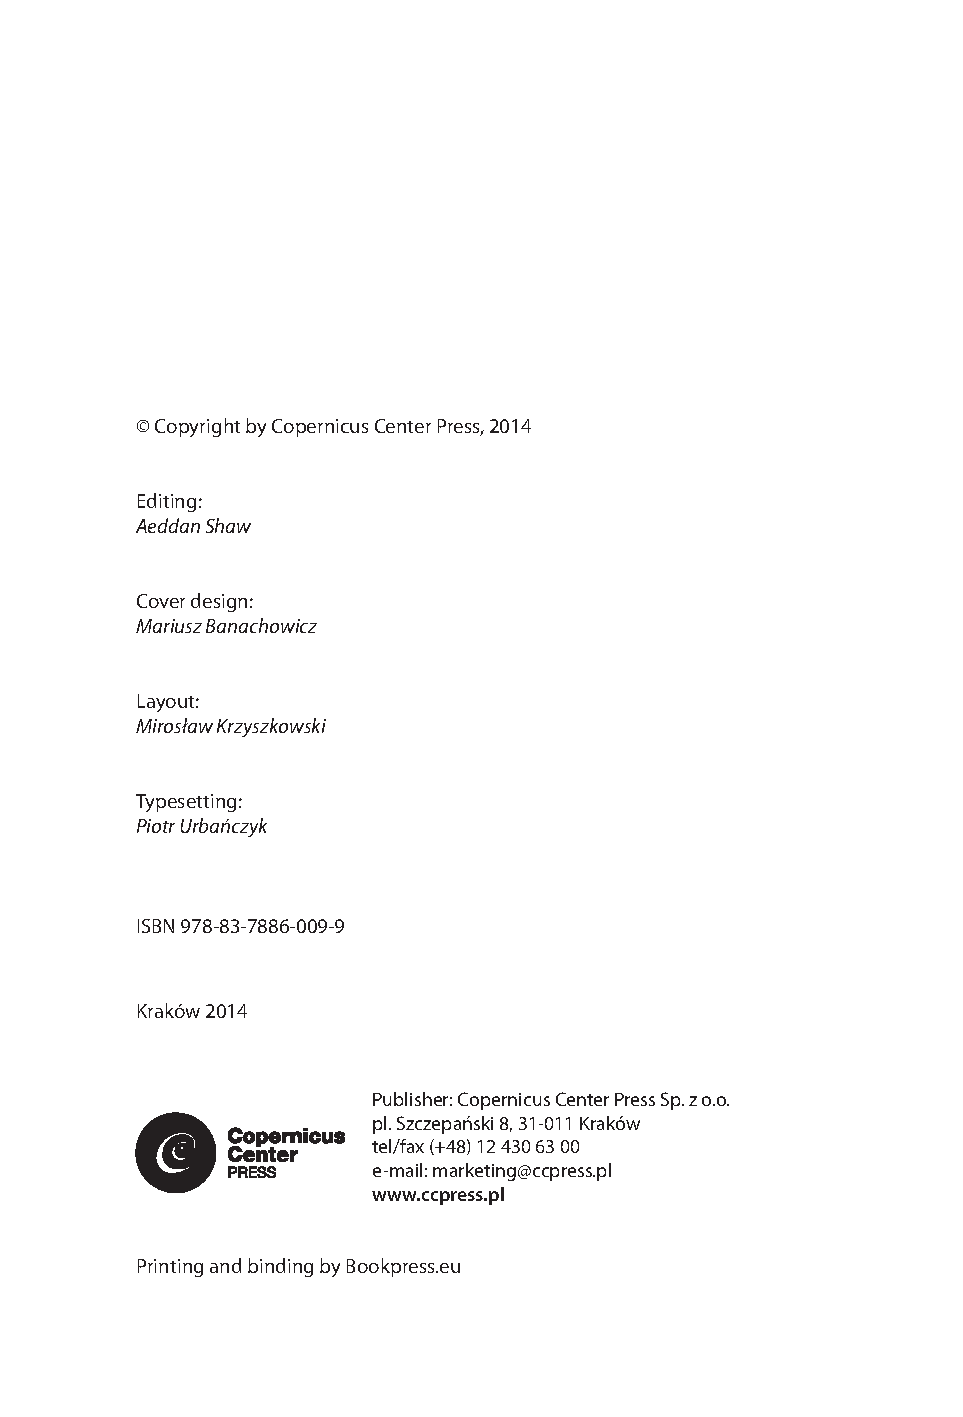
\includepdf[pages=1]{images/CT4.pdf}


\thispagestyle{empty}
\vspace*{1.2in}%
\begin{flushright}
\rectitle{Zagadnienia Filozoficzne\\w Nauce}\par
\vspace*{.5in}%
\chaptitleeng{Philosophical Problems\\in Science}\par
\end{flushright}
\vfill
\clearpage

\thispagestyle{empty}

\vfill

\noindent\begin{czw}© Copernicus Center Press, \rok\end{czw}

\vfill

\begin{adres}
	\begin{pagname}\noindent\begin{czwad}Editorial Board\end{czwad}\\
		Editor-in-Chief: dr hab. Paweł Jan Polak\\
		Deputy Editor-in-Chief: dr hab. Janusz Mączka\\
		Honorary Editor: prof. dr hab. Michał Heller\\
		Editorial Secretary: Piotr Urbańczyk\\
		Section Editor (\textit{Emergence of the Classical}): dr Michał Eckstein
	\end{pagname}
\end{adres}


\vfill

\noindent\begin{czw}Cover design: Mariusz Banachowicz\end{czw}

\vskip.5em

\noindent\begin{czw}Adjustment and correction: Artur Figarski\end{czw}

\vskip.5em

\noindent\begin{czw}Technical editor: Artur Figarski\end{czw}

\vskip.5em

\noindent\begin{czw}Typographic design: Piotr Urbańczyk\end{czw}

\vskip.5em

\noindent\begin{czw}Typeset in \end{czw}\LaTeX

%\noindent\begin{czw}Skład: Artur Figarski\end{czw}


\vfill

\begin{adres}
	\begin{pagname}\noindent ISSN 0867-8286 (print format)\\
		e-ISSN 2451-0602 (electronic format)
	\end{pagname}
\end{adres}

\vfill

\begin{adres}
		\noindent\begin{czwad}Editorial Office\end{czwad}
	
		\noindent\begin{pagname}Zagadnienia Filozoficzne w Nauce
		
		\noindent Wydział Filozoficzny UPJPII
		
		\noindent ul. Kanonicza 9, 31-002 Kraków
		
		\noindent POLAND
		
		\vskip.3em
		
		\noindent e-mail: zagadnienia@upjp2.edu.pl
		
		\noindent www.zfn.edu.pl\end{pagname}
\end{adres}

\vfill

\begin{wrapfigure}{L}{.3\textwidth}
	\noindent\includegraphics[width=.29\textwidth]{images/ccp.pdf}
%\noindent\includegraphics[width=.27\textwidth]{images/ccp.pdf}
\end{wrapfigure}
\vskip.4em
%\noindent\parbox[t]{6cm}{
\begin{adres}
	\noindent\begin{pagname}Publisher: Copernicus Center Press Sp. z o.o.
		
		\noindent pl. Szczepański 8, 31-011 Kraków POLAND
		
		\noindent tel. (+48) 12 448 14 12
		
		\noindent e-mail: marketing@ccpress.pl
		
		\noindent www.ccpress.pl\\ \end{pagname}
	
	
\end{adres}
%}




\clearpage

%	\thispagestyle{empty}
	\begin{flushright}%
	{\bigtitle{Zagadinienia\\Filozoficzne\\w Nauce\par}}%
	\vspace{0.2in}%
	{\chaptitleeng{Philosophical Problems in Science\par}}%
	\vspace{0.2in}%
	\hrule%
	{\LARGE\textbf{{\numerrzymski -- \rok}}}%
	\hrule%
	\end{flushright}%
%		\@mkboth{\czwit\contentsname}{\czwit\contentsname}%
	\vspace{0.5in}%
%
%\clearpage

%Spis tresci -------------------------------------------------

{\thispagestyle{plain} \tableofcontents \clearpage}
%--------------------------------------------------------------------------------------------
\newpage
\thispagestyle{plain}
\cleardoublepage
\thispagestyle{plain}

%--------------------------------------






%\ramkaart{Imię Nazwisko}
{Tytuł rozdziału.\\\chapsubtit{Podtytuł rozdziału}}
{Tytuł rozdziału. Podtytuł rozdziału}
{Tytuł rozdziału. Podtytuł rozdziału}

\lettrine[loversize=0.13,lines=2,lraise=0.00,nindent=0em,findent=0.2pt]%
{W}{}ielu filozofów i językoznawców twierdziło, że gdy identyfikujemy przedmioty, zarówno w języku, jak i w postrzeganiu, kierujemy się względami praktycznymi, potrzebami, wolą -- krótko mówiąc, swego rodzaju interesem, czy to gatunkowym (a więc ogólnoludzkim), czy to swoistym dla danej społeczności, cywilizacji czy jednostki. Wydaje się to kłócić z przeświadczeniem, że te przedmioty muszą istnieć, chyba że traktujemy to przeświadczenie jako jedną z wielu równouprawnionych wizji świata. Ta sama zasada wielości równosilnych perspektyw stosuje się a fortiori do języka metafizyki.

Tak więc powracamy tam, gdzie nasz horror bierze swój początek. Jakże mam trwać przy danym języku (czy jakimś szczególnym punkcie widzenia, z którego patrzę na świat, albo regule interpretacji całości doświadczenia), nie przyznając mu uprzywilejowanej poznawczej mocy? A jeśli pretenduję do dysponowania wyższym czy może nawet absolutnym językiem, to albo nadawałby się on tylko do mówienia o innych językach, nie zaś o rzeczywistości, do której się odnoszą, albo byłby standardowym językiem, a inne byłyby jego niekompletnymi dialektami. W tym drugim przypadku byłby to rzeczywiście boski język, absolutny i zawierający wszelkie wyobrażalne punkty widzenia. Lecz język taki jest niemożliwy; nawet Bóg, przemawiając ustami proroka, musiał się przełożyć na język ludzki; przekład jest niechybnie zniekształcony, a nam brak dostępu do oryginału. W przypadku pierwszym język mój (język pierwszego stopnia, język rzeczy) nie może wprawdzie rościć sobie pretensji do jakiejkolwiek pozycji uprzywilejowanej, lecz w tym języku nie sposób byłoby nieobecność owej pozycji wyrazić: by to uczynić, musiałbym swój język porzucić i przejść do super(czy meta-) języka -- ale w takim języku moje stanowisko, jako że szczególne, nie dałoby się wyrazić.

\myquote{
Gdy więc wielkodusznie powiadam: „wszystkie stanowiska metafizyczne są równie dobre”, sam żadnego stanowiska nie zajmuję, po prostu wyrażam zasadę tolerancji, która, jakkolwiek chwalebna, ma charakter formalny i nigdy nie wyda, czy choćby zainspiruje, żadnej metafizycznej idei. Lecz próbując zachować tę zasadę i obstawać zarazem przy swym szczególnym punkcie widzenia, popadam w niekonsekwencję, jako że twierdzę wtedy, iż „stanowisko moje jest tak samo dobre jak każde inne, mimo że jest nie do pogodzenia z żadnym innym”.

A jeśli tak mówię, nie mogę w zrozumiały sposób wyjaśnić, w jakim sensie to stanowisko jest moje, w przeciwieństwie do innych. Niestety, tolerancyjna wspaniałomyślność nie pozwala uciec od paradoksu samoodniesienia.
}

\noindent Leon Chwistek, logik i malarz, w wydanej w 1921 roku książce Wielość rzeczywistości sugerował istnienie czterech rodzajów wzajemnie niezależnych (a zatem przypuszczalnie nieinterferujących z sobą wzajem) rzeczywistości: rzeczy, takie jak je postrzega zdrowy rozsądek; rzeczy nauk fizycznych; wrażeń; i wyobraźni. Znajdują one swój artystyczny wyraz w malarstwie – odpowiednio: prymitywistycznym, naturalistycznym, impresjonistycznym, futurystycznym\footnote{To jest przypis dolny. Jeśli niezależne od siebie pokłady rzeczywistości wymagają dla swego opisu niezależnych języków, sugeruje to, że języki te są całkowicie nieprzekładalne; skoro tak, to w istocie można sądzić, że różne wizje świata współistnieć mogą w doskonałej wzajemnej obojętności}. Lecz wielość ta, dowodził, pozwala na dowolną liczbę równoprawnych poglądów na świat, z których żadnego nie można dowieść, lecz każdy jest do przyjęcia pod warunkiem, że nie próbuje zmonopolizować prawdy. Dopuszczalne stają się różne odpowiedzi na tradycyjne pytania, jak te o wolność woli, relację między ciałem a duchem, obiektywność wartości, jeśli zakres odniesienia ogranicza się do jednej lub niektórych spośród owych czterech rzeczywistości.

\noindent Leon Chwistek, logik i malarz, w wydanej w 1921 roku książce Wielość rzeczywistości sugerował istnienie czterech rodzajów wzajemnie niezależnych (a zatem przypuszczalnie
nieinterferujących z sobą wzajem) rzeczywistości: rzeczy, takie jak je postrzega zdrowy rozsądek

\section{Podtytuł 1 stopnia}

\noindent Teoria wielu -- jakkolwiek wyodrębnianych -- rzeczywistości, jeśli nawet w tym przypadku stworzona dla metafizycznej interpretacji malarstwa, proponuje przekonujący i kuszący obraz świata. Jednakże jako propozycja epistemologiczna nie jest w stanie -- czy to w wersji Chwistka, czy Williama Jamesa -- poradzić sobie z wciąż tą samą trudnością: jak dowieść wyższości pewnej teorii bytu w tym samym języku, w którym została wypowiedziana? Mieliżbyśmy utrzymywać, że twierdzenie „wszystko jest konieczne” jest równie prawomocne co twierdzenie „poza związkami logicznymi nic nie jest konieczne” i że doktryna, według której słowo „ja” nie ma odniesienia, jest nie mniej prawdziwa niż ta, wedle której cokolwiek ma odniesienie, jest względne w stosunku do „ja”?

\subsection{Podtytuł 2 stopnia}

\noindent Jeśli niezależne od siebie pokłady rzeczywistości wymagają dla swego opisu niezależnych języków, sugeruje to, że języki te są całkowicie nieprzekładalne; skoro tak, to w istocie można sądzić, że różne wizje świata współistnieć mogą w doskonałej wzajemnej obojętności: nie mogą być ze sobą konfrontowane ani między sobą sprzeczne. Ale twierdzenie, że nie mogą być konfrontowane, jest wyrażone w języku innym, wyższego stopnia, nie nadającym się do celów metafizycznych. I tu powraca ten sam kłopot: albo ograniczamy się do tego wyższego języka i wtedy werdykty nasze nie mają znaczenia dla rzeczywistych problemów, z których filozofia żyje, albo przyjmujemy pewną metafizyczną perspektywę i głosimy, że perspektywy tej, jako zamkniętej, nie da się zharmonizować z żadną inną ani też innej przeciwstawić -- i wtedy też, w wyniku tej samointerpretacji, perspektywa nasza jest bez znaczenia dla rzeczywistych problemów, z których filozofia żyje.

\sectionno{Podtytuł 1 stopnia}

\noindent Teoria wielu -- jakkolwiek wyodrębnianych -- rzeczywistości, jeśli nawet w tym przypadku stworzona dla metafizycznej interpretacji malarstwa, proponuje przekonujący i kuszący obraz świata. Jednakże jako propozycja epistemologiczna nie jest w stanie -- czy to w wersji Chwistka, czy Williama Jamesa -- poradzić sobie z wciąż tą samą trudnością: jak dowieść wyższości pewnej teorii bytu w tym samym języku, w którym została wypowiedziana? Mieliżbyśmy utrzymywać, że twierdzenie „wszystko jest konieczne” jest równie prawomocne co twierdzenie „poza związkami logicznymi nic nie jest konieczne” i że doktryna, według której słowo „ja” nie ma odniesienia, jest nie mniej prawdziwa niż ta, wedle której cokolwiek ma odniesienie, jest względne w stosunku do „ja”?

\subsection{Podtytuł 2 stopnia}

\noindent Jeśli niezależne od siebie pokłady rzeczywistości wymagają dla swego opisu niezależnych języków, sugeruje to, że języki te są całkowicie nieprzekładalne; skoro tak, to w istocie można sądzić, że różne wizje świata współistnieć mogą w doskonałej wzajemnej obojętności: nie mogą być ze sobą konfrontowane ani między sobą sprzeczne. Ale twierdzenie, że nie mogą być konfrontowane, jest wyrażone w języku innym, wyższego stopnia, nie nadającym się do celów metafizycznych. I tu powraca ten sam kłopot: albo ograniczamy się do tego wyższego języka i wtedy werdykty nasze nie mają znaczenia dla rzeczywistych problemów, z których filozofia żyje, albo przyjmujemy pewną metafizyczną perspektywę i głosimy, że perspektywy tej, jako zamkniętej, nie da się zharmonizować z żadną inną ani też innej przeciwstawić -- i wtedy też, w wyniku tej samointerpretacji, perspektywa nasza jest bez znaczenia dla rzeczywistych problemów, z których filozofia żyje.

\section{Podtytuł 1 stopnia}

\noindent Teoria wielu -- jakkolwiek wyodrębnianych -- rzeczywistości, jeśli nawet w tym przypadku stworzona dla metafizycznej interpretacji malarstwa, proponuje przekonujący i kuszący obraz świata. Jednakże jako propozycja epistemologiczna nie jest w stanie -- czy to w wersji Chwistka, czy Williama Jamesa -- poradzić sobie z wciąż tą samą trudnością: jak dowieść wyższości pewnej teorii bytu w tym samym języku, w którym została wypowiedziana? Mieliżbyśmy utrzymywać, że twierdzenie „wszystko jest konieczne” jest równie prawomocne co twierdzenie „poza związkami logicznymi nic nie jest konieczne” i że doktryna, według której słowo „ja” nie ma odniesienia, jest nie mniej prawdziwa niż ta, wedle której cokolwiek ma odniesienie, jest względne w stosunku do „ja”?

\subsection{Podtytuł 2 stopnia}

\noindent Jeśli niezależne od siebie pokłady rzeczywistości wymagają dla swego opisu niezależnych języków, sugeruje to, że języki te są całkowicie nieprzekładalne; skoro tak, to w istocie można sądzić, że różne wizje świata współistnieć mogą w doskonałej wzajemnej obojętności: nie mogą być ze sobą konfrontowane ani między sobą sprzeczne. Ale twierdzenie, że nie mogą być konfrontowane, jest wyrażone w języku innym, wyższego stopnia, nie nadającym się do celów metafizycznych. I tu powraca ten sam kłopot: albo ograniczamy się do tego wyższego języka i wtedy werdykty nasze nie mają znaczenia dla rzeczywistych problemów, z których filozofia żyje, albo przyjmujemy pewną metafizyczną perspektywę i głosimy, że perspektywy tej, jako zamkniętej, nie da się zharmonizować z żadną inną ani też innej przeciwstawić -- i wtedy też, w wyniku tej samointerpretacji, perspektywa nasza jest bez znaczenia dla rzeczywistych problemów, z których filozofia żyje.

\begin{thebibliography}{00}{Imię Nazwisko}
{Tytuł rozdziału. Podtytuł rozdziału}

\makeatletter
    \clubpenalty10000
    \@clubpenalty \clubpenalty
    \widowpenalty10000
\makeatother


\bibitem{Abc}
A.~Abc, \textit{Abc}...

\bibitem{Xyz}
A.~Abc, \textit{Abc}...

\end{thebibliography}





\sekcja{Od Redakcji}{Editorial}

\begin{editorial}{Michał Heller}
	{40 lat~-- sprężystość młodości i~doświadczenie wieku}
	{40 lat~-- sprężystość młodości i~doświadczenie wieku}
	{40 lat~-- sprężystość młodości i~doświadczenie wieku}
%	{Copernicus Center for Interdisciplinary Studies}
	{40 years of ZFN – the flexibility of youth and the experience of age}
%	{Abstrakt lorem ipsum}
%	{słowo, słowo.}




\lettrine[loversize=0.13,lines=2,lraise=-0.03,nindent=0em,findent=0.2pt]%
{R}{}óżne rocznice skłaniają do historycznych refleksji. Wprawdzie czterdzieści lat od jakiegoś wydarzenia nie zwykło
się specjalnie świętować, ale w~przypadku naukowego czasopisma jest to już na tyle długi okres, że warto mu poświęcić
chwilę zamyślenia.

\textit{Zagadnienia Filozoficzne w~Nauce} zaczynały skromnie, ale ambitnie: od zgrzebnego formatu typu ,,samizdat''
(bibułowy papier, powielacz), poprzez pierwsze przymiarki do komputerowego druku (nadal bibuła), aż do postaci naprawdę
drukowanej. Kolejne numery \textit{Zagadnień} są wiernym świadkiem stopniowych postępów w~polskiej, pokomunistycznej
sztuce drukarskiej: najpierw druk oszczędny, na miarę dostępnych technik, potem stopniowe ulepszenia, by wreszcie dojść
do wysmakowanego, nawet trochę snobistycznego, układu graficznego.

Tytuł \textit{Zagadnienia Filozoficzne w~Nauce} od samego początku zapowiadał pewien filozoficzny program. Że ma to
być coś o~wzajemnych relacjach nauki i~filozofii~-- było oczywiste, ale akcent nie był położony ani na ,,zagadnieniach
filozoficznych'', ani na ,,nauce'', lecz na przyimku ,,w''. Filozofia nauki jest~-- i~była już wtedy~-- dobrze rozwiniętą
dyscypliną filozoficzną. Miała swoje liczne szkoły i~odmiany. Najbardziej wpływową do dziś pozostaje filozofia nauki
zwana (nie całkiem merytorycznie poprawnie) anglosaską lub analityczną, ale analizy metodologiczne wywodzące się z~Filozoficznej
Szkoły Lwowsko-Warszawskiej także cieszyły się~-- i~nadal cieszą się~-- niemałym poważaniem. Założycielom
czasopisma chodziło o~coś innego, o~to jak tradycyjne pytania filozoficzne są obecne w~badaniach naukowych i~ich
rezultatach. Tradycyjna filozofia, stworzona przez Greków i~przetworzona przez europejską myśl średniowieczną nie tylko
wydała z~siebie nowożytne nauki empiryczne, lecz również wycisnęła na nich swoje ślady. Odczytywanie tych śladów i~odcyfrowywanie
ich znaczeń jest pasjonującym zadaniem, którego zaniedbanie byłoby niepowetowaną stratą dla współczesnej
kultury. Z~czasem dla tego typu uprawiania filozofii przyjęła się nazwa ,,filozofia w~nauce''~-- nie ,,filozofia nauki'',
lecz właśnie ten mały przyimek ,,w''.

Jest rzeczą oczywistą, że do realizowania w~ten sposób zarysowanego programu niezbędne jest wykorzystywanie środków
poznawczych i~metodologicznych narzędzi wypracowanych przez filozofię nauki. To jednak nie wszystko. Ślady
filozoficznych pytań rzadko leżą na powierzchni wytworów nauki. Nie jest więc tak, że aby je odczytać, wystarczy
przywołać znajomość tradycyjnej filozofii i~zastosować odpowiednie metodologiczne narzędzia. Filozoficzne tropy
prowadzą często w~głąb naukowych teorii, ich inspiracji i~wniosków. Do tego niezbędna jest dogłębna znajomość samej
nauki (najlepiej, jeżeli wynika ona z~twórczego jej uprawiania). Tylko wnikając głęboko w~tkankę naukowych teorii,
można zidentyfikować ich filozoficzne uwarunkowania i~poddać je trafnej interpretacji

Potrzebne jest także jeszcze inne wsparcie. Historia nauki nie tylko wiąże naukę, poprzez jej rodowód, z~tradycją
filozoficzną, lecz także bardzo skutecznie naprowadza na filozoficzne pozostałości w~dzisiejszych naukowych
dokonaniach. Dlatego też ,,filozofia w~nauce'' ściśle wiąże się z~historią nauki. W~tym mariażu historia nauki nie
sprowadza się do odtwarzania dziejów naukowych odkryć, lecz staje się aktywnym narzędziem badania.

Nawet pobieżne przejrzenie spisów treści poszczególnych numerów \textit{Zagadnień Filozoficznych w~Nauce}
przekonuje, że wśród autorów tego pisma pojawiają się: filozofowie, filozofowie nauki, historycy nauki, matematycy,
fizycy, astronomowie, biologowie i~przedstawiciele innych nauk. Dobre czasopismo to nie tylko kolejne numery drukowane
na papierze lub pojawiające się w~Internecie, lecz także środowisko, jakie wokół niego się skupia~-- kształtuje je i~samo
jest przez nie kształtowane. W~Krakowie, przynajmniej od końca dziewiętnastego wieku, żywe są tradycje
,,filozofujących uczonych'' i~dialogu między przedstawicielami różnych nauk a~filozofami. Kluczowymi pod tym względem są
takie postacie jak: Tadeusz Garbowski, Władysław Heinrich, Joachim Metallmann, Marian Smoluchowski, Władysław
Natanson\mydots\ \textit{Zagadnienia} wpisują się w~zapoczątkowaną przez nich tradycję i~pozwalają jej promieniować poza
Kraków.

Czasopisma tym różnią się od książek, że przeczytaną książkę po prostu odkłada się na półkę, a~czasopismo odradza
się z~każdym nowym numerem i, jeżeli jest dobrze wrośnięte w~środowisko, mimo iż przybywa mu lat, zachowuje sprężystość
młodości i~wzbogaca ją doświadczeniem dojrzałego wieku.
%\begin{flushright}
%	Kraków, 22 lutego 2019 roku
%\end{flushright}

{\raggedleft Kraków, 22 lutego 2019 roku\par}%



%Michał Heller

\end{editorial}



\sekcja{Emergence of the Classical}{Emergence of the Classical}

\begin{artengenv2auth}{Jerzy Kr\'ol, Torsten Asselmeyer-Maluga}
	{Topology and models of ZFC at early Universe}
	{Topology and models of ZFC at early Universe}
	{Topology and models of ZFC at early Universe}
	{\textsuperscript{1}University of Information Technology and Management, Rzesz\'ow, Poland\\
		\textsuperscript{2}German Aerospace Center (DLR), Berlin, Germany}
	{Recently the cosmological evolution of the universe has been considered where 3-dimensional spatial topology undergone drastic changes. The process can explain, among others, the observed smallness of the neutrino masses and the speed of inflation. However, the entire evolution is perfectly smooth from 4-dimensional point of view. Thus the raison d'{\^e}tre for such topology changes is the existence of certain non-standard 4-smoothness on $\mathbb{R}^4$ already at very early stages of the universe. 
		We show that the existence of such smoothness can be understood as a byproduct of the quantumness of the origins of the universe. Our analysis is based on certain formal aspects of the quantum mechanical lattice of projections of infinite dimensional Hilbert spaces where formalization reaches the level of models of axiomatic set theory. }
	{Cosmological model, Exotic $R^4$ and $S^3 \times \mathbb{R}$ in cosmology, 4-exotic smoothness, Models of ZFC, Topological model for inflation, Topological model for neutrino masses, Forcing, QM lattice of projections.}
	{%
		{\flushright\subbold{Jerzy Kr\'ol}\\\subsubsectit\small{University of Information Technology and Management, Rzesz\'ow, Poland}\par}%
		{\flushright\subbold{Torsten Asselmeyer-Maluga}\\\subsubsectit\small{German Aerospace Center (DLR), Berlin, Germany}\par}%
	}









\section{Introduction}
\lettrine[loversize=0.13,lines=2,lraise=-0.05,nindent=0em,findent=0.2pt]%
{T}{}here exist many free parameters of physics which can be determined experimentally though fundamental theoretic derivation of them is still missing. Moreover, knowing such derivation presumably will lead to the fundamental revolution in physics which would rely both on the extension of the standard model of particles (e.g. \cite{Weinberg2018}) and understanding gravity at quantum regime through cosmological data (e.g. \cite{Woodard2014}). Among the parameters in question there are masses of elementary particles, mixing angles, coupling constants and in cosmology the value of the cosmological constant, the speed of inflation or the $\alpha$ parameter in the Starobinsky model. For example we have experimental bounds on the neutrinos masses from PLANCK, Baryon Acoustic Oscillations (BAO) and KamLAND-Zen (Majorana neutrino) experiments \parencite{Neutrino-mass-KmLAND-Zen2016,PlanckCosmoParam2015,Neutrino2015}. The smallest experimental bound for the sum of the three neutrino masses reads
\[ \sum_i m_{\nu_i}\leq 0,12eV\,.\]
A way how these bounds were obtained indicate strongly that successful predicting true values for the masses should deal with cosmology. That is why the following question is in order.

\myquote{
Q1: Do we know any candidate for the model of cosmological evolution which would help determining theoretically the realistic (bound for) neutrino masses?    
}

We do know the seesaw mechanism of generating small neutrino masses, however, the derivation deals with two energy scales as free parameters which are not, however, fundamentally fixed. The Q1 has been answered in the affirmative in the series of papers \parencite{AK2018,AK2014,AK2019} where a suitable cosmological model has been constructed. Hence the immediate additional problem emerges:

\myquote{
Q2: Does the model of Q1 predicts realistic values of some inflationary parameters, like a speed of inflation?
}

The affirmative answer for Q2 has been indeed given recently. The model is based on a smooth differential structure on $\mathbb{R}^4$ which is not standard, i.e. is not any smooth product $\mathbb{R}\times\mathbb{R}^3$. We call such a structure an exotic smooth structure and $\mathbb{R}^4$ with it an exotic $R^4$. There exist infinitely continuum many such different, pairwise nondiffeomorphic, exotic $R^4$'s. Thus mathematics favours dimension 4 in this respect, i.e. any other $\mathbb{R}^n$ for any $n\neq 4$ carries {\em unique} standard smooth structure. The physics of the proposed cosmological model distinguishes one of the structures, namely the one which embeds in, also exotic, K3 surface, i.e.
\[R^4\hookrightarrow K3\oplus \overline{{\rm CP}}^2\,.  \]

\myquote{
Q3: K3 is compact. Does it have any physical, probably cosmological, meaning which would extend the embedded noncompact $R^4$ representing spacetime?
}
After presenting some details of the model we will present certain speculative ideas regarding this issue.

In the second part of the paper we will deal with quantum origins of the smoothness required by the model. Provided, the initial state of the Universe is quantum mechanical, i.e. formulated as usual by a Hilbert space of states, we will analyze the following problem:

\myquote{
Q4: Does the QM formalism know that the universe at large scales is smooth, 4-dimensional and exotic? 
}

Similar question has been recently addressed in \parencite{JKuniverse17,JK2017a}. More thorough analysis will be given elsewhere. We show that the smoothness on $\mathbb{R}^4$, which agrees with QM formalism, has to be exotic. This result strongly supports the proposed model. Questions Q1 and Q2 along with the details of the model will be presented in the next section. The results and arguments concerning Q4 will appear in the subsequent section. We close the paper with the discussion which covers also Q3.

\section{The smooth cosmological model for inflation and neutrino masses}\label{sec:2}
%It is quite successful scenario to apply the Friedman-Robertson-Walker (FRW) cosmology for describing large scale universe with its homogeneous and isotropic structure.
The Friedman-Robertson-Walker (FRW) model has proven to be very successful in modelling a homogeneous and isotropic universe.
The time-like slices define 3-geometries which, in the case of the closed universe, are 3-spheres $S^3$ ($k=+1$) giving rise to the model based on $S^3\times \mathbb{R}$. Since 1979 seminal work by M. H. Freedman \parencite*{Freedman1979} mathematicians have become aware of the existence and basic constructions of smooth manifolds which all are topologically $S^3\times \mathbb{R}$, however, smoothly they are not diffeomorphic neither to each other nor to $S^3\times \mathbb{R}$. Soon after in 1980s mathematicians again found that similar open 4-manifolds exist also for $\mathbb{R}^4$---exotic $R^4$'s. They all are homeomorphic to $\mathbb{R}^4$ being pairwise nondiffeomorphic. Moreover, there is a continuum of mutually nondiffeomorphic classes of exotic open \mbox{4-manifolds} each being homeomorphic with a given open 4-manifold (see e.g. \cite{GS1999}). This and the existence of exotic $R^4$ make the dimension 4 completely distinguished in mathematics unlike the other dimensions where the usual tools of differential geometry and topology work well. Many new techniques have been found and developed within the recent years to understand and explore the phenomenon of exotic 4-smoothness. Among which Casson handles, Akbuluth corks, tools of hyperbolic geometry, handle calculus and many others have become an everyday toolkit of researchers in the field. We do not know any way how to avoid these constructions and replace them by known techniques from other dimensions. That is why it is not a surprise that the variety of methods are being applied in order to recognize physical applications of 4-exotic smooth structures. Two aspects are particularly promising---the dimension 4 is also distinguished by physics and several parameters in cosmology and particle physics call for their fundamental derivation and explanation. 

On the way of searching for such an explanation we have recently proposed the cosmological model based on exotic $S^3\times \mathbb{R}$, i.e. $S^3\times_{\Theta}\mathbb{R}$ \parencite{AK2018,AK2014,AK2019}. Such smooth open 4-manifolds (infinite continuum many of them) can be seen as submanifolds (exotic ends) of exotic $R^4$'s
\[ S^3\times_{\Theta} \mathbb{R}\subset R^4\,. \]
Here $\Theta$ refers to certain homology 3-sphere smoothly embedded in exotic $S^3\times_{\Theta} \mathbb{R}$
and allows for distinguishing between these exotic smooth manifolds. When $\Theta = S^3$ the product is globally smooth and the 4-manifold becomes the unique standard smooth $S^3\times \mathbb{R}$. 
So the base for the cosmological model is to refer to these exotic smooth $S^3\times_{\Theta}\mathbb{R}$ rather than to the standard smooth $S^3\times \mathbb{R}$.
\begin{quotation}
Exotic $S^3\times_{\Theta}\mathbb{R}$ is a smooth 4-manifold, so the cosmic evolution seen from dimension 4 can be considered perfectly smooth. However, the 3-dimensional slices undergoes drastic topology changes
\begin{equation}\label{S3}S^3\overset{1.}{\to} \Sigma(2,5,7) \overset{2.}{\to}P\# P\,,  \end{equation}
which will determine the values of certain physical parameters like neutrino masses.

The 3-dimensional evolution within the standard $S^3\times \mathbb{R}$ is trivially $S^3\to S^3\to S^3$.
\end{quotation}
Here $\Sigma(2,5,7)$ is the Brieskorn homology 3-sphere and $P\# P$ is the connected sum of two copies of the Poincar{\'e} 3-sphere \parencite{AK2018,AK2019}. To pinpoint physics into the model we are taking the radius of $S^3$ in (\ref{S3}) to be of order of the Planck length and the natural energy of that epoch to be Planck energy. Such a choice is natural since the evolution of the universe should start with the quantum Planck era. The topology change 1. is the 4-dimensional cobordism $W(S^3,\Sigma(2,5,7))$ between 3-sphere and the Brieskorn sphere. To make it smooth we need to glue a Casson handle. A Casson handle (Ch) is the infinite geometric construction which becomes the main player in investigating of 4-exotic smoothness. As shown by Freedman every Ch is topologically the ordinary 2-handle, $D^2\times \mathbb{R}^2$, with the attaching region $S^1\times \mathbb{R}^2$ while smoothly there are infinitely many of different exotic Ch's (e.g. \cite{GS1999}). The infinite geometric construction present within any Ch is naturally grouped into the layers indexed by $n\in \mathbb{N}$ and each layer corresponds to the level of a labeled tree defining Ch. Each level $n$ contributes topologically to the change of the length scale by the expression $\sim \frac{\theta^n}{n!}$. $\theta$ is the function of purely topological invariant of the 3-manifold $\Sigma(2,5,7)$, i.e. $\theta =\frac{3}{2\cdot CS(\Sigma(2,5,7))}$ where in the denominator stands Chern-Simons invariant of the Brieskorn homology sphere. The contribution of the entire infinite Casson handle is thus given by \parencite{AK2018,AK2014,AK2019}
\begin{equation}\label{exp1} a=a_0\sum_{n=0}^{\infty}\frac{\theta^n}{n!}\,. \end{equation}
To determine the energy scale of the first topology change 1. in (\ref{S3}) relies on finding the minimal segment of Ch which has to be develop in order to make the cobordism $W(S^3,\Sigma(2,5,7))$ smooth in $S^3\times_{\Theta}\mathbb{R}\subset R^4$. As argued in \parencite{AK2014,AK2019} on the base of Freedman result there are needed 3-stages of Ch: Every Ch is embeddable in its first 3-stages. Thus the shortest possible time change, coordinatized by the levels $n$, reads \parencite{AK2014,AK2019} 
\[ \Delta t= \big(1+ \theta + \frac{\theta^2}{2}+\frac{\theta^3}{6}\big)\cdot t_{\rm Planck} \]
which is the shortest change lowering the Planck energy. This gives rise to the first, below Planck, energy scale
\[E_{\rm GUT}= \frac{E_{\rm Planck}}{1+ \theta + \frac{\theta^2}{2}+\frac{\theta^3}{6}}\,. \] 
Calculating $\theta$ as a function of Chern-Simons invariant, $\theta=\frac{140}{3}$, gives rise to the GUT scale, i.e. $E_{\rm GUT}\simeq 0,67\cdot 10^{15}\, {\rm GeV}$. But this time it is a purely topologically determined energy scale (up to the initial Planck energy). 

Let us turn to the second topology transition in (\ref{S3}), i.e. $\Sigma(2,5,7)\to P\#P$. To make it smooth we need to glue in three Ch's. This is due to the topological decomposition of the boundary of $E8\oplus E8$ as K3 surface $E(2)$ \parencite{AK2018,AK2019}. Thus the second topology change follows from the embedding of exotic $R^4$ into $E(2)\# \overline{CP^2}$. Taking into account the entire infinite stages of these Ch's, and relating the result to the initial Planck energy, gives rise to the result 
\[E_2=\frac{E_{\rm Planck}\cdot \exp\big(-\frac{1}{2\cdot CS(P\# P)}\big)}{1+\theta +\frac{\theta^2}{2}+\frac{\theta^3}{6}}\,. \]
This energy $E_2\simeq 63\, {\rm GeV}$ is of the order of the electroweak energy scale (or the half of the Higgs mass). Again, the result is supported topologically and the exotic smoothness of $R^4$ is the main reason for this support. 

Given the two topological energy scales we are using them to evaluate the neutrino masses. Applying the simplest seesaw mechanism we are taking the mass matrix 
\[
\left(\begin{array}{cc}
0 & M\\
M & B
\end{array}\right)
\] with energy scales $M\sim {E\rm GUT}\simeq 0,67\cdot 10^{15}\, {\rm GeV}$ and $B\sim E_2\simeq 63\, {\rm GeV}$ introduced. Then the mechanism relies on calculating the eigenvalues which read \[
\lambda_{1}\approx B\qquad\lambda_{2}\approx-\frac{M^{2}}{B},
\] thus the neutrino mass is predicted as 
\[m=\lambda_2\simeq 0,006\, {\rm eV}.   \] The value agrees with the current experimental upper-bounds (e.g. \cite{PlanckCosmoParam2015,Neutrino2015}). It is, however, the value protected by the topology of the unverse which underlies certain nonstandard (exotic) smooth differentiable structure of $R^4$. 

It is quite interesting that the formula (\ref{exp1}) allows for determining the $e$-folds number $N$ for the inflation in such a topological model \parencite{AK2014,AK2019}. Namely
\[N=\frac{3}{2\cdot CS(\Sigma(2,5,7))} + \ln 8 \pi^2 \simeq 51 \] which is experimentally acceptable and, as the model explains, it is again topologically supported value.
\section{Very early universe and the evolution of the models of ZFC}
We have seen that
%exotic smoothness on $S^3\times \mathbb{R}$ replacing the standard one
the replacement of the standard smooth structure by the exotic one $S^3\times \mathbb{R}$
has tremendous impact on understanding of the cosmological evolution of the universe and leads to determining neutrino masses along with GUT and electroweak energy scales. All this relies upon the initial conditions settled as quantum Planck energy scale and the Planck length radius of $S^3$ so that the question Q4 from the Introduction can be addressed. Namely, does QM formalism determine the large scale smoothness of the evolving universe? Is this smoothness in dimension 4 indeed exotic or rather standard? If the answers indeed support an exotic geometry that would be a strong indication in favour of the entire model. The key tool to attack this problem is {\em formalization}: one goes back to a formal level where set theoretic constructions of QM and differential geometry become important. Especially instead of working in undetermined formally universal space one starts working in specific models of Zermelo-Fr\"ankel set theory with the axiom of choice (ZFC). The models can vary along the evolution of the universe and their relations serve as additional physical degrees of freedom. 

Let ${\cal H}$ be an infinite dimensional separable complex Hilbert space representing states of the quantum world at the Planck era. Infinite dimensionality is enforced by the need to refer to spacetime with momentum and position operators. Then let $\{\bf{L},\wedge,\vee,\neg, 0,1\}$ be the lattice of projections of ${\cal H}$. Local Boolean frames of the lattice are given by maximal complete Boolean algebras of projections $B$'s. If $\dim {\cal H}=\infty $ then each such $B$ is, in general, decomposed into the atomic, $B_a$, and atomless, $B_c$, parts \parencite{Kappos1969}
\begin{equation}\label{B} B=B_a \otimes B_c\,. \end{equation}
$B_c$ is the atomless measure Boolean algebra, i.e. $B_c\simeq {\rm Bor}([0,1])/{\cal N}$ where ${\rm Bor}([0,1])$ is the Borel algebra of subsets of $[0,1]\subset \mathbb{R}$ and ${\cal N}$ ideal of Lebesgue measure zero subsets of $[0,1]$. $B_c$ is homogenous, i.e. $B_c \overset{\rm iso}{\simeq} B_c(p)$ for every $p>0$ where $B_c(p)$ is the algebra of all $q\leq p$ with the unit $p$. It follows that $B_c$ is the universal algebra for all $B$'s which means that 
\[ \forall_{B\subset {\bf L}}\ B{\text{ is completely embeddable in }} B_c \,.\]
Thus in what follows we will use a single symbol $B$ for this atomless, complete, universal measure algebra, replacing the variety of $B$'s in (\ref{B}). 

Let $V$ be a transitive standard universe of set theory and $V^B$ the Boolean-valued class of ZFC (e.g. \cite{Jech2003}). Such a transitive standard model $V$ exists provided ZFC is consistent due to the Mostowski collapsing theorem \parencite{Jech2003}. The construction of $V^B$ is also well recognized and described in a variety of textbooks (see e.g. \cite{Jech2003,Bell2005}). For us $V^B$ is a Boolean-valued model which gathers together Boolean frames $B$'s derived from ${\bf L}$. Maximal complete Boolean algebras $B$'s determine maximal sets of commuting observables of QM based on ${\cal H}$ by virtue of the spectral theorem. Let $\{A_i,i\in I\}$ be a set of commuting observables on ${\cal H}$. The maximality of such a family is equivalent to the existence of a single self-adjoint operator $A$ with the spectral measure $\mu_{\sigma}$ on $S(A)$---the Stone spectrum of the projection algebra $B$. To every set $\{A_i,i\in I\}$ as above there exists a Boolean algebra of projections $B$ with the spectrum $S(A)$. The algebra $B$ generates all observables in the family in the sense that the projections being the values of the spectral measures live in $B$. In the case $B$ of being maximal the family of observables is also maximal (complete) set of observables. Let $L^2(S(A),\mu_{\sigma})$ be the Hilbert space of square $\mu_{\sigma}$-integrable complex-valued functions on $S(A)$. 
\begin{Lemma}\parencite{Boos1996}
The following statements are equivalent:
\begin{itemize}
    \item[i.] There exists a unitary isomorphism $U:{\cal H}\to L^2(S(A),\mu_{\sigma})$ such that 
    \[UAU^{-1}(\psi(x))=x\psi(x)
    \] is the self-adjoint position operator $Q$ on $L^2(S(A),\mu_{\sigma})$.
\item[ii.]  $A$ is maximal.
\item[iii.] $B$ is complete and maximal.
\item[iv.] Every self-adjoint operator $C$ on ${\cal H}$ commuting with $B$, fulfills $C=f(A)$ for some Borel function $f:S(A)\to \mathbb{R}$.
\end{itemize}
\end{Lemma}
We see that there is a strict $1:1$ correspondence between frames of complete sets of self-adjoint operators and maximal Boolean algebras $B$'s. Now let us assign the maximal operator $A$ to every self-adjoint $C$ on ${\cal H}$.
%Subsequently there corresponds to $A$ the maximal complete Boolean algebra $B$.
Subsequently, there is a maximal complete Boolean algebra $B$, which corresponds to $A$.
The important, though obvious, consequence is the following
\begin{Corollary}\label{corr1}
In QM one cannot reduce the resulting family of $B$'s as above to the single-element family $\{B\}$.
\end{Corollary}
The reason is that there exist noncommuting observables determining different maximal families which correspond to different maximal complete Boolean measure algebras $B$'s. Otherwise the correspondence would not be $1:1$.

Now let us assign the family of copies of $V^B$'s to $B$'s according to the lemma above. Again the assignment is irreducible to a single model $V^B$ even though the models $V^B$'s are isomorphic. Each $V^B$ is a Boolean-valued model of ZFC. To reduce it to a 2-valued model $V^{\{0,1\}}$ one should make use of certain homomorphisms \[h_B:B\to \{0,1\}\,. \] 
We want to preserve as much of the structure of $B$ as possible since these algebras are local frames of QM. Each $B$ is atomless complete maximal measure algebra. In particular given a subset $S\subset B$ there always exist maximum $\bigvee S\in B$. We say that $h_B$ preserves completeness of $B$ if for every family $S\subset B$ with $\bigvee S \in B$ ($B$ is complete)
\[h_B(\bigvee S)=\bigvee \{h_B(a):a\in S\}\,. \]
Moreover we want to preserve dense families in $B$. A subset $X\subset B$ is dense in $B$ when 
\begin{gather}
q\in X \wedge p\in B \wedge q\leq p \Rightarrow p\in X\\
\forall p\in B \exists q\in X (p\leq q)\,.    
\end{gather}
Particularly important families in $B$ are generic ultrafilters. A subset $X\subset B$ is a filter on $B$ when
\begin{gather}
  q_1, q_2\in X \Rightarrow \exists z\in X \; {\rm such\; that}\; q_1\leq z \wedge q_2 \leq z \\
 q\in X \wedge p\in B \wedge p\leq q \Rightarrow p\in X\,. 
\end{gather}

\begin{Definition}
A generic ultrafilter on $B$ is a filter ${\cal U}\subset B$ such that for any family $X\subset B$ dense in B
\[X\cap {\cal U}\neq \emptyset \,.  \]
\end{Definition}
Then, the following result hold.
\begin{Lemma}\parencite[p.35]{Solovay1970}\label{hB}
Let $h_B:B\to \{0,1\}$ be a complete homomorphism. Then 
\[h_B^{-1}(1)= {\cal U} \] is a generic ultrafilter on $B$.
\end{Lemma}
Let $V$ be the universe of sets as before and ${\cal U}\subset B$ a generic ultrafilter on $B$ i.e. ${\cal U}\cap X\neq \emptyset$ for every dense subfamily $X$ on $B$ in~$V$.
\begin{Lemma}\parencite[p.7]{Jech1986}\label{UB} $B$ is atomless iff ${\cal U} \notin V$.
\end{Lemma}
From Lemmas \ref{hB} and \ref{UB} it follows
\begin{Lemma}
In $V$: There does not exist any complete $h_B:B\to \{0,1\}$ for the measure algebra $B$.
\end{Lemma}
\begin{proof}$B$ is atomless so there does not exist any generic ${\cal U}$ in $B$ in~$V$.\end{proof}
One way to overpass this no-go property is to relativize ZFC into models of ZFC or allow for changing the universe of sets. Let $V$ be a standard transitive model of ZFC as above. We need two important conditions imposed on $B$ defined in $V$. If $B$ is a complete atomless Boolean algebra in $V$ and $P$ a dense partial order $P\subset B$ in $V$. Then, following \parencite{Solovay1970}, we assume that:
\begin{itemize}
    \item[1.] There exist only countably many subsets of $P$ in $V$.
    \item[2.] $h_B:B\to \{0,1\}$ is said to be $V$-complete if for every family $S\subseteq B$ living in $V$, i.e. $S\in V$, and $\bigvee S\in V$ then 
    \[ h_B(\bigvee S)=\bigvee\{h_B(s):s\in S \} .\]
    \item[3.] A filter ${\cal U}$ on $B$ is $V$-generic when ${\cal U}$ has nonempty intersection with every dense family in $V$.  
\end{itemize}
Then one proves
\begin{Lemma}\parencite[p.35]{Solovay1970}
For every $V$-complete homomorphism $h_B:B\to \{0,1\}$ the set 
\begin{equation}\label{hC} {\cal U}=\{x:h_B(x)=1\} \end{equation} is an $V$-generic filter on $B$.

Conversely, for any $V$-generic filter ${\cal U}$ there exists unique $h_B$ fulfilling (\ref{hC}).
\end{Lemma}
Note that for $B$ atomless still Lemma \ref{UB} forbids the existence of ${\cal U}$ in $V$ so that \[h_B\notin V \text{ and } {\cal U}\notin V\,. \] 
However, due to the relativization of models of ZFC in models of ZFC we can now indicate the model $V'$ extending the $V$ where there live both $h_B$ and ${\cal U}$. This is the random forcing extension of $V$.
\begin{Theorem}\parencite[p.36]{Solovay1970}\label{Th1}
There is a canonical 1:1 correspondence between the reals random over $V$ and $V$-complete homomorphisms of $B$, $h_B\to \{0,1\}$.
\end{Theorem}
As we noted before the Boolean-valued models $\{V^B: B\in {\cal B}\}$ are isomorphic. On the other hand these models cannot be reduced to a single-element family $V^B$. Given the procedure above reducing $B$ to $\{0,1\}$ we are faced with a family of trivially isomorphic algebras $\{0,1\}$ so that they are distinguished by different $V$-generic filters ${\cal U}$'s. As a result we have a family of pairs $\{(V^{\{0,1\}},{\cal U}_{\alpha})_{\alpha\in I}\} $. There exist, however, corresponding reductions of $V^B$ to 2-valued models as in the above family of pairs. This follows from Theorem \ref{Th1}.
\begin{Lemma}
The family $\{(V^{\{0,1\}},{\cal U}_{\alpha})_{\alpha\in I}\} $ is given by the random forcing extensions $\{ V[{\cal U}_{\alpha}], \alpha\in I$\}.  
\end{Lemma}
In this way we avoid just to duplicate isomorphic copies of $V^{\{0,1\}}$. Rather there are 2-valued forcing extensions $V[{\cal U}_{\alpha}]^{\{0,1\}}=V[{\cal U}_{\alpha}], \alpha\in I$ respecting 2-valued algebras and ultrafilters ${\cal U}_{\alpha}$.
Now we can give the construction of a spacetime manifold $M^4$ via local coordinate frames supported by the models of ZFC. Let $M^4$ be a smooth 4-manifold with a smooth atlas $\{ U_{\alpha}\simeq \mathbb{R}^4:\alpha \in J \}$.
\begin{Definition}\label{def1}
We call an atlas $\{ U_{\alpha}\simeq \mathbb{R}^4:\alpha \in J \}$ of $M^4$ {\bf L}-supported if for every $U_{\alpha}$ there exists $V$-generic ultrafilter ${\cal U}_{\alpha}$ and the model $V[{\cal U}_{\alpha}]$ such that the formalisations of $U_{\alpha}$ read
\begin{equation}\label{F} U_{\alpha}\simeq R^4_{V[{\cal U}_{\alpha}]}\,. \end{equation}
If for every local QM frame $B=B_{\alpha}\in {\cal B}$ and its corresponding 2-valued forcing reduction $V[{\cal U}_{\alpha}]$ every smooth atlas of $M^4$ contains all formalisations as in (\ref{F}), then we say that $M^4$ covers smoothly {\bf L}.  
\end{Definition}
Here $R_{V[{\cal U}_{\alpha}]}$ is the unique model of complete algebraically closed field of real numbers in the model $V[{\cal U}_{\alpha}]$.
\begin{Theorem}
If every atlas of a smooth $\mathbb{R}^4$ covers smoothly {\bf L} then such $\mathbb{R}^4$ cannot be the standard smooth $\mathbb{R}^4$.
\end{Theorem}
\begin{proof}
The family $\{B_{\alpha}\}$ of QM frames is not any single-element family (see Corollary \ref{corr1}) so thus the families of $\{V^{B_{\alpha}}\}$ and its 2-valued reductions $\{V[{\cal U}_{\alpha}]\}$. From the smooth covering of {\bf L} property as in Definition \ref{def1} every smooth atlas on $\mathbb{R}^4$ contains a family of $\{U_{\alpha}\}$ with the corresponding formalisations $\{U_{\alpha}\simeq R^4_{V[{\cal U}_{\alpha}]} \}$. Thus every smooth atlas cannot be a single-chart one. 
So we have smooth $\mathbb{R}^4$ whose none smooth atlas is single-chart. Now it is enough to note that any smooth $\mathbb{R}^4$ which is diffeomorphic to the standard $\mathbb{R}^4$ assumes 1-chart smooth atlas. Otherwise it would not be diffeomorphic to the standard $\mathbb{R}^4$.
\end{proof}
So to make agreement between smooth structure on $\mathbb{R}^4$ and QM lattice {\bf L} such that {\bf L} supports this structure requires referring to exotic $R^4$. The standard $\mathbb{R}^4$ cannot cover {\bf L}. If such an agreement took place in the real evolution of the universe the phenomenon of changing models of set theory from $V$ to the forcing extension $V[{\cal U}_{\alpha}]$ should also be a physical process. This more that as we saw in Sec. \ref{sec:2} certain exotic $R^4$ considered as input of the cosmological model allows for predicting the values of important physical parameters like GUT and electroweak energy scales and the neutrino masses. 

\section{Discussion}
One disturbing feature of the presented model is that the exotic $R^4$ generating reliable values of physical parameters is determined by the embedding 
\[R^4\subset K3\# \overline{CP^2}\,. \] What is a physical role ascribed to $K3\# \overline{CP^2}$? One possible answer is to see $R^4$ as a small part of the entire universe which remains outside of our observational capabilities. It is not excluded by current experiments (cf. \cite{AK2018}). However, accepting this point of view there remains the question about the origins of shape and compactness of the 4-dimensional large universe like $K3\# \overline{CP^2}$. One indication is the uniqueness of the $K3$ surface as Ricci flat Callabi-Yau manifold, without closed time-like loops. Possibly certain minimality conditions imposed from general relativity would enforce such structure of the universe. Moreover this is the peculiar and important prediction of our model that the universe at largest scales is compact and based on smooth (exotic) $K3$ surface.

Another possibility is the fundamental role ascribed to exotic \mbox{4-smoothness} on open 4-manifolds in the evolution of the universe, especially exotic $R^4$ and $S^3\times_{\Theta} \mathbb{R}$. This indicates rather technical and purely mathematical appearance of $K3\# \overline{CP^2}$ which, however, determines both spatial topological transitions supporting physical results. Anyway the model shows that exotic smoothness on open \mbox{4-manifolds} appears as new and fundamental tool for physics. Many unanswered so far questions of physics gain new formulations resulting in their resolutions.

It seems quite important to derive these exotic smooth manifolds directly from QM formalism. If succeeded the model would show very strong indication that the differential structure of 4-dimensional spacetime regions \emph{must} be exotic. We showed that the standard structure on large scales of the universe does not agree with QM. Similar approach, though using somewhat different techniques, have been proposed and developed already in \parencite{JKuniverse17,JK2017a}. 
The proposal here is an important step into this direction. There remains, however, to determine precisely this unique exotic $R^4\subset K3\# \overline{CP^2}$ from QM. 



\end{artengenv2auth}



\begin{artengenv}{Fedele Lizzi}
	{Points. Lack thereof}
	{Points. Lack thereof}
	{Points. Lack thereof}
	{\textls[-24]{Dipartimento di Fisica ``Ettore Pancini'', Universit\`{a} di Napoli Federico~II, Napoli, Italy;}\\
	INFN, Sezione di Napoli, Italy;\\
	Departament de F\'{\i}sica Qu\`antica i Astrof\'{\i}sica and Institut de C\'{\i}encies del Cosmos (ICCUB),
	Universitat de Barcelona, Barcelona, Spain}
	{I will discuss some aspects of the concept of ``point'' in quantum gravity, using mainly the tool of noncommutative geometry. I will argue that at Planck's distances the very concept of point may lose its meaning. I will then show how, using the spectral action and a high momenta expansion,  the connections between points, as probed by boson propagators, vanish. This discussion follows closely \parencite{Kuliva}.}
	{quantum geometry, localizability, Planck Scale.}
	



\lettrine[loversize=0.13,lines=2,lraise=-0.05,nindent=0em,findent=0.2pt]%
{I}{}n this contribution we will discuss, from the point of view of a physicist\footnote{I have provided an extensive literature, which is however by all means not complete. I often referred to our work, since it represents better the point of view presented here. For other relevant papers one may consult the references of the cited papers.}, a very classical concept: that of a \emph{point}. Although the concept is pervasive in physics and mathematics, as it often happens with the concept we think we know, its most profound meaning (beyond definitions) is far from easy. We encounter points very early in the study of mathematics. We remember that in our elementary school book a point was defined as: \emph{A geometrical entity without dimension}. We must confess that, after reading this definition, we were none the wiser about what a point is. The main reason could have been the belief what everyone kowns what  points are. They could produced at will with a biro. Or, better, with a sharper pin, or an even sharper object. In any case we could envisage a limiting process for which we could always find something more ``pointlike''.

Points are crucial in geometry, and Euclid himself gave a definition of them: \emph{"That which has no part"}. This is not always true, often we just find expedient to ignore possible internal structures and talk of points, indeed it may be that there are ``points'' which have a rich structure, which we ignore for the problem at hand. 
In astrophysics, for example, a point may be a galaxy, or even a cluster of galaxies. 
In general relativity the set of point is usually the set of possible localised \emph{events}. This certainly implies some structure. 
In classical ``point particle'' dynamics we use points of phase space to describe the state of motion of a particle, which we imagine pointlike. What we have in mind when we talk of points, or pointlike particles, is always the limiting process alluded before. There may be reasons, such as technological limitations or convenience, to consider pointlike something which is not, but at the end of the limiting process, operationally, at the bottom there are points.

It is well known that for particle phase space (the space of positions and momenta/velocities) this vision becomes untenable when one considers quantum mechanics. It is impossible to know at the same time position of momentum of a particle. This is the content of Heisenberg \emph{uncertainty principle} \parencite{Heisenberguncert}:
\be
\Delta p \Delta q \geq \frac\hbar2 . \label{Heisenberg}
\ee
For quantum phase space we have a well formed, successful theory, which is supported by a large body of experimental evidence, which we call \emph{Quantum Mechanics}. Although it may be formulated in several ways, by far the most useful, and rigorous, one is to consider all observables, and in particular position and momentum, to be part of the algebra of \emph{operators}. The notion of point, and with it that of trajectory, is not present anymore in the theory. Every manual of quantum mechanics at some stage attempts a connection with classical physics, see for example \parencite[Sect.~II.4]{Messiah}. But the notion of point of phase space is just  an ill defined quantity in quantum mechanics. The closest we may get to it is the possibility to have a \emph{coherent state}. Independently on the formal group theoretical definition (see for example \cite{Perelomov}), for our purposes it suffices the property that they are \emph{maximally localised} states, which will saturate the Heisenberg uncertainty bound~\eqref{Heisenberg} with the equality. A central role is played by the presence of a \emph{dimensional} quantity (Planck's constant $\hbar$) which acts as cutoff on phase space, thus avoiding the ``ultraviolet catastrophe".

Phase space has become a \emph{noncommutative geometry}, still it is possible to study the geometrical properties of such spaces, and this work has been pioneered by Alain Connes \parencite*{Connesbook}. The idea is to rewrite ordinary geometry in algebraic terms, for example substituting the category of topological spaces with that of $C^*$-algebras. A physicists would say that spaces are probed by the fields built on it. For commutative spaces points are pure states, i.e.\ normalised linear maps from the algebra to complex numbers, which have to satisfy certain properties. Once everything is rendered in an algebraic way, it is then possible to generalise to the noncommutative settings. The points of classical phase space, described by the commutative algebra generated by $q$ and $p$, were described by pure states, in the quantum setting the algebra is noncommutative, and the pure states are the wave functions. 

In quantum mechanics however configuration space remains ``classical'', and if one is willing to renounce to the information about momentum, positions remain the same as in classical mechanics. 
We will not dwell further on quantum phase space, in the rest of this talk we will be concerned with ordinary (configuration) space, and spacetime. The possibility to consider quantum properties of spacetime goes back to Heisenberg himself, who was worried about the infinities of quantum field theory, seen as a new ultraviolet catastrophe, which at the time were considered a big problem. He wrote this in a letter to Peierls, the latter told it to Pauli (who mentions it in his correspondence \parencite{HeisenbergtoPeirleis}). Some years afterwards, independently, Bronstein in \parencite*{Bronstein} noticed that in a theory containing both quantum mechanics and gravity, the presence of a quantity with the dimension of a length, Planck's length, would create problems, in principle not very different from the ones of quantum mechanics. If we include gravity in the game things change. We now have a length scale obtained combining the speed of light, Planck's constant and Newton's constant:  
\be
\ell=\sqrt{\frac{\hbar G}{c^3}}\simeq 10^{-33} \mathrm{cm}. \label{ell}
\ee
There was no follow-up of these ideas at the time, probably also because Bronstein was arrested not much after writing the paper by Stalin's police, and executed immediately. The phenomenon was presented more recently, and independently, in a very terse way by Doplicher, Fredenhagen and Roberts in \parencite*{DFR}.

We will present a caricature of these arguments, which hopefully captures the main idea in a nontechnical way.
It is a variant of the Heisenberg microscope justification of the uncertainty principle. The former goes as follows: in order  to ``see'' something small, of size of the order of \formu{\Delta q}, we have to send a ``small'' photon,
that is a photon with a small wavelength \formu{\lambda}, but a
small wavelength means a large momentum \formu{p=h/\lambda}. In
the collision there will be a transfer of momentum, so that we can
capture the photon. The amount of momentum transferred is
uncertain. The calculations can be done in a more formal way, using the resolving power of an ideal  microscope to:
\be
\Delta p \Delta q \geq h
\ee
where $h=2\pi\hbar$ is the original Planck's constant.  The argument is very heuristic, and the result is indeed off by an order of magnitude (\formu{4\pi}). We know that in order to obtain the uncertainty principle it is necessary to have a solid theory, quantum mechanics, where $p$ and $q$ become operators, and then it is possible to prove rigorously~\eqref{Heisenberg}.



We are interested only in space, and not momentum, for which there is no limitation in quantum mechanics to an arbitrary precise measurement of $x$. We also change our notation to remark the difference with the previous discussion.
 In order to ``measure'' the position of an object, and hence the
``point'' in space, one has to use a very small probe, which has to be very energetic, but on the other
side general relativity tells us that if too much energy is
concentrated in a small region a black hole is formed. In \parencite{DFR} the following relations were obtained
\bea
\Delta x_0(\Delta x_1+\Delta x_2+\Delta x_3)&\geq&\ell^2 \nonumber\\
\Delta x_1\Delta x_2+\Delta x_2\Delta x_3+\Delta x_1\Delta x_3&\geq&\ell^2
\eea
For a rigorous statement we would need a full theory of {\bf quantum gravity}. A theory which do not (hopefully yet) have fully developed.

For geometry we need more than points, we need to know how to relate them, we need topology, metric, correlation among fields\ldots  Several mathematical results of Gelfand and Naimark establish a duality between (ordinary) Hausdorff topological spaces, and $C^*$-algebras (for a quick review see \cite[Chapt.~6]{WSS} and references therein). The $C^*$-algebra provides not only a set of points, but  that one may also infer topology, i.e.\ when a sequence of points converges to another point. If commutative algebras describe ordinary spaces, then \emph{noncommutative algebras} will describe ``pointless'' noncommutative spaces. This is the foundational principle of \emph{Noncommutative Geometry}. Even if we accept the idea that space is noncommutative, we must require that in analogy with phase space, ordinary space must be recovered when some parameter, $\ell$ in this case, goes to zero. This led to the introduction of \emph{deformed} algebra \parencite{Gerstenhaber} and $*$-products \parencite{starprod}. Of those the most famous one is the Gronewold-Moyal one \parencite{Gronewold,Moyal}, which was also introduced in string theory \parencite{FrohlichGawedski, LLS1, SeibergWitten}. 

In a deformed $*$-product, be it the original Groenewold-Moyal or one of its variations \parencite{GalluccioLizziVitale1, GalluccioLizziVitale2,TanasaVitale} it is still possible to define ordinary, point dependent functions, but the product is deformed. This has led to an interesting philosophical discussion as to the ``reality'' of points in such noncommutative geometries. We refer to the work of Huggett \parencite*{Huggett} and its references, but we will move to considerations which involve the most advanced theory which encompasses relativity and quantum mechanics, \emph{quantum field theory} \parencite{Weinberg}, to infer what the relation among points are at very high energy. In particular we will use the knowledge from field theory at energies below the (yet to be defined) transition scale at which quantum geometry appears, to infer some knowledge of quantum spacetime. We  envisage some sort of phase transition relating classical and quantum spaces, although this view is not necessary for the considerations we make below.
We will be very much inspired by noncommutative geometry, and we will be in a definite context, that of \emph{spectral geometry}, and especially the spectral action, but the reasoning we will make can be more general. A connection between spectral geometry and the $*$-product  is given by the fact that there is basis in which these products are represented by matrices \parencite{LizziVitaleReview}.

The way one can learn what happens beyond the scale of an experiment is to use the renormalization flow of the theory. We know that the coupling constants, i.e. the strength of the interaction, change with energy in a way which depends on the interacting fields and the (fermionic) particles present in the spectrum. This flow can be calculated perturbatively using data gathered at attainable energies, and then extrapolated at higher energies. The extrapolation will of course be valid only if no other, presently unknown, particles and interactions appear. Conventionally it is said that the calculation is valid ``in the absence of new physics''. Presently the known running of the three gauge interactions (strong, weak and electromagnetic) is presented in the figure. Gravitational interaction is not included since it does not give rise to a renormalizable interaction (and hence the need for quantum gravity!)
\begin{figure}[htb]
{\centering
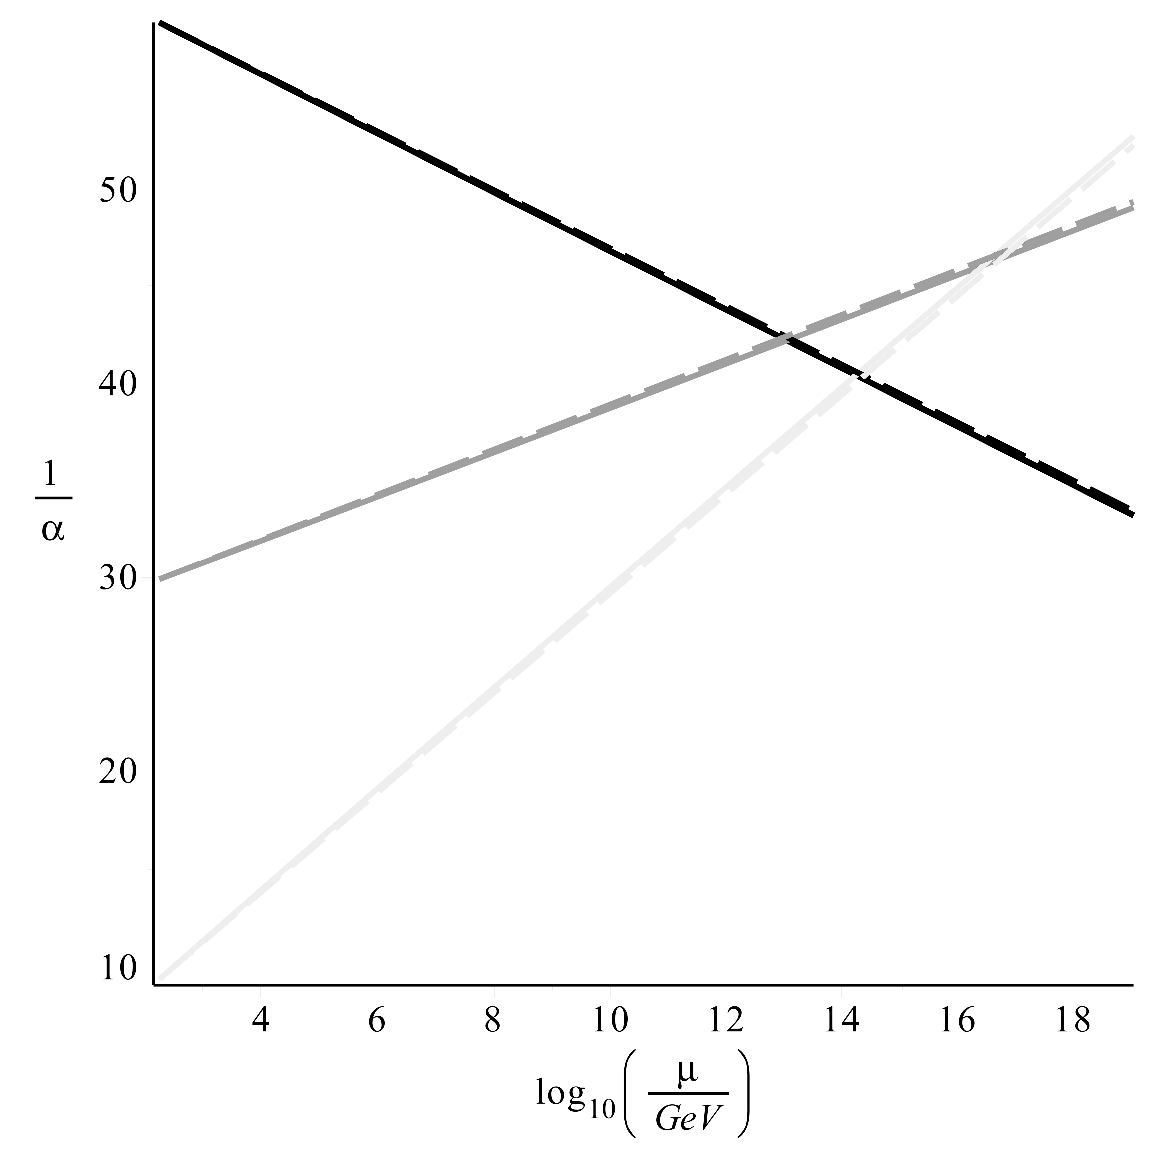
\includegraphics[width=.9\textwidth]{SPE_Lizzi/gaugerun-druk.pdf}
}
\caption{The running of the coupling constants of the three gauge interactions.}
\end{figure}
The boundary values at low energy are established experimentally, and the renormalization flow show that the nonabelian interactions proceed towards asymptotic freedom, while the abelian one climbs towards a Landau pole at incredibly high energies \formu{10^{53}}~{GeV}. The figure also show that the three interaction \emph{almost} meet at a single value at a scale around $10^{15}$~GeV. The lack of a unification point was one of the reasons for the falling out of fashion of GUT's, but it should be noted that some supersymmetric theory allow the unification point. It is however unlikely that the quantum field theory survives all the way to infinite energy, or at least to the Landau pole. We all believe that this running will be stopped by {```something''} at the Planck energy (mass), which is the energy equivalent of the Planck's lenght $\ell$ of ~\eqref{ell}:
\be
M_p=\sqrt{\frac{\hbar c}G}\simeq
10^{19}~\mathrm{GeV}.
\ee
 This unknown something we call \emph{quantum gravity}. At this scale there will certainly be some new physics, because it will be impossible to ignore gravitational effects.

We take the point of view that in the Planckian energy regime there is a fundamental change of the degrees of freedom of spacetime. Like what happens in a phase transition. One useful tool to describe this is new physics is \emph{Noncommutative Spectral Geometry}\footnote{For personal reviews in increasing level of detail see \parencite{Vilasiproc, Corfuproc, DevastatoLizziKurkov}.}. In this framework geometry is algebrized, the topological, metric and gauge aspects of the theory are encoded in a $C^*$-algebra acting on the Hilbert space of physical fermions, a generalised Dirac operator containing the information of the masses (Yukawa couplings) and of the metric, and chirality and charge conjugation. The model is successfully applied to the standard model and it has some predictive power \parencite{AC2M2, ColdPlay, CCvS, Grandproc, Aydemir:2015nfa, Walterbook}.


The metric and geometric properties are encoded in the (generalized) Dirac operator $D$ which fixes the background, he action is then an expansion around this background. Here we must make a ``confession''. The model is Euclidean and it consider a compact space. The latter is usually considered a minor problem, but the infrared frontier may have surprises, see for example the recent interest in it in \parencite{Strominger, eomconstraints, scent}. The issue of a Lorentzian, or at least causal, version of this noncommutative geometry is under active investigation, a partial list of references is \parencite{Dungen:2015pca, Bizi:2016lbv, Franco:2012er, Franco:2013gxa, Franco:2015qra, DAndrea:2016hyl, Kurkov:2017wmx, Devastato:2017rlo, Bochniak:2018ucd, Aydemir:2019txw}.


The eigenvalues of the Dirac operator on a curved spacetime are diffeomorphism-invariant functions
of the geometry. They form an infinite set of observables for general relativity and are therefore well suited to investigate the structure of spacetime. The interaction among fields is described by the \emph{Spectral Action:}
\be
S=\Tr\chi\left(\frac{D_A^2}{\Lambda^2}\right), \label{bosonicspectralact}
\ee
where $\chi$ is a cutoff function, which we may take to be a decreasing exponential or a smoothened version of the characteristic function of the interval, $\Lambda$ is a cutoff scale without which the trace would diverge. $D_A=D+A$ is a fluctuation of the Dirac operator, $A$ being a connection one-form built from $D$ as $A=\sum_i a_i[D,b_i]$ with $a_i,b_i$ elements of the algebra, the fluctuations are ultimately the variables, the fields of the action. the general ideas have a broader scope.  The presence of $\Lambda$ causes only a finite number of eigenvalues of $D_A$ to contribute, a finite number of modes. Finite mode regularization, based on the spectrum of the wave operator, was introduced in QCD \parencite{AndrianovBonora1, AndrianovBonora2, Fujikawabook}.

The bosonic spectral action can be seen as a consequence of the spectral cutoff \parencite{Andrianov:2010nr,Andrianov:2011bc,Kurkov:2012dn}, for description of Weyl anomaly and also phenomena of induced Sakharov Gravity \parencite{Sakharov} and cosmological inflation \parencite{Kurkov:2013gma}. It can also be seen as a zeta function calculated in zero \parencite{zeta}. The zeta-spectral action opens an intriguing opportunity to give a classically scale invariant formulation of the spectral action approach, where all the scales are generated dynamically.  Various mechanisms of scale generation were considered in both gravitational (Sakharov) or scalar fields sectors \parencite{ripples}. An enhanced role of the spectrum of the Dirac operator goes  far beyond the scope of spectral action. A simple analysis of the spectrum of the \emph{free} Dirac operator allows to arrive to a correct relation between three and four dimensional parity anomalies in gauge \parencite{Kurkov:2017cdz} and gravitational \parencite{Kurkov:2018pjw} sectors.





The spectral action can be expanded in powers of $\Lambda^{-1}$ using standard heat kernel techniques.
In this framework it is possible to describe the action of the standard model.
One has to choose as $D$ operator a tensorial combination of the usual Dirac operator on a~curved background  $\slashed\nabla$ and a matrix containing the fermionic parameters of the standard model (Yukawa couplings and mixings), acting on the product of spinors on spacetime times the fermionic degrees of freedom. In this way one ``saves'' one parameter, and can predict the mass of the Higgs. The original prediction was 170~GeV, which is not a bad result considering that the theory is basically based on pure mathematical requirements. When it was found at 125~GeV it was realized that the model had to be refined (right handed neutrinos play a central role) to make it compatible with present experiments. 
we will not dwell further on the Higgs issue, and concentrate on the role of the spectral action for spacetime.

Technically \parencite{manual} the bosonic spectral action is a~sum of residues and can
be expanded in a power series in terms of $\Lambda^{-1}$ as
\be
S_B=\sum_n f_n\, a_n(D_A^2/\Lambda^2),
\ee
where the $f_n$ are the momenta of $\chi$
\begin{eqnarray}
f_0&=&\int_0^\infty \dd x\, x  \chi(x)\nonumber\\
f_2&=&\int_0^\infty \dd x\,   \chi(x)\nonumber\\
f_{2n+4}&=&(-1)^n \del^n_x \chi(x)\bigg|_{x=0} \ \ n\geq 0.
\end{eqnarray}
The $a_n$ are the Seeley-de Witt coefficients which vanish for $n$
odd. For $D_A^2$ of the form
\be
D_A^2=-(g^{\mu\nu}\del_\mu\del_\nu\mathbb I+\alpha^\mu\del_\mu+\beta).
\ee
Defining (in term of a generalized spin connection containing also the gauge
fields)
\begin{eqnarray}
\omega_\mu&=&\frac12 g_{\mu\nu}\left(\alpha^\nu+g^{\sigma\rho} \Gamma^\nu_{\sigma\rho}\mathbb I\right),\nonumber\\
\Omega_{\mu\nu}&=&\del_\mu\omega_\nu-\del_\nu\omega_\mu+[\omega_\mu,\omega_\nu],\nonumber\\
E&=&\beta-g^{\mu\nu}\left(\del_\mu\omega_\nu+\omega_\mu\omega_\nu-\Gamma^\rho_{\mu\nu}\omega_\rho\right),
\end{eqnarray}
then%
%\noindent\resizebox{.87\textwidth}{!}{
%	\begin{minipage}{\linewidth}
%\begin{eqnarray*}
%a_0&=&\frac{\Lambda^4}{16\pi^2}\int\dd x^4 \sqrt{g}
%\tr\mathbb I_F,\nonumber\\
%a_2&=&\frac{\Lambda^2}{16\pi^2}\int\dd x^4 \sqrt{g}
%\tr\left(-\frac R6+E\right),\nonumber\\
%a_4&=&\frac{1}{16\pi^2}\frac{1}{360}\int\dd x^4 \sqrt{g}
%\tr(-12\nabla^\mu\nabla_\mu R +5R^2-2R_{\mu\nu}R^{\mu\nu},\nonumber\\
%&&+2R_{\mu\nu\sigma\rho}R^{\mu\nu\sigma\rho}-60RE+180E^2+60\nabla^\mu\nabla_\mu
%E+30\Omega_{\mu\nu}\Omega^{\mu\nu}), 
%\end{eqnarray*}
%\end{minipage}
%}
%\vspace*{-1.1
%	\normalbaselineskip}
%\begin{eqnarray}
%\end{eqnarray}\label{spectralcoeff}%label do eq wyzej, ofc
%
%\vspace*{-1\baselineskip}
\begin{eqnarray}
			a_0&=&\frac{\Lambda^4}{16\pi^2}\int\dd x^4 \sqrt{g}
			\tr\mathbb I_F,\nonumber\\
			a_2&=&\frac{\Lambda^2}{16\pi^2}\int\dd x^4 \sqrt{g}
			\tr\left(-\frac R6+E\right),\nonumber\\
			a_4&=&\frac{1}{16\pi^2}\frac{1}{360}\int\dd x^4 \sqrt{g}
			\tr(-12\nabla^\mu\nabla_\mu R +5R^2-2R_{\mu\nu}R^{\mu\nu},\nonumber\\
			&&+2R_{\mu\nu\sigma\rho}R^{\mu\nu\sigma\rho}-60RE+180E^2\nonumber\\
			&&+60\nabla^\mu\nabla_\mu
			E+30\Omega_{\mu\nu}\Omega^{\mu\nu}),
\end{eqnarray}\label{spectralcoeff}
${\rm tr}$ is the trace over the inner indices of the finite algebra
$\mathcal A_F$ and  $\Omega$ and $E$  contain the gauge
degrees of freedom including the gauge stress energy tensors and the
Higgs, which is given by the inner fluctuations of $D$

Let me analyse the role of $\Lambda$. Without it, the trace in \eqref{bosonicspectralact} would diverge. Field theory cannot be valid at all scales. It is itself a theory which emerges from a yet unknown quantum gravity.
This points to a geometry in which the spectrum of operators like Dirac operator are  {truncated}, i.e.\ the eigenvalues ``saturate'' at $\Lambda$, which appears as the top scale at which one can use QFT. One may identify this scale with $\ell$, but it might be different (even lower, at the unification scale). Apart from the spectral action, truncation on a matrix basis is a common tool in noncommutative geometry \parencite{matrixreview}.


Consider the eigenvectors $\ket{n}$ of \formu{D_A} in increasing order of the respective eigenvalue \formu{\lambda_n}. \formu{D=\sum_0^\infty\ket n \lambda_n \bra n}. Define \formu N as the maximum value for which \formu{\lambda_n\leq\Lambda}.  This defines the truncated Dirac operator 
\be
D_\Lambda=\sum_0^N\ket n \lambda_n \bra n+\sum_N^\infty\ket n \Lambda \bra n. 
\ee
We are effectively saturating the operator at a scale \formu{\Lambda}.

Given a space with a Dirac operator one can define a distance~\cite{Connesbook} between states of the algebra of functions, in particular points are (pure) states and the distance is:
\be d(x,y)=\sup_{\|[D,f]\|\leq1}\left| f(x)-f(y)\right|.\ee
It is possible possible to prove \parencite{DAndrea:2013rix}
 that using \formu{D_\Lambda}   the distance among points is infinite. In general for a bounded Dirac operator of norm \formu{\Lambda} then \formu{d(x,y)>\Lambda^{-1}}, and to find states at finite distance one has to consider ``extended'' points, such as coherent states.



We will try to infer, from a field theory which we know works at ``low'' energy, the behaviour of it at scales which are beyond a~cutoff. We are of course on dangerous grounds, we are stretching a~theory beyond it natural realm of validity. We are assuming that the scale of renormalization has a physical meaning, and is not a device to regularize the infinities of the theory, and we are using an action which, while is capable to reproduce some features of the standard model, is not really equipped to quantize gravity.
Having done the disclaimer let me proceed. We will investigate the spectral action in the limit of \emph{high momenta} using an expansion which sums up all derivatives. We will follow closely our paper with Vassilevich and Kurkov \parencite*{Kuliva}.

Consider the generic fermionic partition function:
\formula{Z = \int [d\bar\psi][d\psi]e^{-\langle \psi | D |\psi\rangle \ } \stackrel{\mbox{\tiny formally}}{=}  \det{ D} .} 
 The equality is formal because the expression is divergent, and has to be regularized, and the natural choice for us is to chose $D_\Lambda$. The considerations are nevertheless more general. One can study the renormalization flow, and note that the measure is not invariant under scale transformation, giving rise to a potential anomaly \parencite{Andrianov:2010nr, Andrianov:2011bc}.
The induced term by the flow, which takes care of the anomaly, turn out to be exactly the spectral action.

We will make the working hypothesis that \formu{\Lambda} has a physical meaning, it is a scale indicating a phase transition, and we can try to infer some properties of the phase above \formu{\Lambda} studying the high energy limit of the action with the cutoff. We will use field theory to do this, and will find, in the end, that at high momentum Green's function, the inverse of \formu{D_\Lambda}, effectively is the identity in momentum space. More precisely, we will expand the action around high momenta, rather than low ones, as is usually done. let us see this in greater detail considering the bosonic sector.



Usually probes are bosons, hence let us consider the expansion of the spectral action in the high momentum limit.
This has been made by Barvinsky and Vilkovisky \parencite*{Barvinsky:1990up} who were able to sum all derivatives (for a decreasing exponential cutoff function):

\noindent\resizebox{.82\textwidth}{!}{
	\begin{minipage}{\linewidth}
\begin{eqnarray*}
\Tr{\exp{\left(-\frac{D^2}{\Lambda^2 }\right)}} 
&\simeq&\frac{\Lambda^4}{(4\pi )^2} \int d^4x \sqrt{g}\, {\rm tr}\, \left[ 1 + \Lambda^{-2}P + \right. \nonumber\\
&&\Lambda^{-4}\left( 
R_{\mu\nu} c_1\left(-\frac{\nabla^2}{\Lambda^2}\right) R^{\mu\nu} + Rc_2\left(-\frac{\nabla^2}{\Lambda^2}\right)R  +\right.\nonumber\\
&&\left. Pc_3\left(-\frac{\nabla^2}{\Lambda^2}\right)R +Pc_4\left(-\frac{\nabla^2}{\Lambda^2}\right) P 
+ \Omega_{\mu\nu} c_5\left(-\frac{\nabla^2}{\Lambda^2}\right)\Omega^{\mu\nu}
\bigr) \right]  \nonumber\\
&&+ O(R^3,\Omega^3,E^3) ,
\end{eqnarray*}
\end{minipage}
}
\vspace*{-1.39\baselineskip}
\begin{eqnarray}
\end{eqnarray}%nr eq wyzej, ofc
where \formu{P= E+\tfrac 16 R} and  \formu{c_1,\ldots,c_5} are known functions, high momenta asymptotic of form factor which can be calculated and are
\bea
c_1(\xi) &\simeq& \frac{1}{6}\,{\xi}^{-1}-{\xi}^{-2} + O \left( {\xi}^
{-3} \right), \nonumber \\
c_2(\xi) &\simeq& -\frac{1}{18}\,{\xi}^{-1}+\frac{2}{9}\,{\xi}^{-2} + O \left( {\xi}^{-3}
 \right),  \nonumber \\
 c_3(\xi) &\simeq& -\frac{1}{3}\,{\xi}^{-1}+\frac{4}{3}\,{\xi}^{-2} + O
 \left( {\xi}^{-3} \right), \nonumber\\
 c_4(\xi) &\simeq& {\xi}^{-1}+2\,{\xi}^{-2} + O \left( {\xi}^{-3}
 \right)  \nonumber\\
 c_5(\xi) &\simeq& \frac{1}{2}\,{\xi}^{-1}-{\xi}^{-2} + O \left( {\xi}
^{-3} \right).
\eea

Let us first discuss the usual case (no truncation). Consider a Dirac operator containing just the relevant aspects, i.e. a bosonic fields and the fluctuations of the metric.
\formula{
\slashed{D}=i\gamma^\mu \nabla_\mu + \gamma_5 \phi= i\gamma^\mu (\del_\mu+\omega_\mu + iA_
\mu) +\gamma_5 \phi,\label{sD}}
with \formu{\omega_\mu} the Levi-Civita connection and  \formu{g_{\mu\nu}=\delta_{\mu\nu}+h_{\mu\nu}}. The field $\phi$ for the time being is a generic scalar field. When the Dirac operator becomes the one of the standard model it may be indetified with the Higgs. It is now possible to perform the B-V expansion to get the expression for the high energy spectral action:
\noindent\resizebox{.95\textwidth}{!}{
	\begin{minipage}{\linewidth}
\begin{equation*}
S_B\simeq  
\frac {\Lambda^4}{(4\pi )^2} \int d^4x \left[ -\tfrac 32  h_{\mu\nu}h_{\mu\nu}
+8 \phi \frac 1{-\partial^2} \phi + 8 F_{\mu\nu} \frac 1{(-\partial^2)^2} F_{\mu\nu} \right].
\end{equation*}
	\end{minipage}
}
\vspace*{-1.9\baselineskip}
\begin{equation}
\end{equation}
In order to understand the meaning of this action let us remind how we obtain the propagation of particles and fields and correlation of points in usual QFT with action:
\formula{
S[J,\varphi] = \int d^4 x \left[\frac12\varphi(x)\left(\partial^2 + m^2 \right)\varphi(x)  - J(x)\varphi(x) \right].}
To this correspond the equation of motion
\formula{
\left(\partial^2 + m^2 \right)\varphi(y)  = J(y),}
and the Green's function \formu{G(x-y)} which ``propagates'' the source: 
\formula{
\varphi_J(x)=\int d^4y J(y) G(x-y).}
In the momentum representation we have:
\bea
\varphi(x) &=&  \frac{1}{\left(2\pi\right)^2} \int d^4 k ~e^{ikx} ~ \hat{\varphi}(k). \nonumber\\
J(x) &=& \frac{1}{\left(2\pi\right)^2} \int d^4 k ~e^{ikx} ~ \hat{J}(k),\nonumber\\
G(x-y) &=& \frac{1}{\left(2\pi\right)^2} \int d^4 k ~e^{ik(x-y)} ~ \hat{G}(k),
\eea
and the propagator is
\formula{G(k) = \frac1{\left(k^2+m^2\right)}.}
The field at a point depends on the value of field in nearby points, and the points ``talk'' to each other exchanging virtual particles.




In the general case of a generic boson \formu{\varphi}, the Higgs, an intermediate vector boson or the graviton and \formu{F(\del^2)} the appropriate wave operator, a generalised Laplacian
\formula{
S[J,\phi]=\int d^4x \left(\frac12 \varphi(x) F(\del^2) \varphi(x) -J(x) \varphi(x)\right).\,}
In this case the equation of motion is
\be
F(\del^2)\phi(x)=J(x)\label{eom},
\ee
giving
\formula{
G=\frac1{F(\del^2)}\ , \ \ G(k)=\frac1{F(-k^2)}\ , }
and
the cutoff is telling us that\footnote{Note that with our signature, at low momentum $F(-k^2)=k^2+m^2$. There are some imprecise statements in the original paper \parencite{Kuliva}.}

\noindent\resizebox{.95\textwidth}{!}{
	\begin{minipage}{\linewidth}
		\begin{equation*}
\varphi_J(x)=\int d^4y J(y) G(x-y)=\frac1{(2\pi)^4}\int d^4k e^{ikx}J(k)\frac1{F(-k^2)} .
		\end{equation*}
	\end{minipage}
}
\vspace*{-1.75\baselineskip}
\begin{equation}
\end{equation}
The short distance behaviour is given by the limit \formu{k\to\infty}.

Consider \formu{J(k)\neq 0} for \formu{|k^2|\in[K^2,K^2+\delta k^2]}, with \formu{K^2} very large. 
Then the propagated field becomes:

\noindent\resizebox{.99\textwidth}{!}{
	\begin{minipage}{\linewidth}
		\begin{equation*}
\varphi_J(x) \xrightarrow[{{\scriptstyle K\to\infty}}]{}
\left\{\begin{array}{ll} \frac1{(2\pi)^4}\int d^4k e^{ikx} J(k) k^2=(-\del^2)J(x)  & \mbox{\small for scalars}  \\[-6pt]
&\mbox{\small and vectors,}\\
\frac1{(2\pi)^4}\int d^4k e^{ikx} J(k) =J(x)  & \mbox{\small for gravitons.} 
\end{array}
\right .
\end{equation*}
\end{minipage}
}
\vspace*{-.7\baselineskip}
\begin{equation}
\end{equation}
This  corresponds to a limit of the Green's function in position space
\formula{
G(x-y)\propto\left\{\begin{array}{ll} (-\del^2)\delta\left(x-y\right)   & \mbox{for scalars and vectors,}  \\
\delta\left(x-y\right)  & \mbox{for gravitons.} 
\end{array}
\right. }
The correlation vanishes for noncoinciding points, heuristically, nearby points ``do not talk to each other''.
This is a limiting behaviour, we are inferring the behaviour at high energy extrapolating from low energy expanding around infinity. It is a little like a fish attempting to know what is beyond the surface of the water!
One has to take it as a general indication that the presence of a physical cutoff scale in momenta leads to a ``non geometric phase'' in which the concept of point ceases to have meaning, possibly described by a noncommutative geometry.

Note that throughout this discussion spacetime has been left unaltered. We just imposed the cutoff and used standard techniques and interpretations. Hence we did not touch upon points in this discussion.  Points might still be there, but they are uncorrelated at very high energy. Somehow their meaning is lost, since they are not operatively correlated. In our opinion this indicates a phase transition for which the locality order parameter (position) is not present anymore.
 But it also gives us the indication that quantum gravity must be a~theory in which points are not the relevant entity.
This is consistent with several other work, which in different contexts, and using different techniques, find similar phenomena. For example asymptotic silence whereby, near gravitational singularities, light cones collapse into lines, so that again nearby points cannot communicate, or ``hear each other''.  This is but an extreme version of dimensional reduction, a recent good review is \parencite{Carlip}. Also the concept of event becomes debatable in versions of $\kappa$-Minkoski, giving rise to the concept of relative locality \parencite{relaloc} and the fact that localization is observer dependent \parencite{LMM}.





According to the interpretation given in this review we are like the deep water fish trying to understand what goes on above his ceiling.
He knows that pressure decreases as he goes up. He can also infer some properties of a different states of matter by looking at bubbles which are creates near some ``high energy'' volcanic vents or when ``above'' there are storms, but he cannot naturally grasp the concept of air, or absence of water.
He will need a higher leap: quantum gravity. The hope is that this kind of considerations might help.

\paragraph{Acknowledgement}
I would like to thank Micha\l{} Heller and Micha\l{} Eckstein for organizing the meeting which gave me a chance to think with a more ``philosophical'' perspective. The whole experience was very stimulating and I enjoyed it very much. I thank Maxim Kurkov and the referees for a critical reading of the manuscript.
I am also grateful for the support of the INFN Iniziativa Specifica GeoSymQFT and Spanish
MINECO under project MDM-2014-0369 of ICCUB (Unidad de Excelencia `Maria de Maeztu') and  COST action \emph{QSPACE}.



\end{artengenv}

%-------------------------------
  


\begin{artengenv}{Klaus Fredenhagen}
	{Independent quantum systems and the associativity of the product of quantum observables}
	{Independent quantum systems and the associativity\ldots}
	{Independent quantum systems and the associativity of the product of quantum observables}
	{II. Institut f\"ur Theoretische Physik Universit\"at Hamburg}
	{We start from the assumption that the real valued observables of a quantum system form a Jordan algebra which is equipped with a compatible Lie product characterizing infinitesimal symmetries,
		and ask whether two such systems can be considered as independent subsystems of a larger system. We show that this  is possible if and only if the associator of the Jordan product is a fixed multiple of the associator of the Lie product. In this case it is known that the two products can be combined to an associative product in the Jordan algebra or its complexification, depending on the sign of the multiple.}
	{quantum systems, quantum observables.}
	
	

\section{Introduction}
\lettrine[loversize=0.13,lines=2,lraise=-0.05,nindent=0em,findent=0.2pt]%
{I}{}n quantum theory, the (real valued) observables are self-adjoint elements of a complex associative involutive algebra. This structure is quite different from the classical case where the observables form a Poisson algebra, i.e. an algebra over the reals with a commutative and associative product  and a Lie product inducing derivations for the commutative product. 

As emphasized by Niklas Landsman in his book \parencite*{Landsman}, the structure in the quantum case can be formulated in an analogous way by equipping the selfadjoint part of the algebra with the Jordan product (i.e. $\frac12$ times the anticommutator) and a Lie product defined as $\frac{i}{\hbar}$ times the commutator.
Both products have a physical motivation quite similar to the classical case. In particular the induced derivations of the Jordan product by the Lie product are motivated by their interpretation as infinitesimal symmetries, and the Jacobi identity for the Lie product may be understood as a consistency condition on symmetries. Both products are non-associative, and the associator of the Jordan product is $\hbar^2/4$ times the associator of the Lie product. 

The question we want to analyze in this paper is whether the latter relation between the associators can be physically motivated. Mathematically it implies that both products can be combined to an associative product in a complexification of the algebra.
This algebra has an antilinear involution, and its self-adjoint part is the original Jordan algebra with the Lie product given in terms of the commutator.    

To answer this question we add the requirement that independent physical systems can be considered as parts of a larger system, such that the properties of the subsystems are not influenced by the embedding into the larger system. 
We show that the validity of the Jacobi identity in the composed system implies that the associators of the Jordan products are proportional to the associators of the Lie product, with a proportionality constant which is independent  of the system. If the constant is positive, one obtains an associative product in the complexified algebras, and the composed system arises as the self-adjoint part of the tensor product of the associative algebras. 

The idea to derive the associative product of quantum physics from the composibility of systems was first discussed in the paper of Grgin and Petersen \parencite*{P} and reconsidered more recently by Kapustin \parencite*{K} and Moldoveanu \parencite*{M}. 
 A related but independent result applying to the infinite dimensional case can be found in \parencite{H}, see also the book  \parencite{HS}. Contrary to these works we do not make any \textit{a priori} assumptions on the way the larger system can be built from the subsystems.
 
 
 
 
 
 
%%%%%%%%%%%%%%%%%
\section{Jordan-Lie algebras}
\lettrine[loversize=0.13,lines=2,lraise=-0.05,nindent=0em,findent=0.2pt]%
{A}{} Jordan algebra is a real vector space $A$ equipped with a commutative product 
\renewcommand{\c}{\circ}
$\c$, i.e. a bilinear map
\[A\times A\to A, (a,b)\mapsto a\c b\]
with $a\c b=b\c a$.
This product is not necessarily associative, instead only the weaker relation 
\be
\label{Jordan}
(a^2\c b)\c a=a^2\c(b\c a)
\ee
holds, where $a^2=a\c a$. Jordan introduced this concept in order to describe the structure one can expect for quantum observables. Indeed, the linear structure may be motivated by Ehrenfest's Theorem stating that expectation values add as in classical physics \parencite[see e.g.][]{Arodz}; labeling of measurement results in terms of real numbers may be redefined by applying a mapping $\RR\to\RR$, so in particular squares of observables can be defined, and a commutative product can be introduced by
\[a\c b\doteq\frac12((a+b)^2-a^2-b^2)\ .\] 
The condition \eqref{Jordan} follows from the requirement that powers are well defined,
\[a^n\circ a^m=a^{n+m}\]
where $a^1=a$, $a^{n+1}=a^n\c a$, under the additional positivity condition
\be\label{positiv}
\sum a_i^2=0\ \Rightarrow a_i=0\ .
\ee
(See \parencite{JNW}; such a Jordan algebra is called formally real.)
Finite dimensional Jordan algebras can be classified. Besides the standard case of selfadjoint subalgebras of associative involutive algebras over $\RR,\CC$ or 
$\mathbb{H}$ (the quaternions) one has a few exceptional cases. We only consider unital Jordan algebras, i.e. there is an element $1\in A$ which satisfies the relation
\be\label{unit}1\c a=a\forall a\in A\ .\ee 
For finite dimensional Jordan algebras the existence of the unit is a consequence of the positivity condition \eqref{positiv}.

In addition to the Jordan product of observables one has in quantum theory a Lie product in terms of commutators which describes the dual role of observables as generators of infinitesimal symmetries. The standard example is Heisenberg's equation of motion
characterizing the time evolution, and it corresponds directly to the Poisson bracket of classical physics, as first observed by Dirac. The arising structure has been analyzed by Landsman \parencite*{Landsman}. He defines a Jordan-Lie algebra as a Jordan algebra $(A,\c)$ with a Lie product, i.e. a bilinear map   
\[
A\times A\to A\ ,\ (a,b)\mapsto [a,b]
\]
which is antisymmetric
\[ [a,b]=-[b,a]\]
and satisfies the Jacobi identity
\be\label{Jacobi}[[a,b],c]+[[b,c],a]+[[c,a],b]=0\ .\ee
The Lie product is related to the Jordan product by two relations. The first is the Leibniz rule
\be\label{Leibniz}[a\c b,c]=a\c[b,c]+[a,c]\c c\ .\ee
This rule is motivated by the interpretation of the map $A\ni a\mapsto[a,c]$ as an infinitesimal symmetry.
The second relation involves the associators. 
Denote the associator of the Jordan product by
\[[a,b,c]\doteq(a\c b)\c c-a\c(b\c c)\]
and the associator of the Lie product by
\[[[a,b,c]]\doteq[[a,b],c]-[a,[b,c]]\equiv[[a,c],b]\ .\]
Then the relation is
\be\label{ass}[a,b,c]=\frac{\hbar^2}{4}[[a,b,c]]\ .\ee
\newcommand{\ot}{\otimes}
One then can introduce a product $\cdot$ on the complexification $A\ot\CC$ of $A$, by
\be\label{complex} (a\ot z)\cdot( b\ot w)=(a\c b)\ot zw+[a,b]\ot\frac{i\hbar zw}{2},\ee
which turns out to be associative due to \eqref{ass}. One thus obtains the standard structure of the algebra of quantum observables.
It remains open whether the relation \eqref{ass} between the two associators has a physical interpretation.

We therefore introduce the concept of a q-algebra where the condition \eqref{ass} is not imposed. We also do not require the Jordan condition \eqref{Jordan} and the positivity relation \eqref{positiv}
\begin{definition-fred}
A q-algebra is a real vector space equipped with a commutative product $\c$ and an antisymmetric product $[,]$. It contains a unit for the commutative product \eqref{unit} and satisfies the Jacobi identity \eqref{Jacobi} and the Leibniz rule \eqref{Leibniz}.
\end{definition-fred}


%%%%%%%%%%%%
\section{Independent subsystems}
Let $A,B$ and $C$ be q-algebras.
To model the requirement that $A$ and $B$ represent independent subsystems of the larger system represented by $C$ we require the following relations:
\begin{definition-fred}\label{independent}
Let $\alpha:A\to C$ and $\beta:B\to C$ be monomorphisms of q-algebras. The pair $(\alpha,\beta)$ is called an embedding of independent subsystems if the following conditions are satisfied: 
\begin{enumerate}\label{composition}
\item the map
\[A\times B\ni(a,b)\to \alpha(a)\c\beta(b)\in C \]
extends to an injective linear map  $\alpha\ot\beta:A\ot B\to C$.
\item the infinitesimal symmetries implemented by elements of $A$ act trivially on $B$ and vice versa,
 \be\label{loc1}[\alpha(a),\beta(b)]=0 \ \forall a\in A,b\in B, \ \ee
\item the $\c$-product with an observable of one of the subsystems does not affect the $\c$-product in the other subsystem (the observables from $A$ are compatible with the observables from $B$ in the context of Jordan algebras \parencite{HS})
\be\label{loc2}(\alpha(a)\c(\alpha(a')\c\beta(b))=\alpha(a\c a')\c\beta(b)\ , (\alpha(a)\c\beta(b))\c\beta(b')=\alpha(a)\c\beta(b\c b')\ ,\ee
%\item $C$ is generated by $\alpha(A)$ and $\beta(B)$.
\end{enumerate}
\end{definition-fred}
In the following we omit the symbols $\alpha$ and $\beta$ by identifying $A$ and $B$ with their embeddings in $C$. Moreover, we delete the symbol $\c$ for the commutative product and replace it by juxtaposition. 
We first determine the antisymmetric product in the image $C_0$ of $\alpha\ot\beta$:
\begin{lemma-fred}
The antisymmetric product in $C_0$ is given by
\be\label{LieC}[ab,a'b']=[a,a'](bb')+(aa')[b,b']\ , a,a'\in A,\ b,b'\in B \ .\ee
In particular, $C_0$ is closed under the antisymmetric product.
\end{lemma-fred}
\begin{proof}
By \eqref{Leibniz}, \eqref{loc1} and \eqref{loc2} we have
\begin{equation*}
\begin{split}
[ab,a'b']=a[b,a'b']+[a,a'b']b=a(a'[b,b'])+([a,a']b')b\\
=[a,a'](b'b)+(aa')[b,b']\ .
\end{split}
\end{equation*}
\end{proof}
In the next step we analyze the consequences of the Jacobi identity within $C_0$.
%By assumption, the antisymmetric product in $C_0$ satisfies the Jacobi identity.
We compute the second antisymmetric product, with $a_i\in A,b_i\in B,i=1,2,3$, 
\[[[a_1b_1,a_2b_2],a_3b_3]=[[a_1,a_2]b_1b_2+a_1a_2[b_1,b_2],a_3b_3]\]
\[=[[a_1,a_2],a_3](b_1b_2)b_3+(a_1a_2)a_3[[b_1,b_2],b_3]\]
\be\label{Jac1}+[a_1,a_2]a_3[b_1b_2,b_3]+[a_1a_2,a_3][b_1,b_2]b_3\ .\ee
In the last 2 terms we apply the derivation property \eqref{Leibniz} and obtain 4 terms,
\[[a_1,a_2]a_3[b_1b_2,b_3]+[a_1a_2,a_3][b_1,b_2]b_3\]
\[=[a_1,a_2]a_3b_1[b_2,b_3]+[a_1,a_2]a_3[b_1,b_2]b_3\]
\[+a_1[a_2,a_3][b_1,b_2]b_3+[a_1,a_3]a_2[b_1,b_2]b_3\ .\]
If we perform a cyclic sum over the indices we see that the 1\textsuperscript{st} and the 4\textsuperscript{th} term cancel, and also the 2\textsuperscript{nd} and 3\textsuperscript{rd} term. 

Thus for the Jacobi identity only the first 2 terms in \eqref{Jac1}
contribute. We use the Jacobi identities in $A$ and $B$,
\[[[a_1,a_2],a_3]=-[[a_2,a_3],a_1]-[[a_3,a_1],a_2]\ ,\]
\[[[b_1,b_2],b_3]=- [[b_2,b_3],b_1]- [[b_3,b_1],b_2]\ .\]
The Jacobi identity in $C$ then amounts to the relation
\[0=[[a_2,a_3],a_1]((b_2b_3)b_1-(b_1b_2)b_3)\]
\[+[[a_3,a_1],a_2](b_3b_1)b_2-(b_1b_2)b_3)+(a\leftrightarrow b))\]
\[\equiv [[a_2,a_1,a_3]][b_3,b_2,b_1]+[[a_3,a_2,a_1]][b_3,b_1,b_2]+(a\leftrightarrow b)).\]
To simplify this expression we choose $a_3=a_1$. Then both associators $[[a_3,a_2,a_1]]$ and $[a_3,a_2,a_1]$ vanish, and we obtain the relation
\be\label{Jac2}[[a_2,a_1,a_1]][b_3,b_2,b_1]+[a_2,a_1,a_1][[b_3,b_2,b_1]]=0\ .\ee
We want to exclude the possibility that $[[a_2,a_1,a_1]]=0\forall a_1,a_2\in A$. If all these quantities would vanish, the associator for the antisymmetric product would be totally antisymmetric and hence had to vanish because of the Jacobi identity. We therefore require that the associator of the antisymmetric product in $A$ is nonvanishing. 
%But then there are also elements $a,a''\in A$ with $[[a,a,a'']]\not=0$.
%Namely assume that $[a,a']\not=0$ but $[[a,a,a']]=0=[[a,a'],a]$. Then we choose $a''=(a'^2)$, obtain by \eqref{Leibniz}
%\be\label{Jac3}[[a,a,(a')^2]]=[[a,(a')^2],a]=[2a'[a,a'],a]=-2[a,a']^2\ ,\ee
%and conclude from \eqref{positiv} that $[a,a']^2\not=0$.   
Since $C_0$ is as a vector space isomorphic to $A\ot B$,
%assume that the linear space generated by products of the form $ab$, $a\in,b\in B$ is isomorphic to the tensor product $A\otimes  B$ of the two vector spaces. Then
%if $[[a_2,a_1,a_2^2]]\not=0$ for some $a_1,a_2\in A$ 
we find the relation
\be[b_3,b_2,b_1]=\lambda[[b_3,b_2,b_1]]\label{ass2}\ee
for some $\lambda \in \RR$.

Finally, we determine the symmetric product in $C_0$, under the assumption that the associator relation \eqref{ass2} holds within $C$. By the independence of the embeddings we have
\[(ab)b'=a(bb')\text{ and }a(a'b)=(aa')b. \]
We now compute $(ab)(a'b')$. We have by the definition of the associator
\[(ab)(a'b')=((ab)a')b'-[ab,a',b]\ .\]
We apply \eqref{loc2} twice and obtain
\[((ab)a')b'=(a'(ab))b'=((aa')b)b'=(aa')(bb')\ .\]
Thus, due to the relation \eqref{ass2} between the associators,
\[[ab,a',b']=\lambda[[ab,b'],a']=\lambda [a[b,b'],a']=\lambda[a,a'][b,b']\ .\]
We therefore arrive at the formula for the symmetric product
\be\label{JordanC}(ab)(a'b')=(aa')(bb')-\lambda[a,a'][b,b']\ .\ee
We conclude that $C_0$ is also closed under the symmetric product. %Since $C$ is generated by $A$ and $B$, it coincides with $C_0$.

An embedding of $A$ and $B$ can be constructed if both satisfy \eqref{ass2} with the same $\lambda$. Let $A\ot B$ be the tensor product of the vector spaces $A$ and $B$. We introduce a symmetric product
\[(a\ot b)\circ(a'\ot b')=a a'\ot b b'-\lambda[a,a']\ot[b,b']\]
and an antisymmetric product
\[[a\ot b,a'\ot b']=[a,a']\ot b b'+a a'\ot[b,b']\]
and obtain a q-algebra $A\ot_\lambda B$ together with maps $\alpha:A\to A\ot B,\ a\mapsto a\ot 1$, $\beta:B\to A\ot B,\ b\mapsto 1\ot b$ which satisfy the condition of an independent embedding.
Moreover, also the associators in $A\ot_{\lambda}B$ satisfy the associator relation \eqref{ass2}.

We arrive at the following theorem:
\begin{theorem-fred}
Let $A,B$ be q-algebras with nontrivial associators for the antisymmetric products. Then an embedding as independent subsystems exists if and only if  the associators in $A$ and in $B$ are related by \eqref{ass2} with the same $\lambda$.
% and let $C=A\otimes_{\lambda}B$ be the tensor product of the vector spaces $A$ and $B$, equipped with the symmetric and the antisymmetric product defined above. 
%assume that the antisymmetric products of $A$ and $B$ do not vanish identically. Then there is some $\lambda\in\RR$ such that the associators in $A$ and $B$ are related by \eqref{ass}.
 Moreover, given any such embedding $(\alpha,\beta):A\times B\to C$ where $C$ also satisfies \eqref{ass2}, there is a unique injective homomorphism $\gamma:A\ot_{\lambda}B\to C$ with $\gamma(a\ot b)=\alpha(a)\c\beta(b),\ a\in A,\ b\in B$.
 \end{theorem-fred}
 \begin{proof}
 Assume that an independent embedding exists. Then, from \eqref{Jac2}, we conclude the relation \eqref{ass2} for $B$. The argument for $A$ follows analogously. If, on the other side, \eqref{ass2} holds for both $A$ and $B$, we 
 can construct $A\ot_{\lambda} B$ as an example for an independent embedding.
 Now let $(\alpha,\beta):A\times B\to C$ be any independent embedding. The map $\gamma$ given in the Theorem is by definion a linear monomorphism and preserves the unit.  From \eqref{JordanC} and \eqref{LieC} we then conclude that also both products are preserved, hence $\gamma$ is a monomorphism of q-algebras.   
 \end{proof}
% We can now compute the antisymmetric products of elements of the form $\alpha(a)\beta(b)$:
%\be
%[\alpha(a)\beta(b),\alpha(a')\beta(b')]=\alpha(a)[\beta(b),\alpha(a')\beta(b')]+[\alpha(a),\alpha(a')\beta(b')]\beta(b)
%\ee
%\[=\alpha(a)(\alpha(a')[\beta(b)),\beta(b')]+([\alpha(a),\alpha(a')]\beta(b))\beta(b')]\]
%\[=\alpha(aa')\beta([b,b'])+\alpha([a,a'])\beta(bb')\]
%In the following we identify the elements of $A$ and $B$ with their images in $C$.
%By assumption, the antisymmetric product in $C$ satisfies the Jacobi identity. We use this identity for elements of the form 
%\section{Jordan Product}





\section{The operator product}
Let $A$ be a q-algebra which satisfies the associator equality for some $\lambda\in\RR$. We distinguish three cases:
\begin{description}
\item[{$\lambda=0:$}]
In this case the $\c$-product of $A$ is associative, and we are in the situation of classical physics.
\item[{$\lambda<0:$}]
For $\lambda<0$ we can introduce in $A$ an associative noncommutative product by
\[a\bullet b=a\c b+\sqrt{|\lambda|}[a,b]\ .\]
The $\c$ product is then $\frac12$ times the anticommutator, and it is easy to see that also the condition \eqref{Jordan} for Jordan algebras is fulfilled. If $A$ is finite dimensional, the positivity condition \eqref{positiv} cannot be fulfilled for associative algebras \parencite{Braun}. It is likely that this remains true in the infinite dimensional case, but existent results use additional input, in particular the existence of a norm. See \parencite{Mc} for an overview.  
 
%It is questionable whether such an algebra can satisfy the positivity condition \eqref{positiv}.
\item[{$\lambda>0:$}]
For $\lambda >0$ we define a product in the complexification $A\ot \CC$ of $A$ as in \eqref{complex} with $\hbar=2\sqrt{\lambda}$ and an antilinear involution
\[(a\ot z)^*=a\ot\overline{z}\ .\]
$A$ is then the self-adjoint subspace of the complex associative  involutive algebra $A\ot\CC$, hence we obtain the well known structure of quantum theory.
\end{description}


\paragraph{Acknowledgement}
We thank Christoph Schweigert and Joao Barata for helpful discussions.






\end{artengenv}

\begin{artengenv}{Henryk Arod\'z}
	{Ehrenfest's Theorem Revisited}
	{Ehrenfest's Theorem Revisited}
	{Ehrenfest's Theorem Revisited}
	{Marian Smoluchowski Institute of Physics \\ Jagiellonian University, Krak\'ow\label{arodz-start}}
	{Historically, Ehrenfest's theorem \parencite*{ehr} is the first one which shows that classical physics can emerge from quantum physics as a kind of approximation. We recall the theorem in its original form, and we highlight its generalizations to the relativistic Dirac particle and to a particle with spin and izospin. We argue that aparent classicality of the macroscopic world can probably be explained within the framework of standard quantum mechanics.}
	{Ehrenfest's theorem, wave packets, quantum vs. classical world.}



%{\large Ehrenfest's Theorem Revisited\footnote{Article based on talk given at the 22\textsuperscript{th} Krak\'ow Methodological Conference ``Emergence of the Classical'', Krak\'ow, October 2018. }}




\section{Introduction}


\lettrine[loversize=0.13,lines=2,lraise=-0.05,nindent=0em,findent=0.2pt]%
{T}{}he principal aim of both classical and quantum mechanics is to describe motions of certain physical objects. Both theories can be very successfully applied to various physical objects, but the sets of these objects do not coincide. As is well known, classical mechanics gives wrong predictions when applied to microscopic objects such as atoms. On the other hand, it seems that quantum mechanics is capable to correctly describe motions of the elementary particles as well as motions of macroscopic bodies, hence it has a wider range of applicability. Nevertheless, there are phenomena description of which requires a theory still more general than quantum mechanics. For example, scattering of elementary particles can lead to creation or annihilation of particles---here quantum field theory is needed. Such a generalization of quantum mechanics to quantum field theory is well-known since the middle of 20\textsuperscript{th} century. There are still some problems with it, but the prevailing opinion is that they concern more its mathematical side than foundations. Another departure from standard quantum mechanics seems to be necessary when an elementary particle interacts with a very complex, perhaps even randomly fluctuating or unstable, environment. Understanding of this case is rather poor. To a certain degree the situation is analogous to the well known partition of classical electrodynamics into the theory of the electromagnetic field in vacuum and the electrodynamics of 
continua with constitutive relations and other additional ingredients. An effective quantum mechanics in continua is still 
under construction. 





 It turns out that classical mechanics can be derived from quantum mechanics as a kind of approximate theory. Such derivations are usually called classical limit of quantum mechanics. There exist several of them, including the discussed below Ehrenfest type classical limit, which dates back to \cite*{ehr}, and is likely the oldest one. Its main feature is that it links solutions of the pertinent fundamental evolution equations, which are the Schroedinger wave equation in quantum mechanics and the Newton equation of motion in classical mechanics. Other kinds of classical limits are carried out on more advanced levels of theory. For instance, one may derive from quantum mechanics the classical Hamilton-Jacobi equation \parencite[see, e.g.][chap.8, sec.34]{WKB}, the Lagrange formalism \parencite[see, e.g.][chap.1, sec.2]{pathint}, or distributions on phase space \parencite[see, e.g.][]{siegel,wignerdistr}.



Our main goal here is to recall the seminal paper \parencite{ehr}, and to show, using modern examples, how fruitful is the invented by Paul Ehrenfest method for deriving classical mechanics from quantum mechanics. It leads to very interesting extended versions of classical mechanics featuring, e.g., a non relativistic particle with spin and izospin, or a relativistic particle with spin, which all emerge from quantum mechanics. Furthermore, Ehrenfest's theorem provides a tantalizing suggestion that perhaps whole classical physics can be recovered as certain approximations to quantum theories. Considering wave packets, we find some arguments that corroborate this idea. 

 

The present article is addressed to audience wider than just theoretical physicists. Nevertheless, certain familiarity with basic equations of classical and quantum mechanics is assumed. 






The plan of the article is as follows. First, we briefly discuss description of states of a particle in quantum mechanics with emphasis on the so called wave packets. Section~3 
is devoted to the original form of Ehrenfest's theorem. In Section~4 we sketch a solution of the main problem with the Ehrenfest method: the lack of relativistic covariance. 
Next, in the Section~5 we discuss certain extension of that theorem, which leads to a less known example of classical mechanics of a point-like particle with spin and izospin. Section~6 contains remarks on applicability of quantum mechanics to macroscopic bodies, including a new argument for practical nonexistence of so called Schroedinger's cats. 












\section{Quantum states of a particle }



Classical mechanics and quantum mechanics address the same issue: description of motions of a set of particles. Such set could consists of just one particle, or a finite number of them. The restriction to finite number of particles is important, because otherwise one would have to use a field theory which is regarded as different from mechanics for several important reasons. Classical and quantum mechanics are structurally similar to each other in the sense that in both theories we introduce a space of states of the particle and we postulate an equation of motion. They differ in the form of equation of motion: in classical mechanics this can be, for example, the Newton equation, while in quantum mechanics the Schr\"odinger equation. Also
 the spaces of states are very different. For instance, for the simplest single, point-like particle it is six dimensional phase space in classical mechanics, and infinite dimensional Hilbert space in quantum mechanics. The different equations of motion, and different sets of measurable properties (called observables) for the same set of particles are possible because the spaces of states in classical and quantum mechanics are not identical. Therefore, we regard this latter difference as the most important one. 

In this article we consider the simplest particles, which we describe as elementary. Particles which possess constituents, for example, hadrons, nuclei, or atoms, are excluded. Physical incarnations of the elementary particles are, e.g. electrons, photons, quarks, or the Higgs particle. 

The term `point-like particle' used above is well justified only in classical mechanics. It refers to the fact that in the simplest case the state of a single particle at fixed time $t$ is given by the position and velocity of the particle. The position is represented by a point in the $R^3$ space. In quantum mechanics the complete description of the state of the particle at a given time $t$ is provided by a smooth wave function $\psi(\vec{x}, t)$ defined on the $R^3$ space.\footnote{For simplicity, we consider here only so called pure states, omitting more general mixed states.} 
There is no reason to relate such a quantum particle with a material point moving in the space. Rather, it should better be pictured as a cloud of matter of a very special kind, which is present at all points where the wave function does not vanish. In particular, it does not have any constant shape or size. The most peculiar feature of the elementary quantum particle is that it can not be destroyed or created in parts in spite of its spatial extension, while, for example, a drop of water can be divided into parts, and one part evaporated without disturbing the remaining parts. Physical processes always involve whole elementary quantum particles, which are single indivisible entities, albeit spatially extended.\footnote{In literature this feature is often referred to as the unitarity.} With such picture of the quantum particle, the often discussed and experimentally verified nonlocality of quantum mechanics is natural and rather obvious feature. We shall return to the question what is the best intuitive picture of the quantum particle in the last section. 

Certain special clouds of quantum matter are called wave packets. Roughly speaking, a wave packet is compact and it consists of a single bit, as opposed to more general quantum states of the particle which, for example, can consist of several non-overlapping compact bits. 
Change in time of any state is described by the Schr\"odinger equation.
It turns out that in the case of particle in empty space typical wave packet expands. For example, the width $l(t)$ of a
 three dimensional (spherical Gaussian) wave packet for a particle at rest is given by the formula [p.66]\parencite{qmtext}
\[ l(t) = \sqrt{l^2_0 + \frac{\hbar^2 t^2}{ m^2 l_0^2}}, \]
where $l_0$ is the initial width at $t=0$, $m$ is the mass of the particle, $\hbar$ is the Planck constant. This formula implies that the velocity of the expansion monotonically increases to the asymptotic value
\[ v_0 = \frac{\hbar}{ m l_0}.\]

 The value of Planck's constant is
$\hbar = 1.0545 \cdot 10^{-34} J \cdot s$, and the masses of electron and proton are, respectively, $m_e= 9.1 \cdot 10^{-28} g$,
$m_p = 1.67 \cdot 10^{-24} g $. We would like to draw attention of the reader to the exceedingly small values of these masses. The hydrogen atom $H$---one proton plus one electron, and the hydrogen molecule $H_2$---two hydrogen atoms, also are very very light. If we would like to have hand-picked one milligram of hydrogen gas,\footnote{About 11 ccm at $0^{o}$C and the normal pressure.} adding one molecule $H_2$ per second, it would take about $10^{13}$ years, while the estimated age of our Universe is about $1.4 \cdot 10^{10}$ years. One should be very cautious when extrapolating our picture of macroscopic particles to such tiny objects.

It is instructive to compute the asymptotic velocity $v_0$ for various masses and initial widths. 
Let us first take as the initial width $l_0 = 10^{-8} cm $, which is the typical atomic size. Then, for the electron we find 
 $v_0 \approx 1160 \: \frac{km}{s}.$ For a nucleus with the mass
\mbox{$m= 100 m_p$,}\linebreak[4]
\mbox{$v_0 \approx 6.4 \: \frac{m}{s}$.}
 However, already for a `speck of dust' of size
 \mbox{$l_0=10^{-6} cm$}
 and mass 
 $m=10^{-4} g$ the velocity is $v_0 \approx 10^{-13} \: \frac{cm}{s} \approx 3.2 \cdot 10^{-10} \frac{cm}{year}.$ This means that the wave packet will increase by 1\% during 30 years. For a drop of water in a fog, $l_0 = 10^{-1} cm$, $m=10^{-2}g,$ and $v_0\approx 3\cdot 10^{-17} \frac{cm}{year}$. Thus we see that the electron in empty space expands very rapidly. On the other hand, the size of the wave packet for the `speck of dust', and also for larger and heavier particles at rest, remains practically constant---the wave packet of appears as a `frozen' blob of quantum matter. 


What happens to the wave packet when we switch on interactions of our quantum particle with other particles? P.~Ehrenfest considered relatively simple case when the interaction is described by a smooth potential $V(\bf{x})$ of a fixed form (thus he neglected backreaction of the particle on the other particles). He proved the theorem which quite often is summarized by saying that in such circumstances the wave packet moves in the space along a trajectory $\bf{x}(t)$ which obeys Newton's equation of motion
\begin{equation} \ddot{\bf{x}}(t) = - \nabla \:V(\bf{x}(t)). \end{equation} 
Strictly speaking, the actual content of the theorem is a bit weaker. Nevertheless, classical equations of the form (1) can be obtained from the theorem after some further steps. 


Our notation is as follows. The dot denotes the derivative with respect to the time $t$. 
The boldface denotes three-dimensional vectors, for
example $\ddot{\bf{x}} = (\ddot{x}^1, \ddot{x}^2, \ddot{x}^3 )$, where $x^1, x^2, x^3 $ are Cartesian coordinates in the space, and ${\bf x} = (x^1, x^2, x^3)$. $\nabla$ is the vector composed of derivatives with respect to the coordinates, i.e., $\nabla = (\partial_1, \partial_2, \partial_3)$, where $\partial_1 = \partial/\partial x^1$, etc., and $\nabla \:V = (\partial_1 V, \partial_2 V, \partial_3 V).$ Summation over repeated indices is understood irrespectively of the level of indices. ${\bf a}{\bf b} = a^i b^i$ denotes the scalar product of the three-dimensional vectors ${\bf a}= (a^1, a^2, a^3)$ and $ {\bf b}= (b^1, b^2, b^3)$. 


\section{The original form of Ehrenfest's theorem}

The seminal paper \parencite{ehr} is entitled ``Bemerkung \"uber die angen\"aherte G\"ultigkeit der klassischen Mechanik innerhalb der Quantenmechanik''. It counts merely two and half pages including the title, abstract and references. In its first half the Schr\"odinger equation for the wave function $\Psi$ is quoted \footnote{In the present paragraph I copy the original notation from \parencite{ehr} in which no special symbol is used for the three dimensional vectors. The Abstract in \parencite{ehr} clearly indicates that the three dimensional case is considered. In particular, $\partial/ \partial x $ above should be identified with $\nabla$, and $\partial^2/ \partial x^2 $ with the Laplacian $\Delta$.}, 
\[ - \frac{\hbar^2}{2m} \frac{\partial^2 \Psi}{\partial x^2} + V(x) \Psi = i \hbar \frac{\partial \Psi}{\partial t}, \]
as well as its complex conjugation. 
 Next it is stated that these equations imply the following relations 
\begin{equation} \frac{d Q}{dt} = \frac{1}{m} P, \;\;\; m \frac{d^2 Q}{dt^2} = \frac{d P}{dt}= \int \! dx \:\Psi \Psi^* (- \frac{\partial V}{\partial x}), \end{equation}
where \[Q(t) \equiv \int\! dx \: x \Psi \Psi^*, \;\;\;\mbox{and} \;\;\;\; P(t) \equiv i \hbar \int \! dx \:\Psi \frac {\partial \Psi^* }{\partial x}. \]
Details of the derivation are omitted, except for the remark that the second relation in formulas (2) is obtained with the help of integration by parts. P. Ehrenfest assumes that the spatial extension of the wave packet is small compared with macroscopic distances 
(nota bene, he uses the name `wave packet' for the product $\Psi \Psi^*$). 

Commenting on his results, P. Ehrenfest underlines similarity of the second relation in (2) to Newton's equation of classical mechanics. He is satisfied with such qualitative correspondence, and does not attempt to make it more precise. In particular, he does not even mention the approximation
\[ \int \! dx \:\Psi \Psi^* (- \frac{\partial V}{\partial x}) \approx - \frac{\partial V(Q)}{\partial Q}, \]
probably because he knew that it would be a hard task to formulate it in a rigorous manner. In fact, this approximation is the subject of numerous nontrivial investigations till nowadays. Only with this approximation the second relation (2) turns into Newton's equation (1) 
if we identify $ Q(t)$ with ${\bf x}(t).$ 


The second part of the paper has the subtitle `Bemerkungen'. It is devoted to the one dimensional Gaussian wave packet for a free particle ($V=0$). Its explicit form is presented, and the spreading out discussed. The paper ends with the observation that in the case of a very heavy particle the Gaussian wave packet expands very slowly, while for proton very rapidly. 

Paper \parencite{ehr} is very important, indeed, for at least two reasons. First, P.~Ehrenfest has shown that quantum mechanics does not contradict classical mechanics, but rather generalizes it---the latter can be regarded as a very good approximation to the former for a large class of physical phenomena. 
Second, he pioneered derivations of various kinds of classical equations of motion from underlying quantum mechanical models. Two important examples of this kind are outlined below. 





\section{Lorentz covariant formulation of the Ehrenfest's method }

There is a problem with Lorentz covariance in the Ehrenfest approach to classical limit: because the standard expectation values do not have clear relativistic transformation law, the classical mechanics derived from Lorentz covariant quantum mechanics based on, e.g., the Dirac equation, is not covariant. Hence, it can hardly be accepted as the correct classical limit. This problem is explicitely pointed out in \parencite{HilWou}. 

It turns out that there exists a modification of the Ehrenfest method which yields Lorentz covariant result \parencite{aro1}. Below we give a description of the results. Our main point here is that there is no single classical mechanics that follows from the underlying quantum theory. Instead, we obtain an infinite sequence of classical theories, which approximate the quantum theory with better and better accuracy and, unfortunately, with a complexity rapidly increasing to the level that renders such classical theories impractical. 



This paragraph contains certain technical details given here for the readers interested in the theoretical physics aspects of the work \parencite{aro1}---it can be omitted by not interested ones. In the improved approach, we start from a new definition of expectation values, which respects the Lorentz covariance. In this definition, the integral over the three Cartesian coordinates $x^1, x^2, x^3$ is replaced by an integral over 
three new spatial coordinates in a special coordinate system in the Minkowski space-time. In this system, the time axis is replaced by 
a time-like line $X^{\mu}(s)$ in the Minkowski space-time. This line will ultimately coincide with the classical trajectory associated with the wave packet. The three new spatial coordinates parameterize the directions perpendicular to this line (in the Minkowski sense).
The Cartesian time coordinate $t$ is replaced by the proper time coordinate $s$ on that line. Next, the Dirac equation is transformed to these new coordinates. The evolution parameter is not the laboratory time $t$, but the proper time $s$. There are certain consistency conditions for the new expectation values which result from the requirement that 
the line $X^{\mu}(s)$ stays close to the wave packet, which evolves according to the Dirac equation. The explicit form of the wave packet is not needed. The consistency conditions imply the classical 
equations of motion for $X^{\mu}(s)$, and for other quantities like spin. Their form is approximate one in the sense that all terms proportional to $1/m^2$ or to higher powers of $1/m$ have been neglected. This is justified because $m$ is assumed to have a large value. We use the Foldy-Wouthuysen transformation. 


The starting point---the Dirac equation for a single electron---has the form: 
\[ \gamma^{\mu} \left(\frac{\partial}{\partial x^{\mu}} + i A_{\mu}\right)\psi + i m \: \psi =0. \]
It replaces the Schr\"odinger equation considered by P. Ehrenfest. 
 $A_{\mu}(x)$ in the Dirac equation denotes the so called four-potential of electromagnetic field. It encodes information about electric and magnetic fields in which the electron moves. By assumption, it does not include the field generated by the considered electron. Furthermore, we assume that the mass $m$ is large, in accordance with the discussion of spreading out of wave packets in Section 2. For convenience, we use the notation in which the Planck constant $\hbar$ and the velocity of light in vacuum $c$ are not visible---as if $c=\hbar =1$ (the notation commonly referred to as `the natural units'). 
We also assume that the particle has unit electric charge. Summation over repeated indices is understood. We use the standard relativistic four dimensional notation as explained in, e.g., \parencite[chap.1--2]{relat}.


The modified Ehrenfest method yields the classical equations of motion which read: 
\[\hspace*{-1.3cm} m \ddot{X}_{\mu} = F_{\mu\nu}\dot{X}^{\nu}+ \frac{1}{2m} \epsilon_{\nu\lambda\sigma\alpha}\dot{X}^{\lambda} (\delta^{\beta}_{\mu}- \dot{X}^{\beta} \dot{X}_{\mu}) \:W^{\sigma} \:\partial_{\beta}F^{\alpha\nu} \] 

\vspace*{-0.7cm}
\begin{equation} \hspace*{1.0cm} + \frac{1}{2m} (\delta^{\sigma}_{\mu}- \dot{X}^{\sigma} \dot{X}_{\mu}) \:C^{\rho\nu}\: \partial_{\rho}F_{\nu\sigma} + \frac{1}{2m} \dot{X}^{\rho} \dot{X}_{\nu} \: C_{\mu\sigma}\:\partial_{\rho} F^{\nu\sigma}, \end{equation}

\vspace*{-0.4cm}
\[ \frac{dW^{\lambda}}{ds} = - \dot{X}^{\lambda} \ddot{X}_{\mu}W^{\mu} + \frac{1}{m} (\delta^{\lambda}_{\mu}- \dot{X}^{\lambda} \dot{X}_{\mu}) \:W_{\nu}\:F^{\mu\nu} \hspace*{2cm} \] 

\vspace*{-1cm}
 \begin{equation} \hspace*{1cm} + \frac{1}{m} (\delta^{\lambda}_{\mu}- \dot{X}^{\lambda} \dot{X}_{\mu})\:Z_{\sigma \rho}\: F^{\mu\sigma,\rho} + \frac{1}{m} (\ddot{X}^{\lambda} P^{\nu}_{\nu} + \ddot{X}_{\nu}P^{\nu\lambda}). \end{equation}
Technical details again: the dot denotes the derivative $d/ ds$, where $s$ is the proper time along the classical trajectory $X^{\mu}(s)$. The proper time replaces the time $t$ present in Eqs.\ (2). Furthermore, $\partial_{\mu}$ stands for the partial derivative $\partial/ \partial x^{\mu}$, and 
$F_{\mu\nu} = \partial_{\mu} A_{\nu} - \partial_{\nu} A_{\mu} $ is the electromagnetic field strength tensor. It is composed of the electric and magnetic fields. $\epsilon_{\nu\lambda \sigma \alpha}$ (the so called totally antisymmetric symbol) is equal to $0, 1, -1$ depending on the values of the Greek indices, for instance, $\epsilon_{0123} =1$. 
The spin four-vector $ W^{\sigma}$ is related to the expectation value of the quantum spin operator. In the particular case of constant electric and magnetic fields, equations (3) and (4) reduce to the well-known Bargmann-Michel-Telegdi equations for a relativistic particle with spin. 

 

The relativistic classical equation of motion for a point-like particle with the unit electric charge ($e=1$) in the external electromagnetic field that is usually given in textbooks has the form:
\begin{equation} m \ddot{X}_{\mu} = F_{\mu\nu}\dot{X}^{\nu}. \end{equation}
It precedes the quantum mechanics and also the concept of spin. We see that 
it is a small part of equation (3) above. Moreover, equation (5) does not take into account the spin of the particle, which in equations (3), (4) is represented by $W^{\mu}$. In many important tasks, for example, in calculations of trajectories of electrons or protons in accelerators, one has to use equations which take into account the spin in order to achieve the desired accuracy---equation (5) is not good enough. In practice, certain simplified version of equations obtained with the Ehrenfest method is used. Such nontrivial and successful applications corroborate the correctness of the attitude that classical equations of motion should be derived from underlying quantum theory. On the other hand, there are many problems in which the spin is not important. In such cases the old equation (5) gives very good predictions for trajectories of the particle. 






The classical variables $ C^{\rho\nu}(s), \;Z_{\rho\sigma}(s), \;P^{\nu\lambda}(s)$ are related to entanglement of quantum observables: position with momentum, position with spin, and momentum with spin, respectively \parencite{aro1}. In principle, also equations of motion for $ C^{\rho\nu}(s), \;Z_{\rho\sigma}(s)$ and $P^{\nu\lambda}(s)$ are needed for the mathematical completeness of the system of equations. They can be obtained with the help of the (modified) Ehrenfest method, but in practice one usually eliminates these variables by making certain simplifying assumptions. For example, in most situations all terms in the second line of equation (3), and also in the second line of (4), can be omitted. Then we do not need equations of motion for $ C^{\rho\nu}(s), \;Z_{\rho\sigma}(s), \;P^{\nu\lambda}(s)$. If the equations of motion for these classical variables were included, one would get even more accurate 
classical approximation to the quantum mechanics, but at the price of having to deal with a much larger set of equations. 



\section{Classical mechanics of a point-like particle with spin and color }


This example of derivation of classical mechanics is interesting because prior to the pertinent quantum theory such a classical theory had not been known at all. Once derived, it has turned out to be a useful tool for theoretical investigations of quark matter. Quarks have special charges, called color and weak izospin, which make them sensitive to the so called non-Abelian gauge fields. Both the non-Abelian gauge fields and the quarks as constituents of the material world were discovered in 1960's and 1970's. Certain particular
version of the non-Abelian gauge field is called the Yang-Mills field. Below we outline the basic features of the classical limit for a quantum particle that interacts with the Yang-Mills field. The resulting classical theory describes motion of a point particle, known as the particle with color or izospin, in certain fixed Yang-Mills field.

Historically, the first attempt to derive classical equations of motion for a point particle interacting with the Yang-Mills field was made by S.K. Wong \parencite*{wong}. 
 Classical state of this particle at given time $t$ is represented jointly by: the so called classical izospin vector $I^a(t)$, where the index $a$ takes values 1, 2 and 3; the position $\mathbf{x}(t)$; and the velocity $\dot{\mathbf{x}}(t)$. The derivation given by Wong does not use the Ehrenfest method. For that matter, it should rather be described as an educated guess based on symmetry principles and algebraic structure of the Dirac equation. In consequence, his equations respect the Lorentz invariance as well as the so called gauge invariance, but they miss the spin of the particle and certain less obvious classical variable, as explained below. We will not present here these equations in order to avoid overloading this article with technical details. Interested reader may consult the original paper by Wong or \parencite{aro2}. 


More systematic derivation is based on the Ehrenfest method \parencite{aro2}. We consider expectation values of the following quantum observables: the position $\hat{\mathbf{x}}$, the so called kinetic momentum $ \hat{\mathbf{p}} - \mathbf{A}^a \hat{T}^a$, the spin $\hat{\mathbf{S}}= (\hat{S}^i)$, the izospin $\hat{\vec{T}}= (\hat{T}^a)$, and the product of the spin and izospin operators $\hat{J}^{ai} = \hat{T}^a \hat{S}^i$. The hat $\hat{}$ means that these objects are operators in pertinent Hilbert space. The indices $a, \:i $ take values 1,2, and 3. The three vectors $\mathbf{A}^a$ represent the Yang-Mills field. They are counterparts of the electromagnetic vector potential $\mathbf{A},$ which is a part of the four-potential $A_{\mu}$ introduced in the previous section, $(A_{\mu}) = ( A_0, \:\mathbf{A})$. 



Expectation values of these observables become the classical dynamical variables. Furthermore, the pertinent quantum evolution equation yields the counterpart of the Newton equation and a few other equations. In this manner we obtain the classical mechanics with the following classical variables that characterize the point particle with izospin: the position $\mathbf{x}(t)$, the velocity $\dot{\mathbf{x}}(t)$, the classical izospin $I^a(t)$, the classical spin vector $\mathbf{S}(t)$, and a novel classical variable 
 $ J^{ai}(t)$. 
 
The novel dynamical variable $J^{ai}(t)$ is the expectation value of the operator $\hat{J}^{ai} $. It can be regarded as the three vectors $\mathbf{J}^a(t)$, \mbox{$a=1,2,3$}, with their components enumerated by the index $i$. In spite of the fact that the operator $\hat{J}^{ai}$ is the product of operators 
$\hat{T}^a$ and $\hat{S}^i$, its expectation value does not have to be equal to the product $I^a(t) S^i(t)$, because in general expectation value of product of operators is not equal to product of expectation values of the operators. 

The Ehrenfest method not only reveals the new classical variable---it also shows that there are relations, traditionally called constraints, between the classical variables, which reflect the fact that the classical variables are defined as the expectation values in the same quantum state $\psi({\bf x}, t).$ These constraints have the following form
\[ 4 J^{i a} S^i = I^a, \;\;\; 4 J^{ia} J^{ib} = (\frac{1}{4} - \mathbf{S}^2) \: \delta_{ab} + I^a I^b. \]




To summarize, applying the Ehrenfest method we have discovered that Wong's equations of motion for the classical point particle with izospin are rather oversimplified version of the more adequate equations. In particular, we have found the new classical variable $J^{ai}(t)$, which appears because the particle possesses both spin and izospin. 








\section{Conclusion and remarks} 

{\bf 1.} Ehrenfest's theorem and its generalizations show that classical mechanics of particles can be reinterpreted in terms of expectation values, with pertinent quantum states being the wave packets. In this way, the relation between classical and quantum mechanics, viewed as the relation between old and new theories, acquires the perfect form: the new theory is more general and more accurate, and it rather encompasses the old one instead of contradicting it in all respects. Furthermore, the method used by Ehrenfest---the emphasis on properties and evolution of expectation values---has turned out to be very fruitful as the tool for improving existing classical theories. In Section 4 we have seen such improvement in the case of classical particle in electromagnetic field. The method can also provide completely new classical mechanics, unknown prior to quantum theory, as discussed in section 5 on the example of particle with spin and izospin. 




{\bf 2.} The enormous success of the Ehrenfest method suggests that perhaps no part of the material world is purely classical, that quantum mechanics embraces all physical phenomena,\footnote{With possible exception for gravitational phenomena. So far there is no experimental evidence for quantum nature of gravitation.} and that the classical world is fictitious in the sense that it exists only as certain theoretical approximation to the real world.\footnote{Here we touch the philosophical problem to what extent it really does not exist. Interesting philosophical analysis of a related problem can be found in \parencite{heller}.}
 Such assumption of absolute quantumness of the seemingly classical macroscopic world leads to the following question: why we do not see in nature isolated macroscopic bodies in typical quantum states such as, e.g., wave packets spatially extended over sizable distances (in literature dubbed `Schr\"odinger's cats'). To explain their absence, one can propose a new theory which deviates from quantum mechanics in the macroscopic world, and essentially coincides with it in the micro-world. The recently popular Continuous Spontaneous Localization theory \parencite{CSL} is of this kind. 
 One should also mention 
the decoherence phenomenon \parencite{zeh,zurek}, in which states of a quantum system are very quickly transformed into the so called mixed states, due to strong interactions with environment. Here the absence of widely extended wave packets of macroscopic particles is explained by the presence of interactions with an environment. Which mixed state (`pointer state') appears at the end of the process of decoherence of a concrete wave packet still is the matter of many investigations. It is a difficult problem, and there are many related hypotheses, some with picturesque names, e.g., `quantum Darwinism' \parencite{zurek2}. The decoherence phenomenon belongs to the realm of effective quantum mechanics in continua, mentioned in the Introduction. 


The author prefers another viewpoint: we think that one can provide an explanation for the apparent absence of quantum phenomena in the macroscopic world using the standard quantum mechanics. An interesting possibility is that such extended quantum states of heavy isolated particles are possible in principle, but that they are hardly achievable in reality. The main difficulty is that a spatially extended state has to be produced as such, because wave packets of very heavy particles practically do not expand. This can be rather difficult task. For illustration, let us consider the following thought experiment. Suppose that we can produce a kind of hydrogen-like `atom' in which the electron is replaced by a heavy (in comparison with electron) particle of the mass $M= 10^{-6} g$, and the proton with an even more massive particle. Next, let us excite it in order to increase its spatial size. Highly excited states close to ionization threshold have a macroscopic size---there is no theoretical upper bound on the size of excited atoms. Finally, we ionize that `atom'---this would provide the heavy particle (`electron') in an extended quantum state of the size of the `atom'. The trouble is that the energy needed for the ionization is of the order $10^{13}$ GeV, as a simple calculation shows, while the highest achievable at present energies of particles are of the order $10^{4}$ GeV only.

Another thought experiment involves quantum harmonic oscillator. This system is ubiquitous in physics---it arises as a very good approximation to many complex systems. Classical harmonic oscillator consists of a particle of mass $M$ subject to a force which increases proportionally to the distance from a fixed point, called the center, to the particle. The strength of the force is characterized by a constant $k$. Quantum theory of such object predicts that the least energy state has the form of a wave packet of the size $l = \sqrt{2 \hbar/ \sqrt{M k}}$. Now, let us take the particle roughly of the size of a droplet of water from a fog. Its radius is $r= 10^{-1} cm$ and the mass $M= 10^{-2} g$. We are interested in situations such that $l$ is much larger than $r$---then the wave packet will be much larger than the classical radius of the particle. Simple calculation shows that the constant $k$ has to be exceedingly small, namely $k \ll 4\cdot 10^{-48} g/s^2$. Sizable force appears only when the distance from the center is of the order $10^{40} cm$. Let us recall that the light year counts about $10^{18} cm$. Construction of such a feeble harmonic oscillator is far beyond the present day engineering. On the other hand, if we take a more realistic value $k =1 \:g/s^2$, the condition $ l \gg r $ is satisfied only if $M \ll 4 \cdot 10^{-50} g$---the mass incomparably smaller than the mass of electron. Such particle certainly is not macroscopic. 





{\bf 3.} Let us return to the question from section 2: what is the best intuitive picture of elementary quantum particle. Such a picture can be very helpful if it is adequate, or very misleading when wrong. In our opinion, many mysteries, controversies, and so called paradoxes that are discussed in literature on quantum mechanics arise in a large part from inadequate images of the quantum particle. As we have written in section 2, we prefer to regard
 the quantum particle as a cloud of quantum matter. Its main feature is that it can be created or annihilated as a whole---it is impossible to have one half of electron. Notwithstanding our views, we admit that there exist other pictures as well. It seems that the most popular one is that actually there exists exactly point-like material particle which has a concrete position in space at each time, but we do not know that position. What is known is merely the probability of finding this point-like particle in a chosen volume of the space. It is calculated as the integral of the modulus squared of the wave function over that volume. We think that by adopting such image of the quantum particle one simply carries over to quantum mechanics the picture from classical mechanics.\footnote{This is precisely what was done in the prequantum theory of atoms with the Bohr-Sommerfeld rules. This theory is in fact classical one. The Bohr-Sommefeld rules serve only as a tool for selecting particular classical trajectories.} This can not be justified, especially if we regard classical mechanics of point-like particles as a secondary theory which is derived from quantum mechanics. Therefore we should base our intuitions solely on the Schr\"odinger equation, and on the actual mathematical representation of the states of the particle as wave functions, forgetting completely about the classical mechanics. 

The picture of point-like quantum particle with concrete yet unknown location in the space may be motivated also by unjustified enhancement of the probabilistic interpretation of quantum mechanics. It is known for sure from numerous experiments that outcomes of measurements are distributed with certain probability, which can be calculated with the help of quantum mechanics if we assume the so called Born rule. The point is that there is no experimental evidence for the probabilistic character of quantum mechanics without invoking an experiment. Thus, we may suppose that it is a specific coupling between the two systems: the quantum particle and a very special physical macroscopic apparatus---the measuring apparatus---that is responsible for the probabilistic nature of outcomes of experiments. We adhere precisely to this view. 

 To summarize, we prefer the picture of elementary particle as a cloud of quantum matter. The probabilistic outcomes of measurements are due to interaction of the particle with a macroscopic measuring apparatus. For us, such views are quite natural corollaries to Ehrenfest's theorem. 




\paragraph{Acknowledgement}
This article is based on a talk given at the 22\textsuperscript{th} Krak\'ow Methodological Conference ``Emergence of the Classical'', Krak\'ow, October 2018. I would like to thank the Organizers of the conference for the invitation to this very pleasant and stimulating meeting. 



 


\end{artengenv}\label{arodz-stop}

\begin{artengenv}{Bogdan Dembiński}
	{The theory of ideas and Plato’s philosophy of mathematics}
	{The theory of ideas and Plato’s philosophy of mathematics}
	{The theory of ideas and Plato’s philosophy of mathematics}
	{Silesian Universisty}
	{In this article I analyze the issue of many levels of reality that are studied by natural sciences. Particularly
		interesting is the level of mathematics and the question of the relationship between mathematics and the
		structure of the real world. The mathematical nature of the world has been considered since ancient times and is
		the subject of ongoing research for philosophers of science to this day. One of the viewpoints in this field is
		mathematical Platonism.
		
		In contemporary philosophy it is widely accepted that according to Plato mathematics is the domain of ideal beings
		(ideas) that are eternal and unalterable and exist independently from the subject's beliefs and decisions. Two issues
		seem to be important here. The first issue concerns the question: was Plato really a proponent of present\=/day
		mathematical Platonism? The second one is of greater importance: how mathematics influences our understanding of the
		nature of the world on its many ontological levels?
		
		In the article I consider three issues: the Platonic theory of ``two worlds'', the method of
		building a mathematical structure, and the ontology of mathematics.}
	{mathematical Platonism, ontology, Platonic Academy.}







\lettrine[loversize=0.13,lines=2,lraise=-0.05,nindent=0em,findent=0.2pt]%
{E}{}volution has provided us with the ability to describe the world appropriately, at least on %
%Używane jest określenie „describe on scale'' (np. W ocenianiu)
%nieznany
%July 10, 2019 5:54 PM
 our scale. However, from the point of view of evolution, there is no reason for us to be able to describe it on other
scales. Science and philosophy convince us that these different scales really exist. The problem is, however, that we
are forced to perceive the world on many scales from the perspective of one particular scale. The questions thus arise:
what does the world look like  on our scale, and what does it look like on other scales? If we focus our attention on
natural sciences, I think that one can agree with the statement that the most accurate description of reality at
various scales is provided by the language of mathematics. If so, then the image of the world depends essentially on
the description that is made in this language. This means, however, that mathematics determines what the world looks
like, especially at those levels that are not directly accessible for us. But is mathematics the same as the structure
of the world, or is it only its subjective image? Already in Antiquity attempts were made to answer
these questions. Particular attention was paid to them by Plato and members of his Academy who initiated the program of
mathematical natural sciences---a program that has become the basis for the development of the technical civilization.
In this way, the Academy has become not only the first university in the history of the world, but also the place where
the most important project crucial for the development of science and civilization was created. Its creators, apart from
Plato, were such eminent thinkers as Eudoxos of Knidos, Theaetetus, Menaichmos, Theudius, %
%Theudius of Magnesia (an early member of Academy)
%nieznany
%July 10, 2019 6:15 PM
Leon, Speusippus, Xenocrates, Heraklides of Pontus. 

It is widely accepted in the contemporary philosophy of mathematics that according to Plato mathematics is the domain
of ideal beings (ideas) that are eternal, unchanging and exist independently of the subject's decisions
\parencite[pp.12–16]{brown_philosophy_2008}.
%\label{ref:RND4CBsKhvbOj}(Brown, 2008, pp.12–16).
Two issues seem to be important. The first
one concerns the question: Was Plato really thinking that way? The second one is more important: How does mathematics
influence our understanding of the nature of the world on its many levels of being?

Three things need consideration. The first one is related to the Platonic theory of ``two
worlds.'' The second one---to the method of building a mathematical structure. The third one
concerns the ontology of mathematics.

A popular belief is that in Plato’s philosophy we have two worlds separate from each other, one of which is the world
of phenomena, and the other is the world of ideas
\parencite{dembinski_streit_2007}.
%\label{ref:RNDr6IA7g3JQB}(Dembiński, 2007).
The conclusion derived
from this assumption is that mathematics belongs to the Platonic world of ideas, which is eternal and unchanging. In
this world, mathematical objects obtain the status of ideal beings and their existence is independent from the
subject and phenomena. One can only acquire knowledge about this self-existing world of mathematical objects through
the intellect. Unfortunately, this popular belief is in fact inconsistent with Plato’s philosophy and his understanding
of mathematics. Nevertheless, it has persevered in the history of the interpretation of Platonic philosophy and
has been transferred to the philosophy of mathematics. The reason lies in the adaptation of a simplified
vision of Platonism, which assumes the existence of only two levels of reality, the level of ideas and the level of
phenomena, with the mathematical objects situated among the former. Meanwhile, in his analysis of mathematical objects'
mode of existence, Plato concluded that such objects are related neither to the world of ideas nor to the world of
phenomena. He claimed that they occupy an intermediate position and do not belong to any of
them.\footnote{``Further, he states that besides sensible things and the Forms there exists an intermediate class,
the objects of mathematics, which differ from sensible things in being eternal and immutable,
and from the Forms in that there
are many similar objects of mathematics, whereas each Form is itself unique.''
\parencite[987b]{aristotle_aristotles_1924}.
%\label{ref:RNDgQfk1ifbz1}(Aristotle, 1924, 987b).
}
Instead, they are merely the product of our mind. This position requires a further explanation, because it is of
crucial importance for Plato’s understanding of mathematics, as well as on the contemporary discussions about
mathematical Platonism.

Plato tries to explain his position, first and foremost, in books VI and VII of the \textit{Republic} and in
\textit{Letter VII}. The original starting point is the conviction that the first stage of cognition (including
mathematical cognition) emerges from the observation of nature in its phenomenal form. Then the sensory imaginations
arise, which provide only the images of the phenomena (\textit{eikasia}). We see, says Plato, the reflections of
reality that are born in our senses. They are imperfect and often illusive.\footnote{``first, shadows, and then
reflections in water and on surfaces of dense, smooth and bright texture, and everything of that kind, if you
apprehend.''
\parencite[\textit{Republic}, 510a]{plato_platonis_1955}.
%\label{ref:RND1JxaZbngpl}(Plato, 1955, Republic 510a).
} At the next stage, we try to make these images
credible (\textit{pistis}). We try to confirm the data of sensual experience by examining and observing certain states
of things, from as many perspectives as possible
\parencite[\textit{Republic}, 509d-511e]{plato_platonis_1955}.
%\label{ref:RNDE93aAEVZ5r}(Plato, 1955, Republic, 509d-511e).
Today,
such behavior would correspond to empirical tests. The most important element of this study %
%enabled Plato to discern 
%nieznany
%July 10, 2019 6:32 PM
has given Plato the ability to discern patterns present in phenomena. These patterns indicate the order according to
which the phenomena are organized, as well as the existence of regularities that this order defines. Plato
discusses movement patterns, harmony patterns, or (in relation to human activities) ethical and aesthetic patterns. In
the context of the Platonic philosophy of mathematics, the most important role is played by the movement patterns of
the celestial bodies, based on the man’s ability to recognize them. Plato considers this ability to be the supreme gift
of the gods. Observation of patterns in nature: rhythms, motifs, harmony, symmetry or proportion, directs the subject’s
attention towards their source
\parencite[\textit{Timaeus}, 47a-e]{plato_platonis_1955}.
%\label{ref:RNDnLWaOZKKpl}(Plato, 1955, Timaeus, 47a-e.).
But the source itself is no
longer available for sensual cognition. It is available only for intellectual cognition. On the border between sensual
and intellectual cognition, there is a kind of intuition that Plato describes as ``the suspicion of truth.'' The point is
that from the sensory data, basing on the perceived regularities, patterns and proportions, one is able to formulate
hypotheses regarding their source. Plato calls these hypotheses ``true opinions (\textit{al\=eth\=es doxa})''
\parencite[\textit{Meno}, 85c.98a.97c]{plato_platonis_1955}.
%\label{ref:RNDwzlgx2EGmj}(Plato, 1955, Meno, 85c.98a.97c).
To confirm their value, one is asked to verify them. This is
the task of yet another higher cognitive power, which is the reason (\textit{dianoia}). To put it
simply, the task of the reason is to conduct logical chains of inference and to analyze causal relationships, what Plato
calls ``causal splicing (\textit{symploke})''
\parencite[\textit{Meno}, 97e-98a]{plato_platonis_1955}.
%\label{ref:RND1wSQpANotM}(Plato, 1955, Meno, 97e-98a)
 Reason is the
authority of the subject, who plays an essential role in the Platonic philosophy of mathematics. His role boils down
to creating intellectual models of sensually given states of affairs and patterns perceived in nature. These models are
the representation of phenomena and patterns at the level of intellect, based on the abstraction skills
(\textit{aphairesis}) and they constitute the product of activities confirming the permanent occurrence of a
certain set of features in a certain class of objects.\footnote{„For I think you are aware that students of geometry
and reckoning and such subjects first postulate the odd and the even and the various figures and the three kinds of
angles and other things akin to these in each branch of science, regard them as known, and, treating them as absolute
assumptions, do not deign to render any further account of them to themselves or others, taking it for granted that
they are obvious to everybody.''
\parencite[\textit{Republic}, 510c]{plato_platonis_1955}.
%\label{ref:RNDSFOMeyrE9b}(Plato, 1955, Republic 510c).
} Abstraction concerns the
regularities observed in nature, which in turn were derived at the levels of \textit{eikasia} and \textit{pistis}
(\textit{doxa}). Such models are also mathematical %
%objects? Tu i poniżej
%Piotr Urbańczyk
%July 8, 2019 4:12 PM
objects, according to Plato. The examples are numbers. Euclid, who was educated at the Plato Academy, complies with
Plato’s intuition by defining the number as ``a multitude made up of monads'' (\textit{Arithmos de, to ek monad\=on
sygkeimenon pl\=ethos}). A number is defined by a monad (multiple monads). But what is a monad? It is a model created
at the level of intellect, allowing to describe the infinite multitudes appearing at the level of the senses (things
and their reflections). In contrast to sensual images, which are always different, a monad is ``always equal to every
other, and no different from any other, and has no part in it''
\parencite[\textit{Republic}, 526a]{plato_platonis_1955}.
%\label{ref:RNDEWaOwRPmyD}(Plato, 1955, Republic 526a).
It is a model created by the intellect, presenting structural features of every sensual multitude. The model understood
in this way has a completely different status than counted items and, most importantly, it is the creation of the
subject. In this sense too, the numbers are the objects of the subject. The same applies to geometrical objects. A line
is a length without a width, a surface possesses only length and width, and a circle is a plane figure contained by one
line comprised of points equally distant from the circle’s center. None of the sensory objects has such properties. One
can consider the internal structure of the model, one can also analyze the relationship of a given model to other
models, one can finally examine which models are possible, which are necessary and which are completely excluded. The
analysis of these models is the subject of the work of mathematicians. However, a mathematician, let alone a
philosopher, cannot avoid asking questions concerning the legitimacy of creating such models. The question arises: What
makes mathematical objects, which are human creations, not arbitrary?

Searching for the answer, Plato appealed to the concept of ideas\=/measures. He claimed that mathematics can neither
derive its own justification from the phenomena, which are variable and temporary, nor from the arbitrary decisions of
the subject. However, there must be something that guarantees the functioning of the cosmic order, and also ensures the
correctness of the constructed mathematical models. In this context, Plato proposes the %
%Adaptation?
%nieznany
%July 10, 2019 11:08 PM
adoption of the eternal model of the organization of the world, which is created according to unchanging regularities
that define the order of the Cosmos. It were these norms, these measures establishing the model of the cosmic order,
which he called ideas. Today, their equivalent would be the laws of nature and the laws of physics. It is not difficult
to notice that these laws exist differently than phenomena do. A physical law and its implementation have different
ontological statuses. As far as we know, the former is immutable, has the feature of unity (there are no two identical
laws), and does not depend on the decision of the subject. We can only say about such laws that they are, and that they
are always as they are. To this way of existence Plato attributed the name of being, and he called
their mode of being ``really real'' (\textit{ont\=os on}). He claimed that beings, ideas inhabit a separate
reality which constitutes the (eternal) organizational model of the Cosmos, and is the essence of existence of all
phenomenal structures and processes. This model manifests itself in the form of symmetry, proportions, various types of
harmony, which can be understood as defining the essence and behavior of phenomenal structures. The goal of philosophy
and science, says Plato, is to reach the idea-measures, that condition a particular kind of order, regardless of
whether it is cosmic, ethical or aesthetic. Of course, this also applies to the mathematical order. That is why Plato
also postulates the existence of mathematical ideas, that form the basis and cause of mathematical order. However, the
most important is, and what must be always remembered, that these ideas are not mathematical objects themselves.
Mathematical ideas constitute a completely autonomous world, existing outside the world of our mathematics, just as the
laws of physics exist outside the world of physical theories we create. As Aristotle comments, no mathematical
operations can be performed on ideas
\parencite[\textit{Metaphysics}, 1081a]{aristotle_aristotles_1924}.
%\label{ref:RND7l8LNNPyp8}(Aristotle, 1924, Metaphysica, 1081a).
One can only
examine the relationships that exist between them. However, for such a study the mathematical method with its axiomatic
approach is inapplicable. It is rather the dialectical method, whose purpose is precisely to study the relationship
between the ideas, which is appropriate. The confusion concerning mathematical Platonism stems from the unawareness of the
difference between mathematical ideas and mathematical objects. Plato tries to explain precisely that issue in
\textit{Letter VII}.\footnote{For an in-depth discussion of this issue, see:
\parencite[pp.55–110]{dembinski_pozna_2003}.
%	\label{ref:RNDgH1femURQM}(Dembiński, 2003, pp.55–110).
}

Plato considers a simple mathematical object---a circle. We can assign a name to it. It could be changed, because---as he
argues---``none of the objects, we affirm, has any fixed name, [...] nor is there anything to prevent forms which are now
called ‘round’ from being called ‘straight,’ and the ‘straight’ -- ‘%
%Plato. Plato in Twelve Volumes, Vol. 7 translated by R.G. Bury. Cambridge, MA, Harvard University Press; London, William Heinemann Ltd. 1966. Wzięte z: http://www.perseus.tufts.edu/hopper/text?doc=Perseus\%3Atext\%3A1999.01.0164\%3Aletter\%3D7\%3Asection\%3D343b, ale nie wiem, czy autorowi spodoba się zmiana tłumaczenia.
%Piotr Urbańczyk
%July 9, 2019 1:25 PM
round’; and men will find the names no less firmly fixed when they have shifted them and apply them in an opposite
sense.''
\parencite[\textit{Letters}, 343b]{plato_platonis_1955}.
%\label{ref:RNDS5RcrfAAN2}(Plato, 1955,  Letters , 343b).
Next, we try to formulate a fairly precise definition
of a circle. It should cover everything that is round and circular. Most often, according to Plato, an imperfect
definition is formulated, based on specific wording, which ``inasmuch as it is compounded of names and verbs, it is in
no case fixed with sufficient firmness.''
\parencite[\textit{Letters}, 343b]{plato_platonis_1955}.
%\label{ref:RND4n4JdpjLkY}(Plato, 1955, Letters , 343b).
In the further course
of the procedure, an attempt may be made to build a model or a schema, corresponding to what has been defined. We can
do this by creating thoughtful constructions, presenting drawings or spatial visualizations. Later, the analysis of
thus obtained model and its relationship to other models (mathematical objects) is developed into a special theory,
which includes all previous stages. Theory is the highest degree of cognition.  That level can be attained
by a cognizing subject thanks to his abilities, i.e. sensual perception, abstraction, and logical analysis.
Plato, however, strongly
believes that regardless of the degree of precision available at the above-mentioned levels of cognition, one should be
aware that ``their inaccuracy is an endless topic''
\parencite[\textit{Letters}, 343b]{plato_platonis_1955},
%\label{ref:RNDcxMLzs2MfW}(Plato, 1955,  Letters , 343b),
how much
arbitrariness and uncertainty is associated with them, and how much they depend on the cognizing subject and its
limitations. Meanwhile, mathematical cognition is required to be certain; to be characterized by necessity,
universality and truthfulness. Therefore, there must be some basis, upon which we could justify and validate the four
existing procedures of cognition (name, definition, model and theory). We find it, according to Plato, in %
%Wydaje się Ok
%nieznany
%July 10, 2019 11:48 PM
 the idea of the circle, ``the circle as such'' (\textit{autos o kyklos}). Such an idea must be called a real being
(\textit{alethés òn}), the essence of a thing (\textit{tode ti}). Plato describes it as ``%
%Jeśli mielibyśmy się trzymać przejętego tłumaczenia.
%Piotr Urbańczyk
%July 9, 2019 1:35 PM
the Fifth (\textit{to pempton})''
\parencite[\textit{Letters}, 342a-343d]{plato_platonis_1955}.
%\label{ref:RNDJLB7hWnVGd}(Plato, 1955, Letters 342a-343d).
The circle ``in itself''
exists differently than the one which is the intellectual model or the circle we draw, which the wheelwright creates,
or which we observe in phenomena. The circle ``in itself'' is the highest, unchanging and only measure of all
circularity, a condition for the possibility of creating theories, models, definitions and names %
%Nie jest do końca jasne, o co autor chciał przekazać.
%Piotr Urbańczyk
%July 9, 2019 1:37 PM
involving the circular. The circle ``in itself'', as a regularity, as the measure of the specificity of everything that is
circular, is unique, unchangeable and independent of the subject’s %
%knowledge, convictions?
%Piotr Urbańczyk
%July 9, 2019 1:40 PM
beliefs. %
%Odpowiedź do Piotr Urbańczyk (09.07.2019, 13:40): {\textquotedbl}...{\textquotedbl}
%Beliefs chyba może pozostać w głównym znaczeniu „the feeling of being certain that something exists or is true''
%nieznany
%July 10, 2019 11:55 PM
 The same applies to numbers. If we take a numerical idea, for example the ideal number two, then with its help we are
able to determine the essence of each mathematical two. Using the descriptive language, one can say that the ideal
number two defines the structural features of each mathematical two. And the mathematical two is only an intellectual
model created by the subject. If we add two plus two, we are not in the world of ideas, but at the level of our
mathematics. A good description of this situation was presented by Michael Heller \parencite*{heller_filozofia_2006}.
He accepts the distinction between
mathematics with a lowercase ``m'', and Mathematics with a capital ``M''. The former is the mathematics created by man. The
latter is the mathematics which is inherent to nature, and to which we have no direct access. Indirect access is
provided only by means of representation, which is our mathematics, the mathematics with a lowercase ``m''. The
Mathematics with a capital ``M'' corresponds to the level of Platonic, mathematical ideas. This situation is explained by
Plato in the ``Metaphor of the Cave''. We humans are only able to see the world of shadows
\parencite[\textit{Republic}, 514-518d]{plato_platonis_1955}.
%\label{ref:RNDwjC6IKbU9w}(Plato, 1955, Republic, 514-518d).
We know, however, that these shadows are shadows of
something we do not directly see (real figures, fire). Therefore, we are forced to create images, models of what we do
not see. These models come with all the disadvantages and limitations that arise in the subjective process of
cognition. However, according to Plato, there are moments (being a gift of the gods), when we are temporarily given a
somewhat vague, intuitive ``seeing'' of the outlines of regularity, organizing the order of nature.  These are the moments
when someone in the cave suddenly ``senses'' that there is ``something'' which is the cause and condition of the existence
of shadows. Plato describes this moment as the ``conversion of the soul'' (\textit{periagoge tes psyches}). In
such a ``foresight'', however, we are not able to stay for long, instead we return quickly to our shadows, and again
continue the arduous inference from the representation. We return to our mathematical world of shadows, to our
mathematics named with the lowercase ``m''. 

The proponents of mathematical Platonism claim that---according to Plato---mathematical %
%Wcześniej też się pojawiały takie miejsca, gdzie zarówno Tomek, jak i ja, byliśmy pewni, że idzie o „objects'', nie „subjects'', ale nie zawsze zmieniałem, bo pojęcie podmiotu matematycznego też jest istotne dla tych rozważań i nie byłem pewien, co autor miał na myśli. Tu byłoby to już nieco dziwne, więc zmieniam.
%Piotr Urbańczyk
%July 9, 2019 1:56 PM
objects exist independently of the subject. We still need to answer the question: Where did this conviction  %
%Początek tego akapitu prosi się, żeby go przearanżować a z tego zdania zrobić co najmniej dwa.
%Piotr Urbańczyk
%July 9, 2019 2:01 PM
originate? %
%Odpowiedź do Piotr Urbańczyk (09.07.2019, 14:01): {\textquotedbl}...{\textquotedbl}
%popieram
%nieznany
%July 11, 2019 12:04 AM
 The answer is simple. Such a belief was born not in the thoughts of Plato but in the thoughts of his successors,
Speusippus and Xenocrates
\parencite[see][]{dembinski_pozny_2010,dillon_heirs_2003}.
%\label{ref:RNDpbYvB44iPJ} (see Dembiński, 2010; Dillon, 2003).
Speusippus decided that the Platonic world of ideas should be inhabited by mathematical
objects.\footnote{``Those who recognize
only the objects of mathematics as existing besides sensible things, abandoned Ideal number and posited mathematical
number because they perceived the difficulty and artificiality of the Ideal theory.''
\parencite[\textit{Methaphysics}, 1086a]{aristotle_aristotles_1924}.
%\label{ref:RNDv7b1rw2c8M}(Aristotle, 1924, Methaphysics, 1086a).
} He assigned to
them all the attributes of an idea: separate existence, eternity, immutability and independence from the subject. He
decided that it is unnecessary to double the worlds and postulated the existence of something beyond just mathematics.
In this way, he put mathematics at the top of the %
%reality?
%Piotr Urbańczyk
%July 9, 2019 2:06 PM
world of beings. Mathematics took the place of the Platonic world of ideas. In this way, he expected to eliminate the
difficulties associated with explaining the relationship between ideas (ideal numbers, ideal figures) and the objects
of mathematics. He thought that it is sufficient to recognize the objects of mathematics themselves as ideals and that
there is no need to introduce difficult notions of ideal numbers and figures. Aristotle did not consider such a
solution as a good one. Probably because he thought that Speusippus wanted to replace in this way philosophical
cognition of the world---and even its very existence---with mathematics. Aristotle attributed to Speusippus the
claim that the entire philosophy of his time can be reduced to mathematics
\parencite[\textit{Methaphysics}, 992a30]{aristotle_aristotles_1924}.
%\label{ref:RNDjZZARv4iL3}(Aristotle, 1924, Metaphysics, 992a30).
Speusippus stand was strengthened by Xenocrates, another Academy scholar, who decided to replace
ontology with mathematics. He claimed that mathematics is the only acceptable ontology, because the world is in fact
created and constituted according to mathematical patterns and structures.

Ideas are, according to Xenocrates, identical with mathematical numbers. Their geometrical form constitutes geometric
ideas. Aristotle considered this solution to be the worst one. Perhaps he thought so because he accepted Plato’s
conviction that ideas are independently existing entities on which no mathematical operations can be carried out. As he
believed, treating the objects of mathematics as ideas would exclude the possibility of the existence of mathematics. %
%Nie wiem, czy dobrze rozumiem to zdanie. Tomek też nie rozumie do końca.
%Piotr Urbańczyk
%July 9, 2019 2:13 PM
However, the proposal of Xenocrates could have a different meaning. Recognizing mathematical objects as ideas,
Xenocrates wanted to draw attention to the deep relationship between ontology and mathematics, where mathematics is
understood as the only acceptable ontology. If the world were ultimately created according to mathematical structures
and patterns, mathematics would be its proper ontology. %
%???
%Piotr Urbańczyk
%July 9, 2019 2:16 PM
A similar viewpoint is adopted, for example, by R. Penrose and many mathematicians admitting mathematical Platonism. Thus, modern
advocates of mathematical Platonism must remember that by adopting Platonism, they essentially adopt the position of
Speusippus and Xenocrates, not of Plato himself. This, of course, is still Platonism in a broad sense. Nevertheless, it
is not a Platonism understood as Plato’s position.

Above considerations lead to the following conclusions: First of all, Plato’s concept of mathematics is not the one that
is usually referred to by the adherents of mathematical Platonism. Secondly, the mathematics we use is always our human
mathematics created by us for the sake of representing nature, whereas nature itself uses different Mathematics, the
outline of which we can see only fragmentarily through intellectual intuition. We will never fully see the Mathematics
of nature, because it is directly inaccessible for us. We know, however, that this ``capital-M'' Mathematics is there,
and that it justifies the existence of our mathematics, the ``lowercase-M'' mathematics of the shadow world. This also
applies to logic that organizes the world on its many levels. We, the people who see only shadows, want to describe and
understand other levels of reality with this view. But these levels exist differently, have a completely different
structure, and different logic. Getting to know them requires different methods. Plato suggested that this situation
should be taken into account, without confusing the %
%?
%Piotr Urbańczyk
%July 9, 2019 2:26 PM
modes of existence at various levels. The most common type of fallacy we fall into is the attempt to describe other levels
using the methods valid at our own level.  Yet ideas, mathematical objects, and other time-space phenomena %
%Nie wiem, czy dobrze oddałem sens tego zdania, bo trudno go zrozumieć.
%Piotr Urbańczyk
%July 9, 2019 2:32 PM
exist differently. %
%Odpowiedź do Piotr Urbańczyk (09.07.2019, 14:31): {\textquotedbl}...{\textquotedbl}
%Lepiej usunąć to zdanie.
%nieznany
%July 11, 2019 12:17 AM
Today, we begin to understand that the logic valid at the microscale is different from the one at our scale, and
different from the logic at the macroscale. Perhaps it is worth to resort to the intuition of the ancient thinkers who,
as the poets say: are closer to the gods, and see better than us. 




\end{artengenv}





\sekcja{Artykuły}{Articles}

\begin{artengenv}{Claus Kiefer}
	{Does the quantum mechanical wave function exist?}
	{Does the quantum mechanical wave function exist?}
	{Does the quantum mechanical wave function exist?}
	{Institute for Theoretical Physics, University of Cologne}
	{I address the question whether the wave function in quantum theory
		exists as a real (ontic) quantity or not. 
		For this purpose, I discuss the essentials of the quantum formalism and emphasize the
		central role of the superposition principle. I then explain the measurement
		problem and discuss the process of decoherence. Finally, I address the
		special features that the quantization of gravity brings into the
		game. From all of this I conclude that the wave function really
		exists, that is, it is a real (ontic) feature of Nature.}
	{wave function, quantum mechanics, ontology, quantum formalism, superposition principle, measurement problem, decoherence, quantum gravity.}

% For Proceedings of Krakow Conference 2017
% revised version 10.5.2019






\section{Quantum theory}

\lettrine[loversize=0.13,lines=2,lraise=-0.05,nindent=0em,findent=0.2pt]%
{T}{}he title of my contribution may sound somewhat surprising, at least
at first glance. After all, the quantum mechanical wave function and
its generalizations in quantum field theory (generically here called 
$\Psi$) are standard tools in
quantum theory and its many applications in physics, chemistry, and
even biology. This is true, and one can definitely say that $\Psi$
exists in a mathematical sense. The question addressed here instead refers to
whether $\Psi$ can be attributed an ontic or merely an epistemic role,
that is, whether $\Psi$ can be attributed reality in the same way as,
for example, an electric field possesses, or whether it merely describes
something like an information catalogue (as Schr\"odinger once put
it). This is a question that has occupied physicists since the advent
of quantum theory in the 1920s and that still occupies them today;
see, for example, d'Espagnat \parencite*{despagnat_veiled_1995}, Kiefer \parencite*{kiefer_albert_2015},
or Boge \parencite*{boge_quantum_2018} and the many
references quoted therein. Here, I will argue that the answer to
the question posed in the title is definitely in the affirmative, and I
will try to put together the main arguments of why this is so and why
the wave function has an ontic (real) status. Some of these arguments
have been presented in an earlier article \parencite{kiefer_claus_emergence_2012}, to which I
will occasionally refer.  

At the heart of all of quantum theory is the {\em superposition
  principle}. It can be separated into a kinematical and a dynamical
version \parencite{joos_decoherence_2003}. The kinematical version expresses the fact that if
$\Psi_1$ and $\Psi_2$ are physical states, then 
$\alpha\Psi_1+\beta\Psi_2$ is again a physical state, where $\alpha$
and $\beta$ are complex numbers.  
For more than one degree of freedom, this leads to the important
concept of
{\em entanglement} ({\em Verschr\"ankung}) between systems \parencite{kiefer_albert_2015},
which plays a particular important role in modern developments
such as quantum information. The very concept of a quantum computer
relies on entanglement. 

It is clear that this kinematical version only makes sense if it is
consistent with the dynamics of the theory. But this is the case. The
fundamental equation is the Schr\"odinger equation (by which I include
its field theoretic generalization, the functional Schr\"odinger
equation), and this equation is {\em linear}: the sum of two
  solutions is again a solution. An importance consequence of the
  superposition principle is obvious: the space of what we may call 
``classical states'' form only a tiny subset in the space of all
possible states. A simple example is the superposition of two
localized states, each of which can describe a classical state, to a
nonlocal (and thus nonclassical) state. It must be emphasized that the
quantum mechanical wave functions are not defined on spacetime, but on
{\em configuration space} (cf. e.g. \cite{zeh_strange_2016} for a lucid conceptual
discussion). Except for the case of one particle, this is a
high-dimensional space: the dimension is $3N$ for a system of $N$
particles, and infinite in field theory.
Otherwise, there would be no entanglement between systems.

Entanglement is the central distinguishing feature of quantum theory.
As already Erwin Schr\"odinger put it \parencite[p.~555]{schrodinger_discussion_1935}:

\myquote{
I would not call that {\em one} but rather {\em the}
characteristic trait of quantum mechanics, the one that enforces
its entire departure from classical lines of thought. By the
interaction the two representatives (or $\psi$-functions)
have become entangled. \ldots Another way of expressing the
peculiar situation is: the best possible knowledge of a
{\em whole} does not necessarily include the best possible
knowledge of all its {\em parts}, even though they may be
entirely separated \ldots
}

The superposition principle has been experimentally tested
in uncountably many experiments \parencite{schlosshauer_decoherence:_2007,kiefer_albert_2015}.
Even before the term entanglement was coined, it was clear
that the electrons in a helium atom must be
entangled in order to lead to the correct observed binding energies 
\parencite{hylleraas_neue_1929}. Modern experiments include the interference of
biomolecules, the entanglement of photon pairs over distances of
hundreds of kilometres, and the observation of neutrino oscillations,
to name only a few; see, for example, Deng et al. \parencite*{deng_quantum_2019}
for an experiment involving interference between light sources
separated by 150~million kilometres. There can thus be no doubt that
the superposition 
principle holds. The generation of ``macroscopic'' superpositions is
being seriously considered; see, for example, Clarke and Vanner \parencite*{clarke_growing_2018}. 
 
In the mathematical language of quantum theory,
the validity of the superposition principle is encapsuled in the use
of vector spaces for the quantum states (wave functions). The stronger
concept of a Hilbert space (using a scalar product between states) is
motivated by the probability interpretation of quantum theory, which
by itself is connected to the ``measurement problem'' discussed since
the early days of the theory. This measurement problem refers, in
fact, to the only class of situations in which the superposition
principle seems to break down.

What is the measurement problem? Let us consider the simple situation
of an apparatus, A, coupled to a system, S:\footnote{This and the
  following diagramme are taken from our monograph \parencite{joos_decoherence_2003}.}
\begin{figure}[h]
\begin{center}
\setlength{\unitlength}{1cm}
\begin{picture}(5,1) \thicklines %\linethickness{1mm}
\put(0,0){\framebox(2,1){S}}
\put(3,0){\framebox(2,1){A}}
\put(2,0.5){\vector(1,0){1}}
\end{picture}
\end{center}
\end{figure}
I emphasize that both system and apparatus are described by quantum
theory. This analysis goes back to John von Neumann \parencite{von_neumann_mathematische_1932}.
The simplest situation of an interaction is the ``ideal
measurement'': the system is not disturbed by the apparatus, but the
state of the apparatus becomes correlated with the state of the
system. If S is in a state $|n\rangle$ and A in an initially
uncorrelated state $|\Phi_0\rangle$, the total state of S and A evolves as
\be
|n\rangle|\Phi_0\rangle \stackrel{t}{\longrightarrow}
|n\rangle|\Phi_n(t)\rangle.
\ee
The measurement problem appears when we consider a superposition of
possible states $|n\rangle$.\footnote{In the simple situation of
  spin-1/2, one would have two states  $|n\rangle$, one corresponding
  to (say) spin up and the other to spin down.}
This leads to the evolution:
\be
\lb{super}
\left(\sum_n c_n|n\rangle\right)|\Phi_0\rangle
    \stackrel{t}\longrightarrow\sum_n c_n|n\rangle
    |\Phi_n(t)\rangle,
\ee
where $|\Phi_n(t)\rangle$ is the resulting state (`pointer state') of
A. 
But \eqref{super} is a {\em macroscopic} superposition! 
Since such superpositions\footnote{An especially impressive example is
  Schr\"odinger's cat.} are not observed, John von Neumann postulated
the occurrence of a ``collapse of the wave function'' in
measurement-like interactions; he did not, however, present a
dynamical equation for such a collapse, which must be unitarity violating
and is thus in conflict with the Schr\"odinger equation.

In more recent years, various models of wave function collapse have
been presented in the literature and possible experimental tests have
been discussed.\footnote{See, for example, Bassi et al. \parencite*{bassi_models_2013} for a
  comprehensive review.} It must be emphasized that most of these models only
make sense if the wave function acquires a real (ontic) status. This
is different from its role in the Copenhagen interpretation of quantum
theory, where the `collapse' has the mere formal meaning of an
information increase. We shall see in the next section how we can
proceed without assuming a dynamical collapse, that is, without
violating the unitarity of quantum theory. 

Before doing so, I want to conclude this section with some remarks on
relativistic quantum theory, in particular the Dirac equation. 
The Dirac spinor appearing there should not be
confused with the wave function discussed above. The spinor is {\em
  not} defined in configuration space; it is defined on a classical
(in general four-dimensional) spacetime. It thus cannot describe
entanglement and can only serve to address one-particle situations;
it can describe correctly the situation in the hydrogen atom, but
cannot even be formulated for the helium atom.\footnote{Cf. in this
  context Zeh \parencite*{zeh_strange_2016}.} Relativistic quantum theory is only consistent
in the form of quantum {\em field} theory; the Dirac equation follows
from quantum electrodynamics (QED) for the special case of
one-particle excitations.      
When we talk here about the ontological status of $\Psi$, this refers in
the general case of quantum field theory to wave {\em functionals}.
These functionals are defined on the configuration space of all
fields; in the case of QED, for example, this is the space of all
vector potentials and charged Grassmann (anti-commuting) fields.


\section{Decoherence}

How can one understand the nonobservation of superpositions such as
\eqref{super} without advocating an explicit collapse?
The key role in answering this question is played by the presence of
the ubiquitous environment for the apparatus. This was clearly
recognized in the pioneering work by H.-Dieter Zeh in
1970.\footnote{The original reference is Zeh \parencite*{zeh_interpretation_1970}. See Joos \textit{et
  al}. \parencite*{joos_decoherence_2003} for details and references.} 
`Environment' is here a technical terms that stands for additional
degrees of freedom whose interaction with the `apparatus' (or other
systems under consideration) cannot be avoided. In concrete examples, 
these may be air molecules or photons that scatter off the
`apparatus'. One thus has instead of the above diagramme the 
following situation:
\enlargethispage{-.75\baselineskip}

\begin{figure}[h]
\begin{center}
\setlength{\unitlength}{1cm}
\begin{picture}(5,1)(-0.25,-0.25) \thicklines %\linethickness{1mm}
\put(0,0){\framebox(1,0.5){S}}
\put(1.5,0){\framebox(1,0.5){A}}
\put(1,0.25){\vector(1,0){0.5}}
\put(3,-0.25){\framebox(1.5,1){E}}
\put(2.5,0.15){\vector(1,0){0.5}}
\put(2.5,0.25){\vector(1,0){0.5}}
\put(2.5,0.35){\vector(1,0){0.5}}
\put(-0.25,-0.25){\dashbox{0.1}(3,1){}}
\end{picture}
\end{center}
\end{figure}

Here, E stands for the environmental degrees of freedom, and the three
arrows between A and E indicate the many degrees of freedom.

If the environment is in an initial state $|E_0 \rangle$,
 the superposition principle for the whole system of S, A, and E leads to
\be
\lb{super2}
\left( \sum_n c_n|n\rangle|\Phi_n\rangle\right)|E_0 \rangle
  \quad  \stackrel{t}\longrightarrow \quad
   \sum_n c_n|n\rangle |\Phi_n\rangle |E_n\rangle. 
\ee
But this is an even more macroscopic superposition than \eqref{super}
because it not only includes system and apparatus, but also the many
degrees of freedom of the environment. Has the situation not become
worse now? The answer is no. The reason is because the degrees of
freedom of the environment are in general not accessible; when
dealing with S and A only, one has to trace them out and to consider
instead the reduced density matrix of S and A alone, from which all
{\em local} observations follow. Since different environmental states
are in general orthogonal (because they can discriminate between
different states of A), $\langle E_n|E_m \rangle \approx \delta_{nm}$,
the reduced density matrix assumes the form 
\be
\lb{rho}
\rho_{\rm SA} \approx \sum_n |c_n|^2 |n\rangle\langle n|
   \otimes |\Phi_n \rangle \langle \Phi_n |,
 \ee
which is approximately (but not identically) equal to a classical
stochastic mixture. The information about the original superposition
of \eqref{super} has now been transferred to a nonlocal correlation
between S and A on the one side, and E on the other side. They are no
longer observable at S and A itself:
``The interferences exist, but they are not {\em there}.''
The various system states $|n\rangle$ are distributed with
probabilities $|c_n|^2$ according to the Born rule of quantum theory. 
(It should be noted, though, that the very notion of density matrix is
based on the validity of the Born rule.) 

This irreversible emergence of classical properties (nonobservability
of interference terms) through the unavoidable interaction with the
environment is called {\em decoherence}. It has been explored in the
last decades, both experimentally and theoretically.\footnote{Major
  reviews are Joos et al. \parencite*{joos_decoherence_2003},
  Zurek \parencite*{zurek_decoherence_2003}, Schlosshauer
  \parencite*{schlosshauer_decoherence:_2007}.
  Crucial experiments are also discussed in Haroche \parencite*{haroche_controlling_2014}.}  
According to decoherence, macroscopic objects {\em appear}
classically, although they are fundamentally described by quantum
theory. Decoherence is a process that can be treated entirely within
standard quantum mechanics and which can be based on realistic
processes discusses in a quantitative manner.\footnote{Such
  quantitative calculations were presented for the first time in Joos
  and Zeh \parencite*{joos_emergence_1985}.} 

What are the consequences of this for the interpretation of quantum
theory in general and for the wave function in particular?
If the superposition principle and the Schr\"odinger equation are
universally valid, one arrives at what is called the Everett or
many-worlds interpretation (see e.g. \cite{despagnat_veiled_1995,zeh_strange_2016}).
Unitary
quantum theory is then exact and never violated. The dead and the
alive Schr\"odinger cat, for example, then indeed exist simultaneously
in different ``Everett branches'', and also the observer seeing the
cat exists in two versions. In this point of view, the wave function
definitely has an ontic status and exists in the way discussed above.
The Everett interpretation together with decoherence makes the
measurement problem obsolete.

A question often asked is about the derivation of the probability
interpretation (the Born rule) in the Everett picture. This has been
discussed at length in the literature; see, for example, Zurek
\parencite*{zurek_wojciech_hubert_quantum_2018}
and the references therein. The probability interpretation only makes
sense for situations in which decoherence is effective, because only
then the various alternatives can be treated independently and can be
assigned probabilities. Whether the Born rule can then really be {\em
  derived} or only be made plausible, is a contentious issue. But what is
clear that the Everett interpretation together with decoherence and
the Born rule gives a consistent picture that is not in need
of completion. 

The Everett interpretation is the simplest one at the level of the
mathematical formalism. The fundamental equations are all linear. It
is not a simple interpretation if one sticks to a classical picture of
the world. This is what the main alternative -- explicit collapse
models -- wants to achieve \parencite[see e.g.][]{bassi_models_2013}. But this
requires a modification of the usual formalism by bringing in
nonlinearities or stochastic terms. Also here, the wave function
assumes an ontic status. The main task is to work out concrete models
and to explore their experimental status. 

A rather mild modification is the de~Broglie--Bohm
theory. The Schr\"odinger for $\Psi$ is left untouched, but
in addition particle (or classical field) configurations are
introduced. The wave function, which is defined in configuration space,
acts as a kind of `guiding field' for the particles in ordinary
space. There, too, it has an ontic status and can thus be assumed to
exist. At least in nonrelativistic quantum mechanics, the predictions
of the  de~Broglie--Bohm theory agree with the predictions of standard quantum
theory.

The prototype of an epistemic point of view is the Copenhagen
interpretation. There, $\Psi$ merely provides an increase of information
during a measurement and has no physical existence on its own -- only
the classical concepts such as particle posititions have. But is such
a point of view really consistent and satisfactory?  This is hard to
believe. New light on these interpretational questions is shed by
entering the realm of quantum gravity and quantum cosmology. This is
the topic of my final section.

 

\section{Quantum gravity}


In 1957, a group of distinguished physicists met at the University of
North Carolina to explore the prospects of gravitational physics.
This also included the possible quantization of the
gravitational field. In the discussion, Richard Feynman came up with
the following 
gedanken experiment. In a Stern--Gerlach type of setting, a particle
is brought into a superposition of, say, spin up and spin
down. Introducing some interconnections to a macroscopic object, say
a ball of 1~cm diameter, one can bring the ball into a superposition of being
translated upwards and downwards. But this corresponds to a
superposition of two measurable gravitational fields (measurable e.g. with a
Cavendish balance). Feynman then states \parencite{de_witt_proceedings:_1957}:

\myquote{
\ldots if you believe in quantum mechanics up to any level then you
have to believe in gravitational quantization in order to describe
this experiment. \ldots It may turn out, since we've never done an
experiment at this level, that it's not possible \ldots that there is
something the matter with our quantum mechanics when we have too much
{\em action} in the system, or too much mass---or something. But that
is the only way I can see which would keep you from the necessity of
quantizing the gravitational field. It's a way that I don't want to
propose. \ldots 
}

\begin{figure}[h]
	\centering
   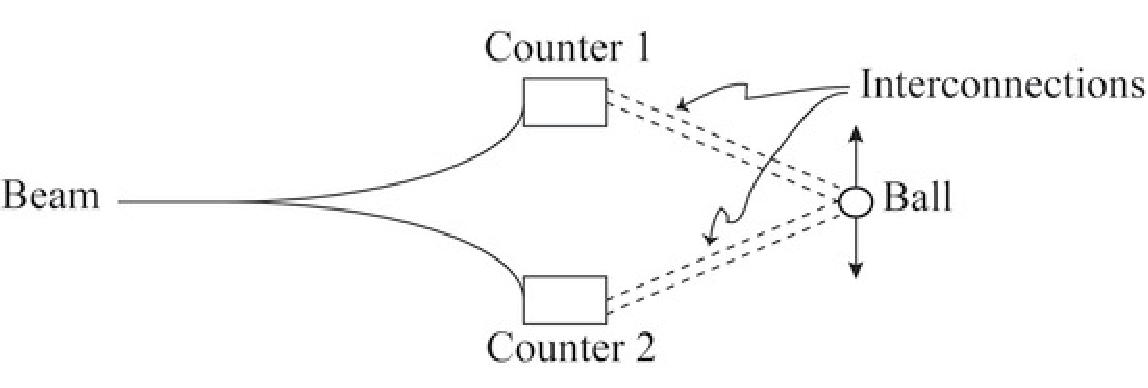
\includegraphics[width=0.8\textwidth]{ART_Kiefer/Kiefer_img.pdf} 
\caption{Feynman's gedanken experiment in which a microscopic
  superposition is transferred to a macroscopic one of a ball being
  simultaneously at two different places. Figure adapted from \cite{de_witt_proceedings:_1957}.}
\end{figure}

In order words, unless one assumes that the superposition principle
and the standard formalism of quantum theory is violated when
gravitational fields play a role (as, for example, Lajos Di\'osi and
Roger Penrose 
envisage), the quantization of gravity seems unavoidable. The majority
of researchers thus accepts the assumption of 
extrapolating the standard linear formalism of quantum theory to
quantum gravity. This holds for almost all of the existing approaches,
from canonical and covariant quantum gravity up to string theory
\parencite{kiefer_quantum_2012}.

At present, there is a discussion about the possibility to observe
gravitational superpositions in the laboratory. There are proposals
to probe a nonclassical gravitational field generated by
two masses each of which is superposed at two locations
\parencite[see e.g.][]{marletto_witness_2017}
or to probe such a field generated by the superposition
of one mass in the spirit of Feynman's proposal cited above
\parencite[see e.g. the remarks in][]{schmole_micromechanical_2016}.
The
observability of such superpositions also meets with criticism 
\parencite{anastopoulos_comment_2018}.

What are the consequences of quantum gravity for our question about the
reality of the wave function? In order to answer this question, it is
sufficient to use the simplest and most conservative approaches to
quantum gravity, which is quantum geometrodynamics.\footnote{Details
  and relevant references can be found, for example, in my monograph
  \parencite{kiefer_quantum_2012}.} One arrives at this theory when asking the
following question: what is the quantum formalism that gives back
Einstein's equations in the semiclassical (WKB) limit? This is analogous
to the heuristic procedure that Erwin Schr\"odinger led to his
equation in 1926.

The canonical formalism of general relativity discloses the real
dynamical quantity of the theory: it is the {\em three-dimensional}
geometry. The configuration space is thus the infinite-dimensional
space of all three-dimensional metrics, with an additional constraint
which guarantees that metrics related by coordinate transformations are
counted only once. The theory possesses four local constraints, which
after Dirac quantization are heuristically transformed into quantum
constraints on physically allowed wave functionals. 
In a shorthand notation, they read
\be
\label {wdw}
\hat{H}\Psi=0,
\ee
where $\hat{H}$ denotes the Hamilton operator of all gravitational and
nongravitational degrees of freedom. The functional $\Psi$ is defined
on the space of three-metrics and nongravitational fields. Equation
\eqref{wdw} is also called Wheeler--DeWitt equation.\footnote{More
  precisely, if written out, \eqref{wdw} includes the Wheeler--DeWitt
  equation and the diffeomorphism constraints.} 

One recognizes from \eqref{wdw} the absence of any external time parameter 
\parencite[see in this context][]{kiefer_does_2015}.
This is obvious for conceptual
reasons. In classical relativity, spacetime (four-geometry) plays the
same role that a particle trajectory plays in mechanics. After
quantization, spacetime has disappeared in the same way as the
particle trajectory has disappeared in quantum mechanics. But whereas
in quantum mechanics Newton's absolute time $t$ has survived, 
no such absolute time is present in Einstein's theory.  
As a result, the fundamental quantum gravity equations are timeless.

Of special concern here is quantum cosmology -- the application of
quantum theory to the Universe as a whole. In the simple case of a
Friedmann universe with scale factor $a$ and a conformally coupled
scalar field $\chi$, the Wheeler--DeWitt equation assumes the form
(after some rescaling and with a suitable choice of units):
\be
\lb{qc}
\hat{H}_0\psi(a,\chi)\equiv (-H_a+H_{\chi})\psi\equiv
\left(\frac{\partial^2}{\partial a^2}-\frac{\partial^2}{\partial\chi^2}
-a^2+\chi^2\right)\psi=0.
\ee

How can one interpret such equations? At the most fundamental level, 
there is no time and there are no classical observers who could
perform measurements. Therefore, the Copenhagen interpretation which
requires the need of classical measurement agencies from the outset,
is inapplicable.  
The question thus arises in which limit
approximate notions of time and observers (more generally, of classical
properties) emerge and what relevance this emergence has for the
interpretation of the wave function. 

Such a limit exists and is well understood \parencite{kiefer_quantum_2012,kiefer_does_2015}. It
is similar to the Born--Oppenheimer approximation in molecular
physics. If one adds inhomogeneous degrees of freedom to the
Hamiltonian in \eqref{qc}, the Wheeler--DeWitt equation is of the form
\be 
\left(H_0+\sum_nH_n(a,\phi,x_n)\right)\Psi(\alpha,
 \phi,\{ x_n\})=0,
\ee
where the $x_n$ stand for the inhomogeneities (gravitational waves,
density perturbations). 
Writing $\Psi=\psi_0\prod_n\psi_n$ and assuming that
$\psi_0$ is of WKB form, that is, $\psi_0\approx C\exp(\I S_0/\hbar)$
(with a slowly varying prefactor $C$), one gets
\be
\I\hbar\frac{\partial\psi_n}{\partial t} \approx H_n\psi_n
\ee
with
\bdm
\frac{\partial}{\partial t}:= \nabla S_0\cdot\nabla.
\edm
This is nothing but a set of time-dependent Schr\"odinger equations
for the inhomogeneities with respect to a time variable $t$ that is
defined from the homogeneous cosmological background;
$t$ is also called `WKB time' and controls the dynamics in this
approximation. Only in this limit can one talk about the probability
interpretation of quantum theory and the existence of observers. It is
thus not at all obvious whether the standard notion of Hilbert space
need, or even can, be extrapolated to the level of full quantum
gravity (beyond this level of the Born--Oppenheimer approximation).

In quantum cosmology, 
 arbitrary superpositions of the gravitational
field and matter states can occur. How can we understand the emergence
of an (approximate) classical Universe? This is achieved by the
process of decoherence introduced above \parencite{kiefer_claus_emergence_2012}. 
Decoherence is a process in
configuration space, and the irrelevant degrees of freedom can be
taken to be part of the inhomogeneities $x_n$. In this way, the scale
factor $a$ and the field $\chi$ can be shown to assume classical
properties. The same then holds for WKB time $t$, which is constructed
from these background variables. 
After this classicality is understood, one can investigate
decoherence for some relevant inhomogeneous degrees of freedom; these
include the inhomogeneities of an inflaton scalar field and
of the metric, giving rise, after decoherence, to the observed CMB
anisotropies and the (not yet discovered) primordial gravitational
waves. In all these considerations, the wave function is assumed to be
real (ontic); this is also the case if one applies collapse models to
quantum cosmology. I should also mention that even the problem of the
arrow of time can, at least in principle, be understood in the
framework of timeless quantum cosmology \parencite{zeh_physical_2007}.

It is clear that the debate about the correct interpretation of
quantum theory will continue, at least until a clear experimental
decision is reached (which could take quite a while). In this
contribution, I have collected arguments which strongly support the
point of view that the wave function is real (ontic), in the same way
as, say, an electric field, is real. Thus, the wave function {\em
  exists}. The perhaps most important open question is: what is the
configuration state for the wave functional at the most fundamental
level? In canonical quantum gravity, it is the space of
three-geometries plus nongravitational fields; what it is at the level
of a fundamental quantum theory of all interactions, is unknown.



%%%%%%%%%%%%%%%%%%%%%%%%%%%%%%%%%%%%%%%%%%%%%%%%%%%%%%%%%%%%%%%%%%

\paragraph{Acknowledgements}

I am grateful to the organizers of the conference
{\em On What Exists in Physics} (Krak\'ow, October~2017) for inviting
me to such an  
inspiring event. I am, in particular, indebted to Professor Micha\l\
Heller for many interesting discussions.

\nocite{einstein_can_1935}
%%%%%%%%%%%%%%%%%%%%%%%%%%%%%%%%%%%%%%%%%%%%%%%




\end{artengenv}

\begin{artengenv}
	{Tadeusz Sierotowicz}
	{Where are Sunspots? The Practical Method of Galileo as an example of Mental Model}
	{Where are Sunspots? The Practical Method of Galileo\ldots}
	{Where are Sunspots? The Practical Method of Galileo as an example of Mental Model}
	{Copernicus Center for Interdisciplinary Studies,\\
		Istituto di Scienze Religiose di Bolzano e IISS Gandhi di Merano}
	{After the publication of \textit{Sidereus Nuncius} Galileo, in the controversy with Ch.
		Scheiner, developed several arguments on behalf of the hypothesis that sunspots are contiguous to the surface of the
		Sun, and presented them in his \textit{Istoria e dimostrazioni intorno alle macchie solari e loro accidenti}
		(Rome 1613).
		%brakuje bibliografii
		One of them, named by Galileo a Practical Method, advocates very clearly the correctness of the
		hypothesis. In the paper the method in question is briefly described. It is argued that the Practical Method is not a
		thought experiment, but rather a mental model proposed precisely in order to solve the problem of sunspots’ location. }
	{sunspots, Galileo’s practical method, mental models, early modern science.}




\section{Introduction}

\lettrine[loversize=0.13,lines=2,lraise=-0.03,nindent=0em,findent=0.2pt]%
{A}{}fter Galileo discovered many celestial novelties through his telescope, as described in the widely read
\textit{Sidereus Nuncius}, his \textit{vis polemica} found a space in the sunspot dispute with the Jesuit priest
Christopher Scheiner (\cite[pp.238–259]{camerota_galileo_2004}; \cite[chap.2.6]{fantoli_galileo:_2003};
\cite{heilbron_galileo_2010,galilei_sunspots_2010-1,shea_galileo_1970,sierotowicz_o_2013})\footnote{Bibliographical note: the
\textit{opera} of Galileo Galilei discussed in the paper can be easily found on the Web: \textit{Istoria e
dimostrazioni\ldots}, \parencite{galilei_istoria_1613} see, e.g., copy of the National Library of Florence: BNCF -
II 461, the Nencini collection: brunelleschi.imss.fi.it/bibliotecagalileo; [\textcolor{black}{Accessed 23 Dec. 2010]}.
In the national edition of the works of Galilei, \textit{Istoria e dimostrazioni\ldots} can be found in the fifth volume:
\parencite[pp.25–239]{favaro_opere_1895}.
Favaro’s edition is cited here with the abbreviation OG, followed
by the number of the volume, the page number, and the verse number. For the English translation, see
\parencite{galilei_sunspots_2010}. Figures: For all details, see
\parencite{sierotowicz_o_2013}.
}. In this article, I pay special attention to a few pages from \textit{Istoria e dimostrazioni intorno alle macchie
solari e loro accidenti}
\parencite{galilei_istoria_1613},
which has been largely neglected by scholars. In the
work, the Pisano\footnote{Galileo is often referred to as the Pisano, after the city of his birth.} presented what he
himself called the most powerful reason in favour of his thesis about the location of sunspots. This is an original
method, called the Practical Method
\parencite[see OG V, 121.5;][p.112]{galilei_sunspots_2010},
through which
Galileo tried to prove his hypothesis by combining in a paradigmatic way sensible experiences (observations) and
necessary demonstrations (a geometrical model).

Galileo Galilei, in opposition to Christopher Scheiner, considered sunspots a phenomenon that exist on the surface of
the Sun and, as a consequence, participate in the rotation of the solar globe. However, according to Scheiner, sunspots
are just shadows of the passage of planets distant from the Sun through the solar disk. All these planets have to move
with an angular velocity that is equal to the angular velocity of the rotation of the Sun.

To decide which of these two theories is right, Galileo proposed several arguments. One of them, a sort of cinematic and
geometric reasoning, was based on the variation of the relative distance between the two spots moving along the same
parallel from the edge of the solar disk towards its centre. The Pisano noted that the observed distance between such
two sunspots changes in a particular way because of the projection on the observation plane of the segment between the
spots according to the angle that the segment forms with the plane of observation. Galileo developed a geometrical
model of this situation in his work on sunspots mentioned above (Fig. \ref{sier-fig1}). 

The apparent distance between two sunspots is normally smaller than the actual distance between them. However, on one
occasion, namely, when the segment between two spots is parallel to the observation plane, the length of the segment
and the length of its orthogonal projection onto the observation plane will be the same. This happens when the straight
line joining the observer’s eye with the centre of the Sun is aligned with the centre of the segment that joins the
spots (Fig. \ref{sier-fig5}). Of course, this situation is rather exceptional, but Galileo was lucky enough to observe it for two
sunspots on 01 July 1613 and 05 July 1613, respectively (Fig. \ref{sier-fig2} and \ref{sier-fig3}). Extraordinary, masterly executed drawings
representing these observations were printed in \textit{Istoria e dimostrazioni\ldots. }In fact, on July 5, 1613, spots A
and B appeared to be symmetrically located with respect to the centre of the solar disk. This particular observation
allowed Galileo to develop and apply the Practical Method. 

\section{The Practical Method}

First, Galileo noted that ``because the distance between the Sun and us is very great in proportion to the diameter of
its body''
\parencite[see OG V, 121.5;][p.112]{galilei_sunspots_2010}
some preliminary premises, also of a physical
nature, for his model can be made: 

\begin{enumerate}
	\item The rays that reach the eye of the terrestrial observer can be considered as parallel lines (see the rays ZDG, OLI,
	and QP in Fig. \ref{sier-fig1});
	\item Sunspots are located on the same latitude and pass through the centre of the solar disk or very close to it; and
	\item This situation occurs in the case of two spots, A and B (see Fig. \ref{sier-fig2} and \ref{sier-fig3}).
\end{enumerate}

Starting with these suppositions, Galileo constructed the geometric model of sunspot observations. The plane of the
drawing (Fig. \ref{sier-fig1}) corresponds to the plane passing through the observer, the centre of the Sun, and the parallel
(practically the equator) on which the sunspots A and B are located. The GDZ line, coming out from the centre of the
Sun G, goes towards the terrestrial observer to whom the spots appear projected on the plane perpendicular to the plane
just mentioned and passing through the centre of the Sun (the observation plane). Let CDE be the semicircle
representing the surface of the Sun, or the parallel on which the A and B spots move, and let the points on the CGE
segment correspond to the observed positions of sunspots in an orthogonal projection on the observation plane. The
points L and H are the sunspots A and B, respectively, observed on 01 July 1613 (Fig. \ref{sier-fig2}). The actual distance between
these spots is equal to the HL chord, but because of the projection effects, these spots are observed as points F and
I, and their observed distance is equal to the length of the FI segment. It is easy to see that in a situation where
the HL segment is symmetrical with respect to the GDZ line, the observed distance should be equal to the length of the
HL segment because the HL, FI, and CGE segments are parallel. This situation actually occurred on 5 July 1613 (see Fig.
\ref{sier-fig3} and \ref{sier-fig5}).

Naturally, the construction described above corresponds to the hypothesis that sunspots are supposed to be located on
the surface of the Sun, or very near to it. What if the spots are but the shadows of a distant planet (Scheiner’s
hypothesis)? Let us now imagine that the phenomenon of the spots is caused by a transition through the solar disk of
objects distant from the surface of the Sun that are about 1/20th of the diameter of the solar disk. The objects in
question therefore move on the MNO semicircle (Fig. \ref{sier-fig1}). In this case, sunspots should be collocated in points N and O,
and their real distance should correspond to the segment NO. It is easy to find out using a compass that the segment NO
is shorter than the HL one. Nevertheless, even in this case, the observed distance corresponds to the FI segment
because the geometric construction represents the way in which the mind and the eye of the terrestrial observer builds
images of the spots. How to decide which of the two situations, clearly different, reflects the real situation? To put
it briefly: where are sunspots -- on the MNO or on the CDE semicircle?

To answer this question, Galileo used a simple and ingenious method, inspired by the observation record of 05 July 1613.
Let the observer execute the drawing that represents this observation and its geometrical reconstruction on the same
scale; that is, let the observer trace the circle that represents the solar disk with the same opening of the compass
for both the geometric reconstruction (Fig. \ref{sier-fig1}) and the recording of the observations (Fig. \ref{sier-fig2} and \ref{sier-fig3}). In these
circumstances, the distance between spots A and B on 05 July directly gives the length of the chord that corresponds to
the real distance between the sunspots in the scale adopted for the drawing. 

Therefore, should the spots be on the surface of the Sun, it would correspond to the HL segment; otherwise, it would
correspond to the NO segment. A graphical manipulation shown on Fig \ref{sier-fig1} and \ref{sier-fig4} clearly indicates that the AB distance
observed on July 1 corresponds to the length of the FI segment. At the same time, reiterating the same operation for
Fig \ref{sier-fig1} and \ref{sier-fig3}, and thus arriving at Fig. \ref{sier-fig5}, it becomes clear that the distance between spots A and B on 5 July 1613 are
equal to the length of the HL segment, which is significantly greater than the length of the NO segment. This confirms
Galileo’s hypothesis.

Galileo must have had this procedure in mind. In fact, in the \textit{Istoria e dimostrazioni\ldots} he wrote, ``now if one
looks at the illustration of the fifth day [Fig. \ref{sier-fig3}], [\ldots] one will find that [the] distance [of the spots] A and B would
be exactly equal to the chord HL. This can in no way happen if their revolution takes place along a circle at any
distance whatsoever from the surface of the Sun''
\parencite[see OG V, 122.34-36;][p.115]{galilei_sunspots_2010}.
Then, he proposed the reasoning summarised above, calculating subsequently the numerical values of the difference
between chords in question (see OG V, 123).
%tu nie ma bibliografii

\section{The Practical Method and its Application}

The Practical Method is a brilliant argument that makes it possible to distinguish between two hypotheses on the
location of sunspots based on observations using a simple and immediate measurement based on a properly scaled
geometric model. The procedure seems to have innovative features. On the one hand, Galileo built a geometric model of
the phenomenon, but on the other hand, the model itself acts as a sort of measuring instrument that allows one to
resolve the dispute between two hypotheses with reference to the observations. It can therefore be said that the
graphical reasoning based on the geometrical model of the event (Fig. \ref{sier-fig5}) permits one to assign a numerical value to a
physical quantity (a distance between sunspots) and solve the problem.

A \textit{sine qua non} condition for such a reasoning to work is to assign the same value to the diameter of the solar
disk both in the construction of the geometric model and for the drawings representing the observations. Galilei
followed precisely this method. In fact, I have analysed a copy of Galileo’s treatise on sunspots from the Early
Printed Books Collection of the Jagiellonian Library in Cracow (593892 II). Here are the results of my measurements
performed on the drawing that corresponds to Fig. \ref{sier-fig1} (accuracy of ± 1 mm.):
\medskip

{\centering
HL = 60mm / ON= 52mm / GM = 69mm / FI = 42mm /\\CE = 123mm / CG = 62mm
\par}
\smallskip

In the same volume, the distance between the sunspots AB is, respectively, 42 mm (observation on 1 July: the diameter of
the solar disk is 123 mm) and 61 mm (observation on 5 July: the diameter of the solar disk is 122 mm).

Therefore, my measurements within the margin of errors seem to indicate that the length of the HL segment is equal to
the distance between the AB spots on 5 July, which in principle solves the ongoing dispute between Galileo and
Scheiner. Of course, things are not that simple because, first, the spots are not exactly point like, and second, they
change shape continuously, moving with their own motion.

In the \textit{Istoria e dimostrazioni\ldots} Galileo applied the Practical Method to other situations, using it as a
starting point for the prediction of the probable results of some possible sunspots observations
\parencite[see OG V, 124.13-21;][p.116]{galilei_sunspots_2010}.
 Suppose, for example, that spot A is collocated
at the edge of the solar disk in point C (Fig. \ref{sier-fig1}), and spot B in point H; then, the arc CGH would be equal to 4°.
Assuming that the GC radius is of 10000 units and the GM radius is of 10100, then the lengths of both the CH, and the
RN segments can be easily calculated; the CH segment would be of 419 units, and the RN of 94 units. The effect would
then be extremely strong (CH/RN = 4.46 versus HL/ON = 1.12 in Fig. \ref{sier-fig5}). Unfortunately, Galileo did not find any
observations corresponding to the situation in question.

\section{The Practical Method -- Methodological Aspects}

How to interpret Galileo’s reasoning? The Practical Method has some characteristics of what is defined in the literature
as an epistemic image. Such visual structures usually serve as a starting point for the formulation and development of
a given theory. The Feynman diagrams are often indicated as an example of this.

Galileo began with some hypotheses that simplified the description of the observational situation (e.g. the parallel
rays that reach the observer) and then constructed a geometric model that, through some mathematical calculations,
permits one to depict the evolution of the phenomenon. The model permits the prediction of the results of the
observations. Galileo’s two-dimensional model becomes, in a sense, a sort of measuring instrument that allows one to
compare directly the two hypotheses by referring them to the observations, solving in this manner a theoretical
problem. 

Thus, it seems reasonable to state that the Practical Method is a reasoning on which is based the argument in favour of
Galileo’s thesis about the location of sunspots. Briefly, the Practical Method is a graphic solution of an analysed
problem. At the beginning of his scientific career, Galileo, in the context of his studies on the centre of gravity of
bodies, emphasised in his discussion with Clavius the importance of drawing in investigation procedures. Lodovico
Cigoli, in a letter to Galileo dated 11 August 1611, wrote that a ``mathematician, even the greatest, without the help
of detailed sketch is only half a mathematician - more, a man without eyes'' (OG XI, 168).

Galileo’s Practical Method thus offers a sort of geometrical reasoning on behalf of his thesis about the location of the
spots. From the mathematical point of view, he constructed a univocal (isomorphic) model of some aspects of the
phenomena that occur on the surface of a sphere. The accuracy of the thesis can be confirmed after having assigned a
numerical value to the crucial physical quantities that assume different values in different scenarios (Galileo’s
\textit{vs} Scheiner’s hypothesis). Here, with great clarity, one can see the connection between geometry and
observations inside a specific model. The Galileo’s Practical Method is therefore an example of model-based reasoning,
which is not the reasoning referred to the figures of syllogism in Aristotelian terms, but -- in this case -- to the
geometric considerations developed inside the model of a specific phenomenon. 

\section{Conclusion -- Galileo’s Practical Method as a Mental Model}

The Practical Method of Galileo assuredly is not an example, or perfect description of what later was called the
Galilean method; the method in which insight into the universe is ``gained through a self-reinforcing loop between
experimental data and theoretical analysis, based on the use of mathematics and modelling''
\parencite[p.2]{succi_big_2019}.
Nevertheless, it contains very valuable hints on how some
natural problems can be solved.

Galileo’s protocol is based on a geometric model, which, starting from simplifying hypotheses, develops an isomorphic
geometric structure of the evolution of a given phenomenon. It allows, as a consequence of some geometrical reasoning,
a direct comparison between the model and the observations, thus providing graphic reasoning on behalf of a specific
thesis as far as a particular aspect of the phenomenon in question (the location of sunspots) is considered. From that
point of view Galileo’s procedure seems to be very similar to what is now called ``mental models'', considered together
with ``mental/thought experiments''\footnote{The bibliography of thought experiments in Galileo is very extensive, e.g.
\parencite{camilleri_knowing_2015,palmerino_discussing_2018,palmieri_mental_2003}.
}, a fundamental evolutionary achievement
of the human race
\parencite[see][]{nersessian_theoreticians_1992,nersessian_creating_2008,stuart_routledge_2018}.

The notion of mental models dates back to the ideas formulated by Charles Peirce and Ludwig Wittgenstein. Kenneth Craik
developed the concept of mental models in a remarkably stimulating way. His theory identified the ability to predict
events as a fundamental property of human thought and as a particularly advantageous adaptive conquest. Regarding
mental models, Craik emphasised their ability to reflect the processes of the real world, both in terms of structure
and in the processes that occur there:
\myquote{
By a model we thus mean any physical or chemical system which
has a similar relation-structure to that of the process it imitates. By ‘relation-structure’ I do not mean some obscure
non-physical entity which attends the model, but the fact that it is a physical working model which works in the same
way as the process it parallels, in the aspects under consideration at any moment
\parencite[p.51]{craik_nature_1943}.}
In short, mental models have a structure similar to the structure of a ``fragment'' of the reality they
represent.

According to Craik, the construction of mental models belongs to the natural capacities of the human mind. The mental
process that constitutes a model is based on three fundamental processes: translation of the processes of the external
world into words, numbers, or symbols; reasoning, that is, the transition to other symbols through deduction,
induction, etc.; and finally, re-translation of these symbols into external processes or the recognition of
correspondence between symbols and external processes.

Since the 1980s, the concept of mental models has been an object of intense research in the fields of philosophy,
literary criticism, computer science, and cognitive science. According to interpretations that follow Craik’s approach,
especially those of Nancy Nersessian, mental models are the constructs of the human mind that represent situations,
events, and processes designed to solve certain problems. These models can be manipulated, transformed, and dynamically
developed through modes of reasoning that are quite different with respect to the forms of reasoning applied to systems
of propositions, such as deduction or induction. In short, there is no strict equivalence between reasoning and logic,
because in the case of mental models, ‘inferences are made through constructing and manipulating models that are
structural, behavioral or functional analog models of target phenomena’
\parencite[p.184]{nersessian_creating_2008}.
Mental experiments are often referred to as an example of this type of ``manipulation'' understood here as a form
of reasoning. Consequently ``\textcolor{black}{thought experimenting is a form of ‘simulative model-based reasoning’''}
\parencite[p.291]{nersessian_theoreticians_1992}.

Galileo’s Practical Method (OG V, 121-122), developed as a measurement tool to be used in the specific dispute on
sunspots, as illustrated above using an example of the drawings from the Jagiellonian Edition, seems to be quite near
to the aforementioned description of mental models. In that sense, his solution to the problem of the location of
sunspots can be considered an example of the construction and the use of mental models. Such models are present in
other discoveries of Galileo, and in the history of physics in the post-Galilean era. However, detailed analysis and
investigation of this topic must be left for future research.


%\section{Illustrations}

\begin{figure}[h]
	\centering
	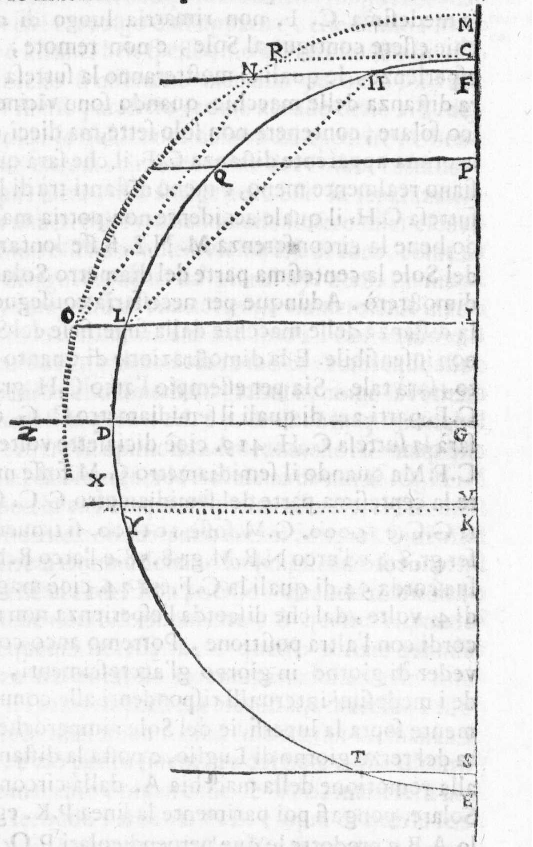
\includegraphics[width=1\textwidth]{ART_Sierotowicz/Sierotowicz_img1-druk.pdf} 
	\caption{Galileo’s Practical Method -- the projection on the observational plane of the segment between two sunspots.}
	\label{sier-fig1}
\end{figure}

\begin{figure}[h]
	\centering
	\includegraphics[width=1\textwidth]{ART_Sierotowicz/Sierotowicz_img2-druk.pdf} 
	\caption{Galileo’s observation on the 1\textsuperscript{st} of July 1613.}
	\label{sier-fig2}
\end{figure}

\begin{figure}[h]
	\centering
	\includegraphics[width=1\textwidth]{ART_Sierotowicz/Sierotowicz_img3-druk.pdf} 
	\caption{Galileo’s observation on the 5\textsuperscript{th} of July 1613.}
	\label{sier-fig3}
\end{figure}

\begin{figure}[h]
	\centering
	\includegraphics[width=1\textwidth]{ART_Sierotowicz/Sierotowicz_img4-druk.pdf} 
	\caption{Sunspots observation, and its geometrical model for the 1\textsuperscript{st} of July 1613. The reconstruction
		by the Author.}
	\label{sier-fig4}
\end{figure}

\begin{figure}[h]
	\centering
	\includegraphics[width=1\textwidth]{ART_Sierotowicz/Sierotowicz_img5-druk.pdf} 
	\caption{Sunspots observation, and its geometrical model for the 5\textsuperscript{th} July. The reconstruction by the
		Author.}
	\label{sier-fig5}
\end{figure}






%\bibitem{camerota_galileo_2004}
%
%\bibitem{camilleri_knowing_2015}
%
%\bibitem{craik_nature_1943}
%
%\bibitem{fantoli_galileo:_2003}
%
%\bibitem{galilei_sunspots_2010}
%
%\bibitem{heilbron_galileo_2010}
%
%\bibitem{nersessian_theoreticians_1992}
%
%\bibitem{nersessian_creating_2008}
%
%\bibitem{palmerino_discussing_2018}
%
%\bibitem{palmieri_mental_2003}
%
%\bibitem{galilei_sunspots_2010-1}
%
%\bibitem{shea_galileo_1970}
%
%\bibitem{sierotowicz_o_2013}
%
%\bibitem{stuart_routledge_2018}
%
%\bibitem{succi_big_2019}
%
%\bibitem{galilei_istoria_1613}
%
%\bibitem{favaro_opere_1895}






\end{artengenv}

\begin{artplenv}{Zbigniew Liana}
	{Nauka jako racjonalna \textit{doxa}. Józefa Życińskiego koncepcja nauki i~filozofii nauki -- poza internalizmem i~eksternalizmem}
	{Nauka jako racjonalna {\pagname{doxa}}\ldots}
	{Nauka jako racjonalna {\tocname{doxa}}. Józefa Życińskiego koncepcja nauki i~filozofii nauki -- poza internalizmem i~eksternalizmem}
	{Uniwersytet Papieski Jana Pawła II w~Krakowie}
	{Science as rational \textit{doxa}. J. Życiński's understanding of science and philosophy of science -- beyond internalism and externalism}
	{Philosophical interests of Joseph Życiński (1948-2011) in the domain of the philosophy of science were focused on the
		debate concerning the nature of science and philosophy of science that followed the Einstein-Planck revolution in
		science. The unexpected discovery of the philosophical, extra-scientific  presuppositions in science, as well as of the
		extra-rational factors determining the way these presuppositions are accepted in science were to be explained within
		the meta-scientific framework. It is the aim of this paper to present Życiński's diagnosis of this post-revolutionary
		situation in the philosophy of science as well as his critique of the metascientific answers to this challenge. The
		reasons will be given why all those answers are put under two dichotomous rubrics of \textit{internalism} and
		\textit{externalism}. It will be also explained how Życiński intends to supersede this false in his opinion opposition
		with a~new concept of doxatic rationality. However the details of the metascientific proposal of Życiński will be given
		only in the subsequent paper. In order to perform the aim of the paper the metatheoretic tools set out by Popper
		\parencite*{popper_beiden_1979}
		%(1979)
		will be used.}
	{rationalism, skepticism, internalism, externalism, scientific revolution, metascientific revolution, philosophical
		presumptions in science, commitment to the research tradition.}


\section*{Wstęp}

\lettrine[loversize=0.13,lines=2,lraise=-0.05,nindent=0em,findent=0.2pt]%
{W}{}przekonaniu Życińskiego dwudziestowieczny spór filozoficzny o~charakter nauki należy interpretować jako kolejny,
historyczny przejaw bardziej fundamentalnego sporu między racjonalizmem a~sceptycyzmem o~racjonalność poznania.

W dwudziestowiecznej tradycji filozoficznej spór o~rozumienie tego, czym jest \textit{nauka}, wiąże się ściśle ze
sporem o \textit{racjonalność} rozwoju wiedzy naukowej. W~swej najbardziej radykalnej wersji -- ,,zewnętrznej'' --
jest to spór racjonalizmu ze sceptycyzmem o~\textit{istnienie}, względnie \textit{nieistnienie} specyficznego, ,,racjonalnego
elementu'' poznania, różnego od zmysłowego postrzeżenia, czyli tak czy inaczej rozumianego \textit{rozumu}. W~swej wersji
,,wewnętrznej'' -- to znaczy wewnątrz tradycji racjonalistycznej, uznającej istnienie \textit{elementu racjonalnego} -- jest
to spór o~charakter tego elementu oraz o~jego miejsce w~procesie zmiany teoretycznej\footnote{Na zasadzie \textit{pars
pro toto} Życiński
\parencite*[s.~184]{zycinski_jezyk_1983}
%\label{ref:RND1yjaBGa3S8}(1983, s.~184)
utożsamia naukę z~,,rozumem naukowym'', a~filozofię nauki
określa na sposób Kanta mianem \textit{Krytyki rozumu naukowego}. Ponieważ w~celu metanaukowej analizy rzeczywistej nauki
tego typu emblematyczne określenie jest mało przydatne ze względu na swą nadmierną ogólność, Życiński wprowadza
bardziej realistyczną kategorię `elementu racjonalnego'
\parencite[s.~142n]{zycinski_jezyk_1983}.
%\label{ref:RNDZsYVuB7lRL}(J. Życiński, 1983, s.~142n).
}.

W diagnozie Życińskiego dwudziestowieczny spór o~\textit{naukę} jest sporem fundamentalnym, sporem o~rozumienie
racjonalności jako takiej, i~to zarówno w~jego wersji ,,zewnętrznej'', jak i~,,wewnętrznej''. W~przypadku sporu
,,zewnętrznego'' -- i~tutaj tkwi \textit{proprium} rozwiązania Życińskiego -- obie strony sporu, czyli rozwiązania zarówno
racjonalistyczne, jak i~sceptyczne, mają wspólny rodowód. Łączy je błędna, tradycyjna koncepcja racjonalności, a~tym
samym błędna koncepcja nauki. W~tezie tej ujawnia się ogólniejsza presupozycja metafilozoficzna postulująca relatywny
charakter sceptycyzmu filozoficznego. Jest to sceptycyzm \textit{względem} określonej koncepcji racjonalności lub
naukowości, a~nie sceptycyzm \textit{w ogóle}. Jest on specyficzną teorią metanaukową odrzucającą \textit{określoną
historycznie} koncepcję naukowości i~racjonalności. W~przypadku sceptycyzmu dwudziestowiecznego, przedmiotu analiz
Życińskiego, negacji podlega koncepcja racjonalności, jaką żywił się dwudziestowieczny racjonalizm metanaukowy,
racjonalizm normatywno-demarkacjonistyczny Koła Wiedeńskiego, Poppera i~Lakatosa\footnote{Zob.
\parencites[s.~228]{zycinski_elementy_1996}[s.~186]{zycinski_jezyk_1983}.
%\label{ref:RNDM0IkZEEMNb}(J. Życiński, 1996, s.~228, 1983, s.~186).
W~tym drugim tekście jest mowa o~porzuceniu ostrej
dychotomii kontekstu odkrycia i~uzasadnienia typowej dla demarkacjonistycznych metodologii.}.

Motywem, który skłonił Życińskiego do postawienia takiej tezy metafilozoficznej, była konstatacja pewnego istotnego
faktu historycznego: to, że oba te przeciwstawne rozwiązania metanaukowe powstały w~reakcji na dwudziestowieczną
rewolucję naukową, która zanegowała dotychczasowy wzorzec naukowości i~racjonalności, wywołując efekt ,,intelektualnego
szoku'' i~prowadząc do ,,rewolucji metanaukowej''. Ale konstatacja faktu z~historii nauki jest jednocześnie interpretacją
sytuacji filozoficznej w~perspektywie metanaukowego sporu o~racjonalność naukową. Jest to zatem ,,konstrukcja''
specyficznego faktu metanaukowego, w~którym już zawiera się \textit{implicite} możliwe rozwiązanie spornego problemu
filozoficznego\footnote{Życiński nie wierzył oczywiście w~istnienie czystych faktów. Zob. niżej przypis \ref{lia-foo-12}. W~tym
wypadku ma swoje zastosowanie teza Lakatosa o~zaślubinach filozofii nauki z~historią nauki
\parencites[zob.][s.~121n]{zycinski_jezyk_1983}[s.~26]{zycinski_structure_1988}[s.~47]{zycinski_struktura_2013}.
%\label{ref:RNDS7T4vadlBl}(zob. J. Życiński, 1983, s.~121n, 1988b, s.~26, 2013, s.~47).
}. Rozwiązanie proponowane przez
Życińskiego jest bezpośrednią konsekwencją przyjętej diagnozy metafilozoficznej: przezwyciężenie problemów związanych z~tradycyjną
koncepcją racjonalności powinno skutkować przezwyciężeniem współczesnego sporu racjonalizmu ze sceptycyzmem.
Konieczna jest zatem istotna modyfikacja tradycyjnego rozumienia racjonalności i~naukowości. Taka, która rozwiąże
problemy nierozwiązywalne na gruncie koncepcji tradycyjnej, a~będące bezpośrednim powodem pojawienia się nowej wersji
sceptycyzmu. W~ujęciu Życińskiego problemy te sprowadzają się do wspólnego mianownika, jakim jest problem pogodzenia
racjonalności naukowej z~występowaniem w~nauce i~w~jej rozwoju \textit{elementów pozanaukowych} i~\textit{czynników
pozaracjonalnych}.

Celem niniejszego artykułu jest analiza wewnętrznej logiki filozofii nauki Życińskiego, jaka prowadzi go od konstatacji
faktów metanaukowych do nowego metateoretycznego rozwiązania kwestii racjonalności naukowej. Panuje dość powszechna
opinia wśród czytelników prac Józefa Życińskiego, że są one trudne w~percepcji ze względu na swą zawiłość,
wielowątkowość, a~przede wszystkim ze względu na specyficzny, retoryczny styl. W~jego tekstach, zwłaszcza pozycjach
książkowych, roi się od przykładów, polemik i~dygresji. Analizy o~wysokim stopniu abstrakcji i~metateoretycznej
precyzji przeplatają się z~argumentami retorycznymi, a~subtelny język analiz miesza się z~literackim językiem ciętej
polemiki. Lekturze jego prac towarzyszy jednak trudna do wyartykułowania intuicja zasadniczej poprawności jego
argumentacji. To właśnie ta intuicja stanowiła dla mnie motywację poszukiwania teoretycznej spójności w~filozofii nauki
Życińskiego.

Metoda poszukiwania wewnętrznej logiki i~ukrytych przedzałożeń jest w~dużej mierze metodą racjonalnej rekonstrukcji.
Wszelkie próby nazbyt deskryptywnego podejścia do filozofii nauki Życińskiego musiałyby ponieść fiasko ze względu na
wspomniany charakter jego prac. Element deskryptywny musi zostać zracjonalizowany za pomocą choćby tymczasowej
metateoretycznej perspektywy interpretacyjnej. Najbardziej zasadne wydaje się wybranie perspektywy wyznaczanej przez
tradycję epistemologiczną, z~jaką Życiński wiąże swoje filozofowanie o~nauce. Pomimo wszystkich jego krytycznych uwag i~zastrzeżeń,
jest to szeroko rozumiana racjonalistyczna tradycja \textit{episteme} (por. \textit{Elementy}, s.~126) w~jej
dwudziestowiecznej wersji zapoczątkowanej przez logiczne badania nad językiem, matematyką i~samą logiką oraz przez
logiczno-metodologiczne badania nad nauką i~jej rozwojem w~ujęciu Poppera i~Lakatosa. Tradycja ta dostarczy
odpowiednich kategorii, przy pomocy których będę mógł rozpocząć analizę tekstów Życińskiego. 

Ogólny, racjonalno-rekonstrukcyjny cel mojego tekstu usprawiedliwia ograniczenie zakresu podejmowanych w~niniejszym
artykule analiz i~wykorzystywanych tekstów źródłowych. Ponieważ nie jest moim celem szczegółowa prezentacja wszystkich
wątków i~wszystkich możliwych niuansów proponowanych przez Życińskiego rozwiązań metanaukowych, dlatego w~artykule
wykorzystane zostaną jedynie jego książki z~zakresu filozofii nauki z~pominięciem licznych, szczegółowych
artykułów\footnote{Są to następujące prace: \textit{Język i~metoda}
\parencite*{zycinski_jezyk_1983},
%\label{ref:RND1LhiGh0y5p}(1983);
\textit{Teizm i~filozofia analityczna}, tom~1
\parencite*{zycinski_teizm_1985},
%\label{ref:RND68nQZEVcjZ}(1985),
\textit{Structure of the Metascientific Revolution}
\parencite*{zycinski_structure_1988},
%\label{ref:RNDgXcIEkiEEw}(1988b),
\textit{Granice racjonalności}
\parencite*{zycinski_granice_1993}
%\label{ref:RND9m82QoDque}(1993)
oraz \textit{Elementy filozofii nauki}
\parencite*{zycinski_elementy_1996}.
%\label{ref:RNDBnf6pOKYn0}(1996).
Wiele wątków powtarza się przez wszystkie prace. Różni je bardziej
sposób prezentacji niż charakter proponowanych rozwiązań. Zauważalna jest zasadnicza ciągłość w~myśli metanaukowej
Życińskiego, począwszy od pierwszej pracy. Tylko w~wybranych przypadkach wskażę pewną ewolucję myśli Życińskiego, inne
pominę, jako nieistotne dla celu mojej pracy. Najbardziej rozwinięte analizy metafilozoficzne Życińskiego można
odnaleźć w~jego \textit{Strukturze rewolucji metanaukowej}
\parencite*{zycinski_structure_1988,zycinski_struktura_2013}.
%\label{ref:RNDPOjzmhEMek}(1988b, 2013).
Tutaj pojawiają się
istotne z~punktu widzenia rozumienia racjonalności nauki koncepcje \textit{ideatów} oraz \textit{ideologicznych programów
badawczych}. Pisząc ten tekst korzystałem z~oryginału angielskiego
\parencite{zycinski_structure_1988}.
%\label{ref:RNDFZPJ2Z2OCH}(J. Życiński, 1988b).
Tekst
ten został przetłumaczony na język polski już po śmierci J. Życińskiego w~2013~r. Cytując fragmenty tej publikacji
korzystam z~przekładu M. Furmana, dokonując wszakże pewnych modyfikacji w~celu dostosowania terminologii do terminologii
niniejszego artykułu. Odnośniki do stron podaję zarówno dla tekstu angielskiego, jak i~dla polskiego przekładu.
Istnieje również drugie, poszerzone wydanie \textit{Elementów} filozofii nauki
\parencite{zycinski_elementy_2015}. \par
%\label{ref:RNDL62LQXHrez}(J. Życiński, 2015). \par
Czytelnikowi, który chciałby poznać najważniejsze myśli całego dorobku Józefa Życińskiego, a~nie tylko z~zakresu
filozofii nauki, polecam przeglądowy artykuł Michała Hellera
\parencite*{heller_filozoficzny_2011}.
%\label{ref:RNDeScsQTkW9D}(2011).
Metanaukowe poglądy Życińskiego omawiam również w~\parencite{evers_can_2016}.
%\label{ref:RNDsr0gJlWoso}(Z. Liana, 2016).
}. Ze względu na obszerność koniecznych analiz zostały one podzielone na dwie odrębne części\footnote{\label{lia-foo-5}Podział ten
dokonany został na prośbę Redakcji.}. Część pierwsza -- zawarta w~niniejszym artykule -- obejmuje sobą najogólniejsze,
metateoretyczne analizy koncepcji Życińskiego filozofii nauki. Część druga zawierać będzie szczegółowe rozwiązania
metanaukowe zaproponowane przez Życińskiego w~celu wypracowania nowego rozumienia nauki i~racjonalności. Są to
rozwiązania najczęściej kojarzone z~jego nazwiskiem, takie jak zasada aracjonalności, zasada epistemologicznej
niepewności, naturalności interdyscyplinarnej, czy też kwestia różnych typów racjonalności i~ewolucji pojęcia
racjonalności.

\section{Perspektywa metateoretyczna}

Nowego rozumienia racjonalności Życiński nie poszukuje na drodze apriorycznych analiz językowo-logicznych, lecz przez
pełniejsze uwzględnienie faktów z~historii nauki. Jego podstawowy postulat metafilozoficzny głosi, że filozofia nauki
powinna zrezygnować z~uproszczonych i~wyidealizowanych koncepcji nauki i~wypracowywać koncepcje bardziej realistyczne,
uwzględniające w~większym stopniu analizę rzeczywistych zachowań naukowców. Tego typu deklaracja metaepistemologiczna
stanowi wyraz określonych przekonań ontologicznych i~metametodologicznych Życińskiego. Element racjonalny ma charakter
\textit{obiektywny}, jest obecny w~nauce realnie, aczkolwiek nierzadko \textit{implicite}. Racjonalność obiektywna ujawnia
swój charakter stopniowo w~meandrach historii nauki. Filozofowi nie pozostaje nic innego, jak uważnie obserwować tę
historię i~próbować \textit{odkrywać }racjonalność obiektywną za pomocą hipotez metanaukowych i~testować te
ostatnie w~oparciu o~faktyczne i~faktualne przejawy racjonalności w~dziejach nauki. Widać z~tego, że pod względem metodologicznym
filozofia nauki Życińskiego bliższa jest nauce empirycznej niż analitycznej. Pod tym względem Życiński staje w~jednej,
\textit{transcendentalnej} tradycji metafilozoficznej obok Poppera i~Lakatosa\footnote{Życiński poddaje jednak tę metodę
reinterpretacji, gdyż inaczej rozumie on \textit{rzeczywistość} nauki niż Popper czy Lakatos. Kwestia ta zostanie
przedstawiona pod koniec artykułu.}.

Swoje koncepcje metafilozoficzne, w~tym koncepcję metody transcendentalnej, Popper przedstawił
najpełniej w~\textit{Die beiden Grundprobleme der Erkenntnistheorie}
\parencite*{popper_beiden_1979}.
%\label{ref:RNDZjoA35m8Sx}(1979).
To właśnie tam broni tezy, że
metodologia jest specyficzną metanauką posługującą się specyficzną metodą transcendentalną\footnote{Koncepcję Poppera
filozofii jako metanauki omawiam szczegółowo w~\parencite{liana_uzasadnienie_2006}.
%\label{ref:RNDfY6Fw7eCi8}(Z. Liana, 2006).
}. Wprawdzie nazwa metody
zaczerpnięta jest od Kanta, to jednak jej rozumienie różni się znacząco od znaczenia, jakie temu wyrażeniu nadawał
Kant. Nie jest to metoda dedukcji transcendentalnej, lecz, jak podkreśla Popper, metoda \textit{analogiczna} do metody
empirycznej. Także w~przypadku metodologii mamy do czynienia z~określonymi faktami filozoficznymi, które wymagają
filozoficznego wyjaśnienia. Wyjaśnienia filozoficzne są wartościowe o~tyle, o~ile wytrzymują konfrontację z~faktami
filozoficznymi. W~pracy tej Popper nie nazywa wyjaśnień metodologicznych hipotezami, a~ich obalenia przez fakty
metodologiczne falsyfikacją. Oba te wyrażenia rezerwuje wyłącznie dla nauk empirycznych. W~metodologii i~w~metodzie
transcedentalnej mamy do czynienia z~tak zwaną \textit{transcedentalną sprzecznością}, analogiczną do empirycznej
falsyfikacji. Metoda ta została zmodyfikowana przez Lakatosa i~poszerzona o~wykorzystanie faktów z~historii nauki w~celu
quasi-empirycznej konfrontacji rozwiązań metanaukowych. Życiński przyjmuje w~filozofii identyczną transcendentalną
metodę, z~tym że terminy `falsyfikacja' i~`hipoteza' odnosi on bez żadnego rozróżnienia zarówno do metody nauk
empirycznych, jak i~do metody metanauki lub szerzej filozofii nauki\footnote{W jego tekstach można znaleźć wiele
wypowiedzi o~\textit{falsyfikacji }koncepcji filozoficznych
\parencites[s.~177]{zycinski_teizm_1985}[s.~9,12,97,135]{zycinski_structure_1988}[s.~17,22,174,239]{zycinski_struktura_2013}.
%\label{ref:RNDlMUuFKby8S}(J. Życiński, 1985, s.~177, 1988b, s.~9,12,97,135, 2013, s.~17,22,174,239).
W~\textit{Elementach}
\parencite*[s.~166]{zycinski_elementy_1996}
%\label{ref:RNDCkkQxwcbWF}(1996, s.~166),
mówi o~wymogu
\textit{falsyfikowalności} rozwiązań metanaukowych. Życiński odróżnia falsyfikowalne hipotezy metanaukowe od
niefalsyfikowalnych idei metafizycznych. Za Popperem uznaje metafizykę za \textit{zasadniczo niefalsyfikowalną}
\parencite[s.~130]{zycinski_elementy_1996}.
%\label{ref:RNDA2elxmxDEm}(J. Życiński, 1996, s.~130).
}.

Należy też zauważyć, że Życiński rozróżnia wąsko rozumianą metanaukę od szerszej filozofii nauki
\parencite[s.~14–16]{zycinski_elementy_1996}.
%\label{ref:RNDSXNKAbqry1}(J. Życiński, 1996, s.~14–16).
Metanauka bada kwestie logiczne,
metodologiczne i~epistemologiczne w~nauce. Filozofia nauki zajmuje się z~kolei wypracowaniem całościowej wizji nauki w~jej ujęciu
diachronicznym, czyli strukturą rewolucji naukowych, związkami między czynnikami racjonalnymi i~socjologicznymi,
ewolucją pojęcia racjonalności. Nie należy ich wszakże sobie przeciwstawiać, gdyż obie zajmują się ,,tą samą
rzeczywistością nauki'' a~granice między nimi są do pewnego stopnia \textit{rozmyte}
\parencite[s.~16]{zycinski_elementy_1996}.
%\label{ref:RNDJqZXflfCwo}(J. Życiński, 1996, s.~16).
Metoda transcedentalnej falsyfikacji stosuje się do nich obu.

Z perspektywy analizy koncepcji Życińskiego szczególnie przydatne wydaje się wprowadzone przez Poppera pojęcie
\textit{faktu metodologicznego} lub \textit{epistemologicznego}, czyli \textit{faktu metanaukowego}\footnote{Dla ułatwienia
lektury w~całym tekście treść idei, podobnie jak treść pojęć i~koncepcji, piszę zazwyczaj kursywą. Kursywa służy
również do podkreślenia istotnych elementów znaczeniowych.}. W~kontekście filozofii Życińskiego można pojęcie to
rozszerzyć do pojęcia \textit{faktu filozoficznego}. Pojęcia te, jakkolwiek budzą w~niektórych kręgach filozoficznych
sprzeciw i~opór, to jednak w~perspektywie współczesnej filozofii nauki odrzucającej ,,zgodnie'' -- podobnie jak Popper --
istnienie \textit{czystych faktów}, są one jak najbardziej na miejscu. Skoro fakt rozumiany jako pewne zdanie bazowe
nauki lub metanauki jest w~sposób nieunikniony teoretyczną interpretacją obserwacji\footnote{\label{lia-foo-12}O ile w~czasach Poppera i~Koła
Wiedeńskiego teza ta była przedmiotem sporu, o~tyle w~czasach Życińskiego była ona już podstawowym i~,,niekontrowersyjnym''
założeniem filozofii nauki. Życiński uznaje ten fakt to za skutek rewolucji metanaukowej
\parencite[zob.][s.~127]{zycinski_elementy_1996}.
%\label{ref:RNDNNdGM9DYkK}(zob. J. Życiński, 1996, s.~127).
}, to staje się on pojęciem analogicznym. W~zależności od
typu interpretacji mamy do czynienia z~faktem empirycznym, filozoficznym, naukowym lub metanaukowym,
etc. W~,,socjologicznej'' koncepcji faktu wprowadzonej przez Poppera\footnote{Termin `socjologiczna' oznacza według Poppera
konieczność intersubiektywnej zgody. Warto zauważyć, że według niego chodzi o~zgodę ,,negatywną'', a~nie pozytywną. Ta
ostatnia implikowałaby swoisty indukcjonizm, który, jak wiadomo, jest dla Poppera niemożliwy do zaakceptowania z~racji
logicznych. Zgodę faktualną uznaje się za obowiązującą wtedy, gdy nikt \textit{kompetentny} (\textit{sic!}) nie wyraża
sprzeciwu, i~to tylko tymczasowo, do chwili, gdy pojawi się ktoś \textit{kompetentny} zgłaszający sprzeciw. Taki sprzeciw
zmusza do rewizji zdań faktualnych. Najpełniejsze przedstawienie ,,negatywnej'' koncepcji \textit{faktu} można odnaleźć w~pracy Poppera
\parencite*[s.~122–135, zwł. 131n.]{popper_beiden_1979}
%\label{ref:RNDFSE3yxffmO}(1979, s.~122–135, zwł. 131n.).
} stopień obiektywności faktu mierzy się stopniem
jego intersubiektywności. Z~tego względu fakty filozoficzne cechują się znacznie mniejszym stopniem obiektywności niż
fakty empiryczne i~w~konsekwencji możliwość obalenia koncepcji metanaukowych przez fakty filozoficzne jest dużo
mniejsza niż możliwość falsyfikacji hipotez empirycznych. O~ile Popper już w~\textit{Die beiden Grundprobleme} zaczął
wątpić w~możliwość rozstrzygającego obalenia na gruncie metodologii, o~tyle u~Życińskiego niełatwo znaleźć artykulacje
podobnych wątpliwości\footnote{Mówi on o~falsyfikacji \textit{tout court} metanaukowej koncepcji teorii nauki
obiektywnej
\parencites[s.~9]{zycinski_structure_1988}[s.~17]{zycinski_struktura_2013},
%\label{ref:RNDwQZn2Zd98X}(J. Życiński, 1988b, s.~9, 2013, s.~17),
albo o~\textit{praktycznej} falsyfikacji
intuicjonizmu w~matematyce
\parencites[s.~97]{zycinski_structure_1988}[s.~174]{zycinski_struktura_2013}.
%\label{ref:RNDF7UBvcuK26}(J. Życiński, 1988b, s.~97, 2013, s.~174).
Jednocześnie jednak Życiński
\parencites*[s.~140]{zycinski_structure_1988}[s.~248]{zycinski_struktura_2013}
%\label{ref:RNDhVrobTs8jG}(1988b, s.~140, 2013, s.~248)
krytykuje Poppera i~jego tezę o~możliwości obiektywnej
oceny wartości schematów pojęciowo-metodologicznych. W~świetle \textit{Die beiden Grundprobleme} nie wydaje się, by teza
ta faktycznie była głoszona przez Poppera, a~po drugie, jej krytyka wydaje się niezbyt spójna z~niekrytycznym użyciem
przez Życińskiego terminu `falsyfikacja'.}.

\section{Rewolucja naukowa a~rewolucja metanaukowa -- narzędzia metateoretycznej analizy}

Punktem wyjścia dla Życińskiego do poszukiwania nowych rozwiązań metanaukowych i~z~zakresu filozofii nauki jest swoista
metahistoryczna i~metanaukowa teza. W~filozofii nauki doszło do \textit{metanaukowej rewolucji}, która została wywołana
przez wcześniejszą rewolucję naukową\footnote{Termin `rewolucja metanaukowa' pojawia się już
w~\parencite[s.~99]{zycinski_jezyk_1983}
%\textit{Języku i~metodzie} \label{ref:RNDX1VVM27OlW}(J. Życiński, 1983, s.~99)
w~tytule drugiej części dzieła: ,,Struktura rewolucji
metanaukowych''. Ten sam tytuł nosi angielska książka Życińskiego
\parencite*{zycinski_structure_1988},
%\label{ref:RNDZhnNjGxqOR}(1988b)
będąca rozwinięciem
idei zawartych w~\textit{Języku i~metodzie}. Życiński mówi o~odstępie ,,półwiecza'' między rewolucją naukową a~rewolucją
metanaukową. Wyrażenie pojawia się
w~\parencite[s.~101]{zycinski_jezyk_1983}
%\textit{Języku i~metodzie} \label{ref:RNDIDOT0gvEdV}(J. Życiński, 1983, s.~101)
i~zostaje powtórzone w~\parencite[s.~126]{zycinski_elementy_1996}.
%\textit{Elementach...} \label{ref:RNDTq4UOwaMNQ}(J. Życiński, 1996, s.~126).
}.
Jedna i~druga były
równie gwałtowne, powiązane z~doświadczeniem rzeczonego intelektualnego szoku. W~celu rekonstrukcji logiki ukrytej w~rozwiązaniu
Życińskiego konieczne wydaje się poddanie analizie specyficznej relacji, jaka zachodzi w~jego koncepcji
między dwoma faktami: między faktem rewolucji naukowej a~faktem rewolucji metanaukowej.

Język, jakim Życiński operuje w~kontekście omawiania relacji między rewolucją metanaukową a~rewolucją naukową, jest
zarówno językiem logiki, jak i~językiem psychologii. Jest językiem logiki, gdyż mówi o~\textit{implikowaniu} rewolucji
metanaukowej przez rewolucję naukową oraz o~metanaukowych \textit{konsekwencjach} rewolucji naukowej
%\label{ref:RND7WtbaMWBYd}(J. Życiński, 1988b, s.~8.13, 2013, s.~15.24)
\parencites[s.~8.13]{zycinski_structure_1988}[s.~15.24]{zycinski_struktura_2013}\footnote{Polski przekład `rezultat' nie oddaje
wiernie angielskiego `implied'.}. Język ten sugeruje, iż Życiński postuluje istnienie silnych związków
merytoryczno-\mbox{-logicznych} %notabene
pomiędzy tymi rewolucjami. Teoretyczne rozwiązania zaproponowane w~ramach rewolucji
metanaukowej nie miały zatem genezy czysto apriorycznej, lecz były w~dużej mierze  zdeterminowane rzeczywistą nauką.
Ale z~drugiej strony Życiński mówi o~\textit{szoku} wywołanym przez rewolucję naukową wśród filozofów nauki i~o~ich
reakcji na ten szok. Także sam termin `rewolucja' użyty przez Życińskiego niesie ze sobą silne konotacje pozalogiczne.
Został wprowadzony do filozofii nauki przez Kuhna w~celu podkreślenia istotnej roli czynników socjologicznych,
psychologicznych i~kulturowych w~rozwoju nauki. Odrzucając dychotomię skrajnego internalizmu i~skrajnego eksternalizmu,
Życiński odrzuca zarówno koncepcję relacji czysto logicznej, jak i~koncepcję relacji czysto ,,zewnętrznej'',
przyczynowej. W~konsekwencji przedstawia tę relację dwoiście, zarówno jako związek logiczny, racjonalny, jak i~jako związek
przyczynowo-\mbox{-skutkowy}\footnote{Nie %notabene
jest możliwe przedstawienie koncepcji Życińskiego w~sposób liniowy, niejako ,,cegiełka
po cegiełce''. Ponieważ to, w~jaki sposób dokonuje on metanaukowej interpretacji faktów historycznych i~relacji między
nimi, jest już warunkowane \textit{implicite} przez jego metanaukowe koncepcje, dlatego nieunikniona jest pewna kolistość
prezentacji i~przyjęcie na początku pojęć, które będą wyjaśniane dopiero z~czasem. Pojęcia \textit{internalizmu} i~\textit{eksternalizmu}
zostaną przedstawione w~punkcie \ref{lia-sec-5}, a~psychologiczne pojęcie \textit{szoku} w~punkcie \ref{lia-sec-4}b.}.

Życiński podejmuje studium i~analizę historii nauki i~historii filozofii nauki w~celu zidentyfikowania różnego typu
faktów metanaukowych, zarówno racjonalnych, jak i~pozaracjonalnych, które pozwolą mu na właściwą interpretację zależności
rewolucji metanaukowej od rewolucji naukowej. Z~jednej strony poszukuje faktów pozaempirycznych metanaukowych z~historii
nauki, które pozwolą mu na uchwycenie racjonalnych (logiczno-merytorycznych) relacji zachodzących pomiędzy
zmianami na poziomie nauki teoretycznej a zmianami na poziomie teorii metanaukowych (zmian metateoretycznych). Z~drugiej
strony poszukuje faktów ,,psychologicznych'' usprawiedliwiających (potwierdzających) użycie psychologicznych
kategorii `rewolucji' i~`intelektualnego szoku'\footnote{Ponieważ pojęcie \textit{kategorii} traktuję jako pojęcie
metateoretyczne i~metajęzykowe zarazem, dlatego treść kategorii będę zapisywał w~cudzysłowie metajęzykowym.} dla opisu
stanu umysłu filozofów nauki.

Poniżej przedstawiam w~formie metateoretycznych uwag wyjaśnienie różnych typów faktu metanaukowego. Uwagi te są
przydatne do lepszego zrozumienia dalszych analiz, ale nie są konieczne. Jako bardziej abstrakcyjne i~niekonieczne do
dalszej lektury zostały wydzielone z~całości tekstu.\footnote{W całym artykule bardziej abstrakcyjne analizy
metateoretyczne lub metafilozoficzne przedstawiam w~formie oddzielnych uwag. Mam nadzieję, że ułatwi to lekturę
tekstu. W~obecnym artykule nie podejmuję szczegółowej analizy metody, jaką Życiński posługuje się w~filozofii nauki. Byłaby to
niewątpliwie niezwykle interesująca strategia poszukiwania ukrytych presupozycji Życińskiego na temat racjonalności
metodologicznej, ale zaciemniłoby to dodatkowo i~tak stosunkowo skomplikowany tekst artykułu. Dlatego ograniczam się w~tym
względzie do rzeczonych uwag.}

\begin{uwaga}
Fakty metanaukowe to quasi-empiryczne fakty z~historii nauki. będące przedmiotem wyjaśnień
metanaukowych. Idea wyróżnienia faktów empirycznych od quasi-empirycznych faktów metanaukowych pochodzi od Poppera.
Wprawdzie Życiński nie stosuje tego typu terminologii, niemniej mówi o~faktach z~historii nauki będących przedmiotem
wyjaśnień metanaukowych. Odróżnienie Poppera ma charakter demarkacjonistyczny. Na gruncie metodologicznym odróżnia on
wyraźnie fakty (zdania) empiryczne od faktów epistemologicznych, czy metodologicznych. Jego teoria
\textit{metodologicznych typów} faktów bazuje na specyficznej \textit{zasadzie analogii}: fakty epistemologiczne są
analogiczne do faktów empirycznych, podobnie jak metoda filozofii nauki (metoda transcedentalna) jest analogiczna do
metody empirycznej. W~przypadku Życińskiego, jego teksty sugerują, że operuje on raczej jednoznacznym niż analogicznym
pojęciem faktu we wszystkich kontekstach metodologicznych. Brak wystarczających danych, by rozstrzygnąć, czy jest to
świadoma i~krytyczna postawa metodologiczna, czy jedynie spontaniczna. Z~tego względu zastosowaniu terminologii Poppera
do interpretacji tekstu Życińskiego musi towarzyszyć daleko posunięta ostrożność hermeneutyczna. Tego typu ostrożna
interpretacja terminu `fakt metanaukowy' abstrahuje od meta-metodologicznych idei Poppera i~ogranicza znaczenie tego
terminu do własności \textit{bycia faktem wyjaśnianym przez metanaukę}.
\end{uwaga}

\begin{uwaga}
Fakt metanaukowy, analogicznie do faktu empirycznego, stanowi językowe przedstawienie i~zarazem
teoretyczną interpretację konkretnego, postrzeganego zmysłami ,,zdarzenia''. W~nie-demarkacjonistycznym ujęciu
Życińskiego zdarzeniem ujmowanym przez fakt metanaukowy może być zarówno zjawisko fizyczne (np. psychologiczne), jak i~zjawisko
,,językowe''. Takim zjawiskiem językowym jest pojawienie się określonego twierdzenia lub teorii o~określonych
cechach ontologicznych lub logicznych. Może nim być także zachowanie metajęzykowe i~zarazem metanaukowe
(epistemologiczne, metodologiczne) naukowca: to, co robi on ze swoimi wypowiedziami, by je uzasadnić, obalić,
sprawdzić, a~także to, do jakich celów poznawczych ich używa.

Ze względu na dwa typy faktów metanaukowych: empiryczne fakty metanaukowe i~pozaempiryczne ,,językowe'' fakty metanaukowe,
te ostatnie będę nazywał `faktami metateoretycznymi'.

W perspektywie metajęzykowej fakt metateoretyczny należy utożsamić ze zdaniem egzystencjalnym orzekającym występowanie
\textit{typowych} (powtarzających się) cech metateoretycznych (np.: ,,Naukowcy dokonują predykcji'', ,,Fakty naukowe są
obciążone teoretycznie'', ,,Nauka nie potwierdza ostrego odróżnienia kontekstu odkrycia od kontekstu uzasadnienia'',
,,Teorie się zmieniają'', ,,Mechanika kwantowa odchodzi od tradycyjnego ideału poznania jednoznacznego'', ,,Twierdzenia
limitacyjne metalogiki ukazują granice poznania matematycznego i~logicznego'' itp.), a~konkretne zdarzenia z~historii
nauki z~desygnatami spełniającymi lub nie to zdanie. 

Stwierdzenie powyższe pokazuje, że wyrażenia `wyrażenie metateoretyczne' i~`wyrażenie metajęzykowe' nie są tożsame.
Fakty metateoretyczne można (i należy) traktować jako język przedmiotowy metanauki. Metanauka ma swój własny język
przedmiotowy i~swój własny metajęzyk, różny od języka i~metajęzyka nauk przedmiotowych. Osobnym problemem jest pytanie,
czy język przedmiotowy metanauki jest metajęzykiem nauki przedmiotowej i, w~konsekwencji, czy metajęzyk metanauki jest
meta-metajęzykiem nauki przedmiotowej. Szczegółowa odpowiedź na tak postawione pytanie wykracza poza ramy niniejszego
artykułu. Ale w~metodologistycznym podejściu Poppera do metanauki zdania metanauki mają za przedmiot wyrażenia
metajęzykowe nauki przedmiotowej tylko w~ich ujęciu `materialnym', a~nie `formalnym'. Metanauka tworzy własny język
przedmiotowy na bazie metajęzyka nauki przedmiotowej. Ten język przedmiotowy nie utożsamia się z~metajęzykiem nauk
przedmiotowych, a~jedynie powstaje na drodze odpowiedniej interpretacji metodologicznej metajęzykowych (i zarazem
metanaukowych) zachowań naukowców (względem faktów, teorii etc.) jako zachowań metateoretycznych lub innych (np.
psychologicznych). Nie należy również mylić metanauki jako dyscypliny filozoficznej z~metanaukowymi \textit{zachowaniami}
naukowców. Te ostanie to te zachowania naukowców, które są przedmiotem metanaukowej interpretacji w~filozofii nauki.

Warto przy tym zauważyć, że samo odróżnienie dwóch dziedzin faktów metanaukowych: dziedziny metateoretycznej (historia
nauki rozumianej intersubiektywistycznie) i~dziedziny empirycznej (świat, w~tym także subiektywne reakcje i~uwarunkowania
naukowców) jest już wyrazem określonej interpretacji metanaukowej (albo jeszcze wyższego rzędu
metanaukowego) określonych intuicji poznawczych.
\end{uwaga}

\begin{uwaga}
Faktów metateoretycznych nie należy utożsamiać z~\textit{konkretnymi} przypadkami z~historii nauki.
Fakty te są przedstawieniem ogólnie ujętych, określonych cech -- ontologicznych lub metateoretycznych -- teorii naukowych
i zachowań epistemologiczno-metodologicznych naukowców. Konkretne przypadki z~historii nauki stanowią co najwyżej
\textit{ilustrację}, \textit{przykład} lub \textit{potwierdzenie} występowania tego typu cech w~nauce. Swego czasu August
Comte rozróżnił \textit{fakty jednostkowe} od \textit{faktów ogólnych}. Naukę empiryczną i~filozofię o~wiele bardziej
interesują fakty ogólne -- czyli to, co jest powtarzalne -- niż konkretne jednostkowe przypadki (zdarzenia). Nawet
w~procedurze potwierdzenia lub obalenia empirycznego pojedyncze zdarzenia są bezwartościowe metodologicznie. Muszą być
powtarzalne i~muszą się pewną ilość razy powtórzyć -- najlepiej niezależnie -- by mogły zostać \textit{zaakceptowane} w~sposób
intersubiektywny przez wspólnotę badaczy. Jak wiadomo, Popper nazywa te \textit{fakty ogólne} zdaniami bazowymi i~hipotezami
niskiego rzędu.

Z tego względu fakt metateoretyczny -- fakt pozaempiryczny, czyli fakt w~perspektywie metody innej niż metoda empiryczna
-- to sąd egzystencjalny, który dotyczy nauki (względnie metanauki) rozumianej zarówno w~jej aspekcie funkcjonalnym,
jak i~przedmiotowym. W~pierwszym przypadku fakt metateoretyczny dotyczy zachowań metodologicznych naukowców (względnie
filozofów nauki), w~drugim wystąpienia określonych sądów, twierdzeń, teorii, hipotez, idei, a~także ich własności
metateoretycznych (względnie meta-metateoretycznych).
\end{uwaga}

\begin{uwaga}
Osobną kwestią jest problem zaklasyfikowania faktów psychologicznych odnotowujących reakcje
psychologiczne w~obliczu nowej nauki. W~demarkacjonistycznym ujęciu Poppera należy je uznać za fakty \textit{stricte}
empiryczne nienależące do metanauki. W~przypadku nie-demarkacjonistycznego ujęcia Życińskiego -- gdzie element
\textit{stricte} racjonalny współwystępuje z, i~jest dookreślany przez element przyczynowy -- należy przypuszczać, że
podział nie jest tak ostry i~także fakty psychologiczne z~historii nauki są specyficznymi faktami metanaukowymi.

Inna sprawa, że w~historii nauki te dwa typy ,,faktów'' nie występują ,,oddzielnie'', lecz tworzą \textit{jeden}
\textit{złożony} fakt metanaukowy: bezpośredni przedmiot obserwacji. Fakt złożony (to znaczy fakt ,,surowy'' --
uteoretyzowany w~mniejszym stopniu) można ,,rozłożyć'' -- to znaczy zinterpretować i~wyjaśnić dedukcyjnie -- na wspomniane
dwa \textit{typy} lub\textit{ aspekty} metanaukowe (na fakt empiryczny i~na fakt \textit{stricte} metateoretyczny, to znaczy
pozaempiryczny) dopiero za pomocą odpowiedniej analizy metanaukowej.

Niezależnie od \textit{faktycznej} struktury faktów metanaukowych i~niezależnie od \textit{faktycznego} charakteru
metanaukowych faktów psychologicznych, rozróżnienie empirycznych i~pozaempirycznych (metateoretycznych) faktów
metanaukowych jest pragmatycznie użyteczne. Nie należy traktować tego rozróżnienia skrajnie demarkacjonistycznie, jak
chciał Popper, lecz wyłącznie jako pierwsze przybliżenie metanaukowe tego, czym jest fakt metanaukowy. Jego użyciu, w~perspektywie
metafilozofii Życińskiego, musi towarzyszyć zawsze odpowiednie ograniczenie, że wszelkie demarkacje mają
charakter wyłącznie idealizacyjny i~nigdy nie stanowią ostatecznego ujęcia rzeczywistości racjonalnej.
\end{uwaga}

\begin{uwaga}
Życiński nie przeprowadza tego typu analiz metateoretycznych w~odniesieniu do stosowanej przez siebie
terminologii metanaukowej. W~konsekwencji nie rozróżnia on \textit{explicite} pod względem metodologicznym ani faktu
naukowego od metanaukowego, ani tym bardziej obu aspektów tego ostatniego. Konkretne znaczenie metateoretyczne,
jakie wiąże z~terminem `fakt', określane jest przez kontekst użycia.
\end{uwaga}
	
Przyjmując wraz Życińskim, że w~rekonstrukcji historii nauki i~historii filozofii nauki związki logiczne są ważniejsze
od uwarunkowań psycho-społecznych, w racjonalnej rekonstrukcji jego rozumienia relacji między rewolucją naukową a~rewolucją
metanaukową należy przyjąć, że najważniejsze są w~tym wypadku związki pomiędzy specyficznymi faktami
metateoretycznymi z~dziedziny nauki przedmiotowej (np. teoriami, założeniami) a~specyficznymi faktami metateoretycznymi z~dziedziny
metanauki (np. wyjaśnieniami)\footnote{W perspektywie przyjętych rozróżnień między poziomami naukowości i~teoretyczności
należałoby nazwać te ostatnie fakty \textit{faktami meta-metateoretycznymi}. Ale takie rozróżnianie nic
nie wniesie do dalszych analiz poza zbędnym balastem precyzji. Życiński wydaje się nie przywiązywać dużej wagi do tego
typu precyzyjnych rozróżnień poziomów analiz.
W~\parencite[s.~123]{zycinski_jezyk_1983}
%\textit{Języku i~metodzie} \label{ref:RNDqQTlKikSxt}(J. Życiński, 1983, s.~123)
przytacza sceptyczną uwagę J. Watkinsa odnośnie do tego typu rozróżnień u~Poppera i~Lakatosa, ale nie wydaje na
ten temat własnej oceny.}. Metanaukowych faktów psychologicznych w~takiej rekonstrukcji nie można pominąć, jeśli nie
chcemy przypisać Życińskiemu koncepcji nazbyt uproszczonej i~wyidealizowanej, ale też nie mogą być one, jak zobaczymy
poniżej, dominujące\footnote{Uzasadnienie tych warunków zostanie przedstawione niżej przy okazji omawiania własnego
rozwiązania metanaukowego Życińskiego.}.

Wedle takiej rekonstrukcji Życiński najpierw ustala odpowiednie zbiory faktów metateoretycznych obu typów, a~następnie
poszukuje właściwych relacji merytoryczno-logicznych pomiędzy nimi. Wyznaczenie odpowiednich zbiorów faktów
metateoretycznych jest stosunkowo proste. Czerpie je odpowiednio z~historii nauki przedmiotowej
(empirycznej i~formalnej) z~jednej strony i~z~historii metanauki z~drugiej. Problematyczny jest natomiast sposób poszukiwania
powiązanych merytoryczno-logicznie \textit{uporządkowanych par} faktów metateoretycznych: 

\smallskip
{\centering
	{\textless}fakt z~historii nauki; fakt z~historii metanauki{\textgreater}.
\par}
\smallskip


W tym celu Życiński wydaje się odwoływać do idei powiązania faktów psychologicznych z~faktami metateoretycznymi w~postaci
surowych faktów metanaukowych i~meta-metanaukowych\footnote{Fakty meta-metanaukowe to fakty tworzące
rzeczywistość metanauki jako pewnej działalności poznawczej człowieka.}. Idea ta kieruje \textit{implicite} jego
heurystyczną strategią metanaukową: psychologiczna idea \textit{intelektualnego szoku} i~kategorii jemu równoważnych
nadaje się na stosunkowo łatwe kryterium wyróżniania tych faktów metateoretycznych z~dziejów nauki, które doprowadziły
do zmian w~metanauce, czyli do nowych faktów metateoretycznych w~dziejach metanauki. Ponieważ psychologiczny aspekt
faktów metanaukowych jest łatwiejszy do konstatacji, zatem może służyć jako wygodne narzędzie wyróżniania odpowiednich
pozaempirycznych faktów metateoretycznych obu typów i~ich związków. Z~jednej strony należy poszukiwać takich teorii
naukowych i~takich cech tych teorii, które wywołały szok wśród filozofów nauki, a~z~drugiej strony takich postaw
metanaukowych i~teorii metanaukowych, które były odpowiedzią na ów szok. Oczywiście, zgodnie z~zasadniczo
racjonalistycznym stanowiskiem Życińskiego, warunkowanie psychologicznie w~żadnym wypadku nie może wyjaśniać ani
zastępować związków logicznych, jakie występują między obu typami faktów metateoretycznych. W~tym celu konieczna jest
klasyczna analiza znaczeń i~struktur logicznych.

Oprócz \textit{szoku intelektualnego} Życiński wskazuje także na inne psychologiczne fakty metanaukowe w~kontekście
powiązania rewolucji naukowej z~metanaukową. Jednym z~nich jest odczucie \textit{paradoksalności} nowych teorii. W~\textit{Strukturze
rewolucji metanaukowej} pisze, że szok intelektualny towarzyszył zarówno odkryciu
\textit{paradoksalnych} geometrii nieeuklidesowych, antynomii w~podstawach matematyki, jak i~\textit{paradoksów} teorii
kwantów oraz teorii względności. W~okresie rewolucji naukowej doświadczenie paradoksalności nauki było do tego stopnia
powszechne, że niektórzy, jak na przykład Niels Bohr, uznali ją za synonim poprawności i~prawdziwości rozwiązań
teoretycznych\footnote{Zob.
\parencites[s.~9,132]{zycinski_structure_1988}[s.~16,233]{zycinski_struktura_2013},
%\label{ref:RNDsmv0TXVWdS}(J. Życiński, 1988b, s.~9,132, 2013, s.~16,233),
gdzie mówi o~wymogu
stawianym teorii naukowej przez Bohra, by była ,,dostatecznie szalona''.}. Podobną reakcją psychologiczną było
\textit{zaskoczenie} spowodowane odkryciem nieoczekiwanych cech nauki, takich jak istnienie wewnętrznych, niepokonalnych,
logicznych ograniczeń. I~to zarówno w~obrębie nauk przedmiotowych (formalnych i~empirycznych), jak i~w~obrębie
metanauki: odkrycie niezupełności bogatych systemów logicznych, zasady losowości w~fizyce czarnych dziur czy zasady
nieoznaczoności Heisenberga oraz odkrycie metanaukowej zasady niedookreślenia teorii przez obserwacje
\parencites[s.~11]{zycinski_structure_1988}[s.~20]{zycinski_struktura_2013}.
%\label{ref:RND6Rd4uQGI6n}(J. Życiński, 1988b, s.~11, 2013, s.~20).

Wewnętrzna logika kierująca przejściem od rewolucji naukowej do rewolucji metanaukowej wydaje się być zatem w~rozumieniu
Życińskiego następująca. Pojawienie się nowej teorii naukowej o~określonych cechach (fakt metateoretyczny) wywołuje
szok intelektualny (fakt psychologiczny), a~ten z~kolei \textit{przyczynowo} prowadzi do zaproponowania nowych koncepcji
metanaukowych (fakt metateoretyczny wyższego rzędu), przy czym treść tych ostatnich \textit{z zasady }nie zależy od
uwarunkowań psycho-społecznych, lecz od treści wyjściowego faktu metateoretycznego i~od przyjmowanej tradycji
badawczej\footnote{Na temat związania z~tradycją badawczą lub z~paradygmatem będzie mowa niżej w~punkcie \ref{lia-sec-4}b.}. Jest to
zatem relacja logiczno-merytoryczna. W~perspektywie analizy metanaukowej najbardziej fundamentalne wydają się być zatem
fakty metateoretyczne zachodzące w~obrębie nauk przedmiotowych. Ich zajście (np. pojawienie się określonej teorii
naukowej) staje się \textit{przyczyną} określonych faktów psychologicznych, takich jak intelektualny szok filozofów. Ten
ostatni z~kolei okazuje się możliwą \textit{przyczyną} nowych faktów metateoretycznych, tym razem jednak w~obrębie
metanauki: pojawienie się nowych rozwiązań metanaukowych.

Życiński mówi w~tym kontekście o~potrzebie `racjonalnej \textit{reakcji}' filozofów
\parencites[s.~143]{zycinski_structure_1988}[s.~254; podkreślenie moje]{zycinski_struktura_2013}
%\label{ref:RNDTgN8tnj5Jz}(J. Życiński, 1988b, s.~143, 2013, s.~254; podkreślenie moje)
na zaskakujące implikacje rewolucji naukowej. Ukazując znacząco
istotniejszą obecność \textit{elementu niepewności i~subiektywizmu} w~nauce od powszechnie zakładanego, rewolucja naukowa
uświadomiła filozofom \textit{fundamentalne ograniczenia} racjonalności naukowej. Ale już treść tak psychologicznie
uwarunkowanych nowych rozwiązań metanaukowych jest zasadniczo określana związkami
logiczno-\mbox{-merytorycznymi.} %notabene
Reakcje te
powinny być zdaniem Życińskiego \textit{racjonalne}\footnote{Życiński nie ma tutaj na myśli \textit{racjonalności} w~sensie
\textit{źródła} tej reakcji, czyli że jest to reakcja intelektu, względnie rozumu, lecz w~znaczeniu \textit{normatywnym}.
Normatywny charakter wynika z~faktu, iż Życiński podaje jednocześnie kryteria tej racjonalności. Należy dodać, że
Życiński zna i~racjonalizuje na gruncie swej metanauki wyjątki od normatywnej reguły \textit{racjonalnych reakcji}. W~metanauce
Życińskiego rządzi nimi tak zwana zasada aracjonalności. Zostanie ona omówiona w~kolejnym artykule
(zob. wyżej tekst i~przypis nr \ref{lia-foo-5}).}.

Przykładem takiej metanaukowej reakcji jest bez wątpienia wspomniana reakcja N. Bohra na doświadczenie paradoksalności
nowych teorii naukowych. Była to intelektualna próba wyjścia z~impasu w~metanauce i~sprowadzała się do przeformułowania
koncepcji naukowości jako takiej. W~celu obrony idei naukowości Bohrowi wystarczało proste uznanie cechy
paradoksalności za kryterium naukowości. Życiński nie mówi jednak, czy była to reakcja racjonalna, czy nieracjonalna.
Oceny takiej podejmuje się natomiast w~odniesieniu do metanaukowych koncepcji internalizmu i~eksternalizmu (zob.
tamże).

W swej metanaukowej analizie postawy Bohra Życiński nie poprzestaje na stwierdzeniu zajścia prostej reakcji metanaukowej
ze strony Bohra. Jego analiza idzie jeszcze głębiej. Poszukuje on w~postawie Bohra \textit{jeszcze} \textit{ogólniejszych
}faktów metateoretycznych, a~zatem ukrytych na jeszcze wyższym poziomie dedukcyjnych warunków możliwości tej postawy.
Pisze, że przywiązanie prezentowane przez Bohra do idei paradoksalności samo w~sobie jest już ,,wyrazem odejścia od
tradycyjnych założeń na temat roli zdroworozsądkowych kryteriów racjonalności w~nauce''
\parencites[s.~9]{zycinski_structure_1988}[s.~16]{zycinski_struktura_2013}.
%\label{ref:RND7AT9mZ6IoG}(J. Życiński, 1988b, s.~9, 2013, s.~16).
Metanaukowa postawa Bohra jest dla Życińskiego swego rodzaju antycypacją przyszłej
rewolucji metanaukowej, jaka w~filozofii nauki nastąpi dopiero w~drugiej połowie XX wieku. Jednocześnie jednak postawa
ta stanowi wyraźny przykład racjonalnego związku faktów metateoretycznych z~poziomu nauki (teza o~paradoksalnym
charakterze nowych teorii naukowych) z~faktem metateoretycznym na poziomie metanauki (nowa koncepcja naukowości). Można
jedynie się zastanawiać, na ile związek ten jest zapośredniczony przez pozaracjonalny element podmiotowy, czyli przez
jakiś fakt psychologiczny\footnote{\label{lia-foo-26}Rozwijana przez Życińskiego koncepcja Polanyiego \textit{wiedzy milczącej} i
\textit{wiedzy osobowej }pozwala przyjąć, że w~jego przekonaniu oba te fakty metateoretyczne muszą być powiązane ze sobą
podmiotowymi uwarunkowaniami Bohra. Metanaukowe rozwiązanie Bohra w~najmniejszym bowiem stopniu nie jest konieczną,
logiczną konsekwencją odkrytej przezeń paradoksalności nowych teorii naukowych. Na temat Polanyiego zob.
\parencites[s.~169n]{zycinski_jezyk_1983}[s.~156–166]{zycinski_teizm_1985}[s.~144.202]{zycinski_structure_1988}%
[s.~218.351]{zycinski_struktura_2013}[s.~179–191]{zycinski_elementy_2015},
%\label{ref:RNDgm9vg5CtBx}(J. Życiński, 1983, s.~169n, 1985, s.~156–166, 1988b, s.~144.202, 2013, s.~218.351, 2015, s.~179–191);
zob. też niżej przypis \ref{lia-foo-55}.}.

\enlargethispage{1\baselineskip}
Przykład Bohra pokazuje jednak tylko jedną z~wielu możliwych \textit{rewolucyjnych zależności intelektualnych} pomiędzy
zmianami na poziomie nauki a~zmianami na poziomie metanaukowym, czy -- ogólniej -- na poziomie filozoficznym. Zdaniem
Życińskiego bogactwo zmian, jakie zaszły i~ciągle zachodzą w~nauce w~wyniku rewolucji naukowej, jest tak wielkie, że
trudno przedstawić ich wszystkie możliwe \textit{konsekwencje} filozoficzne, w~szczególności \textit{metanaukowe}
\parencites[s.~8]{zycinski_structure_1988}[s.~15]{zycinski_struktura_2013}.
%\label{ref:RNDJXAyHhUuS3}(zob. J. Życiński, 1988b, , 2013, s.~15).
Z~konieczności ogranicza się więc do
wyartykułowania tylko tych, które uważa za najbardziej istotne z~punktu widzenia problemu racjonalności.

\section[Rewolucja metanaukowa: \textit{doxa} zamiast \textit{episteme}]{Rewolucja metanaukowa: \textit{doxa} zamiast \textit{episteme}\footnote{Por. tytuł rozdziału w~\parencite[s.~101]{zycinski_jezyk_1983}.
		%\textit{Języku i~metodzie} \label{ref:RNDDNOb8iCJVi}(J. Życiński, 1983, s.~101).
	}
}

Po omówieniu wewnętrznej logiki metanaukowych analiz Życińskiego, czas na przedstawienie bardziej deskryptywnego elementu
jego rozwiązania, a~mianowicie punktu wyjścia, jakim jest stwierdzenie metanaukowego faktu rewolucji naukowej i~metanaukowego
faktu rewolucji metanaukowej. Nie zachodzi tutaj oczywiście symetria. Idea \textit{rewolucji naukowej}
stała się częścią języka współczesnej kultury. Bliższego przedstawienia i~uzasadnienia wymaga natomiast stwierdzenie
faktu \textit{rewolucji metanaukowej}. 

Zdaniem Życińskiego
\parencites*[s.~7]{zycinski_structure_1988}[s.~13]{zycinski_struktura_2013}
%\label{ref:RNDm1e4fQpTDw}(1988b, s.~7, 2013, s.~13)
termin `rewolucja' bywa nadużywany w~analizach z~zakresu
historii nauki i~filozofii. Nie każde psychologiczne odczucie nowości czy zmiany usprawiedliwia metanaukowe
użycie tego terminu. By mówić o~rewolucji w~nauce, oprócz psychologicznego faktu zaskoczenia i~nowości konieczne jest
spełnienie jakiegoś racjonalnego kryterium. W~ujęciu Życińskiego kryterium takim jest przełomowy charakter zmian w~podstawowych
założeniach. Nie dziwi zatem, że utożsamia on dwudziestowieczną rewolucję naukową z~pojawieniem się teorii
względności i~mechaniki kwantowej, a~jako nazwy własnej tej rewolucji używa wyrażenia `rewolucja
Einsteina-Plancka'\footnote{Wyrażenie to pojawia się przykładowo
w~\parencites[s.~13.25]{zycinski_structure_1988}[s.~24.45]{zycinski_struktura_2013}
%\textit{Strukturze} \label{ref:RNDnNQlvKNfJU}(J. Życiński, 1988b, s.~13.25, 2013, s.~24.45)
i~w~\parencite[s.~228.258]{zycinski_elementy_2015}.
%\textit{Elementach} \label{ref:RNDwUSTjxSagp}(J. Życiński, 2015, s.~228,258).
}. Osobno mówi też o~rewolucji metamatematycznej związanej z~pojawieniem się twierdzeń
limitacyjnych\footnote{Wyrażenie `rewolucja metamatematyczna' pojawia się
w~\parencites[s.~101]{zycinski_structure_1988}[s.~181]{zycinski_struktura_2013}.
%\textit{Strukturze } \label{ref:RND06p9KBsVwr}(J. Życiński, 1988b, s.~101, 2013, s.~181).
Epistemologiczną interpretację twierdzeń
limitacyjnych Życiński przedstawia szczegółowo
w~\parencites*[s.~118–126]{zycinski_teizm_1985}[s.~18–46]{zycinski_teizm_1988}.
%\textit{Teizmie i~filozofii analitycznej} \label{ref:RNDromKVdEplH}(J. Życiński, 1985, s.~118–126, 1988a, s.~18–46).
Tematyka ta jest także obecna
w~\parencites[rozdział IV]{zycinski_structure_1988,zycinski_struktura_2013}[s.~61–68]{zycinski_granice_1993}[s.~262–276]{zycinski_elementy_1996}.
%\textit{Strukturze} (rozdział IV),
%w~\parencite[s.~61–68]{zycinski_granice_1993}
%\textit{Granicach racjonalności} \label{ref:RNDVhjIsTMBSi}(J. Życiński, 1993, s.~61–68)
%oraz
%w~\parencite[s.~262–276]{zycinski_elementy_1996}.
%\textit{Elementach} \label{ref:RNDoBnYdXZe0T}(J. Życiński, 1996, s.~262–276).
} oraz ogólniej o~rewolucji w~podstawach matematyki,
zapoczątkowanych zakwestionowaniem piątego postulatu Euklidesa
\parencite[zob.][s.~196]{zycinski_jezyk_1983}.
%\label{ref:RNDjSFh4bpxsh}(zob. J. Życiński, 1983, s.~196).

Analogiczne kryterium rewolucyjności ma zastosowanie także w~odniesieniu do rewolucji metanaukowej. Zdaniem Życińskiego
\parencites*[s.~126]{zycinski_elementy_1996}[por.][s.~101]{zycinski_jezyk_1983}
%\label{ref:RND9iw6GUDcsc}(1996, s.~126, por. 1983, s.~101)
radykalne zmiany, jakie zaszły w~filozoficznej refleksji nad
nauką od lat trzydziestych XX wieku zasługują na miano \textit{rewolucji metanaukowej}. W~wyniku rewolucji naukowej
konieczne okazało się porzucenie tradycyjnych, wygórowanych \textit{założeń epistemologicznych} oraz naiwnego pojmowania
samej natury poznania naukowego. Rewolucja ta wywołała ,,kryzys wiary'' w~przyrodoznawstwo jako pewną, niekwestionowaną i~doskonałą
wiedzę o~rzeczywistości i~jej prawach
\parencite[zob.][s.~102]{zycinski_jezyk_1983}.
%\label{ref:RNDbGHN8nMTuu}(zob. J. Życiński, 1983, s.~102).

Porzucenie tradycyjnych założeń epistemologicznych definiujących naukowość w~kategoriach `wiedzy pewnej' i~`doskonałej'
Życiński przedstawia jako odejście od tradycyjnego ideału \textit{episteme}\footnote{Określenie to pojawia się
w~\parencite[s.~102]{zycinski_jezyk_1983}.
%\textit{Języku i~metodzie} \label{ref:RNDVZe2UQr77Q}(J. Życiński, 1983, s.~102).
Kategoria `ideału \textit{episteme}' jest
analogiczna do ukutej w~mniej więcej tym samym czasie kategorii J. Watkinsa `ideału Bacona-Kartezjusza'. Watkins w~przeciwieństwie
do Życińskiego pomija jednak całkowicie starożytne źródła nowożytnych ideałów poznawczych, zob.
\parencite[s.~31–36]{watkins_nauka_1989}.
%\label{ref:RNDFZ4rQltK9B}(J.W.N. Watkins, 1989, s.~31–36).
Angielski oryginał pochodzi z~1984 r.}.
Wszyscy teoretycy
nauki, jacy nastali po Carnapie, zarówno indukcjoniści, jak i~dedukcjoniści, porzucili ideał \textit{episteme} na rzecz
\textit{doxa}
\parencite[s.~107]{zycinski_jezyk_1983},
%\label{ref:RNDFYiS161msr}(J. Życiński, 1983, s.~107),
a~jeśli uwzględni się dodatkowo odkrycie nieusuwalnej
niedoskonałości poznania matematycznego, to jedyna możliwa konkluzja, jaka się narzuca Życińskiemu, jest następująca:
,,\textit{epist\=em\=e} kurczy się gwałtownie, ustępując wszechwładnej \textit{doxa}''
\parencite[s.~109]{zycinski_jezyk_1983}.
%\label{ref:RND0ssJjiFTXJ}(J. Życiński, 1983, s.~109).
Identyczna interpretacja pojawia się
w~\parencites[s.~12n]{zycinski_structure_1988}[s.~22n]{zycinski_struktura_2013},
%\textit{Strukturze} \label{ref:RNDOxi36USGCm}(J. Życiński, 1988b, s.~12n, 2013, s.~22n),
tyle, że nieco inaczej wyartykułowana i~poparta innymi przykładami. Życiński mówi o~końcu
,,epistemetycznej'' teorii nauki, w~której rozwijano platońsko-arystotelesowską tradycję \textit{episteme} rozumianej jako
wiedza pewna i~niepodważalna. Epistemetyczna teoria nauki została zastąpiona teorią ,,doksatyczną'', kontynuującą
platońską tradycję \textit{doxa}, wiedzy prawdopodobnej. Dokonało się to na skutek odkrycia \textit{istotnych ograniczeń}
poznawczych w~różnych dziedzinach poznania. Twierdzenie o~niezupełności w~logice, zasada losowości w~fizyce czarnych
dziur, zasada nieoznaczoności w~fizyce kwantowej i~epistemologiczna zasada niedookreśloności to tylko niektóre z~takich
,,limitacyjnych'' odkryć przytaczanych przez Życińskiego
%\label{ref:RNDP7Ju9f9P3l}(zob. 1988b, s.~11, 2013, s.~22n)
\parencites*[zob.][s.~11]{zycinski_structure_1988}[s.~22n]{zycinski_struktura_2013}\footnote{W
\parencite[s.~129]{zycinski_elementy_1996}
%\textit{Elementach} \label{ref:RNDGof4TZDE7e}(J. Życiński, 1996, s.~129)
pojawia się stwierdzenie, że
odejście od ideału \textit{episteme} było \textit{metanaukowym odpowiednikiem }rewolucji Einsteina-Plancka i~że współczesna
epistemologia nauk przyrodniczych stała się de facto \textit{doxalogią}. Tematyka rewizji \textit{episteme} występuje
również
w~\parencite[s.~55]{zycinski_granice_1993}.
%\textit{Granicach racjonalności} \label{ref:RNDEK9raCkAFp}(J. Życiński, 1993, s.~55).
}.

Porzucony ideał \textit{episteme} pochodzi z~arystotelesowskiej tradycji \textit{episteme}
\parencites[s.~102]{zycinski_jezyk_1983}[s.~46–55]{zycinski_granice_1993}.
%\label{ref:RNDRmhyRD3ZvW}(zob. J. Życiński, 1983, s.~102, 1993, s.~46–55).
Życiński nie utożsamia jednak tego ideału z~oryginalnym pojęciem wypracowanym
przez samego Arystotelesa. Wprawdzie takie cechy jak pewność i~niepodważalność występują również w~Arystotelesowskiej
definicji \textit{episteme}, niemniej są one niewystarczające, by ukonstytuować jego oryginalne pojęcie. Dodatkowe
określenia takie jak konieczność i~przyczynowość
\parencite[s.~46]{zycinski_granice_1993}
%\label{ref:RNDUffssKrdla}(J. Życiński, 1993, s.~46)
oraz bazowanie na
niewzruszonych podstawach
%\label{ref:RNDxd5cHMOpD0}(J. Życiński, 1988b, s.~143, 2013, s.~253)
\parencites[s.~143]{zycinski_structure_1988}[s.~253]{zycinski_struktura_2013}\footnote{\label{lia-foo-32}Pisze na
przykład o~frustrującym (\textit{disappointing})
odkryciu, że u~podstaw nauki nie znajdują się jakieś \textit{niewzruszone (unshakable) podstawy}, lecz rozmyty zbiór
(arbitralnych) przedzałożeń.} także nie wyczerpują cech istotnych oryginalnej koncepcji
Arystotelesa\footnote{Arystoteles podaje i~omawia je w~pierwszej księdze \textit{Analityk wtórych} w~rozdziale 2 i~4.}. Z
wypowiedzi Życińskiego
\parencite*[s.~46]{zycinski_granice_1993}
%\label{ref:RNDawumYBBRbe}(1993, s.~46)
wynika, że chodzi mu raczej o~to, co z~oryginalnego
pojęcia \textit{episteme} przetrwało w~nowożytnej tradycji filozoficznej i~co inspirowało twórców terminu `epistemologia'
rozumianej jako teoria wiedzy\footnote{Warto zauważyć, że termin ten (ang.: \textit{epistemology}) został ukuty,
według historyków, dopiero w~wieku XIX przez filozofa angielskiego J.F. Ferriera
pozostającego pod silnym wpływem Fichtego i~jego
koncepcji \textit{Wissenschaftslehre}. Ferrier wzorował się na innym, wcześniejszym terminie `ontology'. Termin ten
oznaczał u~niego właśnie \textit{theory of knowledge}
\parencite[zob.][s.~44]{ferrier_institutes_1854}.
%\label{ref:RNDLNW5r1yicU}(zob. J.F. Ferrier, 1854, s.~44).
Na temat
historii tego terminu zob.
\parencite[s.~63–66]{sinacoer_lepistemologie_1973}.
%\label{ref:RNDfrxMechpbI}(M.A. Sinacœr, 1973, s.~63–66).
}. Jest to ideał wiedzy pewnej
wyznawany wspólnie przez nowożytnych autorów o~bardzo różnych poglądach filozoficznych: Kartezjusza, Keplera,
Galileusza, Newtona czy Leibniza. W~przypadku Leibniza
\parencite[s.~51]{zycinski_granice_1993}
%\label{ref:RNDgl3cIrrlVL}(zob. J. Życiński, 1993, s.~51)
tradycja arystotelesowska została dodatkowo połączona z~pewną wersją świata idei Platona. Ten specyficzny platonizm
epistemologiczny przedostał się z~kolei za pośrednictwem prac Fregego i~młodego Russella do dwudziestowiecznej
filozofii z~kręgu Koła Wiedeńskiego\footnote{Zapewne to ten leibnizjański związek arystotelesowskiej \textit{episteme} ze
światem idei Platona ma na myśli Życiński, gdy rozszerza pojęcie \textit{tradycji arystotelesowskiej} na pojęcie
\textit{tradycji platońsko-arystotelesowskiej}, zob.
\parencites[s.~12]{zycinski_structure_1988}[s.~22]{zycinski_struktura_2013}[s.~126]{zycinski_elementy_1996}.
%\label{ref:RND3PMPQPUS6i}(J. Życiński, 1988b, s.~12, 2013, s.~22, 1996, s.~126).
}. W~tak rozumianej tradycji \textit{episteme} obrona rozumu naukowego wymaga odwołania się do Platońskiej
ontologii głoszącej ,,niesprowadzalność idei do procesów psychofizycznych''
\parencite[s.~126]{zycinski_elementy_1996}.
%\label{ref:RNDhHlzendpnr}(J. Życiński, 1996, s.~126).
Życiński mówi również
\parencite[s.~102n]{zycinski_jezyk_1983},
%\label{ref:RNDynpLuVGokl}(1983, s.~102n),
że w~wieku XIX, gdy zakwestionowano naukowy
charakter filozofii, ideał \textit{episteme} został bezkrytycznie przeniesiony na nauki empiryczne. W~epistemologii
nastała era scjentyzmu, której epigonem było Koło Wiedeńskie, w~szczególności Carnap, wraz ze swym pozytywizmem
logicznym.

Odrzucenie nierealistycznego ideału \textit{episteme} nie oznacza jednak dla Życińskiego porzucenia idei
\textit{racjonalności wiedzy} i~przyjęcia sceptycznego punktu widzenia na naukę. Przeciwnie, uważa że możliwa jest
kontynuacja tradycji arystotelesowsko-platońskiej \textit{episteme} i~sam siebie do takiego nurtu filozoficznego zalicza.
Tradycja ta wymaga jednak istotnych zmian. W~miejsce nierealistycznych apriorycznych ideałów należy przedstawić
koncepcje wyjaśniające faktyczne uwarunkowania ,,\textit{rzeczywistości} określanej mianem nauki''
\parencite[zob.][s.~126 -- podkreślenie moje]{zycinski_elementy_1996}.
%\label{ref:RNDDRndo6NuDC}(zob. J. Życiński, 1996, s.~126 -- podkreślenie moje).

\section{Metanaukowe konsekwencje rewolucji naukowej}\label{lia-sec-4}

Za dwa najistotniejsze metanaukowe uwarunkowania rzeczywistej nauki Życiński uznaje obecność w~nauce \textit{elementów
pozanaukowych}\footnote{Jakkolwiek paradoksalnie może brzmieć to wyrażenie, to jest ono jednak wyrażeniem sensownym.
Pod warunkiem wszakże uzmysłowienia sobie faktu świadomej i~w~dużej mierze nieuniknionej odmienności znaczeniowej
terminu `nauka' (i jego przymiotnikowej odmiany) w~dwóch jego wystąpieniach w~tym wyrażeniu. Dla oddania tej
dwuznaczności należałoby zastosować, na przykład, indeksy dolne: `element
\textit{pozanaukowy\textsubscript{1}} w~\textit{nauce\textsubscript{2}}'.
`Nauka\textsubscript{1}' odnosiłaby się do intersubiektywnej,
racjonalnej rzeczywistości artykułowalnej za pomocą języka. Byłaby to
nauka rozumiana zarówno przedmiotowo, jak i~funkcjonalnie. Z~kolei
`nauka\textsubscript{2}' odnosiłaby się do pewnego złożonego,
obserwowalnego \textit{zjawiska}, na które składa się zarówno aspekt intersubiektywny nauki, jak i~jej aspekt podmiotowy.
Termin `nauka\textsubscript{2}' odpowiadałby temu, co Życiński
nazywa \textit{rzeczywistą} lub \textit{realnie istniejącą nauką}, względnie
\textit{rzeczywistością zwaną nauką};
`nauka\textsubscript{1}' byłaby natomiast pewną \textit{wyidealizowaną} i~\textit{uproszczoną} wizją
nauki filozofów, mniej lub bardziej zgodną z~nauką rzeczywistą.} oraz
\textit{czynników pozaracjonalnych}, a~w~przypadku
tych ostatnich ich istotną rolę rozwoju nauki\footnote{Od samego początku Życiński wiąże obecność czynników
pozaracjonalnych w~nauce z~kwestią jej rozwoju
\parencite[zob.][s.~143]{zycinski_jezyk_1983}.
%\label{ref:RNDGwyI8mc6od}(zob. J. Życiński, 1983, s.~143).
}. Odkrycie
tych uwarunkowań przez filozofów należy uznać za metanaukowe konsekwencje rewolucji naukowej. Ich odróżnienie wydaje się
jak najbardziej na miejscu. W~nauce ujmowanej przedmiotowo, a~zatem jako pewien uporządkowany zbiór zdań lub sądów,
elementy pozanaukowe nauki to zdania (sądy), których nie można uzasadnić metodą właściwą nauce empirycznej lub
analitycznej. Życiński utożsamia je z~przekonaniami ideologicznymi i/lub filozoficznymi, najczęściej przyjmowanymi w~formie
milczących założeń\footnote{Na temat \textit{ideologii} i~jej odróżnienia od \textit{filozofii}
zob. \parencites[s.~18]{zycinski_structure_1988}[s.~33]{zycinski_struktura_2013}.
%\textit{Strukturę} \label{ref:RND65JRx0WUvQ}(J. Życiński, 1988b, s.~18, 2013, s.~33).
Wśród elementów pozanaukowych
Życiński odróżnia \textit{ideaty} od \textit{przedzałożeń} (\textit{presumptions}) \textit{filozoficznych}: ,,ogólnie rzecz
biorąc, nie można postrzegać ideatów jako wytworu filozoficznych przedzałożeń''
\parencites[s.~29]{zycinski_structure_1988}[s.~51]{zycinski_struktura_2013}.
%\label{ref:RNDNBJ2x09ZUn}(J. Życiński, 1988b, s.~29, 2013, s.~51).
Podobnie nie każde założenie filozoficzne jest godne miana (fundamentalnego) przedzałożenia
(\textit{presumption})
\parencites[s.~143]{zycinski_structure_1988}[s.~253]{zycinski_struktura_2013}.
%\label{ref:RNDKgGZVRdQ4Q}(J. Życiński, 1988b, s.~143, 2013, s.~253).
}. Funkcjonują one jako idee
kształtujące \textit{implicite} zarówno treść teorii naukowych, jak i~zachowania epistemologiczno-metodologiczne
naukowców. Z~kolei w~odniesieniu do nauki ujmowanej funkcjonalnie mowa jest o~pozaracjonalnych czynnikach lub faktorach
wpływających zarówno na sposób uprawiania nauki, jak i~na treść wysuwanych hipotez naukowych. Ich charakter
pozaracjonalny oznacza, iż nie są to uniwersalne\textit{ racje}, lecz konkretne \textit{przyczyny} sprawcze zachowań
naukowych i~metanaukowych. Najczęściej Życiński wymienia przyczyny socjologiczne i~psychologiczne\footnote{Zob. np. 
(\cites[s.~142nn]{zycinski_jezyk_1983}[s.~9]{zycinski_structure_1988}[s.~17,]{zycinski_struktura_2013}
\cite*[a~także][s.~190]{zycinski_elementy_1996}),
%\label{ref:RNDijWA45P0nD}(J. Życiński, 1983, s.~142nn, 1988b, s.~9, 2013, s.~17,  a~także 1996, s.~190),
gdzie
mówi o~\textit{czynnikach psycho-społecznych}.}.

\subsection{4a.~Założenia filozoficzne w~nauce\footnote{Zagadnieniu założeń filozoficznych w~nauce Życiński poświęca wiele miejsca,
np. \textit{Język i~metoda}
\parencite*[s.~246–261]{zycinski_jezyk_1983};
%\textit{Język i~metoda} \label{ref:RNDXAivjQttgc}(J. Życiński, 1983, s.~246–261);
znaczna część pierwszego tomu
\textit{Teizmu} \parencite[s.~156–232]{zycinski_teizm_1985};
%\label{ref:RND6qvog2NMv7}(J. Życiński, 1985, s.~156–232);
pierwszy rozdział \textit{Struktury} oraz część druga
\textit{Granic racjonalności} \parencite{zycinski_granice_1993}.
%(1993).
Niezwykle istotne wypowiedzi na ten temat zawarte są również
w~\textit{Strukturze} przy okazji omawiania epistemologicznej zasady niepewności (\textit{uncertainty}) lub nieoznaczoności
\parencites[s.~143n]{zycinski_structure_1988}[s.~254–256]{zycinski_struktura_2013}.
%\label{ref:RND7zd8YYNkba}(J. Życiński, 1988b, s.~143n, 2013, s.~254–256).
Zob. wypowiedź przytoczoną w~przypisie \ref{lia-foo-32}.}}

Jednym z~istotnych elementów metanaukowej rewolucji było uświadomienie sobie przez naukowców, a~jeszcze bardziej przez
filozofów, filozoficznego zakorzenienia nowej nauki:

\myquote{
nie można zaprzeczyć, że konsekwencje odkryć związanych z~teorią ewolucji wszechświata, z~fizyką czarnych dziur, z~twierdzeniami
limitacyjnymi w~metalogice, czy z~pojawieniem się wielu nowych dyscyplin naukowych są blisko związane z~wielkimi
filozoficznymi pytaniami nurtującymi ludzkość od niepamiętnych czasów
\parencites[s.~8]{zycinski_structure_1988}[s.~16]{zycinski_struktura_2013}.
%\label{ref:RNDlgeSSJugD6}(J. Życiński, 1988b, s.~8, 2013, s.~16).
}
Podobne metateoretyczne implikacje dla filozofii nauki ma metanaukowy fakt stosowania przez naukowców określonej metody
naukowej: 
\myquote{
nawet ci z~przyrodników, którzy są nastawieni niechętnie wobec filozofii muszą -- przynajmniej \textit{implicite} --
przyjmować jakieś założenia filozofii nauki. W~przeciwnym razie przyrodoznawstwo byłoby uprawiane przez nich w~stylu
żywiołowo-\mbox{-naiwnym} %notabene
\parencite[s.~254]{zycinski_jezyk_1983}.
%\label{ref:RNDzLB3079QHH}(J. Życiński, 1983, s.~254).
}

Odkrycia te zachwiały głęboko zakorzenioną modą na antymetafizyczne tendencje pozytywizmu. W~wyniku rewolucji naukowej
jedna z~podstawowych metanaukowych tez pozytywizmu, teza o~mitologicznym charakterze metafizyki i~filozofii w~ogóle,
sama okazała się niekrytycznym mitem
%\label{ref:RNDw5Xs923WOa}(zob. J. Życiński, 1996, s.~228)
\parencite[s.~228]{zycinski_elementy_1996}\footnote{W sposób
szczególny Życiński poddaje krytyce koncepcję pozytywizmu logicznego pokazując jego milczące założenia metafizyczne
\parencite[s.~246–252]{zycinski_jezyk_1983}.
%\label{ref:RNDk96fcXirdq}(zob. J. Życiński, 1983, s.~246–252).
Życiński obraca metodę racjonalistycznych ,,mistrzów
podejrzeń'' przeciw nim samym. Podobną taktykę stosował Popper, gdy mówił o~\textit{przesądzie empirystycznym} lub
\textit{indukcjonistycznym} w~epistemologii. Miał przy tym na myśli niekrytyczną wiarę empirystów nowożytnych w~indukcję.
Przesąd (mit, poezja) wskazywany przez Życińskiego jest jeszcze bardziej fundamentalną niekrytyczną presupozycją
nowożytnego empiryzmu. Do wyznawców tego mitu zalicza się także Popper, gdyż głęboko wierzył on, przynajmniej we
wczesnym okresie swej twórczości, w~ostrą demarkację nauki i~metafizyki
\parencites[s.~11]{zycinski_structure_1988}[ s.~19n]{zycinski_struktura_2013}[s.~228nn]{zycinski_elementy_1996}.
%\label{ref:RNDdtZAuOTDND}(zob. J. Życiński, 1988b, s.~11, 2013, s.~19n, 1996, s.~228nn).
}.

W ujęciu mniej poetyckim odkrycie elementów pozanaukowych zostaje powiązane przez Życińskiego z~rewolucją naukową
Einsteina-\mbox{-Plancka} %notabene
za pomocą idei \textit{zmiany teoretycznej} i~idei \textit{zmiany wizji świata} implikowanej przez
nowe teorie. Zmiany te uświadomiły filozofom, że praktyka naukowa nie polega na protokołowaniu czystych faktów
\parencites[s.~34]{zycinski_structure_1988}[s.~59]{zycinski_struktura_2013}
%\label{ref:RNDi0g21xRjLd}(zob. J. Życiński, 1988b, s.~34, 2013, s.~59)
i~że jej rozwój nie jest prostą kumulacją
kolejnych odkryć
\parencite[zob.][s.~229]{zycinski_elementy_1996}.
%\label{ref:RNDl7y894RdpX}(zob. J. Życiński, 1996, s.~229).
W~nowym paradygmacie metanaukowym
neokantowskie w~swej wymowie idee uteoretyzowania obserwacji i~obecności elementu poza-empirycznego w~hipotezach
teoretycznych stały się niekontrowersyjnymi faktami metateoretycznymi
\parencite[por.][s.~127]{zycinski_elementy_1996}.
%\label{ref:RNDLhcTxbq259}(por. tamże J. Życiński, 1996, s.~127).

Radykalne zmiany w~wizji świata implikowane przez nowe teorie wyraźnie wskazują na nieusuwalny element pozanaukowy w~rozwoju
nauki, choćby przez to, że przeczą \textit{zdrowemu rozsądkowi}\footnote{O sprzeczności ze zdrowym rozsądkiem
zob.
\parencites[s.~249]{zycinski_jezyk_1983}[s.~176n]{zycinski_teizm_1985}.
%\label{ref:RND3LfNDVSWRv}(J. Życiński, 1983, s.~249, zob. też 1985, s.~176n).
Według Życińskiego teza Einsteina i~jego
współpracowników o~załamywaniu się w~mechanice kwantowej pojęć języka potocznego posiada istotne implikacje
filozoficzne dotyczące racjonalności ontycznej i~realizmu poznawczego. O~nieusuwalności z~nauki elementów pozanaukowych
zob.
\parencites[s.~34]{zycinski_structure_1988}[s.~60]{zycinski_struktura_2013},
%\label{ref:RNDhn4h2RTiN2}(J. Życiński, 1988b, s.~34, 2013, s.~60),
gdzie pisze, że wszelkie próby wyeliminowania
ideatów z~nauki prowadziły do wprowadzenia nowych, ukrytych ideatów.}. Teoria względności i~teoria kwantów zadały kłam
niejednej zdroworozsądkowej oczywistości determinującej zachowania naukowców. Niezwykle wymowny jest w~tym kontekście 
przykład Einsteina, który nie miał problemu z~zaakceptowaniem nowatorskich idei relatywistycznych, a~mimo to nie
potrafił zaakceptować idei rozszerzającego się wszechświata, idei, która była logiczną konsekwencją jego równań pola.
Silne przywiązanie do ,,oczywistej'' idei statyczności wszechświata skłoniło go do wprowadzenia do równania całkowicie
\textit{ad hoc} członu lambda zapewniającego oczekiwaną statyczność rozwiązania. Bez wątpienia przywiązanie Einsteina do
idei statycznego wszechświata wbrew racjonalnym argumentom stanowi silny argument za tezą o~pozaracjonalnych
uwarunkowaniach decyzji \mbox{Einsteina}\footnote{Na temat Einsteina zob.
\parencites[s.~249]{zycinski_jezyk_1983}[s.~73]{zycinski_structure_1988}%
[s.~130]{zycinski_struktura_2013}[s.~189]{zycinski_elementy_1996}.
%\label{ref:RNDOEPytE2GkR}(J. Życiński, 1983, s.~249, 1988b, s.~73, 2013, s.~130, 1996, s.~189).
Zachowanie Einsteina pokazuje, że idea statyczności wszechświata nie była
ideą ,,wyprowadzoną'' z~faktów, ani też empiryczną hipotezą poddawaną empirycznemu sprawdzaniu. Pojęcie
\textit{przywiązania} lub \textit{związania} (\textit{commitment}) Życiński stosuje w~sposób analogiczny do Kuhna.}.

Innym faktem metanaukowym świadczącym dobitnie o~obecności pozanaukowego elementu filozoficznego w~praktyce naukowej
jest to, iż praktyka falsyfikowania hipotez teoretycznych we współczesnej nauce nierzadko odbiega od idei empirycznej
falsyfikacji w~jej \textit{uproszczonej} i~\textit{wyidealizowanej} wersji przedstawianej przez Poppera
%\label{ref:RNDLar942AozJ}(zob. J. Życiński, 1996, s.~230)
\parencite[zob.][s.~230]{zycinski_elementy_1996}\footnote{Życiński nie ma raczej tutaj na myśli naiwnej wersji
falsyfikacjonizmu przypisywanej wczesnemu Popperowi, czyli takiej, w~której falsyfikatory empiryczne miałyby charakter
bezwzględnie rozstrzygający. W~\parencite[s.~121]{zycinski_jezyk_1983}
%\textit{Języku i~metodzie} \label{ref:RNDyLCTuOy1b8}(J. Życiński, 1983, s.~121)
mówił
bowiem, że naiwnego falsyfikacjonizmu Popper właściwie nigdy nie głosił.}. Zaistnienie logicznej sprzeczności pomiędzy
hipotezą teoretyczną a~faktem nie musi prowadzić do obalenia wyjściowej hipotezy, i~to nie tylko dlatego, że brak
innej, lepszej teorii. Życiński wskazuje na liczne przypadki z~mechaniki kwantowej, gdy wystąpienie empirycznej
niezgodności z~podstawowymi założeniami teoretycznymi tych teorii nie doprowadziło do odrzucenia mechaniki kwantowej, a~jedynie
do prób zrewidowania głębokich założeń filozoficznych tychże teorii. Naukowe reakcje na eksperyment EPR i~na
odkrycie nierówności Bella prowadziły nierzadko do prób negacji założeń realizmu ontologicznego i~epistemologicznego
oraz tradycyjnej idei racjonalności, założeń konstytuujących tradycyjną koncepcję ,,rzeczywistości obiektywnej''
%\label{ref:RND9B582PV6dW}(J. Życiński, 1996, s.~230)
\parencite[s.~230]{zycinski_elementy_1996}\footnote{Przykłady te Życiński omawia szeroko
w~\parencite*[s.~175–180]{zycinski_teizm_1985}.
%\textit{Teizmie} \label{ref:RNDeDVxzhZtXS}(J. Życiński, 1985, s.~175–180).
Wykorzystuje je również metanaukowo
w~\parencites[s.~129n.137]{zycinski_structure_1988}[s.~228nn.243]{zycinski_struktura_2013}[s.~230]{zycinski_elementy_1996}.
%\textit{Strukturze} \label{ref:RNDYDcMfhVjkQ}(J. Życiński, 1988b, s.~129n.137, 2013, s.~228nn.243)
%i~w~\parencite[s.~230]{zycinski_elementy_1996}.
%\textit{Elementach} \label{ref:RNDMGOXueF4r7}(J. Życiński, 1996, s.~230).
}.

Równie istotna z~punktu widzenia implikacji metanaukowych okazała się rewolucja w~pojmowaniu procedury obserwacyjnej.
Już Pierre Duhem wskazywał na głębokie uteoretyzowanie narzędzi obserwacji i~eksperymentu
\parencite[zob.][s.~77–81; 85–89]{duhem_pierre_1991}.
%\footnote{Zob. przekłady jego tekstów w: \label{ref:RND7H3en34uaC}(P. Duhem, 1991, s.~77–81; 85–89).}.
Życiński idzie dalej i~mówi o~ich istotnym
obciążeniu ,,bagażem tez ontologicznych'', niezależnie od stopnia świadomości tego faktu przez ich użytkowników
\parencite[s.~249]{zycinski_jezyk_1983}.
%\label{ref:RND1c8rmkjZxD}(J. Życiński, 1983, s.~249).
 Szczególnie wymowne są tutaj jednak radykalne zmiany w~pojmowaniu
przedmiotu obserwacji, jakie pociąga za sobą teoretyczny rozwój fizyki czarnych dziur. W~kontekście tej fizyki traci
swój obiektywny sens takie tradycyjne pojęcie, jak pojęcie \textit{obiektu materialnego}. Jedynym uzasadnieniem jego
użycia mogą być dzisiaj jedynie względy sentymentalne
\parencites[s.~77]{zycinski_structure_1988}[s.~137n]{zycinski_struktura_2013}.
%\label{ref:RNDdNrJ37wYMr}(zob. J. Życiński, 1988b, s.~77, 2013, s.~137n).

Metanaukowy fakt odkrycia obecności nieusuwalnego\footnote{Mówiąc o~nieusuwalności elementu
pozanaukowego z~nauki, a~w~szczególności założeń filozoficznych,
należy wspomnieć o~polemice Józefa Życińskiego
\parencite*{zycinski_czy_2009}
%\label{ref:RND1yIXITCd0q}(2009)
z~Janem Woleńskim
\parencite*{wolenski_odpowiedz_2009}
%\label{ref:RNDgHTjy4YLsK}(2009)
na temat relacji nauki do filozofii i~\textit{vice versa}.
} elementu
filozoficznego w~języku nauki eksploatowany jest przez Życińskiego do różnych celów filozoficznych. Jednym z~nich jest
jego żywe zainteresowanie nową metafizyką, która pozwoliłaby pogodzić religijny obraz świata z~obrazem implikowanym
przez współczesną naukę. Wiele ze swych publikacji poświęcił on opracowaniu nowej wersji teizmu, określanego mianem
\textit{panenteizmu} \parencite[zob. np.][]{zycinski_teizm_1988}.
%\footnote{Tej problematyce poświęcony jest na przykład drugi tom \textit{Teizmu i~filozofii
%analitycznej}
%\parencite{zycinski_teizm_1988}.
%\label{ref:RNDIkjJ8iRdco}(J. Życiński, 1988a).
%}.
Na pytanie ,,Czy można żyć bez metafizyki?'' -- to znaczy
czy można uprawiać naukę bez założeń filozoficznych -- odpowiada, że na metafizykę tak czy inaczej
,,jesteśmy skazani'' i~to niezależnie od składanych na ten temat
deklaracji
\parencite[s.~246.249]{zycinski_jezyk_1983}.
%\label{ref:RNDBwmyHW0qHJ}(J. Życiński, 1983, s.~246.249).
Jej całkowita eliminacja z~języka nauki musiałaby skutkować \textit{zupełnym milczeniem} naukowców. Z~tego punktu widzenia
odkrycie elementów pozanaukowych w~nauce rozumiane jest przez Życińskiego jako rewolucyjna, w~kontekście dominującego
wcześniej pozytywizmu, rehabilitacja metafizyki. Jednocześnie jest też ono wezwaniem do poddania tradycyjnej metafizyki
istotnym modyfikacjom w~obliczu rewolucyjnych zmian w~założeniach filozoficznych wprowadzonych przez nowe teorie
naukowe. 

\subsection{4b.~Czynniki pozaracjonalne w~nauce\footnote{Kwestia czynników pozaracjonalnych jest omawiana przez Życińskiego równie
szeroko, jak kwestia założeń filozoficznych, zob.
\parencites[s.~127–154]{zycinski_jezyk_1983}[s.~156–166]{zycinski_teizm_1985}[rozdz. 5]%
{zycinski_structure_1988}[rozdz. 5]{zycinski_struktura_2013}%
[rozdz. 7]{zycinski_elementy_1996}.
%\label{ref:RND5w30wnfua2}(J. Życiński, 1983, s.~127–154, 1985, s.~156–166, 1988b, rozdz. 5, 2013, rozdz. 5, 1996, rozdz. 7).
	}
}

Z punktu widzenia rewolucji metanaukowej o~wiele ważniejsze są jednak inne, filozoficzno-naukowe implikacje, jakie
Życiński wyprowadza z~faktu odkrycia w~nauce nieusuwalnego elementu filozoficznego. Warto podkreślić, że nie chodzi
tutaj o~implikacje \textit{stricte} metanaukowe, czyli w~terminologii Życińskiego dotyczące logicznej struktury nauki i~jej
procedur uzasadniania, lecz o~implikacje filozoficzno-naukowe, wykraczające poza teren analiz
logicznych i~wkraczające na teren opisu nauki rzeczywistej oraz jej rzeczywistego procesu rozwoju. 

Dla filozofii nauki szczególnie doniosłe okazało się jednoczesne odkrycie rewolucyjnej \textit{zmienności} przyjmowanych w~nauce
założeń filozoficznych. Jak w~przypadku Einsteina, nowe idee stały w~,,rażącej sprzeczności ze zdrowym rozsądkiem''
\parencite[s.~249]{zycinski_jezyk_1983},
%\label{ref:RND5BoFYxeq4l}(J. Życiński, 1983, s.~249),
z~utrwaloną powszechnie \textit{wizją} świata
\mbox{\parencite[s.~229]{zycinski_elementy_1996}}
%\label{ref:RND3mHQnO08gW}(zob. J. Życiński, 1996, s.~229)
i~z~,,epistemetyczną'' \textit{tradycją} rozumienia tego,
czym jest nauka lub racjonalność.  Doświadczenie tego typu sprzeczności świadczy nie tylko o~obecności elementu
filozoficznego w~nowych teoriach, ale także o~jego radykalnej zmianie trudnej do wytłumaczenia na gruncie
racjonalistycznych koncepcji metanaukowych. Tego typu doświadczenie towarzyszyło zarówno porzuceniu arystotelesowskiej
idei doskonałego świata nadksiężycowego za czasów Galileusza, jak i~pojawieniu się idei rozszerzającego się
wszechświata jako zupełnie niespodziewanej przez Einsteina implikacji jego równań pola. Podobne sytuacje dotyczyły
pojawienia się idei zbiorów nieskończonych Cantora, czy idei podzielności atomu, o~twierdzeniach limitacyjnych nie
wspominając\footnote{Podane przykłady pochodzą
z~\parencite[s.~187]{zycinski_jezyk_1983}
%\textit{Języka i~metody} \label{ref:RNDrtmG57I1dG}(J. Życiński, 1983, s.~187)
oraz
z~\parencite[s.~247]{zycinski_elementy_1996}.
%\textit{Elementów} \label{ref:RNDorQuglTydR}(J. Życiński, 1996, s.~247).
W~\textit{Elementach}
\parencite[s.~267n]{zycinski_elementy_1996}
%\label{ref:RNDYo0f9hcHkW}(J. Życiński, 1996, s.~267n)
mówi o~emocjonalnych reakcjach na Gödlowskie twierdzenie o~możliwej
wewnętrznej sprzeczności arytmetyki. Zob. też wcześniejsze uwagi na temat \textit{intelektualnego szoku} i~\textit{paradoksalności}.}.

Zderzenie nowych teorii ze zdrowym rozsądkiem, z~milczącymi oczywistościami, z~niewyartykułowaną intuicją tego, co
normalne i~milcząco oczekiwane, musi dawać do myślenia. I~to nie tyle na temat samych teorii, ile na temat naukowców i~filozofów
reagujących w~ten lub inny sposób na wspomniane zdroworozsądkowe sprzeczności. Zachowania naukowców
wykraczające poza tradycyjne wzorce \textit{racjonalności} czy \textit{normalności} muszą być warunkowane przez coś, co
wykracza poza racjonalną artykulację. To coś Życiński nazywa \textit{czynnikami pozaracjonalnymi} lub \textit{zewnętrznymi
uwarunkowaniami}\footnote{Określenie `czynniki pozaracjonalne' oraz równoważne `elementy aracjonalne' pojawia
się
w~\parencite[s.~142]{zycinski_jezyk_1983}.
%\textit{Języku i~metodzie} \label{ref:RNDQuqexwGAtV}(J. Życiński, 1983, s.~142).
Nieco wcześniej
%\label{ref:RND8JMQ2LGnoG}(J. Życiński, 1983, s.~127)
(s.~127)
mowa jest o~`czynnikach pozalogicznych'. Wyrażenia te Życiński
wzoruje \textit{explicite} na wyrażeniu Satosi Watanabego ,,les éléments arationnels''
%\label{ref:RNDDibcJHr6Ng}(J. Życiński, 1983, s.~142).
(s.~142).
Wyrażenie `uwarunkowania zewnętrzne' pojawia się
w~\parencites[s.~130]{zycinski_structure_1988}[s.~230]{zycinski_struktura_2013}.
%\textit{Strukturze} \label{ref:RNDmQCXMWkgmK}(J. Życiński, 1988b, s.~130, 2013, s.~230).
Stosuje też inne określenia, takie jak `czynniki
podmiotowe', `czynniki subiektywno-osobowościowe', `pozaracjonalne elementy\textit{ }(składniki)' nauki, czy w~końcu
`elementy nieskonceptualizowane'.}. Wybór terminologii nie jest przypadkowy. Życiński przeciwstawia termin
`pozaracjonalny' terminowi `irracjonalny' 
\parencites[zob.][s.~137]{zycinski_structure_1988}[s.~242]{zycinski_struktura_2013}\footnote{%
%\footnote{Zob. \label{ref:RND4GDp5Hkb8p}(J. Życiński, 1988b, s.~137, 2013, s.~242).
Nie tłumaczy jednak bliżej różnicy. Z~kontekstu można wnioskować, że irracjonalność ma charakter
\textit{wewnętrzny} w~stosunku przekonań człowieka, natomiast czynniki pozaracjonalne są wobec nich zewnętrzne, ale je mogą determinować,
na przykład w~kwestii wyboru spośród alternatywnych i~równoważnych teorii.}.

Życiński poddaje analizie na przykład ,,szokujący'' fakt zmiany oceny racjonalności hipotezy tachionów we współczesnej
fizyce. Mówi, iż jest to ,,niezwykle interesujący przykład przejścia od fantastycznej koncepcji \textit{science-fiction}
do racjonalnej hipotezy''
\parencites[s.~129]{zycinski_structure_1988}[s.~228]{zycinski_struktura_2013}.
%\label{ref:RNDOVbNCXy3az}(J. Życiński, 1988b, s.~129, 2013, s.~228).
To, co wcześniej
uchodziło za \textit{absurdalne} i~wywoływało \textit{psychologiczną awersję}, w~stosunkowo krótkim czasie zostało
\textit{znormalizowane }w wyniku odpowiedniej \textit{reinterpretacji} znaczeń. Dla wyjaśnienia tego faktu metanaukowego
proponuje on, by rozróżnić racjonalność wewnętrzną teorii od \textit{racjonalności zdroworozsądkowej}, odpowiedzialnej za
doświadczenie szoku, absurdalności i~potrzeby normalizacji. Mówi też, że zdroworozsądkowa racjonalność zależy od
\textit{uwarunkowań zewnętrznych} wobec nauki
%\label{ref:RNDDERgYAAw4H}(J. Życiński, 1988b, s.~130, 2013, s.~229n)
\parencites[s.~130]{zycinski_structure_1988}[s.~229n]{zycinski_struktura_2013}\footnote{Życiński omawia hipotezę tachionów już w~\parencite*[s.~175–176]{zycinski_teizm_1985},
%\textit{Teizmie} \label{ref:RNDGRaNeNBaa8}(J. Życiński, 1985, s.~175–176),
ale nie przeprowadza tam jej analizy metanaukowej i~nie wyprowadza implikacji na temat czynników
pozaracjonalnych. Przykład ten wykorzystuje wyłącznie w~celu analizy kwestii obecności filozoficznych
przedzałożeń w~nauce, w~szczególności realizmu ontologicznego i~epistemologicznego.}.

Wspomniany fakt modyfikacji \textit{ad hoc} wprowadzonej do równań pola przez Einsteina
\parencite[zob.][s.~189]{zycinski_elementy_1996}
%\label{ref:RNDuYYfgAN5No}(zob. J. Życiński, 1996, s.~189)
podlega analogicznej interpretacji. Określenie \textit{ad hoc} wskazuje na irracjonalny --
przynajmniej w~odniesieniu do \textit{racjonalności wewnętrznej} teorii -- charakter modyfikacji Einsteina. A~skoro idea
rozszerzającego się wszechświata stała w~sprzeczności ze \textit{zdrowym rozsądkiem} determinującym zachowania naukowe
Einsteina
\parencite[s.~249]{zycinski_jezyk_1983},
%\label{ref:RNDcdQNYoHSWz}(por. J. Życiński, 1983, s.~249),
to jasno z~tego wynika, że modyfikacja określana
jako \textit{ad hoc} musiała być determinowana przez jakieś czynniki \textit{zewnętrzne} względem samej
teorii\footnote{Podana tutaj metanaukowa interpretacja faktu modyfikacji \textit{ad hoc} nie wyczerpuje wszystkich
metanaukowych konsekwencji, jakie Życiński wyciąga z~tego faktu. Hipotezy \textit{ad hoc} posiadają ambiwalentny status
metanaukowy. Mogą być szkodliwe, irracjonalne, gdy są wprowadzane dla \textit{ratowania} programu badawczego, albo
korzystne, gdy przyczyniają się do rozwoju nauki. Na ten temat zob.
\parencite[s.~162n]{zycinski_jezyk_1983}.
%\label{ref:RNDbdDBcwL7tT}(J. Życiński, 1983, s.~162n).
}.

W \textit{Języku i~metodzie} Życiński ograniczył się do ogólnego utożsamienia czynników pozaracjonalnych z~uwarunkowaniami
socjologicznymi i~psychologicznymi. Z~czasem poddał je jednak dokładniejszej analizie w~perspektywie koncepcji
\textit{wiedzy osobowej} M. Pola\-nyiego %notabene
i~wprowadził szersze pojęcie \textit{elementów nieskonceptualizowanych}, obejmujące
sobą oprócz czynników psycho-społecznych także elementy quasi-racjonalne \textit{wiedzy milczącej}, \textit{wiedzy osobowej}
oraz \textit{intuicji twórczej}
\parencite[zob.][s.~179–191]{zycinski_elementy_1996}\footnote{\label{lia-foo-55}Przez
%\footnote{Zob. \label{ref:RNDTM62j2cxS8}(J. Życiński, 1996, s.~179–191). Przez
\textit{wiedzę milczącą} Życiński rozumie nie tylko milczące przedzałożenia teorii, lecz także wiedzę zawartą
\textit{implicite} w~równaniach pola czy w~formalizmie mechaniki Newtonowskiej
\parencite[zob.][s.~189]{zycinski_elementy_1996}.
%\label{ref:RNDBBgSxRheRf}(zob. tamże J. Życiński, 1996, s.~189).
Idee Polanyiego Życiński wykorzystuje już wcześniej (zob. wyżej przypis \ref{lia-foo-26}), ale nie czyni
tego w~sposób tak systematyczny jak w~\parencite*{zycinski_elementy_1996}.}.

Niezależnie jednak od ewolucji w~pojmowaniu czynników pozaracjonalnych Życiński niezmiennie od samego początku wskazuje
na Kuhnowską ideę \textit{związania z~paradygmatem }(\textit{commitment}) jako niezwykle użyteczne, a~może nawet najlepsze
narzędzie metanaukowej interpretacji faktu nieuniknionej obecności czynników
pozaracjonalnych w~nauce, a~także w~metanauce\footnote{W
\parencite[s.~153]{zycinski_jezyk_1983}
%\textit{Języku i~metodzie} \label{ref:RNDYoSNyQG6OT}(J. Życiński, 1983, s.~153)
mówi o~niewątpliwej
zasłudze Kuhna ukazania paradygmatycznych uwarunkowań filozofii nauki.
W~\parencite[s.~160]{zycinski_teizm_1985}
%\textit{Teizmie} \label{ref:RNDJ9iyAcBeRp}(J. Życiński, 1985, s.~160)
mówi o~subiektywnym charakterze \textit{commitment} -- przywiązania do jednej z~wielu możliwych
teoretycznie koncepcji poznania i~o~podmiotowym związaniu z~określoną tradycją badawczą, nazywanym \textit{commitment to
paradigms}
\parencite*[s.~164]{zycinski_teizm_1985}.
%\label{ref:RND7uoHzvi4cv}(1985, s.~164).
W~\parencite[s.~191–200]{zycinski_elementy_1996}
%\textit{Elementach} \label{ref:RNDiRufhvdQjS}(J. Życiński, 1996, s.~191–200)
terminy `\textit{commitment}' oraz `paradygmat' poddaje szczegółowej analizie, by pokazać, jak
\textit{rzeczywiście} funkcjonują one w~\textit{realnej} nauce.}.
W~\parencites[s.~136n]{zycinski_structure_1988}[s.~241n]{zycinski_struktura_2013}
%\textit{Strukturze }\label{ref:RNDlo3gRg9nYs}(J. Życiński, 1988b, s.~136n, 2013, s.~241n)
mówi o~potrzebie uzupełnienia braków w~czysto racjonalnym wyjaśnianiu
podejmowanych rozstrzygnięć kwestii naukowych w~różnych dziedzinach, od fizyki, przez matematykę po filozofię nauki,
odwołaniem się do czynnika osobowego \textit{commitment} (\textit{zaangażowanie}) charakterystycznego dla poszczególnych
programów badawczych. Jest to konieczne, gdyż wbrew maksymalistycznym postulatom racjonalistów (dosł. wbrew
,,oczekiwaniom marzycieli'') nie było możliwe wskazanie w~filozofii nauki powszechnie akceptowanych kryteriów
rozstrzygania problemów w~poszczególnych dziedzinach. Również przyjęciu najbardziej fundamentalnych przedzałożeń
filozoficznych w~programach lub tradycjach badawczych musi towarzyszyć element ,,częściowej arbitralności,
wyboru i~zobowiązania'' (\textit{commitment}).
Jest tak, gdyż ich uzasadnienie może być jedynie \textit{częściowe}
\parencites[zob.][s.~143]{zycinski_structure_1988}[s.~253n]{zycinski_struktura_2013}\footnote{\label{lia-foo-51rev}Oba
%\label{ref:RNDNqJzVjNuqB}(J. Życiński, 1988b, s.~143, 2013, s.~253n).
ostatnie przykłady \textit{commitment} w~nauce
Życiński podciąga pod ogólną nazwę \textit{epistemologicznej zasady niepewności} (\textit{uncertainty}). Taka nazwa pada
również w~\parencite[s.~159]{zycinski_teizm_1985}.
%\textit{Teizmie} \label{ref:RNDTYIhxUDXK4}(J. Życiński, 1985, s.~159).
Polski przekład angielskiej
\textit{Structure} oddaje tę nazwę zarówno jako \textit{zasada nieoznaczoności}
\parencite[s.~240]{zycinski_struktura_2013},
%\label{ref:RNDcZvyKiHaKS}(J. Życiński, 2013, s.~240),
jak i~\textit{zasada niepewności}
%\label{ref:RNDwSXdH0AKWY}(J. Życiński, 2013, s.~245).
(s.~245).
Faktem jest, że
Życiński wzoruje ją na słynnej zasadzie nieoznaczoności Hei\-senberga. Szczegółowe omówienie tej zasady będzie możliwe
dopiero w~kolejnym artykule. Zob. tekst i~przypis nr \ref{lia-foo-5}.}.

Jednakże koncepcja związania z~paradygmatem, jak zobaczymy niżej, wymaga odpowiednich modyfikacji w~duchu tradycji
\textit{episteme} tak, by je oczyścić z~nazbyt eksternalistycznej interpretacji samego Kuhna.

\section{Metanaukowy spór o~czynniki pozaracjonalne w~nauce: internalizm \textit{vs} eksternalizm}\label{lia-sec-5}

Sytuacja metanaukowa u~progu rewolucji metanaukowej w~ujęciu Życińskiego przedstawiała się zatem następująco. W~wyniku
rewolucji naukowej filozofia nauki odkryła nieusuwalną obecność w~nauce elementów pozanaukowych oraz determinujących te
elementy czynników pozaracjonalych\footnote{Ideaty często zależą wyłącznie od uwarunkowań
psychologicznych i~socjologicznych, a~nie od bardziej podstawowej ontologii, zob.
\parencites[s.~29]{zycinski_structure_1988}[s.~51]{zycinski_struktura_2013}.
%\label{ref:RNDZ7VFgO3ocx}(J. Życiński, 1988b, s.~29, 2013, s.~51).
}. Ponieważ odkrycia te stały w~sprzeczności z~dotychczasowym ideałem \textit{episteme}, dlatego konieczna była
reakcja ze strony filozofów w~celu ich ,,normalizacji''. Zgodnie ze swym związaniem z~szeroko pojmowaną tradycją
\textit{episteme}, Życiński stawia wymóg, by były to rozwiązania \textit{racjonalne}, wykluczając tym samym rozwiązania
sceptyczne czy anarchiczne
\parencites[s.~143]{zycinski_structure_1988}[s.~254]{zycinski_struktura_2013}.
%\label{ref:RNDlHYNmrMqD0}(zob. J. Życiński, 1988b, s.~143, 2013, s.~254).
Krytyczne
związanie z~tradycją \textit{episteme} pozwala Życińskiemu na racjonalną ocenę wszystkich analizowanych rozwiązań.

Nowe rozwiązania metanaukowe w~ujęciu Życińskiego były całkowicie rozbieżne. W~tym miejscu Życiński z~historyka
metanauki zamienia się w~teoretyka metanauki. Rozbieżne tendencje rozwiązywania problemu obecności czynników
pozaracjonalnych w~nauce klasyfikuje za pomocą dwóch przeciwstawnych kategorii. W~pierwszych pracach
mówi o~rozwiązaniach \textit{internalistycznych} i~\textit{eksternalistycznych}. Z~czasem wprowadza specyficzne, teoretyczne
kategorie epistemologiczne `internalizmu' i~`eksternalizmu'\footnote{Przeciwstawienie to funkcjonuje od samego
początku w~tekstach Życińskiego
\parencites*[s.~141nn]{zycinski_jezyk_1983}[s.~12.16]{zycinski_structure_1988}[s.~21.29]{zycinski_struktura_2013}.
%\label{ref:RNDhYHdk6Gn9I}(J. Życiński, 1983, s.~141nn, 1988b, s.~12.16, 2013, s.~21.29).
Termin
`eksternalizm' pojawia się w~\parencite[s.~120n]{zycinski_teizm_1985},
%\textit{Teizmie} \label{ref:RNDqnijmYbBgM}(J. Życiński, 1985, s.~120n),
ale oznacza tam
jedynie specyficzne stanowisko metamatematyczne, uznające matematykę za wynik uwarunkowanych genetycznie ludzkich
intuicji logicznych oraz kulturowo uzależnionych zdolności do łączenia abstrakcyjnych tez. W~sensie ogólnych kategorii
metanaukowych oba terminy pojawiają się już
w~\parencite*[s.~242]{zycinski_granice_1993},
%\textit{Granicach racjonalności} \label{ref:RND37pLqxd4Aa}(J. Życiński, 1993, s.~242),
ale dopiero
w~\parencite*[s.~133nn]{zycinski_elementy_1996}
%\textit{Elementach filozofii nauki} \label{ref:RNDY1V0zunmmK}(J. Życiński, 1996, s.~133nn)
Życiński wykorzystuje je do opisu ogólnej sytuacji problemowej w~metanauce i~w~filozofii nauki.}. Wydaje się, że
właśnie te kategorie dostarczają klucza do najlepszej interpretacji filozofii nauki Życińskiego. Pełnią one w~jego
filozofii rolę uogólnionych teoretycznych kategorii meta-metanaukowych, pozwalających poddać analizie merytorycznej
(treściowej) wszystkie dwudziestowieczne teorie (rozwiązania) metanaukowe. Za ich pomocą Życiński odkrywa i~nazywa
najogólniejsze presupozycje teoretyczne kształtujące \textit{implicite} charakter dwudziestowiecznych rozwiązań
metanaukowych. Można powiedzieć, że kategorie te służą mu do hipotetyczno-teoretycznej interpretacji \textit{racjonalnej}
\textit{rzeczywistości} (\textit{sic!}) metanauki\footnote{Od dziewiętnastego wieku, od czasów J. Herschela, albo jeszcze
wcześniej, od czasów Kanta, wiadomo jednak, że wszelkie kategorie opisowe i~klasyfikacyjne mają jednocześnie charakter
aprioryczno-teoretyczny, a~zatem w~dużej mierze idealizujący. \textit{Racjonalną rzeczywistość }metanauki można rozumieć
jako \textit{historyczną artykulację racjonalności obiektywnej} typowej dla metanauki. Ideę \textit{racjonalności
obiektywnej} przedstawią analizy zawarte w~części drugiej mojego artykułu.}.

\begin{uwaga}
Heurystyczna funkcja procedury klasyfikacyjnej na gruncie nauk przedmiotowych stosunkowo wyczerpująco
została przedstawiona przez Herschela \parencite*[s.~131–139]{herschel_wstep_1955}.
%\label{ref:RND1u8fbCVzxR}(J.F. Herschel, 1955, s.~131–139).
Klasyfikacji zjawisk
dokonuje się z~nadzieją na ,,pośrednie'' odkrycie głębszych, ukrytych przyczyn względnie praw przyrody. Klasyfikacja jest
hipotezą teoretyczną. Ewentualne potwierdzenie empirycznych predykcji klasyfikacji uwiarygodnia jej status jako
poprawnej hipotezy wyjaśniającej. Analogiczna sytuacja zachodzi w~odniesieniu do klasyfikacji teoretycznych, czyli
klasyfikacji różnego typu teorii naukowych. Pozwala ona na odkrycie ukrytych, głębszych i~bardziej ogólnych (w sensie
dedukcyjnym) przesłanek względnie presupozycji teoretycznych warunkujących treść określonych rozwiązań
teoretycznych. W~fizyce przykładem takiej klasyfikacji może być podział rozwiązań problemu natury światła na rozwiązania
korpuskularne i~rozwiązania falowe, z~nadzieją na pokonanie tego podziału na ,,głębszym'' poziomie teoretycznym.

Oba typy klasyfikacji, klasyfikacje zjawisk (faktów) i~klasyfikacje teoretyczne, funkcjonują zarówno na poziomie nauki
przedmiotowej, jak i~na poziomie metanauki, a~przynajmniej na poziomie metanauki w~rozumieniu Poppera, Lakatosa czy
Życińskiego, której postulowana metoda (specyficznie transcendentalna) jest analogiczna do metody empirycznej.
\end{uwaga}

Przez \textit{internalizm} Życiński rozumie stanowisko metanaukowe
\parencite*[s.~134]{zycinski_elementy_1996},
%\label{ref:RNDCyQqUrHYuu}(zob. J. Życiński, 1996, s.~134),
według którego ,,treść teorii i~twierdzeń naukowych jest determinowana przez wewnętrzną zawartość ich racjonalnych
uzasadnień, natomiast czynniki pozaracjonalne mogą okazać się istotne dla nauki dopiero w~sytuacjach, gdy nie można
przedstawić merytorycznych uzasadnień dla proponowanych tez''.  \textit{Eksternalizm} jest określany natomiast jako
stanowisko przeciwne względem internalizmu. Tym, co łączy wszystkie koncepcje eksternalistyczne jest szczególne
,,wyakcentowanie'' związków między treściową zawartością nauki a~zewnętrznymi uwarunkowaniami jej rozwoju
\parencite[s.~134]{zycinski_elementy_1996}\footnote{W
%\label{ref:RNDuAc97ED1Y1}(J. Życiński, 1996, s.~134)
\parencite[s.~242]{zycinski_granice_1993}
%\textit{Granicach racjonalności} \label{ref:RND1EgQJ3J1nD}(J. Życiński, 1993, s.~242)
pada bardziej lakoniczne określenie \textit{internalizmu} jako
ujęcia kładącego nacisk na racjonalność nauki. Z~kolei określenie \textit{eksternalizmu} jest bardziej radykalne: oznacza
ujęcia traktujące naukę jako ,,wynik \textit{zewnętrznych} pozaracjonalnych czynników''.}. Do rozwiązań internalistycznych
Życiński zalicza koncepcje Koła Wiedeńskiego, Poppera i~Lakatosa, z~kolei do rozwiązań eksternalistycznych koncepcje
wczesnego Kuhna, Feyerabenda, Szkoły Edynburskiej i~różne koncepcje postmodernistyczne. Kategorie
`internalizmu' i~`eksternalizmu' podlegają jednak gradacji orzekalności w~zależności od stopnia uwzględnienia czynników
pozaracjonalnych. Sytuacja jest analogiczna jak w~przypadku orzekalności kategorii `racjonalizmu' i~`irracjonalizmu'.

\begin{uwaga}
W~toczonym w~neokantowskiej perspektywie sporze o~charakter referencjalny pojęć teoretycznych (zarówno
nauki przedmiotowej, jak i~metanauki) Życiński opowiada się po stronie umiarkowanego realizmu. Opowiada się za
umiarkowanym realizmem teoretycznym nie tylko w~odniesieniu do języka nauk empirycznych, lecz także w~odniesieniu do
języka metanauki. Umiarkowany realizm teoretyczny oznacza, że terminy teoretyczne oprócz aspektu konstruktywnego
posiadają także aspekt realno-opisowy (referencyjny). W~przypadku kategorii metanaukowych znaczy to, że odnoszą się one
referencjalnie do \textit{racjonalnej rzeczywistości} metanauki. Referencja terminów teoretycznych według realizmu
umiarkowanego jest jednak tylko pośrednia. Nie można \textit{wskazać }bezpośrednio na ich referenty. W~przypadku terminów
metanaukowych można jedynie wskazać ich historycznie zmienne \textit{przejawy} pod postacią \textit{różnych teorii}
lub \textit{koncepcji}.
\end{uwaga}

\begin{uwaga}
Istnienie racjonalności obiektywnej jest zatem \textit{odmiennym sposobem istnienia} od istnienia
przedmiotów empirycznych. To już kwestia ontologii przyjmowanej przez Życińskiego. Wydaje się, że jego koncepcja
sposobów istnienia ,,przedmiotów'' będących desygnatami teoretycznych terminów metanauki bliska jest partycypacyjnej
ontologii neoplatońskiej będącej próbą pogodzenia ontologii Arystotelesa i~Platona. Racjonalność obiektywna mająca swe
źródło w~samym Bogu obecna jest \textit{implicite} w~świecie i~w~ludzkiej myśli, a~ujawnia się poznawczo nie wprost,
lecz w~sposób uwikłany w~historii tejże myśli ludzkiej. Jej poznanie wymaga odpowiedniej hermeneutyki.
\end{uwaga}

W tej perspektywie koncepcja Lakatosa jest mniej radykalnie internalistyczna niż koncepcja Poppera, a~ta z~kolei mniej
niż koncepcje Koła Wiedeńskiego, gdyż w~różnym stopniu uwzględniają one rolę czynników zewnętrznych. Podobnie koncepcja
Kuhna wydaje się być mniej radykalnie eksternalistyczna niż mocny program socjologii wiedzy\footnote{Życiński pisze
przykładowo
\parencites*[s.~135]{zycinski_structure_1988}[s.~239]{zycinski_struktura_2013}:
%\label{ref:RNDMFFbOpIuQe}(1988b, s.~135, 2013, s.~239):
,,Asercje o~\textit{różnym stopniu racjonalności}
[podkreślenie moje] pojawiają się w~obrębie poszczególnych programów, a~nawet w~obrębie poszczególnych teorii''. Pisze
też, że wiele umiarkowanych tez Kuhna zawartych w~jego \textit{Strukturze rewolucji naukowych} zostało
zradykalizowanych w~socjologicznej interpretacji nauki
\parencite[zob.][s.~207n]{zycinski_elementy_1996}.
%\label{ref:RND7QncKOKY2H}(zob. J. Życiński, 1996, s.~207n).
}.

W przypadku eksternalizmu Życiński rozróżnia
\parencite*[por.][s.~135]{zycinski_elementy_1996}
%\label{ref:RNDAJVAwcgRgv}(por. J. Życiński, 1996, s.~135)
między
eksternalizmem umiarkowanym a~skrajnym. Pierwszy nie neguje elementu racjonalnego w~rozwoju nauki, lecz traktuje rozwój
nauki jako wypadkową elementów racjonalnych i~czynników pozaracjonalnych. Z~kolei eksternalizm skrajny traktuje
wewnętrzną racjonalność nauki jako funkcję samych tylko zewnętrznych czynników psycho-społecznych. W~\textit{Strukturze}
funkcjonuje nieco inny podział na trzy możliwe rodzaje rozwiązań eksternalistycznych
\parencites*[s.~123n]{zycinski_structure_1988}[s.~218]{zycinski_struktura_2013}.
%\label{ref:RNDcwjdYvX9ov}(J. Życiński, 1988b, s.~123n, 2013, s.~218).
Pierwszy typ rozwiązań ogranicza się do uznania czynników pozaracjonalnych za
pozaracjonalne \textit{inspiracje} występujące wyłącznie w~kontekście odkrycia, drugi mówi o~\textit{niezwykle ważnej roli}
tychże czynników (elementów) \textit{także} w~okresie rewolucji naukowej, natomiast trzeci uznaje \textit{dominującą} rolę
tych czynników nad elementami racjonalnymi zarówno w~okresie powstania, jak i~rozwoju programu badawczego. To ostatnie
rozwiązanie Życiński z~góry odrzuca jako nieracjonalne.

Życiński poddaje szczegółowej analizie krytycznej wszystkie najważniejsze dwudziestowieczne rozwiązania racjonalistyczne
(internalistyczne) i~sceptyczne (eksternalistyczne). W~jednym i~drugim przypadku pokazuje ich wewnętrzne
ograniczenia, a~wielokrotnie wewnętrzne sprzeczności. Tego typu analizy zajmują znaczną część jego twórczości metanaukowej. Nawet
pobieżna ich prezentacja musiałaby zająć zbyt wiele miejsca. Ograniczmy się zatem do konkluzji, jakie wyciąga on z~tej
analizy oraz do kilku przykładów. Konkluzje formułuje następująco:

\myquote{
Długie dyskusje na temat natury wiedzy naukowej pokazały, że nauka nie jest ani tak racjonalna, jak chciał tego młody
Popper, ani tak socjologicznie uwarunkowana, jak twierdził Kuhn w~pierwszym wydaniu \textit{Struktury rewolucji naukowej}
\parencites[s.~145]{zycinski_structure_1988}[s.~256]{zycinski_struktura_2013}.
%\label{ref:RNDelOLSePcR6}(J. Życiński, 1988b, s.~145, 2013, s.~256).
}
W innym miejscu tę samą ideę rozwija w~typowym dla siebie retorycznym stylu:
\myquote{
Świadomość epistemologicznych ograniczeń nauki oraz uwarunkowania historyczne wpływające na niektóre determinanty
racjonalności nie dają zatem żadnych podstaw do stwierdzenia, że wszystkie przekonania dotyczące wewnętrznej
racjonalności nauki są przejawem nierealnych marzeń. Niewątpliwie takimi marzeniami były maksymalistyczne idee
filozofów epoki Wiktoriańskiej, którzy na podobieństwo wcześniejszych metafizyków poszukiwali racjonalności
sekretnej i~tajemnej. Z~faktu, że ich nadzieje okazały się płonne, nie wynika jednak, że nauka jest irracjonalna. Można jedynie
powiedzieć, że [sama] racjonalność jest różna od tego, czego oczekiwano. Upraszczające zastępowanie racjonalności
socjologią może okazać się równie nierealnym, marzycielskim przedsięwzięciem
\parencites*[s.~123]{zycinski_structure_1988}[s.~217]{zycinski_struktura_2013}.
%  (1988b, s.~123; 2013, s.~217).
}

W dychotomicznym ujęciu stanowisk metanaukowych po rewolucji naukowej Popper zajmuje miejsce internalizmu, Kuhn miejsce
eksternalizmu. Krytykę pierwotnej koncepcji dedukcjonizmu Poppera jako teorii nazbyt optymistycznej Życiński przejmuje
od Lakatosa
\parencite[zob.][s.~120n]{zycinski_jezyk_1983}.
%\label{ref:RNDCRLw5MmQwf}(zob. J. Życiński, 1983, s.~120n).
Od siebie dodaje, że  ,,w~wierze w~racjonalność
nauki i~w~potęgę falsyfikacji był również zawarty element uproszczenia idealizujący procedury stosowane w~rzeczywistej
nauce'' 
\parencite[s.~230]{zycinski_elementy_1996}.
%\label{ref:RNDR9nCa1gaG1}(J. Życiński, 1996, s.~230).
Przykładowo, w~historii nauki istnieje wiele modyfikacji
\textit{ad hoc}, które podobnie jak modyfikacja Einsteina miały pozytywny wpływ na rozwój nauki, i~to wbrew
\textit{irracjonalności} postulowanej przez Popperowską teorię falsyfikacji
\parencite[zob.][s.~108]{zycinski_elementy_1996}.
%\label{ref:RNDq9oApJerP4}(zob. J. Życiński, 1996, s.~108).
Przypadek Poppera i~jego koncepcję modyfikacji \textit{ad hoc} można zatem zinterpretować jako specyficzny
fakt metafilozoficzny, który daje Życińskiemu do myślenia. Popperowska teza o~irracjonalności modyfikacji \textit{ad hoc}
nie wynika logicznie z~faktów opisujących rzeczywiste zachowania naukowców, lecz okazuje się wyrazem nazbyt
wyidealizowanej i~nazbyt apriorycznej koncepcji racjonalności. Koncepcja Poppera jest zatem wyrazem silnych założeń
filozoficznych i~jako taka wskazuje na obecność zewnętrznych uwarunkowań Poppera. W~terminologii Życińskiego ten
subiektywny czynnik wyboru i~związania z~tradycją filozoficzną przyjmuje postać optymistycznej \textit{wiary}
Poppera w~racjonalność nauki i~w~potęgę falsyfikacji\footnote{W tym kontekście Życiński przywołuje też przykład naukowych reakcji
na wynik eksperymentu EPR czy na  odkrycie nierówności Bella, których nie potraktowano jako
falsyfikatory mechaniki kwantowej, jak to
powinno się stać w~myśl koncepcji Poppera.}.

Analogicznej krytyce poddana zostaje koncepcja Kuhna i~jego radykalnie eksternalistyczna interpretacja
\textit{związania z	paradygmatem} z~1962 roku. W~perspektywie tej interpretacji, jak zauważa Życiński 
\parencite*[s.~106]{zycinski_jezyk_1983},
%\label{ref:RNDaETzNFGzG9}(J. Życiński, 1983, s.~106),
logika nauki zostaje niemal całkowicie zastąpiona socjologią wiedzy. Tymczasem bliższa analiza
historyczna pokazuje, że w~dłuższej perspektywie możliwe jest racjonalne wykazanie wyższości jednego programu
badawczego nad innym, gdyż wewnętrzna logika rozwoju nauki jest silniejsza od emocjonalnych przywiązań do
poszczególnych teorii
\parencite*[s.~165]{zycinski_jezyk_1983}.
%\label{ref:RND184R61G3Ny}(J. Życiński, 1983, s.~165).
Z~kolei w~\parencite*[s.~195]{zycinski_elementy_1996}
%\textit{Elementach}
stwierdza, że
rzeczywista nauka obala tezę o~dogmatycznym charakterze związania z~paradygmatem, gdyż ,,zmiana paradygmatu jest nie
tylko możliwa teoretycznie, lecz również zachodzi rzeczywiście w~nauce''.
%\label{ref:RND8iXlMhyTs3}(J. Życiński, 1996, s.~195).

Najsilniejszym argumentem przeciw skrajnie eksternalistycznej interpretacji związania z~paradygmatem jest argument na
rzecz epistemologicznej \textit{konieczności} takiego związania w~sytuacji, gdy niemożliwe jest precyzyjne
rozstrzygnięcie pomiędzy alternatywnymi tradycjami badawczymi. W~takiej sytuacji jedyną alternatywą dla idei
podmiotowego \textit{commitment} byłby jedynie sceptycyzm. Ten natomiast, jak pamiętamy, jest z~góry wykluczony, gdyż nie
jest reakcją racjonalną na fakt czynników pozaracjonalnych w~nauce. Zatem zgoda na podmiotowy \textit{commitment} jest
jedynym racjonalnym rozwiązaniem w~tej sytuacji\footnote{Jest to argument rozwijający ideę epistemologicznej zasady
niepewności. Zob. \hyperref[lia-sec-4]{poprzedni punkt}, przypis~\ref{lia-foo-51rev}.}.

Skoro ani skrajny internalizm, ani skrajny eksternalizm nie wytrzymują krytyki, to Życiński konkluduje o~konieczności
zanegowania sensu zaistniałej dychotomii wśród tych rozwiązań. Co więcej, uważa, że rozwianie marzycielskich tendencji
metanaukowych skrajnego internalizmu i~skrajnego eksternalizmu dokonało się nie tyle za sprawą wewnętrznych analiz
metanaukowych, ile za sprawą samej nauki, która nie dała się wtłoczyć w~sztywne ramy ideologiczne\footnote{Jest to
przykład sprzeczności transcendentalnej rozumianej jako sprzeczność metanaukowych hipotez z~faktami metanaukowymi.}:

\myquote{
W tej sytuacji [gdy programy badawcze i~teorie cechują się różnym stopniem racjonalności] próby absolutyzowania pojęcia
racjonalności, jak również skłonność do dychotomicznego dzielenia interpretacji [metanaukowych] na
racjonalne i~irracjonalne stanowią wyraz pewnej filozofii bronionej w~sposób dogmatyczny, niemniej sfalsyfikowanej przez samą naukę
\parencites[s.~135]{zycinski_structure_1988}[s.~239]{zycinski_struktura_2013}.
%\label{ref:RNDmPUxCCAI7w}(J. Życiński, 1988b, s.~135, 2013, s.~239).
}

Konfrontacji z~rzeczywistą nauką nie oparł się ani internalizm, ani eksternalizm. Dokładniejsza obserwacja faktycznej
nauki pokazuje, ,,że rzeczywisty rozwój nauki przebiega w~odmienny sposób niż sugerowali to przedstawicie normatywnych
metodologii''
\parencite[s.~230]{zycinski_elementy_1996}.
%\label{ref:RNDWCF6lU0sbi}(J. Życiński, 1996, s.~230).
Z~kolei eksternalizm radykalny wikła
się w~nieusuwalne ,,antynomie'' w~wyjaśnianiu faktów metateoretycznych z~dziejów nauki\footnote{Poświęcony im jest cały
podrozdział w~\parencite[s.~147–156]{zycinski_elementy_1996}.
%\textit{Elementach} \label{ref:RNDrpsugHpH8D}(J. Życiński, 1996, s.~147–156).
}.

Dychotomia rozwiązań metanaukowych będących reakcją na rewolucję naukową jest faktem. Pytanie, czy jest nieunikniona?
Życiński podejmuje się pokazać, że ma ona jedynie charakter historyczny, a~zatem niekonieczny. Możliwe jest
unieważnienie sporu internalizmu z~eksternalizmem. Powstaje pytanie, jak tego dokonać?

W myśl nadrzędnej zasady racjonalności -- występującej \textit{implicite} choćby w~przytoczonym przed chwilą argumencie na
rzecz racjonalności podmiotowego \textit{commitment} w~sytuacjach wyborów alternatywnych -- skoro rzeczywista nauka
unieważnia oba człony metanaukowej alternatywy \textit{internalizm versus eksternalizm}, to racjonalną reakcją na tę
sytuację nie może być sceptycyzm, lecz nowe zmodyfikowane rozwiązanie racjonalne.

Z powyższych tekstów można wnioskować (poszukując ich ukrytych presupozycji), że kategorie
`internalizmu' i~`eksternalizmu' służą do sproblematyzowania metanaukowej idei \textit{normatywnej demarkacji
elementów wewnętrznych
(racjonalnych) i~zewnętrznych (pozaracjonalnych) w~rozwoju nauki}\footnote{Przypomnienie: treść idei, podobnie jak
treść pojęć i~koncepcji, dla ułatwienia lektury, podaję kursywą.} jako szczególnego przypadku problemu
\textit{racjonalności jako takiej. }Nowe rozwiązanie może potraktować ten spór jako ślepą odnogę ewolucji pojęcia
racjonalności.

Falsyfikacja teorii metanaukowych przez fakty metateoretyczne z~rzeczywistej nauki nie implikuje ich całkowitej
bezwartościowości i~konieczności ich odrzucenia oraz zaproponowania całkiem nowych teorii metanaukowych. Życiński
preferuje bardziej umiarkowaną strategię rozwoju teoretycznego w~metanauce, zaczerpniętą od późnego Poppera i~od
Lakatosa. Wystarczy dokonać jedynie niezbędnych modyfikacji w~dotychczasowych rozwiązaniach metanaukowych. 

Modyfikacje w~przekonaniu Życińskiego powinny polegać na ,,liberalizacji'' radykalnych postaw metanaukowych po obu
stronach sporu. Wprawdzie należy przyznać rację Lakatosowi, że ,,żadne kryterium demarkacji nie ma charakteru
absolutnego''
%\label{ref:RNDlahtfGg0vv}(J. Życiński, 1996, s.~230)
\parencite[s.~230]{zycinski_elementy_1996}\footnote{Ale w~tym samym rozdziale
\parencite*[s.~244]{zycinski_elementy_1996}
%\label{ref:RNDU4zrzQHMRM}(J. Życiński, 1996, s.~244)
Życiński uznaje Lakatosa za przedstawiciela nazbyt
wyidealizowanej, normatywnej koncepcji nauki.}, ale nie znaczy to, że należy odejść od metodologii normatywnej, lecz
jedynie to, że należy rozwinąć i~zliberalizować te normy, które doprowadziły do powstania wyidealizowanej koncepcji
nauki. Podobnie, chcąc uniknąć antynomii eksternalizmu radykalnego, ,,trzeba przyjąć jego umiarkowany wariant, który
głosi, iż elementy racjonalne oraz zewnętrzne uwarunkowania psychospołeczne `przenikają się'
wzajemnie i~uzupełniają w~procesie rozwoju nauki''
\parencite[s.~156]{zycinski_elementy_1996}.
%\label{ref:RND0qiCuFReRd}(J. Życiński, 1996, s.~156).

W obu przypadkach przyczyną (a zatem czynnikiem pozaracjonalnym) pojawienia się błędnych rozwiązań radykalnych była
nieuświadomiona tendencja do nadmiernego \textit{upraszczania} procedur naukowych na poziomie wyjaśniania
metanaukowego i~do idealizacji\footnote{Życiński zarzuca nadmierną idealizację także Kuhnowi.
Dotyczy ona kwestii związania z paradygmatem
\parencite*[zob.][s.~152]{zycinski_jezyk_1983}.
%\label{ref:RNDIrA1jDg11P}(zob. 1983, s.~152).
}. Tendencja ta stanowi cechę charakterystyczną ,,koncepcji niedojrzałych'',
mitologicznych, opierających się na jednym uniwersalnym czynniku (przyczynie) mającym wyjaśnić złożoną rzeczywistość.
Zarówno skrajny internalizm, jak i~skrajny eksternalizm można zatem uznać w~perspektywie analiz Życińskiego za
metanaukową wersję myślenia mitologicznego na kształt mitu ostrej demarkacji przypisywanej Popperowi. Jako takie mają
one jednak charakter wyłącznie historyczny. Według Życińskiego, długie spory o~kryterium demarkacji doprowadziły do
uświadomienia sobie idealizacyjnych uproszczeń i~do sukcesywnego ,,odkrycia złożonej prawdy o~bogactwie procedur
badawczych i~wzajemnych uwarunkowań występujących w~\textit{realnej} nauce''
\parencite[s.~230]{zycinski_elementy_1996}.
%\label{ref:RNDT7FuhQK2nh}(por. J. Życiński, 1996, s.~230).
Dzięki temu odkryciu możliwe jest obecnie ,,wypracowanie \textit{bardziej realistycznych} wzorców
metanaukowych'' (s.~237)\footnote{W obu cytatach kursywa
pochodzi ode mnie. Wskazuje ona na specyficzny charakter metodologii metanauki Życińskiego.}.

Najlepszym kandydatem teoretycznym do poprawnego ujęcia racjonalnego rozwoju nauki jest zdaniem Życińskiego odpowiednio
zliberalizowana koncepcja Lakatosa \textit{naukowych programów badawczych}
%\label{ref:RNDR4AQgoKDGC}(zob. J. Życiński, 1996, s.~244n)
\parencite[s.~244n]{zycinski_elementy_1996}\footnote{Za przykład pozytywnych modyfikacji podaje on prace J.~Waralla, E.~Zahara,
P.~Urbacha czy J.~Watkinsa.}. Liberalizacja polega na rezygnacji z~absolutyzowania norm metodologicznych wskazanych przez
Lakatosa i~uznaniu ich tylko za \textit{przybliżony wzorzec} racjonalnych zachowań naukowych, adekwatny
jedynie w~odniesieniu do
\textit{określonych okoliczności}:

\myquote{
Przejawem metanaukowego dogmatyzmu byłoby traktowanie normatywnej metodologii Lakatosa w~tym samym stylu, w~jakim przed
laty narzucano nauce kanony Koła Wiedeńskiego. [...] Jego [tzn. Lakatosa] propozycje zdają się zawierać najbardziej
rozwiniętą syntezę krytycyzmu i~racjonalności na poziomie refleksji metanaukowej. Niezależnie od emocjonalnych
deklaracji autora [...] metodologia programów badawczych, w~porównaniu z~konkurencyjnymi propozycjami, stwarza
najlepszą szansę racjonalnej rekonstrukcji nauki i~racjonalnego wyboru rywalizujących teorii. Metodologię tę można
odrzucić a~priori, np. z~racji aksjomatycznego przyjęcia tezy o~irracjonalnych mechanizmach rozwoju nauki. Jeśli jednak
unika się równie radykalnej aksjomatyki, można z~ostrożnością i~krytycyzmem F. Suppego «skonkludować, iż Lakatos ukazał
częściowo pewien wzorzec rozumowania w~rozwoju wiedzy naukowej, który to wzorzec -- w~określonych okolicznościach --
charakteryzuje poprawne rozumowanie naukowe» [\textit{Afterword}, 670]. Konkluzja ta, a~zwłaszcza położony w~niej akcent
na cząstkowy charakter opracowań Lakatosa, nie oznacza absolutyzowania przedstawionych opracowań metanaukowych, lecz
wskazuje na potrzebę dalszych poszukiwań umożliwiających pełniejszą charakterystykę racjonalnych struktur nauki
%\label{ref:RND6tjtqNjtZ0}(J. Życiński, 1996, s.~245n)
\parencite[s.~245n]{zycinski_elementy_1996}\footnote{Cytat w~tekście pochodzi z~posłowia Fredericka Suppego
do znanego zbioru tekstów
\parencite{suppe_structure_1974}.
%\label{ref:RNDtowH5ssMQB}(F. Suppe, 1974).
}.
}

Zgodnie z~tymi deklaracjami, proponowane przez Życińskiego rozwiązanie metanaukowe nie posiada charakteru
prostej i~precyzyjnej, uporządkowanej logicznie (dedukcyjnej) teorii metanaukowej wychodzącej od kilku prostych aksjomatów
metanaukowych. Raczej jest to pewien niedookreślony logicznie obraz metodologiczny nauki, składający się z~wielu
stosunkowo luźno powiązanych reguł metanaukowych. Do istotnych elementów rozwiązania Życińskiego należy zaliczyć jego
koncepcję ideatów i~ideologicznych programów badawczych, mających na celu wykazać zasadniczą ciągłość i~tym samym
racjonalność w~historycznym rozwoju nauki, pomimo występowania rewolucji naukowych i~związania naukowców z~tradycją
badawczą. Do istotnych elementów należą również trzy zasady: zasada aracjonalności i~naturalności interdyscyplinarnej
oraz epistemologiczna zasada niepewności. Ich celem jest racjonalna normalizacja funkcji czynników
pozaracjonalnych w~nauce tak, by zachowana została nadrzędna funkcja elementu racjonalnego.
Wśród tych elementów nie może zabraknąć
również rozróżnień wielu typów racjonalności oraz idei ewolucji pojęcia racjonalności. Dopiero omówienie wszystkich
tych elementów pozwoli poznać doksatyczny charakter proponowanego przez Życińskiego rozwiązania. Zagadnienia te ze
względu na swą obszerność zostaną przedstawione w~kolejnym artykule (zob. przypis nr \ref{lia-foo-5} niniejszej pracy).

\pagebreak %notabene
\medskip
{\centering$\ast\ast\ast$\par}
\smallskip


Na zakończenie tej części chciałbym powrócić do fundamentalnej idei metafilozoficznej Życińskiego, jaką jest postulat,
by metanaukowe i~filozoficzne koncepcje na temat natury i~struktury nauki odnosiły się do \textit{rzeczywistej} nauki
względnie do \textit{rzeczywistości} nauki
\parencite*[s.~16 i~126]{zycinski_elementy_1996},
%(zob. 1996, ss.~16 i~126)
a~nie do wyidealizowanych i~uproszczonych
konstrukcji filozofów. Idea ta pozwala zrozumieć nacisk, jaki nasz autor kładzie na rolę czynników pozaracjonalnych w~nauce
oraz na rolę tej kategorii metanaukowej w~rozwiązaniach metanaukowych, a~jednocześnie pozwala zrozumieć jego
racjonalistyczny optymizm w~obliczu różnych skrajnych interpretacji eksternalistycznych.

Mówiąc o~tradycji badania realnej lub rzeczywistej nauki Życiński wskazuje Kuhna i~Polanyiego jako prekursorów tego
trendu
\parencites[s.~153.169]{zycinski_jezyk_1983}[s.~231]{zycinski_elementy_1996}.
%\label{ref:RNDi6TPvuVUK4}(J. Życiński, 1983, s.~153.169, 1996, s.~231).
Jeden i~drugi kojarzą się wszakże
jednoznacznie z~ideą czynników pozaracjonalnych w~nauce. To pokazuje, że w~jego rozumieniu \textit{rzeczywista nauka} lub
\textit{rzeczywistość nauki} to nie tylko logiczna konstrukcja językowa w~perspektywie metody uzasadnienia, lecz także
cały kontekst osobowy, w~jakim konstrukcje teoretyczne funkcjonują. Co więcej, nie wystarczy tradycyjne rozwiązanie
racjonalistyczne, by kontekst osobowy utożsamić z~psychologicznym kontekstem odkrycia. Bez uwzględnienia czynników
pozaracjonalnych także w~kontekście uzasadnienia i~akceptacji nie jest w~ogóle możliwe pełne zrozumienie samej natury
nauki.

Radykalny charakter tych stwierdzeń najlepiej ilustrują same wypowiedzi Życińskiego. W~\textit{Elementach} pisze, że
,,pomijanie roli czynników pozaracjonalnych w~nauce prowadzi do wyidealizowanego i~nierealistycznego obrazu struktur
nauki'',
%\label{ref:RND07iSFRLobf}(J. Życiński, 1996, s.~189),
a~nieco dalej, że ,,uwzględnienie ich roli stanowi
\textit{konieczny warunek} pełniejszego \textit{zrozumienia istoty} nauki''
\parencite[s.~189.190, podkreślenia moje]{zycinski_elementy_1996}.
%\label{ref:RNDVV3U1jSC9D}(J. Życiński, 1996, s.~190, podkreślenia moje).
 Czynniki pozaracjonalne zostają powiązane w~sposób nierozerwalny z~naturą nauki. Jest to
rzeczywista rewolucja metanaukowa.

W tej sytuacji trudno dziwić się praktyce Życińskiego podkreślania obecności czynników pozaracjonalnych w~nauce i~w~metanauce
za pomocą specyficznej, psychologicznie naznaczonej terminologii, jak choćby wspomnianej kategorii `szoku'.
Życiński nie obawia się jednak posądzenia o~psychologizm, gdyż wypowiada te słowa z~wnętrza szeroko rozumianej tradycji
\textit{episteme}, z~którą uważa się związany\footnote{Zob.
\parencite*[s.~126]{zycinski_elementy_1996},
%\textit{Elementy} (1996, s.~126)\label{ref:RNDxQIHHr1tkz}(J. Życiński, 1996, s.~126),
gdzie Życiński zalicza siebie do nurtu epistemologii kontynuującego platońsko-arystotelesowską
tradycję \textit{episteme}.}. A~ponieważ dotychczasowa tradycja \textit{episteme} cechowała się nazbyt racjonalistycznym i~przeidealizowanym
podejściem do nauki, to podkreślanie roli czynników pozaracjonalnych wydaje się w~pełni uzasadnione.

Także związanie z~tradycją \textit{episteme} przejawia się u~Życińskiego specyficzną praktyką językową. Tym razem
przeciwną w~stosunku do poprzedniej. Gdy wypowiada się na temat nieusuwalnej obecności czynników pozaracjonalnych w~nauce,
dodaje od razu  dla przeciwwagi, że obecność ta nie implikuje w~żadnym wypadku konkluzji o~\textit{dominacji
subiektywizmu} w~nauce
%\label{ref:RND5RKyXkJozz}(J. Życiński, 1996, s.~187).
\parencite[ s.~187]{zycinski_elementy_1996}.
Podobne zastrzeżenia czyni  mówiąc o~roli
czynników pozaracjonalnych w~poznaniu natury nauki:

\myquote{
Obecność w~nauce wiedzy osobowej oraz nieskonceptualizowanych intuicji nie upoważnia do kwestionowania wewnętrznej
racjonalności nauki. Uświadamia ona natomiast, iż racjonalna refleksja, która inspirowała zarówno \textit{Elementy} Euklidesa,
jak i~\textit{Principia} Newtona, łączy się w~kontekście rozwoju nauki z~pozaracjonalnymi czynnikami psycho-społecznymi.
Uwzględnienie ich roli stanowi konieczny warunek pełniejszego zrozumienia istoty nauki
\parencite[s.~190]{zycinski_elementy_1996}.
%\label{ref:RND6rPInFRHqu}(J. Życiński, 1996, s.~190).
}

Natura nauki z~perspektywy tradycji \textit{episteme} jest zatem zasadniczo racjonalna, ale element racjonalny w~rzeczywistym
świecie zawsze występuje w~kontekście osobowego \textit{commitment}. Czysty rozum naukowy jest filozoficznym
mitem. Nie jest to jednak w~żadnym wypadku kapitulacja rozumu. Zgodnie z~epistemologiczną zasadą niepewności w~sytuacji,
gdy mamy do czynienia z~wyborem alternatywnym albo -- albo, gdzie jednym z~członów jest uznanie istotnej, ale
nie dominującej roli czynników pozaracjonalnych w~nauce, a~drugim eksternalistyczny sceptycyzm, to wybór rozwiązania
uwzględniającego rolę czynników pozaracjonalnych w~nauce jest jedynym racjonalnym rozwiązaniem.






\end{artplenv}





\sekcja{Z prac Komisji Filozofii Nauk PAU}{Proceedings of the PAU Commission\\\ on the Philosophy of Science}

\begin{artengenv}
	{Łukasz Lamża}
	{How Many Kingdoms of Life? Eukaryotic Phylogeny and Philosophy of Systematics}
	{How Many Kingdoms of Life?\ldots}
	{How Many Kingdoms of Life? Eukaryotic Phylogeny and Philosophy of Systematics}
	{Copernicus Center for Interdisciplinary Studies, Jagiellonian University}
	{According to contemporary understanding of the universal tree of life, the traditionally recognized kingdoms of
		eukaryotic organisms -- Protista, Fungi, Animalia and Plantae -- are irregularly interspersed in a vast phylogenetic
		tree. There are numerous groups that in any Linnaean classification advised by phylogenetic relationships (i.e. a
		Hennigian system) would form sister groups to those kingdoms, therefore requiring us to admit them the same rank. In
		practice, this would lead to the creation of ca. 25-30 new kingdoms that would now be listed among animals and plants
		as ``major types of life''. This poses problems of an aesthetic and educational nature. There are, broadly speaking, two
		ways to deal with that issue: a) ignore the aesthetic and educational arguments and propose classification systems that
		are fully consistent with the Hennigian principles of phylogenetic classification, i.e. are only composed of
		monophyletic taxa; b) ignore Hennigian principles and bunch small, relatively uncharacteristic groups into paraphyletic
		taxa, creating systems that are more convenient. In the paper, I present the debate and analyze the pros and cons of
		both options, briefly commenting on the deeper, third resolution, which would be to abandon classification systems
		entirely. Recent advances in eukaryotic classification and phylogeny are commented in the light of the philosophical
		question of the purpose and design principles of biological classification systems.}
	{taxonomy; systematics; philosophy of biology; eukaryotes; Protista.}



\lettrine[loversize=0.13,lines=2,lraise=-0.05,nindent=0em,findent=0.2pt]%
{E}{}ver since Linnaeus formalized biological classification in his \textit{Systema Naturae}
\parencite{linnaeus_systema_1788},
%\label{ref:RNDRPHrvYOnL2}(Linnaeus, 1788),
there is the unresolved problem of how exactly should new taxa be created,
and, more specifically, into how many subtaxa should higher-rank taxa be split. For instance, is there a convincing
reason why there should be, say, 43 orders of ray-finned fish (class Actinopterygii), but only 3 orders of leeches
(class Hirudinea)? Are there any objective arguments for one arrangement over another, or is it purely a matter of
taste? There is a considerable body of work in philosophy of biology that discusses such issues
(see \cite{hull_effect_1965,hull_contemporary_1970,schuh_biological_2011} and especially \cite{mayr_classifications_2002}).
%\label{ref:RNDfhQVj97gMS}(see Hull, 1965, 1970; Schuh and Brower, 2011; and especially Mayr and Bock, 2002).

While ongoing changes at lower ranks (i.e. species, genus, family and order) are of high importance to specialists, the
public is much more likely to encounter changes at the higher ranks (from class up). Of special importance is the
traditionally highest category of kingdom (now partially superseded by domain -- see below) which delineates major
``types of life'' and is of enormous educational and heuristic value
\parencite{copeland_kingdoms_1938,cavalier-smith_eukaryote_1981}.
%\label{ref:RND3zNGphpm9n}(Copeland, 1938; Cavalier-Smith, 1981).
For centuries there has been slow incremental change in the classification of life at the level
of kingdom. In the recent two decades, however, the rapidly increasing knowledge of the general topology of the
universal tree of life, lead to the realization that traditionally distinguished kingdoms are interspersed in a thick
``bush'' of major branches
\parencite[see e.g.][]{baldauf_kingdom-level_2000}.
%\label{ref:RNDASUVezikg7}(see e.g. Baldauf et al., 2000).
In this paper, I wish to analyze
this situation, with special attention to the structure of the eukaryotic tree of life. 

\section{The rank of kingdom}

In biological systematics, starting from Linnaeus, the rank of kingdom has long been the highest of all taxonomic ranks.
In Linnaeus’ \textit{Systema Naturae}, there were 3 of them -- the animal, plant and mineral kingdom
\parencite{linnaeus_systema_1788},
%\label{ref:RND6bXO1caZ3A}(Linnaeus, 1788),
and the division of all living things into two kingdoms was retained in
biology for a long time. Only recently the even higher rank of domain was introduced by Carl Woese
\parencite{woese_towards_1990},
%\label{ref:RNDDiuS3oKKqs}(Woese, Kandler and Wheelis, 1990),
who intended to accentuate the special character of
Archaea, famously identified by him and George Fox
\parencite{woese_phylogenetic_1977}
%\label{ref:RNDIQY6gpSHPx}(Woese and Fox, 1977)
to be fundamentally
different from both bacteria and eukaryotes; although it has been recently suggested that eukaryotes actually evolved
from archaea
\parencite{williams_archaeal_2013}.
%\label{ref:RND5ULE3HHm08}(Williams et al., 2013).
Even in Woese’s 1990 revision, however, three ``primary
kingdoms'' were named with the idea that the rank of kingdom remains the basic level at which major ``types of life'' are
to be identified.

The number of the kingdoms of life discerned by biologists changes through time rather slowly. A contemporary student of
both introductory and advanced biological texts is almost certain to encounter the following:

\begin{itemize}
\item either a single kingdom of bacteria, variously called Prokaryotae, Bacteria or Monera, or, in a more modern
variation, two kingdoms: the so-called true bacteria (Eubacteria, sometimes Bacteria) and the archaeans (Archaea,
sometimes Archaebacteria);
\item the single kingdom of protists (usually Protista or Protoctista), which encompasses all eukaryotes not belonging
to the three multicellular kingdoms (see below); in some modern sources
\parencite{ruggiero_higher_2015}
%\label{ref:RNDdqkS30YvK5}(e.g. Ruggiero et al., 2015)
there is a separate kingdom Chromista encompassing a large monophyletic subgroup of protists, including brown
algae which are large, multicellular and quite complex;
\item the three multicellular eukaryotic kingdoms: plants (Plantae, sometimes Viridiplantae), animals (Animalia,
sometimes Metazoa) and fungi (Fungi, sometimes Mycota). 
\end{itemize}
Note that the list is quite conservative, but the number of kingdoms slowly increases. Plants and  animals are the two
original Linnaean kingdoms of life. Protists were argued to be a separate kingdom by Ernst Haeckel in 1866
\parencite{haeckel_generelle_1866}.
%\label{ref:RNDnC4UhA8FAD}(Haeckel, 1866).
Bacteria were given a separate kingdom in 1938
\parencite{copeland_kingdoms_1938}
%\label{ref:RNDsDaQPHVHjj}(Copeland, 1938)
and, interestingly, the fungi have been proposed as a kingdom separate from
plants only in 1969
\parencite{whittaker_new_1969}.
%\label{ref:RNDzC4ki5UDBu}(Whittaker, 1969).
The distinct kingdom for Archaea, as mentioned, was
proposed in 1977 and Thomas Cavalier-Smith first proposed elevating Chromista to the rank of kingdom in 1981
\parencite{cavalier-smith_eukaryote_1981}.
%\label{ref:RNDnKGExfa2wY}(Cavalier-Smith, 1981). 

Arguably, the most common variant found in introductory texts is the one with five kingdoms: Bacteria, Protoctista,
Plantae, Animalia, Fungi, and this very division has been employed in the highly influential popular book by Lynn
Margulis and Michael Chapman, \textit{Kingdoms and Domains}
\parencite{margulis_kingdoms_2009},
%\label{ref:RND5xqZMYPEO1}(Margulis and Chapman, 2009),
which has become an authoritative source on biological megasystematics. In a recent proposal of a comprehensive
classification of life, down to the level of order
\parencite{ruggiero_higher_2015},
%\label{ref:RNDva9PR88ZHQ}(Ruggiero et al., 2015),
there are seven
kingdoms: Archaea/Archaebacteria, Bacteria/Eubacteria, Protozoa, Chromista, Fungi, Plantae and Animalia. This proposal
is a consensus view of over 3000 taxonomists (!) and is likely to become the standard point of reference for
professional biologists for years to come, even though it has been criticized, especially with regard to specific
taxonomic decisions
\parencite[e.g.][]{tedersoo_high-level_2018}.
%\label{ref:RND4kurLEBPnA}(e.g. Tedersoo et al., 2018).

All in all, based on that quick review, it may seem that a general view of the diversity of life, and its representation
in biological taxonomy, is now more or less understood, and major changes to the number of kingdom occur rarely. In
reality, it not that simple. In the past decades there has been considerable controversy surrounding the number and
identity of the highest ranks in systematics, and the summary presented above might be termed the ``conservative view''
by some. In fact, there are sources claiming that 11-12 prokaryotic kingdoms
\parencite{petitjean_rooting_2014}
%\label{ref:RNDXxF0Lm1b0k}(Petitjean et al., 2014)
and 20-27 eukaryotic kingdoms
\parencite{pawlowski_new_2013,tedersoo_proposal_2017}
%\label{ref:RNDB4YmCpjg7j}(Pawlowski, 2013; Tedersoo, 2017)
should be
distinguished.

The purpose of the present paper is to identify the cause of that confusion and its possible resolutions, using mostly
examples related to the eukaryotic tree of life.

\section{Paraphyletic taxa and classification systems}

Starting from Darwin himself, it has become increasingly clear that biological systematics must somehow portray
evolutionary patterns. This was formalized in Willi Hennig’s \textit{Phylogenetic Systematics}
\parencite{hennig_phylogenetic_1966}
%\label{ref:RNDWJhbleZaU4}(Hennig, 1966)
where the now-ubiquitous concepts of symplesiomorphy, synapomorphy and
convergence, and the corresponding types of taxa -- paraphyletic, monophyletic and polyphyletic -- were formalized.
Hennig forcefully argued that valid taxa should only be monophyletic groups, i.e. (true) clades, that is groups of
species composed of \textit{all} descendants of a given species, possessing a common derivative character
(synapomorphy). In the science of cladistics this has since become gospel.

While admirable, this prescription leads to ``taxonomical inflation'' as more and more taxa are identified. Before we
illustrate it with an example relevant for the present study, let’s consider a case with more familiar taxa.

Vertebrates (subphylum Vertebrata of phylum Chordata) are divided into a number of classes. A popular list of vertebrate
classes that you may hear even from a child (the specific reason for mentioning children in this context will be given
below) is as follows: fish, amphibians, reptiles, birds and mammals. A better-educated person might cite the current
scientific consensus that ``fish'' should be actually split into a number of separate classes: hagfish (Myxini), lampreys
(Hyperoartia), cartilaginous fish (Chondrichthyes), ray-finned fish (Actinopterygii) and lobe-finned fish
(Sarcopterygii), the reason being that ``fish'' is actually a paraphyletic grouping. This prescription to discuss five
types of fish, which a layperson may identify as unnecessary and confusing (why five classes of fish and just one class
of birds?), is a first sign of what happens when one attempts to divide a given taxon into monophyletic subtaxa.

If one were to portray the abovementioned vertebrate classes on a phylogenetic tree, something like Fig. 1 might be a
reasonable representation of actual relationships.

\begin{figure}[h]
	\centering
	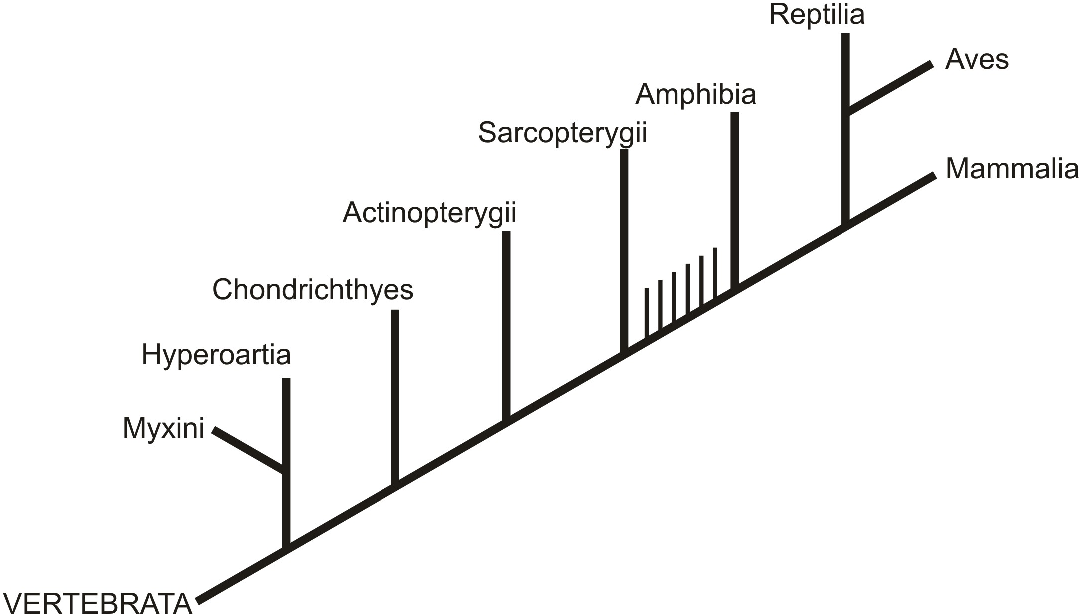
\includegraphics[width=1\textwidth]{PAU_Lamza/Lamzaorg-img001.pdf}
	\caption{A highly simplified, and ultimately wrong, phylogenetic tree of extant vertebrates that attempts to
		include only the extant classes of subphylum Vertebrata. The ‘comb’ represents the area magnified in Fig. 2. It is
		clear that one cannot map a ranked classification of extant vertebrate classes onto a valid phylogenetic tree,
		especially because of the existence of extinct groups. Specifically, it is impossible to validly represent the actual
		relationships between (paraphyletic and now obsolete) Reptilia and Aves (which nest within reptiles).}
	%\label{lamza-fig1}
\end{figure}

This is, however, yet another simplification. A more careful analysis of \textit{any }segment of the vertebrate
phylogenetic tree will reveal that in between the well-known groups there are numerous groups, usually extinct, that
would all require classes of their own, if the bordering taxa are given the rank of class -- consult Fig. 2.

\begin{figure}[h]
	\centering
	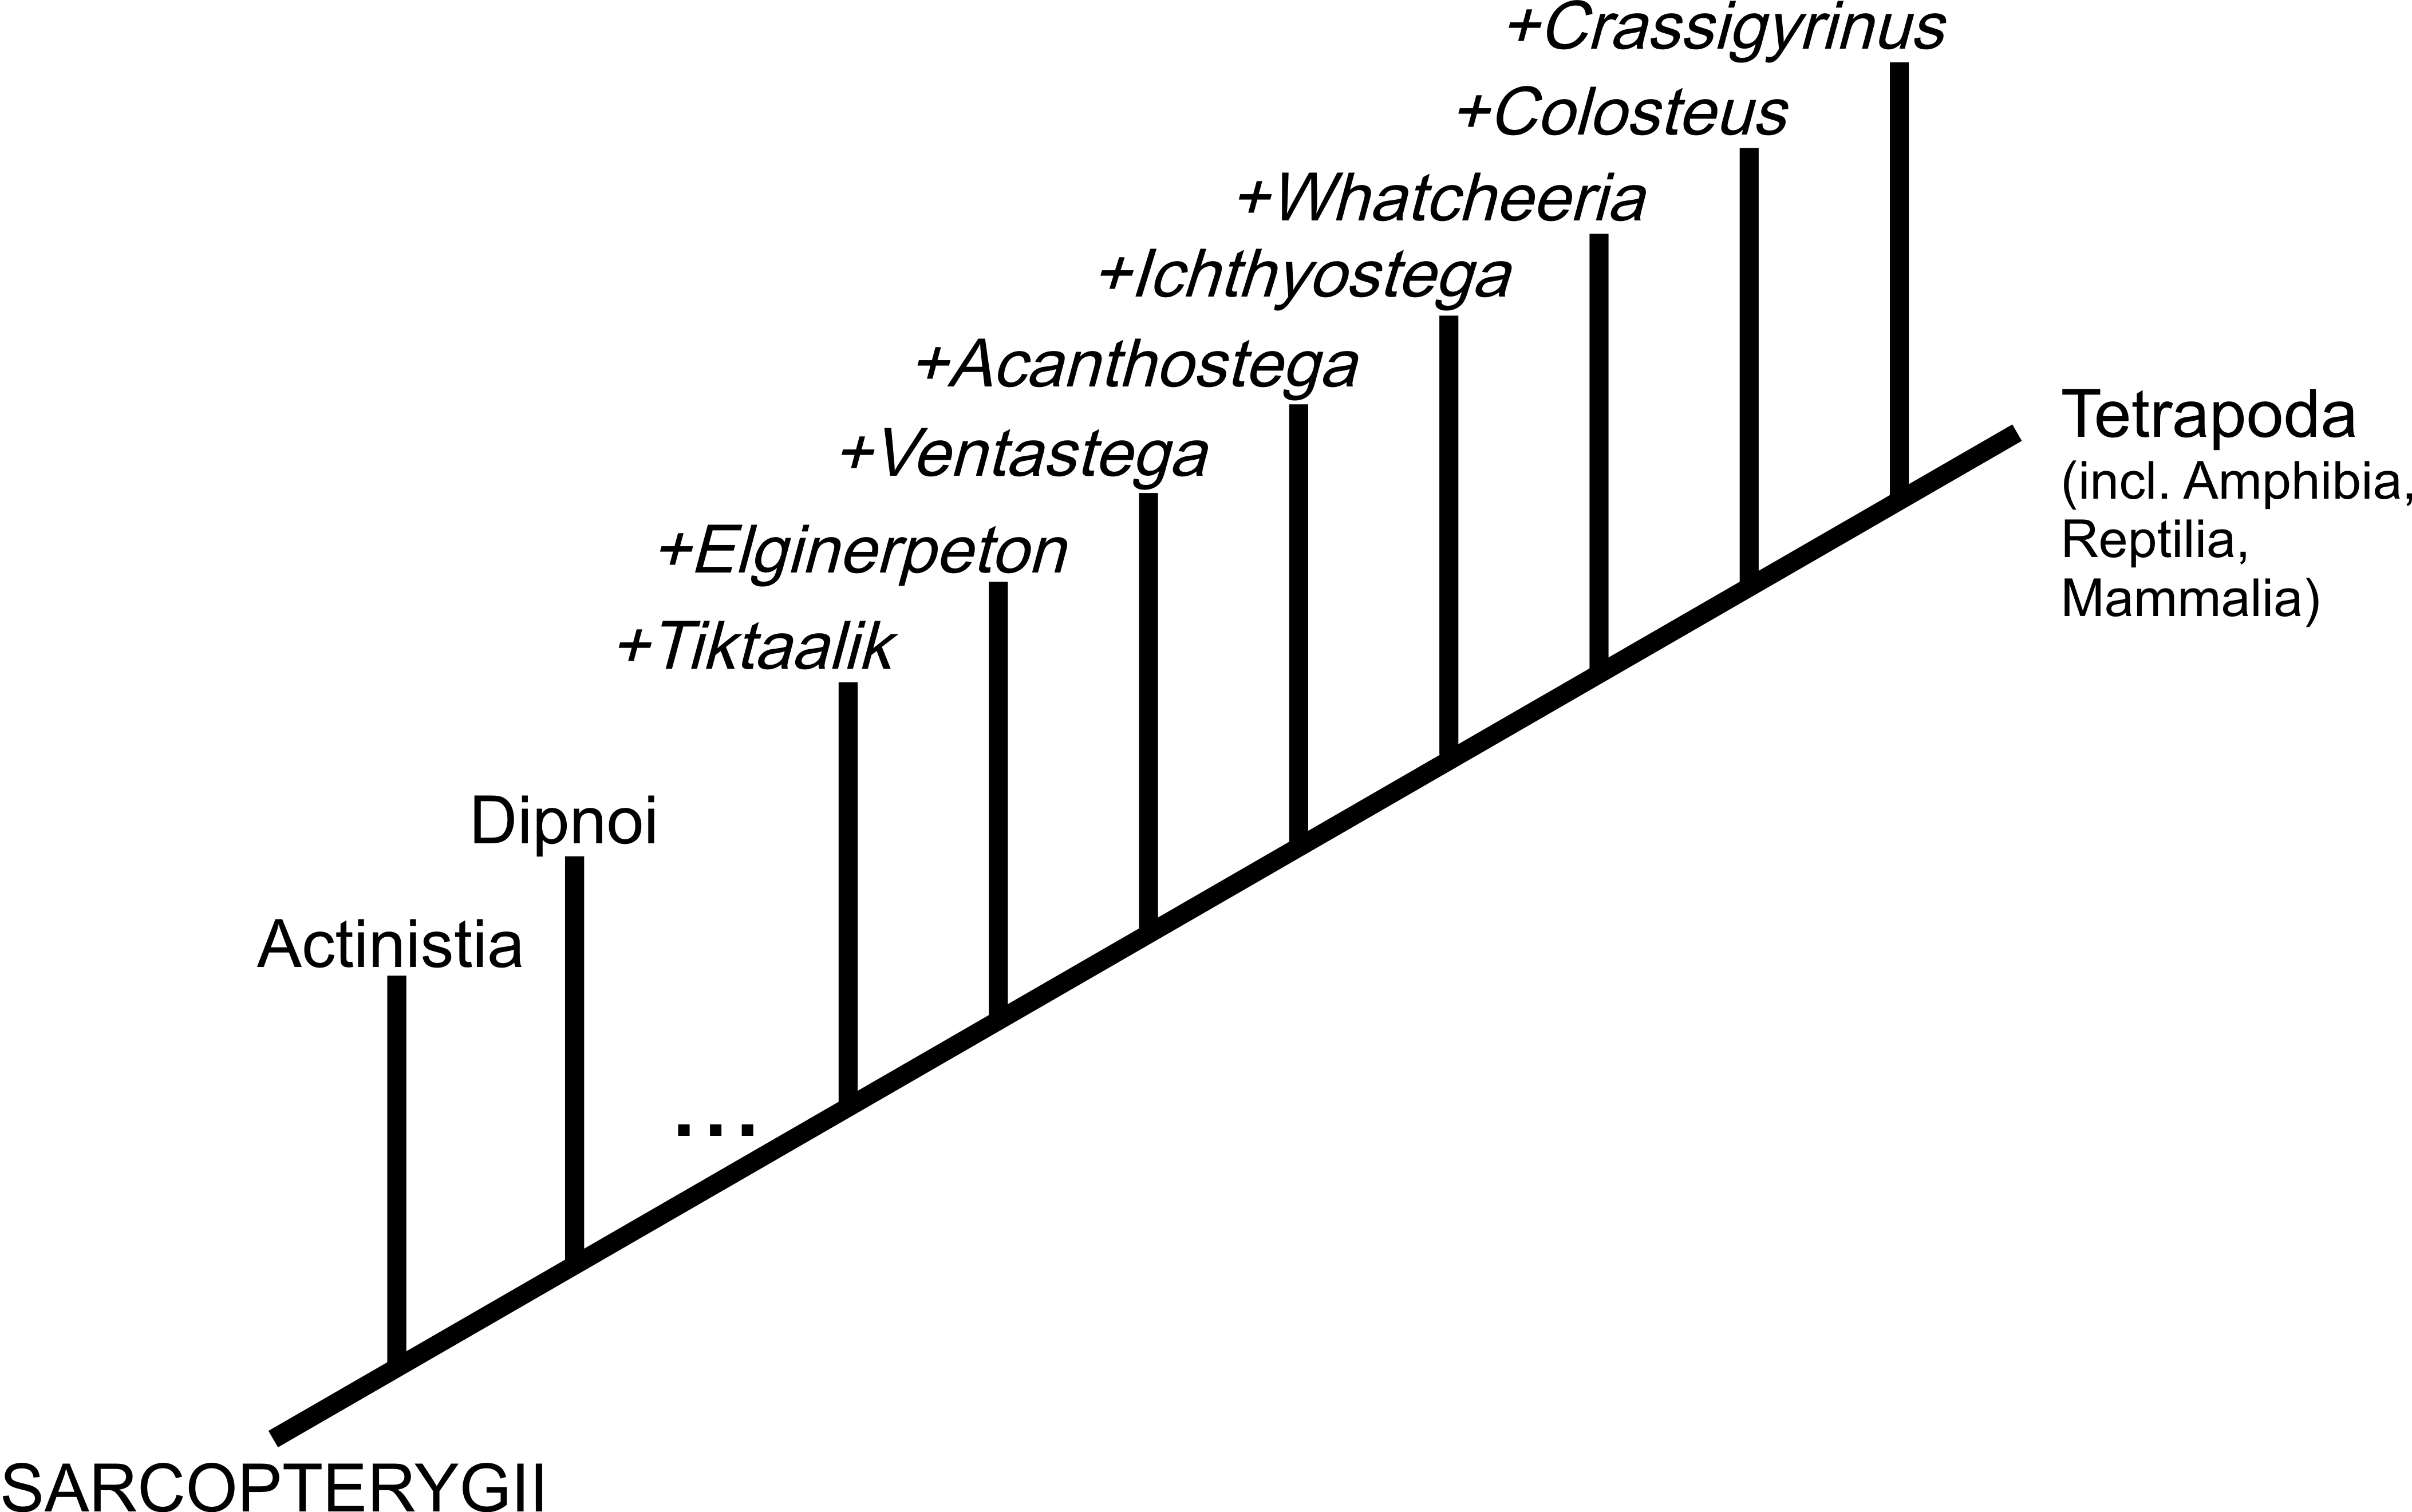
\includegraphics[width=1\textwidth]{PAU_Lamza/Lamzaorg-img002.jpg}
	\caption{A slightly more realistic representation of a segment of the vertebrate phylogenetic tree, based on
		\parencite{swartz_marine_2012}
		%\label{ref:RNDPuknxVrJnD}(Swartz, 2012)
		(with many taxa removed, most notably a large group of early sarcopterygians,
		denoted by an ellipsis). The improvement over Fig. 1 is mostly in that: a) the term Sarcopterygii is now correctly
		represented to also include all tetrapods, while in common usage, represented in Fig. 1, it refers only to coelacanths
		(which belong to Actinistia) and lungfish (which belong to Dipnoi); b) a number of extinct (marked by a cross) genera
		are presented.}
	%\label{lamza-fig2}
\end{figure}

It is clear that in order to divide the taxa listed in Fig. 2 into classes, one would have to give each genus presented
in that figure its own high-level taxon (here: most likely class). The alternative is accepting paraphyletic taxa, for
instance by grouping all stem tetrapods (Tiktaalik\ldots Crassigyrinus) in a single class. It clearly goes against
phylogenetic systematics, which is usually defended by biologists working with specific groups of organisms as the only
method of creating taxonomies that is commensurate with the theory of evolution
\parencite[see e.g.][]{williams_pursuit_2007}
%\label{ref:RNDkC4ruFguZT}(see e.g. Williams and Kociolek, 2007).

There are ways to avoid that, one of which is the so-called sequencing convention proposed by Nelson
\parencite*{nelson_phylogenetic_1972}
%\label{ref:RNDHQubFlpSOG}(1972)
and developed by Wiley
\parencite*{wiley_phylogenetics:_1981}
%\label{ref:RNDoeFoXTp1sn}(1981)
and others, which partly
automates the ranking process in various branches of the phylogenetic tree. But for new, let’s assume that we want to
hold on to strict Hennigian principles; what would be the consequences? Quite simple: the necessity to create a
complete system of monophyletic taxa, in case of vertebrates, would lead to the erection of tens, if not hundreds,
classes of vertebrates which defeats the simplifying purpose of classification. Another solution would be to erect a
large number of taxa of intermediate rank -- this has been done, for example, by McKenna \& Bell in their influential
classification of mammals
\parencite{mckenna_classification_1997}:
%\label{ref:RNDTh5Uw8JZAm}(McKenna and Bell, 1997):

\begin{longitemize}
\item class Mammalia
\begin{longitemize}
\item subclass Prototheria
\item subclass Theriiformes
\begin{longitemize}
\item infraclass +Allotheria
\item infraclass +Eutriconodonta
\item infraclass Holotheria
\begin{longitemize}
\item superlegion +Kuehneotheria
\item superlegion Trechnotheria
\begin{longitemize}
\item legion +Symmetrodonta
\item legion Cladotheria
\begin{longitemize}
\item sublegion +Dryolestoidea
\item sublegion Zatheria
\begin{longitemize}
\item infralegion +Peramura
\item infralegion Tribosphenida
\item \ldots
\end{longitemize}
\end{longitemize}
\end{longitemize}
\end{longitemize}
\end{longitemize}
\end{longitemize}
\end{longitemize}

It is worth noting that the authors of that classification are paleontologists and their system is clearly intended as
an answer to the problem of finding a proper taxonomic space for extinct groups. As a result, a staggering number of
ranks were created. In ``core Linnaean'' taxonomy classes are composed of orders, i.e. class and order are neighboring
ranks. In McKenna \& Bell’s system one will find between them: subclasses, infraclasses, superlegions, legions,
sublegions, infralegions, supercohorts, cohorts, magnorders, superorders, grandorders and mirorders. The term
``taxonomic inflation'' may thus have two meanings: the creation of an impractically large number of equally-ranked taxa
and the creation of an impractically large number of ranks.

Let’s now discuss these two alternatives in more detail.

\section{The solutions}
\vspace*{-1cm}
\subsection{Solution I: classifications with only monophyletic taxa}

As mentioned above, strictly adhering to Hennig’s prescription to accept only monophyletic taxa leads to ``taxonomic
inflation'' -- which seems to go against the aesthetic intuition of those biologists who dread the idea of splitting a
given, let’s say, phylum, into 50 classes
\parencite{cavalier-smith_revised_1998}.
%\label{ref:RNDsx8NDQDrK2}(Cavalier-Smith, 1998).

Surprisingly, the solution that has been commonly employed is to do something perhaps even more drastic: to drop
altogether the Linnaean ``logic'' of classification which is based on the simple idea that taxa of a given rank are
divided into a number of subordinate taxa of the same lower rank -- i.e. kingdoms are divided \textit{only} into phyla;
phyla are divided \textit{only} into classes; classes \textit{only} into orders etc. In other words, every order
belonging to a given phylum must \textit{also }belong to a certain class (or, in some cases, be included as
\textit{incertae sedis}, i.e. temporarily awaiting class attribution). In many modern classifications, however, there
are \textit{missing ranks}. As an example, consider the classification of vertebrates presented by the eminent
paleontologist Michael Benton in his \textit{Vertebrate Palaeontology}
\parencite[p.433nn]{benton_vertebrate_2014}
%\label{ref:RNDqnkTfPlTq8}(Benton, 2014, p.433nn):

\pagebreak%tu
\noindent$\bullet$ superclass Tetrapoda:
\begin{addmargin}[1em]{0em}
 $\circ$ family Elginerpetontidae\\
 $\circ$ \textit{Ventastega}\\
 $\circ$ \textit{Acanthostega}\\
 $\circ$ \textit{Ichthyostega}\\
 $\circ$ \textit{Tulerpeton}\\
 $\circ$ family Colosteidae\\
 $\circ$ family Crassigyrinidae\\
 $\circ$ family Whatcheeriidae\\
 $\circ$ family Baphetidae\\
 $\circ$ class Neotetrapoda [where amphibians, reptiles, birds and mammals can be found -- L.L.]
\end{addmargin}

This is a remarkable solution. Note that it clearly opposes the centuries-old tradition, formalized by Linnaeus, to
create consistent, complete hierarchies. Here we have a superclass that is composed of a single class, 5 families and 4
genera.

The missing ranks may look unsettling at first, but this convention is quickly gaining popularity, as it seems to offer
a welcome rescue from the otherwise inescapable alternatives discussed in the previous paragraph. A recent
classification of eukaryotes, published first in 2005
\parencite{adl_new_2005},
%\label{ref:RND5C0kzbt9Jm}(Adl et al., 2005),
then in a revised
form in 2012
\parencite{adl_revised_2012},
%\label{ref:RND2nC4dhq2C7}(Adl et al., 2012),
employs precisely that methodology. Note that this is an
extremely well-respected classification, created by a consortium that includes world-class experts in eukaryotic
diversity (such as Alastair Simpson or Sergei Karpov). The pair of papers is now amongst the most oft-quoted articles
in the field, which means in practice that it is now a point of departure in any discussion of eukaryote
classification.

In both papers the ranks are altogether dropped. Curiously, the taxa are presented in a semi-ordered hierarchical form
where subordinate taxa are given more black dots. For instance, in the earlier paper
\parencite{adl_new_2005}
%\label{ref:RNDFR1OTfHJvd}(Adl et al., 2005)
the group Opisthokonta is presented as follows (numerous taxa have been omitted):

\noindent OPISTHOKONTA\\
$\bullet$ Fungi\\
$\bullet\bullet$ Basidiomycota\\
$\bullet\bullet$ Urediniomycetes\\
$\bullet\bullet$ Ustilaginomycetes\\
$\bullet\bullet$ Ascomycota\\
$\bullet\bullet$$\bullet$ \textit{Neolecta}\\
$\bullet\bullet$$\bullet$ Taphrinomycotina\\
\ldots\\
$\bullet$ Mesomycetozoa\\
$\bullet\bullet$ Aphelidea\\
$\bullet\bullet$ \textit{Corallochytrium}\\
$\bullet\bullet$ \textit{Capsaspora}\\
$\bullet\bullet$ Ichthyosporea\\
$\bullet\bullet$ \textit{Ministeria}\\
$\bullet\bullet$ Nucleariida\\
$\bullet$ Choanomonada\\
$\bullet$ Metazoa\\
$\bullet\bullet$ Porifera\\
$\bullet\bullet$$\bullet$ Silicispongia\\
$\bullet\bullet$$\bullet\bullet$ Hexactinellida\\
$\bullet\bullet$$\bullet\bullet$ Demospongiae (\ldots)

Let’s note a few properties of this classification method. First of all, the four main groups of Opisthokonta
(the ones with a single dot, i.e. fungi, mesomycetozoans, choanomonads and animals) are, to the best of current
phylogenetic knowledge, monophyletic. This makes them perfect for the role of taxa in an openly Linnaean system, that
is at the same time in line with Hennig’s rules of phylogenetic classification. The taxa with the same number of dots,
however, represent radically different ranks in previously published classifications. The group Mesomycetozoa, as
presented here, is composed of three genera (\textit{Corallochytrium}, \textit{Capsaspora} and \textit{Ministeria}),
two classes (Aphelidea and Ichthyosporea) and one order (Nucleariida). One might of course erect classes for all of
them, which however, often leads to taxonomic inflation, as mentioned in the previous section.

Let’s now specifically discuss the problem of kingdoms. If we hold on to the idea that equal ``ranks'' in the
classification by Adl \textit{et al.} should be given equal Linnaean ranks, we would be forced to create two additional
kingdoms Choanomonada and Mesomycetozoa, that would be placed alongside Fungi and Metazoa/Animalia in the, most likely,
superkingdom Opisthokonta (plus other kingdoms in other superkingdoms). That is, in fact, a fairly popular point of
view, expressed for instance by Tedersoo
\parencite*{tedersoo_proposal_2017},
%\label{ref:RNDXAoIqIPayD}(2017),
who includes kingdoms Choanoflagellozoa
(essentially synonymous with Adl \textit{et al.}’s Choanomonada) and Ichthyosporia (Ichthyosporea is a synonym of
Mesomycetozoa in many classification systems). It is worth noting that Tedersoo’s system might be thought of as a good
demonstration of what happens if one attempts to create a Linnaean system adhering to Hennigian constraints, based on
modern understanding of eukaryotic phylogeny (the classification by Adl \textit{et al.} is listed by Tedersoo as one of
his main sources of information). The result? His system has 32 eukaryotic kingdoms. Let’s cite his own opinion on that
fact: ``In the proposed classification, the erection of 32 eukaryote kingdoms certainly catches and, perhaps, scratches
the eye. I found adoption of multiple kingdoms necessary to follow the monophyly principle […].''
\parencite[p.8]{tedersoo_proposal_2017}
%\label{ref:RNDP7J0D4JTk6}(Tedersoo, 2017, p.8)

Note that Adl \textit{et al. }themselves stand \textit{against }such practices, calling such artificially created
higher-level taxa ``superfluous''
\parencite[p.430]{adl_revised_2012},
%\label{ref:RNDTkKC0gomXM}(Adl et al., 2012, p.430),
therefore openly arguing for
classification with missing taxa.

\subsection{Solution II: classifications with paraphyletic taxa}

The most vocal contemporary proponent of that solution is probably Thomas Cavalier-Smith, a controversial figure among
microbiologists, who, however, is at the same time undoubtedly one of the most influential personas in the field of
eukaryotic systematics. His contributions include the early recognition, and naming, of Excavata, Opisthokonta,
Rhizaria and Chromista -- all of them being now largely accepted, and the latter three: most likely monophyletic,
mega-grouping of eukaryotes. In his proposed classification of life (with six kingdoms)
\parencite{cavalier-smith_revised_1998}
%\label{ref:RNDScaXMIFqT5}(Cavalier-Smith, 1998)
there is a long section on ``philosophical preliminaries'', where the
necessity for admitting paraphyletic taxa is forcefully defended. His two main arguments against the Hennigian
requirement to limit taxa to clades are as follows:

1) It leads to instability. Each new discovery in biology -- be it a paleontological or molecular novelty, or simply the
discovery of a new species or a reinterpretation of anatomical data -- may lead to the reassessment of a monophyletic
taxon as paraphyletic, which would force the biologists to update classification systems. In practice it would mean
hundreds, if not thousands, of revisions every year.

2) It is not practical. Let’s quote Cavalier-Smith himself: ``Whether a taxon is paraphyletic or not is irrelevant to its
validity as a taxon. It is also irrelevant to many of the uses to which classifications are put, such as arranging
specimens in a museum, organising the chapters in a biology textbook, or providing a convenient label, e.g. bacteria or
fungi, for a group of similar organisms.''
\parencite[p.212]{cavalier-smith_revised_1998}
%\label{ref:RNDUlTuwI9YEO}(Cavalier-Smith, 1998, p.212)

As a result, Cavalier-Smith for about two decades has become an active opponent of Hennigian classification, especially
in the field of microbiology. Every year or two he proposes a new system of classification, sometimes general, most
often specific to a group of eukaryotes
\parencite{cavalier-smith_phagotrophic_2002,cavalier-smith_early_2013,cavalier-smith_higher_2016},
%\label{ref:RNDtoAIslWhri}(see e.g. Cavalier-Smith, 2002, 2013, 2016),
usually
being a carefully crafted compromise between contemporary phylogenetic knowledge and practicality. His 1998 system
\parencite{cavalier-smith_revised_1998}
%\label{ref:RNDJbJ6dU4tG1}(Cavalier-Smith, 1998)
has six kingdoms:

\begin{longitemize}
\item empire/superkingdom Prokaryota*
\begin{longitemize}
\item kingdom Bacteria* [note: Archaebacteria are to be found here, as an infrakingdom]
\end{longitemize}
\item empire/superkingdom Eukaryota
\begin{longitemize}
\item kingdom Protozoa*
\begin{longitemize}
\item subkingdom Archezoa*
\item subkingdom Neozoa*
\end{longitemize}
\item kingdom Animalia
\item kingdom Fungi
\item kingdom Plantae
\item kingdom Chromista
\end{longitemize}
\end{longitemize}
All openly paraphyletic (``almost certainly paraphyletic'' in his own words) taxa are marked with an asterisk. It is
interesting to note that, while Cavalier-Smith openly opposes Hennigian phylogenetic systematics, his ``illegal''
taxonomies are highly popular. A quick look into any contemporary paper on eukaryotic systematics will reveal a number
of high-level taxa formally defined by Cavalier-Smith, many of them known or suspected to be paraphyletic. The reason
is simple: his classifications are extremely convenient, because they are invariably composed in such a way as to
include only a minimal number of taxa \textit{and} ranks which are \textit{usually }monophyletic, but sometimes are
paraphyletic if that makes for a convenient system. The reader is referred to the above-cited paper (Cavalier-Smith,
1998) where his philosophy of biological classification is explained in detail.

On a side, and probably more personal, note: the zoologists reading this paper may find it interesting to go through his
proposed classification of the animal kingdom
\parencite[pp.235–237]{cavalier-smith_revised_1998}
%\label{ref:RNDayLTgHPurs}(Cavalier-Smith, 1998, pp.235–237)
which offers,
in the opinion of the author of this paper, a refreshing look at the list of animal phyla. As currently recognized,
there is somewhere around 30-35 phyla -- consult any modern textbook on zoology -- that only recently began to be grouped
into a few large monophyletic groups, such as Spiralia, Ecdysozoa or Deuterostomia. Other than that, there is a
confusing diversity of tiny phyla, most of them unknown to the general public: how many non-zoologists know of
Kinorhyncha, Loricifera, Gnathostomulida (jaw worms) or Acanthocephala (spiny-headed worms)? Cavalier-Smith groups all
animals into 22 phyla -- still a long list, but, especially with the aid of his clear, succinct diagnoses, is much more
manageable. The classification includes some, but rather few, paraphyletic taxa.

\subsection{Solution III: abandon classification systems}

The third solution would be to run away from the problem, so to speak, and refrain from explicitly writing down
classifications, and discuss biological diversity through phylogenetic trees only. This has been proposed from time to
time by certain scientists and philosophers (the proposal has been reviewed and critiqued by Michael Benton
\parencite*{benton_stems_2000}).
%\label{ref:RNDvl4WtKWtke}(2000)).
While reading biological literature, one finds this sentiment expressed from time to
time, especially by specialists working with rapidly changing classification systems. There is a fascinating, heated
dialogue that ensued during the 1970 First International Conference on Ephemeroptera, recorded in this conference’s
proceedings
\parencite[pp.151–154]{peters_proceedings_1973},
%\label{ref:RNDKBHKSFREeT}(Peters and Peters, 1973, pp.151–154),
where a group of entomologists become
increasingly frustrated by their inability to create a classification system based on the otherwise clear phylogenetic
evidence presented by one of the participants
\parencite{edmunds_jr_critical_1973}.
%\label{ref:RNDRwD3oy2Fl1}(Edmunds Jr, 1973).
In fact, all the problems
discussed in this paper with regard to higher ranks are mentioned during that discussion, which is about families,
subfamilies and genera of Ephemeroptera, which makes for a great read.

There are at least two large groups in biology that have abandoned updating the classification of the organisms they are
working with: botanists working with flowering plants and malacologists.

In the first case, one would be hard-pressed to find a recent authoritative classification of flowering plants, because
the focus of the communal effort has long been the creation of better and better phylogenies, not taxonomies. The
Angiosperm Phylogeny Group regularly publishes the new view on plant phylogeny, employing formal taxa only to the level
of order %\label{ref:RNDly7gwmyvG1}(see e.g. Chase et al., 2016). All the higher-rank taxa are abandoned, and no
higher-rank taxonomies are officially accepted by APG.

The exactly same process had happened in the field of malacology, where for years there were no formal definitions of
gastropod taxa above the level of superfamily
\parencite[see][]{bouchet_classification_2005}.
%\label{ref:RND5saL769IKK}(see Bouchet and Rocroi, 2005).
Interestingly,
the situation visibly upset some of the workers in the field who started spontaneously grouping the newly defined
families and superfamilies into orders, those into superorders, subclasses etc. Last year in a revision of the 2005
classification
\parencite{bouchet_revised_2017},
%\label{ref:RNDSnxh8fRQNP}(Bouchet et al., 2017),
the authors surrendered and included higher-ranked
taxa, although the system is now very ``messy'': it includes numerous intermediate-level ranks that correspond to the
unranked clades in the previous classification -- there are classes, subclasses, infraclasses, cohorts, subcohorts,
superorders, orders, suborders and infraorders in the system, plus a handful of openly paraphyletic ``grades''. The
struggle of malacologists to bring back Linnaean classification into the world of Hennigian unranked lists à la Adl
\textit{et al.} leads to exactly the same problems that were discussed in the previous sections.

The case of gastropod classification illustrates, however, that even specialists working in very narrow fields need
balanced ranked classification systems. It is not only for the purposes of educating the young, writing books or
organizing museum expositions that we need neat, logical classifications with no missing ranks and a small number of
distinctive, easy to remember taxa. The specialists need them too. The option to abandon classification systems seems
to be not viable, especially that it is both trivial and tempting to create a list of clades from a phylogenetic tree,
adding ranks to some or all taxa, which would be a \textit{de facto} classification, just like Benton did in his
\textit{Vertebrate Palaeontology}.

\section{Summary}

Our increasing knowledge of biodiversity, especially in the case of microbiology, both prokaryotic and eukaryotic, will
inevitably lead to the escalation of the problems presented in this paper. Because it doesn’t seem plausible that
classification systems will be altogether abandoned (which would leave us only with phylogenetic trees, sometimes
presented as unranked lists), it seems that we must somehow solve the problem of creating classification systems in the
times of abundant phylogenetic data.

Broadly speaking, there seem to be two directions that one might take: 1) to follow phylogenetic data to the letter; 2)
to follow intuition and convenience. Simply put, the option 1) would mean having only proper monophyletic taxa, but a
highly impractical system; and the option 2) would mean having also paraphyletic taxa \textit{and} a system that is
practical.

In the special case of eukaryotic kingdoms, the first route would lead to a revolution in biological classification of
life and numerous kingdoms currently unknown to the general public would be introduced
\parencite{tedersoo_proposal_2017},
%\label{ref:RND3uML7k6B2X}(Tedersoo, 2017),
such as Oxymonada, Breviatea or Filasteriae, that would now be listed
alongside plants, animals and fungi as ``major types of life''. Alternatively, one might drop the traditional kingdoms
altogether and define the currently recognized eukaryotic ``supergroups''
\parencite[e.g.][]{keeling_tree_2005}
%\label{ref:RNDsc7VI9vP7w}(e.g. Keeling et al., 2005)
as kingdoms, and what we know recognize as kingdoms would have to be downranked into subkingdoms or
``microkingdoms''
\parencite{pawlowski_new_2013}.
%\label{ref:RNDAlF3xlGnxL}(Pawlowski, 2013).
This would be the resulting classification:

\begin{itemize}
\item kingdom Excavata
\item kingdom Amoebozoa
\item kingdom Opisthokonta (incl. fungi and animals)
\item kingdom Archaeplastida (incl. plants)
\item kingdom Rhizaria
\item kingdom Alveolata
\item kingdom Heterokonta
\end{itemize}
Obviously, this would \textit{not} solve the problem, if one would stubbornly keep on sticking to Hennigian rules. First
of all, Excavata may be paraphyletic
\parencite{he_alternative_2014},
%\label{ref:RNDd85mwMFAal}(He et al., 2014),
in which case we would have to split
it into monophyletic groups, resulting in a classification system alike to this:

\begin{itemize}
\item kingdom Euglenozoa (former Excavata)
\item kingdom Heterolobosea (former Excavata)
\item kingdom Jakobea (former Excavata)
\item kingdom Metamonada (former Excavata)
\item kingdom Amoebozoa
\item kingdom Opisthokonta (incl. fungi and animals)
\item kingdom Archaeplastida (incl. plants)
\item kingdom Rhizaria
\item kingdom Alveolata
\item kingdom Heterokonta
\end{itemize}
Secondly, there is at least a dozen groups of eukaryotes that don’t fit neatly into any of the supergroups, including
\textit{Tsukubamonas} and \textit{Malawimonas}, Cavalier-Smith’s Varisulca, Apusozoa, but also much better-known groups
such as Cryptophyta or Haptophyta. Consequently, in Tedersoo’s system, there \textit{are} kingdoms Malawimonada,
Tsukubamonada, Apusozoa, Cryptista and Haptista which brings us to square one. Obviously, replacing traditional
kingdoms with eukaryotic supergroups is \textit{not }a solution.

The second option -- to retain the general structure of the present classification of life into kingdoms -- is not fully
satisfactory, either, because the old kingdom Protozoa is now known to be a large, highly structured group that
deserves proper recognition and can’t be rightfully treated as an unstructured bunch of ``amoeba and such''
\parencite[see][]{patterson_diversity_1999}.
%\label{ref:RNDBkv0g8EycM}(see Patterson, 1999).
Its representatives have very little in common with each other and
include multicellular forms similar to fungi (mycetozoan slime molds, acrasids) and plants (brown algae), single-celled
large predatory heterotrophs (ciliates), intracellular parasites (kinetoplastids) and endosymbionts (syndineas);
colonial filtrators (choanoflagellates), multinucleate ``superamoebae'' (labyrinthulomycetes) and tens of other forms.
Small steps, such as Cavalier-Smith’s proposal for the kingdom of Chromista, might be seen a sign of a more
conservative process of a slow, incremental change, not dictated by blind adherence to formalized ideals, but rather by
educational values.

At the moment it is uncertain which approach will dominate, but it’s clear that creating a top-level classification of
life congruent with our contemporary knowledge of eukaryote phylogeny will require us to resign from at least some
philosophical principles of biological systematics.

\end{artengenv}


\addtocontents{toc}{\protect\pagebreak}


\sekcja{Klasycy: teksty-komentarze}{Classics: texts and commentaries}
%\sekcja{Z lektury klasyków}{Learning from the classics}

\begin{artengenv}{Michael Heller}
	{How is \textit{philosophy in science} possible?}
	{How is {\pagname{philosophy in science}} possible?}
	{How is {\tocname{philosophy in science}} possible?}
	{Translated by Bartosz Brożek and Aeddan Shaw\edtfootnote{In this edition some quotations have been replaced by the translations of their original sources (if available). The references have been adjusted to the standards of the journal.}\label{heller-start}}
	{The Michael Heller's article entitled ``How is \textit{philosophy in science} possible?'' was originally published in Polish in 1986
		\parencite[see][]{heller_jakmozliwa_1986} and then translated into English by Bartosz Brożek and Aeddan Shaw and published in 2011 in the collection of essays entitled \textit{Philosophy in Science. Methods and Applications} \parencite{heller_howpossible_2011}. This seminal paper has founded further growth of the `philosophy in science' and become the reference point in the methodological discussions, especially in Poland. On the 40\textsuperscript{th} anniversary of \textit{Philosophical Problems in Science} we wanted to make this paper freely available to the international public by reprinting its English version. In this issue it is followed by two additional articles-commentaries (by Paweł Polak and Kamil Trombik).}
	{philosophy in science, philosophy of science, metaphilosophy, interdisciplinary research, science and religion, analytic philosophy.}



\section{Introduction}


\lettrine[loversize=0.13,lines=2,lraise=-0.05,nindent=0em,findent=0.2pt]%
{P}{}hilosophy in science' grew out of practice.\label{heller-out-of} Its most significant example is the phenomenon of the `philosophizing
physicists'. And even though the philosophical reflection of the representatives of the empirical sciences often falls
short of the professional philosophical standards, it does not change the fact that the sciences are filled with
philosophical contents.

\AddToShipoutPictureFG*{% Add <stuff> to current page foreground
	\put(\LenToUnit{22mm},\LenToUnit{168.5mm}){\begin{minipage}[t][23mm][t]{\textwidth}`\end{minipage}}%
}%

In the recent years in the Polish philosophical literature such terms as `philosophical issues in science' have
appeared on the covers of several publications.\footnote{Cf. \textit{Zagadnienia Filozoficzne w Nauce}, a periodical
published in Kraków since 1978; see also
\parencite{heller_zagadnienia_1980}.
%\label{ref:RNDeyUVXQ9KCX}(Heller, Lubański and Ślaga, 1980).
} The English
`philosophy in science', through its contrast with, and similarity to `philosophy of science', has been `sanctioned' in
the title of a new periodical.\footnote{\textit{Philosophy in Science} is published by Pachart Publishing House,
Tuscon. The first volume appeared in 1983.} The paper by W.H. Stoeger, published in the first volume of
\textit{Philosophy in Science}, may be considered a manifesto of the editorial board, as well as an attempt to provide
a theory of `philosophy \textit{in} science'.\label{heller-stoeger}

I am against any planning what kind of philosophy should be practised, i.e. determining \textit{a priori} the method
of analysis and its consequent application. It is more natural when the methodological reflection follows the period of
abundant, sometimes instinctive or even chaotic research in a new discipline. I believe, however, that the time has
come for an attempt to systematize what \textit{de facto} is `philosophy in science'.\label{heller-defacto}


\section{Philosophy in science and philosophy of science}

Among the philosophers of nature (in particular those belonging to the neo-thomistic school) there is a commonly
accepted doctrine of the non-intersecting planes. Generally speaking, it says that philosophical cognition lies at a
totally different epistemological plane than the empirical sciences; they use different methods and operate with
mutually untranslatable languages.\footnote{This is a kind of philosophy advanced in two books:
	\parencite{mazierski_prolegomena_1969,klosak_z_1980}.
%\label{ref:RNDDukAXvxyUz}(Mazierski, 1969; Kłósak, 1980).
Both these authors seem to see the need for the mutual
influences of philosophy and the sciences and develop subtle distinctions in order to open the way for such influences
despite the non-intersecting planes.} In order to justify this view the theories developed within the contemporary
methodology are cited. It is sometimes tempting to say that the major motive behind such stances is to safeguard one's
philosophy against any conflict with the sciences, as well as the theoretical justification of one's incompetence in
the sciences.

The proponents of the two planes doctrine may protest against the `philosophy in science' project as
methodologically flawed and epistemological nonsense, an attempt at a comparison of the incomparable. I recall those
objections not in order to dismiss them (the best way to reply to them is through the results already obtained in the
`philosophy in science' field), but to underline the relationship between `philosophy in science' and philosophy of
science. It is obvious that any philosophizing which is open for the dialogue with the empirical sciences must take
into account their achievements. Otherwise it would be subject to the objection of anachronism. It is equally difficult
to reject the claim that there exist serious differences between the `cognitive plane' of the empirical sciences and
some philosophical currents. I do not believe, however, in any strict isolationism: of the philosophy in relation to
the sciences, or \textit{vice versa}. The methodological bans will be breached anyway, and it is often through the
violation of the received canons that new paradigms emerge, i.e. some progress is made in our attempts to understand
the world: the two non-intersecting planes may turn out to be elements of the same stratification of a more-dimensional
space.

`Philosophy in science' has \textit{de facto} been practised from the beginnings of the empirical sciences. For
example, looking at the Newton's oeuvre, it is difficult to determine whether it is a case of science in philosophy, or
already of philosophy in science.\label{heller-newton} Thus, an attempt to categorize \textit{ex post }the problems of `philosophy in
science' is possibly realizable; however, in face of the richness of this problematic, I shall concentrate on a
succinct analysis of three exemplary issues. Although they do not exhaust the content of `philosophy in science', they
remain typical examples so that they enable to reconstruct its nature and methods. In what follows I shall present (A)
the influence of the philosophical ideas on the development and evolution of scientific theories; (B) the traditional
philosophical problems intertwined with empirical theories; (C) philosophical reflection over some assumptions of the
empirical sciences.\label{heller-three-points}


\section{The influence of philosophical ideas on the development and evolution of scientific theories}


Empirical science originated through the separation from the old, all-embracing philosophy and still bear the
imprint of this origin. Contemporaneously, various philosophical ideas often serve as an inspiration for developing new
conceptions in the empirical sciences. However, many methodologists defend the `purity' of science by introducing the
well-known distinction: indeed, in the context of discovery philosophical ideas often influence the development of
science, however it is not their role only---other factors, even irrational ones, may be influential in the process of
arriving at new discoveries; on the other hand, in the context of justification, i.e. the sphere of the proper
science-creating activities, philosophy has no bearing---it is an `alien body', effectively eliminated by the built-in
mechanisms of science. It is the disregard for this distinction that led to the phenomenon of the `philosophizing
physicists'---the representatives of the empirical sciences who, wrongly taking the context of discovery for the
discovery itself, believe to have something philosophically interesting to say, while in fact they reveal only their
psychological associations.

In the recent years, the distinction between the two contexts has been severely criticized. A case in point is the
following passage from Stefan Amsterdamski's study: %
%Zastąpiłem fragmentami z tłumaczenia książki Amsterdamski. 
%Oryginał z tłumaczenia Brożek\&Shaw: „Metaphysics, myths, prejudices are in a way an immanent element of science on par with the fact we try to incorporate into a rational reconstruction. Neoplatonic philosophy of Kepler or Copernicus constituted an aspect of the rational order of the universe they were trying to uncover in the same sense the strictly empirical statements of their astronomical systems did.'' (Amsterdamski, 1973, p.99)
%nieznany
%June 28, 2019 11:54 PM

\myquote{
Metaphysics, myths or superstitions are in some manner as immanently a part of science as the facts which we attempt to
include into the rational reconstruction. The neoplatonic metaphysic of Kepler and Copernicus were as much an element
of the rational organization of the universe which they attempted to reconstruct as the strictly empirical statements
of their astronomic systems
\parencites[p.99]{amsterdamski_miedzy_1973}[pp.65--66]{amsterdamski_between_1975}.
%\label{ref:RNDU9z9ka2JPW}(Amsterdamski, 1973, p.99, 1975, pp.65---66)
}
To put it more
succinctly: %
%Zastąpiłem fragment: „Science thus always comprises not only the claims about the studied universe, but also the assumptions pertaining to the nature of the subject who practices science.'' (Amsterdamski, 1973, p.100) 
%nieznany
%June 28, 2019 11:55 PM
\myquote{
Therefore, science consist not only of statements about the universe under study, but also of assumptions about the
knowing subject
\parencites[p.100]{amsterdamski_miedzy_1973}[p.66]{amsterdamski_between_1975}.
%\label{ref:RNDhNkCU0uqR3}(Amsterdamski, 1973, p.100, 1975, p.66)
}
If this line of argument is sound,
`philosophy of science' is simply a part of the science itself.

It is worth underlining, that the psychological or sociological accounts of the philosophy of science---which have
recently gained in strength and prestige---almost completely dispense with the distinction between the `logic of science'
and the `external circumstances' of that logic
\parencites{amsterdamski_miedzy_1983}{amsterdamski_between_1992}[cf.][]{zycinski_jezyk_1983_in_hell}.
%\label{ref:RND1eO94kZzna}(Amsterdamski, 1983, 1992; cf. Życiński, 1983).
It is not my goal to engage in a philosophical discussion. However, I personally consider the distinction between the
context of discovery and the context of justification useful under the condition that it is  understood in a flexible
way, which paves the way to a gradual passage from one  context to the other. All in all, the impossibility of drawing
a sharp demarcation line between `inspirations' and `justification' is a sufficiently strong argument in favour of the
`philosophy in science'.

Another conception of the contemporary methodology which clearly points towards some philosophical elements in
science is the so-called thematic analysis, proposed by Gerald Holton \label{ref:RNDQaGpAxlOZj}(cf. Holton, 1998). He
believes that in many concepts, methods, claims and hypothesis of science there are certain elements he calls
\textit{themata}, which as if from hiding influence or even determine the development of new scientific ideas.
\textit{Themata} often come in pairs (of opposites), sometimes in triplets, and have surprising durability over the
centuries---they are capable of surviving many scientific revolutions. Here are some examples of \textit{themata}:
unity---multiplicity; determinism---indeterminism; continuity---discontinuity; symmetry; invariance, complementarity, etc.
Holton is surprised with the relatively small number of \textit{themata}---in physics he identified some 100
thereof---and underlines their interdisciplinary and philosophical character. \textit{Themata} may constitute the
pivotal ideas for the studies in the history of science, but considered from the perspective of their philosophical
load they are nothing else but `philosophy in science'.


\section{Traditional empirical problems intertwined with empirical theories}


One can enumerate a number of such problems or rather clusters of problems. Here, I shall limit myself to examples
pertaining to time and space. It would be difficult to find a philosophical system that has nothing to say about time
and space; and it would be difficult to identify a relatively comprehensive contemporary physical theory that would
assume no theses pertaining to time and space. A classical objection against such bonding of philosophy with empirical
theories consists in stressing the fact that any doctrine which `migrates' from philosophy to the `specialized'
disciplines loses irrevocably its philosophical character, and the only thing that speaks to its philosophical origins
are words, which---even though they sound the same---have completely changed their old meanings. As elsewhere, the doctrine
of planes guards here the purity of philosophy. As I remarked earlier, it is not my goal to fight this doctrine; I
would like to show, however, that philosophy exercises much more direct influence over the development of empirical
theories than granted by the traditional wisdom.

Sometimes, in philosophy a view or a complex set of ideas---we shall say: a doctrine---is established which becomes a
kind of paradigm or a research programme for one or more empirical theories. It so happens that philosophical paradigms
are incorporated into some empirical theories (possibly in violation of the rule that forbids trespassing from one
`plane' to the other, while changing its `meaning content'); but it happens also that a paradigm resists all such
attempts, which leads to partial effects or side-effects only. When an empirical theory succeeds in realizing such a
philosophical programme, one may say that the given empirical theory is a model of the given philosophical doctrine.
The conception of empirical models of philosophical doctrines is still awaiting a more thorough analysis. Below, I
confine myself to examples pertaining to the philosophy of space and time.

In the famous \textit{Scholium} at the beginning of his \textit{Philosophiae Naturalis Principia Mathematica},
Newton formulated a philosophical doctrine of the absoluteness of time and space:

\myquote{
Absolute, true, and mathematical
time, of itself, and from its own nature flows equably without regard to anything external, and by another name is
called duration.---Absolute space, in its own nature, without regard to anything external, remains always similar and
immovable
\parencite[Scholium B]{newton_philosophiae_1687}.
%\label{ref:RND5nqR34354w}(Newton, 1687, Scholium B)
}

Today one would say that these definitions functioned
within the context of discovery of the classical mechanics. It is certainly true, but this was not their only role. It
was Newton's intent to incorporate the doctrine of the absolute time and space into the new mechanics. Newton himself,
as well as generations of physicists that followed him, believed that he had succeeded in doing so. However, a careful
analysis, with the use of the contemporary mathematical tools, reveals that---indeed---the absolute time plays an important
role in the structure of the classical mechanics, but the structure does not include an element that would correspond
to the philosophical intuitions pertaining to the absolute space
\parencite[pp.57--81]{raine_science_1981}.
%\label{ref:RND4xun9zJHBa}(cf. Raine and Heller, 1981, pp.57---81).
Thus, one must carefully distinguish between Newton's own views concerning space and time and the structure
of space and time presupposed by the Newtonian mechanics. The fact that Newton's views are incompatible with the
`views' of his mechanics is clear evidence that philosophical ideas are active not only in the contexts of discoveries,
but are also intimately linked to the history of justifications of scientific theories.

To sum up this stage of our reflection, one may succinctly say: the classical mechanics is a physical model of the
philosophical doctrine of the absolute time; however, it is not a physical model of the doctrine of the absolute
space.\footnote{In connection to the problem of the logical structure of the classical mechanics analysed with the use
of the contemporary mathematical techniques, it is also worth mentioning two studies
\parencite{friedman_foundations_1983,torretti_relativity_1983}.
%\label{ref:RNDIYv6tEO5va}(Friedman, 1983; Torretti, 1983).
}

The `other side' of this story is equally instructive. Long before Newton there was known a philosophical doctrine
rival to the conception of the absolute time and space. Its most famous incarnation was formulated by Leibniz:

\myquote{
As for
my own opinion, I have said more than once, that I~hold \textit{space} to be something \textit{merely relative}, as
\textit{time} is; that I hold it to be an \textit{order of coexistences}, as time is an \textit{order of successions}
\parencite[p.57]{leibniz_mr._1717}.
%\label{ref:RNDRSL4adjdiS}(Leibniz, 1717, p.57)
}

Despite the clear attractiveness of the Leibnizian philosophy of time
and space, it belonged the philosophy textbooks only till the development of  the theory of relativity
\parencite[cf.][]{heller_physicists_1975}.
%\label{ref:RNDn9tYnMyJ9c}(cf. Heller and Staruszkiewicz, 1975).
The obvious reason for this was that neither Leibniz
nor any of his followers managed to create a physical model of the philosophical doctrine of the relative character of
space and time
\parencite[cf.][]{raine_science_1981}.
%\label{ref:RNDlDZpjVPVrx}(cf. Raine and Heller, 1981).
There is a deeply rooted conviction that such a
model was provided by the general relativity theory. This conviction proved essentially wrong,\footnote{The problem is
more subtle than the above considerations suggest. One would need to identify at least several senses of `relational'
and `absolute'. There is no place in this essay to go into the details, thus I recommend the cited works
\parencite{raine_science_1981},
%\label{ref:RNDRTE2UAbuq1}(Raine and Heller, 1981),
as well as
\parencite{friedman_foundations_1983}.
%\label{ref:RNDf9yHzW0dHY}(Friedman, 1983).
} but the
analysis led to a new, interesting observation. In the past, the doctrines of the absoluteness and relativeness of time
and space were treated as mutually exclusive; only one of them would turn out true, \textit{tertium non datur. }The
general relativity theory falsified this view: it is a model of a partially relational (as it depends on the bodies
that populate it), and a partially absolute (in the Newtonian sense) space-time
\parencite[cf.][chap.13]{raine_science_1981}.
%\label{ref:RNDxfuOAfIRMd}(cf. Raine and Heller, 1981, chap.13).

This example illustrates again in which way a philosophical doctrine reveals its presence (or absence) in empirical
theories; it is completely independent of the beliefs of the authors of these theories (i.e., the problem lies beyond
the context of discovery), and often in violation of such explicit beliefs. An empirical theory may be---or not---a
physical model of some philosophical doctrine: it is its fully objective feature, which may be analysed with the
contemporary formal means.\label{heller-model-phil}

The elements of the conception of absolute time and space stubbornly remain \textit{inside} the theories of the
contemporary physics, despite many attempts at their removal and creating a physical model of a doctrine of fully
relative space and time. One may even say that the drive towards such a model is one of the determinants of the
tendencies in the contemporary theoretical physics. It is in this sense also that philosophical doctrines are present
in the evolution of science.


\section{Philosophical reflection over some assumptions of the empirical sciences}

This type of analysis has long been applied in the contemporary philosophy. For example, it is the general framework
of the important part of Husserlian phenomenology. Here however, a different aspect of this problematic is interesting.
Again, it is suitable to use examples. I shall sketch the problems surrounding the following assumptions of the
empirical sciences: (a) the assumption of the mathematicity; and (b) of the idealizability of nature, as well as (c)
the assumption of the elementary character and (d) the unity of nature. These assumption may in a natural way be joined
in pairs (a-b and c-d), which should be analysed together. A number of remarks and short commentaries concerning these
assumption has already been formulated; however, they still await a more thorough, monographic study that would provide
a precise formulation of the fundamental questions to which the assumptions inevitably lead.

(a) \textbf{The assumption of the mathematicity of nature.} From the most  general point of view, the mathematicity
of nature boils down to the fact that nature can be described mathematically. It may be considered a fact since it is
`empirically' confirmed by the development of the sciences from the times of Galileo and Newton. Moreover, this
development is extremely efficient, documented with a sequence of successes, both theoretical and pertaining to the
`technical' conquest of nature.

The mathematicity of nature may be considered a counterpart of the medieval \textit{intelligibilitas entis}---the
comprehensiveness of being. In this context, %
%Tłumacz opuścił frazę: „Wigner mówił o „niezrozumiałej zrozumiałości świata'' a [Einstein...{]}
%nieznany
%July 1, 2019 12:47 AM
Wigner discusses ``incomprehensible comprehensibility of the universe'', and Einstein remarks that
``the most incomprehensible thing
about our universe is that it is comprehensible.'' In order to better grasp this problem one should distinguish between
at least three senses in which nature could have been non-mathematical:

\begin{enumerate}
\item Nature could have been amathematical, i.e. non-describable with the use of any mathematics. This would mean that
nature is irrational and would probably exclude it from existence.\footnote{It must be stressed that I am speaking of
the mathematicity of nature only. The complicated problem of the relationship between `mathematicity' and mental
phenomena cannot be addressed in this essay.}
\item Nature could have been mathematically transcendent in relation to our cognitive capacities, i.e. mathematics
needed to adequately describe nature would require such formal means that are in principle inaccessible to our
cognition. Simple models of universes that are non-mathematical in this sense were constructed by Kemeny
(\cite*{kemeny_philosopher_1959}; \cite[see also my study][pp.112--119]{heller_spotkania_1974})
%\label{ref:RNDyqLz7y4oHx}(Kemeny, 1959; see also my study Heller, 1974, pp.112---119)
and Staruszkiewicz
\parencite*{staruszkiewicz_co_1980}.
%\label{ref:RNDVbbltpjBRC}(1980).
\item Nature could have been mathematically too complicated in relation to our capacities, but not in principle---only
regarding the level of difficulty. Some level of difficulty would make impossible or very unlikely the rise and
development of the empirical sciences. For example, the fact that the Newtonian equation
$$
F = G \frac{m_1\  m_2}{r^2}
$$
%{\centering
%\textit{F} = \textit{G}(\textit{m}\textit{\textsubscript{1}}
%\textit{m}\textit{\textsubscript{2}})/\textit{r}\textit{\textsuperscript{2}}
%\par}
approximates well the gravitational force between two point masses, facilitated or even enabled the development of the
theory of universal gravitation at the end of the 16\textsuperscript{th} Century. If the exponent in the denominator
did not equal 2, but, say, 2.009, the orbits of planets would be so complicated that Kepler would most probably fail to
discover any significant regularities.
\end{enumerate}

This final understanding of mathematicity of nature is strictly connected to the next tacit assumption of the
contemporary empirical method, i.e.:

(b) \textbf{the assumption of the idealizability of nature.} It is worth noticing that the modern empirical method
proved successful not when it began its experimental game with nature, but when people learnt to ignore a number of
`inessential' factors of that game. The failure of the Aristotelian physics as an empirical science was connected to
its insistence on accounting for the entire complexity of nature (friction or drag were not ignored). One may even say
that the `creation' of `non-existent', but mathematically simple `entities' was a prerequisite of the success of the
empirical method, to mention but the class of inertial coordinate systems, energetically isolated systems, etc. The
possibility of approximating nature with sufficiently simple mathematical models is the mathematical manifestation of
the idealizability of nature.\footnote{Some aspects of this problem are discussed in my paper
	\parencite{heller_o_1983}.
%\label{ref:RNDAMyUgwcR21}(Heller, 1983).
}

The assumption of  the idealizability of nature accommodates also the assumption of its stability of a certain kind.
For example: if small perturbations of an observable measurement led to significantly different (non-equivalent in
certain respect) mathematical models of the studied domain, then---given the fact that observable parameters are always
measurable with some perturbations (measurement error)---the study of nature would be impossible. By excluding such
situations, one assumes the observational stability of nature. The observational stability of nature is a special case
of a more general concept, that of the structural stability of nature. By postulating such a kind of stability, one
needs to determine an equivalence class of structures, kinds and magnitude of their perturbations and assume that a
small perturbation does not exclude the given structure from the equivalence class.\footnote{On the subject of the
concept of structural stability and its applications in the methodology of the sciences see
\parencite{szydlowski_filozoficzne_1983}.
%\label{ref:RNDPm7wMAH8UM}(Szydłowski, 1983).
} The role of structural stability was stressed by René Thom
\parencite*{thom_stabilite_1977},
%\label{ref:RNDsgQb0egyxL}(1977),
but a systematic discussion of this problem in relation to the philosophy of science
is still missing.

In the contemporary empirical sciences a significant role is reserved for probabilistic models. When operating with
them, one needs to assume a special kind of stability, known as frequency stability. In the standard probability
calculus, the probability measure of the elementary events is taken to be represented by the numbers close to their
observed frequency. Such a definition of probability assumes that the future series of similar experiments shall, in
the long run, give relative frequencies substantially similar to the relative frequencies observed currently. This 
assumption---which is verified both in our ordinary experience and in the scientific practice---is called the assumption of
frequency stability. It attributes to the world a certain feature, thanks to which it can be studied probabilistically
\parencite[cf.][]{heller_kilka_1985}.
%\label{ref:RNDUm28JJfui2}(cf. Heller, 1985).

The problems of the mathematicity and idealizability of the universe are connected to one additional issue. Both
these assumptions attribute to nature a feature, which is responsible for the nature's mathematicity and
idealizability, but they also say something about the human mind, which is capable of accounting for nature as
mathematical or idealizable. Thus, the assumptions in question may be considered both from the ontological and the
epistemological perspectives. It is also possible that one cannot take one of the perspectives, while excluding the
other. This problem must also be scrutinized.

The assumptions of the mathematicity and idealizability of nature are strictly connected to:

(c) and (d) \textbf{the assumptions of the elementary character }and\textbf{ unity of nature.} These assumptions are
counterparts of two essential features of the mathematical method. Understanding in mathematics may proceed either in
the direction of analysis (towards axioms and primitive concepts of the given mathematical theory) or in the direction
of synthesis (i.e., towards `embedding' the given mathematical `entity' within some global structure, from which it can
be---artificially?---extracted). The reductionist and holistic explanations outside of mathematics have their sources in
the same two opposite tendencies of the human mind.

The assumption of the elementary character of nature urges us to uncover the `elementary level' in reality. At the
first sight, it seems that the process of descending towards more elementary levels never ends (as the drive `to
understand' requires to reduce any `data' to something more elementary) or must be `artificially' terminated by a
conventional acceptance of some `rudimentary' level. In the contemporary theoretical physics there is a strong tendency
to reduce physics to pure mathematical structures. In this sense, the `mathematical material' becomes elementary for
physics.\footnote{This is illustrated by the example of the concept of matter, which---during the evolution of
physics---was replaced by purely formal structures; cf. my paper
\parencite{heller_ewolucja_1982}.
%\label{ref:RNDhQcUluq6il}(Heller, 1982).
}

The problem of the unity of nature has been analysed in detail
\parencite[cf.][]{weizsacker_unity_1980}.
%\label{ref:RNDjAhBcetsBs}(cf. Weizsäcker, 1980).
Doubtless, it has many dimensions. One of them is the clearly visible tendency of the contemporary physics to develop
unification theories. However, from the philosophical point of view a deeper dimension of the problem is constituted by
the unity postulated by the very mathematical-empirical method of studying the universe.

In this context a question arises: may totality (i.e., unity in one of its meanings) turn out to be an elementary
category? Even if it is not the case, I believe that the assumptions of unity and the elementary character of nature
must be analysed together. Possibly, one has no definite sense without the other.


\section{A Proviso and an appeal}


It goes without saying that the above mentioned problems are only a preliminary catalogue of questions delineating
`philosophy in science'. Under no condition the above considerations should be considered an attempt to provide event
partial answers.

It was also not my intent to provide a theory of `philosophy in science', although I am not against such
undertakings. I would only protest against calling `philosophy in science' some meta-considerations which are not
rooted in the scientific practice.\label{heller-not-rooted} However, this proviso is barren: philosophical issues in science are so interesting
that they will be contemplated irrespective of any appeals or restrictions. They require interdisciplinary research and
thus only one appeal is in place---an appeal for a responsible cooperation between philosophers-methodologists and the
representatives of the empirical sciences. Only through expertise in both disciplines it may be guaranteed that
`philosophy in science' will not transform into commonsensical (and hence: naïve) considerations, but will become a
truly creative domain of knowledge, one indispensable in the contemporary intellectual ambience.\label{heller-conclusion}








\end{artengenv}\label{heller-stop}


\begin{artengenv}{Paweł Polak}
	{Philosophy in science: A name with a long intellectual tradition}
	{Philosophy in science: A name with a long intellectual tradition}
	{Philosophy in science: A name with a long intellectual tradition}
	{Pontifical University of John Paul II in Kraków\label{polak-start}}
	{This paper presents Michael Heller’s notion of ``philosophy in science'' and re-introduces Michael Heller’s classical
		text that first presented this concept of philosophy entitled \textit{How is Philosophy in Science
			Possible?}. The paper discusses the historical context of Heller’s idea as it emerged from the discussions and works of
		the Krakow philosophical scene and discusses the basic tenants of this philosophy, its analytic character, the role of
		intellectual tradition in the development of this philosophy, and the critical role played by an interdisciplinary
		dialogue between philosophy, science, and theology. Despite the idea of philosophy in science having emerged about 40
		years ago, this concept still inspires and fuels innovative research. The notion of ``philosophy in science'' lies at the
		foundations of the philosophy published in two journals: \textit{Philosophical Problems in Science}
		(\textit{Zagadnienia Filozoficzne w Nauce}) and \textit{Philosophy in Science}.}
	{Michael Heller, philosophy in science, metaphilosophy, analytic philosophy, Lvov-Warsaw School, non-fundational philosophy, interdisciplinary research, science and religion.}





%\begin{figure}[htp]
%\centering
%
\includegraphics{Polakorg-img001.png}
%\end{figure}

\begin{figure}[htp]
	\centering
	\fbox{
\includegraphics[width=1\textwidth]{CLA_Polak/Polak.png}}
	\caption{Frontmatter of %the 10\textsuperscript{th} issue of
		\textit{Philosophical Problems in Science} (\textit{Zagadnienia Filozoficzne w Nauce}), no. 10.}
	\label{polak-fig1}
\end{figure}

\lettrine[loversize=0.13,lines=2,lraise=-0.05,nindent=0em,findent=0.2pt]%
{T}{}he term ``philosophy in science'' has been in use for at least 40 years. It was first proposed in the late 1970s during
the seminars held in Kraków by the scientists and philosophers working with Michael Heller and Józef Życiński. Over the
years, these seminars evolved into the Center for Interdisciplinary Studies
\parencite{pol_trombik_origin_2019},
%\label{ref:RNDVHajAQnl1F}(see Trombik, 2019),
which had its own journal, namely \textit{Zagadnienia Filozoficzne w Nauce}. The term ``philosophy in science''
was used to denote the distinctive character of the philosophical topics discussed in his journal. Since the first
issue, in addition to its Polish title \textit{Zagadnienia Filozoficzne w Nauce} (1978/1979), also featured on its
cover page the English equivalent ``Philosophy in Science'' (see fig \ref{polak-fig1}).\footnote{The same concept of philosophy was
also applied in a second journal edited by Heller and Życiński (also co-edited by W.R. Stoeger) entitled
\textit{Philosophy in Science}. This journal was also published by the Center for Interdisciplinary Studies (Vatican
Observatory and Pontifical Academy of Theology in Kraków) by the Pachart Publishing House (during 1983–2003). The
periodical \textit{Zagadnienia Filozoficzne w Nauce} was initially published in Polish, while \textit{Philosophy in
Science }was published in English. The current editions of the former periodical are now bi-lingual and cover both the
English and Polish versions. The English title, \textit{Philosophical Problems in Science,} is a direct translation of
the original Polish title \textit{Zagadnienia Filozoficzne w Nauce. }We keep this name because it reveals an important
aspect of this approach, namely a focus on philosophical problems relating to science. The significance of this
difference will become clear after reading this paper.}



One article that defined the concept of ``philosophy in science'' also became a reference for methodological and
metaphilosophical discussions about the roles of philosophy in science and of science in philosophy, specifically in
Poland. This was Michael Heller’s paper titled \textit{Jak możliwa jest filozofia w nauce?} (\textit{How is philosophy
in science possible}?)
%\label{ref:RNDrCU7rgcyDR}(Heller, 1986).
\parencite{pol_heller_jak_1986}.\footnote{Józef Życiński shared Michael Heller's concept
of philosophy in science, but he focused on different aspects. A good example of this distinction is the co-authored
article in which Życiński takes many parts of Heller's text verbatim and exposes in them new epistemological aspects of
science and philosophy relationships that are not obvious in Heller’s original text
\parencite{pol_heller_epistemologiczne_1987}.
%\label{ref:RNDzM7nNfibOc}(Heller and Życiński, 1987).
} The impact of this article, despite its historic significance, has been limited because the text
has only been available in Polish. Hopefully this publication of an English translation of Heller’s article, together
with a commentary, will fill this gap.

\section{The historical context of Heller’s publication}
Heller’s paper needs to be viewed from the historical context. In sixties of the 20\textsuperscript{th} century, Polish
philosophy was entangled in a debate about the concept of the philosophy of science that was later described as
counter-productive. The debate was provoked by Kazimierz Kłósak’s papers about the traditional neo-scholastic
philosophy of nature that were published around this time
\parencite[p.150]{pol_heller_how_1995}.
%(Heller, 1995, p.150).
Heller considered this debate
misguided, however. In his view a new approach to the philosophy of science was needed that would differ from Kłósak’s
\textit{a priori} method. The new approach also required a name that would differentiate it from older
approaches.\footnote{It is worthwhile noting that Michael Heller used the traditional name of the \textit{philosophy of
nature} (\textit{filozofia przyrody}) in the sense of philosophy in science when it does not lead to misunderstandings,
and he sometimes used this term in the broader sense of the ``philosophical theory of nature.'' He formulated two
necessary conditions that this ``theory of nature'' must satisfy: ``(a) it cannot be a theory that ignores the natural
sciences in whatever domain it studies, and (b) it cannot ignore at least the fundamental methodological rules
elaborated by the contemporary philosophy of science.'' The meaning of these requirements is clarified by the following
remark: ``Violations of the first condition make the given philosophical conception an anachronism; neglect of the
second condition threatens methodological anarchy''
\parencite[p.15]{pol_heller_philosophy_2011}.
%(Heller, 2011b, p.157).
}

Together with Życiński, Heller aimed to create a philosophy grounded in science but harmonized with the Christian faith.
This philosophy was supposed to compete with Kłósak’s traditional philosophy of nature, and it was conceived as a
modern, non-standard interpretation of the \textit{ad mentem St. Thomae} metaphilosophical rule
\parencite{pol_leo_xiii_aeterni_1879}.
%(Leo XIII, \textit{Aeterni Patris}, 1879).
The new philosophy was intended to create a framework for science–religion studies that
accounted for the most modern scientific knowledge. 

In those years, Krakow, with its tradition of interdisciplinary debates, was a special place for engaging in the
philosophy of science. At the center of these disputes was one Karol Wojtyła
\parencite[p.8nn]{pol_zycinski_kartki_1999},
%(Życiński, 1999, p.8nn),
who later became
Pope John Paul II . He organized and encouraged seminars and informal discussions among scientists and philosophers.
Philosophical discussions that were initially rather informal continued with great success at more formal
interdisciplinary meetings and seminars. The debates convinced Michael Heller that a new philosophy of science, which
he denoted as ``philosophy in science'', was needed, one that should be founded on the assumption that philosophy must
have an interdisciplinary character
\parencite[p.50]{pol_heller_poczatki_2006},
%(Heller and Mączka, 2006, p.50),
because it could not exist in isolation from other
scientific disciplines. The second assumption, one inspired by positivist philosophy, was that modern science should
serve as a tool for clarifying or solving classical philosophical problems
\parencite[p.50]{pol_heller_poczatki_2006}.
%(Heller and Mączka, 2006, p.50).
However,
contrary to positivist philosophy, which perceives classical philosophical problems (e.g., metaphysical issues) as
fully reducible to science, the \textit{philosophy in science }proposed by Heller saw these problems as having their
own nature, one that transcended scientific methods.

\section{Philosophy in science: A metaphilosophical concept}
``‘Philosophy in science’ grew out of practice''
\parencite[p.\pageref{heller-out-of}]{pol_heller_how_2019}:
%(Heller, 2019, p.ref1):
This sentence in the opening paragraph of
Heller’s paper reveals the source of this philosophy. The term ``practice'' may mean two things. It may denote
philosophical reflection by scientists on their own research (e.g., philosophizing physicists), or it may refer to the
concept of \textit{philosophy in science}, which is a specific mode of philosophical reflection practiced by the
philosophers and scientists in the Kraków milieu. 

The former interpretation shows that the intuitions and the actual praxis both play equally fundamental roles in
\textit{philosophy in science}, and this philosophy should be undertaken with knowledge of hard facts and be
enlightened by intuitions. Heller
\parencite*[p.86]{pol_heller_philosophy_2011}
%(2011b, p.86)
pointed out that neglecting scientific results and a lack of scientific
intuition led philosophy astray. The former was the source of poverty in the German romantic philosophy of nature,
while the latter led neo-scholastics to a false interpretation of the role of St. Thomas Aquinas’s philosophy. In the
``Introduction'' to the \textit{Philosophy in Science }journal, we find the following statement:

\myquote{
One of the most dangerous movements of traditional philosophy has been its attempt to develop philosophical
analyses independently of scientific results. And one of the most hopeless illusions of
19\textsuperscript{th} century science was its desire to replace philosophy by science and to give
scientific answers to questions posed by classical philosophy
\parencite[p.7]{pol_heller_introduction_1983}.
(Heller, Stoeger and Życiński, 1983, p.7).
}

Grounding \textit{philosophy in science} in scientific praxis was behind Heller’s aversion to the formalization of
philosophy. Philosophy should take place spontaneously as part of scientific work. One may claim that
\textit{philosophy in science }has in fact been practiced from the very beginning of the history of empirical sciences.
For example, looking at Newton’s work, it is difficult to determine whether it is of a scientific or philosophical
nature, or was it already a form of \textit{philosophy in science}
\parencite[p.\pageref{heller-newton}]{pol_heller_how_2019}?
%(Heller, 2019, p.ref2)?

For a long time, Heller avoided publishing any formal declarations or manifestos. He preferred to have tangible results
that would speak for themselves (and his philosophy) rather than developing a complete theory. In his view, philosophy
could generally be accurately characterized only \textit{ex post,}\footnote{Michael Heller wrote: ``I believe, however,
that the time has come for an attempt to systematize what \textit{de facto} is ‘philosophy in science’''
\parencite[p.\pageref{heller-defacto}]{pol_heller_how_2019}.
%(Heller, 2019, p.ref8).
} and any \textit{a priori} claims about philosophy may be misleading and dangerous. He formulated only one
necessary condition for practicing \textit{philosophy in science}: ``I would only protest against calling some
meta-considerations that are not rooted in scientific practice ‘philosophy in science’''
\parencite[p.\pageref{heller-not-rooted}]{pol_heller_how_2019}.
%(Heller, 2019, p.ref3).
This
statement
%(Heller, 1986)
could suggest an approval of a chaotic approach to philosophical work. However, a critical
assessment of the traditional rigid methodology does not imply methodological anarchy or philosophical
\emph{laissez}-\emph{faire}. Anticipating this interpretation, Heller clearly stated that ``developing
philosophy in science cannot generate an epistemological chaos''
\parencite[p.8]{pol_heller_introduction_1983}.
%(Heller, Stoeger and Życiński, 1983, p.8).
Thus, to
correctly understand Heller’s idea, we need to keep this declaration in mind.

The supremacy of practical science over purely intellectual pursuits as a source of philosophical insight reveals
another facet of Heller’s philosophy, namely its evolutionary character. Heller viewed philosophy as being engaged in
an endless process of adjusting to science. Science is largely not static, so \textit{philosophy in science }also
should not be, because philosophy in science cannot remain blind to what occurs in the sciences. For Heller, the
continuous development of philosophy is possible, because he conceived his philosophy as non-foundational.\footnote{In
Heller’s view, fundationalist philosophy is a philosophy that provides indubitable knowledge, and it is grounded in the
incontestable fundamentals
\parencite{pol_heller_nauki_2006}.
%(Heller, 2006b).
This kind of fundationalism is called \textit{methodological fundationalism
}by Heller, because it describes a philosophical method. The methodological fundationalism is opposed by psychological
fundationalism, which requires indubitable grounds for knowledge. Anti-fundationalist philosophy rejects incontestable
fundamentals and replaces them with hypothetical claims. This type of philosophy could never create a conceptually
closed (complete) system. However, this philosophy improves philosophical methodology and clarifies conceptual
resources.} His philosophy is consequently minimalistic in the sense that it, as a rule, avoids the creation of a
closed, static, defined, and rigid philosophical system
\parencite[p.34]{pol_heller_przeciw_2006}.
%(Heller, 2006a, p.34).

Michael Heller also stressed another metaphilosophical assumption behind \textit{philosophy in science}, namely the
possibility for a dialogue between philosophy and science. This assumption led him to reject the ``doctrine of
non-intersecting planes.'' The paradigmatic representation of this doctrine was a neo-scholastic philosophy of nature
based on Jacques Maritain’s concept of separation science from philosophy and theology. This principle, even if it
seemed to be more logical or better than the non-separation methodologies, was unable to resolve the conflicts between
science and philosophy precisely because of its \textit{a priori} assumed separation. Thus, because of this\textit{ a
priori} assumption, as well as its heavy historical baggage from its origins in scholastic philosophy, Jacques
Maritain’s approach to philosophy has been generally criticized and rejected by both philosophers of science and
scientists. Scientists, in reaction to the poverty of classical philosophy, attempted to create their own form of
philosophy, one inspired by their own scientific practices using their own scientific methods. Unfortunately, these
philosophies made by scientists for scientists have been frequently judged by philosophers as being uncritical and
sometimes naïve, at least from the philosophical point of view of course. Philosophy in science should be grounded in
scientific practice, but at the same time it should be critical and firmly rooted in philosophical analysis. Of course,
philosophy in science could not be reduced to just a few such rules, because its scope is largely determined by the
ongoing dialogue between philosophy and science. 

Heller’s text from 2019 outlines three main assumptions of philosophy in science
\parencite[p.\pageref{heller-three-points}]{pol_heller_how_2019}.
%(Heller, 2019, p.ref4).
These are:

\begin{enumerate}[label=(\alph*)]
\item The development and evolution of scientific theories should be influenced and informed by philosophical ideas.
\item The traditional philosophical problems are closely interwoven with modern empirical theories.
\item Some assumptions in empirical sciences are open to philosophical reflection.
\end{enumerate}

Philosophy in science has been also analyzed in a larger context, namely the epistemological
\parencite{pol_heller_epistemologiczne_1987},
%(Heller and Życiński, 1987),
methodological
\parencite{pol_zycinski_structure_1988},
%(Życiński, 1988),
and even axiological
\parencites{pol_mcmullin_values_1982}[see also][]{pol_rodzen_w_1999}.
%(McMullin, 1982; see also Rodzeń, 1999).

While Michael Heller’s text laid the foundations for philosophy in science, it left some of its aspects poorly defined.
By mentioning Gerald Holton’s concept of \textit{themata}, Heller turns our attention to the role of the history of
science in philosophical analysis. In Heller’s view, the history of science is a rich repository of cases for analyses
of the philosophy–science relationship. For Heller, the paradigmatic cases for the importance of history of science in
philosophical analysis are Newton’s and Leibniz’s studies into the concepts of space and time. Taking a lesson from
these examples, Michael Heller redefined the fundamental condition of practicing philosophy in science, namely a
personal involvement in scientific praxis:

\myquote{
There are two ways to clarify the intricacies of the empirio-mathematical scientific method: Practice the
particular science by yourself or look at the history of science. The second method could be more effective, because it
is not restricted to the perspective of a single person, and it enables someone to learn from the best scientists
\parencite[p.156; all Polish quotations are translated by PP]{pol_heller_pascal_2005}.
%(Heller, 2005, p.156; all Polish quotations are translated by PP).
}

By drawing on the history of science, a philosopher or scientist can become involved in philosophy in science.
Historical studies open up the possibility of dialogue between philosophers and scientists, thus creating an
opportunity for historians of ideas, philosophers of science, and scientists to practice philosophy in science. With
Heller’s seminal works on the role of the history of science in philosophical analysis, detailed studies of the history
of science have become the hallmark of philosophy in science at Kraków
\parencite{pol_polak_tradycja_2018}.
%(Polak, 2018, pp.504–507).

\enlargethispage{1\baselineskip}

\section{Is philosophy in science analytical?}
The unique character of philosophy in science is revealed in its analytic nature. It is well known that the boundaries
between the analytic and other types of philosophy are rather poorly defined, despite the fact that the concept of
analytic philosophy is well entrenched in philosophy.\footnote{An interesting example is the description of analytic
philosophy in Encyclopedia Britannica, which describes it as ``a \textit{loosely related set of approaches} to
philosophical problems, dominant in Anglo-American philosophy from the early 20th century that emphasizes the study of
language and the logical analysis of concepts. Although most work in analytic philosophy has been done in Great
Britain''
\parencite{pol_preston_analytic_nodate}.
%(Preston, 2019).
The emphasized fragment of this text shows that analytic philosophy is not defined by their
properties. For Keith S. Donnellan, it is rather ``a \textit{loosely related set of approaches}'' distinguished on the
basis of unclear and problematic criteria (mostly historical or intuitive).} Describing
analytic philosophy, historians of philosophy frequently use a strategy like the one presented by Aaron Preston
\parencite*{pol_preston_analytic_nodate}:
% (2019):


\myquote{
Even in its earlier phases, analytic philosophy was difficult to define in terms of its intrinsic features or
fundamental philosophical commitments. Consequently, it has always relied on contrasts with other approaches to
philosophy\ldots
}


For Preston, analytic philosophy is defined by its opposition to phenomenology, ``continental,'' or ``postmodern''
philosophy. (It is also frequently separated from pragmatism.) One could also say the same about philosophy in science.
The concept of analysis is fundamental for philosophy in science\footnote{``Analytical approach of philosophy of science
was conceived as a very important constituent—we would say a necessary precondition—of such research in a new style.''
\parencite[p.8]{pol_heller_introduction_1983}.
(Heller, Stoeger and Życiński, 1983, p.8).
} but not at the exclusion of other methods. Heller suggests that while the
precise concepts and language of science require the employment of an analytic method, the research methods should be
much richer.\footnote{In a later text, Heller stated his view on the role of definitions in this context: They play
secondary roles and they could help with analysis, but they are less important than the analysis of mathematical
structures. Clarifications could be made only through interpretation of the mathematical structures of the laws of
nature.}

The analytical character of philosophy in science could also be attributed to the role played by mathematics in
scientific and philosophical studies. It is true that philosophy in science employs mathematics in its analyses, but it
focuses more on mathematical structures and their roles rather than on the mathematical language itself.\footnote{One
of the latest examples is
\parencite{pol_heller_category_2016}.
%(Heller, 2016).
} Heller explains the relationship between
philosophy in science and analytic methods as follows:

\myquote{
An empirical theory may be---or not---a
physical model of some philosophical doctrine: it is its fully objective feature, which may be analysed with the
contemporary formal means
\parencite[p.\pageref{heller-model-phil}]{pol_heller_how_2019}.
%(Heller, 2019, p.ref5).
}
He further explains:

\myquote{Analytic philosophy (at least in the field of philosophy in science [filozofia przyrody]) is I consider
consequently as a useful tool in philosophical work, but it is not an independent research method
\parencite{pol_heller_how_1995}.
%(Heller, 1995).
}


However, the analytic approach of philosophy in science differs from the methods of analytic philosophy proper, at least
if analytic philosophy is assumed to exist. The analytic approach of philosophy in science focuses on factual
philosophical problems within science rather than on the careful language analysis characteristics of classical
analytic philosophy. Philosophy in science could not be developed without using an analytical approach, yet it is not
reducible to analytic philosophy. One may therefore ask a rhetorical question: In future, will the analysis of
mathematical structures be interpreted as the analysis of language, because mathematics plays the role of the language
of science, and according to Heller, mathematics is the best language (or linguistic form) to describe reality?

\section{Discovering the role of tradition}
The analytical character of philosophy in science is to a large extent rooted in the central European analytic
tradition. Some aspects from the analytic tradition of the Lvov-Warsaw School were brought in by Zygmunt Zawirski, a
member of this school
\parencite{pol_jadacki_polish_2009}.
%(e.g., Jadacki, 2009).
The Polish analytical school of philosophy and philosophy in science has
drawn on the traditions of the 19\textsuperscript{th} century Kraków school of philosophy
\parencite{pol_polak_19th_2011}
%(Polak, 2011)
and the works
of the Krakow circle for analytic philosophy
\parencite{pol_wolak_naukowa_2005-1}.
%(Wolak, 2005).

Historical studies have shown significant similarities between the methods employed in Heller’s philosophy in science
and the philosophy practiced in Kraków before the Second World War, which had its roots in the19\textsuperscript{th}
century. With the continuation of late-Enlightenment philosophy, the Kraków Scientific Society (Towarzystwo Naukowe
Krakowskie), which later became the Polish Academy of Arts and Sciences (\textit{Polska Akademia Umiejetności}),
developed a specific methodology to compete in some aspects with the positivist philosophy that was prevalent at the
time. The leading role in this school may be attributed to Józef Kremer, a former Hegelian, who was inspired by his
scientist colleagues to create the concept of a non-foundational philosophy of science, traditionally called the
``philosophy of nature (\textit{filozofia natury})''
\parencite{pol_polak_miedzy_2019}.
%(Polak, 2019).
This minimalistic, non-systematic approach focused on
scientific problems and methods, having been developed at the onset of the Second World War in 1939.\footnote{During
Nazi Germany’s occupation of Poland (1939–1945), science and philosophy could not develop officially and were banned as
a part of Polish culture. Following the Second World War, roughly speaking, communism enforced the ``official'' Marxist
philosophy, and the representatives of other philosophies, especial the analytical, were persecuted. The tradition of
philosophy in Krakow could therefore not normally develop for some decades. In the long term, however, communism’s
efforts turned out to be counter-productive. Heller’s text is one that appreciates an unofficial philosophy when it
became possible. I t is worth noting that creating a new philosophy needs a critical assessment of the existing
philosophy. This role was played by Józef Życiński's article that was published in the first volume of the
\textit{Philosophy in Science }periodical\textit{.} This article did not formally fit with the other publications in
this volume, and it can be understood only by looking at the local situation in Poland during the early 1980s. A remark
from the ``Introduction'' confirms this interpretation: ``Through such case histories, we may hopefully avoid simplistic,
uniformed, but often commonly held assessments regarding the encounter between science and philosophy, as well as the
pitfalls of the past''
\parencite[p.19]{pol_heller_introduction_1983}.
%(Heller, Stoeger and Życiński, 1983, p.19).
} Another center of analytic
thinking in the first decades of the 20\textsuperscript{th}century was that of analytic philosophy in Lwów
\parencite{pol_polak_philosophy_2016,pol_wolenski_lvov-warsaw_2019}.
%(Polak, 2016; Woleński, 2019).
Of course not everyone in Krakow, or other centers of philosophical studies in Poland, was
practicing this philosophy. For example, Franciszek Gabryl and Feliks Hortyński were still adhering to the
neo-scholastic philosophy of science.

\section{Philosophy in science: The role of an interdisciplinary approach}
``Mutual interdisciplinary enrichment''
\parencite[p.7]{pol_heller_introduction_1983}.
%(Heller, Stoeger and Życiński, 1983, p.7)
was an important core methodological
assumption of this philosophy. The short manifesto opening the first volume of Philosophy in Science declared:

\myquote{
An interdisciplinary dialog among science, philosophy, and the philosophy of science seems to be the best way to avoid
the traditional pseudo-solutions that are often created in the climate of epistemological isolation
\parencite{pol_heller_introduction_1983}.
%(Heller, Stoeger and Życiński, 1983).
}


In Heller’s view, philosophy should be ``critically sensitive and open to the resources available to it from the sciences
and other disciplines''
\parencite[p.9]{pol_heller_introduction_1983}.
%(Heller, Stoeger and Życiński, 1983, p.9).
The interdisciplinary approach of philosophy in
science was further analyzed by Stoeger
\parencite*{pol_stoeger_evolving_1983}.
%(1983).
He listed, among the other important features of this philosophy, the
inclusion of metaphysical problems in the philosophical debate (i.e., problems that cannot be reduced to epistemology
or meta-scientific analyses), its evolving character because this philosophy must be both critical and self-critical,
and a strong reliance on interdisciplinary cooperation, for which this philosophy seems to be a natural platform.
Heller generally agreed with Stoeger. He wrote that ``[Stoeger’s article] may be considered a manifesto of the editorial
board, as well as an attempt to provide a theory for ‘philosophy in science’''
\parencite[p.\pageref{heller-stoeger}]{pol_heller_how_2019}.
%(Heller, 2019, p.ref6).
However, Heller
and Stoeger’s visions differed in some small but important ways. For Stoeger and Heller, the goal of the new philosophy
was to overcome the divide between philosophy and science, but Heller stressed the need for cooperation between
disciplines, something that was not an important factor for Stoeger. He stated that: 

\myquote{
They require interdisciplinary research and thus only one appeal is in place—an appeal for a responsible cooperation
between philosophers–methodologists and the representatives of the empirical sciences.
}
Heller also added:
\myquote{
Only through expertise in both disciplines can it be guaranteed that ``philosophy in science'' will not transform into
commonsensical (and hence naïve) considerations but instead become a truly creative domain of knowledge\ldots''
\parencite[p.\pageref{heller-conclusion}]{pol_heller_how_2019}.
%(Heller, 2019, p.ref7).
}
When formulating the conditions of this interdisciplinary cooperation, Heller drew on his own experience as a scientist
and as the organizer of interdisciplinary seminars in Krakow since 1970s:
\myquote{
The conditions of this interdisciplinary dialogue are: (1) not just intellectual openness but also a willingness
to learn from co-debaters, (2) the aversion of any kind of indoctrination, (i.e., imposing one’s own philosophical
assumptions on co-debaters)
\parencite[p.50]{pol_heller_poczatki_2006}.
(Heller and Mączka, 2006, p.50).
}


Confidence in the fundamental role of the interdisciplinary approach of philosophy in science was a heritage of a long
tradition in Krakow’s philosophy. Since the beginnings of the Krakow Scientific Society (\textit{Towarzystwo Naukowe
Krakowskie}) in 1815, philosophical problems were always discussed in cross-disciplinary seminars
\parencite{pol_polak_miedzy_2019}.
%(Polak, 2019).
The
interdisciplinary studies continued later in the Polish Academy of Arts and Sciences, as well as in the Polish
Copernicus Society of Nature Studies (later the Philosophical Society in Krakow). Michael Heller summarized over 30
years of experience of interdisciplinary dialogue in this sentence:

\myquote{
This dialogue brought, I dare to say, results better than expected, mainly because it was founded (although
initially we were not aware of it), on a rich [intellectual] tradition in Krakow, that goes back at least to the turn
of the 19\textsuperscript{th}and 20\textsuperscript{th} centuries
\parencite[p.50]{pol_heller_poczatki_2006}.
%(Heller andMączka, 2006, p.50).
}


\section{Concluding remarks}

The notion of philosophy in science is needed to understand the specific nature of the philosophy published in the
\textit{Philosophical Problems in Science} (\textit{Zagadnienia Filozoficzne w Nauce}) journal. This philosophy was developed in
an interdisciplinary dialogue between philosophy and science. The concept of ``philosophy in science'' had its origins in
Heller’s broad understanding of the philosophy of nature. Michael Heller described it as a new philosophy for the
philosophical interpretation of science. The interdisciplinary nature of this philosophy was also at the foundations of
research into the relationships between science and religion. The essence of this dialogue lies in the non-isolationist
epistemological perspective that philosophy in science takes toward theology
\parencite{pol_polak_teologia_2015}.
%(Polak, 2015).

The metaphilosophical foundations of philosophy in science are grounded in the long philosophical tradition of Krakow’s
philosophy and seem to be very stable. Heller’s text could even be interpreted as a renewal of this tradition. After
over 40 years, philosophy in science still inspires new research at the junction of science, philosophy, theology,
ethics, metaphysics, and even the philosophy of computing and information. Its unique interdisciplinary character, its
methodology, and its openness to new avenues of research have proved quite successful in the past and will certainly
inspire new studies for years to come.

\paragraph{Acknowledgements}
I would like to thank the anonymous referee for his or her suggestions, which greatly improved the paper.








\end{artengenv}\label{polak-stop}


\begin{artengenv}{Kamil Trombik}
	{The origin and development of the Center for Interdisciplinary Studies. A historical outline by 1993}
	{The origin and development of the Center for Interdisciplinary\ldots}
	{The origin and development of the Center for Interdisciplinary Studies.\\A historical outline by 1993}
	{Pontifical University of John Paul II in Kraków\label{trombik-start}}
	{The paper concerns the origin and early stage of development of the Center for Interdisciplinary Studies at the
		Pontifical Academy of Theology in Kraków. Center for Interdisciplinary Studies was founded by Michał Heller and Józef
		Życiński in the late 1970s. It was an informal institution which focused on conducting scientific activity in the area
		of philosophy of nature, relationship between mathematical \& natural sciences and philosophy, history of science, as
		well as relationships between science and religion. In this paper I would like to present how this institution
		developed, I will discuss various forms of its activity and present---very generally---what kind of philosophy was promoted
		by M. Heller, J. Życiński, as well as their pupils and close associates. An important element of the paper will also be
		presenting the Center for Interdisciplinary Studies as a unique institution, which developed---in difficult historical
		period in Poland---philosophical research in the spirit of freedom and respect for the new achievements of science, and
		also promoted interdisciplinary dialogue between scientists and philosophers.}
	{Center for Interdisciplinary Studies, Michał Heller, Józef Życiński, History of Polish Philosophy, Philosophy of Nature, Philosophy in Science.}




\lettrine[loversize=0.13,lines=2,lraise=-0.05,nindent=3pt,findent=0.2pt]%
{40}{} years ago the first issue of journal \textit{Philosophical Problems in Science
(Zagadnienia Filozoficzne w Nauce)} appeared.\footnote{The author obtained funds for the
preparation a doctoral dissertation. Source of funding is the Own Scholarship Fund of The Pontifical University of John
Paul II in Kraków.} Over the past four decades, the magazine has obtained a reputation in Poland,
appearing continuously to the present days. Despite the transformations in science and technology, changing political
realities, and sometimes also debatable attempts to modify scientific standards by academic establishment, the journal
remained the mainstay of independent and creative thinking in the field of philosophy practiced in the context of
modern mathematics and natural sciences. Therefore, there is an opportunity to consider the future of the periodical,
and also to summarize and at least provide initially outline the development of the Center for Interdisciplinary
Studies (Polish name: Ośrodek Badań Interdyscyplinarnych, OBI), an institution closely related to this
journal.\footnote{Due to the length of this paper, I will provide the outline of the early period of activity of the
Center for Interdisciplinary Studies, illustrate the history of this institution until 1993. The regular organization
of interdisciplinary conversations in the form in which they were held since the end of the 1970s, has been stopped
this year. Due to the fact, that these seminars had a significant impact on the creation and development of the Center
for Interdisciplinary Studies (as will be discussed later in this article), it seems appropriate to adopt this date,
symbolically closing the early stage of the Center for Interdisciplinary Studies activity.} Regular
publication of \textit{Philosophical Problems in Science (Zagadnienia Filozoficzne w
Nauce)} was in fact one of the key factors of activity of this institution, and the content of
individual numbers testified to the area of research interests of the members of the Center, with the founders: Michał
Heller and Józef Życiński.

Center for Interdisciplinary Studies operated at the Faculty of Philosophy at the Pontifical Academy of Theology (PAT)
in Kraków. PAT was an ecclesiastical university established by pope John Paul II (\textit{motu proprio} ``Beata
Hedvigis'', 1981). In fact, this academic institution derived from the former Faculty of Theology of the Jagiellonian
University, erected in 1397, and formally liquidated by a unilateral decision of the communist authorities of the
Polish People's Republic in 1954. Despite the decision of the communist government, intellectual traditions in Kraków
have survived, as a result of which the former Faculty of Theology has not stopped trying to regain its rights and
conducting autonomous activities based on catholic church law. Over the years it has resulted, \textit{inter alia}, in
structural changes within the department, caused by the gradual development of the group of philosophers. The efforts
of catholic philosophers brought desirable effects, which resulted in the creation of the Faculty of Philosophy,
established in 1976, but for various reasons---mainly of a political nature---functioning as a separate scientific unit
exclusively from 1981.

The Center for Interdisciplinary Studies was not established as a completely autonomous and ideologically independent
institution, devoid of references to important intellectual traditions---the origin and initial development of Center can
even be considered in the context of the specificity of the Kraków scientific milieu, including the philosophers
associated with the Faculty of Theology of the Jagiellonian University. So, before I begin to discuss the first stages
of the Center's development, I will briefly present how the interdisciplinary tradition in Kraków was born and shaped
in the period preceding the initiatives of M. Heller and J. Życiński.

\section{Interdisciplinary traditions in Kraków -- from S.~Pawlicki to K. Wojtyła}

Due to historical reasons, Kraków can be considered as the place of the greatest philosophical
traditions in Poland. These traditions were also cultivated and developed by the Faculty of Theology of the
Jagiellonian University. Christian philosophy was developed for several centuries in this Faculty, although its rapid
development when encyclic ``Aeterni Patris'' by pope Leon XIII was published in 1879. Then, the pioneer of modern
philosophy in Kraków became Stefan Zachariasz Pawlicki, who was the first scholar appointed in 1882 to the head of the
Department of Christian Philosophy at the Faculty of Theology at the Jagiellonian University. Pawlicki turned out to be
one of the most important Polish philosopher of the second half of the
19\textsuperscript{th} century, who tried to develop modern, non-thomistic
philosophy based on the models taken from ancient philosophy and acceptance of modern science results
\parencite{polak_rola_2017}.
%\label{ref:RNDAF5eF7rVZ2}\textcolor{black}{(Polak, 2017b)}\textcolor{black}{.}

Another philosophers of the Department of Christian Philosophy---the neoscholastic philosopher of nature (Franciszek
Gabryl), historian of the philosophy (Konstanty Michalski) or famous logician, representative of the
Cracow Circle (Jan Salamucha), laid the foundations for the philosophy trying to show a coherent image of the broadly
understood modern culture and faith. Parallel to their activities, Kraków's philosophy also developed among
non-scholastic scientists and philosophers. These scientists were interested in philosophy, although many scholars at
that time shared the opinion of the positivists, questioning the cognitive value of the philosophical reflection on
nature. Meanwhile, in Poland, especially in Kraków, even in the interwar period (1918-1939), the philosophy of nature
had its representatives who addressed specific issues for it, e.g. during the Polish Philosophical Conventions (Polskie
Zjazdy Filozoficzne). It should be noted, however, that the Kraków milieu---starting from the initiatives of Władysław
Heinrich and Maurucy Straszewski---stressed the development of interdisciplinary dialogue between scientists and
philosophers. Philosophical issues were mainly taken up in the context of formal sciences, physics, biology and
psychology. Concepts and propositions developed at that time are considered to be crucial in the development of the
Kraków philosophy of nature
\parencite{heller_krakowska_2007,dziedzic_historia_2007,polak_tradycja_2018}.
%\label{ref:RNDtc2qUrfP3e}(Heller and Mączka, 2007; Mączka, 2007; Polak, 2018b).

After the Second World War (1945), Polish philosophers faced the challenges of Marxist ideology. In that difficult
period of the Polish history, Kazimierz Kłósak and Tadeusz Wojciechowski were active in the field of philosophy of
nature in Kraków\footnote{Both, Kłósak and Wojciechowski were philosophers from Faculty of Theology in Kraków. }. They
tried to develop the philosophy of nature in the neoscholastic context (methods, terminology etc.). However, they
differed from orthodox thomists, because they attached more importance to the achievements of natural science, trying
to reconcile new scientific theories with classical philosophy. As a result, they become key representatives of ``open
thomism'' in Poland.

The intellectual efforts of these philosophers coincided with the activity of Karol Wojtyła in Kraków. Already in the
1950s, Wojtyła readily participated in informal discussions among physicists from the Jagiellonian University. Over
time, these meetings began to take on a more organized form, which favored the exchange of ideas between Kraków's
philosophers and scientists. The year of 1963 was important, because Wojtyła was appointed a Kraków bishop. He quickly
began to develop the local milieu, initiating a series of interdisciplinary events. One of this event can be mention
here, for example, the philosophical symposium devoted to the analysis of the kinetic point of departure and the
teleological argument for the existence of God, which took place in the residence of Cardinal K.~Wojtyła in Kraków
(January 10-11, 1968), and in which participated scientists from Faculty of Theology in Kraków, Academy of Catholic
Theology in Warsaw (Akademia Teologii Katolickiej w~Warszawie) and Catholic University of Lublin (Katolicki Uniwersytet
Lubelski), as well as professors and professors of physics and biology from the Jagiellonian
University.\footnote{Extensive report from this event, see
\parencite{morawiec_sympozjum_1968}.
%\label{ref:RNDOKp52VRWKL}(Morawiec, 1968).
} Among the speakers were: K. Kłósak,
J. Iwanicki, S. Kamiński, M.A. Krapiec, M.~Lubański, A. Stępień, S.J. Zdybicka, Sz. Ślaga, B. Bejze, et al.. Scientist
were represented, among others, by S.J. Twarowska, L. Balczewski, Z.~Chyliński, J.~Janik.

Scholars and philosophers meeting was not the only such event in Kraków in this period. Wojtyła initiated further
symposia---thanks to that, philosophy continued to develop in the spirit of interdisciplinary cooperation. One can
mention in this context the symposium, which was held on January 9-10, 1970 in the archbishop's residence of Cardinal
Wojtyła. The participants of the event were professors and lecturers of Catholic universities in Poland and scientists
from the Jagiellonian University, mainly physicists, though there were also philosophers---an active participant was, for
example, Roman Ingarden
\parencite{heller_poczatki_2006}.
%\label{ref:RND0cLhaGNzvH}(Heller and Mączka, 2006).
During the meeting a few topics emerged in
the field of natural philosophy, including metaphilosophical question concerning the way of doing the philosophy in the
context of modern scientific knowledge. The problem of theory of philosophy of nature was discussed, especially the
issue of the language of this discipline in the context of terminology used by physicists. The symposium was
interdisciplinary and constituted another attempt to maintain the Kraków ambience of cooperation between philosophers
and scientists. Cooperation, which did not always bring results in the form of working out a common position of
scientists and philosophers. Michael Heller, who participated in the symposia initiated by Wojtyła, mentioned, for
example, that ``one of the philosophical lectures rose up one of the physicists and said to the speaker: `I don't
understand this'. You must know that in the physicists language the sentence `I don't understand this' means that it is
impossible to understand, that this is nonsense. But the philosopher did not know the habits of physicists and began to
explain again what he meant. It struck me then that the languages spoken by them are so
divergent''
\parencite[pp.227--228]{heller_wierze_2016}.
%\label{ref:RNDltUtn6TtE2}(Heller et al., 2016, pp.227---228).

M. Heller was a young philosopher at the time and he has just begun his academic career in Kraków. Although he was
associated with the local community earlier, he was officially employed at Faculty of Theology in 1972. His activity in
Kraków was also related to the efforts of K. Wojtyła, who tried to develop the scientific and didactic facilities of
Faculty of Theology (since 1974 Pontifical Faculty of Theology) related to the philosophy of nature. Shortly after,
Józef Życiński (K. Kłósak's pupil) became a close associate of M. Heller.

Heller and Życiński got to know each other at the beginning of the 1970s, but they started a more profound cooperation a
few years later, when Życiński was preparing his doctoral dissertation
\parencite[p.230]{heller_wierze_2016}.
%\label{ref:RNDBdKmRAvZPP}(Heller et al., 2016, p.230).
Heller was in that time a philosopher with considerable scientific achievements, who was not interested in
developing the traditional, neoscholastic philosophy of nature. In contrast to the thomists, he emphasized to identify
the philosophical problems in the sciences and then analyze them using methods of contemporary logic and science. He
was looking for inspiration to work in the field of philosophy in natural science, not in closed philosophical systems
\parencite{polak_philosophy_2019}.
%\label{ref:RND6aWNzFbaUi}(Polak, 2019).
It is not excluded that the space of dialogue and freedom of scientific
research promoted by Wojtyła favored the development of the philosophical views of Heller and Życiński, who wanted to
maintain a dialogue between science and philosophy. In such circumstances, the idea of organizing interdisciplinary
seminars arose.

\section{Development of the Center for Interdisciplinary Studies}

Interdisciplinary seminars were initiated by M. Heller and J. Życiński in the autumn of 1978. These meetings between
philosophers and scholars inaugurated the activity of the Center for Interdisciplinary Studies, which aimed to conduct
research in the field of philosophy of nature, philosophy and history of science, the relationship between science and
religion, etc. The seminars organized by M. Heller and J.~Życiński in Kraków referred to the earlier initiatives of K.
Wojtyła.

Starting from the first seminar on October 27, 1978, many scientists participated in the meetings organized by M. Heller
and J.~Życiński---not only philosophers and theologians, but also biologists, physicists or mathematicians---who discussed
problems arises on the borderline of philosophy and science, faith and art. Speakers and listeners met initially at
Franciszkańska 3 street on the first Friday after the fifteenth day of each month, and when the group of participants
began to grow (lectures were heard by up to 200 people sometimes), meetings were moved to the Augustinian monastery at
Augustiańska street. Despite the poor conditions, lack of financial resources and official statutes, and at the same
time against the reluctance of state authorities to the Church, the philosophical milieu at Pontifical Faculty of
Theology developed extremely well, with its initiatives acting as a ``clear primacy of the spirit over matter''
\parencite[p.13]{skoczny_spotkania_1999}.
%\label{ref:RNDqof40Fu51L}(Skoczny, 1999, p.13).
According to Włodzimierz Skoczny, a deponent of those meetings, ``the
ability to not notice shortcomings, and only to notice the positives has been perfected by the participants. Indeed, it
is difficult today to reflect the unique atmosphere of those days. Something imperceptible hovered in the air,
something that had a taste of self-denial, friendship and Truth''
\parencites[p.15]{skoczny_spotkania_1999}[see also][]{zycinski_kartki_1999}.
%\label{ref:RNDHDyldo4CpP}(Skoczny, 1999, p.15; see also Życiński, 1999).


The seminars were organized in two thematic series: ``Science---Faith'' (1978-1991 and 1992-1993) and
``Science---Philosophy---Art'' (1983-1985). The first meeting in October 1978 was opened by M.~Heller and J.
Życiński.\footnote{M. Heller gave a lecture entitled „The problem of extrapolation in theology'' („Problem
ekstrapolacji w teologii''), in turn J. Życiński---``Contemporary tendencies in the philosophy of science'' („Współczesne
tendencje w filozofii nauki''), see
\parencite[p.133]{liana_z_1999}.
%\label{ref:RNDPh1P7nkBwe}(Liana and Mączka, 1999, p.133).
} Over time, the seminars
began to gather speakers representing other scientific centers, also from outside Poland.\footnote{E.g. Ch. W. Misner,
J. Dougherty, W. Greenberg (USA), E. Barth (Netherlands), M.A. McCallum (Great Britian), L. Michel (France).} In the
mid of 1980s, the meetings organized by M. Heller and J. Życiński were permanently included in the calendar of
important scientific initiatives in the country. The lectures were given primarily by physicists and astronomers, among
others: Andrzej Staruszkiewicz, Konrad Rudnicki, Zygmunt Chyliński, Jerzy Rayski, Carl Friedrich von
Weizsäcker, Bronisław Średniawa, Jan Mozrzymas,
Jerzy Janik, Charles W. Misner, Andrzej Fuliński, Leszek M. Sokołowski, Małgorzata Głódź. Despite the significant
advantage of papers in the field of physics and the philosophy of inanimate nature, as part of the seminars lectures
were also delivered by mathematicians (including Krzysztof Maurin, Stanisław Krajewski), chemists (Zbigniew Grabowski)
and philosophers (including Jan Woleński, Stefan Amsterdamski, Barbara Tuchańska). The subject matter of the
presentations coincided with the interests of M. Heller and J. Życiński: lectures devoted to philosophical problems in
physics, relationship between science and religion, fundamental problems of the philosophy of mathematics, there were
also presentations addressing contemporary issues of the philosophy of science. Philosophy of biology generally played
a smaller role---over several years only a few papers devoted to the topic of the origin and evolution of life were
declaimed.\footnote{It is worth mentioning at this point that also the seminar entitled ``Science-philosophy-art''
(although some sources give a different title: ``Art-religion-science'', initiated in May 1983, was very popular. The
first session was attended by 130 participants. It is noteworthy that scientists such as K. Maurin and Z. Chyliński
also declaimed their papers as part of the seminars. }

In later years, seminars were held with less regularity, however, still attracted many interested scholars who could
participate in discussions on current problems occurring at the borders of science and philosophy or science and
religion. Guests representing other research centers from Poland and abroad continued to appear (including A.
Plantinga, S. Desjardinis, L. Kostro, and E. Mickiewicz), which allowed to strengthen Center's position on the national
and international arena. In 1990, the continuation of the seminars was stopped for some time, and then returned in
1992-1993 at Jagiellonian University. At that time, several meetings took place, initiated by M. Heller and the
physicist and philosopher Andrzej Fuliński. After 1993, the idea of interdisciplinary meetings was no longer carried
out in the same scope as before, and the role of seminars was taken over by the Methodological Conferences, organized
annually.

The seminars organized by M. Heller and J. Życiński resulted in the creation of the periodical \textit{Zagadnienia
Filozoficzne w Nauce} (now entitled \textit{Philosophical Problems in }\textit{Science})---the first strictly
philosophical journal published by Pontifical Faculty of Theology in Kraków. The first issue of this journal appeared
in 1979 and contained eight articles. The journal, edited by M. Heller and J. Życiński as a yearbook, initially
contained primarily materials delivered as part of the seminars, although there were also content independent of the
Kraków's meetings.\footnote{Publishing of this periodical was initiated by M. Heller together with J. Życiński for two
reasons. First, both philosophers wanted to create their own independent journal on philosophy and science. The second
reason was practical---people who delivered papers as part of interdisciplinary seminars gave M. Heller and J. Życiński
texts that formed the basis of their lecture. There was, therefore, a need to publish the texts of the speeches,
although it was not possible to obtain official permission from the authorities to publish the periodical.
\textit{Philosophical problems in science (Zagadnienia Filozoficzne w Nauce)} appeared, therefore, as \textit{samizdat}
\parencite{heller_interview_2017}.
%\label{ref:RND3qsUM2PGth}(see Heller, 2017).
\textit{Samizdat} (Russian origin word, coined from \textit{samodielnoje
izdatielstwo} or \textit{sam izdaju}, means ``self-publish'') was a clandestine print, published as a form of dissident
activity in countries where communist censorship was active. Samizdats were non legal and not allowed to be
distributed, therefore individuals reproduced underground publications and passed them from person to person. } From
the first issue, the journal was focused on publishing papers from the frontiers of philosophy, formal and natural
sciences. An important part of the magazine were reviews of the scientific books, those published in Poland and abroad.
Philosophers and representatives of other scientific disciplines, interested in broadly understood philosophical
issues, published in this journal. Already in the first issues of the magazine, there were also translations of
well-known scholars, including A. Einstein or K.R. Popper. The scope of the journal reflected the research interests
and approach to practicing philosophy that began to emerge in Kraków in the vicinity of M. Heller and J. Życiński. This
is especially visible in relation to other periodicals in the field of natural philosophy issued by catholic centers in
Poland---in relation to the series \textit{Z zagadnień filozofii przyrodoznawstwa i filozofii przyrody} (Warsaw)
published by K. Kłósak, or journal \textit{Roczniki Filozoficzne }(Lublin), the Kraków periodical distinguished a
greater focus on contemporary philosophy of science (especially the philosophy of physics) and a departure from taking
classical problems in philosophy in the context of the methods and language of the neo-thomist philosophy of nature.

M. Heller and J. Życiński were focused on developing an interdisciplinary milieu also outside the Poland. An expression
of progressing internationalization was creation of the English-language equivalent of \textit{Philosophical Problems
in Science (Zagadnienia Filozoficzne w Nauce) }published in Polish in that time. From 1983, the Center for
Interdisciplinary Studies began publishing the journal \textit{Philosophy in Science} in cooperation with the Vatican
Observatory and the Pachart Publishing House in Tucson.\footnote{It is noteworthy that on the front-page of the
magazine the name ``Center for Interdisciplinary Studies'' was mentioned as the organization initiating the publication
of this periodical. This proves that the Center for Interdisciplinary Studies was already an organization operating in
the field of science and cooperating with other research institutions.} The editors of the newly created periodical
were M. Heller (affiliated to the PAT and the Vatican Astronomical Observatory), J. Życiński (PAT) and William R.
Stoeger SJ (Vatican Observatory). The publisher of the magazine was a Polish astronomer living in the USA Andrzej G.
Pacholczyk (University of Arizona), founder and chairman of the Pachart Foundation and director of Pachart Publishing
House.\footnote{A few years later, the editors of \textit{Philosophy in Science} started to publish the book series
\textit{Philosophy in Science Library}, in which philosophical works of M. Heller, A.G. Pacholczyk, Józef Życiński and
G. Tanzella-Nitti were published in English.}

The aims of the editors of this periodical were convergent with the philosophical program of M. Heller and J. Życiński.
The main task was to develop an interdisciplinary dialogue between science and philosophy, especially the contemporary
philosophy of science
\parencite[p.8]{heller_introduction_1983}.
%\label{ref:RNDntZQ2V9XCR}\textstyleFootnoteSymbol{(Heller, Stoeger and }Życiński, 1983, p.8).
The
journal was conceived as a forum for discussion of philosophical issues emerging in the natural sciences. The article
that opened the first issue of the magazine was W. G. Stoeger's text entitled ``The Evolving Interaction Between
Philosophy and the Sciences: Towards a Self-Critical Philosophy'', in which author argued that contemporary philosophy
must be internally open to changes generated by scientific achievements. In this sense, the constant nature of
self-criticism should be inscribed in the nature of philosophy
\parencite[pp.39--43]{stoeger_evolving_1983}.
%\label{ref:RNDbpNJI9xDEH}\textstyleFootnoteSymbol{(Stoeger, 1983, pp.39}---43).
Interestingly, this view was supposed to
be a sort of editorial program, and the article itself was considered one of the first attempts at the theory of
``philosophy in science''
\parencites[p.7]{heller_jak_1986}[p.\pageref{heller-stoeger}]{heller_how_2019}.
%\label{ref:RNDY3OAZaU25E}(Heller, 1986, p.7, 2019, p.ref11).

The journal \textit{Philosophy in Science} was not the only manifestation of the opening of Kraków philosophers to the
foreign audience\footnote{Five volumes of this periodical had been published by 1993. Unfortunately, currently the
magazine is not published---the last, 10\textsuperscript{th} issue appeared in 2003.}. Although the Center for
Interdisciplinary Studies operated at the Faculty of Philosophy of the Pontifical Academy of Theology in Kraków, M.
Heller and J. Życiński also cooperated with the Vatican Observatory at Castel Gandolfo. Thanks to this cooperation, the
organization of an international session was possible. On May 24-25, 1984 the English-speaking symposium ``The Galileo
Affair: a Meeting on Faith and Science'' took place in Kraków. Many scientists and philosophers from outside Poland
actively participated in this conference (W.A. Wallace, J. Dietz-Moss, J. Casanovas, G. Coyne, O.~Pedersen, U. Baldini,
F.M. Hetzler, P. Mitra), and also scholars representing native universities (apart from M. Heller and J. Życiński,
speeches were given by M. Lubański, J. Dobrzycki, and K. Rudnicki). The symposium was also to be attended by P. K.
Feyerabend, but finally he did not appear in Kraków.\footnote{P. K. Feyerabend was represented in Kraków by his
co-worker I. Sieb-Madeja, who recreated the contents of a paper by an Austrian philosopher from a tape recorder.}
Individual sessions were held in the archbishop's palace, made available by Cardinal Franciszek Macharski, as well as
in the rooms of the Faculty of Philosophy of the PAT at Augustiańska street and the Collegium Maius at Jagiellonian
University
\parencite{skoczny_sympozjum_1984}.
%\label{ref:RNDOiQxouM3UQ}(Skoczny, 1984).

It should be noted that the symposium was organized in connection with the anniversary of the Galilean trial. For
philosophers of nature from the PAT, it was also an opportunity to take up issues that coincided with the interests of
the local environment---the history of science and the issue of the relationship between science and faith are key
research areas of philosophers and scientists from the circles of M. Heller and J. Życiński. Finally, the symposium was
a great opportunity to manifest the existence on the international academic map of PAT as a scientific center in which
advanced research in the field of philosophy is conducted. The event turned out to be an organizational success, which
was confirmed by W. Skoczny, writing about the atmosphere of ``full care of the hosts and unconcealed admiration from
foreign guests. For many of them it was the first meeting with Poland, which although poor in material means, was able
to fascinate people''
\parencite[p.73]{skoczny_sympozjum_1984}.
%\label{ref:RNDQCLaBvaoTK}(Skoczny, 1984, p.73).
However, since the symposium was organized by an
illegal university---from the point of view of the Polish authorities at the time---post-conference materials could
only appear as samizdat, in this case issued in cooperation with Specola Vaticana
\parencite{coyne_galileo_1985}.
%\label{ref:RNDwqsqpPrSpR}(Coyne, Heller and Życiński, 1985).

In the following years, the Center for Interdisciplinary Studies organized many scientific conferences, as well as
national and international symposia. In the years 1987-1993 Center organized: international symposium ``Newton and the
New Direction in Science'' (1987) , the conference ``Why is nature mathematical?'' (``Dlaczego przyroda jest
matematyczna?'', 1989), the international conference ``Universals and Particulars in the Context of Modern Science''
(1990) , conference ``Relationships between science and religion in catechesis. Problems of biological evolution''
(``Relacja nauka---wiara w katechezie. Problematyka ewolucji'', 1991), international conference ``Theology, Philosophy and
Cosmology: On West and East ``(1991), symposium ``Cosmos and philosophy'' (``Kosmos i filozofia'', 1992), scientific session
``Theology and science from ancient to the Renaissance'' (``Teologia a nauki od starożytności do renesansu'', 1993). Many
scholars outside Poland participated in these events, like W.B.~Dries, S. Jaki, J.D. Moss, M. Novak, D. Park, O.
Pedersen. The associates of M. Heller and J. Życiński actively participated in the organization of scientific meetings:
W. Skoczny, A. Michalik, Z. Liana, J. Mączka, A. Fuliński. Post-conference materials appeared after almost every
scientific event organized by Center.

Surprisingly, despite the difficulties presented by the government, activity in the field of publishing turned out to be
an important element of the Center for Interdisciplinary Studies. M. Heller and J. Życiński also cooperated in this
field and published common books in early 1980s by the Polish Theological Society (Polskie Towarzystwo Teologiczne) in
Kraków\footnote{\parencites{heller_wszechswiat_1980,heller_drogi_1983}.
%	\label{ref:RNDTf5nBbodTA}(Heller and Życiński, 1980, 1983).
	M. Heller commented the way of making
common books: ``The method of writing was such that we first made a rough plan of the book and then shared it---this
chapter is written by me, this one by you. We didn't write together, but after we wrote the chapters, we read them to
each other and made minor adjustments. When you take our books in your hand, you can immediately see who wrote which
chapter, because the style of each of us is different
\parencite[p.231]{heller_wierze_2016}.
%\label{ref:RNDN8kH0OpdBK}(Heller et al., 2016, p.231).
}. Although
the beginnings were modest, in later years the publishing activity of Center was much greater---books and scripts signed
with the name of this research institution or issued in cooperation with other publishing houses were published
regularly every year
\parencite[e.g.][]{heller_filozofowac_1987,coyne_newton_1988,heller_matematycznosc_1990,%
	mcmullin_ewolucja_1990,heller_spor_1991,wolak_neotomizm_1993}.
%\label{ref:RND0fapg56Vka}(e.g. Heller, Michalik and Życiński, 1987; Coyne, Heller and Życiński,
%1988; Heller, Życiński and Michalik, 1990; McMullin and Rodzeń, 1990; Heller, Skoczny and Życiński, 1991; Wolak, 1993).

The early process of development the new approach to practicing the philosophy of nature in PAT was also related to the
scientific activity of students of M. Heller and J. Życiński. The diploma thesis of students concerned the topics
related to the research interests of the creators of Center, i.e. contemporary problems of philosophy of nature,
philosophy of science, philosophy of language and the relationship between science and religion.\footnote{Various
aspects of the Center research activities have already been discussed
\parencite[see e.g.][]{krauze_jedna_2008,maczka_badania_2012,skoczny_filozofia_2012}.
%\label{ref:RNDp1PNQqixjX}(see e.g. Krauze, 2008; Mączka et al., 2012; Skoczny, 2012).
} It is significant that the first doctorate defended at the Faculty of Philosophy
of the PAT in January 1983 was prepared under the supervision of M. Heller. The dissertation entitled ``Strukturalne
relacje między językiem, myśleniem a rzeczywistością'' (``Structural relations between language, thinking and reality'')
prepared by Krzysztof Turek received positive reviews of J. Życiński and M. Lubański, and its author became the first
doctor appointed by the authorities of the newly established university.\footnote{PhD defense was preceded by the
publication of two articles in \textit{Philosophical Problems in Science (Zagadnienia Filozoficzne w Nauce)}:
\parencite{turek_filozoficzne_1978,turek_rozwazania_1981}.
%\label{ref:RNDKeSlQokX67}(Turek, 1978, 1981).
Recently, these works met with interest and were analyzed
\parencite{krzanowski_towards_2016}.
%\label{ref:RNDyOBxtnZucT}(Krzanowski, 2016).
} In the initial period of the Faculty of Philosophy of the PAT, the
bachelor's thesis---based on the work ``Argument kinetyczny za istnieniem Boga w ujęciu K. Kłósaka'' (``Kinetic argument for
the existence of God in K. Kłósak's concept'')---in turn, a student of J. Życiński, W.~Skoczny. The interest in the
problem of philosophy of physics was continued by W. Skoczny in his doctoral dissertation from 1986, entitled
``Filozoficzne aspekty zasady antropicznej'' (``Philosophical aspects of the Anthropic Principle'').\footnote{W. Skoczny's
article was related to the subject of his doctoral dissertation
\parencite{skoczny_glowne_1985}.
%\label{ref:RNDrMO3pWFrGD}(Skoczny, 1985).
} In the same
year, Z. Liana graduated the title of MA in philosophy\footnote{The Master's thesis prepared by Z. Liana was entitled:
``Rola matematyki w poznaniu naukowym w ujęciu Rene Thoma'' (``The Role of Mathematics in Scientific Knowledge from the
Rene Thom's Point of View'').}, and the canonical licentiate was obtained by J. Dadaczyński\footnote{Canonical
licentiate was awarded owing to dissertation entitled ``Problem racjonalności teizmu chrześcijańskiego w \textit{Neues
Glaubensbuch}'' (``The problem of rationality of Christian theism in Neues Glaubensbuch's view''). Paper related to this
dissertation see
\parencite{dadaczynski_poznanie_1984}.
%\label{ref:RNDw9cxs50dsK}(Dadaczyński, 1984).
}---another students of J. Życiński, who will become
permanently associated with Center and PAT in the following years.\footnote{It is worth mentioning here that the
academic degrees awarded by the PAT were not acclaimed by the state authorities at this time. It happened that doctoral
students defended dissertations at other universities. For example: Jan Woleński, then associated with the Jagiellonian
University, became the promoter of Krzysztof Gurba, who defended his dissertation entitled ``Methodological aspects of
the representation of linguistic knowledge'' in 1986. This dissertation was created at the seminar of J.~Życiński,
although his defense took place at the Jagiellonian University
\parencite{wolenski_interview_2017}.
%\label{ref:RNDFdEunmKTKD}(Woleński, 2017).
} Over the
years, a group of students gathered around M. Heller and J. Życiński began to grow.\footnote{It is worth mentioning
that students and collaborators of M. Heller and J. Życiński undertook many initiatives to build unity and develop the
scientific community in Kraków, e.g. they prepared reports on the activities of interdisciplinary seminars, discussed
important academic events or undertook initiatives aimed at reaching agreement between various currents philosophies
practised at the Pontifical Academy of Theology, see e.g.
\parencite{michalik_wstep_1984,glodz_miedzynarodowe_1987,samborski_intuicjonizm_1987,liana_w_1989,%
	dembek_matematycznosc_1990,wolak_interdyscyplinarnosc_1992,samborski_na_1992,wolak_neotomizm_1993}.
%\label{ref:RNDV2Ic4V5oZj}(Michalik, 1984; Głódź, 1987;
%Samborski and Wójcik, 1987; Liana, 1989; Dembek, 1990; Wolak, 1992; Samborski and Wójcik, 1992; Wolak, 1992).
} Academic
degrees were soon obtained, among others, J. Dembek, J. Mączka, A. Olszewski, T. Sierotowicz, Z. Wolak, W. Wójcik.

The early development of the Kraków philosophical circle reminds, in some respects, the early stage of the Lvov milieu
around Kazimierz Twardowski, from which the Lvov-Warsaw school emerged. Why do I make such an analogy? As in the case
of the Lvov{}-Warsaw school, one can point to the factors determining the intellectual formation of the trend, which I
would call initially the Kraków school of ``philosophy in science'': the genetic factor (activities of M. Heller and J.
Życiński), geographical factor (scientific activity in Kraków), temporary (development in the 1980s and 1990s) and
substantive\footnote{According to Woleński, all these four factors (genetic, geographical, temporal and factual) were
to determine the intellectual formation of the Lvov-Warsaw school
\parencite{wolenski_filozoficzna_1985}.
%\label{ref:RNDOFxwgkR1Zb}(Woleński, 1985).
It is
debatable whether these criteria are not too broad, considering also the difficulty of clearly defining what a
``philosophical school'' is.} (although students of M. Heller and J. Życiński conducted research in various fields---such
as philosophy of nature, philosophy of science, logic, philosophy of mathematics, history of science, and Polish
philosophy of nature---it combined their conviction, taken from their teachers, that philosophy should be practiced in a
strict, critical way and in connection with the scientific and methodological knowledge, which at the same time does
not exclude possible references to metaphysics and Christian theology). These criteria for belonging to the
``philosophical school'' obviously do not have to be exhaustive; however they suggest the existence of a specific, still
developing intellectual community in Kraków, which stands out in comparison with other philosophical trends in Poland
and abroad with a specific approach to analyzing philosophical issues that appear in the mathematical and natural
sciences
\parencite{heller_jak_1986,heller_how_2019}.
%\label{ref:RNDyaNTk3a3Od}(Heller, 1986, 2019).

\section{Summary and research perspectives}

The Center for Interdisciplinary Studies played a key role in developing the academic dialogue between science and
philosophy in Poland, and the range of its initiatives extended far beyond the local context. M. Heller and J. Życiński
proved to be not only continuators of intellectual traditions, developed in Kraków from at least the second half of the
nineteenth century
\parencite{polak_19th_2013},
%\label{ref:RND0GG3DgutKJ}(Polak, 2013),
but also proposed their own original scientific attitude,
which involved a number of research initiatives in the area of relations between science and philosophy, as well as
science and religion
\parencite{polak_philosophy_2019}.
%\label{ref:RNDqCSr6hAHOD}(Polak, 2019). Czy na pewno ta pozycja?
Large-scale publishing and organizing activities turned
out to be a unique phenomenon on a national scale, and we can still use the fruits of M. Heller and J.~Życiński's labor
to this day.

It should be noted that the organizational activity of M. Heller and J. Życiński has not yet been sufficiently examined
in terms of historical and philosophical aspects, including the political context and in reference to the activity of
other scientific centers in Poland and abroad. Undertaking such research seems justified---they could show and emphasize
the specificity and originality of Center on the national and international background, while providing answers to the
question of the role played by this institution in upholding a reliable scientific discussion at a time when the ideal
of interdisciplinary cooperation was not yet so common, and in some places---such as Poland---was even treated by the
authorities as undesirable.

Certainly, it is also worth considering whether the history of the Center---along with its later face in the form of the
Copernicus Center for Interdisciplinary Studies---no longer deserves a book study. 40 years of activity in the field of
science, organization and publishing is a extensive material for historical analysis, in which one could also take into
account the large-scale activity of students and associates of M. Heller and J. Życiński. Considering the significance
and scope of the Kraków interdisciplinary environment in Poland and abroad, it would be important not only from the
scientific point of view, but also for the promotion of Kraków as a special place in Poland, where interdisciplinary
intellectual traditions are still successfully nurtured and developed.\footnote{An example of the creative development
of ideas initiated by M. Heller and J. Życiński is, among others, conducting research in the area of the so-called
theology of science
\parencite{maczka_teologia_2015},
%\label{ref:RNDhmsjYwLHIc}(Mączka and Urbańczyk, 2015),
philosophy of computer science
\parencite{polak_computing_2016,polak_current_2017,polak_miedzy_2018,krzanowski_minimal_2017},
%\label{ref:RNDc93TU9FMDO}(Polak, 2016, 2017a, Polish version: 2018a; Krzanowski, 2017),
methodological aspects related
to the language of theology
\parencite{olszewski_negation_2018}
%\label{ref:RNDFqYwOGV4Gx}(Olszewski, 2018)
or evolutionary theology
\parencite{grygiel_what_2018}.
%\label{ref:RNDEOZ5nLNd0h}(Grygiel, 2018).
}


\end{artengenv}\label{trombik-stop}




\sekcja{Recenzje}{Book reviews}

\begin{recplenv}{Paweł Polak}
	{Wychodzenie z~sarmackiej kopalni, czyli teologia nauki w~działaniu}
	{Wychodzenie z~sarmackiej kopalni, czyli teologia nauki\\w~działaniu}
	{Michał Heller, \textit{Ważniejsze niż Wszechświat}, Copernicus Center Press, Kraków 2018,
		ss.~128.}




Przeglądając ogromny dorobek pisarski Michała Hellera łatwo zauważyć, że Wszechświat jest bodajże najważniejszym
tematem, który przewija się w~rozmaitych kontekstach w~jego publikacjach. Autor samym tytułem książki wyraźnie pragnie
nas zaintrygować, zapowiadając podjęcie tematyki, która jest dla niego ważniejsza niż w~zasadzie wszystko, o~czym do
tej pory pisał.

Niewielka książeczka swym pieczołowitym opracowaniem i~charakterystyczną piękną oprawą graficzną przypomina dwie
inne książki naszego Michała Hellera\footnote{Wszystkie trzy książki opracował graficznie Olgierd Chmielewski.}. Mam tu
na myśli pierwsze wydania książek \textit{Podróże z~filozofią w~tle} oraz
\textit{Jak być uczonym?}. Obie wcześniejsze książki na swój sposób są bardzo
osobiste. Niniejsza publikacja tworzy z~nimi spójną trylogię, ujawniając kolejne bardzo intymne przemyślenia Michała
Hellera. Tym razem mamy możliwość zapoznania się z~jego poglądami z~zakresu szeroko rozumianej teologii, o~których
dotychczas stosunkowo niewiele można było się dowiedzieć z~jego publikacji. Nikogo nie powinno dziwić, że prezentowane
przez Michała Hellera refleksje teologiczne ściśle powiązane są z~nauką, a~Autor operuje językiem bliższym nowoczesnej
nauce i~filozofii nauki niż tradycyjnej teologii spetryfikowanej językiem średniowiecznej filozofii. Choć poglądy
Michała Hellera brzmią na pozór odmiennie od tego, co możemy usłyszeć z~ust zdecydowanej większości współczesnych
teologów, to w~istocie jesteśmy w~ścisłym centrum ortodoksji. Co więcej~-- pewne na pozór zaskakujące tezy, jak np.
apofatyzm logiczny, są tylko konsekwencją zastosowania nowoczesnej wiedzy z~zakresu nauk i~filozofii do wyjaśniania
klasycznych problemów. Michał Heller jawi się tutaj jako twórczy kontynuator idei leibnizjańskich. Religijna refleksja
w duchu leibnizjańskiego teistycznego oświecenia jest wyzwaniem, które warto podjąć, niezależnie od indywidualnego
stosunku do filozofii Leibniza i~do samej religii.

Recenzowana pozycja ma poniekąd charakter \textit{silva rerum}, a~z~pewnością
można ją określić jako \textit{Miscellanea} z~teologii nauki. Składa się z~siedmiu
niedługich rozdziałów, z~których cztery stanowią teksty dotychczas niepublikowane. Książka rozpoczyna się od rozważań
nad zagadnieniem Wielkich Pytań, aby przejść do kwestii rozważań nad racjonalnością i~sensem. Trzeci rozdział przynosi
najbardziej „techniczną” część całości. „Logika Pana Boga” to intrygujący tekst poświęcony zagadnieniu logiki, jaka
może być odkryta w~stwórczym zamyśle Boga (\textit{Mind of the God})\footnote{Na
ironię losu może zakrawać fakt, że rozdział ten ilustrują wyidealizowane obrazy ukazujące piękno budowy świata
ożywionego
\parencite{haeckel_kunstformen_1904}.
%(Haeckel, 1904).
Ich autor, niemiecki przyrodnik Ernst Haeckel (1834-1919), zaangażowany był w~promocję
skrajnego darwinizmu i~materialistycznego monizmu, ale jego obrazy doskonałości natury Olgierd Chmielewski celnie
wykorzystał do ilustracji rozważań o~logice boskiego zamysłu widocznego w~kunsztownej budowie rzeczywistości.}. Tekst
ten jest jednym z~ważniejszych zastosowań teorii kategorii w~filozofii i~bez wątpienia~-- najważniejszym w~teologii.
Michał Heller wskazuje, że kategoryzując fizykę możemy zauważyć, że na różnych poziomach opisu stosowana jest różna
logika. Logika staje się zatem jedną ze zmiennych w~strukturach wyjaśniających rzeczywistość. Na zupełnie inny poziom
dyskurs przenosi się w~kolejnych paragrafach, w~których postawione zostało pytanie nie tylko o~logikę rządzącą danym
poziomem rzeczywistości, ale ostatecznie~-- o~logikę Boga. Michał Heller odrzuca absolutyzowanie (ontologizowanie)
zasady niesprzeczności, stąd godzi się na możliwość użycia logik parakonsystentnych, ale tylko takich, które nie
prowadzą do „przepełnienia systemu”, czyli nie pozwalają na wykazanie czegokolwiek (w klasycznej logice obowiązuje
bowiem zasada \textit{ex contradictione quodlibet}). Założenie, że Bóg musi
posługiwać się logiką klasyczną, jest szkodliwym antropomorfizmem, którego należy unikać w~teologicznych rozważaniach o~Bogu
(s.~51). Najważniejsza teologiczna teza Michała Hellera wynika więc z~ostrzeżenia przed bezkrytycznym stosowaniem
logiki klasycznej w~teologii (inną sprawą jest, na ile jest ona tam konsekwentnie stosowana). Autor nazwał ją
\textit{zasadą logicznego apofatyzmu}~-- twierdzi ona, że logika Boga nie musi być
logiką spełniającą nasze kryteria racjonalności. Najważniejszym zaś wnioskiem jest, że nie można w~teologii żadnej z~logik
absolutyzować. Otwiera to przed badaniami logicznymi w~teologii nowe, ogromne pola dociekań.

Kolejna część „Usprawiedliwienie historii Wszechświata” próbuje ukazać rozwój Wszechświata z~perspektywy pytań o~Dobro i~zło.
Ta część wraz z~poprzednim rozdziałem jest najbardziej „leibnizjańska” z~całej książki i~ukazuje
nieskończonościową perspektywę teologii Michała Hellera. Teologia musi na serio wziąć pod uwagę nieskończoność Boga, a~co
za tym idzie musi oprzeć się na koncepcjach nieskończonościowych. Lei\-bniz jako pierwszy konsekwentnie próbował
budować taką wizję teologiczną, a~omawiany rozdział popularyzuje to podejście. Mimo przystępnej prezentacji czytelnik
łatwo może zauważyć, jak wymagające koncepcyjnie i~wyobrażeniowo mogą być takie wyjaśnienia oraz jak dalekie są od
\textit{folk theology}. Nasze intuicyjne przekonania teologiczne są silnie obarczone
myśleniem w~kategoriach pojęć skończonych. Leibniz ukuł nawet piękną metaforę dla takiego złudzenia, nazywając ją
kopalnią sarmatów\footnote{Notabene 'sarmacka kopalnia' u~Leibniza miała za swój realny pierwowzór kopalnię soli w~Wieliczce.
Leibniz żywo się interesował kopalniami i~szczególnie dużo wiedział o~słynnych żupach krakowskich. Świadczy o~tym
jego korespondencja z~ks. A.A. Kochańskim SJ z~lat 1691-1692
\parencite{kochanski_korespondencja_2005,kochanski_korespondencja_2019}.
%(Kochański, 2005, Kochański i~Leibniz, 2019).
Interesujące wyjaśnienia Roberta Latty
można znaleźć również w~angielskim wydaniu \textit{Monadologii}
\parencite[s.~346]{leibniz_monadology_1898}.
%(Leibniz, 1898, s. 346).
Więcej na ten temat, zob.
\url{https://filozoficznykrakow.wordpress.com/2019/04/13/zupy-krakowskie-a-filozofia-czyli-o-zwiazkach-wielickiej-kopalni-z-filozofia}.
}.
Tak jak osoba urodzona i~wychowana w~kopalni sarmatów zna tylko nikłe światło kaganka i~uważa, że wzrok może sięgać
tylko najbliższej okolicy wyznaczonej przez krąg tego światła, tak jest najczęściej z~naszymi niekrytycznymi poglądami
teologicznymi. Teologia z~perspektywy nieskończoności wymaga przebudowy pojęciowej filozofii leżącej u~jej podstaw.
Filozofia scholastyczna, stanowiąca do dziś ukrytą bazę koncepcyjną teologii, operowała bowiem pojęciami i
konstrukcjami finitystycznymi z~mistrzowską wirtuozerią omijając problemy nieskończonościowe\footnote{Doskonałym
przykładem jest pojęcie wieczności np. w~ujęciu św. Tomasza z~Akwinu. W~tym ujęciu nie pojawiają się żadne pojęcia
nieskończonościowe, ale odpowiedni charakter wieczności jest oddany poprzez przesunięcie tego pojęcia na inną
płaszczyznę niż pojęcia czasowe. Jest to konsekwencją przyjęcia starożytnej zasady głoszącej, że nieskończoność jest
niedoskonała. Adaptacja finitystycznej filozofii greckiej do teologii chrześcijańskiej opartej na koncepcji
nieskończonego Boga musiała więc rodzić nieuniknione problemy, które zasadniczo omijano za pomocą pomysłowych
konstrukcji pojęciowych. Po raz pierwszy przed Leibnizem pojęcia nieskończonościowe próbował wprowadzić do teologii
Mikołaj z~Kuzy (1401-1464).}. Na gruncie teologii wciąż nowożytne nauki mogą jeszcze rozjaśnić tak wiele spraw.
Mentalnie wciąż bowiem tkwimy w~kopalni sarmatów.

Następne trzy rozdziały są niepublikowanymi wcześniej tekstami, łączy je również bardziej osobisty ton.
„Czasoprzestrzeń i~życie wieczne” rozpoczyna się od przybliżenia koncepcji czasoprzestrzeni, aby później na jej
podstawie zbudować wizję teologiczną. Otrzymujemy próbę nakreślenia eschatologii pisanej w~języku zaczerpniętym ze
współczesnych nauk. Mamy więc próbę racjonalizowania przekazu wiary, podjętej bez kompleksów wobec nauk i~ich
wewnętrznej filozofii. Owszem, być może w~niektórych aspektach może być ona dyskusyjna, ale tylko dzięki takim zabiegom
teologia może zostać wyrażona w~języku zrozumiałym dla współczesnego intelektualisty. W~języku, który pozwoli bez
niepotrzebnych kompromisów intelektualnych krytycznie myśleć o~swojej wierze. Szkoda tylko, że dziś tak rzadko ktoś
podejmuje się ujęcia wizji teologicznej w~rozsądne, krytyczne ramy filozoficzne\footnote{Na gruncie eschatologii we
współczesnej literaturze polskiej udało mi się znaleźć jedynie jeden przykład porównywalny poziomem do omawianej tu
próby. Mam tu na myśli pankomputacjonistyczną interpretację Witolda Marciszewskiego
\parencite*{marciszewski_wszechswiat_1999}.
%(1999).
}.  

Przedostatni rozdział „Logos Wszechświata i~człowieka” jest bardzo ważny dla wszystkich, którzy czytają publikacje
Michała Hellera. Po raz pierwszy wyszedł bowiem daleko poza bezpieczne granice filozofii w~nauce i~ukazał swoją
dopracowaną wizję teologiczną. Jak sam opisuje, jest to wynik długiego i~powolnego procesu tworzenia spójnej i~co
najważniejsze racjonalnej oraz krytycznej wizji teologicznej (s.~99). Bardzo ważne są metodologiczne deklaracje
Autora~-- wizja jest stale otwarta na rewizję, zatem nigdy nie będzie ona w~stanie ostatecznym. Wizja teologiczna dziedziczy
więc antyfundacjonistyczny i~rewidowalny charakter z~samego rdzenia filozofii Michała Hellera. Autor ma również
świadomość, że ostatecznie rzecz biorąc jest to „hipoteza filozoficzna”, choć wychodzi ona z~perspektywy Objawienia,
spełnia więc kryteria nauk teologicznych
\parencite[s.~54]{dzidek_poznanie_2006}.
%(Dzidek, Kamykowski i~Napiórkowski, 2006, s. 54).

Logos Wszechświata w~ujęciu Michała Hellera dla niektórych czytelników może wydawać się kontrowersyjny. Są to jednak
kontrowersje, które zmuszają nas do myślenia, do mierzenia się rozumowego z~wiarą. Michał Heller jest bardzo
ostrożny~-- wszak łatwo tu o~nieporozumienia. Nie można bowiem przykładać do wizji teologicznej tej samej miary, co do filozofii,
choć łączy je wiele. Wizja teologiczna, przez ideę Boga transcendującego radykalnie ludzką rzeczywistość, w~zasadzie
jest zamierzeniem źle uwarunkowanym epistemologicznie. Egzystencjalnie jednak nie możemy uciec od Wielkich Pytań, nie
możemy uciec od konieczności przyjęcia jakichś rozstrzygnięć. Każdy z~nas ma własną wizję filozoficzną i~teologiczną,
często są to jednak wizje niskiej jakości, które są przypadkowym i~bezkrytycznym zlepkiem różnych obrazów. Konfrontacja
ze spójną, racjonalną wizją, jak ta ukazana w~książce, może być dla czytelnika rodzajem katharsis. A~może zamiast
wstrząsu stanie się inspiracją do własnych przemyśleń?

%\enlargethispage{-.5\baselineskip}

Logos jako Pole Racjonalności brzmi być może na początku dość egzotycznie, ale to tylko próba wysłowienia w~języku
polskim tej intuicji, którą w~starożytnym Kościele nazwano greckim pojęciem filozoficznym Logos. Pole racjonalności
nabiera jednak w~tym tekście nie tylko charakteru metafizycznego, logicznego podłoża~-- ma ono również charakter
agatologiczny. Wyraźne są tu inspiracje platońskie i~lei\-bnizjańskie.

\textls[-10]{
Intrygująca jest zarysowana przez Michała Hellera geneza rzeczywistości~-- ewolucja od stanu Alfa ku stanowi Omega.
Intryguje, ponieważ powraca ona (nieświadomie?) do idealistycznych pomysłów z~XIX wieku, stworzonych przez genialnego
matematyka Józefa Marię Hoene-Wrońskiego (porównanie poglądów M. Hellera z~poglądami Pierra Teilharda de Chardin wydaje
się jednak banalizacją tych pierwszych). Pomijając ewidentne różnice metafilozoficzne, a~także~-- równie ważne~-- różnice
stylu, u~Hellera i~Hoene-Wrońskiego odnajdziemy ten sam hiperracjonalizm Boga-Logosu (u Hellera) czy Absolutu
(u Hoene-Wrońskiego). Używając typowych narzędzi historii filozofii należałoby zakwalifikować wizję teologiczną Michała
Hellera jako odmianę idealizmu filozoficznego. Czy idealizm ten jest zharmonizowany z~pozostałymi obszarami filozofii
Autora? Trudno dziś odpowiedzieć na to pytanie, najlepiej by było, gdybyśmy mogli przeczytać jeszcze kolejne teksty na
ten intrygujący temat.
}

Ostatni rozdział stanowi swoiste „zejście na ziemię”. Wielkie pytania nie mogą nam przesłonić naszej egzystencji.
Celem jest bowiem dobre życie. Ujawnia się tu jeszcze jedna twarz filozofii Michała Hellera, inna od „analitycznej”
filozofii w~nauce. Filozofia jest również sposobem na dobre życie. Motyw ten pojawił się już w~innej części wspomnianej
trylogii
\parencite{heller_jak_2009},
%(Heller, 2009),
tutaj pełni rolę klamry spinającej rozważania. Są bowiem rzeczy ważniejsze niż Wszechświat i~nauka.
Dla ich głębszego zrozumienia warto sięgnąć po tę książkę, nawet choćbyśmy nie chcieli się zgodzić z~wieloma jej
tezami.


\autorrec{Paweł Polak}


\subsubsection{Bibliografia}\nopagebreak[4]
\end{recplenv}


\begin{recplenv}{Paweł Polak}
	{Nauka w~oczach erudytów}
	{Nauka w~oczach erudytów}
	{Adam Adamandy Kochański, Gottfried Wilhelm Leibniz, \textit{Korespondencja Adama Adamandego Kochańskiego i~Gottfrieda Wilhelma Leibniza z~lat 1670-1698}, D. Sieńko (tłum.), wyd. Muzeum Pałacu Króla Jana III w~Wilanowie, Warszawa 2019, ss.~256.}
	

Postaci Gottfrieda Wilhelma Leibniza nie trzeba z~pewnością przedstawiać czytelnikom ZFN, wszak w~archiwum czasopisma
można znaleźć wiele artykułów na jego temat, wymieńmy chociaż trzy ostatnio opublikowane:
\parencite{heller_wyzwanie_2016,bubula_woluntaryzm_2011,heller_stworzenie_2008}.
%\label{ref:RNDrwfEocyqF0}(M. Heller, 2016; D. Bubula, 2011; M. Heller, 2008).
Zupełnie inaczej rzecz ma się z~postacią polskiego jezuity Adama
Adamandego Kochańskiego~-- ten wybitny uczony XVII wieku pojawił się w~kręgu zainteresowania autorów ZFN tylko raz na
marginesie rozważań o~recepcji myśli Galileusza
\parencite{targosz_polski_2003}.
%\label{ref:RND9yqTsZs0te}(K. Targosz, 2003).
Najwyższy więc czas, aby
przypomnieć znaczenie również i~tej postaci dla rozwoju refleksji filozoficznej w~kontekście nauki.

\enlargethispage{.5\baselineskip}

Naukowa korespondencja polskiego jezuity Adama Adamandego Kochańskiego oraz słynnego filozofa Gottfrieda Wilhelma
Lei\-bniza należy bowiem do jednych z~najciekawszych i~najważniejszych w~historii polskiej nauki (a także związanej z~nią
filozofii). Obejmuje okres prawie trzydziestu lat i~choć niestety dotrwała do naszych czasów w~niekompletnym stanie,
to i~tak zachowany zbiór 39 listów stanowi unikalne świadectwo rozwoju nauki pod koniec XVII wieku oraz kształtowania się
poglądów związanych z~nowoczesną metodą naukową. Listy przynoszą niezwykłe bogactwo treści ubranej w~kunsztowną formę
epistolarną, zaświadczając, że mamy do czynienia z~najwybitniejszymi przedstawicielami \textit{respublica eruditorum}.
Korespondencję zapoczątkował młody, liczący 24 lata Leibniz, który zabiegał o~kontakt z~Kochańskim, sławnym już wówczas
uczonym. Tematykę listów można podzielić za tłumaczką, Dorotą Sieńko, na pięć głównych grup: a) zagadnienia nauk
ścisłych (matematyka, astronomia) oraz przyrodniczych; b) zagadnienia konstruktorsko-inżynieryjne; c) językoznawstwo
oraz badania dotyczące pochodzenia ludów i~narodów; d) sprawy związane z~misjami w~Chinach i~tamtejszą kulturą; e)
problematykę alchemiczną i~medyczną (zob. s. 25). Korespondencja ukazuje z~jednej strony wielkie znaczenie, jakie
przykładano wówczas w~nauce do metod matematycznych, z~drugiej zaś istne \textit{silva rerum}, które próbowali w~jakiś
sposób przy pomocy teorii opanować ówcześni uczeni. Lektura korespondencji jest wyjątkową okazją do ujrzenia nauki
\textit{in statu nascendi}, a~koniec wieku XVII stanowi bardzo ważny okres kształtowania się nowożytnej nauki
(wspomnijmy choćby wczesne wzmianki Leibniza o~istocie rachunku różniczkowego doskonale ukazujące intuicje genialnego
twórcy). Historyk i~filozof nauki odnajdzie tam wiele interesujących wątków~-- nie sposób wymienić tu wszystkich, więc z~własnej
perspektywy chciałbym wskazać trzy: kwestie z~zakresu metodologii nauk, epistemicznej roli przyrządów naukowych
oraz maszyn liczących.

\enlargethispage{.5\baselineskip}

Niniejsze wydanie korespondencji nie jest bynajmniej pierwszą edycją. Dzieje edycji dokonanych przez polskich uczonych
są dobrym świadectwem trudności w~rozwoju rodzimej historiografii nauki. Pierwsze wydanie w~języku oryginalnym zostało
dokonane przez Samuela Dicksteina na łamach ,,Prac Matematyczno-Fizycznych''
\parencite{dickstein_korespondencya_1901,dickstein_korespondencya_1902}
%\label{ref:RNDQZ5P2qjRIF}(S. Dickstein, 1901, 1902)
na podstawie odpisów Eduarda Bodemana. Jedynie dwa listy z~tego zbioru zostały przetłumaczone przez
warszawskiego matematyka i~opublikowane nieco wcześniej na łamach (notabene!) ,,Przeglądu Filozoficznego''
\parencite{dickstein_wyjatek_1897}.
%\label{ref:RNDPWVI1402FW}(S. Dickstein, 1897).
W~edycji Dicksteina brakowało dwóch listów, które po wielu latach
opublikował również w~odpisach z~oryginałów Stanisław Dobrzycki
\parencite*{dobrzycki_deux_1967}.
%\label{ref:RNDZro5CQEWai}(1967).
Komplet łacińskich
odpisów Bodemana i~Dobrzyckiego bez zmian przedrukował Bogdan Lisiak SJ
\parencite*{lisiak_korespondencja_2005}.
%\label{ref:RNDH2bcoL4kp0}(2005).
Po stu latach
od pierwszej edycji Dicksteina konieczne było opracowanie nowego wydania uwzględniającego nowoczesny aparat krytyczny,
wciąż nie posiadaliśmy również tłumaczenia całości korespondencji. W~nowym opracowaniu i~tłumaczeniu należało
uwzględnić również aktualną wiedzę z~zakresu historii i~filozofii nauki. Niestety dzieła tego Lisiak nie mógł dokonać, pisząc z~żalem
we wstępie, że ,,[…] wątków było zbyt wiele, a~podawanie tłumaczeń przekraczało możliwości redaktorów i~wydawnictwa''
\parencite[s.~9]{lisiak_korespondencja_2005}.
%\label{ref:RNDCfWVJWMSCO}(B. Lisiak, 2005, s. 9).
Wyjaśnił również, że u~podstaw współczesnych problemów
leżało niezrozumienie znaczenia edycji korespondencji w~polskim środowisku naukowym. Recenzent Komitetu Badań Naukowych
oceniał, że ,,edycja listów nie jest podstawą do premiowania''
\parencite[s.~10 {[przypis]}]{lisiak_korespondencja_2005}.
%\label{ref:RNDWLWa7Ayb7H}(B. Lisiak, 2005, s. 10 [przypis]).
Nie jest to niestety jedyny współczesny przykład braku zrozumienia znaczenia edycji korespondencji naukowej w~polskim
środowisku naukowym. Tym bardziej więc przyjąć należy z~wielkim uznaniem recenzowane tu nowoczesne tłumaczenie listów
Kochańskiego i~Leibniza, wydane niezwykle starannie i~z~wielką dbałością o~wytworną oprawę graficzną.

Na marginesie trzeba dodać, że dominujący w~Polsce brak zrozumienia dla znaczenia edycji korespondencji naukowej
powoduje, że wiele naszych historycznych skarbów może jeszcze długo spoczywać na półkach archiwów~-- ani reprezentanci
humanistyki, ani reprezentanci nauk często nie są w~stanie dostrzec ich wartości. Oczywiście są chlubne wyjątki, a~jednym z~dowodów
na to, że są w~naszym kraju naukowcy, jak i~wydawcy rozumiejący ten stan rzeczy, jest omawiana
publikacja.

\enlargethispage{1.5\baselineskip}

Tłumaczenie dokonane przez Dorotę Sieńko jest, jak wspomniałem, pierwszym tłumaczeniem całej korespondencji na język
polski. Tłumaczka uzupełniła tekst źródłowy wcześniejszych wydań
\parencite{dickstein_korespondencya_1901,dickstein_korespondencya_1902,dobrzycki_deux_1967,lisiak_korespondencja_2005}
%\label{ref:RND7xLlLu4TfG}(S. Dickstein, 1901, 1902; S. Dobrzycki, 1967; B. Lisiak, 2005)
w~oparciu o~krytyczne wydanie listów Leibniza: \textit{Sämtliche Schriften und
Briefe}. Do zbioru dodała również w~,,Dodatku'' trzy listy z~korespondencji z~innymi uczonymi, które pozwoliły lepiej
naświetlić dyskutowane przez Kochańskiego i~Leibniza problemy zawarte w~\textit{Liście pytań do o. Bouveta}.

\textls[20]{
O znaczeniu edycji decyduje przede wszystkim poziom tłumaczenia, który oceniam wysoko, ponieważ tłumaczka starała się
bardzo wiernie oddać sens wypowiedzi uczonych, jednocześnie unikając wielu pułapek, które czyhają na tłumacza
nieznającego dobrze kontekstu historycznego i~naukowego. Drugim aspektem decydującym o~mojej wysokiej ocenie tej
publikacji jest bardzo dobre opracowanie krytyczne. Liczne cenne przypisy ukazują doskonałą orientację tłumaczki w~niezwykle
bogatym tle historycznym korespondencji. Jej uwagi wyraźnie nawiązują do erudycyjnego stylu Kochańskiego i~Leibniza,
co nadaje publikacji wysoką wartość, a~komentarzom pewną spójność stylistyczną z~tekstem źródłowym. Godne
uwagi jest również wprowadzenie, ukazujące czytelnikowi szeroki kontekst historyczny oraz najważniejsze wątki
korespondencji\footnote{Jako ciekawostkę można powiedzieć, że praca nad publikacją trwała około dekady, a~częściowo
związana była z~działalnością grupy historii nauki Centrum Kopernika Badań Interdyscyplinarnych.}. Szkoda, że część ta
nie została bardziej rozbudowana, gdyż pozostawia pewien niedosyt, który jednak dla dociekliwego czytelnika może stać
się inspiracją do własnych studiów.

%\enlargethispage{-1.4\baselineskip}

Na zakończenie można jeszcze zapytać, dlaczego korespondencję dwóch uczonych wydało niezwykle starannie i~pięknie Muzeum
Pałacu Króla Jana III w~Wilanowie. Za wyjaśnienie niech wystarczy urywek listu Lei\-bniza, wychwalający (nie jeden raz
zresztą!) króla Sarmacji, Jana~III Sobieskiego: ,,Nie bez racji bowiem nazywa się Wielkim waszego Króla, który~-- jedyny
spośród wszystkich, którzy ćwiczą się w~cnocie Bohaterstwa, nie zabiega o~podziw dla siebie i~otrzymał panowanie w~królestwie
wzniosłej myśli, zanim i~Fortuna ogłosiła go królem [Polski]'' (s. 96). Szczere świadectwo jednego z~największych
uczonych tamtych czasów powinno wejść do kanonu wiedzy każdego wykształconego Polaka. Niestety tak nie
jest, a~nawet wśród historyków nauki wiedza ta nie jest powszechna. Wciąż nazbyt mało wiemy o~tamtych
czasach i~w~związku z~tym nie możemy doceniać naszego wkładu naukowo-filozoficznego. Książki takie,
jak recenzowana, mogą jednak
skutecznie odwrócić ten nieszczęśliwy stan rzeczy.
}

\autorrec{Paweł Polak}



\subsubsection{Bibliografia}\nopagebreak[4]
\end{recplenv}


\begin{recplenv}{Jacek Rodzeń}
	{W stronę odnowionego wizerunku Newtona}
	{W stronę odnowionego wizerunku Newtona}
	{Niccolò Guicciardini, \textit{Isaac Newton and Natural Philosophy}, Reaktion Books, London 2018, ss.~268.}
		




Od dziesięcioleci nie słabnie wśród historyków i~filozofów nauki zainteresowanie życiem oraz dziełem Isaaca Newtona.
Ostatnie dwie dekady przyniosły nowe ożywienie w~badaniach nad dokonaniami autora \textit{Zasad}, z~racji zarówno
pogłębionego wglądu w~mało znane uprzednio, nieopublikowane jego manuskrypty (niemal w~całości udostępnione już w~formie
cyfrowej w~profesjonalnych projektach internetowych), jak i~nieuprzedzonego otwarcia się na niepodejmowane dotąd
szerzej nowe obszary tematyczne. Wzorem trudu włożonego w~latach 70. i~80. ubiegłego wieku przez takich wybitnych
historyków jak I.B. Cohen, A.R. Hall, D.T. Whiteside czy R.S. Westfall, odkrywających głównie meandry newtonowskiej
matematyki i~fizyki, wysiłek współczesnych nam autorów koncentruje się na pracach alchemicznych uczonego z~Woolsthorpe
(B.J.T. Dobbs, W.R. Newman, L. Principe), pismach teologicznych (R. Iliffe, S. Snobelen), pracach z~zakresu chronologii
(J. Buchwald, M. Feingold), czy tematach filozoficznych (H. Stein, S. Ducheyne, A. Janiak). Studia te zdają się
dopełniać ,,portret Isaaca Newtona'' (idąc za tytułem znanej jego biografii pióra F.E. Manuela) nie tylko jako
matematycznego geniusza, lecz także człowieka swojej epoki, żywotnie zainteresowanego wieloma obszarami ówczesnej
wiedzy i~stawiającego te same pytania, co jemu współcześni.

Z kilku najnowszych opracowań dorobku badawczego Newtona na uwagę zasługuje książka autorstwa włoskiego historyka
nauki z~Uniwersytetu w~Bergamo, znawcy newtonowskich metod matematycznych, Niccola Guicciardiniego, zatytułowana
\textit{Isaac Newton and Natural Philosophy}. Stanowi ona próbę syntetycznego przedstawienia, w~ujęciu chronologicznym,
najważniejszych dokonań badawczych autora \textit{Zasad}. Książka Guicciardiniego stanowi, wzbogaconą o~wyniki
najnowszych badań, wersję włoskojęzycznej pracy \textit{Newton} (rzymskie wydawnictwo \textit{Carocci}) z~2011
roku. Z~wymienionych w~bibliografii wydań literatury przedmiotu (także dat dostępu autora do obszernego materiału
źródłowego z~baz cyfrowych) oraz samej treści pracy wynika, że reprezentuje ona stan badań nad myślą
uczonego z~Woolsthorpe w~przybliżeniu na rok 2015. Jest to ważne zwłaszcza w~świetle wspomnianego
znacznego przyrostu ilościowego literatury
newtonologicznej w~ciągu ostatnich lat. 

Jak już zostało wspomniane, narracja Guicciardiniego ma charakter chronologiczny z~akcentem na reprezentatywne dla
danego okresu aktywności Newtona jego dokonania badawcze. Nie brakuje też odniesień autora do burzliwego tła
epoki w~dziejach Anglii XVII i~początków XVIII wieku, w~której przyszło autorowi \textit{Zasad} wzrastać, dokonywać swoich
odkryć, wreszcie włączyć się samemu w~nurt działań propaństwowych (jako posłowi do parlamentu angielskiego,
nadzorcy i~kuratorowi Mennicy Królewskiej, wreszcie prezesowi Towarzystwa Królewskiego). Tak więc pod piórem Guicciardiniego
widzimy drogę zainteresowań młodego Newtona jako kilkunastoletniego budowniczego prostych zabawek
mechanicznych i~bardziej skomplikowanych zegarów słonecznych, studenta wchodzącego twórczo w~meandry ówczesnej
matematyki w~\textit{Trinity College} i~prowadzącego pierwsze eksperymenty optyczne, następnie młodego profesora
matematyki w~Cambridge. Możemy śledzić newtonowskie analizy tekstów alchemicznych i~jego prace w~domowym
laboratorium, budzące się
zainteresowania teologią i~wczesną historią kościołów chrześcijańskich, a~także losy Newtona jako
urzędnika i~,,pokornego sługi Korony''.

Ślad bardziej osobistych zainteresowań Giucciardiniego jest zauważalny w~obszerniejszym przybliżeniu Czytelnikowi
drogi Newtona do sformułowania matematycznej teorii ruchu. Towarzyszy temu, siłą rzeczy, tok rozumowania, który
odsłania nie tylko meandry myśli matematycznej uczonego z~Woolsthorpe, ale także preferencje interpretacyjne samego
autora recenzowanej książki. W~krótkiej prezentacji koncepcji ruchu u~Newtona, Guicciardini wychodzi poza tradycyjne
odniesienia do jego znanych rozpraw matematycznych (opublikowanych dopiero po 1700 roku) oraz konstrukcji
argumentacyjnej \textit{Zasad matematycznych filozofii przyrody}, w~których ewoluowały pojęcia fluent, fluksji czy
,,metody stosunków wielkości pierwszych i~ostatnich'', charakterystyczne dla newtonowskiego wariantu rachunku
różniczkowego i~całkowego. Włoski historyk zwraca uwagę na rzadko przywoływaną przez badaczy \textit{Przedmowę autora}
do \textit{Zasad}, następnie wydaną przez J. Whistona w~1707 roku pracę \textit{Arithmetica Universalis}, a~także mniej
znane manuskrypty, jak np. \textit{Geometriae Libri Duo }(z ok. 1693 roku). 

Guicciardini zwraca uwagę na, zawarte w~\textit{Przedmowie autora} do \textit{Zasad}, kluczowe dla Newtona,
rozróżnienie między mechaniką a~geometrią (s. 154-155). Dla uczonego z~Woolsthorpe geometria, choć zajmuje się liniami
prostymi i~okręgami ,,nie uczy nas, jak rysować te linie, lecz zakłada, że są narysowane''. Kwestia wykreślania prostych
i okręgów to zadanie (konstrukcyjno-rzemieślnicze) mechaniki. W~ten sposób geometria w~ujęciu Newtona jest
podporządkowana mechanice (zauważmy, że odwrotnie aniżeli w~przypadku wielowiekowej tradycji arystotelesowskiej). Jak
zauważa włoski historyk, Newton wyjaśnia w~\textit{Przedmowie} zadania szczegółowe mechaniki w~kontekście teorii ruchu:
,,Mechanika racjonalna będzie nauką o~ruchach wynikających z~jakichkolwiek sił oraz o~siłach potrzebnych do wytworzenia
jakichkolwiek ruchów.'' Wiąże się z~tym, według Newtona, zadanie nowej filozofii przyrody: obserwując ruchy wyznaczać
powodujące je siły, a~następnie na podstawie tych sił przewidywać nowe zjawiska ruchu. 

Zdaniem Guicciardiniego nowe ujęcie filozofii przyrody wyraźnie nawiązuje nie tylko do tradycji geometryzacyjnej
starożytnych, ale także stanowi polemikę z~poglądem Kartezjusza, według którego mechanika (podobnie jak w~szkole
perypatetyckiej) podporządkowana jest geometrii. Problemy geometrii, w~szczególności dotyczące krzywych,
zgodnie z~programem autora \textit{Rozprawy o~metodzie}, powinny być rozwiązywane przede wszystkim z~wykorzystaniem metod
algebraicznych. Nie zgadza się z~tym poglądem Newton, który pod koniec pracy \textit{Arithmetica Universalis} wyraźnie
zaznacza, że krzywe powinny być wytyczane raczej przez ruch, aniżeli definiowane równaniami. Myśl tę
rozwija w~manuskrypcie \textit{Geometriae Libri Duo}. Newton stwierdza w~nim, że różne bryły geometryczne,
takie jak kula, stożek
czy walec najlepiej przedstawiać nie przez równania, lecz przez ,,racje ich powstania''. Guicciardini podsumowuje:
,,Geometra, który poznał mechaniczną genezę krzywych ma epistemologiczną przewagę nad algebraikiem: on zna naturę
krzywych ponieważ opanował ich konstrukcję. Newton zdaje się sugerować, iż wiemy, co skonstruowaliśmy, a~nie co
obliczyliśmy.'' (s. 118).

Autor recenzowanej książki zwraca także uwagę na kolejne konsekwencje strategii geometryzacyjnej przyjętej przez
Newtona. Autor manuskryptu \textit{Geometriae Libri Duo} pisze w~nim: ,,wszelkie figury płaskie, czy to wytworzone przez
Boga, przyrodę czy jakiegoś mechanika, są mierzone przez geometrię, zgodnie z~założeniem, że są one dokładnie
skonstruowane''. Tak więc krzywe, które ma na myśli Newton mogą być wykreślone nie tylko przez rzemieślnika przy pomocy
odpowiedniego przyrządu, ale także przez Boga (przychodzi tu na myśl wyrażenie z~\textit{Przedmowy autora} do
\textit{Zasad}: ,,najdoskonalszego mechanika ze wszystkich mechaników'') lub przyrodę. W~związku z~tym Guicciardini pyta:
,,Czy więc tak jak cyrkiel znajduje się w~rękach rzemieślnika, tak siły [przyrody~-- J.R.] są w~‘rękach’ Boga?'' (s. 156).
W tym przypadku mogą nasuwać się różne odpowiedzi. Można więc sądzić, iż matematyczna teoria ruchu i~siły miała nie
tylko cele teoretyczne i~praktyczne (np. wyznaczania orbit planet, księżyców i~komet). Stanowiła dla Newtona swoiste
odniesienie do refleksji sięgającej kwestii filozoficznych i~teologicznych. W~tym kontekście łatwiej jest zrozumieć nie
tylko jego polemikę z~poglądami Kartezjusza, ale także krytykę Leibniza oraz znaną powszechnie
korespondencję z~R. Bentleyem.

Oprócz syntetycznego omówienia najważniejszych dokonań Newtona, Guicciardini stawia także
tezy i~pytania o~charakterze bardziej historiograficznym, odnoszące się do aktualnego stanu naszej
wiedzy o~autorze \textit{Zasad}.
Jednym z~tych pytań jest to, jak badacze i~zwykli odbiorcy tekstów popularnonaukowych mają sobie poradzić z~obrazem
,,dwóch Newtonów'' (s. 19), powstałym po spektakularnej sprzedaży nieznanych uprzednio jego manuskryptów
alchemicznych i~teologicznych w~londyńskim domu aukcyjnym \textit{Sotheby’s} w~1936 roku, a~następnie
po blisko osiemdziesięciu latach
ich skrupulatnych badań przez historyków? Zdaniem Guicciardiniego obraz Newtona-matematyka i~fizyka jest do
pogodzenia z~obrazem Newtona-alchemika i~teologa, choć nie za cenę jakiejś nadrzędnej unifikacji jego myśli.
Dopowiada też, że
,,Newton był człowiekiem swojego czasu […]. Jego pasje i~badania […] nie wydawały się czymś niezwykłym dla
współczesnych, chociaż jego wnioski i~metody czasami mogły ich dziwić. Z~pewnością nie był to człowiek, który lubił
powtarzać to, co nauczył się od innych, ale oryginalny myśliciel nieustannie zaangażowany w~odkrywanie czegoś nowego,
czy to twierdzenia matematycznego, czy też interpretacji jakiegoś fragmentu biblijnego'' (s. 20). 

Czymś w~rodzaju odpowiedzi na powyższe pytanie, choć w~podtekstach przewijającej przez całą pracę, włoski historyk
podzielił się dopiero przy jej końcu: ,,[Newton~-- J.R.] był przede wszystkim rozwiązywaczem problemów (\textit{a
problem-solver}), dumnym z~tak skutecznego posługiwania się technikami matematycznymi, alchemicznymi oraz z~zakresu
hermeneutyki biblijnej. […] Jego postawa anty-filozoficzna (\textit{anti-philosophical stance}) powodująca
beznadziejność wszelkich prób określenia go jako platonika lub empirystę, socyniana lub deistę, bierze się
zarówno z~dumy przynależności do wysoce wyspecjalizowanych cechów praktyków, jak i~z~podzielanego przez niego minimalizmu
religijnego'' (s. 229-230). Teza ta jest niewątpliwie interesująca i~pobudzająca do dalszej dyskusji. Zachęcają do tego
co najmniej dwie, poruszone w~niej przez autora recenzowanej książki kwestie. Chodzi o~rozumienie przez niego statusu
Newtona jako praktyka oraz jego faktyczny stosunek do filozofii. 

Praktyczny wymiar prac autora \textit{Zasad} może być kwestią umowy, choć w~jednym miejscu swojej książki (s. 47)
Guicciardini zdaje się nawet niedwuznacznie sugerować ,,pokrewieństwo'' Newtona z~grupą angielskich tzw. matematyków
praktyków (termin spopularyzowany przez Evę Taylor w~latach 50. XX wieku, która \textit{notabene} wprost zaliczyła
Newtona do tej grupy \parencite[zob.][]{taylor_mathematical_1954}), a~więc m.in. mierniczych, nawigatorów, artylerzystów, budowniczych fortyfikacji itd. Dziś
niektórzy historycy zaliczają do tej grupy m.in. Galileusza, S. Stevina i~C. Huyghensa. Jednak w~odróżnieniu od
nawigatorów i~mierniczych Newton nie pobierał uposażenia pieniężnego np. za budowę przyrządów
obserwacyjnych i~pomiarowych (choć skonstruował samodzielnie m.in. przyrząd do wykreślania krzywych,
teleskop zwierciadłowy i~oktant
żeglarski) lub za wykonywanie zleconych pomiarów lub obserwacji. Był zatrudniony w~Uniwersytecie w~Cambridge na
stanowisku profesora w~Katedrze Lucasa, a~potem został wysokim urzędnikiem Mennicy Królewskiej. Nie znaczy to
oczywiście, co podkreśla także Guicciardini, że Newtonem zupełnie nie powodowały cele praktyczne lub kwasi-praktyczne.
Istotnie, powodowały zarówno w~przypadku jego zainteresowań szeregami nieskończonymi, fluentami i~fluksjami,
jak i~w~kwestii, opartej na idei powszechnego ciążenia, teorii ruchu Księżyca, która m.in. miała służyć do wypracowania
skutecznej metody określania długości geograficznej na morzu (sam E. Halley stwierdził kiedyś, iż \textit{Zasady}
Newtona mogą być przydatne w~praktyce żeglarskiej).

O ile jednak praktyczna strona zainteresowań Newtona jest raczej kwestią faktów historycznych, o~tyle jego
zaangażowania filozoficzne mogą być bardziej uzależnione od interpretacji lub nastawienia
historiograficznego. W~przytoczonym powyżej cytacie włoski historyk wspomniał o~,,postawie anty-filozoficznej''
uczonego z~Woolsthorpe, co
oczywiście w~ścisłym rozumieniu tego wyrażenia nie jest zgodne z~prawdą, zważywszy choćby na jego zwięzłą
polemikę z~Kartezjuszem na temat argumentu ontologicznego na istnienie Boga, zapisaną w~notatniku studenckim
\textit{Questiones
quaedam philosophicae}, czy też obszerniejszą metafizyczną refleksję na temat Boga w~rękopiśmiennym eseju \textit{De
gravitatione}, spisanym przez Newtona przed wydaniem \textit{Zasad}. Guicciardini faktycznie łagodzi swoją opinię
twierdząc, iż ,,jego [Newtona~-- J.R.] wplątanie się w~kwestie filozoficzne było raczej natury obronnej. Nie wydaje się
by te pisma [jak np. cytowane przez Guicciardiniego \textit{Scholium Generale}~-- J.R.] powstały z~autentycznego
(\textit{genuine}) zainteresowania [filozofią~-- J.R.] ze strony Newtona, lecz były efektem […] potrzeby obrony jego
budowli matematycznej i~eksperymentalnej przed krytykami'' (s. 179). A~w~innym miejscu stwierdza: ,,filozofia była dla
Newtona raczej koniecznością, aniżeli powołaniem (\textit{vocation}), raczej strategią obronną, aniżeli przyjętą linią
badań'' (s. 180). Wobec takiego \textit{dictum} włoskiego historyka być może interesująca byłaby jego konfrontacja ze
stanowiskiem Andrew Janiaka, autora ważnej monografii zatytułowanej
\textit{Newton as Philosopher} \parencite*{janiak_newton_2008}.

Dzisiejsza myśl humanistyczna (w tym historyczna), zgodnie z~panującymi modami i~odchodząc od ujęć hagiograficznych,
niejednokrotnie stawia w~swoich interpretacjach na elementy różnorodności w~miejsce ujęć unitarnych, na wymiar zmiennej
praktyki życiowej w~miejsce poszukiwania aletycznych fundamentów. Jest interesujące, jak w~tej
perspektywie, w~niedalekiej przyszłości zostaną potraktowane postać i~dzieło Isaaca Newtona, zważywszy
na ogrom pracy badawczej
wykonanej w~ciągu ostatnich kilkudziesięciu nad przyswojeniem i~zrozumieniem jego piśmiennictwa. Zdaniem
Guicciardiniego jesteśmy świadkami sytuacji jakby rozdwojonego wizerunku Newtona, matematyka i~alchemika jednocześnie,
fizyka/filozofa i~biblisty, profesora \textit{Trinity College} i~żelaznego zarządcy Mennicy Królewskiej,
myśliciela-teoretyka i~wrażliwego na potrzeby otoczenia praktyka. Czy chcąc uniknąć uproszczonego, zunifikowanego
obrazu uczonego z~Woolsthorpe nie rozmyjemy jednak sensu tych dokonań w~puzlopodobnych elementach stanowiących wyraz
jego zadziwiającej wszechstronności? 



\autorrec{Jacek Rodzeń}


\subsubsection{Bibliografia}\nopagebreak[4]
\end{recplenv}


\begin{recplenv}{Kamil Trombik}
	{Czy można dwóm panom służyć?}
	{Czy można dwóm panom służyć?}
	{Dominique Lambert, \textit{Ryzykowne spotkania teologii z~nauką}, przeł. P. Korycińska, Copernicus Center Press, Kraków 2018,
		ss.~268.}




Dominique Lambert być może nie jest postacią dobrze znaną większości polskich filozofów, o~ile nie należą do grona
czytelników \textit{Zagadnień Filozoficznych w~Nauce}
\parencite{lambert_relativites_2005}.
%\label{ref:RND4nFmuMtOI8}(D. Lambert, 2005).
Choć belgijski myśliciel ma już w~swoim dorobku kilka uznanych publikacji książkowych, a~także gościł w~naszym
kraju na przestrzeni ostatnich lat\footnote{Dominique Lambert odwiedzał nasz kraj wielokrotnie: 25 kwietnia 2001 r.
wygłosił w~ramach Ośrodka Badań Interdyscyplinarnych wykład pt. \textit{Science and Theology: Towards New
Interactions}; w~listopadzie 2006 r. brał udział w~konferencji ,,Nauka–wiara. Rola filozofii'' w~KUL z~referatem
\textit{The plasticity of Life. Towards philosophical and theological interpretations}; brał również
udział w~międzynarodowym seminarium \textit{Language Logic Theology}, które odbyło się w~Krakowie w~dniach 9–10 grudnia 2011 r.
W ramach posiedzeń Komisji ,,Fides et Ratio'' PAU 15 grudnia 2011 r. wygłosił odczyt: \textit{Towards an articulation of
the science-theology relationship}. W~roku akademickim 2011/2012 Lambert gościł również w~Politechnice Warszawskiej
jako profesor wizytujący. }, pozostaje dla wielu przedstawicieli rodzimej nauki postacią nieco enigmatyczną.
\textit{Ryzykowne spotkanie teologii z~nauką} jest pierwszą jego książką, która doczekała się przekładu na j. polski.
Wprawdzie w~2015 roku wydawnictwo Copernicus Center Press zdecydowało się opublikować jego pracę \textit{The Atom of
the Universe. The Life and work of Georges Lemaître}
\parencite{lambert_atom_2015},
%\label{ref:RNDSW3c1asqkN}(D. Lambert, 2015),
jednak dzieło to
ukazało się na naszym rynku wyłącznie w~j. angielskim. 

D. Lambert jest wychowankiem prof. J. Ladrière’a~-- filozofia nauki, znanego w~Polsce między innymi z~książki
\textit{Nauka, świat i~wiara}
%\label{ref:RNDXHkGC7dOLL}(J. Ladrière, 1978)
\parencite{ladriere_nauka_1978}\footnote{Pierwsze wydanie tej książki w~j.
francuskim ukazało się w~1972 roku. Polski przekład pojawił się w~naszym kraju dzięki Instytutowi
Wydawniczemu PAX w~1978 roku. }, w~której podjęto zagadnienie relacji między naukami przyrodniczymi a~teologią\footnote{Poglądy J.
Ladrière’a były w~Polsce propagowane m.in. przez M. Hellera
\parencite*{heller_wyzwanie_1978}.
%\label{ref:RND7C8ACognRO}(1978).
Sam J. Ladrière gościł
także w~naszym kraju, był m.in. jednym z~uczestników konferencji ,,The Interplay of Scientific and Theological World
Views'', zorganizowanej przez OBI w~dniach 26–30 marca 1996 r. w~Krakowie.}. Podobną tematykę porusza w~omawianej tu
pracy D. Lambert. Belgijski uczony stawia w~niej za cel próbę ,,filozoficznego wyjaśnienia trafności racjonalnych modeli
dialogu nauka-teologia'' (s.~12), przy czym warto od razu nadmienić, że nie jest to próba wyczerpująca. W~związku z~tym
nie sposób traktować tej pozycji jako ,,podręcznika'' do studiowania złożonych relacji między nauką i~religią z~punktu
widzenia historycznego czy problemowego. Nie takie zresztą były ambicje Autora. D. Lambert już we wstępie zaznaczył, że
kwestie podjęte na kartach książki zostały ,,poruszone w~celu wzbudzenia dyskusji i~pokazania na bieżąco, «w trakcie
pracy», że powiązanie nauka-teologia jest do pomyślenia'' (s.~12).

Książka składa się z~części wstępnej, pięciu głównych rozdziałów (Trzy poziomy działalności naukowej; Rozum,
nauka i~stworzenie w~świetle teologii; Trzy tryby interakcji nauki z~teologią; Sakramenty stworzenia; Kilka problemów
współczesnych), oraz wniosków wieńczących pracę. Choć struktura pracy nie wzbudza zastrzeżeń, to duże zaskoczenie może
wywołać fakt, iż książka nie została zaopatrzona w~indeks nazwisk oraz bibliografię. Jest to o~tyle zadziwiające, że
\textit{Ryzykowne spotkanie z~teologii z~nauką} zostały obficie zaopatrzone w~przypisy, w~których Autor odwołuje się do
dorobku licznych przedstawicieli filozofii, teologii oraz nauki. Nawiasem mówiąc, osadzenie rozważań na temat możliwych
oddziaływań nauki na religię w~tak szerokim kontekście jest jedną z~zalet tej książki\footnote{D. Lambert odwołuje
się w~książce przede wszystkim do literatury francuskojęzycznej, choć zdarza mu się cytować także prace w~j. angielskim. Co
ciekawe, choć nie zaskakujące w~świetle powyższych informacji, znane są mu również dzieła krakowskich
filozofów: M. Hellera (zob. np. s.~68 i~180) i~J. Życińskiego (s.~67).}. 

Z drugiej strony, odczuwalny jest brak odniesień do najnowszej literatury. Omawiany tu przekład bazuje na pierwszym,
francuskim wydaniu z~roku 1999\footnote{Skoro poruszono już kwestię przekładu, to warto odnotować, iż nie wszystkie
cytaty, które przytacza D. Lambert na kartach swojej książki, zostały przełożone na j. polski (zob. np. s.~96, 186-187,
266). }. Problem konfrontacji teologii z~osiągnięciami nauki i~filozofii z~ostatnich dwóch dekad nie został więc
uwzględniony. Nie przesądza to wprawdzie o~wartości książki D. Lamberta, jednak może budzić wątpliwości ze strony tych
czytelników, którzy spodziewali się po tej pozycji syntetycznego spojrzenia na relacje teologii do nauk
szczegółowych w~kontekście najnowszych problemów, jakie generuje rozwój filozofii, przyrodoznawstwa czy technologii. 

Autor proponuje w~swojej książce przyjrzeć się teologii i~nauce z~perspektywy filozoficznej. Analiza interakcji między
naukami a~teologią została poprzedzona refleksją nad fenomenem naukowym i~próbą uściślenia, co wchodzi w~zakres
katolickiej teologii stworzenia i~tzw. teologii rozumu, akcentującej znaczenie poznania naturalnego w~kontekście wiary
religijnej. W~refleksjach tych D. Lambert sięga do instrumentarium różnych dyscyplin filozoficznych. Działalność
naukową rozpatruje więc z~płaszczyzny ontologicznej, epistemologicznej i~etycznej, odwołując się przy tym do
zagadnień z~zakresu filozofii przyrody i~filozofii nauki. Na gruncie przeprowadzonych analiz uznaje, że interakcje między
nauką a~teologią powinny być podejmowane z~zachowaniem kilku reguł metodologicznych, które można streścić w~czterech punktach:
1) twierdzenia nauki nie przeczą dogmatom, a~dogmaty nie uchylają twierdzeń nauki, 2) dialog nauki z~teologią jest
możliwy, ale również konieczny~-- zarówno dla teologii, jak i~dla nauki, 3) dialog nauki z~teologią należy
rozpatrywać w~kontekście etycznym, 4) płaszczyznę dialogu nauki z~teologią tworzy szeroko rozumiana filozofia,
nie rezygnująca z~wymiaru metafizycznego i~,,mądrościowego'' (s.~77–91).

W świetle zaproponowanych reguł metodologicznych D. Lambert odrzuca dwa podejścia do ujmowania relacji między
nauką a~wiarą: konkordyzm, zacierający różnice między nauką a~teologią, oraz dyskordyzm (separacjonizm), który przeciwstawia
naukę teologii w~oparciu o~tezę, iż teologia oraz nauki szczegółowe znajdują się na dwóch, całkowicie odmiennych
płaszczyznach ontologicznych i~epistemologicznych. Według belgijskiego uczonego adekwatną analizę interakcji między
naukami a~teologią umożliwia natomiast koncepcja zespojenia. W~świetle tej idei możliwy jest ,,dialog między
teologią i~nauką na gruncie filozoficznym: na płaszczyźnie metafizycznej z~punktu widzenia ontologii, na polu filozofii przyrody z
punktu widzenia epistemologii oraz w~obszarze moralnych pytań o~działalność naukową~-- z~punktu widzenia etyki''
(s.~160). Według D. Lamberta, dzięki koncepcji zespojenia możliwy staje się m.in. opis relacji Boga do świata, który byłby
spójny z~religijną wizją stworzenia, respektowałby regułę naturalizmu metodologicznego i~nie
pozostawałby w~sprzeczności z~wynikami nauk szczegółowych o~świecie. 

Koncepcja zespojenia miałaby okazać się także skuteczna w~podejmowaniu refleksji nad współczesnymi problemami,
pojawiającymi się na styki nauki i~teologii. Autor wskazuje i~analizuje w~tym miejscu rozmaite problemy filozofii
przyrody, antropologii filozoficznej i~filozofii Boga, m.in. zagadnienia związane z~początkiem i~końcem wszechświata,
pochodzeniem życia, uduchowieniem człowieka, genezą zła i~cierpienia. Podejmuje również krótką refleksję nad związkami
matematyki i~teologii, a~także zastanawia się nad rolą i~znaczeniem uniwersytetów katolickich, w~obrębie których
koegzystują~-- obok wydziałów teologicznych~-- ośrodki naukowe prowadzące badania w~dziedzinie nauk
przyrodniczych i~humanistycznych.

Choć zakres tematyczny pracy jest bardzo szeroki, można wskazać kilka kluczowych idei, które tkwią u~podstaw analiz
podejmowanych na kartach tej książki. Gdyby pokusić się o~syntetyczne ujęcie propozycji filozoficznej D. Lamberta, to
można sprowadzić ją do dwóch generalnych tez: 1) między nauką a~teologią zachodzi wiele interakcji, które można
skutecznie analizować przy użyciu narzędzi filozoficznych, 2) możliwy jest owocny dialog nauki i~teologii, w~ramach
którego nie potrzeba naruszać autorytetu nauki, ani przeczyć twierdzeniom teologii.

\enlargethispage{-.5\baselineskip}

Pierwsza teza~-- bazująca wprawdzie na kilku istotnych założeniach~-- bywa kwestionowana, jednak jej akceptacja nie
przesądza jeszcze na korzyć żadnej ze stron, które biorą udział w~tytułowych ,,ryzykownych spotkaniach''. Dopiero
przyjęcie drugiej tezy niesie ze sobą perspektywę możliwego rozwiązania problemu relacji między nauką a~religią, przy
czym powstaje pytanie, na ile będzie to próba akceptowalna ze strony naukowców, teologów i~filozofów reprezentujących
odmienne stanowiska epistemologiczne i~ontologiczne. W~przypadku książki D. Lamberta pozostaje to kwestią otwartą, choć
można odnieść wrażenie, że Autor nie dość wystarczająco poruszył w~swojej pracy fundamentalny problem możliwości
dialogu teologii z~nauką, z~góry przyjmując, że taki dialog jest nie tylko możliwy, ale również owocny\footnote{W tym
kontekście zaskakujące mogą wydać się słowa Autora, który napisał, iż ,,ta książka opiera się na \textbf{nadziei}
[pogrubienie moje], że możliwy jest dialog, który nie okalecza ani prawdy naukowej, ani prawdy teologicznej'' (s.~9).}.
Takie podejście może narazić Autora na dwa zarzuty. Pierwszy z~nich dotyczy tendencyjnego doboru środków do realizacji
celu, jaki powziął belgijski uczony na kartach swojej książki. Czy wizja nauki i~teologii, zaproponowana przez Autora,
nie została przemyślana w~taki sposób, aby odpowiadała logice wywodu, opartym na ,,nadziei, że możliwy jest dialog,
który nie okalecza ani prawdy naukowej, ani prawdy teologicznej''? Drugi zarzut wiąże się z~pytaniem, na ile rozumowanie
Autora~-- w~kontekście odgórnie przyjętego założenia o~możliwym owocnym dialogu nauki i~teologii~-- stało się obarczone
ryzykiem błędu \textit{petitio principii}.

Inna rzecz, że omawianą książkę można potraktować jako próbę spojrzenia na relację nauki i~teologii niejako z~,,wnętrza
chrześcijaństwa''. Zmiana perspektywy nakazywałaby jednak zastanowić się, czy \textit{Ryzykowne spotkania
teologii z~nauką} to pozycja pisana z~punktu widzenia filozofii, czy już raczej teologii. A~może jest to przykład filozofii
chrześcijańskiej w~praktyce, jeśli oczywiście zaakceptujemy ten termin? Niezależnie od odpowiedzi, tytułowe spotkania
teologii z~nauką w~zamierzeniu Autora miały być nie tylko ryzykowne, ale także owocne dla osób wierzących. W~tym sensie
książka D. Lamberta może spełnić swoją rolę. Jest to bowiem wszechstronna próba analizy istotnych problemów, jakie
rodzą się na styku nauk szczegółowych i~teologicznej refleksji o~Bogu, człowieku oraz otaczającym nas świecie. Co
ciekawe, próba ta momentami zbliża się do propozycji podejmowanych na gruncie tzw. teologii nauki, zainicjowanej przez
M. Hellera i~J. Życińskiego, a~rozwijanej po dzień dzisiejszy w~środowisku filozofów krakowskich
\parencite{polak_teologia_2015,obolevitch_problem_2012}.
%\label{ref:RNDXIf9jvSSc3}(P. Polak, 2015; T. Obolevitch, 2012). 

Według D. Lamberta człowiek może służyć dwóm panom; oddawać należną cześć nauce, a~jednocześnie uważać, że teologia
formułuje wartościowe poznawczo sądy. Nie wszyscy podpiszą się pod takim stanowiskiem, jednak nie zmienia to faktu, że
prowokuje ono do stawiania kolejnych pytań dotyczących możliwych interakcji pomiędzy nauką a~wiarą. ,,Kto nie ryzykuje,
ten nie pije szampana''~-- mówi znane powiedzenie. Nawiązując do poruszanego w~recenzji problemu~-- być może jeszcze nie
nadeszła pora, by otwierać butelki, ale im więcej ryzykownych spotkań, tym lepiej. Zarówno dla nauki, jak i~dla
teologii. 



\autorrec{Kamil Trombik}


\subsubsection{Bibliografia}\nopagebreak[4]
\end{recplenv}




\begin{recplenv}{Nataliya Petreshak}
	{Parallel worlds of faith and science in the Russian intellectual milieu}
	{Parallel worlds of faith and science in the Russian intellectual\\milieu}
	{Teresa Obolevitch, \textit{Faith and Science in Russian Religious Thought}, Oxford University Press, Oxford-New York 2019,
		pp.240.}
 





The new book written by Teresa Obolevich carries on the details and nuances of the thoroughness of the
perception of the world by the orient society in the relation of science and religion. Admitted emphasis opens a door
to the peculiar development of the scientific and religious spheres as well as a tendency of accepting the world by the
Eastern society from the 10\textsuperscript{th}  century up to our times. So, the book reveals
the specificity of development of the world by the mind which managed to fight with secular intentions. As author
shows, that the starting point of the outlook in the East was spirituality which through ages had improved its wise
nature and was ready to accept the philosophical tendencies along with scientific ones. Notably, that geographically
the most complete would be say that the orient or the Eastern Christian society here means the lands which in the
18\textsuperscript{th} century were encompassed by the Russian Empire but could be started as separated centers.


The unique clue of the book is that the author pays attention to the relationship of faith and science, not to faith and
reason. It is crucial to admit while the represented relation has a special stress, is actual and with precise nuances,
while former is more narrow than the later. Hence, this postulation describes the picture of how the scientists
contributed into their field keeping God as be a source of inspiration.


It worth noting that the author successfully selects the parts of the curriculum giving access to reach the full extent
of the possibility to enter to the relationship between two disciplines. A reader can admit that this linkage is not
monotonous and obtains a very different character with numerous interpretations and meanings, as well as that religious
attitude, still, which sometimes even reached fundamentalist approach. Another thing, it becomes clear from the text
the contrast of the developing of this approach in the West and the East.


In the represented orient world the author pays most attention to two eras: the Enlightenment and the Silver Age each of
which got here a special signification. The former associated with the enlightenment of Christ (and here is clear
contradiction to Western enlightenment), the latter is admired by the new brief of philosophy as a pillar for
development of scientific view too.


During the history the interest in the relationship between science and religion in the East had been included in the
interest of researchers from different fields, church and religious figures, and experts in the natural sciences. Such
effort demonstrates that the Eastern world was open to the western influences, yet usually it accepted them through
spiritual filter. Even a “pure materialistic” position (for instance, represented by Tsiolkovsky) signs about a
like-God’s presence in the world. Generally speaking, any materialistic wind came from the secularized West mostly was
described as a quasi-religious. 


Obolevich establishes a few incentives of such cause grounded first of all on theological and consequently
philosophical background among which are Biblical recourses and patristic tradition, sacred art and literature and
which mainly originated\textbf{ }the Eastern thought. Taking them into consideration, thereafter a reader can find out
in the numerous proposed ideas and concepts the presence the controversy of St. Basil the Great and St. Gregory Palamas
formula which originally distinguishes\textbf{ }between God’s essence and the presence of His energies in the world.
What follows from this standpoint, is that the researchers in this case work not with just matter, but with the
expressions of God’s potentiality and through which it is able to recognize Him. Thus, field of science does not
contradict to the existence of Creator but through the acknowledgment of creation is opened as one of the ways to
recognize God. Therefore, science is a kind of common deal which could be also called as a cosmological liturgy.


Still, it would be a mistake to say about uniformity of the outlooks in the relationship between science and religion in
the Russian philosophical perspective, while in the book the author takes a clear attempt to show the diversity of
approaches. Even they are organized in the streams with numerous representatives including concordism, cosmism, the
Neopatristic synthesis, panpsychism, Pantheist and panentheism concepts, etc.


The book invites to make one view wider accepting the ability to look at the science as well as on religion from a
distinctive prospect showing the presupposition of rational and supra-rational order. On the one hand, such recognized
persons like Mikhail Tugan-Baranovsky, Mikhail Lomonosov, Nikolai Fedorov, Vladimir Vernadsky demonstrated their
ability to combine science and spiritual experiences. On the other, such the famous religious figures as Vladimir
Soloviev, Fr. Pavel Florensky, Nikolai Lossky, and others thinkers had a tendency to keep in mind the discoveries in
the scientific fields and correlate them with the religious understanding of the world. Then, the book is useful for
those who are open to go deeper into the understanding of the Russian Religious Philosophy and get precise and correct
knowledge about it unique ability and quest to harmonize faith and science representing them as two polls of humane
activity. These numerous projects could saturate the curiosity of the reader prompting to continue to prospect the
Eastern Christian religious tradition.


\autorrec{Nataliya Petreshak}

\end{recplenv}



\begin{recplenv}{Krzysztof Śleziński}
	{W trosce o~kulturę logiczną w~badaniach filozoficznych i~teologicznych}
	{W trosce o~kulturę logiczną w~badaniach filozoficznych\\i~teologicznych}
	{Stanisław Kamiński, Kazimierz Marek Wolsza (red.), ser. \textit{Polska filozofia chrześcijańska XX wieku,}
		Wydawnictwo Naukowe Akademii Ignatianum, Kraków 2019, ss.~232.
		
		Stanisław Kamiński, Kazimierz Marek Wolsza (ed.), ser. \textit{The Polish Christian Philosophy in the
			20\textsuperscript{th} Century}, Ignatianum University Press, Kraków 2019, ss.~236.}







W wersji polskiej i~angielskiej ukazał się kolejny tom z~serii wydawniczej \textit{Polskiej filozofii chrześcijańskiej
XX wieku} (ang. \textit{The Polish Christian Philosophy in the 20\textsuperscript{th} Century}),
zrealizowanej w~ramach grantu \textit{Pomniki polskiej myśli filozoficznej,
teologicznej i~społecznej XX i~XXI wieku}. Monografia stanowi opracowanie najważniejszych obszarów badań, które
wyznaczały drogę rozwoju naukowego Stanisława Kamińskiego (1919-1986), ściśle związanego ze środowiskiem akademickim
Katolickiego Uniwersytetu Lubelskiego. Kamiński pracę dydaktyczną oraz naukową rozpoczął od logiki, stopniowo
przechodząc do ogólnej metodologii nauk oraz metodologii filozofii i~teologii. Podjęty przez niego program badań wyrósł
z~umiejętnego połączenia i~rozwinięcia trzech tradycji: (1)~szkoły lwowsko-warszawskiej~-- przez kontakty i~rozmowy
m.in. z~Kazimierzem Ajdukiewiczem, Tadeuszem Czeżowskim, Izydorą Dąmbską, Tadeuszem Kotarbińskim, Ludwikiem Borkowskim,
(2)~koła krakowskiego~-- przez znajomość prac Jana Salamuchy, Józefa Bocheńskiego, Jana Drewnowskiego,
(3)~tomizmu~-- rozwijanego w~ramach lubelskiej szkoły filozoficznej, do twórców której jest zaliczany.

Monografia składa się z~dziesięciu rozdziałów i~jest opracowana przez czterech autorów, wybitnych znawców filozofii
rodzimej: Tadeusza Szubkę, Kazimierza Marka Wolszę, Gabrielę Besler i~Marka Rembierza. Rozdziały
pierwszy i~trzeci~-- \textit{Biogram Stanisława Kamińskiego} oraz \textit{Stanisław Kamiński: logik,
historyk logiki i~filozof  logiki}~-- opracowała Gabriela Besler.
Marek Rembierz opracował rozdziały drugi i~piąty:  \textit{Jak (powinno się)
rozumieć i~uprawiać filozofię? O~koncepcji filozofii }\textit{wypracowanej przez Stanisława Kamińskiego} oraz \textit{Zagadnienia
metafilozoficzne i~kwestia kształtowania samoświadomości filozofii w~dociekaniach Stanisława Kamińskiego}. Rozdziały
czwarty i~dziewiąty~-- \textit{Metodologia i~filozofia w~ujęciu Stanisława Kamińskiego} oraz  \textit{Biografia
Stanisława Kamińskiego}~-- opracował natomiast Tadeusz Szubka. Z~kolei Kazimierz Marek Wolsza jest autorem rozdziałów
szóstego, siódmego i~ósmego: \textit{Udział Stanisława Kamińskiego w~dyskusjach filozoficznych}, \textit{Wpływ
Stanisława Kamińskiego na środowisko filozoficzne i~pozafilozoficzne} oraz \textit{Słownik podstawowych terminów
Stanisława Kamińskiego}. 

Całość monografii dopełnia rozdział dziesiąty: \textit{Wybór pism Stanisława Kamińskiego}, w~którym przedrukowano cztery
artykuły z~pracy Kamińskiego \textit{Jak filozofować? Studia z~metodologii filozofii klasycznej}, które w~niniejszej
edycji przygotował Tadeusz Szubka.

Monografia wieloautorska jest całościowym opracowaniem najważniejszych osiągnięć myśli filozoficznej i~metafilozoficznej
Stanisława Kamińskiego. Po zaprezentowaniu biogramu S. Kamińskiego, Gabriela Besler w~trzecim rozdziale przechodzi do
omówienia jego początkowych obszarów zainteresowań oraz działalności dydaktycznej dotyczących logiki jako narzędzia
badań filozoficznych. W~sposób przejrzysty i~wielowątkowy autorka przedstawia główne rezultaty prac
Kamińskiego z~zakresu semiotyki logicznej, sylogistyki, a~w~sposób szczególny zwraca uwagę na problematykę supozycji terminów oraz
wyszczególnienie i~uporządkowanie błędów (nie tylko logicznych). Kamiński dużo miejsca w~pracach poświęcił również
logice G.~Fregego (ukazując jej aktualność i~wyjątkowość), a~także problematyce definicji oraz rodzajów i~podziału
rozumowań. Jak zauważa Besler, pod koniec lat pięćdziesiątych obszar zainteresowań Kamińskiego przesunął się w~stronę
badań metodologicznych, co jest ukazane przez autorów kolejnych rozdziałów pracy. Należy stwierdzić, że Gabriela Besler
problematykę logiki i~zagadnienia logiczne prezentuje z~wielkim znawstwem tematyki badań Kamińskiego. 

Ważnym obszarem zainteresowań Kamińskiego była metodologia. Problematyka ta jest opracowana przez Tadeusza
Szubkę w~rozdziale czwartym. Autor z~niezwykłą swobodą wprowadza kolejne, szczegółowe zagadnienia tworząc
usystematyzowany i~spójny przegląd dorobku badań metodologicznych Kamińskiego. Niezwykle cenne są Tadeusza Szubki
uwagi poszerzające
horyzont spojrzenia na osiągnięcia lubelskiego filozofa. Ukazują one z~jednej strony trwałość jego osiągnięć
dotyczących czynności wiedzotwórczych i~logicznych aspektów nauki, ale z~drugiej~-- możliwość ich
korygowania i~uzupełniania o~tradycyjną epistemologię, metafizykę, historię nauki i~socjologię wiedzy.
Uwagi te są przestrogą przed
izolowaniem się od rozwoju danej dyscypliny wiedzy.

W rozdziale piątym Marek Rembierz podjął udaną próbę usystematyzowania poglądów metafilozoficznych Kamińskiego. Trafny
dobór fragmentów wypowiedzi Kamińskiego umożliwił mu wieloaspektowe przedyskutowanie podstawowych zagadnień, które
stanowią ogólne tło dla przedmiotowego uprawiania filozofii w~tzw. szkole lubelskiej. Marek Rembierz bardzo wyraźnie
podkreśla wpływ badań
epistemologiczno-\mbox{-metodologicznych} %notabene
oraz metafilozoficznych na kształtowanie ,,samoświadomości
filozofii'' uprawianej przez Kamińskiego. W~opracowaniu tej problematyki Rembierz wskazał na ważność dociekań
metafilozoficznych Kamińskiego prowadzonych w~ramach konwersatorium metafilozoficznego, tworzonego przez
przedstawicieli środowiska uniwersyteckiego KUL oraz uczestnictwa w~licznych debatach ,,poza murami'' macierzystej
uczelni. Należy podkreślić, że problematyka poglądów metafilozoficznych Kamińskiego została przez Rembierza
zaprezentowana w~sposób przejrzysty i~usystematyzowany.

Stanisław Kamiński przejawiał dużą aktywność naukową w~środowisku filozoficznym, biorąc udział w~licznych debatach
poświęconych m.in. relacji filozofii do nauk przyrodniczych, znaczeniu filozofii dla człowieka czy filozoficznej nauce
o~Bogu. Kazimierz Wolsza opracował obszary dyskusji, w~które aktywnie włączał się Kamiński. Wolsza przedstawiając owe
debaty, a~niekiedy i~spory, z~lekkością stylu wypowiedzi niezatracającej ani głębi, ani powagi tematyki, nie tylko
przybliża je czytelnikowi, ale również wprowadza go w~świat żywej, rozwijającej się myśli filozoficznej. Jak zauważa
Wolsza, aktywność organizacyjna, naukowa i~dydaktyczna Kamińskiego wywierała zauważalny wpływ na różne kręgi odbiorców
przez m.in. dążenie do kodyfikacji terminologii filozoficznej i~metodologicznej (Wolsza przedstawia tę kwestię
szczegółowo w~rozdziale ósmym) oraz rozszerzenie badań metodologicznych na teologię. Rezultaty tych działań są z~kolei
przenoszone w~świat życia codziennego ucząc kultury logicznej oraz wzbogacając wiedzę o~człowieku i~jego życiu. Wolsza
przyjmując od Andrzeja Bronka podział twórczości Kamińskiego na trzy etapy: niemetafizyczny,
prometafizyczny i~mądrościowy, systematyzuje i~ukazuje ciągłość rozwoju myśli filozofa lubelskiego.
Ważne i~cenne są uwagi Wolszy o
pracach Kamińskiego dotyczących mądrościowego wymiaru wiedzy. 

Poszczególne zagadnienia analizowane w~opublikowanej monografii dają wyczerpujący obraz dorobku Stanisława Kamińskiego.
W~rozdziale drugim obszernie przedyskutowano jego koncepcję filozofii, która, z~jednej strony prezentuje wysoką kulturę
logiczno-\mbox{-metodologiczną}, %notabene
a~z~drugiej jest otwarta na problematykę metafizyczną. W~następnych rozdziałach przedstawiono,
zgodnie z~rozwijanymi, filozoficznymi zainteresowaniami Kamińskiego, zagadnienia dotyczące logiki i~problematyki
logicznej, szczegółowe kwestie dotyczące metodologii i~filozofii nauki oraz te kwestie, w~których Kamiński dał się
poznać jako aktywny współtwórca polskiego środowiska filozoficznego.

W monografii ukazano, iż miernikiem wartości myśli Kamińskiego jest prawda, do której myśl owa zmierza. Dążenie do
obiektywnej prawdziwości nie może jednak dokonać się bez pogłębianej refleksji dotyczącej metod i~środków, za których
pomocą umysł wznosi się do prawdy. Kamiński dbał, aby dochodzenie do niej dokonywało się w~ścisłym związku
metody z~przedmiotem. W~tej perspektywie daje się zrozumieć tok myślenia filozofa lubelskiego. Autorzy monografii z~dużym
znawstwem filozofii Kamińskiego i~erudycją wywodów przedstawili jego życie intelektualne, dokonując próby nadania
kształtu jego myślowej konstrukcji.

Monografia opracowana przez znawców rodzimej filozofii ukazuje liczne walory, poczynając od przejrzystego i~komunikatywnego,
nawet dla nie-filozofów, stylu wypowiedzi, a~kończąc na niebywałej erudycji i~twórczym (a nie
odtwórczym) spojrzeniu na dorobek filozoficzny i~metafilozoficzny Stanisława Kamińskiego.

Treść niniejszej monografii zachęca do kontunuowania badań dotyczących rodzimej myśli filozoficznej, ale także do
pogłębienia badań dotyczących twórczości Kamińskiego. Tym bardziej, że autorzy niniejszego opracowania zarysu całości
twórczości filozofa lubelskiego nie mieli możliwości, przy tak ograniczonej objętości tomu, zaprezentowania
szczegółowych kwestii, w~których najpełniej można byłoby dostrzec połączenie twórczej myśli z~wysoką kulturą
logiczno-\linebreak[4]
\mbox{-metodologiczną} %notabene
prowadzonego wywodu. W~prezentacji myśli filozoficznej Kamińskiego cenne jest również to,
że w~monografii zachowano indywidualny styl i~język wypowiedzi każdego z~jej współautorów. 

Opublikowana praca jest świadectwem bogactwa rodzimej myśli filozoficznej. Jej treść zachęca także nie-filozofów do
zapoznania się z~nierzadko marginalizowanym dorobkiem polskiej humanistyki. Często formułowanym pytaniem jest to, na ile
rodzima myśl wpisuje się w~ogólnoświatowe dążenia do poznania prawdy o~człowieku i~o~otaczającej go rzeczywistości.
Odpowiedzią na to pytanie niech będzie publikacja angielskojęzycznej wersji omawianej pracy.

\autorrec{Krzysztof Śleziński}

\end{recplenv}









%\clearpage
%\thispagestyle{plain}
%\input{Autorzy.tex}
%\thispagestyle{plain}
%\input{Stopka.tex}
%\thispagestyle{plain}

\end{document}
